\documentclass[a4paper,11pt]{book}
%\usepackage[sectionbib]{chapterbib}

%\usepackage{chapterbib}
\UseRawInputEncoding
\usepackage{inputenc}
\usepackage{cyrillic}
%\usepackage{tempora}
%\usepackage[russian,british]{babel}
%\usepackage{chapterbib}
\usepackage{dsfont}
\usepackage[title]{appendix}
\usepackage{slashbox}
\usepackage{enumerate}
\usepackage{footmisc}
\usepackage{epigraph}
%\documentclass[a4paper]{book}
% \linespread{2.}
%\numberwithin{section}
%\documentclass[12pt]{article}
%\documentclass[12pt]{cmmp}
\usepackage{textcomp}
%%\usepackage{psfig}
%\usepackage{harvard}
\usepackage{epsfig}
\usepackage{amsmath}   
\usepackage{amsfonts}
%\counterwithin{figure}{section}
\usepackage{amssymb}
\usepackage{bbold}
\usepackage{bbm}
\numberwithin{equation}{section}
\numberwithin{figure}{section}
\numberwithin{table}{section}
%%\usepackage{graphicx}
%%
%%\usepackage{txfonts}
%%%\usepackage{mathrsfs}
%
%%\usepackage{feynmf}     %<------------ Obbligatorio
\unitlength=1mm         %<------------ Obbligatorio
%
\newsavebox{\fmbox}
\newenvironment{fmpage}[1]
{\begin{lrbox}{\fmbox}\begin{minipage}{#1}}
{\end{minipage}\end{lrbox}\fbox{\usebox{\fmbox}}}
\newcommand{\braket}[1]{\langle {#1} \rangle }
\newcommand{\ket}[1]{|{#1} \rangle }
\newcommand{\bra}[1]{\langle {#1}|}
\newcommand\idop{\mathds 1}
\newcommand{\cyrrm}{\fontencoding{OT2}\selectfont\textcyrup}
\usepackage{dsfont}
\usepackage{latexsym}
\usepackage[varg]{txfonts}
\usepackage{mathrsfs}
\usepackage{upgreek}
\usepackage[round]{natbib}
%\usepackage [latin1]{inputenc}
\usepackage{verbatim}
\usepackage{array}
\usepackage{color}
%\pagestyle{plain}
\usepackage{graphicx}
\usepackage{caption}
\DeclareMathAlphabet{\mathpzc}{OT1}{pzc}{m}{it}
%\title{Nuclear Structure and Reactions\\superfluidity  with Cooper pair transfer\footnote{\textbf{Very preliminary version}}}
%\title{Nuclear Structure and Reactions\\superfluidity  with Cooper pair transfer}
\title{The nuclear Cooper pair\\\large Structure and Reactions}
\author{G. Potel and R. A. Broglia}
\begin{document}
\maketitle
% \bibliographystyle{abbrvnat}

 \chapter*{Preface}
The elementary modes of nuclear excitation are vibrations and rotations, single--particle (quasiparticle)  motion, and pairing vibrations and rotations. The specific reactions probing these modes are inelastic,  single-- and two-- particle transfer processes respectively. Within this context one can posit that nuclear structure (bound) and reactions (continuum) are but two aspects of the same physics. This is the reason why they can be treated on equal footing in terms of elementary modes of excitation, within the framework of nuclear field theory (NFT). This theory provides the rules to diagonalize in a compact and economic way the nuclear Hamiltonian for both bound and continuum states correcting for overcompletness of the basis (particle--vibration coupling (structure), non--orthogonality (reaction)), and for Pauli principle violation. 

Pairing vibrations and rotations, closely connected with nuclear superfluidity are, arguably,  paradigms of quantal nuclear phenomena. They thus play an important  role within the field of nuclear structure. It is only natural that two--nucleon transfer plays a similar role concerning direct nuclear reactions. In fact, this is the central subject of the present monograph.


At the basis of fermionic pairing phenomena one finds Cooper pairs, weakly bound, extended, strongly overlapping (quasi--) bosonic entities, made out of pairs of nucleons dressed by collective vibrations and interacting through the exchange of these vibrations as well as through the bare $NN$--interaction, eventually corrected by $3N$ contributions.
Cooper pairs not only change the statistics of the nuclear stuff around the Fermi surface and, condensing, the properties of nuclei close to their ground state. They also display a rather remarkable mechanism of tunnelling between  target and projectile in  direct two--nucleon transfer reaction. In fact, being weakly bound ($\ll \epsilon_F$, Fermi energy) they display correlations over distances (correlation length) much larger than nuclear dimensions ( $\gg R$, nuclear radius). On the other hand, Cooper pairs are forced to be confined within such dimensions by the action of the average potential, which can be viewed as an external field as far as these pairs are concerned.


The correlation length paradigm comes into evidence, for example, when two nuclei are set into weak contact in a direct reaction. In this case, each of the partner nucleons of a Cooper pair has a finite probability to be confined within the mean field of each of the two nuclei. It is then natural that a Cooper pair can tunnel, equally well correlated, between target and projectile, through simultaneous than through successive transfer processes. Consequently, although one does not expects supercurrents in nuclei, one can study long--range pairing correlations in terms of individual quantal state. The above mentioned weak coupling Cooper pair tunnelling reminds  the tunnelling mechanism of electronic Cooper pairs across a barrier (e.g. a dioxide layer) separating two superconductors, known as Josephson junction. The main difference is that, as a rule, in the nuclear time dependent junction efimerely established in  direct two--nucleon transfer process, only one or even none of the two weakly interacting nuclei are superfluid (or superconducting). Now, in nuclei, paradigmatic example of fermionic  finite many--body system, zero point fluctuations  (ZPF) in general, and those associated with pair addition and pair substraction modes known as pairing vibrations in particular, are much stronger than in condensed matter. Consequently, and in keeping with the fact that pairing vibrations are the nuclear embodiment of Cooper pairs in nuclei,   pairing correlations based on even  a single Cooper pair can lead to clearly observable effects in two--nucleon transfer processes. 


 Nucleonic Cooper pair tunnelling has played and is playing a central role in the probing of these subtle quantal phenomena, both in the case of  exotic nuclei as well as of nuclei lying along the stability valley, and have been instrumental in shedding light on the subject of pairing in nuclei at large, and on nuclear superfluidity in particular. Consequently, the subject of two--nucleon transfer occupies  a central place in the present monograph both concerning the conceptual and the computational aspects of the description of nuclear pairing, as well as regarding the quantitative confrontation of the results and predictions with the experimental findings.

Because of the central role the interweaving of the variety of elementary modes of nuclear excitation, namely single particle motion and collective vibrations play in nuclear superfluidity, the study of Cooper pair tunnelling in nuclei aside from requiring a consistent description of nuclear structure in terms of dressed quasiparticles and vibrations resulting from both bare and induced interactions, also involves  the description of one--nucleon transfer as well as knock out processes. Consequently, in the present monograph the general physical arguments and technical computational details concerning the   calculation of  absolute one--and two nucleon  transfer cross sections, making use of state of the art nuclear structure information, are discussed in detail. As a consequence, theoretical and experimental nuclear practitioners, as well as fourth year and PhD students can use the present monograph at profit. To make simpler this use, the basic nuclear structure formalism, in particular that associated with pairing and with collectives modes in nuclei, is economically introduced through general physical arguments. This is also in keeping with the availability in the current literature, of detailed discussions of such material.


 Within this context, the monographs \emph{Nuclear Superfluidity} by Brink and Broglia and \emph{Oscillations in Finite Quantum Systems}  by Bertsch and Broglia, published also by Cambridge University Press can be considered companion volumes to the present one.


Concerning the notation, we have divided each chapter into sections. Each subsection may in turn be broken down into subsections. Equations and Figures are identified by the number of the chapter and that of the section. Thus (6.1.33) labels the thirtythird equation of section 1 of chapter 6. Similarly, Fig. 6.1.2 labels the second figure of section 1 of chapter 6. Concerning the Appendices, they are labelled by the chapter number and by a Latin letter in alphabetical order, e.g. App. 6.A, App. 6.B, etc. Concerning equations and Figures, a sequential number is added. Thus (6.E.15) labels the fifteenth equation of Appendix E of chapter 6, while Fig. 6.F.1 labels the first figure of Appendix F of Chapter 6. References are referred to in terms of the author's surname and publication year and are found in alphabetic order in the bibliography.

Throughout, a number of footnotes are found. This is in keeping with the fact that footnotes can play a special role within the framework of an elaborated presentation. In particular, they allow one to emphasize relevant issues in an economic way. Being outside the main text, they give the possibility of stating eventual important results, without the need of elaborating on the proof. Within this context, in the paper  \cite{Born:26},  introducing the probabilistic interpretation of Schr\"odinger's  wavefunction, the fact that this probability is connected with its modulus squared and not with the wavefunction itself, is only explained in a footnote.



  Most of the material contained in this monograph have been the subject of lectures of the four year course ``Nuclear Structure Theory'' which RAB delivered throughout the years at the Department of Physics of the University of Milan, as well as at the Niels Bohr Institute and at Stony Brook (State University of New York). It was also presented by the authors in the course Nuclear Reactions held in the academic year 2009 at the PhD School of Physics of the University of Milan.


RAB wants to acknowledge the central role the collaboration with Francisco Barranco and Enrico Vigezzi has played concerning the nuclear structure aspects of the present monograph. Its debt with the late Aage Winther regarding the reaction aspects of the present volume is difficult to express in words. The overall contributions of Daniel B\`{e}s, Ben Bayman and Pier Francesco Bortignon are only too explicitly evident throughout the text and constitute a daily source of inspiration.  
\begin{flushleft}
Gregory Potel Aguilar\\
 Livermore
\end{flushleft}
\vspace{-1.7cm}
\begin{flushright}
Ricardo A. Broglia\\
 Milano
\end{flushright}


\bibliographystyle{abbrvnat}
%\bibliography{C:/Gregory/Broglia/notas_ricardo/nuclear_bib} 
 %\bibliography{C:/Gregory/book/nuclear_bib}
 \bibliography{./nuclear_bib}

% \chapter*{Preface}
The elementary modes of nuclear excitation are vibrations and rotations, single-particle  motion, and pairing vibrations and rotations. The specific reactions probing these modes are inelastic and Coulomb excitation,  single- and two- particle transfer processes respectively. 

The interweaving of the elementary modes of excitation lead to renormalization of the energy, wavefunction and particle content of the single-particles, as well as of the energy, width and collectivity of vibrations. This implies renormalization of the formfactors and transition densities, $Q$-value and effective deformation parameters both in 3D- and in gauge-space, and state and mass number dependence of the optical potential. As a consequence, the emergence of long range correlations. Also of resonance phenomena as a function of the bombarding energy of the projectile inducing the anelastic and/or transfer processes, implying also the need to go beyond lowest order distorted wave Born approximation (DWBA).

Within this context one can posit that nuclear structure (bound) and reactions (continuum) are but two aspects of the same physics.  Even more so concerning the study of light exotic halo nuclei, in which case the distinction between bound and continuum states is almost completely blurred. This is also the reason why these two aspects of nuclear physics are treated in the present monograph on equal footing,  within the framework of the unified nuclear field theory of structure and reactions (NFT)$_\text{(r+s)}$. 


This theory provides the (graphical) rules to diagonalize in a compact and economic way the nuclear Hamiltonian for both bound and continuum states. It does so in terms of Feynman diagrams which describe the coupling of elementary modes of excitation, correcting for the overcompletness of the basis  (structure) and for the  non-orthogonality of the scattering states (reaction), as well as for Pauli principle violation. The outcome connects directly with observables: absolute reaction cross sections and decay probabilities. 


In other words (NFT)$_\text{(r+s)}$ focuses on the scattering amplitudes which determine the absolute cross sections for the variety of physical processes, involving also those in which bosons and fermions are created or annihilated, connecting such processes to formfactors and transition densities. Processes where one set of particles with given energies, momenta angular momenta, etc. go in and another group (or the same), comes out. That is, as it happens in the laboratory, let alone in nature.

Pairing vibrations and rotations, closely connected with nuclear superfluidity are  paradigms of quantal nuclear phenomena. They thus play an important  role within the field of nuclear structure. It is only natural that two-nucleon transfer plays a similar role concerning the probing of the nucleus.

 
At the basis of fermionic pairing phenomena one finds Cooper pairs, weakly bound, extended, strongly overlapping (quasi-) bosonic entities, made out of pairs of nucleons dressed by collective vibrations and interacting through the exchange of these vibrations as well as through the bare $NN$-interaction, eventually corrected by $3N$ contributions.
Cooper pairs not only change the statistics of the nuclear stuff around the Fermi surface and, condensing, the properties of nuclei close to their ground state. They also display a rather remarkable mechanism of tunnelling between  target and projectile in  direct two-nucleon transfer reaction.


Cooper pair partners being weakly bound ($\ll \epsilon_F$, Fermi energy), are correlated over distances (correlation length) much larger than nuclear dimensions ( $\gg R$, nuclear radius). On the other hand, Cooper pairs are forced to be confined within regions in which normal density is present and thus, within nuclear dimensions. Within this context the mean field acts as a strong external field,  distorting its spatial structure.

 Nonetheless, the correlation length paradigm comes into evidence, for example, when two nuclei are set into weak contact in a direct reaction. In this case,  the partner nucleons of a Cooper pair have a finite probability to be confined each within the mean field of a different nucleus. It is then natural that a Cooper pair can tunnel between target and projectile, equally well correlated, through simultaneous than through successive transfer processes.
 
 
  Although one does not expects supercurrents in nuclei, one can study long-range pairing correlations in terms of individual quantal states and of the tunneling of single Cooper pairs. Such weak coupling Cooper pair transfer reminds  the tunneling mechanism of electronic Cooper pairs across a barrier (e.g. a dioxide layer of dimensions much smaller than the correlation length) separating two superconductors, known as a Josephson junction\footnote{\cite{Josephson:62,Anderson:64b}.}. The main difference is that, as a rule, in the nuclear time dependent junction efimerely established in  direct two-nucleon transfer process, only one or even none of the two weakly interacting nuclei are superfluid. 
On the other hand in nuclei, paradigmatic example of fermionic quantum  finite many-body system, zero point fluctuations  (ZPF) in general, and those associated with pair addition and pair substraction modes known as pairing vibrations in particular, are much stronger than in condensed matter. Thus, pairing correlations based on even  a single Cooper pair can lead to distinct pairing correlation effects in two-nucleon transfer processes. 
  
 Nucleonic Cooper pair tunneling has played and is playing a central role in the probing of these subtle quantal phenomena, both in the case of  light exotic nuclei as well as of medium and heavy nuclei lying along the stability valley. They  have been instrumental in shedding light on the subject of pairing in nuclei at large, and on nuclear superfluidity in particular. Consequently, and as said before, the subject of two-nucleon transfer occupies  a central place in the present monograph. Both concerning the conceptual and the computational aspects of the description of nuclear pairing, as well as regarding the quantitative confrontation of the results  with the experimental findings in terms of absolute differential cross sections.

Concerning exotic nuclei, recent experiments carried out at TRIUMF (Canada) have provided, through the magnifying glass of (NFT)$_\text{(r+s)}$, a microscopic view of what can be considered a unique embodiment of Copper's pair model\footnote{\cite{Cooper:56}.}: a pair of fermions (neutrons) moving in time reversal states on top of a quiescent Fermi surface and interacting through the exchange of a long wavelength vibration (phonon)\footnote{\cite{Frohlich:52,Bardeen:55,Bardeen:57a,Bardeen:57b}.}, leading to a barely bound system. The two neutrons give rise to an isotropic halo. Because the vibration (phonon) results from the sloshing back and forth of the neutron halo against the core nucleons, one is in presence of a realization of Nambu's tumbling\footnote{\cite{Nambu:91}.} or, more precisely, symbiotic mechanism of spontaneously broken symmetry in gauge space.

Regarding the case of medium heavy nuclei lying along the stability valley, recent studies of heavy ion reactions between superfluid nuclei carried out at energies below the Coulomb barrier at the National Laboratory of Legnaro (Italy) have provided a measure of the neutron Cooper pair correlation length. Within this context, in the present monograph interdisciplinarity is used as a tool to attack concrete nuclear problems. But also, making use of the unique laboratory provided by the finite quantum many-body system of which the atomic nucleus is a paradigmatic example\footnote{\cite{Bohr:19}.}, to shed light on condensed matter results, in terms of analogies involving individual, quantal single-particle states, let alone tunneling of single Cooper pairs.


Because of the central role the interweaving of the variety of elementary modes of nuclear excitation, namely single-particle motion and collective vibrations play in nuclear superfluidity, the study of Cooper pair tunneling in nuclei requires  a consistent description of nuclear structure in terms of dressed quasiparticles and, making use of the resulting renormalized wavefunctions (formfactors),  of one-nucleon transfer processes\footnote{Within this context one recognizes the difficulties of extracting spectroscopic factors from experiment, in terms of single-particle transfer cross sections calculated making use of mean field wavefunctions.}. This is similar to the situation encountered in superconductors, in connection with strongly coupled systems, and experimentally studied through one- and two-electron tunneling experiments\footnote{\cite{Giaver:73}.} 

Thus, in the present monograph the general physical arguments and technical computational details concerning the   calculation of  absolute one-and two nucleon  transfer differential cross sections, making use of state of the art NFT structure input, are discussed in detail. 


As a result of this approach, theoretical and experimental nuclear practitioners, as well as fourth year and PhD students can use the present monograph at profit. To help this use, the basic reaction mechanism formalism, in particular that of elastic, inelastic and one- and two- nucleon transfer reactions, is introduced through general physical arguments. This is also in keeping with the availability in the literature, of complementary discussions. Within this context, the monograph \textit{Heavy Ion Reactions}  by Broglia and Winther published also in the series Frontiers in Physics, can be considered a companion volume to the present one. Volume which shares with that a similar aim: to provide a broad physical view of central issues in the study of finite quantal many-body nuclear systems accessible to motivated students and practitioners. However, neither the present, nor the other one are introductory texts. In particular the present one in which an attempt at unifying structure and reactions as it happens in nature is made. On the other hand, unifying discrete (mainly structure) and continuum (reactions) configuration spaces, implies that we will be dealing with those structure results which can be tested by means of experiment. A fact which makes the subject of the present monograph a chapter of quantum mechanics, and thus close to what fourth year students have been learning.

Concerning the notation, we have divided each chapter into sections. Each section may, in turn, be broken down into subsections. Equations and Figures are identified by the number of the chapter and that of the section. Thus (5.1.33) labels the thirtythird equation of section 1 of chapter 5. Similarly, Fig. 5.1.2 labels the second figure of section 1 of chapter 5. Concerning the Appendices, they are labelled by the chapter number and by a Latin letter in alphabetical order, e.g. App. 2.A, App. 2.B, etc. Concerning equations and Figures, a sequential number is added. Thus (2.B.2) labels the second equation of Appendix B of chapter 2, while Fig. 2.B.1 labels the first figure of Appendix B of Chapter 2. References are called  in terms of the author's surname and publication year and are found in alphabetic order in the bibliography at the end of each Chapter, as well as in the complete bibliography at the end of the monograph.

A methodological approach used in the present monograph concerns a certain degree of repetition. Similar, but not the same issues are dealt with more than once using different but equatable terminologies. This approach reflects the fact that useful concepts like reaction channels, or correlation length, let alone elementary modes of excitation, are easy to understand but difficult to define. This is because their validity is not exhausted in a single perspective. But even more important, because their power in helping at connecting\footnote{``The concepts and propositions get ``meaning'' viz. ``content'', only through their connection with sense-experience\dots The degree of certainty with which this connection, viz., intuitive combination, can be undertaken, and nothing else, differentiates empty fantasy from scientific ``truth''\dots A correct proposition borrows its ``truth'' from the truth-content of the system to which it belongs'' (A. Einstein, Autobiographical notes, in Albert Einstein, Ed. P. A. Schlipp, Harper, New York (1951)) p.1, Vol I.} seemingly unrelated results and phenomena is difficult to be fully appreciated the first time around, spontaneous symmetry breaking and associated emergent properties providing an example of this fact.


Throughout, a number of footnotes are found. This is in keeping with the fact that footnotes can play a special role within the framework of an elaborated presentation. In particular, they are useful to emphasize relevant issues in an economic way. Being outside the main text, they give the possibility of stating eventual important results, without the need of elaborating on the proof, but referring to the corresponding sources. Within this context, and keeping the natural distances, one can mention that in the paper  in which Born\footnote{\cite{Born:26}. Within this context, it is of notice that the extension of Born probabilistic interpretation to the case of many-partice systems is also found in a footnote (\cite{Pauli:27}, footnote on p. 83 of the paper).} introduces the probabilistic interpretation of Schr\"odinger's  wavefunction, the fact that this probability is connected with its modulus squared and not with the wavefunction itself, is only referred to in a footnote.



  Most of the material contained in this monograph have been the subject of lectures of the four year course ``Nuclear Structure Theory'' which RAB delivered throughout the years at the Department of Physics of the University of Milan, as well as at the Niels Bohr Institute and at Stony Brook (State University of New York). It was also presented by the authors in the course Nuclear Reactions held at the PhD School of Physics of the University of Milan.

GP wants to thank the tutoring of  Ben Bayman concerning specific aspects of two-particle transfer reactions. Discussions with Ian Thompson and Filomena Nunes on a variety of reaction subjects are gratefully acknowledged. 
RAB  acknowledges the essential role the collaboration with Francisco Barranco and Enrico Vigezzi has played concerning  nuclear structure aspects of the present monograph. Its debt with the late Aage Winther regarding the reaction aspects of it is difficult to express in words. The overall contributions of Daniel B\`{e}s, Ben Bayman and Pier Francesco Bortignon\footnote{Deceased August 27, 2018.} are only too explicitly evident throughout the text and constitute a daily source of inspiration.  G. P. and R. A. B. have received important suggestions and comments regarding concrete points and the overall presentation of the material discussed below from Ben Bayman, Pier Francesco Bortignon, David Brink, Willem Dickhoff and Vladimir Zelevinsky and are here gratefully acknowledged.
\begin{flushleft}
Gregory Potel Aguilar\\
 East Lansing
\end{flushleft}
\vspace{-1.7cm}
\begin{flushright}
Ricardo A. Broglia\\
 Copenhagen
\end{flushright}

\renewcommand{\bibname}{Bibliography}
\bibliographystyle{abbrvnat}
\bibliography{../nuclear_bib.bib}

\tableofcontents
\setcounter{chapter}{0}
	\chapter{Introduction}\label{introduction}
	 \epigraph{Toute th\'eorie physique est fond\'ee sur l'analogie qu'on \'etabli entre des choses malconnues et des choses simples.}{Simone Weil}
\section{Views of the nucleus}
In the atom, the nucleus provides the Coulomb field in which negatively charged electrons $(-e)$ move independently of each other in single-particle orbitals. The filling of these orbitals explains Mendeleev's periodic table. Thus the valence of the chemical elements as well as the particular stability of the noble gases associated with the closing of shells (2(He), 10(Ne), 18(Ar), 36(Kr), 54(Xe), 86(Ra)). The dimension of the atom is measured in angstroms (\AA=$10^{-8}$cm), and typical energies in eV, the electron mass being $m_e\approx 0.511$ MeV (MeV=$10^6$eV).


The atomic nucleus is made out of positively charged protons ($+e$) and of (uncharged) neutrons, nucleons, of mass $\approx 10^3$ MeV ($m_p=938.3$ MeV, $m_n=939.6$ MeV). Nuclear dimensions are of the order of few fermis (fm$=10^{-13}$ cm).  The stability of the atom is provided by a source external to the electrons, namely the atomic nucleus. On the other hand, this system is  self-bound as a result of the strong interaction of range $a_0\approx 0.9$ fm and strength $v_0\approx -100$ MeV which acts among nucleons. 
\subsection{The liquid drop and the shell models}\label{S1.1.1}
While most of the atom is empty space, the density of the atomic nucleus is conspicuous ($\rho=0.17$ nucleon/fm$^3$). The ``closed packed'' nature of this system implies a short mean free path $\lambda$ as compared to nuclear dimensions. This can be estimated from classical kinetic theory $\lambda\approx(\rho\sigma)^{-1}\approx1$ fm, where $\sigma\approx 2\pi a_0^2$ is the nucleon-nucleon cross section. It seems then natural to liken the atomic nucleus to a liquid drop\footnote{\cite{Bohr:37}.}.
This picture of the nucleus provided the framework to describe the basic features of the fission process\footnote{\cite{Meitner:39,Bohr:39}.}. 



The leptodermic properties of the atomic nucleus are closely connected with the semi-empirical mass formula\footnote{\cite{Weizsacker:35}.}.
\begin{align}
m(N,Z)=(Nm_n+Zm_p)-\frac{1}{c^2}B(N,Z),
\end{align}
the binding energy being
\begin{align}\label{eq1.0.2}
B(N,Z)=\left(b_{vol}A-b_{surf}A^{2/3}-\frac{1}{2} b_{sym}\frac{(N-Z)^2}{A}-\frac{3}{5}\frac{Z^2e^2}{R_c}\right),
\end{align}
where $A=N+Z$ is the mass number, sum of the number of neutrons ($N$) and of protons ($Z$).
The first term is the  volume energy representing the binding energy in the limit of large $A$, for $N=Z$ and in the absence of the Coulomb interaction ($b_{vol}\approx15.6$ MeV) . The second term represents the surface energy, where
\begin{align}\label{eq1.0.3}
b_{surf}=4\pi r_0^2\gamma.
\end{align}
The nuclear radius is written as $R=r_0A^{1/3}$, with $r_0=1.2$ fm, the surface tension energy being $\gamma\approx 0.95$ MeV/fm$^2$. 
The third term in (\ref{eq1.0.2}) is the symmetry term which reflects the tendency towards stability for $N=Z$, with $b_{sym}\approx50$ MeV. The symmetry energy can be divided into a kinetic and a potential energy part. A simple estimate of the kinetic energy part can be obtained by making use of the Fermi gas model which gives $(b_{sym})_{kin}\approx(2/3)\epsilon_F\approx25$ MeV ($\epsilon_F\approx 36$ MeV). Consequently,
\begin{align}\label{eq1.0.4bis}
V_1=(b_{sym})_{pot}=b_{sym}-(b_{sym})_{kin}\approx 25\text{ MeV}.
\end{align}
The last term of (\ref{eq1.0.2}) is the Coulomb energy corresponding to a uniformly charged sphere of radius $R_c=1.25\,A^{1/3}$ fm.


When in a heavy-ion reaction  two nuclei come within the range of the nuclear forces, the Coulomb  trajectory of relative motion will be changed by the attraction which will act between the nuclear surfaces. This surface interaction is a fundamental quantity in  heavy ion reactions. Assuming two spherical nuclei at a relative distance $r_{aA}=R_a+R_A$, where $R_a$ and $R_A$ are the corresponding half--density radii, the (maximum) force acting between the two surfaces is
\begin{align}\label{eq1.0.4}
\left(\frac{\partial U_{aA}^N}{\partial r}\right)_{r_{aA}}=4\pi \gamma\frac{R_aR_A}{R_a+R_A}
\end{align}
This result allows for the calculation of the ion-ion (proximity) potential which, supplemented with a position dependent absorption, can be used to accurately describe heavy ion reactions\footnote{See e.g. \cite{Broglia:04a} p. 110, and refs. therein.}.
In such reactions, not only elastic processes are observed, but also anelastic reactions in which one, or both  surfaces of the interacting nuclei are set into vibration (Fig. \ref{fig1.0.2}).


 The restoring force parameter of the leptodermous system associated with surface oscillations of multipolarity $\lambda$ is 
\begin{align}\label{eq1.0.4b}
C_\lambda=(\lambda-1)(\lambda+2)R_0^2\gamma-\frac{3}{2\pi}\frac{\lambda-1}{2\lambda+1}\frac{Z^2e^2}{R_c},
\end{align}
where the second term corresponds to the contribution of the Coulomb energy to $C_\lambda$. Assuming the flow associated with surface vibrations to be irrotational, the associated inertia for small amplitude oscillations is, 
\begin{align}\label{eq1.0.5}
D_{\lambda}=\frac{3}{4\pi}\frac{1}{\lambda}AmR^2,
\end{align}
the energy of the corresponding mode being
\begin{align}\label{eq1.0.6}
\hbar\omega_\lambda=\hbar\sqrt{\frac{C_\lambda}{D_\lambda}}.
\end{align}
The label $\lambda$ stands for the angular momentum of the vibrational mode. Furthermore, the vibrations can be characterized by the parity quantum number $\pi=(-1)^\lambda$ and the third component of $\lambda$, denoted $\mu$. Aside from $\lambda,\mu$, surface vibrations can also be characterized by an integer $n(=1,2,\dots)$, an ordering number indicating increasing energy. For simplicity, a single common label $\alpha$ will  also be used.



A picture apparently antithetic to that of the liquid drop, the shell model, emerged from the study of experimental data, plotting them against either the number of protons (atomic number), or the number of neutrons in  nuclei, rather than against the mass number.
One of the main nuclear features which led to the development of the shell model was the study of the stability and abundance of nuclear species and the discovery of what are usually called magic numbers \footnote{\cite{Elsasser:33,Mayer:48,Haxel:49}.}. What makes a number magic is that a configuration of a magic number of neutrons, or of protons, is unusually stable whatever the associated number of other nucleons is\footnote{\cite{Mayer:49,Mayer:49b}.}.


The strong binding of a magic number of nucleons and weak binding for one more, reminds the results  concerning the atomic stability o\bibliographystyle{abbrvnat}f rare gases. In the nuclear case,  the spin-orbit coupling plays an important role, as can be seen from the level scheme shown in Fig. \ref{fig1.0.3}, obtained by assuming that nucleons move independently of each other in an average potential  of  spherical symmetry.






A closed shell, or a filled level, has angular momentum zero. Thus, nuclei with one nucleon-outside (-missing from the) closed shell, should have the spin and parity of the orbital associated with the odd -nucleon (-nucleon hole), a prediction confirmed by the data (available at that time) throughout the mass table. Such a picture implies that the nucleon mean free path is large compared to nuclear dimensions.


Systematic studies of the binding energies leading to the shell model found also, that the relation (\ref{eq1.0.2}) had to be supplemented to take into account the fact that nuclei with $A$ odd,  i.e. with an odd number of either protons or neutrons, are energetically unfavored compared with the neighbors even-even ones, by a quantity of the order of $\delta\approx33\text{ MeV}/A^{3/4}$ called the pairing energy\footnote{\label{foot2} \cite{Mayer:55} p.9. Connecting with further developments associated with the BCS theory of superconductivity (\cite{Bardeen:57a,Bardeen:57b}) and its extension to the atomic nucleus (\cite{Bohr:58}), the quantity $\delta$ is identified with the pairing gap $\Delta$ parametrized according to $\Delta=12 $MeV$/\sqrt{A}$ (\cite{Bohr:69}). It is of notice that for typical superfluid nuclei like $^{120}$Sn, the expression of $\delta$ leads to a numerical value which can be parametrized as  $\delta\approx33\text{ MeV}/(A^{1/4}\times A^{1/2})\approx10$ MeV$/\sqrt{A}$.} and found at the basis of the odd-even staggering effect.

\subsection{Nuclear excitations}\label{S1.1.2}
In addition to the quantum numbers $\lambda$,  $\mu$ and $\pi$, one can characterize nuclear excitations by additional quantum numbers such as isospin $\tau$ and spin $\sigma$. Furthermore one can assign a particle (baryon or transfer \idx{Transfer quantum number}) quantum number $\beta$. For a nucleon moving above the Fermi surface one has $\beta=+1,$ while for a hole in the Fermi sea $\beta=-1$. For (quasi-) bosonic excitations, $\beta=0$ for a mode associated with e.g. surface oscillations, which can also be viewed as a correlated particle-hole ($p$-$h$) excitation (within this context see Fig. \ref{fig1.0.7}). In particular, the low-lying quadrupole and octupole vibrations of even-even nuclei (see Fig. \ref{fig1.0.4}) have quantum numbers $\beta=0$, $\lambda^\pi=2^+$, $3^-$, $\tau=0$ (protons and neutrons oscillate in phase) and $\sigma=0$ (no spin-flip in the excitation).

For modes which involve the addition or substraction of two correlated nucleons to the nucleus, $\beta=+2$ (Fig. \ref{fig0.3.1}) and $\beta=-2$ respectively. The excitation which, around closed shells, connects the ground state of an even nucleus, to the ground state of the next even nucleus, that is a monopole pairing vibration \idx{Pairing vibrations!monopole} ($\lambda^\pi=0^+, \beta=+2$) is of this type (Fig. \ref{fig0.3.2}). Multipole pairing vibrations with quantum numbers $\beta=\pm 2$ and\footnote{It is of notice that the quantum numbers of pairing vibrations are $\beta=\pm2$ and $\pi=(-1)^\lambda$ (See. App. \ref{App6G}).} $\lambda^\pi=2^+,4^+\dots$, have also been observed throughout the mass table\footnote{\label{f8Ch1} See e.g. \cite{Flynn:71,Flynn:72,Brink:05} Ch. 5. See also footnotes \ref{f38C7}, \ref{f39C7}, \ref{f40C7} of Ch. \ref{C8}, and references therein.}.




The low-lying excited state of closed shell nuclei can be interpreted as a rule, as a harmonic quadrupole or octupole collective surface vibration (Fig. \ref{fig1.0.4}) described by the collective Hamiltonian\footnote{Classically $\Pi_{\lambda\mu}=D_\lambda\dot\alpha_{\lambda\mu}$.}
\begin{align}\label{eq1.0.7}
H_{coll}=\sum_{\lambda\mu}\left(\frac{1}{2D_{\lambda}}|\hat\Pi_{\lambda\mu}|^2+\frac{C_\lambda}{2}|\hat \alpha_{\lambda\mu}|^2\right).
\end{align}
Following \cite{Dirac:26} one can describe the oscillatory motion introducing boson creation (annihilation) operator $\Gamma_{\lambda\mu}^\dagger$ ($\Gamma_{\lambda\mu}$) obeying the commutation relation
\begin{align}\label{eq1.0.8}
\left[\Gamma_{\alpha},\Gamma_{\alpha'}^\dagger\right]=\delta(\alpha,\alpha'),
\end{align}
and leading to, 
\begin{align}\label{eq1.0.9}
\hat\alpha_{\lambda\mu}=\sqrt{\frac{\hbar\omega_\lambda}{2C_\lambda}}\left(\Gamma_{\lambda\mu}^\dagger+(-1)^\mu\Gamma_{\lambda-\mu}\right).\idx{Surface vibrations!zero-point fluctuations}
\end{align}
 A similar expression is valid for the conjugate momentum variable $\hat\Pi_{\lambda\mu}$, resulting in 
\begin{align}\label{eq1.0.9b}
\hat H_{coll}=\sum_{\lambda\mu}\hbar\omega_\lambda\left((-1)^\mu\Gamma_{\lambda\mu}^\dagger\Gamma_{\lambda-\mu}+1/2\right). \idx{Elementary modes of excitation!surface vibrations}
\end{align}
The frequency of the mode is $\omega_\lambda=(C_\lambda/D_\lambda)^{1/2}$, while $(\hbar\omega_\lambda/2C_\lambda)^{1/2}$ is the amplitude of the zero-point fluctuation of the bosonic vacuum state $\ket{0}_B,\ket{n_{\lambda\mu}=1}=\Gamma_{\lambda\mu}^\dagger \ket{0}_B$ being the one-phonon state. To simplify the notation, in many cases one writes $\ket{n_\alpha=1}$.
%\begin{figure}
%	\centerline {
%		\includegraphics*[width=20cm, angle=0.6]{introduccion/figs/figpreface1}
%	}
%	\caption{The values of the atomic ionization potentials. The  closed shells, corresponding to electron number 2(He), 10(Ne), 18(Ar), 36(Kr), 54(Xe), and 86(Ra), are indicated. After \cite{Bohr:69}. In the inset, masses of nuclei with even $A$ are shown (after \cite{Mayer:55}).}
%	\label{fig1.0.1}
%\end{figure}
\begin{figure}
	\centerline {
		\includegraphics*[width=15cm]{introduccion/figs/figpreface2-v2}
	}
	\caption{\textbf{(a)} Nucleon-Nucleon ($NN$) interaction in a scattering experiment; emergent properties (collective nuclear modes) \textbf{(b)} assembly of nucleons condensing into drops of nuclear matter displaying emergent properties, examples of which are shown in (c) and (e); \textbf{(c)} anelastic heavy ion reaction $a+A\to a+A^*$ setting the nucleus $A$ into an octupole surface oscillations \textbf{(d)}; in inset \textbf{(I)} the time-dependent nuclear plus Coulomb fields associated with the reaction (c) is represented by a cross followed by a dashed line, while the wavy line labeled $\lambda$ describes the propagation of the $\lambda^\pi=3^-$ surface vibration schematically shown in (d), time running upwards; \textbf{(e)} the (weakly) quadrupole deformed nucleus $^{223}$Ra  can rotate as a whole with a moment of inertia considerably smaller than the rigid moment of inertia, a fact intimately connected with the role played by pairing in nuclei. Role which becomes overwhelming in the phenomenon of exotic decay displayed in \textbf{(f)} in which the nuclear  surface zero point fluctuations  (quadrupole ($\lambda=2$), octupole ($\lambda=3$), etc.) can get, with a small but finite probability ($P\approx10^{-10}$), spontaneously in phase and produce a neck-in (saddle conformation) leading eventually to the (exotic) decay mode  $^{223}$Ra$\to^{209}$Pb+$^{14}$C, as experimentally observed \textbf{(g)} (\cite{Rose:84}, see \cite{Brink:05}, Ch. 7 and refs. therein). \textit{As correctly explained in \cite{Matsuyanagi:13} for vibrations in general, and  valid also in the case of the ZPF leading to the saddle (neck-in) configuration,  such fluctuations are associated with genuine quantum vibrations (where superfluidity and shell structure play a central role), and thus essentially different in character from surface oscillations of a classical liquid drop. The intimate connection between pairing and collective vibrations reveals itself through the inertial masses governing the collective kinetic energies}.}
	\label{fig1.0.2}
\end{figure}
\begin{figure}
	\centerline {
		\includegraphics*[width=12cm]{introduccion/figs/figpreface3}
	}
	\caption{Sequence of levels of the harmonic oscillator potential labeled with the principal oscillator quantum number ($N(\hbar\omega)=0(\hbar\omega),1 (\hbar\omega), 2(\hbar\omega),\dots$ the parity being $\pi=(-1)^N$). The next column shows the splitting of major shell degeneracies obtained using a more realistic potential (Woods-Saxon), the quantum number being the number of radial nodes of the associated single-particle $s,p,d,$ etc., states. The levels shown at the center result when a spin-orbit term is also considered, the quantum numbers $nlj$ characterizing the states of degeneracy $(2j+1)$ ($j=l\pm1/2$). To the left we schematically (in particular in the case of Li which displays non Meyer and Jensen sequence) indicate the Fermi energy associated with a light (exotic), medium, and heavy nucleus, namely $^{11}_3$Li, $^{120}_{50}$Sn and $^{208}_{82}$Pb. In the inset, a schematic graphical representation of the reaction $^{208}$Pb$(d,p)^{209}$Pb(gs) is shown. A cross followed by a horizontal dashed line represents, in the present case,  the $(d,p)$ field, while a  single arrowed line describes the odd nucleon moving in the $g_{9/2}$ orbital above the $N=126$ shell closure drawn as a bold line labeled $0^+$.}
	\label{fig1.0.3}
\end{figure}
\begin{figure}
	\centerline {
		\includegraphics*[width=12cm]{introduccion/figs/fig1_1_4}
	}
	\caption{Schematic representation of harmonic quadrupole and octupole liquid drop collective surface vibrational modes.}
	\label{fig1.0.4}
\end{figure}

The ground and low-lying states of nuclei with one nucleon outside closed shell can be described by the single-particle Hamiltonian
\begin{align}\label{eq1.0.10}
H_{sp}=\sum_{\nu}\epsilon_\nu a_\nu^\dagger a_\nu, \idx{Elementary modes of excitation!independent particle motion}
\end{align}
where $a_\nu^\dagger (a_\nu)$ is the single-particle creation (annihilation) operator,
\begin{align}\label{eq1.0.11}
\ket{\nu}=a_\nu^\dagger\ket{0}_F,
\end{align}
being the single-particle state of quantum numbers $\nu(\equiv nljm$, namely number of nodes, orbital and total angular momentum, and its third component) and energy $\epsilon_\nu$,  $\ket{0}_F$ being the Fermion vacuum. 
It is of notice that
\begin{align}\label{eq0.1.14}
\left[H_{coll},\Gamma^\dagger_{\lambda'\mu'}\right]=\hbar\omega_{\lambda'}\Gamma^\dagger_{\lambda'\mu'}\idx{Particle hole vibrations!RPA relations}
\end{align}
and 
\begin{align}\label{eq0.1.15}
\left[H_{sp},a^\dagger_{\nu'}\right]=\epsilon_{\nu'}a^\dagger_{\nu'}.
\end{align}
	This  outcome results from the bosonic
\begin{align}\label{eq0.1.16}
\left[\Gamma_{\alpha},\Gamma^\dagger_{\alpha'}\right]=\delta(\alpha,\alpha'),
\end{align}
	and fermionic
\begin{align}
\left\{a_\nu,a^\dagger_{\nu'}\right\}=\delta(\nu,\nu'),
\end{align}
commutation (anti-commutation) relations.


 The existence of drops of nuclear matter displaying both collective surface vibrations and independent-particle motion  are emergent properties not contained in the particles forming the system, neither in the forces acting among them. 




Expressed it differently, generalized rigidity closely connected to the inertial parameter $D_\lambda$ implies that acting on a nucleus with an external $\beta=0$, time-dependent (nuclear/Coulomb) field, the systems reacts as a whole (collective vibrations; also rotations see Sect. \ref{S1.4}), while acting with fields which change particle number by one ($\beta=\pm1$; e.g. ($d,p$) and $(p,d)$ reactions)\idx{Elementary modes of excitation!independent particle motion} the system reacts in terms of independent particle motion, feeling the pushings and pullings of the other nucleons only when trying to leave the nucleus. Such a behaviour can hardly be inferred from the study of the $NN$-forces in free space, being truly emergent properties of the finite, quantum many-body nuclear system.




Collective surface vibrations and independent particle motion are examples of what are called elementary modes of excitation in finite many-body physics, and collective variables in soft-matter physics.

\section{The particle-vibration coupling}\label{Sect1.2}
\idx{Particle-vibration coupling}
The oscillation of the nucleus under the influence of the surface tension implies that the potential $U(r,R)$ in which nucleons move independently of each other change with time. For low--energy collective vibrations this change is slow as compared with single--particle motion. Within this scenario the nuclear radius can be written as  
\begin{align}\label{eq1.0.12}
R=R_0\left(1+\sum_{\lambda\mu}\alpha_{\lambda\mu}Y_{\lambda\mu}^*(\hat r)\right)
\end{align}
Assuming small amplitude motion,
\begin{align}\label{eq1.0.13}
U(r,R)=U(r,R_0)+\delta U(r),
\end{align}
where
\begin{align}\label{eq1.0.14}
\delta U=\kappa\hat \alpha \hat F=\Lambda_\alpha\left(\Gamma_{\lambda\mu}^\dagger+(-1)^\mu\Gamma_{\lambda-\mu}\right)\hat F=H_c,
\end{align}
with
\begin{align}\label{eq1.2.4x}
\Lambda_\alpha=\kappa\sqrt{\frac{\hbar\omega_\lambda}{2C_\lambda}},
\end{align}
is the particle-vibration coupling (PVC) strength (Fig. \ref{fig1.0.5}), product of the dynamic deformation
\begin{align}\label{eq1.2.5x}
\beta_\lambda=\sqrt{2\lambda+1}\sqrt{\frac{\hbar\omega_\lambda}{2C_\lambda}},
\end{align}
and of the strength $\kappa$, while 
\begin{align}\label{eq1.0.15}
\hat F=\sum_{\nu_1\nu_2}\bra{\nu_1}F\ket{\nu_2}a_{\nu_1}^\dagger a_{\nu_2},
\end{align}
is a single-particle field with  (dimensionless) form factor,
\begin{align}\label{eq1.0.16}
F=-\frac{R_0}{\kappa}\frac{\partial U}{\partial r}Y^*_{\lambda\mu}(\hat r).
\end{align}
An estimate of $\kappa$ is given below (Eq. (\ref{eq1.2.11})).


 Diagonalizing $\delta U$ making use of the graphical (Feynman) rules of nuclear field theory (NFT) to be discussed in the following chapter, one obtains structure results which can be used in the calculation of absolute transition probabilities and differential reaction cross sections, quantities which can be compared with the experimental findings.

  \begin{figure}
  	\centerline {
  		\includegraphics*[width=10cm]{introduccion/figs/figpreface5}
  	}
  	\caption{Graphical representation of  a process  by which a nucleon, bouncing inelastically off the nuclear surface, sets it into vibration. Particles are represented by an arrowed line pointing upwards which is also the direction of time, while the vibration is represented by a wavy line. In the cartoon to the right, the black dot represents a nucleon moving in a spherical mean field of which it excites, through the PVC vertex, an octupole vibration after bouncing inelastically off the surface.}
  	\label{fig1.0.5}
  \end{figure}
Within the framework of NFT, single-particles are to be calculated as the Hartree-Fock solution of the $NN$-interaction $v(|\mathbf r-\mathbf r'|)$ (Fig. \ref{fig1.0.6}, diagrams (a)--(c)) -- e.g. a regularized $NN$-bare interaction in terms of renormalization group methods or alternative techniques ($v_{low-k}$), taking eventually also 3$N$ terms into account\footnote{See \cite{Bogner:10} and references therein.}-- leading, in particular to
\begin{align}\label{eq1.0.18}
U(r)=\int d\mathbf r' \rho(r')v\left(|\mathbf r-\mathbf r'|\right).
\end{align}
That is, the Hartree field\footnote{To this potential one has to add the Fock potential resulting from the fact that nucleons are fermions  (Fig. \ref{fig1.0.6} (c), Eq. (\ref{eq2.3.4})).} expressing the selfconsistency between density $\rho$ and potential $U$ (Fig. \ref{fig1.0.6} (b)). Collective ($p$-$h$) vibrations are to be calculated in the Random Phase Approximation\footnote{\label{f12C1} \cite{Bohm:51,Bohm:53}. The sum of the so called bubble (ring) diagrams are taken into account in RPA to infinite order. This is the reason why bubble contributions in the diagonalization of Eq. (\ref{eq1.0.19b}) are not allowed in NFT, being already contained in the basis states (see next chapter, Sect. \ref{appintroA}).} (RPA), making use of the same interaction (Fig. \ref{fig1.0.7}), extending the selfconsistency to fluctuations $\delta\rho$ of the density and $\delta U$ of the mean field, that is,
\begin{align}\label{eq1.0.19}
\delta U(r)=\int d\mathbf r' \delta \rho(r')v\left(|\mathbf r-\mathbf r'|\right). \idx{Surface vibrations!self consistent condition}
\end{align}
Making use  of the solution to this relation  one obtains the transition density $\delta\rho$. The matrix elements $\braket{n_\lambda=1, \nu_i|\delta\rho|\nu_k}$ provide the  particle-vibration coupling matrix elements to work out the variety of coupling processes between single-particle and collective ($p$-$h$) vibrations\footnote{It is of notice that the, so-called, scattering vertex shown in Fig. \ref{fig1.0.5} is not operative in RPA. Being this an harmonic approximation, either two fermion lines (particle-hole) enter a vertex and a (quasi) boson line comes out (forwards going process), or two-fermion lines and a boson line come in or go out from the vertex (backwards going process). See inset Fig. \ref{fig1.0.7}, graphs (b) and (c) respectively, as well as Fig. \ref{fig1.0.8} (a).} (Fig. \ref{fig1.0.5}). That is, the matrix elements of the PVC Hamiltonian\footnote{\label{f14C1}\cite{Mottelson:68}, \cite{Mottelson:67,Hamamoto:69,Hamamoto:70,Hamamoto:70b,Hamamoto:77,Bes:71,Broglia:71b,Broglia:71c,Flynn:71}, and references therein.}  $H_c$. However, the role of the $NN$-interaction $v$ is not exhausted neither by $H_{HF}$ nor by $H_{RPA}+H_c$. Diagonalizing 
\begin{align}\label{eq1.0.19b}
H=H_{HF}+H_{RPA}+H_c+v, \idx{Four-point vertices}
\end{align}
by applying,  in the basis of single-particle and collective modes, that is solutions of $H_{HF}$ and of $H_{RPA}$ respectively, the graphical  NFT rules  (see next chapter) one obtains an exact solution of the total Hamiltonian, to the order of $1/\Omega$ of the Feynman diagrams calculated. 
The quantity $\Omega$ is the effective degeneracy in which the nucleonic excitations are allowed to correlate through $v$ to give rise to the collective modes, $1/\Omega$ being the small parameter of the NFT diagrams\footnote{According to \textit{renormalized} NFT $v$ is the $NN$-interaction which eventually combined with a $k$-mass, is used to calculate the bare single-particle states (HF-approximation), collective vibrations (RPA) and particle-vibration coupling vertices so that once the corresponding renormalization  diagrams (including also four-point vertices, i.e. $v$) have been worked out, the resulting dressed elementary modes of excitation reproduce the experimental findings. In the case in which  one is only interested in the collective vibrations for the purpose to dress the single-particle degrees of freedom, one can take them from experiment (empirical renormalization). In other words, determine the $\Lambda$-values by making use of the experimental dynamical deformation parameter $\beta_\lambda=\sqrt{\frac{\hbar\omega_\lambda}{2C_\lambda}}\frac{1}{\sqrt{2\lambda+1}}$ and energies $\hbar\omega_\lambda$ (\cite{Broglia:16}), in conjunction with the expression of the RPA amplitudes $X$ and $Y$ and dispersion relation displayed in caption to Fig. \ref{fig1.0.7}.} (see Sect. \ref{Sect1.7.4}, Eq. (\ref{eqC1A86})). Concerning the rules of NFT (Sect. \ref{appintroA}), they codify the way in which $H_c$ (three-point vertices)\idx{Particle-vibration coupling!three-point vertices} and $v$ (four-point vertices) \idx{Four-point vertices} are to be treated to all orders of perturbation theory. Also which processes (diagrams) are not allowed because they will imply overcounting of correlations already included in the basis states. 

\textit{As will be shown in the following chapters NFT allows, in an economic fashion, to sum to infinite order weakly convergent processes as well as particularly important ones, without at the same time being forced to do the same in connection with other processes which either are rapidly convergent, or which lead to small contributions that can be neglected}\footnote{The reason for this flexibility is to be partially found in the fact that bare elementary modes of excitation used as basis states in NFT, contain an important fraction of the many-body nuclear correlations, making the diagonalization of the nuclear Hamiltonian a low-dimensional problem (see also Sect. \ref{S1.1}).}.

Before proceeding, a simple estimate of the coupling strength $\kappa$ is worked out, making use of a schematic separable interaction\footnote{See e.g. \cite{Bohr:75} Eq. (6-37).}
\begin{align}\label{eq1.2.9}
v=\kappa\hat F\hat F^\dagger
\end{align}
and of an expansion of the nuclear density $\rho(r,R)$ similar to (\ref{eq1.0.13}), that is,
\begin{align}\label{eq1.2.10}
\delta\rho(\mathbf r)=-R_0\frac{\partial\rho(r)}{\partial r} Y^*_{\lambda\mu}(\hat r).
\end{align}
With the help of the dynamical selfconsistent relation \idx{Strength separable interaction} (\ref{eq1.0.19}) one obtains,
\begin{align}\label{eq1.2.11}
\kappa=\int r^2 dr R_0\frac{\partial\rho(r)}{\partial r}R_0\frac{\partial U(r)}{\partial r}.
\end{align}
For attractive fields, both $U$ and $\kappa$ are negative.



Because of quantal zero point fluctuations, a nucleon propagating in the nuclear medium moves through a cloud of (quasi) bosonic  virtual excitations to which it couples becoming dressed and acquiring  an effective mass, charge, etc. (Fig. \ref{fig1.0.8}; see also Sects. \ref{C6AppA} and \ref{C6AppI}). 




Furthermore, the sharp transition expected to take place in the independent-particle motion (HF approximation), between occupied ($V^2_i=1$, Fig. \ref{fig1.0.6} (f)) and empty states ($V^2_k=0$) becomes blurred due to the processes (b) and (c) (Fig. \ref{fig1.0.8}) which dress the nucleons. This is illustrated in Fig. \ref{fig1.2.5}, where a schematic representation of a detailed (NFT) calculation\footnote{See \cite{Bortignon:98} pp. 77,78.} of the occupation probability of neutron orbits in the closed shell system $^{208}$Pb is displayed\footnote{See Sect. \ref{C6AppI} as well as \cite{Mahaux:85}, in particular Sect. 4.7 of this reference.}. Similar results have been obtained in other nuclei, for example the neutron open shell nucleus $^{120}$Sn (Fig. \ref{fig1.0.3}). Within this context let us consider the example of the $1i_{11/2}$ neutron state which, in the independent particle model of $^{208}$Pb, would be unoccupied. Taking the particle vibration coupling mechanism into account, which we limit for simplicity to the consideration of $\beta=0,$ $p-h$ collective surface vibration, all those ZPF of the $^{208}$Pb ``vacuum'' (see Fig. \ref{fig1.0.8} (a)) which involves the $1i_{11/2}$ orbital in the structure of the collective mode would contribute to $n_{1i_{11/2}}$.

Vibrational modes can also become renormalized through the coupling to dressed nucleons which, in intermediate virtual states can exchange the vibrations which produce their clothing, with the second fermion (hole state). Such a process leads to a renormalization of the PVC vertex\footnote{\label{footnote7} \cite{Bertsch:83,Barranco:04} and refs. therein. It is to be noted that in the case in which the renormalized vibrational modes, i.e. the initial and final wavy lines in Fig. \ref{fig1.0.9} have angular momentum and parity $\lambda^\pi=0^+$, and one uses a model in which there is symmetry between the particle and the hole subspaces, the four diagrams sum to zero, because of particle (gauge) conservation. A fact  connected with Furry's theorem of QED and generalized Ward's identity (\cite{Ward:50}).} (Fig. \ref{fig1.0.9}). The exchange of vibrations between two particle states renormalize   the bare $NN$-interaction, in particular the $^1S_0$ component\footnote{See footnote \ref{f53C3} Ch. \ref{chapter1}.} (bare pairing interaction)\footnote{\label{f9}See e.g. \cite{Duguet:13,Duguet:04,Duguet:08,Lesinski:09,Hebeler:09,Hergert:09,Baroni:10,Duguet:10,Lesinski:11}, and references therein.}. 

%\begin{figure}
%	\centerline {
%		\includegraphics*[width=12cm]{introduccion/figs/figpreface6}
%	}
%	\caption{\textbf{(a)} Scattering of two nucleons through the  $NN$--interaction; \textbf{(b)} (1) and (3): Contributions to the (direct) Hartree potential;(2) and (4): contributions to the (exchange) Fock potential. In (5) and (6) the ground state correlations associated with the Hartree- and the Fock-terms are displayed. (7) States $\ket{i}$ $(\epsilon_i\leq\epsilon_F)$ are occupied with probability $V^2_i=1$. States $\ket{k}$ $(\epsilon_k>\epsilon_F)$ are empty $V^2_k=1-U^2_k$.}
%	\label{fig1.0.6}
%\end{figure}
\begin{figure}[h!]
	\centerline {
		\includegraphics*[width=11cm]{introduccion/figs/figintro4}
	}
	\caption{\idx{Hartree-Fock field} Schematic representation of the processes characterizing the Hartree-Fock ground state (single-particle vacuum), in terms of Feynman diagrams. (\textbf{a}) nucleon-nucleon interaction trough the bare (instantaneous) $NN$-potential. (\textbf{b}) Hartree mean field contribution. (\textbf{c}) Fock mean field contribution. (\textbf{d},\textbf{e}) ground state correlations (ZPF) associated with the Hartree and Fock fields. (\textbf{f}) There is, in HF (mean field) theory, a complete decoupling between occupied and empty states, labeled $i$ and $k$ respectively, and thus a sharp discontinuity at the Fermi energy of the occupation probability, from the value of 1 to 0. (\textbf{g}) This decoupling allows for the definition of two annihilation operators: $a_k(b_i)$ particle (hole) annihilation operators,   implying the existence of hole (antiparticle) states ($b^\dagger_i\ket{HF}$) with quantum numbers time reversed to that of particle states (for details see e.g. \cite{Brink:05} App. A). In other words, the $\ket{HF}$ ground (vacuum) state is filled up to the Fermi energy ($\epsilon_F$) with $N$ nucleons. The system with $(N-1)$ nucleons can, within the language of (Feynman's) field theory, be described in terms of the degrees of freedom of that of the missing nucleon (hole-, antiparticle state). Such a description is  considerably more economic than that corresponding to an antisymmetric wavefunction with $(N-1)$ spatial and spin coordinates ($\mathbf r_i,\sigma_i$). Within the above scenario, a stripping reaction $N(d,p)(N+1)$ can be viewed as the creation of a particle state $(a^\dagger_k\ket{HF}=\ket{k})$ and that of a pickup reaction $N(p,d)(N-1)$ as that of a hole state $(b^\dagger_i\ket{HF}\equiv\ket{\tilde i})$. (\textbf{h}) Hartree, mean field contribution to the  nuclear density, the density operator being represented by a cross followed by a dashed horizontal line (see also Fig. \ref{fig0.5.1}).}
	\label{fig1.0.6}
\end{figure}
\begin{figure}
	\centerline {
		\includegraphics*[width=12cm]{introduccion/figs/figpreface7}
	}
	\caption{\idx{Particle hole vibrations!RPA relations} (\textbf{A}) typical Feynman diagram diagonalizing, in the harmonic approximation (RPA), the $NN$-interaction $v(|\mathbf r-\mathbf r'|)$ (horizontal dashed line) in a particle-hole basis provided by the Hartree-Fock solution of $v$. Bubbles going forward in time (inset (b); lead to the amplitudes $X^\alpha_{ki}=\frac{\Lambda_\alpha\braket{\tilde i|F|k}}{(\epsilon_k-\epsilon_i)-\hbar\omega_\alpha}$) are associated with configuration mixing of particle-hole states  ($\ket{\tilde i}=\tau\ket{i}$,  $\tau$ being the time reversal operator). It is of notice that $\epsilon_k>\epsilon_F$ and $\epsilon_i\lesssim\epsilon_F$, and $\epsilon_j=\epsilon_{\widetilde j}$ (Kramers degeneracy). Bubbles going backwards in time (inset (c), leading to the amplitudes $Y^\alpha_{ki}=-\frac{\Lambda_\alpha\braket{\tilde i|F|k}}{(\epsilon_k-\epsilon_i)+\hbar\omega_\alpha}$) are associated with zero point  fluctuations (ZPF) of the ground state (term $(1/2)\hbar\omega_\alpha$ for each degree of freedom in Eq. (\ref{eq1.0.9b})). The self consistent solutions of (A), eigenstates of the dispersion relation $\sum_{ki}\frac{2(\epsilon_k-\epsilon_i)|\braket{\tilde i|F|k}|^2}{(\epsilon_k-\epsilon_i)^2-(\hbar\omega_\alpha)^2}=1/\kappa_\alpha$ (see inset) are represented by a wavy line (inset), that is a collective mode which can be viewed as a correlated particle (arrowed line going upward)- hole (arrowed line going downward) excitation. The quantity $\Lambda_\alpha=\kappa_\alpha\sqrt{\frac{\hbar\omega_\alpha}{2C_\alpha}}$ is the particle-vibration coupling vertex (normalization constant of the RPA amplitudes $\sum_{ki}\left(X^\alpha_{ki}\right)^2-\left(Y^\alpha_{ki}\right)^2=1$; see Sect. \ref{S3.5.1}, text following Eq. (\ref{eq3.5.10})). \cite{Bohm:51,Bohm:53}, see also \cite{Brink:05} Sect. 8.3.}
	\label{fig1.0.7}
\end{figure}

\begin{figure}
	\centerline {
		\includegraphics*[width=12cm]{introduccion/figs/figpreface8}
	}
	\caption{\idx{Surface vibrations!zero-point fluctuations} \idx{Renormalized NFT!single-particle renormalization} \idx{Self energy!single-particle motion} \textbf{(a)} a nucleon (single arrowed line pointing upward) moving in presence of the zero point fluctuation of the nuclear ground state associated with a collective surface vibration; \textbf{(b)} Pauli principle leads to a dressing process of the nucleon (so called correlation (CO) diagram) resulting from the exchange of the fermion line considered explicitly and that participating in the correlated particle-hole excitation of the ZPF; \textbf{(c)} time ordering gives rise to the second possible lowest order dressing  process (so called polarization (PO) diagram). The above are phenomena closely related to the Lamb shift of Quantum Electrodynamics (see e.g. \cite{Weinberg:96} Sect. 14.3 of this reference).}
	\label{fig1.0.8}
\end{figure}
\begin{figure}
	\centerline {
		\includegraphics*[width=12cm]{introduccion/figs/fig1_2_5}
	}
	\caption{Schematic representation of the occupation probability (see Sect. \ref{C6AppI}) of $^{208}$Pb neutron orbits: $1f_{7/2},2p_{1/2},1g_{7/2},1h_{11/2},1h_{9/2},2f_{7/2},2f_{5/2},1i_{13/2},3p_{3/2}$,  $3p_{1/2}$ hole states and $2g_{9/2},1i_{11/2},1j_{15/2},3d_{5/2},2g_{7/2},42_{1/2},2d_{3/2},2h_{11/2}$, $2h_{9/2}$ particle states. The arrows show the location of $\epsilon^-_F=\epsilon_{3p_{1/2}}$ and $\epsilon^+_F=\epsilon_{2g_{9/2}}$.}
	\label{fig1.2.5}
\end{figure}
\begin{figure}
	\centerline {
		\includegraphics*[width=15cm]{introduccion/figs/figpreface9}
	}
	\caption{\idx{Self energy!collective vibrations (vertex corrections)} \idx{Renormalized NFT!renormalization of vibrational states} (Upper part) Examples of renormalization processes dressing a ($p$-$h$) collective vibrational state. (Lower part) intervening the process with an external electromagnetic field ($E\lambda$: cross followed by dashed horizontal line; bold wavy lines, renormalized vibration of multipolarity $\lambda$) the $B(E\lambda)$ transition strength can be determined. In insets (I) and (I'), the hatched circle in the diagram to the right stands for the renormalized PVC strength resulting from the processes described by the corresponding diagrams to the left (vertex corrections). In  (II') the bold face arrowed line  (left diagram) represents  the motion of a nucleon of effective mass $m^*$ in a potential $(m/m^*)U(r)$, generated by the self-energy process shown to the right (see also (II)  diagram to the right), $U(r)$  being the potential describing the motion of nucleons (drawn as a thin  arrowed line) of mass $m_k$.}
	\label{fig1.0.9}
\end{figure}




The analytic procedures equivalent  to the diagrammatic ones to obtain the HF  and RPA solutions associated with the bare $NN$-interaction $v$ are provided by the relations (\ref{eq0.1.15}) and (\ref{eq0.1.14}) respectively, replacing the corresponding Hamiltonians by $(T+v)$, where $T$ is the kinetic energy operator. The phonon operator associated with surface vibrations \idx{Particle hole vibrations!RPA relations} is defined as,
\begin{align}\label{eq1.0.26}
\Gamma_\alpha^\dagger=\sum_{ki}X_{ki}^\alpha\Gamma_{ki}^\dagger+Y_{ki}^\alpha\Gamma_{ki},
\end{align}
 the normalization condition being, 
\begin{align}\label{eq1.0.27}
\left[\Gamma_\alpha,\Gamma_\alpha^\dagger\right]=\sum_{ki}\left(X_{ki}^{\alpha2}-Y_{ki}^{\alpha2}\right)=1.
\end{align}
The operator $\Gamma^\dagger_{ki}=a^\dagger_{k}a_{i} (\epsilon_k>\epsilon_F,\epsilon_i\leq\epsilon_F)$ creates a particle-hole excitation acting on the HF vacuum state $\ket{0}_F$. It is assumed that
\begin{align}\label{eq1.0.28}
\left[\Gamma_{ki},\Gamma_{k'i'}^\dagger\right]=\delta(k,k')\delta(i,i').
\end{align}
\textit{Within this context, RPA is a harmonic, quasi-boson approximation}.




From being antithetic views of the nuclear structure, a proper analysis of the experimental data testifies to the fact that the collective and the independent particle pictures of the nuclear structure require and support each other\footnote{\cite{Bohr:75}.}. To obtain a quantitative description of nucleon  motion and nuclear phonons (vibrations), one needs a proper description of the $k$- and $\omega$-dependent ``dielectric'' function of the nuclear medium, in a similar way in which a proper description of the reaction processes used as probes of the nuclear structure requires the use of the optical potential (continuum ``dielectric'' function). 


The NFT solutions which diagonalize  (\ref{eq1.0.19b}) provide all the elements to calculate the structure properties of nuclei, and also of the optical potential needed to describe nucleon-nucleus as well as nucleus-nucleus elastic scattering and reaction processes\footnote{\label{f21c1} It is of notice that in the present monograph the subject of the optical potential is not treated.  There exists a vast literature concerning this subject. See e.g. \cite{Feshbach:58,Feshbach:62,Jackson:70,Jeukenne:76,Sartor:80,Pollarolo:83,Satchler:83,Mahaux:85,Broglia:04a,Dickhoff:05,Montanari:14,Dickhoff:17}; \cite{Dickhoff:19};  \cite{Fernandez:10}; \cite{Fernandez:10b}; \cite{Jenning:11};  \cite{Barbieri:05,Rotureau:17,Broglia:81b} and references therein.}.
Furthermore, the NFT solutions of (\ref{eq1.0.19b}) show that both single-particle (fermionic) and collective (quasi-bosonic) elementary modes of excitation emerge from the same properties of the $NN$-interaction. For example, a bunching of levels of the same or opposite parity just below and above the Fermi energy, imply low-lying quadrupole (e.g. $^A_{50}$Sn$_{N}$-isotopes), or octupole ($^{208}_{82}$Pb$_{126}$) collective vibrational modes. And, as a bonus, one has the building blocks to construct the nuclear spectrum, and bring quantitative simplicity into the experimental findings. Within this scenario, the NFT solutions of (\ref{eq1.0.19b}) also indicate the minimum set of experimental probes needed to have a ``complete'' picture of the nuclear structure associated with a given energy region. This is a consequence of the central role played by the quantal many-body renormalization process which interweave the variety of elementary modes of excitation.
Renormalization processes which act on par on the radial dependence of the wavefunctions (formfactors) and on the single-particle content (structure) of the orbitals involved in the reaction  under discussion (see e.g. Sect. \ref{C6S2}). In other words, structure and reactions are to be treated on equal footing\footnote{Within this context, and referring to one-particle transfer reactions for concreteness, the prescription of using the ratio of the absolute experimental cross section  and of the theoretical one calculated in the Distorted Wave Born Approximation making use of Saxon-Woods single-particle wavefunctions as formfactors, to extract the single-particle content of the orbitals under study, may not be completely appropriate.}. 




The development of experimental techniques and associated hardware has allowed for the identification of a rich variety of elementary modes of excitation aside from collective surface vibrations  and independent particle motion: quadrupole and octupole rotational bands, giant resonances of varied multipolarity and isospin, as well as pairing vibrations and rotation, together with giant pairing vibrations of transfer quantum number $\beta=\pm 2$. Modes which can be specifically excited in inelastic and Coulomb excitation processes, and one- and two-particle transfer reactions.
\section{Pairing vibrations}\label{Sect1.3}
\idx{Elementary modes of excitation!pairing vibrations}
Let us introduce this new type of elementary mode of excitation by making a parallel with quadrupole surface vibrations within the framework of RPA, namely
\begin{align}\label{eq1.0.29}
\left[(H_{sp}+H_i),\Gamma_{\alpha}^\dagger\right]=\hbar\omega_\alpha\Gamma_{\alpha}^\dagger, \idx{Pairing vibrations!RPA relations}
\end{align}
where for simplicity one uses, instead of $v$, a quadrupole-quadrupole separable interaction $(i=QQ)$ defined as\footnote{It is of notice that in this case, and at variance with (\ref{eq1.2.9})--(\ref{eq1.2.11}), the fact that the force is attractive is explicitly expressed through the minus sign, assuming $\kappa>0$. This is done for didactical purposes, to connect with the standard notation for the pairing interaction given in Eq. (\ref{eq1.0.32}) below.}
\begin{align}\label{eq1.0.30}
H_{QQ}=-\kappa Q^\dagger Q,
\end{align}
with 
\begin{align}\label{eq1.0.31}
 Q^\dagger=\sum_{ki}\braket{k|r^2 Y_{2\mu}|i}a^\dagger_k a_i,
\end{align}
while $H_{sp}$ and $\Gamma^\dagger_\alpha$ are defined in (\ref{eq1.0.10}) and (\ref{eq1.0.26}) supplemented by (\ref{eq1.0.27}).

\begin{figure}
	\centerline {
		\includegraphics*[width=12cm]{introduccion/figs/fig_preface_3_1}
	}
	\caption{\idx{Pairing vibrations!RPA relations} Graphical representation of the RPA dispersion relation describing the pair addition  vibrational mode (see also Sect. \ref{S3.5.2}), drawn as a double arrowed line.  A cross followed by a dashed horizontal line stands for (see Eqs. (\ref{eq1.0.34}) and (\ref{eq1.0.35})): (\textbf{a}) the collective operator $\Gamma_\alpha^\dagger$, (\textbf{b}) the operator $\Gamma_k^\dagger$ creating \textit{a pair of nucleons moving in time reversal  states ($k,\tilde k$) above the Fermi energy $(\epsilon_k>\epsilon_F)$}; (\textbf{c}) The operator $\Gamma_i$ annihilating \textit{a pair of time reversal nucleon holes  ($i,\tilde i$)} associated with ground state correlations ($\epsilon_i\leq\epsilon_F$).}
	\label{fig0.3.1}
\end{figure}
\begin{figure}
	\centerline {
		\includegraphics*[width=15cm, angle=0.]{introduccion/figs/fig1_3_2}
	}
	\caption{\idx{Pairing vibrations!monopole} The many-phonon pairing vibrational spectrum around the ``vacuum'' $\ket{gs(^{208}\text{Pb})}$. The energies predicted by the pairing vibrational model (harmonic approximation) are displayed as dashed horizontal lines. The  quantum numbers ($n_r,n_a$) indicate the number of pair addition and pair removal modes and are displayed for each level. A schematic representation of the many-particle many-hole structure of the state is also given. The transitions predicted by the model are indicated in units of $r$ and $a$ (see equation (\ref{eq1.3.9}) and subsequent text). The corresponding experimental numbers are also given together with their errors. The dashed line between the states (0,0) and (2,1) indicates that the $^{208}$Pb$(p,t)^{206}$Pb reaction to the three-phonon state in $^{206}$Pb was carried out, and an upper limit of 0.03$r$ for the corresponding cross-section  determined (see \cite{Flynn:72} \cite{Broglia:73}, see also \cite{Lanford:73}). The quantities $B(A)$ ($y$-axis) stand for the binding energy of the corresponding isotope of Pb (see $x$-axis), $N$ being the corresponding neutron number. The linear term in $N$ has been introduced so as to make $\hbar\omega_a=\hbar\omega_r(=2.494$ MeV).}
	\label{fig0.3.2}
\end{figure}

In connection with the pairing energy mentioned above (odd-even staggering),  it is a consequence of correlation of pairs of like nucleons moving in  time reversed states $(\nu,\tilde \nu)$. A similar phenomenon to that found in metals at low temperatures and giving rise to superconductivity\footnote{\cite{Bardeen:57a,Bardeen:57b}. With regards to the extension of BCS to nuclei see \cite{Bohr:58}. See also \cite{Broglia:13}.}. The pairing interaction\footnote{See footnote \ref{f9} of this Chapter.} $(i=P)$ can be written, within the approximation (\ref{eq1.0.30}) used in the case of the quadrupole-quadrupole force, as 
\begin{align}\label{eq1.0.32}
H_P=- GP^\dagger P,\idx{Pairing vibrations!RPA relations}
\end{align}
where
\begin{align}\label{eq1.3.5}
P^\dagger=\sum_{\nu>0}P^\dagger_\nu,
\end{align}
  and
\begin{align}\label{eq1.0.33}
 P^\dagger_\nu=a^\dagger_\nu a^\dagger_{\bar\nu},
\end{align}
the quantity  $G$ being the pairing coupling constant (attractive $G>0$). Concerning the states $(\nu,\tilde\nu)$ see caption to Fig. \ref{fig0.3.1}.
Consequently, in this case the concept of independent particle field $\hat Q$ (see also (\ref{eq1.0.15}) and (\ref{eq1.0.16})) associated with particle-hole ($ph$) excitations and carrying transfer quantum number $\beta=0$, has to be generalized to include fields describing independent pair motion of different multipolarity and (normal) parity, in particular $0^+$, in which case $\alpha\equiv(\beta=+2,J^\pi=0^+)$. The associated RPA creation operator can be written as, 
\begin{align}\label{eq1.0.34}
\Gamma_a^\dagger(n)=\sum_k X_n^a(k)\Gamma_k^\dagger+\sum_iY^a_n(i)\Gamma_i,
\end{align}
with 
\begin{align}\label{eq1.0.35}
\Gamma^\dagger_k=a^\dagger_ka^\dagger_{\bar k}\;(\epsilon_k>\epsilon_F),\quad \Gamma^\dagger_i=a_{\bar i}\,a_i\;(\epsilon_i\leq\epsilon_F),
\end{align}
and
\begin{align}\label{eq1.0.36}
\sum_k\left(X_{n}^{a}(k)\right)^2-\sum_i \left(Y_{n}^{a}(i)\right)^2=1,
\end{align}
for the pair addition ($(pp),\beta=+2$) mode, and a similar expression for the pair removal ($(hh),\beta=-2$) one.

 In Fig. \ref{fig0.3.1} the NFT graphical representation of the RPA equations for the pair addition mode is given. The state $\Gamma^\dagger_a(\beta=+2)\ket{\tilde 0}$, where $\ket{\tilde 0}$ is the correlated ground state of a closed shell nucleus, can be viewed as the nuclear parallel of a Cooper pair found at the basis of the microscopic theory of superconductivity\footnote{\label{f25Ch1} The solution of the Cooper pair problem, being of TD-type does not take into account ground state correlations. Within this context see \cite{Ambegaokar:69} p. 285.}.
While surface vibrations are associated with the normal $(\beta=0)$ nuclear density, pairing vibrations are connected with the so called abnormal ($\beta=\pm2$) nuclear density (density of Cooper pairs), both static and dynamic.

Similar to the quadrupole and octupole vibrational bands built out of $n_\alpha$ phonons of quantum numbers $\alpha\equiv(\beta=0,\lambda^\pi=2^+,3^-)$ schematically shown in Fig. \ref{fig1.0.4} and experimentally observed in inelastic and Coulomb excitation and associated $\gamma$-decay processes, pairing vibrational bands build of $n_\alpha$ phonons of quantum numbers $\alpha\equiv(\beta=\pm2,\lambda^\pi=0^+,2^+)$ have been identified around closed shells in terms of two-nucleon transfer reactions throughout the mass table\footnote{See footnote \ref{f8Ch1} of the present Chapter.}. In Fig. \ref{fig0.3.2}, the monopole pairing vibrational band built around the vacuum state $\ket{gs(^{208}\text{Pb})}$ in terms of the pair addition and substraction modes
\begin{align}\label{eq1.3.9}
\ket{a}=\ket{n_a=1}=\ket{gs(^{210}\text{Pb})},\quad\text{and}\quad \ket{r}=\ket{n_r=1}=\ket{gs(^{206}\text{Pb})},
\end{align}
is displayed. The indices $n_a(=1,2,\dots)$ and $n_r(=1,2,\dots)$ indicate the number of pair addition and/or of pair removal modes of which the $\ket{n_r,n_a}$ states  are made. The label $a$ and $r$ indicate in Fig. \ref{fig0.3.2}, the  transition probability, i.e. two-nucleon (Cooper pair) transfer cross section which connects the ground (``vacuum'') state $\ket{gs(^{208}\text{Pb})}$ with $\ket{a}(\equiv(0,1))$ and $\ket{r}(\equiv(1,0))$ respectively. 
\section{Spontaneously broken symmetry}\label{S1.4}
Because empty space is homogeneous and isotropic, and to the degree of accuracy relevant in many-body problems, also invariant under time-reversal, the nuclear Hamiltonian is translational, rotational and time-reversal invariant. According to quantum mechanics, the corresponding wavefunctions transform in an irreducible way under the corresponding groups of transformation.
When the solution  of the Hamiltonian does not have some of these symmetries, for example defines a privileged direction in space violating rotational invariance, one is confronted with the phenomenon of spontaneously broken symmetry. Strictly speaking, this can take place only for idealized systems that are infinitely large. But when one sees similar phenomena in atomic nuclei, although not so clear or regular, one recognizes that this system is after all a finite quantum many-body system (FQMBS)\footnote{\cite{Anderson:72,Anderson:84b}.}.
\subsection{Quadrupole deformations in 3D-space}
\idx{Spontaneous symmetry breaking!deformation in 3D-space}
A nuclear embodiment of the spontaneous symmetry breaking phenomenon is provided by a quadrupole deformed  mean field. A situation one is confronted with, when the value of the lowest quadrupole frequency $\omega_2$ of the RPA solution (\ref{eq0.1.14}) tends to zero ($C_2\to0$, $D_2$ finite). A phenomenon resulting from the interplay of the interaction $v$ ($H_{QQ}$ in (\ref{eq1.0.30})), and of the nucleons outside closed shell, leading to tidal-like polarization of the spherical core.
\begin{figure}
	\centerline {
		\includegraphics*[width=8cm, angle=0.]{introduccion/figs/fig0_4_4}
	}
	\caption{Schematic representation of a deformed state in  3D- (gauge-) space, where the laboratory ($\mathcal K$) and the intrinsic ($\mathcal K'$, body fixed) frames of reference make a relative  angle (($\omega$, Euler angles); ($\phi$, gauge angle))  (see Eqs. (\ref{eq0.4.7}) and (\ref{eq0.1.83})).}
	\label{fig0.4.4}
\end{figure}
\begin{figure}
	\centerline {
		\includegraphics*[width=15cm, angle=0.]{introduccion/figs/fig0_4_2_v4}
	}
	\caption{Nilsson single-particle levels in a quadrupole deformed potential in the region $2<Z<20$ and $2<N<20$.}
	\label{fig0.4.1}
\end{figure}
\begin{figure}
	\centerline {
		\includegraphics*[width=12cm, angle=0.]{introduccion/figs/fig0_4_2_v3}
	}
	\caption{Ground state rotational band of $^{158}$Er.}
	\label{fig0.4.2}
\end{figure}
\begin{figure}
	\centerline {
		\includegraphics*[width=15cm, angle=0.]{introduccion/figs/fig0_4_4_v2}
	}
	\caption{(\textbf{a}) Independent (dashed line) and BCS occupation numbers; (\textbf{b}) ground state and excited states in the extreme single-particle model and in the pairing-correlated, superfluid model in the case of a system with an odd number of particles. In the first case, the energy of the ground state of the odd system differs from that of the even with one particle fewer by the energy difference $\epsilon_\nu-\epsilon_{\nu'}$ while in the second case by the energy $E_\nu=\sqrt{(\epsilon_\nu-\lambda)^2+\Delta^2}\approx\Delta$, associated with the fact that the odd particle has no partner. Excited states can be obtained in the independent particle case, where it is assumed that levels are two-fold degenerate (Kramers degeneracy) by promoting the odd particle to states above the level $\epsilon_\nu$, or one particle of the two-fold occupied levels to  states above  $\nu'$ (arrows). To the left only a selected number of these excitations are shown. In the superfluid case excited states can be obtained by breaking of pairs in any orbit. The associated quasiparticle energy is drawn also here by an arrow of which the thin part indicates the contribution of the pairing gap and the thick part indicates the kinetic energy contribution, i.e. the contribution arising from the single-particle motion. Note the very different density of levels emerging from these two pictures, which are shown at the far right of the figure.}
	\label{fig0.4.3}
\end{figure}

Coordinate and linear momentum (($x,p_x$) single-particle motion) as well as Euler angles and angular momentum ($\omega,\mathbf I$) associated with rotation in three-dimensional (3D)-space,  are conjugate variables. Similarly, the gauge angle and the number of particles (($\phi,N$) rotation in gauge space), fulfill $[\phi,N]=i$. The operators $e^{-ip_xx}$, $e^{-i\pmb\omega\cdot\mathbf I}$ and $e^{-iN\phi}$ induce Galilean transformation in 1D-space and rotations in 3D- and in gauge (2D-) space respectively. 






Making again use, for didactical purposes, of $H_{QQ}$ instead of $v$, and denoting by $\ket{N}$ the  Nilsson\footnote{\cite{Nilsson:55}.} state, that is the  mean field solution of the Hamiltonian $T+H_{QQ}$, one can write,
  \begin{align}\label{eq0.4.1}
\braket{N|\hat Q|N}=Q_0,
  \end{align}
where, for simplicity, we assumed axial symmetry $(\lambda=2,\mu=0)$. One is then confronted with the  emergence of a static quadrupole deformation.
Rewriting $H_{QQ}$ in terms of ($(\hat Q^\dagger-Q_0)+Q_0)$ and its Hermitian conjugate leads to,  
  \begin{align}\label{eq0.4.2}
H=H_{sp}+H_{QQ}=H_{MF}+H_{fluct},
\end{align}
where 
  \begin{align}\label{eq0.4.3}
H_{MF}=H_{sp}-\kappa Q_0(\hat Q^\dagger+\hat Q)+\kappa Q_0^2,
\end{align}
is the mean field, and
\begin{align}\label{eq0.4.4}
H_{fluct}=-\kappa(\hat Q^\dagger-Q_0)(\hat Q-Q_0)
\end{align}
the residual interaction inducing fluctuations around $Q_0$.


 Let us  concentrate on the mean field Hamiltonian $H_{MF}$. It describes the motion of nucleons in a single-particle potential of radius $R_0(1+\beta_2Y_{20}(\hat r))$, with $\beta_2$ proportional to the intrinsic quadrupole moment\footnote{\cite{Mottelson:59}, where use has been made of $\beta_2\approx0.95\delta$, see \cite{Bohr:75} p. 47 and Eq. (4-191). See also \cite{Nilsson:55} and \cite{Ragnarsson:05}.} $Q_0$ ($\beta_2\approx Q_0/(ZR_0^2)$). The reflection invariance and axial symmetry of the Nilsson Hamiltonian implies that parity $\pi$ and projection $\Omega$ of the total angular momentum along the symmetry axis are constants of motion for the one-particle Nilsson states. These states, are two-fold degenerate, since two orbits that differ only in the sign of $\Omega$ represent the same motion, apart from the clockwise and anticlockwise sense of revolution around the symmetry axis. One can thus write the Nilsson creation operators in terms of a linear combination of creation operators carrying good total angular momentum $j$, 
\begin{align}\label{eq0.4.5}
\gamma^\dagger_{a\Omega}=\sum_jA_j^aa^\dagger_{aj\Omega},
\end{align}
where the label $a$ stands for  the quantum numbers which aside from $\Omega$, specify the orbital. 

Expressing (\ref{eq0.4.5}) in the intrinsic, body-fixed, system of coordinates $\mathcal K'$ (Fig. \ref{fig0.4.4}) where the 3 ($z'$) axis lies along the symmetry axis and the 1 and 2 ($x',y'$) axis lie in a plane perpendicular to it, one can write
\begin{align}\label{eq0.4.6}
\gamma'^{\dagger}_{a\Omega}=\sum_jA_j^a\sum_{\Omega'}\mathcal D_{\Omega\Omega'}^2(\omega)a^\dagger_{aj\Omega'}.
\end{align}
The Nilsson state can then be expressed as, 
\begin{align}\label{eq0.4.7}
\ket{N(\omega)}_{\mathcal K'}=\prod_{a\Omega>0}\gamma'^{\dagger}_{a\Omega}\gamma'^{\dagger}_{a\widetilde\Omega}\ket{0}_F,
\end{align}
where $\omega$ represents the Euler angles, $\ket{0}_F$ is the particle vacuum, and $\gamma'^{\dagger}_{a\widetilde\Omega}\ket{0}_F$ is the state time-reversed to $\gamma'^{\dagger}_{a\Omega}\ket{0}_F$. For well deformed nuclei, a conventional description of the one-particle motion is based on the similarity of the nuclear potential to that of an anisotropic oscillator potential, 
\begin{align}\label{eq0.4.8}
V=\frac{1}{2}M\left(\omega_3^2x_3^2+\omega^2_{\perp}(x_1^2+x_2^2)\right)=\frac{1}{2}M\omega_0r^2\left(1-\frac{4}{3}\delta\times P_2(\cos\theta)\right),
\end{align}
with $\omega_3\omega_{\perp}^2=\omega_0^3$. That is a volume which is independent of the deformation $\delta\approx0.95\beta_2$. The corresponding single-particle states have energy
\begin{align}\label{eq0.4.9}
\epsilon(n_3n_{\perp})=(n_3+\tfrac{1}{2})\hbar\omega_3+(n_{\perp}+1)\hbar\omega_{\perp},
\end{align}
where $n_3$ and $n_{\perp}=n_1+n_2$ are the number of quanta along and perpendicular to the symmetry axis, $N=n_3+n_{\perp}$ being the total oscillator quantum number. The degenerate states with the same value of $n_{\perp}$ can be specified by the component $\Lambda$ of the orbital angular momentum along the symmetry axis,
\begin{align}\label{eq0.4.10}
\Lambda=\pm n_{\perp}, \pm(n_{\perp}-2),\dots,\pm 1\text{ or } 0.
\end{align}
The complete expression of the Nilsson potential includes, aside from the central term discussed above, a spin-orbit term ($\Sigma=\pm1/2,\;\Omega=\Lambda+\Sigma$), and a term proportional to the orbital angular momentum quantity squared, so as to make the shape of the oscillator to resemble more that of a Saxon-Woods potential. One can  label the Nilsson levels in terms of the asymptotic quantum numbers $\Omega[Nn_3\Lambda]$. The resulting states provide an overall account of the experimental findings. An example of relevance for light nuclei ($N$ and $Z<20$) is given in\footnote{\cite{Mottelson:59}.} Fig. \ref{fig0.4.1}.

The Nilsson (intrinsic) state (\ref{eq0.4.7}) does not have a definite angular momentum but is rather a superposition of such states,
\begin{align}\label{eq0.4.11}
\ket{N(\omega)}_{\mathcal K'}=\sum c_I\ket{I}.
\end{align}
Because there is no restoring force associated with different orientations of $\ket{N(\omega}_{\mathcal K'}$, fluctuations in the Euler angle diverge in the right way so as to restore rotational invariance, leading to a rotational band whose members are 
\begin{align}\label{eq0.1.47}
\ket{IKM}\sim\int d\omega \,\mathcal D^I_{MK}(\omega)\,\ket{N(\omega)}_{\mathcal K'},
\end{align}
with energy
\begin{align}\label{eq0.1.48}
E_I=\frac{\hbar^2}{2\mathcal I}I(I+1),
\end{align}
where $\mathcal I$ is the moment of inertia.
The quantum numbers $I,M,K$ are the total angular momentum $I$, and its third components $M$ and $K$ along the laboratory ($z$) and intrinsic ($z'$) frames of reference respectively.
Rotational bands have been observed up to rather high angular momenta in terms of individual transitions. In particular, up to $I=60\hbar$ in the case of\footnote{\cite{Nolan:88} and refs. therein.} the nucleus $^{152}$Dy. An example of quadrupole rotational bands\footnote{\cite{Burde:82,Hausser:80}.}  is given in Fig. \ref{fig0.4.2}. 
\subsection{Deformation in gauge space}\label{S1.4.2}
\idx{Spontaneous symmetry breaking!deformation in gauge space}
Let us now return to the Hamiltonian $H=H_{sp}+H_{P}$  (Eqs. (\ref{eq1.0.10}) and (\ref{eq1.0.32})) introduced in connection with pairing vibrations. 


In the case in which \mbox{$\hbar\omega_1(\beta=-2,\lambda^{\pi}=0^+)=\hbar\omega_1(\beta=+2,\lambda^\pi=0^+)=0$}, the system deforms, this time in gauge space. The  mean field solution \idx{BCS!--mean field solution} of the pairing Hamiltonian\footnote{\cite{Bardeen:57a,Bardeen:57b}.} called $\ket{BCS}$,  leads to the finite expectation value \idx{BCS!--order parameter (number of Cooper pairs)}
\begin{align}\label{eq0.4.14}
\alpha_0=\braket{BCS|P^\dagger|BCS},
 \end{align}
   of the pair creation operator $P^\dagger$, quantity which can be viewed as the order parameter of the new gauge deformed  phase of the system. 
   
   
   Similarly to  (\ref{eq0.4.2}), the pairing Hamiltonian can be written as  \idx{BCS!--mean field solution}
\begin{align}\label{eq0.1.50}
H=H_{MF}+H_{fluct}, \idx{Fluctuations (symmetry restoration)}
\end{align}
where 
\begin{align}\label{eq0.1.51}
H_{MF}=H_{sp}-\Delta(P^\dagger+P)+\frac{\Delta^2}{G}
\end{align}
and
\begin{align}\label{eq0.1.52}
H_{fluct}=-G(P^\dagger-\alpha_0)(P-\alpha_0).
\end{align}
The quantity 
\begin{align}\label{eq0.1.53}
\Delta=G\alpha_0,
\end{align}
is the pairing gap (Fig. \ref{fig0.4.3}), $2\Delta$ measuring the binding energy \idx{Cooper pair!binding energy}
 of Cooper pairs, the quantity $\alpha_0$ being the number of them \idx{Cooper pair!number of}
  (see Eq. (\ref{eq0.1.76x})).

 The mean field pairing Hamiltonian \idx{BCS!--mean field solution}
\begin{align}\label{eq0.1.54}
H_{MF}=\sum_{\nu>0}(\epsilon_\nu-\lambda)\,(a^\dagger_\nu a_\nu+a^\dagger_{\tilde\nu} a_{\tilde\nu})-\Delta\sum_{\nu>0}(\epsilon_\nu-\lambda)\,(a^\dagger_\nu a^\dagger_{\tilde\nu}+a_{\tilde\nu} a_{\nu})+\frac{\Delta^2}{G}
\end{align}
is a bilinear expression in the creation and annihilation operators, $\nu$ labeling the quantum numbers of the single-particle orbitals where nucleons are allowed to correlate (e.g. ($nlj,m$)), while $\tilde \nu$ denotes the time reversal state which in this case is degenerate with $\nu$ and has quantum numbers ($nlj,-m$). The condition $\nu>0$ in Eq. (\ref{eq0.1.54}) implies that one sums over $m>0$. It is of notice that 
\begin{align}\label{eq0.1.55}
\hat N=\sum_{\nu>0}(a^\dagger_\nu a_\nu+a^\dagger_{\tilde\nu} a_{\tilde\nu}),
\end{align}
is the number operator, and $\lambda \hat N$ in Eq. (\ref{eq0.1.54}) acts as the Coriolis force in the body-fixed frame of reference  in gauge space (Fig. \ref{fig0.4.4}).  

One can diagonalize $H_{MF}$ by a rotation in the $(a^\dagger,a)$-space. This can be accomplished through the Boguliubov-Valatin (quasiparticle) transformation\footnote{\cite{Bogoljubov:58,Bogoljubov:58b,Valatin:58}.}
\begin{align}\label{eq0.1.56}
\alpha^\dagger_\nu=U_\nu a^\dagger_\nu-V_\nu a_{\tilde\nu},
\end{align}
where the occupation numbers ($U_\nu,V_\nu$) fulfill $|U_\nu|^2+|V_\nu|^2=1$.
The BCS solution does not change the energies $\epsilon_\nu$ of the single-particle levels (measured in (\ref{eq0.1.54}) from the chemical potential or Fermi energy $\lambda$), nor the associated wavefunctions $\varphi_{\nu}(\mathbf r)$, but the occupation probabilities of levels around the Fermi energy within an energy range $2\Delta$ $(2\Delta/\epsilon_F\approx$ 3 MeV/36 MeV$\approx0.06$)\footnote{See also the discussion starting  before Eq. (\ref{eq1.4.57}) and ending  before Eq. (\ref{eq0.1.91}).}. The quasiparticle operator $\alpha^\dagger_\nu$ creates a particle in the single-particle state $\nu$ with probability $U^2_\nu$, while it creates a hole (annihilates a particle) with probability $V^2_\nu$. To be able to create a particle, the state $\nu$ should be empty, while to annihilate a particle it has to be filled, so $U^2_\nu$ and $V^2_\nu$ are the probabilities  that the state $\nu$ is empty and is occupied respectively. Within this context, the one-quasiparticle states   
\begin{align}\label{eq0.1.57}
\ket{\nu}=\alpha^\dagger_\nu\ket{BCS},
\end{align}
are orthonormal. In particular
\begin{align}\label{eq0.1.58}
\braket{\nu|\nu}=1=\braket{BCS|\alpha_{\nu}\alpha^\dagger_\nu|BCS}=\braket{BCS|\left\{\alpha_{\nu},\alpha^\dagger_\nu\right\}|BCS}=U^2_\nu+V^2_\nu,
\end{align}
where the anticommutators
\begin{align}\label{eq0.1.59}
\left\{a_{\nu},a^\dagger_{\nu'}\right\}=\delta(\nu,\nu'),
\end{align}
and
\begin{align}\label{eq0.1.60}
\left\{a_{\nu},a_{\nu'}\right\}=\left\{a^\dagger_{\nu},a^\dagger_{\nu'}\right\}=0,
\end{align}
have been used. Note that the $\ket{BCS}$ state \idx{BCS!--(coherent) state} is the quasiparticle vacuum
\begin{align}\label{eq0.1.61}
\alpha_\nu\ket{BCS}=0,
\end{align}
in a similar way in which $\ket{0}_F$ is the particle vacuum. 


Inverting the quasiparticle transformation (\ref{eq0.1.56}) and its complex conjugate, i.e. expressing $a_\nu^\dagger$ and $a_\nu$ (and their time reversals (tr)) as function of $\alpha^\dagger_\nu$ and $\alpha_\nu$ (and tr) one can rewrite (\ref{eq0.1.54}) in terms of quasiparticles.
Minimizing the energy $E_0=\braket{BCS|H|BCS}$ with respect to\footnote{For details see e.g. \cite{Ragnarsson:05}. See also \cite{Nathan:65} and \cite{Brink:05} App. G, Sect. G.3.} $V_\nu$\idx{BCS!--mean field solution}
\begin{align}\label{eq0.1.62}
\frac{\partial E_0}{\partial V_\nu}=0,
\end{align}
 making use of the expression for the average number of particles
\begin{align}\label{eq0.1.63}
N_0=\braket{BCS|\hat N|BCS}=2\sum_{\nu>0}V_\nu^2,
\end{align}
 of the number of Cooper pairs
\begin{align}\label{eq0.1.64}
\alpha_0=\braket{BCS|P^\dagger|BCS}=\sum_{\nu>0}U_\nu V_\nu, \idx{Cooper pair!number of}
\end{align}
and of the pairing gap
\begin{align}\label{eq0.1.65}
\Delta=G\sum_{\nu>0}U_\nu V_{\nu},
\end{align}
one obtains,
\begin{align}\label{eq0.1.66}
H_{MF}=H_{11}+U,
\end{align}
where 
\begin{align}\label{eq0.1.67}
H_{11}=\sum_\nu E_\nu \alpha^\dagger_\nu\alpha_\nu,
\end{align}
and
\begin{align}\label{eq0.1.68}
U=2\sum_{\nu>0}(\epsilon_\nu-\lambda)V^2_\nu-\frac{\Delta^2}{G}.
\end{align}
The quantity
\begin{align}\label{eq0.1.69}
E_\nu=\sqrt{(\epsilon_\nu-\lambda)^2+\Delta^2},
\end{align}
is the quasiparticle energy, while the occupation (emptiness) probability amplitudes are
\begin{align}\label{eq0.1.70}
V_\nu=\frac{1}{\sqrt{2}}\left(1-\frac{\epsilon_\nu-\lambda}{E_\nu}\right)^{1/2},
\end{align}
\begin{align}\label{eq0.1.71}
U_\nu=\frac{1}{\sqrt{2}}\left(1+\frac{\epsilon_\nu-\lambda}{E_\nu}\right)^{1/2},
\end{align}
 respectively. From the relations (\ref{eq0.1.63}),  (\ref{eq0.1.65}) and (\ref{eq0.1.69}) one obtains
\begin{align}\label{eq0.1.72}
N_0=2\sum_{\nu>0}V^2_\nu,
\end{align}
 and 
\begin{align}\label{eq0.1.73}
\frac{1}{G}=\sum_{\nu>0}\frac{1}{2E_\nu}.
\end{align}
\idx{BCS!--number and gap equations}
These equations, known as the BCS number and gap equations, allow one to calculate the parameters $\lambda$ and $\Delta$ from the knowledge of $N_0$, $G$ and $\epsilon_\nu$, parameters which completely determine $E_\nu,V_\nu$ and $U_\nu$ and thus the BCS mean field solution (Fig. \ref{fig0.4.3}). The validity of the BCS description of superfluid open shell nuclei have been extensively confirmed\footnote{See e.g. \cite{Broglia:13} and refs therein.}. 

 The relation (\ref{eq0.1.61}) implies, as a consequence of Pauli principle, that \idx{BCS!--(coherent) state}
\begin{align}\label{eq0.1.74}
\nonumber \ket{BCS}&=\frac{1}{\text{Norm}}\prod_{\nu>0}\alpha_\nu\alpha_{\tilde\nu}\ket{0}_F=\prod_{\nu>0}\left(U_\nu+V_\nu P^\dagger_\nu\right)\ket{0}_F\\
\nonumber&=\left(\prod_{\nu>0}U_{\nu}\right)\sum_{N\text{ even}} \frac{\left(\sum_{\nu>0}c_\nu P_\nu^\dagger\right)^{N/2}}{(N/2)!}\ket{0}_F\\
\nonumber&=\left(\prod_{\nu>0}U_\nu\right)\sum_{n=0,1,2,\dots}\frac{\left(\sum_{\nu>0}c_\nu P^\dagger_\nu\right)^n}{n!}\ket{0}_F\\
&=\left(\prod_{\nu>0}U_\nu\right)\exp\left(\sum_{\nu>0}c_\nu P^\dagger_\nu\right)\ket{0}_F,
\end{align}
 where
\begin{align}\label{eq0.1.75}
c_\nu=V_\nu/U_\nu,
\end{align}
while $n$ denotes the number of pairs of particles ($2n=N$). \textit{The last expression of (\ref{eq0.1.74}) implies that $\ket{BCS}$ is a coherent state}.\idx{BCS!--(coherent) state}




 In the above discussion of BCS we have treated in a rather cavalier fashion the fact that the amplitudes $U_\nu$ and $V_\nu$ are in fact complex quantities. \idx{BCS!--occupation amplitudes (complex quantities)}
  A possible choice of phasing is\footnote{\cite{Schrieffer:73}. The same results as those which will be derived are obtained with the alternative choice $U_\nu=U'_\nu e^{i\phi},V_\nu=V'_\nu e^{-i\phi}$ (see e.g. \cite{Potel:13b}).} 
\begin{align}\label{eq0.1.76}
U_\nu=U'_\nu;\;\;V_\nu=V'_\nu\, e^{-2i\phi},
\end{align}
and, as a consequence, the order parameter and the pairing gap can be written as,
\begin{align}\label{eq0.1.76x}
\alpha_0=e^{-2i\phi}\alpha_0'\quad(\alpha_0'=\sum_{\nu>0}U_{\nu'}V_{\nu'})\text{ and } \Delta=e^{-2i\phi}\Delta'\quad(\Delta'=G\alpha_0'),
\end{align}
 \idx{BCS!--order parameter (number of Cooper pairs)}
$U'_\nu$ and $V'_\nu$ being real quantities, while $\phi$ is the gauge angle, conjugate variable to the number of particles operator. Then\footnote{See e.g. \cite{Brink:05} App. H and refs. therein.}
\begin{align}\label{eq0.1.77}
\hat\phi=i\partial/\partial \mathcal N,\quad \mathcal N, \idx{Gauge!--angle (conjugate variable to particle number)}
\end{align}
and
\begin{align}\label{eq0.1.78}
\left[\hat \phi,\mathcal N\right]=i,
\end{align}
where $\mathcal N\equiv\hat N$ (Eq. (\ref{eq0.1.55})), the gauge transformations being induced by the gauge operator 
\begin{align}\label{eq0.1.79}
\mathcal G(\phi)=e^{-i\mathcal N\phi}. \idx{Gauge!--operator}
\end{align}
Let us replace the amplitudes (\ref{eq0.1.76}) in  (\ref{eq0.1.74}),
\begin{align}\label{eq0.1.80}
\ket{BCS}=\left(\prod_{\nu>0}U'_\nu\right)\sum_{\text{N even}}e^{-iN\phi}\ket{\Phi_{N}}=\left(\prod_{\nu>0}U'_\nu\right)\sum_{\text{N even}}e^{-i\mathcal N\phi}\ket{\Phi_{N}},
\end{align}
where
\begin{align}\label{eq0.1.81}
\ket{\Phi_{N}}=\frac{\left(\sum_{\nu>0}c'_\nu P^\dagger_\nu\right)^{N/2}}{\left(N/2\right)!}\ket{0}_F,
\end{align}
with $c'_\nu=V'_\nu/U'_\nu$. It is of notice that 
\begin{align}\label{eq0.1.82}
\ket{\Phi_0}=\sum_{\nu>0}c'_\nu P^\dagger_\nu\ket{0}_F\idx{Cooper pair!--state}
\end{align}
is the single Cooper pair state.  The  $\ket{BCS}$ state does not have a definite number of particles, but only in average, being a wavepacket in $N$. 
In fact, (\ref{eq0.1.80}) defines a privileged direction in gauge space, being an eigenstate of $\hat\phi$ 
\begin{align}\label{eq0.1.83}
\hat\phi\ket{BCS}=i\frac{\partial}{\partial \mathcal N}\left(\prod_{\nu>0}U'_\nu\right)\sum_{\text{N even}}e^{-i\mathcal N\phi}\ket{\Phi_{N}}=\phi\,\ket{BCS}.
\end{align}
Expressing it differently (\ref{eq0.1.80}) can be viewed as an axially symmetric deformed system in gauge space, \idx{Gauge!--space deformed system}
 whose symmetry axis coincides with the $z'$ component of the body-fixed frame of reference $\mathcal K'$, which makes an angle $\phi$ with the laboratory $z$-axis (Fig. \ref{fig0.4.4}). 

With the help of Eq. (\ref{eq0.1.74}) (first line) one can write
\begin{align}\label{eq0.1.84}
\nonumber \ket{BCS(\phi=0)}_{\mathcal K'}&=\prod_{\nu>0}\left(U'_\nu+V'_\nu P_\nu'^\dagger\right)\ket{0}_F=\prod_{\nu>0}\left(U_\nu+V_\nu P^\dagger_\nu\right)\ket{0}_F\\
&=\prod_{\nu>0}\left(U'_\nu+e^{-2i\phi}V'_\nu P^\dagger_\nu\right)\ket{0}_F,
\end{align}
where use was made of the relations\footnote{It is to be noted that $\mathcal G$ induces a counter clockwise rotation, $\mathcal G(\chi)\,\hat\phi\, \mathcal G^{-1}(\chi)=\hat\phi-\chi$,
	\begin{align*}
	&[\mathcal N,\phi]=-i,\quad\mathcal G(\chi)=e^{-i\mathcal N\chi}\quad \chi:\text{c-number},\quad[e^{-i\mathcal N\chi},\phi]=e^{-i\mathcal N\chi}\phi-\phi e^{-i\mathcal N\chi},\\
	&[e^{-i\mathcal N\chi},\phi]e^{i\mathcal N\chi}=e^{-i\mathcal N\chi}\phi e^{i\mathcal N\chi}-\phi,\quad e^{-i\mathcal N\chi}=1-i\mathcal N\chi\quad \chi^2\ll\chi\\
	&[1-i\mathcal N\chi,\phi]=-i[\mathcal\chi,\phi]=-i\left(\mathcal N[\chi,\phi]+[\mathcal N,\phi]\chi\right)=-i(0-i\chi)=-\chi\\
	&[e^{-i\mathcal N\chi},\phi]=-\chi e^{-i\mathcal N\chi}\\
	&[e^{-i\mathcal N\chi},\phi]e^{i\mathcal N\chi}=-\chi e^{-i\mathcal N\chi}e^{i\mathcal N\chi}=-\chi,\quad -\chi=\mathcal G(\chi)\phi\mathcal G^{-1}(\chi)-\phi\\
	&\mathcal G(\chi)\phi\mathcal G^{-1}(\chi)=\phi-\chi
	\end{align*}
}
\begin{align}\label{eq0.1.85}
\mathcal G(\phi)a^\dagger_\nu \mathcal G^{-1}(\phi)=e^{-i\phi}a^\dagger_\nu=a'^\dagger_\nu,
\end{align}
and 
\begin{align}\label{eq0.1.86}
\mathcal G(\phi)P^\dagger_\nu \mathcal G^{-1}(\phi)=e^{-2i\phi}P^\dagger_\nu=P'^\dagger_\nu. \idx{Gauge!--transformation}
\end{align}
Spontaneously broken symmetry in nuclei is, as a rule, associated with the presence of rotational bands, as already found in the case of quadrupole deformed nuclei. \textit{Consequently, one expects in nuclei with $\alpha_0\neq0$ rotational bands in which particle number plays the role of angular momentum. That is pairing rotational bands (see Eq. (\ref{eq0.1.101})).}


Before proceeding with the discussion of the term $H_{fluct}$ let us return to the relation (\ref{eq0.1.61}). That is, the fact that one can view the state $\ket{BCS}$ as the quasiparticle vacuum, implying  that it can be written as
\begin{align}\label{eq1.4.57}
\ket{BCS}\sim\prod_{\nu}\alpha_\nu\ket{0}_F,
\end{align}
as well as
\begin{align}\label{eq1.4.58}
\ket{BCS}\sim\prod_{\nu>0}\alpha_\nu\alpha_{\tilde\nu}\ket{0}_F,
\end{align}
The state $\ket{\nu'}\sim\prod_{\nu\neq\nu'}\alpha_\nu\ket{0}_F$ corresponds to a one quasiparticle state, while $\ket{\nu'\tilde\nu'}\sim\prod_{\nu>0,\nu\neq\nu'}\alpha_\nu^\dagger\alpha_{\tilde\nu}^\dagger\ket{0}_F$ is proportional to a two-quasiparticle state. Both states display an energy (pairing) gap with respect to the ground state. In the first case of the order of $\Delta$, in the second of $2\Delta$. A property closely connected with the fact that in BCS condensation as described by $\ket{BCS}$, a macroscopic number of Cooper pairs \idx{Cooper pair!number of} 
 are phase coherent,\idx{BCS!--condensation (phase coherence)}  each of them  being made out of pairs of fermions entangled in time reversal states (see Eq. (\ref{eq3.4.2})). Implying an energy gap for both pair dissociation \idx{Off-diagonal-long-range-order (ODLRO)!pair dissociation} and  pair breaking \idx{Off-diagonal-long-range-order (ODLRO)!pair breaking}
 . Property referred to as off-diagonal-long-range-order (ODLRO)\footnote{\label{f37c1} \cite{Penrose:51,Penrose:56,Yang:62}; see also \cite{Anderson:96}.} (see Sect. \ref{App4.B.3}).

\subsection{The normal and the superconducting state}\label{S1.4.3}
 Within this scenario it is useful in discussing BCS condensation in nuclei to go back to its origin\footnote{\cite{Bohr:58}.}, namely low-temperature superconductivity. It is found that for superconductors based on metals displaying a strong electron-phonon coupling\footnote{These systems display, in the normal state a consistent electric resistance. In other words, bad conductors are, as a rule, good superconductors, like for example Pb. On the other hand Au does not became superconducting at any measured temperature.}, the behaviour of the BCS occupation probability $V^2_k$ resembles very much that of the same quantity but for the metal at temperatures close but above the critical temperature, i.e. the metal in the normal state. A consequence of processes like those shown in graphs (b) and (c) of Fig. \ref{fig1.0.8} where, in that case, the fermions are electrons (or electron holes), and the bosons are lattice phonons\footnote{See e.g. \cite{Tinkham:96} p.28.}. Such similitude is also observed in the nuclear case (Fig. \ref{fig0.4.3}, and Fig. \ref{fig1.2.5}). 
 
 Concerning superconductors, it is found that the changes observed in the behaviour of the systems upon cooling below the critical temperature, cannot be described at profit just in terms of changes in the occupation probability of one-electron momentum eigenstate (from the sharp line to the smooth curve around $\lambda$ ($\approx\epsilon_F$), Fig. \ref{fig0.4.3} (a)), in keeping with the fact that in the process, no gap opens up in $k(\nu)$-space. In fact, the partial occupation $V^2_\nu$ of the normal state carrying random (gauge) phases is, by lowering the temperature through $T_c$, progressively replaced by a single quantum state. In it, about the same set of many-body states, in which fermions are dressed and interact pairwise by exchanging  bosons (aside than through the bare interaction; screened Coulomb potential in the case of superconductors, $NN$-$^1S_0$ potential in the case of superfluid nuclei), become coherently superposed with a fixed phase relation leading to ODLRO. It is then not so much, or better not only, the superconducting (superfluid) state that is special, but also the so called normal state.
 
In what follows we  discuss the structure of $H_{fluct}$ and single out the term responsible for restoring gauge invariance to the  mean field solution, giving thus rise to pairing rotational bands for discrete values of the angular momentum in gauge space, namely $N$, differing in two units from each other. 


In terms of quasiparticles, $H_{fluct}$ can be expressed  as
\begin{align}\label{eq0.1.91}
H_{fluct}=H'_p+H''_p+C,
\end{align}
where 
\begin{align}\label{eq0.1.92}
H'_p=-\frac{G}{4}\left(\sum_{\nu>0}\left(U^2_\nu-V^2_\nu\right)\left(\Gamma^\dagger_\nu+\Gamma_\nu\right)\right)^2,
\end{align}
and
\begin{align}\label{eq0.1.93}
H''_p=\frac{G}{4}\left(\sum_{\nu}\left(\Gamma^\dagger_\nu-\Gamma_\nu\right)\right)^2,
\end{align}
with
\begin{align}\label{eq0.1.94}
\Gamma^\dagger_\nu=\alpha^\dagger_\nu\alpha_{\tilde \nu}^\dagger.
\end{align}
The term $C$ stands for constant terms, as well as for terms proportional to the number of quasiparticles, which consequently vanish when acting on $\ket{BCS}$. The term $H'_p$ gives rise to two-quasiparticle pairing vibrations with energies $\gtrsim2\Delta$. It can be shown that it is the term $H''_p$ which restores \idx{Fluctuations (symmetry restoration)} \idx{Gauge!--invariance restoration}
 \idx{BCS!--projected state (gauge invariance restoration)} gauge invariance\footnote{\cite{Hogassen:61,Bes:66}. For details see \cite{Brink:05}, App. I (Sect. I.4) and App. J.}. In fact,
\begin{align}\label{eq0.1.95}
\left[H_{MF}+H''_p,\tilde N\right]=0.
\end{align}
We now diagonalize $H_{MF}+H''_p$ in the quasiparticle RPA (QRPA),
\begin{align}\label{eq0.1.96}
\left[H_{MF}+H''_p,\Gamma^\dagger_n\right]=\hbar\omega_n\Gamma^\dagger_n,\quad \left[\Gamma_n,\Gamma^\dagger_{n'}\right]=\delta(n,n'),
\end{align}
where
\begin{align}\label{eq0.1.97}
\Gamma^\dagger_n=\sum_{\nu}\left(a_{n\nu}\Gamma^\dagger_\nu+b_{n\nu}\Gamma_\nu\right),\quad \Gamma^\dagger_\nu=\alpha^\dagger_\nu\alpha^\dagger_{\tilde\nu},	
\end{align}
is the creation operator of the $n$th vibrational mode. The lowest  energy root $n=1$,  can be written as
\begin{align}\label{eq0.1.98}
\ket{1''}=\Gamma^\dagger_1\ket{0''}=\frac{\Lambda''_1}{2\Delta}(\tilde N-N_0)\ket{0''},	
\end{align}
where $\tilde N$ is the particle number operator written in terms of $\Gamma^\dagger_\nu$ and $\Gamma_\nu$, and $\Lambda''_1$ is the strength of the quasiparticle-mode coupling. 

It can be shown that the dimensionless prefactor ($\Lambda_1''/2\Delta$), is the zero point amplitude of the mode\footnote{Amplitude which in the case of surface vibrations was defined in Eq. (\ref{eq1.0.9}). See \cite{Brink:05} App. I.}, that is 
\begin{align}\label{eq0.1.99}
\sqrt{\frac{\hbar\omega''_1}{2C''_1}}=\sqrt{\frac{\hbar^2}{2D''_1\hbar\omega''_1}}.
\end{align}
Because the lowest frequency is $\omega''_1=0$, the associated ZPF diverge $(\Lambda''_1\sim(\hbar\omega''_1)^{-1/2})$. It can be seen that this is because $C''_1\to0$, while $D''_1$ remains finite. In fact,
\begin{align}\label{eq0.1.100}
\frac{D''_1}{\hbar^2}=\frac{2\Delta^2}{\Lambda''^2_1\hbar\omega''_1}=4\sum_{\nu>0}\frac{U^2_\nu V^2_\nu}{E_\nu}.
\end{align}
 In keeping with the fact that a finite rotation in gauge space can be generated by a series of infinitesimal operations of type $\mathcal G(\delta\phi)=e^{i(\hat N-N_0)\delta\phi}$, the one phonon state $\ket{1''}=\Gamma^\dagger_1\ket{0''}$ results from rotations of the deformed (correlated) intrinsic state of divergent amplitude. That is, fluctuations of $\phi$ over the whole $0-2\pi$ range \idx{Gauge!--angle (conjugate variable to particle number)}
 . By proper inclusion of these fluctuations one can restore gauge invariance \idx{Fluctuations (symmetry restoration)} \idx{BCS!--projected state (gauge invariance restoration)} violated by $\ket{BCS}_{\mathcal K'}$. The resulting states\footnote{Where use has been made of Eqs. (\ref{eq0.1.84}), (\ref{eq0.1.80}) and (\ref{eq3.7.27}).}
\begin{align}\label{eq0.1.101}
\ket{N}\sim\int^{2\pi}_0d\phi\,e^{iN\phi}\ket{BCS(\phi)}_{\mathcal K'}\sim\left(\sum_{\nu>0}c'_\nu P^\dagger_\nu\right)^{N/2}\ket{0}_F, \idx{Gauge!--invariance restoration}
\end{align}
have  fixed  particle number and constitute the members of a pairing rotational band. \idx{Pairing rotational bands} Making use of a simplified model\footnote{See \cite{Brink:05} App. H. and refs. therein.} (single $j$-shell) it can be shown that the energies of these states can be written as,
\begin{align}\label{eq0.1.102}
E_N=\lambda(N-N_0)+\frac{G}{4}\left(N-N_0\right)^2,
\end{align}
where 
\begin{align}\label{eq0.1.103}
\frac{G}{4}=\frac{\hbar^2}{2D''_1}.
\end{align}
An example of pairing rotational bands is provided by the ground states of the single open closed shell superfluid  $^A_{50}$Sn$_N$-isotopes (Fig. \ref{fig0.4.5}). The neutron number $N_0=68$ has been found to minimize $E_0=\braket{BCS|H|BCS}$ (see Eq. (\ref{eq0.1.62})), and  has thus been used in the solution of the BCS number equation (\ref{eq0.1.72}). 



 Making use of the BCS pair transfer amplitudes, \idx{BCS!pair transfer amplitudes}
\begin{align}\label{eq0.1.104}
B_\nu\sim\braket{BCS|P^\dagger_\nu|BCS}=U_\nu V_\nu,
\end{align}
in combination with a computer code (see App. \ref{C8AppD}) and of global optical parameters, one can account for the  absolute value of the Cooper pair transfer differential cross section, within experimental errors (see e.g. Figs. \ref{fig1.5} and   \ref{fig8_2_4}). 


Projecting out the ground state of the   different Sn-isotopes from the intrinsic BCS state describing $^{118}$Sn one obtains a quantitative description of observations carried out with the help of the specific probe of pairing correlations (Cooper pair transfer). A result which testifies to the fact that pairing rotational bands can be considered elementary modes of nuclear excitation, emergent properties of restoration of spontaneous symmetry breaking of  gauge invariance\footnote{A finding related to the fact that $\ket{BCS}$ is a coherent state.}. 

The fact that this insight follows from the use of QRPA\footnote{Using the Tamm-Dancoff approximation, i.e. setting $Y\equiv0$ (and thus $\sum X^2=1$) in the QRPA solution,  does not lead to particle number conservation, in keeping with the fact that the amplitudes $Y$ are closely connected to ZPF.}in the calculation of the ZPF of the collective solutions of the pairing Hamiltonian underscores the importance of conserving approximations\footnote{That is, approximations respecting sum rules, see Eq. (\ref{eq0.1.95}).} to describe quantum many-body problems. In particular,  finite size quantum many-body problems (FSQMB), of which the nucleus represents a paradigmatic example. 
\begin{figure}
	\centerline {
		\includegraphics*[width=12cm, angle=0.]{introduccion/figs/fig0_4_5_v3}
	}
	\caption{Pairing rotational band associated with the ground states of the Sn-isotopes. The horizontal lines represent the energies calculated according to the expression $BE = B( ^{50+N}\text{Sn}_N ) - 8.124N + 46.33$, subtracting the contribution of the single nucleon addition to the nuclear binding		energy obtained by a linear fitting of the binding energies of the whole Sn chain. The estimate of $\hbar^2/2\mathcal I$ was obtained using the single $j$-shell model Eq. (\ref{eq0.1.103}) (see also  \cite{Brink:05}, Appendix H and references therein).The numbers indicated with thin lines  are the absolute value of the experimental $^A_Z$Sn$_N$($p,t$)$^{A-2}_Z$Sn$_{N-2}$ (gs) cross section (in units of $\mu $b)  (\cite{Guazzoni:99}, \cite{Guazzoni:04}, \cite{Guazzoni:06}, \cite{Guazzoni:08}, \cite{Guazzoni:11}, \cite{Guazzoni:12}).}
	\label{fig0.4.5}
  \end{figure}
  \FloatBarrier
\section{Giant dipole resonance}\label{S1.5}
\idx{Giant dipole resonance}
Aside from low-lying collective states, that is rotations and low-energy vibrations, nuclei also display high-lying collective modes known as giant resonances.




If one shines a beam of photons on a nucleus, it is observed that the system 
absorbs energy resonantly essentially at a single frequency, of the order of\footnote{Making use of $h=4.1357\times10^{-15}$ eV$\times$s one obtains for $h\nu=1$ eV the frequency $\nu=2.42\times10^{14}$ Hz and thus $\nu=4.8\times10^{21}$ Hz for $h\nu=20$ MeV. The wavelength of a photon of energy $E$ is $\lambda=hc/E\approx2\pi\times200$ MeV fm/$E$, which for $E=20$ MeV leads to $\lambda\approx63$ fm.} $\nu=5\times10^{21}$ Hz, corresponding to an energy of $h\nu\approx20$ MeV.


Although the wavelength of a 20 MeV $\gamma$-ray is smaller than that of other forms of electromagnetic radiation such as visible light, it is still large ($\lambda\approx63$ fm) compared to the dimensions of e.g. $^{40}$Ca ($R_0\approx4.1$ fm). As a result the photon electric field is nearly uniform across the nucleus at any time. This field exerts a force on the positively charged protons. Consequently, it can set the center of mass of the nucleus into an antenna like, dipole oscillation (Thompson scattering). Another possibility is that it leads to an internal excitation of the system. In this case, because the center of mass of the system has to remain at rest, the neutrons oscillate against the protons. The restoring force of the vibration, known as the giant dipole resonance (GDR), is provided by the attractive force between protons and neutrons.



The connotation of giant is in keeping with the fact that it essentially carries the full photo-absorption cross section (energy weighted sum rule, see below), and resonance because it displays a Lorentzian-like shape with a full width at half maximum of few MeV $(\lesssim5$ MeV), considerably  smaller than the energy centroid\footnote{Within this context we refer to the discussion concerning the renormalization of collective modes carried out in the text before Eq. (\ref{eq1.0.26}), in particular regarding the cancellation between self-energy and vertex corrections (see Fig. \ref{fig1.0.9} and footnote \ref{footnote7}). This is a basic result of NFT --as discussed in later chapters (see in particular Sect. \ref{S5.5.1})-- being connected with sum rule arguments in general, and particle conservation in particular. Argument which has been extended to the case of finite temperature as well as to include relativistic effects \cite{Ward:50,Nambu:60,Bortignon:81,Bertsch:83,Bortignon:98,Litvinova:18,Wibowo:19}; \cite{Lalazissis:19} and references therein.} $\hbar\omega_{GDR}\approx80/A^{1/3}$ MeV. Microscopically, the GDR can be viewed as a correlated particle-hole excitation, that is a state made out of a coherent linear combination of proton and neutron particle-hole excitations with essentially $\Delta N=1$ character, as well as small $\Delta N=3,5,\dots$ components (Fig. \ref{fig1.0.7}). Because the difference in energy between major shells is $\hbar\omega_0\approx41A^{1/3}$ MeV, one expects that about half of the contribution to the energy of the GDR arises from the neutron-proton interaction. More precisely, from the so called  symmetry potential $V_1$ (see Eq.  (\ref{eq1.0.4bis})), which measures the energy price the system has to pay to separate protons from neutrons. Theoretical estimates lead to\footnote{See e.g. \cite{Bertsch:05} Ch. 5, and references therein.} 
\begin{align}\label{eq0.1.106}
(\hbar\omega_{GDR})^2=(\hbar\omega_0)^2+\frac{3\hbar^2V_1}{m\braket{r^2}}=\frac{1}{A^{2/3}}\left[(41)^2+(60)^2\right]\text{ MeV}^2,
\end{align}
resulting in

\begin{align}\label{eq0.1.107}
\hbar\omega_{GDR}\approx\frac{73}{A^{1/3}}\approx\frac{87}{R}\text{ MeV,}
\end{align}
where $R=1.2A^{1/3}$ is the numerical value of the nuclear radius when measured in fm. The above quantity is to be compared with the empirical value $\hbar\omega_{GDR}\approx(80/A^{1/3})$ MeV $\approx(95/R)$ MeV.

It is of notice that the elastic vibrational frequency of a spherical solid made out of particles of mass $m$ can be written as $\omega_{el}^2\sim\mu/(m\rho R^2)\sim v_t^2/R^2$, where $R$ is the radius, $\rho$ the density and $v_t$ the transverse sound velocity proportional to the Lam\'e shear modulus of elasticity $\mu$.
In other words, giant resonances in general, and the GDR in particular, are embodiments of the elastic response of the nucleus to an impulsive external field, like that provided by a photon. The nuclear rigidity to sudden solicitations is provided by the shell structure, quantitatively measured by the energy separation between major shells.
\section{Giant pairing vibrations}\label{Sect2.6}
\idx{Giant pairing vibrations}
Due to spatial quantization, in particular to the existence of major shells of pair degeneracy $\Omega(\equiv(2j+1)/2)$ separated by an energy $\hbar\omega_0\approx41/A^{1/3}$ MeV (see Fig. \ref{fig1.0.3}), the Cooper pair model can be extended to encompass pair addition and pair substraction modes across major shells\footnote{\cite{Broglia:77}.}. Assuming that both the single-particle energies $\epsilon_k$ and $\epsilon_i$ appearing in Fig. \ref{fig0.3.1} are both at an energy    $\hbar\omega_0$ away from the Fermi energy, one obtains the dispersion relation 
\begin{align}\label{eq0.1.108}
-\frac{1}{G}=\frac{\Omega}{W-2\hbar\omega_0}-\frac{\Omega}{W+2\hbar\omega_0},
\end{align}
leading to
\begin{align}\label{eq0.1.109}
(2\hbar\omega_0)^2-W^2=4\hbar\omega_0G\Omega,
\end{align}
and implying a high lying pair addition mode of energy
\begin{align}\label{eq0.1.110}
W=2\hbar\omega_0\left(1-\frac{G\Omega}{\hbar\omega_0}\right)^{1/2}.
\end{align}
The forwards- (backwards)-going RPA amplitudes are, in the present case
\begin{align}\label{eq0.1.111}
X=\frac{\Lambda_0\Omega^{1/2}}{2\hbar\omega_0-W}\quad\text{ and      }\quad Y=\frac{\Lambda_0\Omega^{1/2}}{2\hbar\omega_0+W},
\end{align}
normalized according to the relation 
\begin{align}\label{eq0.1.112}
1=X^2-Y^2=\Lambda^2_0\Omega\frac{8\hbar\omega_0W}{\left((2\hbar\omega_0)^2-W^2\right)^2},
\end{align}
where $\Lambda_0$ stands for the particle-pair vibration coupling vertex. Making use of (\ref{eq0.1.109}) one obtains
\begin{align}\label{eq0.1.113}
\left(\frac{\Lambda_0}{G}\right)^2=\Omega\left(1-\frac{G\Omega}{\hbar\omega_0}\right)^{-1/2},
\end{align}
quantity corresponding, within the framework of the simplified model used, to the two-nucleon transfer cross section. Summing up, the monopole giant pairing vibration has an energy close to $2\hbar\omega_0$, and is expected to be populated in two-particle transfer processes with a cross section of the order of that associated with the (ground state) pair addition mode, being this one of the order of $\Omega$. Simple estimates of (\ref{eq0.1.110}) and (\ref{eq0.1.113}) can be obtained making use of $\Omega\approx\frac{2}{3}A^{2/3}$
and $G\approx17/A$ MeV, namely 
\begin{align}\label{eq0.1.114}
W=0.85\times2\hbar\omega_0,\quad\left(\frac{\Lambda_0}{G}\right)^2\approx1.2 \Omega.
\end{align}
Experimental evidence of GPV in light nuclei have been reported\footnote{\cite{Cappuzzello:15}; \cite{Cavallaro:19},  \cite{Bortignon:16}. See also \cite{Laskin:16,Betan:02,Dussel:09,Mouginot:11,Khan:04,Avez:08,Khan:09,Dasso:15,Fortunato:02,Herzog:86,Betan:02}.}.
\section{Sum rules}\label{Sect1.7}
\idx{Sum rules}
There are important operator identities which restrict the possible matrix elements in a physical system. Let us calculate the double commutator of the Hamiltonian describing the system and a single-particle operator $F$. That is
\begin{align}\label{eq0.1.115}
\left[\hat F,\left[H,\hat F\right]\right]=\left(2\hat FH\hat F-\hat F^2H-H\hat F^2\right).
\end{align}
We assume that $\hat F=\sum_k F(\mathbf r_k)$ and $H=T+v(\mathbf r, \mathbf r')$, where $v(\mathbf r,\mathbf r')=-\kappa_1 \hat F(\mathbf r)\hat F(\mathbf r')$. Thus 
\begin{align}\label{eq0.1.116}
\left[\hat F,\left[H,\hat F\right]\right]=\sum_k\frac{\hbar^2}{m}\left(\pmb \nabla_kF(\mathbf r_k)\right)^2.
\end{align}
 Taking the average value on the correlated ground state
\begin{align}\label{eq0.1.117}
S(F)=\sum_{\alpha}|\braket{\alpha|F|\tilde 0}|^2(E_{\alpha}-E_0)=\frac{\hbar^2}{2m}\int d\mathbf r\, |\pmb\nabla F|^2\rho(\mathbf r),
\end{align}
where  $H\ket{\alpha}=E_\alpha\ket{\alpha}$, $H\ket{\tilde 0}=E_0\ket{\tilde 0}$, and the sum $\sum_{\alpha}$ is over a complete set of eigenstates. The above result describes the reaction of a system at equilibrium to which one applies an impulsive field, giving to the particles a momentum $\pmb \nabla F$. On the average, the particles started at rest so their mean energy after the sudden impulse is $\hbar^2|\pmb \nabla F|^2/2m$, a result which does not depend on the interaction acting among the nucleons, the energy being absorbed from the (instantaneous) external field before the system is disturbed from equilibrium. The relation (\ref{eq0.1.117}) is known as the energy weighted sum rule (EWSR) associated with the operator $\hat F$. 

An important application of (\ref{eq0.1.117}) implies a situation where $F$ has a constant gradient. Inserting $\mathbf F=z\times\mathbf z$ in (\ref{eq0.1.117}), the integral simplifies because $\pmb \nabla F=1$, and the integral leads just to the number of particles,
\begin{align}\label{eq0.1.118}
\sum_{\alpha}|\braket{\alpha|F|\tilde 0}|^2(E_{\alpha}-E_0)=\frac{\hbar^2N}{2m}.
\end{align}
The electric field of a photon is of this form in the dipole approximation, which is valid when the size of the system is small compared to the wavelength of the photon, the single-particle field being
\begin{align}\label{eq0.1.119}
F(\mathbf r)=e\sum_{k}\left[\frac{N-Z}{A}-t_z(k)\right]r_kY_{1\mu}(\hat r_k),
\end{align}
with $t_z=-1/2$ for protons and $+1/2$ for neutrons, $t_z$ being the $z$-component of the isospin operator. For the dipole operator referred to the nuclear center of mass one obtains
\begin{align}\label{eq0.1.120}
\sum_{\alpha'}|\braket{\alpha'|F|\tilde 0}|^2(E_{\alpha'}-E_0)=\frac{9}{4\pi}\frac{\hbar^2e^2}{2m}\frac{NZ}{A}.
\end{align}
 The above relation is known as the Thomas-Reiche-Kuhn (TRK) sum rule, and is equal to the maximum energy a system can absorb from the dipole field. The RPA solution respects the EWSR. 
\section{Ground state correlations}\label{S1.8}
\idx{Ground state correlations!density corrections}
The zero point fluctuations associated with collective nuclear vibrations affect, among other thing, the nuclear mean field properties\footnote{\cite{Gogny:78,Esbensen:83,Reinhard:79,Khodel:82,Barranco:87a,Barranco:85}. See also \cite{Brown:63,Anderson:62} (it is likely a coincidence in connection with this inaugural issue of Phys. Lett. that short of hundred pages after, one finds the paper of B. D. Josephson, Possible new effects in superconducting tunneling, Phys. Lett. \textbf{1}, 251 (1962)) .}. Within the harmonic aproximation discussed in Sections \ref{S1.1.1} and \ref{S1.1.2} in connection with ($\beta=0$) surface vibrational modes, the ground state $\Psi_0$ of the Hamiltonian (\ref{eq1.0.7}) has an energy $\frac{1}{2}\hbar\left(\frac{C_\lambda}{D_\lambda}\right)^{1/2}=\hbar\omega_\lambda/2$ for each degree of freedom (i.e. ($2\lambda+1$) in the case of a vibration of multipolarity $\lambda$). The associated coordinate-momentum indeterminacy relation assumes its minimum value\footnote{The same result is found for $\Psi_n$ describing a state with $n$-quanta, being at the basis that solutions with $n\gg1$ behaves as ``quasiclassical'' or ``coherent'' states of the harmonic oscillator (\cite{Glauber:07}) in keeping with the fact that the contribution of the zero point energy is negligible in such case $((n+1/2)\hbar\omega\approx n\hbar\omega)$ and that the many quanta wavepacket always attain the lower limit of (\ref{eq0.1.121}) (\cite{Basdevant:05} pp. 153,465) (discussions with Pier Francesco Bortignon in March 2018 concerning coherent states are gratefully acknowledged). Schr\"odinger used this result  in a paper (\cite{Schrodinger:26}) to suggest that waves (material waves) described by his wave function were the only reality, particles being only derivative things. In support of his view he considered a superposition of linear harmonic oscillator wavefunctions and showed that the wave group holds permanently together in the course of time. And he adds that the same will be true for the electron as it moves in high orbits of the hydrogen atom, hoping that wave mechanics would turn out to be a branch of classical physics (\cite{Pais:00}). It was Born who first provided the correct interpretation of Scrh\"odinger's wavefunction (modulus square) in his paper ``Quantum mechanical collision phenomena'' (\cite{Born:26}). In it it is stated that the result of solving with wave mechanics the process of elastic scattering of a beam of particles by a static potential is not what the state after the collision is, but how probable is a given effect of the collision.}
\begin{align}\label{eq0.1.121}
\Delta\alpha_{\lambda\mu}{(n)}\Delta\pi_{\lambda\mu}{(n)}=\frac{\hbar}{2},
\end{align}
as
\begin{align}\label{eq1.8.2}
\Delta\alpha_{\lambda\mu}{(n)}=\sqrt{\frac{\hbar\omega_\lambda(n)}{2C_\lambda(n)}},
\end{align}
and $\Delta\pi_{\lambda\mu}=\sqrt{\hbar D\omega_\lambda/2}$, and in keeping with the fact that $|\Psi_0|^2$ is, mathematically, a Poisson distribution. The above expression implies that the mean square radius will be modified from its mean field value $R_0$  and thus also the nuclear density distribution. The value of $\hbar\omega_\lambda(n)/2C_\lambda(n)$ can be determined by working out the collective mode $\ket{n_\lambda(n)=1}=\Gamma_{\lambda\mu}^\dagger(n)\ket{\tilde 0}$ in RPA,  the zero point fluctuations being closely connected with the $Y$-amplitudes of the mode.

 Let us start by calculating the effect of the zero point fluctuations on the nuclear density distribution. The corresponding operator can be written as
\begin{align}\label{eq0.1.123}
\hat\rho(\mathbf r)=a^\dagger(\mathbf r)a(\mathbf r),
\end{align}
where $a^\dagger(\mathbf r)$ is the creation operator of a nucleon at point $\mathbf r$. It can be expressed in terms of the phase space creation operators $a^\dagger_\nu(\nu\equiv n,l,j,m)$ as
\begin{align}\label{eq0.1.124}
a^\dagger(\mathbf r)=\sum_\nu\varphi^*_\nu(\mathbf r) a^\dagger_\nu,
\end{align}
where $\varphi_\nu(\mathbf r)$ are the single-particle wavefunctions. Thus
\begin{align}\label{eq0.1.125}
\hat\rho(\mathbf r)=\sum_{\nu\nu'}\varphi^*_\nu(\mathbf r)\varphi_{\nu'}(\mathbf r)a^\dagger_\nu a_{\nu'}.
\end{align}
The matrix element in the HF ground state is (Fig. \ref{fig1.0.6} (h))
\begin{align}\label{eq0.1.126}
\rho_0(r)=_F\braket{0|\hat\rho(\mathbf r)|0}_F=\sum_{i, (\epsilon_i\leq\epsilon_F)}|\varphi_i(\mathbf r)|^2.
\end{align}
To lowest order of perturbation theory in the particle-vibration coupling vertex, the NFT diagrams associated with the change of $\rho_0$ due to ZPF are shown in Fig. \ref{fig0.5.1}. Graphs (a),  (b) and (c), (d) describe the changes in the density operator and in the single-particle potential respectively\footnote{\cite{Barranco:85b}, \cite{Barranco:85}.}. This can be seen from the insets (I) and (II). The dashed horizontal line starting with a cross and ending at a hatched circle represents the renormalized density operator. This phenomenon is similar to that encountered in connection with vertex renormalization in Fig. \ref{fig1.0.9}, that is the renormalization of the particle-vibration coupling (insets (I) and (I')). Concerning potential renormalization, the bold face arrowed line shown in inset (II) of Fig. \ref{fig0.5.1} represents the motion of a renormalized nucleon due to the self-energy process induced by the coupling to vibrational modes. A phenomenon which can be described at profit through an effective mass, the so called $\omega$-mass $m_\omega$, in which case particle motion is described by the Hamiltonian\footnote{The ratio $(m/m_\omega)$ gives a measure of the single-particle energy content (\cite{Mahaux:85}, Eq. (3.5.18)), while $m_\omega$ is proportional to the (energy-) slope of the (single-particle) self-energy dispersion relation (Sect. \ref{C4AppA1}); see also  \cite{Brink:05} and refs. therein.}$\left(\hbar^2/2m_\omega\right)\nabla^2+\left(\frac{m}{m_\omega}\right)U(r)$. The $\omega$-mass can be written as $m_\omega=(1+\lambda)m$, where $m$ is the nucleon mass and $\lambda$ is the so called mass enhancement factor $\lambda=N(0)\Lambda$, \idx{Mass enhancement factor} where $N(0)$ is the density of levels at the Fermi energy, and $\Lambda$ the PVC vertex strength, typical values being $\lambda=0.4$.




 The fact that in calculating $\delta\rho$, that is, the correction to the nuclear density distribution (renormalization of the density operator), one finds to the same order of perturbation a correction to the potential, is in keeping with the self consistency existing between the two quantities (Eq. (\ref{eq1.0.18}); see also Eq. (\ref{eq1.0.19})). \textit{Now, what changes is not only the single-particle energy, but also the single-particle content measured by $Z_\omega=m/m_\omega$, as well as the radial dependence of the wavefunctions of the states}. It is of notice that the effective mass approximation, although being quite useful, cannot take care of the energy dependence of the renormalization process which leads, in the case of single-particle motion to renormalized energies, spectroscopic amplitudes and radial wavefunctions, closely connected with the formfactors associated with one particle transfer reactions. 
\begin{figure}
	\centerline {
		\includegraphics*[width=15cm, angle=0.]{introduccion/figs/fig0_8_1}
	}
	\caption{Lowest-order corrections in the particle-vibration coupling vertex of the nuclear density due to the presence of zero-point fluctuations associated with density vibrations. An arrowed line pointing upwards denotes a particle, while one pointing downward a hole. A wavy line labeled $\lambda(n)$ represents the $n$th surface vibrational phonon of multipolarity $\lambda$, in order of excitation energy ($n=1,2\dots$). The density operator is described through a dotted horizontal line starting with a cross. Graphs (\textbf{a}) and (\textbf{b}) are typical examples of density contributions to $\delta\rho$ (see inset (\textbf{I}); the dashed horizontal line starting with a cross and ending at a hatched circle in the diagram to the right, represents the renormalized density operator, resulting from the processes displayed to the left); (\textbf{c}) and (\textbf{d}) are examples of potential contributions (see inset (\textbf{II}); the bold face arrowed line represents the renormalized single-particle state due to the coupling to the vibrations leading to the self energy process shown to the left).}
	\label{fig0.5.1}
\end{figure}
\begin{figure}
	\centerline {
		\includegraphics*[width=10cm, angle=0.]{introduccion/figs/fig0_8_2}
	}
	\caption{Modification in the charge density of $^{40}$Ca induced by the zero-point fluctuations associated with vibrations of the surface modes. The results labeled HF, HF+(a)+(b), and HF+(a)+(b)+(c)+(d) are the Hartree-Fock density, and that resulting from adding to it the corrections $\delta\rho$ associated with the processes (a)+(b) and  (a)+(b)+(c)+(d)  displayed in Fig. \ref{fig0.5.1}. In the lower part of the figure the  corresponding quantities $\delta\rho$ are displayed.}
	\label{fig0.5.2}
\end{figure}
\begin{figure}
	\centerline {
		\includegraphics*[width=8cm, angle=0.]{introduccion/figs/fig0_5_3}
	}
	\caption{(\textbf{a}) Example of zero point fluctuation of the ground state of the double-magic nucleus $^{208}_{82}$Pb$_{126}$ associated with the low-lying octupole vibration of this system, observed at an energy of 2.615 MeV and displaying a collective electromagnetic decay to the ground state of 32 $B_{sp}$. The \textbf{proton} particle-hole component $(h_{9/2},d^{-1}_{3/2})_{3^-}$ displayed carries a large amplitude in the octupole vibration wavefunction. (\textbf{b}) Diagram representing the transfer of one proton to $^{208}$Pb, which fills the $d_{3/2}^{-1}$ hole state leading to a $3/2^+$ in $^{209}_{83}$Bi$_{126}$, member of the septuplet of states $\ket{(3^-\otimes h_{9/2}J^\pi)}$ with $J^\pi=3/2^+,5/2^+,\dots,15/2^+$. The horizontal dashed line starting with a cross stands for the stripping process $(^3\text{He},d)$; see also Sect. \ref{Sect1.7.4}, Fig. \ref{figC1A7} f).}
	\label{fig0.5.3}
\end{figure}




The analytic expressions associated with diagrams (a) and (c) of Fig. \ref{fig0.5.1} are 
\begin{align}\label{eq0.1.127}
\delta\rho(r)_{(a)}=\frac{(2\lambda+1)}{4\pi}\sum_{\nu_1\nu_2}\left[Y_n(\nu_1\nu_2;\lambda)\right]^2 R_{\nu_1}(r)R_{\nu_2}(r),
\end{align}
and
\begin{align}\label{eq0.1.128}
\nonumber \delta\rho(r)_{(c)}&=(2\lambda+1)\Lambda_n(\lambda)\sum_{\nu_1\nu_2\nu_3}\frac{M(\nu_1,\nu_3;\lambda)}{\epsilon_{\nu_1}-\epsilon_{\nu_2}}(2j_1+1)^{-1/2}\\&\times Y_n(\nu_3\nu_2;\lambda)\times R_{\nu_1}(r)R_{\nu_2}(r),
\end{align}
where $M$ is the matrix element of $-\frac{R_0}{\kappa}\frac{\partial U}{\partial r}Y_{\lambda\mu}(\hat r)$,  $n=1,2\dots$ labeling the first, second, etc vibrational modes as a function of increasing energy, and $\Lambda_n$ is the strength of the particle-vibration coupling associated with the $n$-mode of multipolarity $\lambda$. The functions $R(r)$ are the radial wavefunctions associated with the states $\nu_1$ and $\nu_2$. While $\delta\rho_{(a)}$ can be written in terms of the RPA $Y$-amplitudes which are directly associated with the zero point fluctuations of harmonic motion, $\delta\rho_{(c)}$ contains a scattering vertex not found in RPA -- that is going beyond the harmonic approximation-- and essential to describe renormalization processes of the different degrees of freedom, namely single-particle (energy, single-particle content and radial dependence of the wavefunction) and collective motion, as well as medium polarization interactions. 

In Fig. \ref{fig0.5.2},  results of calculations of $\delta\rho$ carried out for the closed shell nucleus $^{40}$Ca are shown. The vibrations were determined by diagonalizing multipole-multipole separable interactions  in the RPA. All the roots of multipolarity and parity $\lambda^\pi=2^+,3^-,4^+$ and $5^-$ which exhaust the EWSR were included in the calculations. Both isoscalar and isovector degrees of freedom were considered, as well as  low-lying and giant resonances.

From the point of view of  single-particle motion, the vibrations associated with low-lying modes display rather low frequency ($\hbar\omega_\lambda/\epsilon_F\approx0.1$) and lead to an ensemble of essentially adiabatic deformed shapes. Nucleons can thus reach to distances from the nuclear center which are considerably larger than the radius $R$ of the static spherical potential. Because the frequency of the giant resonances are of similar magnitude to those corresponding to the single-particle motion, the associated surface deformations average out. 
Thus, low-lying vibrational modes  account for most of the contributions to the changes in the density distribution\footnote{\label{f52C1} Another example of the  recurrent central role played by low-frequency modes in determining the properties and behavior of systems at all levels of organization, from the atomic nucleus to the Casimir effect in QED (see Fig. \ref{fig6G3}), to  superconductivity in metals (Sect. \ref{App3A2}) as well as  to the folding of proteins (\cite{Micheletti:04}) in connection with metabolism and of brain  activity ($\nu<0.1$ Hz) (\cite{Mitra:18,Vyazovskiy:13}) in  different phases of sleep.}. 


Making use of  ($\delta\rho)_{low-lying}$, the change in the mean square radius  was calculated, leading\footnote{$\delta\braket{r^2}=(0.371 (2^++3^-)+0.123(4^++5^-))$fm$^2$=0.494fm$^2$, see fourth column (Micr. (a)+(b)+(c)+(d)) of Table 1 of \cite{Barranco:87a}.} to $\delta\braket{r^2}=0.494$ fm$^2$. It implies a relative correction $\delta\braket{r^2}/((3/5)R_0^2)\approx5\%$, where $R_0=r_0A^{1/3}=4.1$ fm is the value of $^{40}$Ca radius obtained from systematics ($r_0=1.2$ fm), ($3/5)R_0^2\approx 10.11$fm$^2$ being the associated value of the mean square radius.

Similar calculations to the ones discussed above, but in this case for the nucleus $^{208}$Pb and taking into account only the contributions of the low-lying octupole vibration\footnote{\cite{Brown:63}. See also \cite{Anderson:62}.}, indicate that nucleons are to be found a reasonable part of the time in higher shells than those assigned to them by the shell model. The average number of ``excited'' particles being $\approx2.4$. 
%If these are present, pickup reactions such as $(p,d)$ and $(d,t)$ will show them . From the nature of the correlations, the pickup of such a particle will leave the residual nucleus in an excited state composed of a hole and a vibration (Fig. \ref{fig0.5.3}). 
Correspondingly, hole states will be left behind. Because of their presence  in the closed shell nucleus, one can transfer a nucleon to states below the Fermi energy in, for example, $(d,p)$ or ($^3$He,$d$) one-neutron or one-proton stripping reactions respectively, leaving the final nucleus with one-nucleon above closed shell coupled to a vibration.


Systematic studies of such multiplets have been carried out throughout the mass table. In particular around the closed shell nucleus $^{208}_{82}$Pb$_{126}$ (Fig. \ref{fig0.5.3}). Within this context it is not only  quite natural but also necessary, to deal with structure and reactions on equal footing.  This is one of the main goals of the present monograph. 
\section{Interactions}\label{S1.9}
A number of subjects are not touched upon in the present monograph. In particular, the role temperature plays in the structure and decay of nuclei and that of the bare,  $NN$-potential and/or effective forces. In what follows we briefly elaborate on this last point, referring to \cite{Bortignon:98} and refs. therein concerning the first one.

The Coulomb interaction resulting from the exchange of photons between charged particles defines the domain area of quantum electrodynamics (QED). Being the electron and the photon fields in interaction, what we call an electron is only partially to be associated with the electron field alone. It is also partially to be associated with the photon field which dresses the electron field. And conversely what is called the photon field can materialize itself in space in terms of an electron and a positron\footnote{\cite{Schwinger:01}.}.

The Coulomb interaction is the best known of all physical interactions, and QED constitutes the paradigm of theories which can be considered correct. In natural units in which the magnetic moment of the electron emerging from Dirac equation has the value of 1, the results of QED corrections agree --once divergent contributions have been renormalized by properly adjusting the value of the bare electron mass and charge--, within experimental errors, namely down to the eleventh decimal figure, with observation. That is 1.00115965221$\pm$0.00000000003 (exp.); 1.00115965246$\pm$0.00000000020 (QED)\footnote{\cite{Kinoshita:90}.}.


 The energy difference between the $2S_{1/2}$ and the $2P_{1/2}$ states of the hydrogen atom which according to Dirac's theory should be degenerate, emerges naturally, according to QED, from the dressing of the hydrogen's electron by the photon associated with the zero point fluctuation of the electromagnetic vacuum. The measured value of the Lamb shift\footnote{\cite{Lamb:51b}.}  is 1057.845 (9) MHz, an experimental value\footnote{\cite{Lundeen:81,Lundeen:86,Pipkin:90}.} whose accuracy is limited by the $\approx 100$ MHz natural line width of the $2P_{1/2}$ state. The best QED value, limited by uncertainties in the radius of the proton, is 1057.865 MHz\footnote{\cite{Sapirstein:90,Grotch:94}.}

The above two numbers (electron magnetic moment and Lamb shift) are results of \textit{ab initio} calculations within the framework of a field theory (QED). \textit{Ab initio} to the extent that quantum mechanics in general\footnote{\cite{Heisenberg:25,Born:25a,Born:25b,Dirac:25,Schrodinger:26,Born:26,Heisenberg:27,Pauli:25}.} and the Dirac equation\footnote{\cite{Dirac:28a,Dirac:28b}.} in particular can be considered, on grounds of their universal validity, to be so, including QED with its bare mass and charge parameters used to cure infinities (renormalization)\footnote{\cite{Feynman:49,Schwinger:48,Tomonaga:46}; see also \cite{Dyson:49,Schwinger:58,Schweber:94}.}.

Nuclear field theory (NFT) was developed following the (graphical) approach adopted by Feynman in his formulation of QED, making use of the correspondence electron$\to$nucleon, photons$\to$collective vibrations, fine structure constant$\to$particle-vibration coupling. In Feynman's QED \textit{nothing is really free\footnote{\cite{Feynman:75}.} (bare)}, a fact that transfers to NFT.  This, together with the very large relative value of the induced (retarded) nuclear  interaction --as large or larger than that of the bare $NN$-interaction in e.g. the case of the $^1S_0$ (pairing channel)\footnote{e.g. the contribution to the pairing gap of $^{120}$Sn ($\Delta\approx1.45$ MeV) arising from the bare $^1S_0$ (pairing) interaction $v_{14}$ (Argonne $NN$-potential) and from the exchange of collective vibrations is about equal (\cite{Idini:15}). In the case of $^{11}$Li, essentially all of the pairing interaction which binds the two halo neutrons to the core $^9$Li, arise from the exchange between them, of the soft $E1$-mode (pygmy dipole resonance  of $^{11}$Li). (\cite{Barranco:01,Broglia:19}). }-- arising from the exchange of collective vibrations between nucleons, makes that the role which specific (bare) nuclear forces (four-point vertices $v$) may play in the results of NFT calculations, becomes somewhat blurred. 


The program one develops in the present monograph concerning nuclear structure is that of renormalized nuclear field theory NFT$_{\text{ren}}$. Starting from the mean field  at the basis of the non-observable \textit{bare single-particle energies}, one employs a generic shape (Woods-Saxon), adjusting the depth, radius and diffusivity of the central potential, and the depth of the spin-orbit one (making use of an $r$-dependent effective $k$-mass (exchange potential)), so that the dressed single-particle states best reproduce the experimental findings\footnote{See e.g. \cite{Barranco:17} and \cite{Barranco:20}.}. A procedure which parallels that associated with the bare mass parameter entering renormalized\footnote{See Sect. \ref{S6.6}.} QED.
In connection with the coupling between nucleons and surface vibrations, namely the strength $\Lambda_\alpha$, one adjusts $\kappa$ so that the dressed modes (see Fig. \ref{fig1.0.9} as well as inset of Fig. \ref{fig1.0.7}) reproduce the observed properties of the collective modes. A procedure which parallels the tuning of the bare charge  in renormalized QED. 





The Mayer and Jensen sequence of levels around the  $N=8$ magic nuclei is $1p_{1/2},1d_{5/2},2s_{1/2}$ (Fig. \ref{fig1.0.3}), while experimentally $^{11}_{4}$Be$_{7}$ displays the sequence\footnote{See footnote \ref{f21C5} Ch. \ref{C6}.} $1/2^+,1/2^-$ (bound), $5/2^+$ (resonance). A consequence of the dressing of the bare $1p_{1/2},1d_{5/2}$ and  $2s_{1/2}$ states by the quadrupole vibration\footnote{\cite{Barranco:17}.} of $^{10}$Be ($\beta_2\approx0.9$)\footnote{When the objective of the calculation is not the study of a collective mode in itself as was in the case of e.g. \cite{Barranco:04}, but its renormalizing effects on single-particle motion, one adjusts $\kappa$ (strength of the corresponding separable interaction) so that the RPA (QRPA) result reproduces the observed properties of the collective mode. In such a case one refers to empirical renormalization (\cite{Barranco:17,Barranco:20,Broglia:16}).}. This extremely
large value of the dynamical deformation parameter implies a Lamb-shift like mechanism which shifts the bare $1p_{1/2}$ and $2s_{1/2}$ orbitals by more than 3 MeV with respect to each other, the resulting dressed levels reproducing the experimental ones ($\epsilon_{\widetilde {1/2}^+}=-0.5$ MeV, $\epsilon_{\widetilde {1/2}^-}=-0.18$ MeV, i.e. $\Delta\epsilon=\left(\epsilon_{\widetilde {1/2}^-}-\epsilon_{\widetilde {1/2}^+}\right)=0.32$ MeV, see Fig. \ref{fig6.2.1x}). 


The isotopic shift of the charge radius $\langle r^2\rangle^{1/2}_{^{10}\text{Be}}$ arising from the addition of a neutron to $^{10}$Be, receive contributions from the $\ket{s_{1/2}}$ and $\ket{(d_{5/2}\otimes2^+)_{1/2^+}}$ components of the $\ket{\widetilde {1/2^+}}$ ground state of $^{11}$Be. It leads to the prediction $\langle r^2\rangle^{1/2}_{^{11}\text{Be}}=2.48$ fm, to be compared with the experimental value\footnote{\cite{Nortershauser:09}.} of 2.44$\pm$0.06 fm.


Summing up, the values $\epsilon_{\widetilde {1/2}^+}$, $\epsilon_{\widetilde {1/2}^-}$ and $\langle r^2\rangle^{1/2}_{^{11}\text{Be}}$ can be used to assess the accuracy of renormalized NFT. 


It would be  useful to have a bare $NN$-potential  which employed in nuclear structure calculations, lead to bare static and  time-dependent mean fields whose solutions (single-particles and collective modes), interweaved according to the rules of a field theory, e.g. NFT (Sect. \ref{Sect1.7.2}), accounted for the value of the observables resulting from a ``complete'' set of probes (see e.g. Figs. \ref{fig1.4.1} and \ref{fig6.3.1}). Concerning single-particle motion, some of these observables are: energies, absolute one-particle transfer differential cross sections and thus insight into both single-particle content and renormalized single-particle wavefunctions (form factors), as well as $\gamma$-decay and associated effective charges, etc. Concerning collective vibrations these observables are: energies, $\gamma$-decay transition probabilities, absolute differential cross sections for inelastic and Coulomb excitations (surface modes) and for two-nucleon transfer processes (pairing vibrations), etc.
Within this framework, the aim at shedding light onto the physics at the basis of new experimental results and that of providing guidance in the quest to achieve a more complete unified picture of nuclear structure and reactions, can be carried out in terms of empirical renormalized NFT.  

In keeping with the fact that the domain area of QED is all of chemistry and much of biology\footnote{\cite{Feynman:06}.}, the important \textit{renormalization effects} undergone by \textit{bare forces} when used to describe even one of the simplest (real) many-body system --i.e. the hydrogen atom in the case of the Coulomb interaction-- is paradigmatic. 


Because of the  importance this issue has in connection with the unified nuclear field theory of structure and reactions we discuss in the present monograph,  we also attempt at shedding light on bare force-renormalization process phenomena through a number of interdisciplinary examples. An important  one is provided by dispersive (retarded) forces like the van der Waals interaction (App. \ref{C2AppD}). Also by the Casimir effect and the hydrophobic force (App. \ref{C7AppG}), let alone by the renormalization the Coulomb force undergoes in metals (Sect. \ref{C3AppEx}). Dressing which in this case changes not only the value, but also the sign of the interaction  resulting eventually in the phenomenon of superconductivity.  


 One can mention that at the basis of the mechanism which inverts, in the odd $N=7$ isotones $^{10}_3$Li and $^{11}_4$Be, the standard Mayer-Jensen sequence of levels $1p_{1/2}$ and $2s_{1/2}$ one finds what likely is  the largest Lamb shift-like phenomenon displayed by a physical system\footnote{\cite{Barranco:17}.}.
\section{Hindsight}\label{Sect1.10}
In order that a nucleon, moving in a level close to the Fermi energy, can display a mean free path larger than nuclear dimensions,  all other nucleons must move in a rather ordered, correlated fashion. Within this context to posit that single-particle motion is the most collective of all nuclear motions\footnote{\cite{Mottelson:62},} seems natural. Associated with mean field and single-particle motion one finds the typical bunching of the corresponding levels closely connected with the major shells lying above and below the Fermi energy. A fact which determines the parity (and angular momentum) of the lowest excitations associated with the promotion of  a nucleon across the Fermi surface.  By correlating these ($p$-$h$) excitations through the same components of the $NN$-interaction leading to the single-particle bunching, one obtains low-lying collective multipole  vibrations, and the associated form factors and coupling strengths to single-particle motion. Similar arguments result in the presence of multipole pairing vibrations in the low-energy spectrum, and of the corresponding particle-pair vibration coupling vertices.

It is then natural to consider single-particle motion  and collective states on equal footing, and as basis states of a physical description of the atomic nucleus in which to diagonalize both three point  (PVC) and four-point ($v$) vertices. Such an approach  provides also  indication concerning the minimum set of experiments needed to obtain a ``complete'' picture (test)  of the low-energy properties  of the atomic nucleus. They constitute the specific probes of each of the basis states (elementary modes of excitation). Namely inelastic scattering and Coulomb excitation (particle-hole collective vibrations and rotations), one-particle transfer processes (independent-particle motion) and two-particle transfer reactions (pairing vibrations and rotations). 


Summing up, because of the interweaving existing between the variety of elementary modes of excitation, experimental probes associated with fields which carry transfer quantum number $\beta=0, \pm 1$ and $\pm2$, and different multipolarities, spins and isospins are needed to characterize the structure of nuclei. This is what we attempt at explaining and formulating in the following chapters, setting special emphasis on transfer processes, in which case the relative motion of the reacting nuclei and the intrinsic motion of the nucleons in target and projectile cannot be separated, and one is forced to treat structure and reactions in an unified way.









%\renewcommand{\bibname}{Bibliography Ch 1}
%\bibliographystyle{abbrvnat}

%\bibliography{/home/gregory/book/nuclear_bib.bib}

%%% Local Variables:
%%% mode: latex
%%% TeX-master: "main_libro_CUP"
%%% End:

\chapter{Structure and reactions}\label{intro}
In what follows the connection between the concept of elementary modes of excitation and associated specific probes is discussed in terms of selected experiments. Connection which finds its ultimate test in terms of predicted and measured absolute transition probabilities and differential cross sections. 
 \section{Elementary modes of excitation and specific probes}\label{S1.1}
Subject to external probes which couple weakly to the nucleus, that is in such a way that the system can be expressed in terms of the properties of the excitation in the absence of probes\footnote{See e.g. \cite{Pines:66},\cite{Bohr:75} and refs. therein. Within the context of linear response see however Sect. \ref{S6.5.4}.} , the nucleus reacts  in terms  of single--particle (--hole) motion (one--particle transfer), vibrations (surface, spin, etc.) and rotations (Coulomb excitation and inelastic scattering) and pairing vibrations and rotations (two--nucleon transfer reactions), that is, in terms of elementary modes of excitation.


Collective vibrations in nuclei can be characterized by a variety of quantum numbers. In particular angular momentum ($J$), parity ($\pi$) and transfer quantum number ($\beta$). Let us consider the doubly magic nucleus $^{208}_{82}$Pb$_{126}$ to illustrate some aspects of $\beta$. The ground state of this nucleus $\ket{\text{gs}(^{208}\text{Pb})}$ has angular momentum 0 and positive parity. It can be viewed as the vacuum state of the variety of elementary modes of excitation at the basis of the nuclear field theory (NFT) description of this system. The lowest lying collective vibration ($E_x\approx2.6$ MeV) is an octupole surface vibration. Microscopically, it can be viewed as a correlated particle--hole ($p,h$) excitation. Consequently, this state is characterized by the quantum numbers $J^\pi=3^-$, $\beta=0$. A neutron moving around $^{208}$Pb in levels above the Fermi energy can have quantum numbers $j^\pi=9/2^+,11/2^+,5/2^+,\dots(2g_{9/2},1i_{11/2},3d_{5/2},\dots)$, all of them having  $\beta=1$.


In the case of quantum electrodynamics (Feynman graphical formulation\footnote{``The practical usefulness of the Feynman rules and diagrams made them one of the most essential elements of the scientific training of every theoretical physicist'' J. Mehra.}), theory after which NFT was worked out, these two modes (octupole and single--particle modes) parallel the photon and the electron. The nucleus, aside from having a rich variety of $\beta=0$ collective ($p,h$) correlated modes (``photons'') like the $J^+=2^+$ (4.1 MeV) and $5^-(3.2$ Mev) states, it displays collective $\beta=\pm2$ modes. These pairing vibrations can be viewed as correlated two--particle ($\beta=+2$), two--hole ($\beta=-2$) vibrations. For example, pair addition modes with quantum numbers $J^\pi=0^+,2^+,4^+,\dots\beta=+2$ correspond to the ground state and to the lowest $2^+,4^+,\dots$ states of $^{210}$Pb. In particular,  the $\ket{J^\pi=0^+_1,\beta=2}\equiv \ket{\text{gs}(^{210}\text{Pb})}$ can be viewed as a nuclear embodiment of a Cooper pair: a weakly correlated pair of fermions moving in time reversal states lying close to the Fermi energy. Cooper pairs are the building blocks of the microscopic theory of superconductivity developed by Bardeen, Cooper, Schrieffer (BCS)\footnote{\cite{Bardeen:57a,Bardeen:57b}. See also \cite{Brink:05} and references therein.}.


In Figs. \ref{figintro1}--\ref{figintro3}, examples of specific reactions which have identified different elementary modes of excitation of $^{208}$Pb mentioned above, are given.

\begin{figure}
\centerline {
\includegraphics*[width=15cm]{introduccion/figs/figintro1}
}
\caption{(color online) Schematic representation of:  \textbf{elastic} a (population of the ground state), and \textbf{inelastic} b (population lowest octupole vibration at 2.62 MeV) processes associated with the reaction $^{208}$Pb$(\alpha,\alpha')^{208}$Pb$^*$ (for more details see Sect. \ref{appintroD} and App. \ref{appintroE}).  In the inset (I) a schematic Nuclear Field Theory (reaction plus structure) (NFT(r+s)) diagram describing  the elastic process (potential scattering, dashed horizontal line) is displayed (see e.g. \cite{Broglia:16} and refs. therein). The $\alpha$--projectile moving in the continuum is represented by an arrowed (curved) line. From the measurement of the elastic differential cross section one can deduce the partial wave phase shifts (Appendix \ref{App1.D}). In the inset (II) a schematic NFT(r+s) diagram describing the inelastic  excitation (see Fig. \ref{fig1.D.1}) of the low--lying octupole vibration (wavy line) of $^{208}$Pb by the action of the transient field created by the $\alpha$--particle on the target (horizontal dashed line) is given (see App. \ref{appintroE}).  Outgoing $\alpha$ particles are deflected in a spectograph and recorded in a detector. The corresponding excitation function is given in the lowest part of the figure.}
\label{figintro1}
\end{figure}
\begin{figure}[h!]
\centerline {
\includegraphics*[width=12cm]{introduccion/figs/figintro2}
}
\caption{(Color online) Schematic  representation of the one--nucleon transfer reaction $^{208}$Pb$(d,p)^{209}$Pb populating  valence single--particle states of $^{209}$Pb. In the inset a schematic NFT(r+s) diagram describing the process is shown. Curved arrowed lines describe the projectile $d$ (deuteron) and outgoing particle $p$ (proton) moving in the continuum. The short horizontal arrowed line labeled $v_{np}$ represents the proton--neutron interaction inducing the transfer process (dashed horizontal line) while the  open dashed rectangle indicates the Particle Recoil Coupling (PRC) vertex. That is,  the coupling of the relative motion to the recoil process described in terms of a jagged line (App. \ref{App1.D}). This information is carried out in the center of mass system by the outgoing particles in the final channel. Within this context the jagged line is involved in a virtual process (insets (I) and (II)). The energy and momentum of the outgoing proton reflects the recoil, the  $Q$--value of the reaction and the excitation energy of the final state as analyzed in the magnet and recorded in the particle detector (a,b,c).}
\label{figintro2}
\end{figure}
\begin{figure}
\centerline {
\includegraphics*[width=15cm]{introduccion/figs/figintro3}
}
\caption{(Color online) Schematic representation of the two--nucleon transfer reaction $^{208}$Pb$(t,p)^{210}$Pb process populating the ground state $0^+$, and two particle excited states $2^+$ and $4^+$.  That is, monopole, quadrupole and hexadecapole pair addition modes (multipole pairing vibrations) of $^{208}$Pb   (App. \ref{App6G}; see also \cite{Brink:05} Sect. 5.3.1 p. 108). In the inset (I) a NFT(r+s) diagram of the (successive) transfer process is displayed. The jagged line brings information to the outgoing nuclei in the exit channel (CM system), of the change in scaling in the asymptotic outgoing waves with respect to the incoming ones, concerning the different mass partitions (recoil) of summed value 2$m$ (App. \ref{App1.D}; concerning the apparent non--linearity that is the direct coupling of two recoil modes, this can be avoided drawing the process as shown in inset (II); see also Sect. \ref{App1C3}; see also Fig. \ref{figC1A6}) , this information is carried out to the detector by the outgoing proton (see App. \ref{App1.C}, Sect. \ref{App1C3}).}
\label{figintro3}
\end{figure}

In the figures, a cartoon representation (color online) of elastic, inelastic, one-- and two--particle direct transfer reactions induced by alpha, deuteron and triton  projectiles impinging on $^{208}$Pb are shown. In all cases a standard setup is used, in which a light projectile is aimed at a fixed target (thin foil made out of $^{208}$Pb). The outgoing particles carrying the corresponding physical information, i.e. momentum, angular momentum, energy, etc. transferred to or from the target, are deflected by the electromagnetic fields of a spectrometer and eventually recorded at a given angle by particle detectors (points a,b\dots in magnet). Those events provide structural information as shown in the two dimensional strength function displayed below the cartoon laboratory setup. 

These strength functions, recorded at a wide range of angles provide the absolute differential cross sections associated with each of the nuclear states populated in the process. They are  typically measured in\footnote{A barn is defined as 1b=$10^{-28}$m$^2=100$fm$^2$. In three dimensions, the solid angle $\Omega$ is related to the area of the spherical surface $A$ it spans ($\Omega=A/R^2$ sr), in a similar way in which in two dimensions, an angle $\theta$ is related to the length $L$ of the circular arc it spans. $\theta=L/R$ rad.} millibarns per  steradian (mb/sr). To translate these quantities into nuclear structure information, a model of structure and of reactions is needed to calculate the absolute cross sections, to be compared with the data. The risks of using relative cross section is that of overlooking limitations in the description of the reaction mechanism or in that of the structure description of the states involved in the reaction under study. Or of both.

In this connection, it is of notice that either one sets equal weight in correctly calculating the static and dynamic   properties  of the single--particles and of the collective modes respectively, and on their interweaving leading to renormalized, physical modes, than in working out the reaction mechanism, or the confrontation between theoretical predictions and experimental observation may not be fruitful\footnote{\textit{Structure and Reactions}. Within this context one can ask how one understands which the correct elements are to describe a reaction process, if one does not know in detail the structure of the initial and final states? In a nutshell: how can one understand reaction without knowing structure (eyes without object)?. 
Vice versa, how can one understand what the elements needed for a correct description of the structure of levels is, if one does not know how to observe them (specific probe), how to bring that information to the detector?. In other words, how can one understand structure without knowing reaction (object without eyes)? The answer to both questions is that one cannot.}.

Echoing Heisenberg's requirement \footnote{\cite{Heisenberg:49}.} that no concept enters the quantal description of a physical system which has no direct relation to experiments, and Landau's findings that a weakly excited state of a quantal many--body system may be regarded as a gas of weakly interacting elementary modes of excitation\footnote{\cite{Landau:41}).}, Bohr, Mottelson\footnote{\cite{Bohr:64}, \cite{Bohr:69}, \cite{Bohr:76}, \cite{Mottelson:76}, \cite{Bohr:75}, \cite{Bohr:58} and references therein.} and coworkers developed a unified description of the nuclear  structure. In particular, a Nuclear Field Theory (NFT)\footnote{\cite{Bes:74,Bohr:75,Bes:90,Mottelson:76} and refs. therein.} in terms of Feynman diagrams describing the behavior of quasiparticles, vibrations and rotations, and of their couplings both in 3D\footnote{\cite{Nilsson:55,Bohr:75} and refs. therein.}-- as well as in gauge\footnote{\cite{Bohr:58,Belyaev:59,Hogassen:61,Bjerregaard:66b,Broglia:67,Bohr:75}.}-- and other ``abstract'' spaces, which had  close connections with direct nuclear reactions\footnote{ \cite{Alder:56}, \cite{Alder:75}, \cite{Broglia:04a}; concerning the general development of direct nuclear reactions see \cite{Austern:70}, \cite{Jackson:70}, \cite{Satchler:80}, \cite{Satchler:83}, \cite{Brink:85}, \cite{Glendenning:04,Thompson:09}, and refs. therein.}. Within this context one gives in Figs. \ref{figintro1}--\ref{figintro3} (insets)  schematic representations of  \textit{unified NFT diagrams of structure and reactions (NFT(s+r))}\footnote{\cite{Broglia:75,Broglia:04a,Potel:13,Broglia:16}.}, which microscopically describe the variety of structure and reaction processes in terms of Feynman diagrams in a basis of elementary modes of excitation. That is, in the present case in which the target is a closed shell system, a particle--hole (inelastic scattering), one--particle (single--particle stripping) and two--particle (Cooper pair transfer) modes. 

In inset (I) of Fig. \ref{figintro1} a diagram describing elastic scattering is shown, while in inset (II) a NFT(r+s) diagram describing the inelastic excitation of the low--lying octupole vibration of $^{208}$Pb is displayed. A pointed (curved) arrow on a line indicates propagation of a nucleon inside the projectile or in the target nucleus (in the continuum with asymptotic waves). An up (down) pointing arrowed line indicates a nucleon (nucleon--hole) moving above (in) the Fermi sea. The horizontal dashed line represents the action of the mean field or of the  bare interaction (see also Fig. \ref{figintro4}), while the solid dot stands for the particle--vibration coupling vertex in the case of particle--hole collective modes. 


In the insets of Fig. \ref{figintro2} a NFT(r+s)  diagrams describing the process\\ \mbox{$^{208}$Pb($d,p$)$^{209}$Pb} are schematically shown. A standard pointed arrowed line indicates the neutron moving with the proton in the deuteron (double, curve arrowed, line), or around the (assumed, for simplicity, inert) $^{208}$Pb core (bold face line). The jagged curve represents the recoil  mode coupling the intrinsic and the relative motion\footnote{See App. \ref{App1.D}.},  thus accounting for the mass partition  and the change in scaling between entrance and exit channel distorted waves. The corresponding momentum mismatch being taken care of by a  Galilean transformation (recoil effects)\footnote{See App. \ref{App1.D}; also Ch. \ref{C7}, in particular Figs. \ref{figC7C1} and \ref{figC7C2}.}. Because one is working in the center of mass (CM) system, the jagged curve can transfer the information of momentum mismatch to either the residual nucleus (inset (I)) or to the outgoing particle, i.e. the proton (inset (II)).  Horizontal short arrowed lines stand for the proton--neutron (nucleon--nucleon) bare interaction inducing transfer\footnote{For more details see  Figs.  \ref{fig1.9.2} and \ref{fig1.9.3}, see also Ch. \ref{C6} and Fig. \ref{fig6.1.1} as well as App. \ref{App1.D} and Sect. \ref{C7AppC}.}. It is of notice that choosing in an appropriate way the (post or prior) representation to describe the reaction process (energy conservation), one can evidence the single--particle mean field or the proton--neutron interaction as inducing the transfer process\footnote{See Sects. \ref{C2S1}, \ref{C7S1}, Fig. \ref{fig6.1.1} and App. \ref{C7AppC}.}.


In Fig. \ref{figintro3} a schematic representation of the $^{208}$Pb$(t,p)^{210}$Pb process is given. In the insets  a schematic NFT(r+s) diagram describing the $^{208}$Pb$(t,p)^{210}$Pb process is shown. The dineutron  moving in the triton and around the $^{208}$Pb core, (pair addition mode) is represented by a double arrowed line. Each individual transferred neutron is indicated with a single arrowed line. The curved arrows on the triton and on the proton indicate motion in the continuum with outgoing and incoming asymptotic waves, respectively. The pointed arrow encompassing the pair addition mode and the core $^{208}$Pb, indicate intrinsic (structure) motion. In selecting this NFT diagram  the assumption was made, following the results of detailed calculations, that the main contribution to the process arises from the successive transfer of the nucleons. Two jagged curves are shown. One connecting the first and the second transfer process at the particle--recoil mode coupling vertex (PRCV, dashed open square), in keeping with the fact that the channel $^{209}$Pb+$d$ has no asymptotic waves. The second one emerges from the second PRCV and carries the mismatch information associated with a transfer of mass $2m$ to either the outgoing proton (not shown) or residual nucleus $^{210}$Pb (CM description; see App. \ref{App1.D}, in particular paragraph after Eq. (\ref{eq1.D.37}))\footnote{Concerning the apparent non linearity of the recoil process (two jagged lines associated with a single PRCV, we refer to App. \ref{App1.C} Sect. \ref{App1C3}).}. Within this context, see also inset (II). 

 It is of notice that the successive transfer of neutrons described in insets (I) and (II) can be related to the successive tunneling of pairs of electrons involved in the Josephson effect, in particular in connection with what is known as direct current effect (dc effect; see Sect. \ref{C3AppC}, in particular the discussion following Eq. (\ref{eq3.6.20})), as well as  Josephson effect\footnote{ \cite{Josephson:62,Anderson:64b}. See also \cite{Brink:05} App. L and refs. therein.}). 


As discussed in the following Chapters, Cooper pairs are extended objects, the fermionic partners being correlated over distances much larger than nuclear dimensions (correlation length $\xi\approx15$ fm$\gg R_0\approx 6$ fm ($A=120$)). Because the single particle potential acts on these pairs as a rather strong external field, this correlation length feature is not obvious in structure calculations, becoming apparent in reaction calculations. 


Elementary modes of excitation, that is single--particle motion and collective motion, are the way nuclei react to external probes, and thus closely connected with the  physical observables. Namely, absolute transition probabilities and absolute differential cross sections. Within this context, bare elementary modes of excitation already contain an important fraction of nuclear many--body correlations,  thus making the diagonalization of the nuclear Hamiltonian leading to dressed elementary modes of excitation, a low--dimension problem. For example, in terms of matrices $10^2\times10^2$, each matrix element containing much  physical insight into nuclear structure at large\footnote{Illuminating discussion with B. A. Brown during the 15$^{\text{th}}$ International Conference on Nuclear Reactions Mechanisms (Varenna, June 2018) regarding this, and related issues are gratefully acknowledged (RAB).}. 


In keeping with the fact that all the nuclear degrees of freedom are exhausted by those of the nucleons, and that the different reactions, that is elastic, Coulomb and inelastic excitations, as well as  one-- and two-- particle transfer reactions project particular, but somewhat
 overlapping  components of the total wavefunction, the nuclear elementary modes of excitation give  rise to an overcomplete, non orthogonal, Pauli principle violating basis, both concerning structure as well as reactions. The coupling between unperturbed fermionic and bosonic degrees of freedom is proportional to this overlap between single--particle and collective modes. Nuclear Field Theory\footnote{\cite{Bes:74}, \cite{Bes:76a}, \cite{Bes:76b}, \cite{Bes:76c}, \cite{Bes:75}, \cite{Broglia:76}, \cite{Bes:75b}, \cite{Mottelson:76}, \cite{Bes:77}, \cite{Bortignon:77}, \cite{Bortignon:78}, \cite{Broglia:04a},\cite{Reinhardt:75},\cite{Reinhardt:78a},\cite{Reinhardt:78b},\cite{Reinhardt:80}.}, provides the conserving sum rules protocol to diagonalize these couplings  to any order of perturbation theory, also infinite if so required for specific processes (see Sect. \ref{appintroA}). The dressed physical elementary modes resulting from the interweaving of the bare modes are orthogonal to each other and fulfill Pauli principle, providing a microscopic solution to the many--body nuclear problem. 
 The NFT(s+r) diagrams\footnote{\cite{Broglia:75,Broglia:04a,Broglia:16}.} (see e.g. Figs. \ref{fig1.9.2} and  \ref{figintro6x}) predictions are embodied in absolute cross sections and transition probabilities, which can be directly compared with the observables whose values are obtained by studying the nuclear system with  the variety of ever more precise and varied arsenal of experimental probes (see e.g. Fig. \ref{fig8_1_2}). 

At this point a proviso or two are in place. The original elementary modes of nuclear excitation melt together, due to their interweaving, into effective fields\footnote{Within this context see \cite{Dickhoff:05} and references therein.}. Each of them display properties which reflect that of all the others, their individuality resulting from the actual relative importance of each one of them. What one calls a physically  (clothed) particle is only partially to be associated with that particle field alone. It is also partially to be associated with the  vibrational fields
 (surface, density, spin\footnote{\cite{Bertsch:05} Chs. 6,7,8.}, pairing\footnote{\cite{Brink:05} Ch. 5.}, etc. vibrational modes), 
 because they are in interaction through the particle--vibration coupling vertices\footnote{\cite{Bohr:75}.}. And conversely, what one calls a nuclear vibration can couple to  particle--hole (in the case of a surface vibration),  two--particle (in the case of a pair addition) or a two--hole (in the case of a pair removal)  configurations. 
 
 
 Thus nucleons (fermions)  couple to  vibrational modes (bosons) and, eventually, can reabsorb them returning to the original state. The same is true concerning bosons degrees of freedom and their coupling to fermions.  The outcome of such processes, namely the dressed physical elementary modes of excitation, is closely connected with the renormalization program of quantum electrodynamics (QED)\footnote{\cite{Feynman:75,Schwinger:01}.} implemented in NFT in terms of Feynman diagrams. Renormalized NFT, i.e (NFT)$_{\text{ren}}$ implies that the intermediate, virtual states clothing the elementary modes of excitation, are fully dressed\footnote{\cite{Barranco:17}, see also \cite{Broglia:16}.}. 
  
 
  The specific experimental probes of the bare elementary modes of nuclear excitation reveal only one aspect, in most cases likely the most important one of the physical (clothed) elementary modes. Renormalized NFT  reflects the physical unity of  low--energy nuclear research requiring the melting not only of elementary modes of excitation but also of structure and reaction theory, let alone of the different experimental techniques developed to study the atomic nucleus. In other words the need for a complete set of experimental probes to reveal the multi facetic properties of clothed elementary modes of excitation resulting  from the implementation of  a consistent program of structure and reactions (within this context see  Fig. \ref{fig1.4.1}).


As  seen from the contents of the present monograph, the accent is set at relating theoretical predictions with experimental findings, through the unification of structure and reactions. In particular the unification of pairing and two--nucleon transfer processes, where the two subjects are blended together, which is what happens in nature.  Once the NFT rules to work out the variety of elements (spectroscopic and, with the help of them, reaction amplitudes) have been laid  out and/or the pertinent literature refer to, concrete embodiments are provided and eventual absolute cross sections and transition probabilities calculated and confronted with the experimental data. 

%An essential test theory has to pass is particle-pair conservation. Test closely connected with some operator identities which go under the name of sum rules. An overcomplete basis of states will violate sum rules, resulting in couplings between the basis states. Couplings which are proportional to the overlap (non--orthogonality) between these states.
%This is so, not only  for structure calculations, in which e.g. hole and pair addition modes are non orthogonal to particle and surface ($p,h$) vibrational states. Also for reactions calculations, as the single--particle states in projectile and target are, as a rule, non orthogonal.  Sum rules play a central role not only in the validation af a theory, but also in defining the variety of couplings which dress the bare basis states as well as to eliminate spurious components from reaction amplitudes.

An essential test theory has to pass is particle as well as pair conservation. Such a test is, in the first case, closely connected  with some operator identities which are kown as sum rules\footnote{See e.g. \cite{Bertsch:05} Ch. 4, \cite{Bortignon:98}, Chs. 3 and 8 and refs. therein.}. An overcomplete (non-orthogonal) set of basis states, like that provided by elementary modes of excitation, will violate sum rules. For example, a hole and a pair addition  is non orthogonal to a particle and a surface ($p-h$) vibration (Sect. \ref{appintroC}; also \ref{Sect1.7.4}). As we shall see, taking into account the couplings between these modes following the rules of NFT (see Sect. \ref{appintroA}) eliminates such violations.

A similar situation is found in the case of e.g. two-nucleon transfer, because the single-particle states in projectile and target are, as a rule, non-orthogonal. Taking into account such overlaps one can remove the overcounting (see Sects. \ref{C3S2}, \ref{S6.2.9} and Apps. \ref{C7AppC}).


\section{Sum rules revisited}\label{C1S2}
A quantitative measure of the overcompleteness of  the elementary modes of excitation basis is provided by the use of exact and of empirical sum rules that the observables (cross sections) associated with the variety of probes to which the nucleus is subject, have to fulfill. An example of the first type  is given by the Thomas--Reiche--Kuhn (TRK) sum rule\footnote{\cite{Bohr:75}, Sect. 6-4.}$^,$\footnote{\cite{Bertsch:05}, Chapter 3, in particular Sect. 3.3.}, while of the second type, by some of the two--nucleon transfer reaction (TNTR) sum rules\footnote{\cite{Broglia:72b}}. Others, which relate one-- with two--particle transfer processes\footnote{\cite{Bayman:72,Lanford:77}} being exact. In all cases they embody particle (pair) number conservation. Charged particles in the first case (electrons in atoms and molecules, effective charges of neutrons and protons in nuclei). Number of Cooper pairs in nuclei in the second\footnote{Within this context, the absolute two--nucleon transfer cross section populating the ground state of a superfluid nucleus is proportional to the number of Cooper pairs contributing to the nuclear condensate (modulus squared). This quantity is rather stable along a pairing rotational band, in keeping with the fact that the ``intrinsic'' $|BCS\rangle$--state of the deformed system in gauge space, is essentially the same for all members of the band. This fact is at the basis of a newly found physical sum rule \mbox{(\cite{Potel:17}; see also Ch.  \ref{C8} Sect. \ref{C6S2.3})}.}. Physically, they provide  information concerning: 1) the maximum amount of energy which the quantal system can absorb from a beam of photons ($\gamma$--rays) shined on it; 2) the total two--nucleon transfer cross section (ring area fraction of the geometrical reaction cross section) exhausted by the final ($A\pm2$) states populated in the transfer process.







In other words, these sum rules provide a quantitative measure of the single--particle subspace the quantal system under study, in particular the nucleus, uses to correlate particle--hole excitations and thus induce the antenna--like motion of protons against neutrons or, to correlate pairs of nucleons moving in time reversal states around the Fermi energy, leading to a, static or dynamic, sigmoidal distribution of the associated pair ($\nu,\bar{\nu}$) level occupancy around the Fermi energy. 


As shown in Sect.. \ref{Sect1.7}, the TRK sum rule can, in the nuclear case, be written as\footnote{\cite{Bohr:75,Bertsch:05,Bortignon:98}}
\begin{align}\label{eq_intro1}
S(E1)=\sum_\alpha\left|\langle\alpha|F|\tilde 0\rangle\right|^2(E_\alpha-E_0)=\frac{9}{4\pi}\frac{\hbar^2e^2}{2m}\frac{NZ}{A},
\end{align}
where $|\alpha\rangle$ labels the complete set of excited dipole states which can be reached acting with the dipole operator $F$ on the initial correlated vacuum state $|\tilde 0\rangle$ (see Eq. (\ref{eq1.2.4})). Within this context, each bosonic elementary mode of excitation provides, within the harmonic approximation, a specific contribution to the total zero point fluctuations of the ground state (ZPF, see introduction to Sect. \ref{appintroA} and Sect. \ref{appintroF}), that is,
\begin{align}\label{eqintro2}
\langle\tilde 0|F^2|\tilde 0\rangle=\frac{\hbar \omega}{2C_\alpha}=\frac{\hbar^2}{2D_\alpha}\frac{1}{\hbar\omega_\alpha}.
\end{align}
Where $C_\alpha$ and $D_\alpha$ are he restoring force and the inertia parameters of the collective mode of frequency $\omega_\alpha$ ($=(C_\alpha/D_{\alpha})^{1/2}$). The label $\alpha$ indicates the quantum numbers characterizing the vibrational mode. For example, in the case of surface multipole vibrations $\alpha\equiv(\beta=0,\lambda\mu)$.



The ZPF perturb the static nucleon Fermi sea, that is the set of occupied levels of the mean field potential (Fig. \ref{figintro4})
\begin{align}\label{eqintro3}
U(r)=\int d\mathbf r' \rho(r')v(|\mathbf r-\mathbf r'|),
\end{align}
inducing virtual particle--hole excitations ($k,i$, i.e. $\epsilon_i\leq\epsilon_F$ and $\epsilon_k>\epsilon_F$,  Eqs. (\ref{eqintro6}) and (\ref{eq1.5.1}); see Fig. \ref{fig1.2.2}). In the above equation, $\rho(r)$ is the nuclear density and $v$ is the nuclear two--body interaction.  

\begin{figure}[h!]
\centerline {
\includegraphics*[width=12cm]{introduccion/figs/figintro4}
}
\caption{Schematic representation of the processes characterizing the Hartree--Fock ground state (single--particle vacuum), in terms of Feynman diagrams. (\textbf{a}) nucleon--nucleon interaction trough the bare (instantaneous) $NN$--potential. (\textbf{b}) Hartree mean field contribution. (\textbf{c}) Fock mean field contribution. (\textbf{d},\textbf{e}) ground state correlations (ZPF) associated with the Hartree and Fock processes. (\textbf{f}) There is, in HF (mean field) theory, a complete decoupling between occupied and empty states, labeled $i$ and $k$ respectively, and thus a sharp discontinuity at the Fermi energy of the occupation probability, from the value of 1 to 0. (\textbf{g}) This decoupling allows for the definition of two annihilation operators: $a_k(b_i)$ particle (hole) annihilation operators,   implying the existence of hole (antiparticle) states ($b^\dagger_i\ket{HF}$) with quantum numbers time reversed to that of particle states, (for details see e.g. \cite{Brink:05} App. A). In other words, the $\ket{HF}$ ground (vacuum) state is filled to the rim ($\epsilon_F$) with $N$ nucleons. The system with $(N-1)$ nucleons can, within the language of (Feynman's) field theory, be described in terms of the degrees of freedom of that of the missing nucleon (hole--, antiparticle state). Such a description is  considerably more economic than that corresponding to an antisymmetric wavefunction with $(N-1)$ spatial and spin coordinates ($\mathbf r_i,\sigma_i$). Within the above scenario, a stripping reaction $N(d,p)(N+1)$ can be viewed as the creation of a particle state $(a^\dagger_k\ket{HF}=\ket{k})$ and that of a pickup reaction $N(p,d)(N-1)$ as that of a hole state $(b^\dagger_i\ket{HF}\equiv\ket{\tilde i})$ (see also App. \ref{C6AppI}).}
\label{figintro4}
\end{figure}

Because $|\langle \alpha|F|\tilde 0\rangle|^2$ measures the probability with which the state $|\alpha\rangle$ is populated, the $\alpha$--sum in (\ref{eq_intro1}) gives a measure of the maximum energy that the nucleus can absorb from the $\gamma$--beam. It is customary to measure  $|\langle \alpha|F|\tilde0\rangle|^2$ in single--particle (sp) units (Weisskopf (W) units)
\begin{align}\label{eq1.2.5}
\nonumber B_{sp}(E1;j_1\rightarrow j_2)&=\frac{3}{4\pi}e^2_{E1}\langle j_1\, \tfrac{1}{2}\,1\,0|j_2\,\tfrac{1}{2}\rangle^2\times \langle j_2|r|j_1\rangle^2,\\
&\approx \frac{0.81}{4\pi}A^{2/3}e^2_{E1}\;\text{fm}^2=B_W(E1),
\end{align}
where $(e)_{E1}=(N/A)e$ for protons and  $(e)_{E1}=-(Z/A)e$ for neutrons, in keeping with the fact that the motion of a nucleon is associated with a recoil of the rest of the nucleus. This is because the center of mass  of the system remains,   in an intrinsic excitation\footnote{See, e.g. \cite{Broglia:16} App. G and references therein.}, at rest. 


\begin{figure}
\centerline {
\includegraphics*[width=12cm]{introduccion/figs/fig1_2_2}
}
\caption{Schematic representation of the Fermi distribution. The sharp, continuous line drawn step function schematically represents the Hartree--Fock occupation numbers. The associated nuclear density measured with the help of an external field (cross attached to a dashed line) through processes of type (\textbf{a}) (Hartree: H) and (\textbf{b}) (Fock: F) is expected to display a diffusivity of the order of the strong force range. Zero Point Fluctuations (ZPF) associated with collective particle--hole vibrations, i.e. processes with transfer quantum number $\beta=0$ (\cite{Bohr:64}) and shown in (\textbf{c}), (\textbf{d}) and (\textbf{e}), and with pairing vibrations, i.e. pair removal (graph (\textbf{f})) and pair addition modes (graph (\textbf{g})), smooth out the occupation numbers around the Fermi energy (dashed curve) and lead to a  nuclear density of larger (dynamical) diffusivity than that associated with HF. One-- and two--particle strengths which in this (mean field) approximation are found in a single $A$--mass system, are as a result of ZPF ($\beta=0,\pm 1, \pm 2$) distributed over a number of nuclei $(A, A\pm 1, A\pm 2)$ (see also App. \ref{C6AppI}, Fig. \ref{fig8.F.1}).}
\label{fig1.2.2}
\end{figure}
Within this context is that independent--particle motion in general and the existence of a mean field ((MF), Hartree--Fock (HF) solution) in particular can be viewed as the most collective of all nuclear phenomena\footnote{\cite{Mottelson:62}.}, in keeping with the fact that,
\begin{align}\label{eqintro6}
\nonumber S(E1)=&\sum_n |\langle n|F|\tilde 0\rangle|^2(E_n-E_0)\\
&=\sum_{k,i}|\langle k,i|F|\text{gs(MF)}\rangle|^2(\epsilon_{k}-\epsilon_i),
\end{align}
provided $|\tilde 0\rangle$ contains the ground state correlations mentioned in connection with Eq. (\ref{eqintro2}), and that $|$gs(MF)$\rangle$ those associated with $\Delta x\Delta p\geq \hbar$ (see Fig. \ref{figintro4}). In other words, provided
\begin{align}
|\text{HF}\rangle=|\text{gs(MF)}\rangle=\prod_{i\in occup}a^\dagger_i |0\rangle
\end{align}
where $|0\rangle$ is the particle vacuum state ($a_j|0\rangle=0$), and $\Gamma_\alpha|\tilde 0\rangle=0$, $\Gamma^\dagger_\alpha$ being the creation operator of a dipole Random Phase Approximation (RPA) correlated particle--hole like mode $(\Gamma_\alpha^\dagger=\sum_{ki}X_{ki}^\alpha a_k^\dagger a_i+Y^\alpha_{ki}(a_k^\dagger a_i)^\dagger)$ \footnote{\cite{Bertsch:05}, Ch. 4, and \cite{Brink:05} Ch. 8, Sect. 8.3, \cite{Bohr:75} Sect. 6-5 h. As can be seen from Fig \ref{fig1.D.1}, in the RPA approximation no scattering vertices (Fig. \ref{fig:4.1}) are present. Consequently, the coupling between one-- and two-- phonon states is, within this (harmonic) approximation, not possible.}. Relation (\ref{eqintro6}) is a consequence of the fact that $S(E1)$ is proportional to the average value of the double  commutator $[[H,F],F]$in the ground state of the system ($|\tilde 0\rangle$ or $|HF\rangle$). Because $F$ is a function of only the nucleon coordinates, and assuming $v(|\mathbf{r}-\mathbf{r}'|)$ to be velocity independent, the only contribution to the double commutator arises from the (universal) kinetic energy term of the Hamiltonian. Thus, the value (\ref{eq_intro1}) is model independent. In other words, this value does not depend on the correlations acting among the nucleons, but on the number of them participating in the motion and on their mass (inertia) as testified by the fact that $\sum_{\alpha}\hbar \omega_\alpha\left(\frac{\hbar\omega_\alpha}{2C_\alpha}\right)=\sum_{\alpha}\left(\frac{\hbar^2}{2D_\alpha}\right)$. It is then not surprising that the TRK sum rule was used in the early stages of quantum mechanics, to determine the number of electrons in atoms.


Let us now go back to two--nucleon transfer (pairing) processes. The  absolute cross sections associated with the population of  final states can be set essentially on equal footing with respect to each other  concerning  $Q$--value and recoil effects, with the help of empirically determined global functions \footnote{see \cite{Broglia:72b}}. In this way, the theoretical absolute cross section associated with e.g. the $A(t,p)A+2$ population (we assume $N$ to be even) of the $n$th final state of spin $J$ and parity $(-1)^J$ can be written as 
\begin{align}
\sigma^{(n)}(J=L,Q_0)=\left|\sum_{j_1\geq j_2}B(j_1 j_2;J_n)S(j_1 j_2 ;L,Q_0)\right|^2,
\end{align}
where
\begin{align}
S^2(j_1 j_2 ;L,Q_0)=\sigma(j_1,j_2;L,Q_0),
\end{align}
the quantity $\sigma(j_1,j_2;L,Q_0)$ being the absolute two--nucleon transfer cross section associated with the two particle configuration $(j_1,j_2)_L$.
The quantity
\begin{align}
B(j_1j_2;J_n)=\left\langle \Phi_{J_n}(\xi_{A+2})\left|\Phi_{J_i=0}(\xi_A)\right.\frac{\left[a^\dagger_{j_1}a^\dagger_{j_2}\right]_J}{\left[1+\delta(j_1,j_2)\right]^{1/2}}\right\rangle,
\end{align}
is the two--nucleon spectroscopic amplitude, $\Phi_{J_i=0}(\xi_A)$ being the wavefunction describing the ground state of the initial nucleus, $\Phi_{J_n}(\xi_{A+2})$ that of the final state, $\xi$ labeling the relative radial and spin intrinsic coordinates. Assuming $A$ to be a closed shell system, and $J=0$, one can write
\begin{align}
|0^+_n\rangle=\sum_{j_1\geq j_2}c^{(n)}(j,j;J=0)|j,j;J=0\rangle,
\end{align}
where $n=1,2,3,\dots$ labels the final nucleus states of spin and parity $J^\pi=0^+$ in increasing energy order. Making use of the completeness relation of the coefficients $c^{(n)}(j,j;J=0)$ one obtains,
\begin{align}\label{eqintro12}
\sum_n \sigma^{(n)}(J=L=0,Q_0)=\sum_j\sigma(j,j;L=0,Q_0).
\end{align}
The above equation parallels (\ref{eqintro6}), aside from the fact that the $Q$--value effect is, in connection with (\ref{eqintro6}), analytically dealt with, while $\sigma(\{Q\})$ is a functional of $Q$. The complete separation of the relative and intrinsic motion coordinates taking place in e.g. (\ref{eqintro6}) is in keeping with the fact that in elastic and inelastic processes the mass partition is equal in both entrance and exit channels. Thus, the intrinsic (structure) and the relative motion (reaction) coordinates can be treated separately. This is not the case for transfer processes, both intrinsic and reaction coordinates being interweaved through the recoil process (particle--recoil mode coupling, see jagged curves Figs \ref{figintro2} and \ref{figintro3} as well as Figs. \ref{fig1.9.2} and \ref{fig1.9.3}; see also Sect. \ref{appintroB}). 





A parallel with the discussion carried out in connection with (\ref{eq1.2.5}) regarding the TRK sum rule, can be drawn defining two--particle units as,
\begin{align}
\sigma^{max}_{2pu}(A,L,Q_0)=\max \left[\sigma(j_1,j_2;L,Q_0)\right],
\end{align}
where max[ ] indicates that the largest two--particle absolute cross section in the single--particle subspace considered (\textit{hot orbital}), is to be considered. In this way one can write the relation (\ref{eqintro12}) in dimensionless units.  Another quite useful, this time exact, two--particle transfer sum rule has been introduced in the literature \footnote{\cite{Bayman:72}. In this connection, and within the context of a schematic model, see Eq. (\ref{eqC1A76}) and subsequent discussion.}, which relates two--nucleon stripping and pick--up reactions cross sections, with single--particle transfer processes \footnote{\cite{Lanford:77}}.


The above arguments carried out for nuclei around closed shells can,  equally well, be applied to the case of open shell nuclei, making use of the corresponding two--nucleon spectroscopic amplitudes\footnote{See App. 2 of \cite{Broglia:73}, \cite{Yoshida:62}.}.
In particular, in the case of independent pair motion, i.e. the BCS mean field solution of the pair problem, the summed spectroscopic pair transfer amplitudes, each term weighted with $(j+1/2)^{1/2}$, is given by
\begin{align}\label{eq1.2.14}
\nonumber \alpha_0'&=\braket{BCS(N+2)|P'^\dagger|BCS(N)}\\
&=\sum_{j}\frac{2j+1}{2}U'_j(N)V'_j(N+2),
\end{align}
where\footnote{The primed quantities are the particle creation operators and BCS occupation amplitudes referred to the intrinsic system of reference in gauge space (see Sect. \ref{App1D} and \ref{S3.7}). See also \cite{Potel:13b}.}
\begin{align}\label{eq1.2.15}
P'^\dagger=\sum_{m>0}a'^\dagger_{jm}a'^\dagger_{\widetilde{jm}}=\sum_j\sqrt{\frac{2j+1}{2}}T'^{\dagger}(j^2(0)),
\end{align}
creates two nucleons in time reversal states, 
\begin{align}\label{eq1.2.16}
T'^{\dagger}(j^2(0))=\frac{\left[a'^\dagger_ja'^\dagger_j\right]^0}{\sqrt{2}},
\end{align}
being the two--nucleon (Cooper pair) transfer operator. The associated expectation value in the $|BCS\rangle$ ground state is the two--nucleon transfer spectroscopic amplitude  
\begin{align}\label{eq1.2.17}
B(j^2(0),N\to N+2)=\sqrt{\frac{2j+1}{2}}U'_j(N)V'_j(N+2).
\end{align}
The ZPF associated with pairing vibrations, similar to those associated with particle--hole--like excitations,  smooth out the sharp HF Fermi surface (Fig. \ref{fig1.2.2}). The number of pairs in each level participating in this smoothing is $(2j+1)/2$ their occupancy being measured by the simultaneous, and apparently contradictory, property of being a particle (amplitude $V'_j$) and a hole (amplitude $U'_j$). In other words $\alpha_0'$ measures the number of pairs of nucleons (Cooper pairs) participating in the smoothing out of the Fermi surface\footnote{\cite{Schrieffer:64,Potel:17} and refs. therein.} and thus can be viewed as the spectroscopic amplitude associated with the population of pairing rotational bands in two--nucleon transfer processes. It is expected that $\alpha_0'$ depends weakly on $N$ and is about conserved along a pairing rotational band. Because $d\sigma(gs(N)\rightarrow gs(N+2))/d\Omega\approx|\alpha_0'|^2$, conservation is also expected for these absolute cross section. But in this case, it is a conservation of a physical character, and not a mathematical one (see Sect. \ref{C6S2.3}). If one finds that at the angle where $L=0$ two--nucleon transfer differential cross sections have the first maximum, as a rule close to $0^\circ$, the two nucleon strength function is dominated by a single peak, that associated with the ground state, and this is so for a number of isotopes differing in mass number by two, it can be concluded that one is in presence of a pairing rotational band (see Figs. \ref{fig1.3} and \ref{fig1.4}). This is one of the reasons why (\ref{eq1.2.14}) can be viewed as the order parameter of the nuclear superfluid phase and, in keeping with (\ref{eq1.2.15}), two--nucleon transfer reaction to be the specific tool to probe pairing in nuclei.

Because in a finite many--body system like the nucleus, quantal fluctuations in general and those of particle number in particular, are much larger than in bulk systems, a dynamic parallel to $\alpha_0$ (Eq. (\ref{eq1.2.14})) can be defined at profit (see Fig. \ref{fig1_E8})\footnote{See also \cite{Potel:17}.}. 
\section{Particle--vibration coupling}\label{appintroD}
The Hamiltonian describing a system of independent particles and of collective surface vibrations can be written as\footnote{\cite{Bohr:75,Brink:05}}

\begin{equation}\label{eqn:30}
H = H_M  + H_{coll} + H_{c} ,
\end{equation}
where
\begin{equation}\label{eq1.3.2}
H_M=T+U
\end{equation}
is the mean field Hamiltonian, sum of the single--particle kinetic energy and of the self--consistent potential $U=f(\rho)$, functional of the  density. That is,
\begin{equation}
U=U_H+U_x,
\end{equation}
where
\begin{equation}
U_H=\int d\mathbf r'\rho(r')v(|\mathbf r- \mathbf r'|),
\end{equation}
is the Hartree potential, and
\begin{equation}
U_x=-\sum_{i(\epsilon_i\leq\epsilon_F)}\varphi_i^*(\mathbf r')v(|\mathbf r- \mathbf r'|)\varphi_i^*(\mathbf r),
\end{equation}
is the exchange (Fock) potential. It is well established that the nucleus can react collectively to external sollicitations. In particular the nuclear surface\footnote{We consider in the present section only this type of collective modes} can vibrate in certain normal modes which, in the harmonic approximation can be described as \footnote{Concerning the dimension of the parameters $C_\alpha$ and $D_\alpha$ see App. \ref{appintroE}, Eq. (\ref{eq4l11}) and subsequent discussion. See also Sect. \ref{C4AppA1} of App. \ref{C6AppA}, Eq. (\ref{eq4A18x}) and following comments.}
 \begin{equation}
H_{coll}=\frac{\hat\Pi_\alpha^2}{2D_\alpha}+\frac{C_\alpha}{2}\hat\alpha^2,
 \end{equation}
 where,  
 \begin{equation}
\hat\alpha=\sqrt{\frac{\hbar \omega_\alpha}{2C_\alpha}}\left(\Gamma^\dagger_\alpha+\Gamma_\alpha\right),
 \end{equation}
 is the collective coordinate, $\hat\Pi_\alpha$ being the corresponding conjugate momentum, while $\Gamma^\dagger_\alpha(\Gamma_\alpha)$ is the creation (annihilation) operator of the corresponding quanta. Microscopically, these modes can be calculated in the RPA as correlated particle--hole excitations\footnote{\cite{Bohm:51,Bohm:52,Bohm:53}; see also \cite{Bertsch:05}, Ch. 4 and refs. therein.}.
 
 
 
The particle--vibration coupling Hamiltonian can be written as,

\begin{equation}\label{eqintroD2}
H_{c} = \kappa \hat{\alpha} \hat{F} ,
\end{equation}
with
\begin{equation}
\hat{F} = \sum_{\nu_1 \nu_2} \langle \nu_1|F|\nu_2 \rangle a_{\nu_1}^{\dagger} a_{\nu_2} ,
\label{eqn:32}
\end{equation}
and
\begin{equation}
F = - \frac{1}{\kappa} R_0 \frac{\partial U(r)}{\partial r} Y_{LM}^* (\hat{r}) .
\label{eqn:33}
\end{equation}
It is of notice that $\kappa$ characterizes the relationship between potential and density, of the mode considered. The self--consistent value is ($\braket{F}=\alpha$)\footnote{\cite{Bohr:75} Sect. 6-5 h.}, 
\begin{equation}
\kappa=\int R_0\frac{\partial U}{\partial r}R_0\frac{\partial \rho}{\partial r}r^2dr.
\end{equation}
Both the coupling constant and the potential $U$ are negative, for attractive fields.
 $H_{c}$ embodies the coupling of the motion of a single-nucleons with the collective vibrations of the surface, with a matrix element (see Fig.\ref{fig:4.1})
\begin{equation}
V_{\nu,\alpha'}=\langle n_{\alpha} = 1, \nu' |H_{c}|\nu \rangle  = \Lambda_{\alpha} \langle \nu' |F|\nu \rangle ,
\label{eqn:34}
\end{equation}
where
\begin{equation}\label{eqintroD6}
\Lambda_{\alpha} = \kappa \sqrt{\frac{\hbar\omega_{\alpha}}{2C_{\alpha}}} \sim \frac{\kappa \beta_{\alpha}}{\sqrt{2L_{\alpha}+1}} ,
\end{equation}
is the particle-vibration coupling strength, while $\beta_\alpha$ is the (dynamic) deformation parameter. For didactical purposes we shall assume in this section that $\beta_L^2 \ll \beta_L$ and thus  treat  $H_{c}$ perturbatively. It is of notice that confronted with processes requiring to be summed to infinite order of perturbation theory, this can be done without much difficulty (see e.g. App. \ref{C6AppB}).

Making use of the single--particle energies obtained by solving (\ref{eq1.3.2}) and of the  particle vibration matrix element (\ref{eqn:34}) the microscopic, RPA description of the collective states can be obtained by solving the dispersion relation displayed in the inset of Fig. \ref{fig:4.1}.

Making the ansatz that the physical (clothed) single--particle states results from the coupling to only surface vibrations, the Hamiltonian (\ref{eqn:30}) can be regarded as being complete to describe the elementary modes of excitation and their couplings. Adding to (\ref{eqn:30}) the terms describing the spin, spin--isospin, etc. particle--hole modes, as well as those associated with multipole pairing vibrations (see Sect. \ref{App1E} as well as caption to Fig. \ref{figintro3}), i.e. pair addition and pair subtraction modes (with $\lambda^\pi=0^+,2^+,4^+$\dots, and eventually $1^-,3^-$\dots, concerning $1^-$ see App. \ref{App6G}), and the corresponding coupling terms, and diagonalizing perturbatively the resulting Hamiltonian, will lead to the physical single--particle states of spherical normal systems (nuclei around close shells). For spherical open--shell nuclei effects arising from the coupling to the condensate \footnote{see \cite{Bes:90}} will somewhat  affect the actual value of the results, e.g. the energy of the two--quasiparticle phonon states\footnote{see \cite{Barranco:04}}.  
\subsection{Fluctuation and damping}
 To second order in the particle--vibration coupling strength one finds\footnote{see e.g. \cite{Brink:05}, \cite{Mahaux:85} and references therein. See also \cite{Bernard:81}.},

\begin{eqnarray}\label{eqn:36}
\nonumber
\Big( -\frac{\hbar^2}{2m} \nabla_r^2 &+& U_H(r)\Big) \varphi_{j}(r) + \int {\rm d}^3 r' U_x(\vec{r},\vec{r'})\varphi_j(\vec{r'}), \\
\nonumber
&+& (\Delta E_j +iW_j)\varphi_j(\vec{r}) \\
&\approx& \left( -\frac{\hbar^2}{2m_k} \nabla_r^2 + U_H''(r) + \Delta E''_j + iW''_j \right) \varphi_j(\vec{r}), \\
\nonumber
&=& \varepsilon_j\varphi_j(\vec{r}), \;\;\;\;\;\; \left( U_H'' = \frac{m}{m_k} U\text{ and similarly for }\Delta E''\text{ and} W'' \right), 
\end{eqnarray}
 where  $m_k=\left(1+\frac{m}{\hbar^2 k}\partial U_x/\partial k\right)^{-1}\approx 0.7m$ is the $k$--mass\footnote{This is in keeping with the fact that the non--local component of the mean field can be parametrized at profit as 0.4$E$, where $E=|(\hbar^2k^2/2m)-\epsilon_F|$ (\cite{Perey:62}) see also Sect. \ref{S1.9.1}.}, while

\begin{equation}\label{eqn:37a}
\Delta E_j(\omega)  = \lim_{\Delta \rightarrow 0} \sum_{\alpha'} \frac{V^2_{\nu ,\alpha'} (\omega-E_{\alpha'})}{(\omega -E_{\alpha'})^2 + (\frac{\Delta}{2})^2},
\end{equation}

\noindent and

\begin{equation}
W_j(\omega)  = \lim_{\Delta \rightarrow 0} \sum_{\alpha'} \frac{V_{\nu ,\alpha'}^2}{(\omega -E_{\alpha'})^2 + (\frac{\Delta}{2})^2},
\label{eqn:37b}
\end{equation}
are the real and imaginary contributions to the self-energy calculated in second order of perturbation theory, where $\omega$ is the single--particle energy\footnote{Given a Hamiltonian $H_{c}$, the contribution to the energy in second order perturbation theory is

{\protect
\begin{equation}
\nonumber\Sigma_{\nu}(\omega) = \sum_{\alpha'} \frac{V_{\nu ,\alpha'}^2}{\omega - E_{\alpha'}} ,
\label{eqn:37c}
\end{equation}
}
where $|\alpha' \rangle \equiv |n_{\alpha}=1,\nu' \rangle$ are the intermediate states which can couple to the initial single-particle state $\nu$. Note that the expression above is not well defined, in that the energy denominator may vanish. As a rule, textbooks in quantum mechanics deal with such a situation by stating that accidental degeneracies are to be eliminated by diagonalization. Now, this is not a real solution of the problem, because it does not contemplate the case where there are many intermediate states with $E_{\alpha'} \approx \omega$. In other words, where the particle can decay into a more complicated (doorway--) states $\ket{\alpha'}$  (\cite{Feshbach:58}), starting in the single-particle level $\nu$ of energy $\omega$, without changing its energy (real process). This is a typical dissipative (diffusion) process, and has to be solved by direct diagonalization (see Fig.\ref{fig:4.5} and App. \ref{C6AppB}). Another way around, is to extend the function $\sum_{\nu}(\omega)$ into the complex plane $(E_{\alpha'} \rightarrow E_{\alpha'} + \frac{i\Delta}{2})$ thus {\it regularizing the divergence} through a coarse grain approximation, determining the finite contributions and then taking the limit for $\Delta \rightarrow 0$ (Eqs.(\ref{eqn:37a}) and (\ref{eqn:37b})). The resulting complex potential ({\it optical potential} from the {\it complex dielectric function} of optics), parametrizes in simple terms the shift of the centroid of the single-particle state and its finite lifetime.} (see Fig. \ref{fig:4.2}; note that in this case $E_{\alpha'}=\epsilon_{\nu_2}+\hbar\omega_\alpha$).

\begin{figure}[h!]
\centerline {
\includegraphics*[width=12cm]{introduccion/figs/figintroD1}
}
\caption{Schematic representation of the process by which a nucleon excites  vibrations of the nuclear surface through the particle--vibration coupling vertex. In the inset, the graphical RPA dispersion relation which determines the properties of the collective mode $\alpha$,  e.g. the low--lying octupole vibration of $^{208}$Pb, is displayed.}
\label{fig:4.1}
\end{figure}

\begin{figure}[h!]
\centerline {
\includegraphics*[width=5cm]{introduccion/figs/figintroD2}
}
\caption{Self-energy (polarization, PO, see e.g. Fig. \ref{fig6.2.3x} and App. \ref{C6AppI}) graph renormalizing  a single-particle. Time ordering leads to the corresponding correlation diagram (CO) (see e.g. Fig. \ref{fig1.4.2} diagrams (e) and (f), as well as Figs. \ref{fig6_B1} and \ref{fig6_C2x}; within this context see also \cite{Brink:05} Fig. 9.2 of this reference).}
\label{fig:4.2}
\end{figure}
For many purposes $\Delta E$ can be treated in terms of an effective mass
\begin{equation}
m_{\omega} = m(1+\lambda),
\label{eqn:38}
\end{equation}
where
\begin{equation}
\lambda= - \frac{\partial \Delta E}{\partial \omega},
\label{eqn:39}
\end{equation}
is the {\it mass enhancement factor}, while
\begin{equation}
\nonumber
Z_{\omega}=m/m_{\omega},
\end{equation}
measures the single--particle content (discontinuity) at the Fermi energy.

Consequently, Eq.(\ref{eqn:36}) can be rewritten as
\begin{equation}
\left( - \frac{\hbar^2}{2m^*} \nabla_r^2 + U_H' + i W'(\omega) \right) \varphi_j(\vec{r}) = \varepsilon_j \varphi_j(\vec{r}),
\label{eqn:40a}
\end{equation}
with
\begin{equation}
m^* = \frac{m_k m_{\omega}}{m} .
\label{eqn:40b}
\end{equation}
 and $U'_H = (m/m^*) U$ and similarly for $W'$. Because $\lambda \approx 0.4$ (i.e. the dressed single-particle $m_{\omega}$ is heavier than the bare nucleon, as it has to carry a phonon along or, better, move in a cloud of phonons) and $m_k=0.7m$, $m^*/m \approx 1$ and $Z_{\omega} \approx 0.7$. Furthermore, due to the fact that $\hbar \omega_{\alpha} \approx 2-2.5 MeV$, {\it the range} of single-particle energy $E=\varepsilon-\varepsilon_F$ over which the particle-vibration coupling process displayed in Fig.\ref{fig:4.2} is effective is $\approx \pm 2\hbar \omega_{\alpha} \approx 4-5$ MeV around the Fermi energy (see Figs.\ref{fig:4.3} and \ref{fig:4.4})

\begin{figure}[h!]
\centerline {
\includegraphics*[width=7cm]{introduccion/figs/figintroD3}
}
\caption{Schematic representation of the $\omega$-mass as a function of the single-particle energy.}
\label{fig:4.3}
\end{figure}

\begin{figure}[h!]
\centerline {
\includegraphics*[width=10cm]{introduccion/figs/figintroD4}
}
\caption{Schematic representation of the behaviour of $m_{\omega}/m$, $Z_{\omega}=(m_{\omega}/m)^{-1}$ and $\Gamma$ as a function of $E = \varepsilon - \varepsilon_F$.}
\label{fig:4.4}
\end{figure}


It is of notice that $\Delta E_j$ (Eq.(\ref{eqn:37a})) indicates the shift  of the  centroid of the "dressed" single-particle state due to the coupling to the  doorway states, while $\Gamma = 2W$ measures the energy range over which the single-particle state spreads due to this coupling (see Fig.\ref{fig:4.5}). While a large number of states contribute to $\Delta E$ (``off--the--energy--shell process'', i.e. intermediate, virtual processes in which energy is not conserved), only ``on--the--energy--shell processes'', that is processes which conserve  energy, contribute to $\Gamma$. In fact
\begin{equation}
\nonumber
\lim_{\Delta \rightarrow 0} \frac{\Delta}{(\omega -E_{\alpha'})^2 + \left( \frac{\Delta}{2} \right)^2} = 2\pi\delta(\omega-E_{\alpha'}) ,
\end{equation}
and
\begin{equation}
\Gamma(\omega) \approx 2\pi \bar{V}^2 n(\omega) ,
\label{eqn:41}
\end{equation}

\noindent where $\bar{V}^2$ is the average value of $V_{\nu ,\alpha'}^2$, while

\begin{equation}
n(\omega) = \sum_{\alpha'} \delta(\omega - E_{\alpha'}) ,
\label{eqn:42}
\end{equation}
is the density of energy-conserving states $\alpha'$. Eq.(\ref{eqn:41}) is known as {\it Fermi Golden rule}.

Assuming the distribution of single--particle levels is symmetric with respect to the Fermi energy,

\begin{equation}
\Delta E(\omega) = \lim_{\Delta \rightarrow 0} \sum_{\alpha'} \frac{V_{\nu_1 \alpha'}^2 (\omega - E_{\alpha'})}{(\omega - E_{\alpha'})^2 + \left( \frac{\Delta}{2} \right)^2} = 0
\end{equation}
as there are equally many states pushing the state down than up in energy (see Fig.\ref{fig:4.5}).

\begin{figure}
\centerline {
\includegraphics*[width=10cm]{introduccion/figs/figintroD5}
}
\caption{Schematic representation of the result of the diagonalization of $H_{c}$ in a basis consisting of the single-particle states $|\nu \rangle$ and the $|\alpha' \rangle=|\nu', {\alpha} \rangle$ doorway states. In (c) we show a situation where there are more states $|\alpha' \rangle$ above $|a\rangle$ than below.}
\label{fig:4.5}
\end{figure}


In the above discussion, the imaginary potential was introduced as an approximation to  the breaking of a stationary state into many, more complicated stationary states through the coupling to doorway states (Fig. \ref{fig:4.5}(b)). This is the  correct picture to describe the coupling of a nucleon moving in a single--particle state with more complicated configurations\footnote{See however \cite{Caldeira:81}, \cite{Caldeira:83} and refs. therein.}$^,$\footnote{To be noted that if we spread the strength of a stationary quantal state in a number of doorway stationary states over an energy range $\Gamma$ (of the order of few MeV in the case of the GDR), and set all components in phase at $t=0$, they will essentially be out of phase at time $t=\tau = \hbar/\Gamma$. In other words, each component will behave independent of each other and the original correlated state, created at $t=0$ with probability $1$ essentially ceases to exist at $t=\tau$. This does not imply that each of the incoherent members of the original coherent state cannot $\gamma$--decay at a much later stage $(\Gamma_{\gamma_0}/\Gamma\lesssim10^{-2}$), see \cite{Bortignon:98}. Discussions with B. Herskind on this issue are acknowledged.}. However, such a description can become quite involved. On the other hand, to account for the change of the centroid energy and of its spreading width in terms of an {\it optical potential $\Delta E + iW$} is very economic and convenient. In any case $\Gamma$ measures the range of energy over which the "pure" single-particle state $|a\rangle$ spreads due to the coupling to the more complicated doorway states $|\alpha'\rangle$. In other words, a stationary state

\begin{equation}
\varphi_{\nu}(\vec{r},t) = e^{i\omega t} \varphi_{\nu}(\vec{r}) ,
\label{eqn:43}
\end{equation}
has a probability density

\begin{equation}
\int{\rm d}^3 r |\varphi_{\nu}(\vec{r_i}t)|^2 = \int{\rm d}^3 r |\varphi_{\nu}(\vec{r})| = 1 ,
\label{eqn:44}
\end{equation}
which does not depend on time. That is, if at $t=0$, the probability that the particle is in a state $\nu$ is $1$, it will have this probability also at $t=\infty$, implying an infinite lifetime. If however
\begin{eqnarray}
\nonumber
\hbar\omega &= \varepsilon_{\nu}^{(0)} + \Delta E_{\nu}(\omega) + i \frac{\Gamma_\nu}{2} (\omega),
\nonumber
&= \varepsilon_{\nu} + i \frac{\Gamma_{\nu}}{2}(\omega) \;\;\;\;\;\; , (\varepsilon_{\nu} = \varepsilon_{\nu}^{(0)} + \Delta E_{\nu})
\end{eqnarray}
\begin{equation}
\nonumber
\varphi_{\nu}(\vec{r_i} t) = e^{i \frac{\varepsilon_{\nu} t}{\hbar}} e^{- \frac{\Gamma_{\nu} t}{2\hbar}} ,
\end{equation}
\begin{equation}
\int{\rm d}^3 r |\varphi_{\nu} (\vec{r_i} t)|^2 = e^{- \frac{\Gamma_{\nu} t}{\hbar}} ,
\label{eqn:44b}
\end{equation}
implying a lifetime for the single--particle state given by
\begin{equation}
\tau = \Gamma_\nu/\hbar .
\label{eqn:45}
\end{equation}

One may ask, how  is it possible that the coupling to complicate (but still simple) states like $|\alpha'\rangle = |n_\alpha = 1,\nu'\rangle$ made out of a nucleon in the state $\nu'$ and a one phonon state of quantum numbers $\alpha$, can explain the  damping of a single-particle state lying 8-10 MeV from the Fermi energy $\varepsilon_F$, where the density of levels  is expected to be consistent? This is because the Hamiltonian given in Eq. (\ref{eqn:30}) contains  the basic physics needed to describe the dressed single-particle motion as far as surface modes are concerned (within this context see the discussion carried out following Eq. (\ref{eqintroD6})). Couplings to more complicated states  go through a hierarchy of couplings.
\begin{figure}[h!]
\centerline {
\includegraphics*[width=10cm]{introduccion/figs/figintroD6}
}
\caption{Schematic representation of the different levels of couplings leading to the damping of a single-particle state. It is essentially the first doorway coupling which controls the probability the ball (black dot) reflecting elastically on the walls of the box has to remain passed the first compartment.}
\label{fig:4.6}
\end{figure}
In other words, the variety of couplings  should first go  through the coupling to states of type $|\alpha'\rangle$ which act as proper doorway states (see Fig.\ref{fig:4.6})\footnote{\cite{Feshbach:58}.}. Summing up, in  the nuclear case, the {\it doorway coupling provides the basic mechanism to break}  the single--particle strength, while higher--order couplings essentially  {\it fill in valleys} (see Fig.\ref{fig:4.7}).

\begin{figure}
\centerline {
\includegraphics*[width=10cm]{introduccion/figs/figintroD7}
}
\caption{Schematic representation of the breaking of a single particle state $\ket{a}$ (heavy black horizontal line) through the coupling to doorway states ($\ket{\alpha'}=\ket{n_\alpha=1,\nu'}$; thin horizontal lines) and eventually to increasingly more complicated (many--particle)--(many--hole) configurations.}
\label{fig:4.7}
\end{figure}

In the case of the $1s_{1/2}$ orbital of $^{40}Ca$ ($\varepsilon - \varepsilon_F = -8$ MeV), simple estimates\footnote{\cite{Mahaux:85}} lead to $\bar{V}^2 \approx 0.3 MeV$ for the coupling to an $L=2$ phonon, and $n(\epsilon_F) \approx 2MeV^{-1}$. Consequently

\begin{equation}
\Gamma \approx 4 MeV ,
\label{eqn:46}
\end{equation}
in overall agreement with the experimental findings (see Fig. \ref{fig:4.8}).
\begin{figure}[h!]
\centerline {
\includegraphics*[width=10cm]{introduccion/figs/figintroD8}
l}
\caption{Schematic representation of the experimental strength function (solid squares) associated with the $2s$ state of $^{40}Ca$. Also indicated is the full width at half maximum (FWHM) (after \cite{Mahaux:85} Fig. 2.12).}
\label{fig:4.8}
\end{figure}

The result given in Eq.(\ref{eqn:46}) is a particular example of the general (empirical) result (see Fig. \ref{fig:4.4})\footnote{\cite{Bertsch:83}}.

\begin{equation}
\Gamma_{sp} (E) =
  \begin{cases}
    0.5 |E| & \text{$|E|>5$ MeV}, \\
    0     & \text{$E \leq 5$ MeV},
  \end{cases}
\label{eqn:47}
\end{equation}

\noindent where

\begin{equation}
E = |\varepsilon - \varepsilon_F| .
\label{eqn:48}
\end{equation}

\subsection{Induced interaction}\label{Sect2.3.2}

A nucleon close to the Fermi energy which, by bouncing inelastically off the nuclear surface excites a collective mode moving in the process to another, or remaining in the same state, has no other choices than to continue in such a state, or to reabsorb the vibration at a later instant of time (self--energy, Fig. \ref{fig:4.2}). In the presence of another nucleon, the excited  collective vibration  by one nucleon may be absorbed by the second one (Fig.\ref{fig:4.9}), the exchange of a vibration leading to an (induced) interaction.

\begin{figure}
\centerline {
\includegraphics*[width=6cm]{introduccion/figs/figintroD9}
}
\caption{Schematic representation of the exchange of phonons between nucleons.}
\label{fig:4.9}
\end{figure}
\begin{figure}
\centerline {
\includegraphics*[width=10cm]{introduccion/figs/figintroD10}
}
\caption{Schematic representation of the predictions of the independent particle model for one- and two-particles outside closed shell, in comparison with the experimental findings (e.g. for the case of $^{210}$Pb, where $j=g_{9/2}$). In the inset, the graphical RPA dispersion relation of the monopole pair addition mode of $^{208}$Pb, i.e. $\ket{^{210}\text{Pb(gs)}}$ is shown.}
\label{fig:4.10}
\end{figure}
Simple estimates of this induced interaction leads, in the case of $^{210}$Pb, that is two neutrons above the $N=126$ closed shell, to correlation energies  for pairs of particles moving around it and coupled to angular momentum $J^{\pi} = 0^+$ of $\approx -1.5$ MeV (see Fig. \ref{fig:4.10}), when $\alpha$ is summed over  the different multipolarities  ($\lambda^{\pi}=2^+,3^-,5^-$, label $\alpha$ in Fig. \ref{fig:4.9}), and about half that value if one takes into account the fact that $Z_\omega\approx0.7$ for each of the interacting particles. From this result one can conclude that the pairing interaction induced by the process depicted in Fig.\ref{fig:4.9}, renormalizes in an important way the bare, $NN(^1S_0)$--short range pairing interaction. This issue is taken up in detail later on, in particular in connection with exotic halo nuclei (see e.g. Fig. \ref{fig1.9.1} and Sect. \ref{sect1F1}). Concerning nuclei lying along the stability valley, see next section.

\section{Well funneled nuclear structure landscape}\label{C1S4}
Let us now return to the subject of the finite overlap existing between the elementary modes of nuclear excitation\footnote{And of which the particle--vibration coupling discussed above is a consequence.}. That is, to the fact that one is working in a basis of states which contains already much of the physics one likes to describe, but which has the shortcoming of being overcomplete. An orthogonalization protocol, like a generalized Gram--Schmidt procedure, but leading to an effective field theory, where the different modes melt to some extent together, is called for.

A similar situation is found in the case of transfer processes in general, and of two--nucleon transfer in particular. One can work out the associated transfer amplitude by orthogonalizing, making use of second order perturbation theory, the single--particle wavefunctions of target and projectile. This can be done both within the semiclassical approximation (see App. \ref{C7AppC}, and Sect. \ref{appintroB}) or the  DWBA (Sect. \ref{C3S2} and \ref{C7S1}; see also Sect. \ref{C3AppC} in connection with weak coupled metallic superconductors and of the Josephson effect). 

Because the coupling between elementary modes of excitation is proportional to their overlap, and in keeping with the fact that mean field theory is the natural starting point of nuclear structure and reaction calculations, overcompleteness of the basis is tantamount to the appearance of linear couplings between quasiparticles and collective modes\footnote{See Sect. \ref{appintroD} and App. \ref{appintroE} in the case of surface modes and Sect. \ref{Sect1.7.4} in the case of the simultaneous treatment of surface and of pairing modes; see also Fig. \ref{figC1A6}.}, which in the case of reactions corresponds to the recoil modes\footnote{See e.g. Figs. \ref{figintro2}, \ref{figintro3} and \ref{fig1.9.2}--\ref{fig1.9.4}.  Also Figs.  \ref{figC7C1}, \ref{figC7C2}, \ref{fig6.1.1} and  App. \ref{App1.D}.}.


Basis orthogonalization thus implies the diagonalization of the bare $NN$-interaction (four-point vertices) and of the  associated particle-vibration coupling Hamiltonian $H_c$ (three--point vertices). The rules to do so have been casted into a graphical effective field theory, namely the Nuclear Field Theory. In it, the free fields are to be calculated in the HF (HFB) approximation (particle (quasiparticle)) and in the RPA (QRPA) (vibrations). These elementary modes of excitation interact through the particle-vibration coupling vertices, while particles can also interact through four-point vertices ($NN$-bare interaction)\footnote{In connection with the reaction processes one finds again four--point  (e.g. the proton-neutron interaction in the ($p,d$) reaction) and three-point vertices (e.g. particle-recoil coupling vertices).}.


The NFT rules  for evaluating the effect of these couplings between fermions and bosons involve a number of restrictions concerning initial and intermediate states as compared with the usual rules of perturbation theory that are to be used in evaluating the effect of the original (bare) nucleon--nucleon interaction properly renormalized by  the exchange of vibrations between nucleons. This is in keeping with the fact that the collective modes contain, from the start,  the correlations arising from forwards and backwards going  particle--hole ($\beta=0$) as well as particle--particle ($\beta=+2$) and hole--hole ($\beta=-2$) bubbles, where $\beta$ is the transfer quantum number\footnote{\cite{Bohr:64}.}. Furthermore  these (quasi) bosons are not elementary but composite fields, made out of pairs of fermions, and thus subject to the Pauli principle. 
 

The general validity of NFT rules have been demonstrated by proving the equivalence existing, to each order of perturbation theory, between the many--body finite nuclear system propagator calculated in terms of Feynman diagrams involving only the fermionic degrees of freedom i.e. explicitly respecting Pauli in a complete and not overcomplete basis, also known as Feynman--Goldstone propagator, and the propagator constructed in terms of Feynman diagrams involving fermion and phonon degrees of freedom (NFT Feynman diagrams) in the case of a general two--body interaction and an arbitrary distribution of single--particle levels\footnote{\cite{Bes:75} and \cite{Bes:76c}; see also \cite{Baranger:69} and the  lecture notes of  \cite{McFarlane:69}.}.



 Concerning the actual embodiment of NFT one can recognize the practical difficulties of respecting the corresponding rules. This is in keeping with the fact that at present there is not a single bare, well behaved, low-$k$ $NN$-force (eventually with 3$N$ and higher order corrections) with which it is possible to generate a mean field (Eq. (\ref{eqintro3}), also Fock potential see Fig. \ref{figintro4} (\textbf{c})) to determine the single-particle states and, by introducing a periodic time-dependence with the constrain
\begin{align}\label{eq1.5.1}
\delta U(r)=\int d\mathbf{r} \delta \rho(r') v(|\mathbf r- \mathbf r'|),
\end{align}
calculate the collective modes associated with the variety of particle--hole ($\beta=0$; density, spin, isospin, etc.) and pairing ($\beta=\pm2$; monopole and multipole pair addition and pair substraction) modes. If this was possible, one could then diagonalize, within the framework of NFT and to the desired order of perturbation, also infinite order, the resulting particle--vibration couplings, and thus obtain renormalized quantities which can be directly compared with the data.
 In other words, a real physical \textit{ab initio} calculation could be done, resulting in a single,  common ground state which, corrected with the corresponding  ZPF lead eventually to the ``exact'' ground state concerning the degrees of freedom considered, as well as to properly dressed modes and  interactions.



On the other hand,  implementation of the NFT rules (renormalization)\footnote{\cite{Broglia:16}.} have been carried out, making use of the bare Argonne $v_{14}$ potential, and of Skyrme like SLy4\footnote{\cite{Chabanat:97}} forces (or Saxon--Woods parametrizations and $m_k\approx0.7 m$) to determine the mean field and spin vibrational channels, and of multipole--multipole forces with self--consistent  coupling constants for the variety of density vibrational channels.


The resulting predictions are, as a rule, able to provide, together with the specific reaction software, in particular \textsc{cooper} and \textsc{single}, an overall account of ``complete'' sets of experimental data, obtained with the help of Coulomb, inelastic and one-- and two--nucleon transfer data, able to map out the nuclear structure and reaction landscape\footnote{\cite{Idini:15,Idini:14,Potel:13}.}. Similar, but more accurate results are obtained by freely parametrising the bare potential so that the dressed particle reproduce experiment\footnote{\cite{Barranco:17}. This approach parallels renormalization in QED (see Sect. \ref{S6.6}).} (Table \ref{tab1.4.1}, last column).  Summing up, the nuclear structure description given by the elementary modes of nuclear excitation approach within the framework of NFT, provides a unified description of the variety of observables. At the same time, each cross section or transition probability is connected to essentially all others.


To illustrate this point we  bring together  in this Section  one-- and two--particle transfer with the rest of the observables  for the open--shell nucleus $^{120}$Sn lying  along the stability valley. From this example one can see that: 1) it is possible to predict, with few free parameters, most of them strongly constrained by empirical input, the experimental findings within a 10\% level of accuracy; 2) the nuclear landscape, as it emerges from NFT based on elementary modes of excitation and of their interweaving through the particle--vibration coupling, is well funneled (Fig. \ref{fig1.4.1x}, see also table \ref{tab1.4.1}), its minimum essentially coinciding with the global minimum resulting from the empirical renormalization\footnote{See Sect. \ref{C6S4}.} choice of basic quantities ($m_k$, strength bare pairing, properties of few low--lying collective ($p-h$) modes  and pairing vibrations) An important proviso concerning the above parlance is that one considers a group of homogeneous nuclei as e.g. open shell spherical superfluid nuclei (like the Sn isotopes), or nuclei around closed shells (like $^{208,209,210}$Pb, $^{209}$Bi, $^{210}$Po, etc., or $^{10,11,12}$Be, $^{9,10,11}$Li, etc.)\footnote{Within this context we refer to the conclusions of \cite{Idini:15}.}. In connection with light exotic halo nuclei we refer to Sect. \ref{C1S9} of the present Chapter and to Sects. \ref{C6S2.2x},  \ref{C6S2} and \ref{S6.6}.



 Let us now  comment on Fig. \ref{fig1.4.1x}. In it, the root mean square deviations $\sigma(x)$ (see Table \ref{tab1.4.1}) between theoretical predictions  and experimental values of the different structural properties which ``completely'' characterize  $^{120}$Sn are displayed. The calculations involve the island of open--shell superfluid nuclei $^{118,119,120,121,122}$Sn. The root mean square deviations are displayed in Fig. \ref{fig1.4.1x} (see also Table \ref{tab1.4.1}) as a function of the pairing coupling constant $G$ (referred to $G_0 = 0.22$ MeV), the $k$--mass $m_k$ ($(m_k)_0 = 0.7 m$),  the dynamical quadrupole deformation parameter $\beta_2$ ($(\beta_{2})_0 = 0.13$)  and in general of $x$ ($x_0$), measured with respect to the minimum value $\sigma_{\textrm{min}} = \sigma (x_{\textrm{min}})$, displayed in the interval $0.5 \leq x/x_0 \leq 1.5$ and normalized according to $0 \leq N(\sigma(x) - \sigma_{\textrm{min}}) \leq 1$.
 The  curves represent (color online): the deviation of the  pairing gap associated with the $h_{11/2}$ orbital 
 ($\Delta_{h_{11/2}} (G/G_0)$ (solid black curve);  
 $\Delta_{h_{11/2}} (m_k/(m_k)_0)$ (dotted blue curve);  $\Delta_{h_{11/2}} (\beta_{2}/(\beta_{2})_0)$ (dashed green curve));
 the deviation of the quasiparticle spectrum ($E_{qp}(G/G_0)$ (dashed brown curve);  $E_{qp}(\beta_{2}/(\beta_{2})_0)$ (dash-dotted green curve);
 the deviation of the $h_{11/2}\otimes 2^+$ multiplet splitting  $E_{h_{11/2}\otimes 2^+}(\beta_{2}/(\beta_{2})_0)$ (dash-dotted purple curve); 
 the deviation of the  centroid position of the $d_{5/2}$ strength function $S_{d_{5/2}}(\beta_{2}/(\beta_{2})_0)$ (dash-dotted cyan curve); 
 the deviation of the width of the $d_{5/2}$ strength function  $S_{d_{5/2}} (\beta_{2}/(\beta_{2})_0)$ (dash-dotted pink curve);
 the deviation  of the  quadrupole transition strength  $B(E2) (\beta_{2}/(\beta_{2})_0)$ (dashed orange curve). For an overview see\footnote{For details see \cite{Idini:15}.} Fig. \ref{fig1.4.1}.
 The remarkable feature of Fig. \ref{fig1.4.1x} is the fact that, in spite of the fluctuations of the results typical of finite  many--body systems, they clearly define a funnel in which all minima fall within a narrow window of $x/x_0$ values ($1 \pm 0.2$). This is a novel and unexpected result, which can be considered as an emergent property of a description of structure and reactions carried out in a basis of elementary modes of excitations, interacting through the PVC and PRC vertices according to the NFT rules.
 
 
 
 The concept of a well funneled energy landscape  is easy to understand in the case in which the number of particles $N\rightarrow \infty$ (thermodynamic limit). For example, a swing will have a very simple and well funneled potential energy landscape. A similar concept which still retains the classical viewpoint, but now referred to the free energy of large molecules, has been used in an attempt to describe protein folding\footnote{\cite{Wolynes:16,Wolynes:12}; see also cover figure of the issue of PNAS in which this reference was published.}. One has hypothesized that the results of an all atom, explicit solvent classical molecular dynamic simulations can be interpret in terms of a somewhat rugged, but still well funneled free energy landscape.

When we see such a behaviour in the nuclear case, even not so well defined, and somehow imperfect, we recognize that the nucleus is, after all, not macroscopic. Concepts strictly valid for $N\rightarrow\infty$ are strongly renormalized by quantal finite size effects, in particular zero point fluctuations (ZPF, Fig. \ref{fig1.4.2})\footnote{This nuclear result in turn, may be used at profit to shed light into the physics which is at the basis of protein folding. These systems are after all quantal systems, and the associated quantal fluctuations are likely to play an important role in fleeting transition states. The fact that average values and shapes of the transit--time distributions agree well with the simplest one--dimensional theory may only reflect the large uncertainties of the tunneling probabilities, small changes in the barrier's parameters compensating for the lack of quantal phenomena, let alone the fact that being most high--dimensional models, as well as real processes, ``sloppy'', their behavior depend on very few parameters (collective variables (CV), see \cite{Buchanan:15}, \cite{Transtrum:15}, and references therein). It is unlikely that one or few of them are not  related to quantal fluctuations. This is particularly true if one considers a NMR chemical shift biased molecular dynamic simulation, in keeping with the fact that NMR, based  on the precession of nuclear spins is by its essence, a quantal phenomenon. Within this context one is reminded of $\alpha$-- and exotic--decay (see e.g. Ch. 7 of \cite{Brink:05} and references therein).}.

In other words, it is likely that the ``imperfect'' nature of the nuclear structure landscape funnel, an example of which is shown in Fig. \ref{fig1.4.1x}, embodies more accurately the physics of quantal many--body systems than that of a smooth, more pedagogical construct essentially based on potential energy, even with the entropic contribution (free energy). This is in keeping with the fact that the interaction terms (potential energy) of the Hamiltonian contain the last vestiges of Newton's conception of force or, causation, being thus too much anchored to classical mechanics\footnote{\cite{Born:48} pp. 95,103; \cite{Pais:86} p 258.}.

Within this context we refer to Fig. \ref{fig1.4.2}, and to the fact that the ground state (nuclear vacuum)  contains   all the physics of the system in terms of virtual processes. This is demonstrated by the fact that acting on  the system with the variety of probes available in the laboratory one obtains as on--shell final states, which eventually can be observed with the help of the appropriate detectors and setups, the variety of dressed (renormalized) elementary modes of excitation of the nucleus under study. In particular, diagrams \textbf{(b)}, \textbf{(c)} of Fig \ref{fig1.4.2} describe inelastic and two--nucleon transfer processes while diagrams  \textbf{(d)}--\textbf{(f)} portray  one--nucleon transfer reactions. 


In all orders in the particle vibration coupling vertex ((PVC), solid dot), starting from second order (graph (f)), NFT diagrams take care of the  Pauli principle acting between the quasiparticles considered explicitly (continuous curves) and those participating in the modes (double wavy lines), as well as between modes. As a consequence, self energy processes based on pure or  little collective two quasiparticle excitations are  screened out or eliminated.

\begin{figure}
\begin{center}
\includegraphics[width=0.8\textwidth]{introduccion/figs/funnel_norm_tot_try.pdf}
\caption{(Color online)
Root mean square deviations $\sigma(x)$ (see Table \ref{tab1.4.1}) between theoretical predictions and experimental values of the different structural properties which ``completely'' characterize the open--shell nucleus $^{120}$Sn (\cite{Idini:15}). After \cite{Broglia:16}.}\label{fig1.4.1x}
\end{center}
\end{figure}


\begin{figure}[h!]
\begin{center}
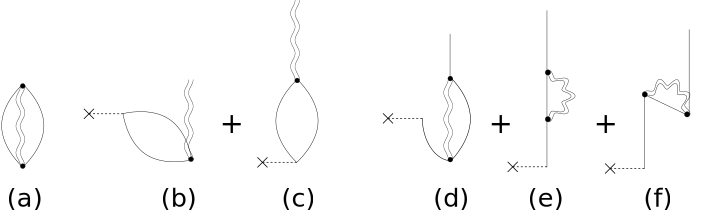
\includegraphics[width=\textwidth]{introduccion/figs/fig1_4_2.pdf}
\caption{Schematic representation of the NFT(s+r) diagrams at the basis of the characterization of a superfluid nucleus like e.g. $^{120}$Sn. \textbf{(a)} Nuclear structure (NFT(s)). Zero point fluctuations (ZPF) characterizing the nucleus ground state. Continuous lines describe quasiparticle (\textit{qp}) states, double wavy curves correlated two quasiparticle ($2qp$) vibrational modes. Because $\alpha^{\dagger}_{\nu}=U_\nu a^\dagger_\nu-V_\nu a_{\bar{\nu}}$ these modes encompass both particle--hole ($ph$) like vibrations, e.g. surface quadrupole vibrations, as well as correlated ($pp$) and ($hh$) monopole and multipole pairing vibrations. Intervening with an external field (cross followed by dashed line) one can excite (b) and (c) multipole ($ph$--like; inelastic scattering) and  pairing ($2p$--like) vibrations (two--particle transfer) as well as (d)-(f) single--quasiparticle states.}\label{fig1.4.2}
\end{center}
\end{figure}

 \begin{table}
\begin{center}
\begin{tabular}{|c|c|c|c|}
\hline
  Observables  &  SLy4 &  $d_{5/2}$ shifted  & Opt. levels \\ 
\hline
$\Delta$ &  10  (0.7\%) &  10  (0.7 \%) & 50   (3.5 \%)\\
 $E_{qp}$ & 190 (19\%)  & 160  (16\%)   & 45  (4.5 \%) \\
 Mult.  splitt. & 50  (7\%) & 70  (10\%)    & 59  (8.4 \%) \\
  $d_{5/2}$ strength (centr.) & 200  (20\%)  & 40  (4\%)   & 40  (4\%) \\
$d_{5/2}$ strength (width) & 160  (20\%)  &75  (9.3\%)  &  8  (1\%) \\
$B(E2)$ & 1.4  (14\%) & 1.34  (13\%)   & 1.43  (14\%) \\ 
$\sigma_{2n}(p,t)$ & 40 (2\%) & 40 (2\%) & 40 (2\%) \\
 %2n-transfer & 10 &10  & 10 \\ 
 \hline
\end{tabular}
\caption{Root  mean square deviation $\sigma$ between  the experimental data and the theoretical values expressed in keV for the pairing gap, quasiparticle energies, multiplet splitting, centroid and width of the  
$5/2^+$ low--lying single--particle strength distribution (Fig. \ref{fig6.2.3}). In single--particle units $B_{sp}$ for the $\gamma$-decay  (B(E2) transition probabilities) and in mb for $\sigma_{2n}(p,t)$ (Fig. \ref{fig8_2_4}). In brackets
the ratio $\sigma_{rel}=\sigma/L$ between $\sigma$ and the experimental  range $L$ of the corresponding quantities: 1.4 MeV ($\Delta$), 1 MeV ($E_{qp}$), 700 keV (mult. splitting), 
1 MeV ($d_{5/2}$ centroid),  809 keV (=1730--921) keV  ($d_{5/2}$ width), 10 $B_{sp}$ (B(E2)), 2250 $\mu$b ($\sigma_{2n}(p,t)$)) is given (for details see \cite{Idini:15}, also Fig. \ref{fig1.4.1}). Columns 2,3, and 4 contain the results of NFT calculations making use of bare single--particle levels from Hartree--Fock with Sly4, same but for a 600keV shift towards the Fermi energy of the $\epsilon_{d_{5/2}}$ orbital, and optimal values of $\epsilon_j$ for all valence levels so that the dressed quasiparticle states provide the best fit to that data, respectively.}
\label{tab1.4.1}
\end{center}
\end{table}


\section{Non--orthogonality}\label{appintroC}
Let us now consider a system based on a  closed shell nucleus, namely two protons moving around $^{208}$Pb.
The ground state of $^{210}_{84}\text{Po}_{126}$ can be viewed as the proton pair addition mode of the doubly closed shell nucleus  $^{208}_{82}\text{Pb}_{126}$, mode displaying $J^\pi=0^+$ and $\beta=+2$ (transfer--) quantum numbers. Within this framework $^{209}_{83}\text{Bi}_{126}$ is expected to be a \emph{bona fide} proton single--particle system ($\beta=+1$), in which the $g_{7/2},d_{5/2},h_{11/2},d_{3/2}$ and $s_{1/2}$ valence orbitals are occupied, the odd proton occupying, in the ground state, a substate of the $h_{9/2}$ orbital.



This picture can be specifically probed through one--proton stripping and pick up reactions, e.g. with the help of $^{210}$Po$(t,\alpha)^{209}$Bi and $^{208}$Pb$(^3$He$,d)^{209}$Bi transfer processes\footnote{It is of notice that in the present case, as well as in Sect. \ref{appintroA}, and at variance with the rest of the monograph, use will be made, for the sake of being didactic, of spectroscopic factors ( see end of Sect. \ref{C1S1} as well as App. \ref{C6AppI}).}. The pick--up reaction cross section is, in the case of e.g. the states $1/2^+(s_{1/2})$ and $11/2^-(h_{11/2})$,  essentially consistent with a single peak displaying full $(2j+1)$ occupancy. On the other hand, two $3/2^+$ states with essentially equal strength and exhausting the associated $(2j+1(=4))$ strength are observed.   Furthermore,  the four peaks mentioned above are essentially not excited in the stripping process (see Table \ref{tabintroC1}). In an attempt to further clarify the structure of the two $3/2^+$, use is made of the inelastic process $^{209}$Bi$(d,d')$. Both states are excited in  inelastic scattering, the associated  angular distributions  revealing the octupole character of such excitation (Tables \ref{tabintroC2} and \ref{tabintroC3}).

\begin{figure}
\centerline {
\includegraphics*[width=12cm]{introduccion/figs/figintroC1}
}
\caption{NFT diagram describing one of the most important processes coupling the $2p-1h$ states $\ket{\alpha}$ and $\ket{\beta}$ (see Eqs. (\ref{eqintroC1}) and (\ref{eqintroC2})), product of bare elementary modes of excitation consisting in the $^{208}$Pb, $0^+$ pair addition mode and the $d_{3/2}$ proton hole state, and of the lowest octupole vibration of $^{208}$Pb and of a proton moving in the $h_{9/2}$ orbital.}
\label{figintroC1}
\end{figure}
\begin{figure}
\centerline {
\includegraphics*[width=6cm]{introduccion/figs/figintroC2}}
\caption{Schematic representation of the $3/2^+$ states entering the NFT calculation of the process displayed in Fig. \ref{figintroC1}. The basis state $\ket \alpha$ carries the full $(t,\alpha)$ transfer strength ($tr$) $\sigma^{tr}$, while the basis state $\ket{\beta}$ the full octupole $(oct)$ strength $\sigma^{oct}$ (see Tables \ref{tabintroC1}--\ref{tabintroC3}). The overlap between these states is  $\cos \chi$. The physical states obtained through the (Feynman) diagramatic ``orthogonalization process'' are denoted $\ket{\text{I}}$ and $\ket{\text{II}}$ (see Eqs. (\ref{eqintroC3}) and (\ref{eqintroC4})).}
\label{figintroC2}
\end{figure}
In keeping with the fact that the same experiment reveals a multiplet (septuplet) of states with centroid around 2.6 MeV and with summed $L=3$ inelastic cross section consistent with that of the lowest collective  (2.615 MeV, $B(E3)/B_{sp}\approx 32$) octupole vibration of $^{208}$Pb, one can posit that the two $3/2^+$ states are a linear combination of the unperturbed (two particles)--(one hole) ($2p$--$1h$) states,
\begin{align}\label{eqintroC1}
\ket \alpha=\ket{d_{3/2}^{-1}\otimes gs (^{210}\text{Pb});3/2^+},
\end{align}
and 
\begin{align}\label{eqintroC2}
\ket \beta=\ket{h_{9/2}\otimes 3^- (^{208}\text{Pb});3/2^+}.
\end{align}
Because these states lie very close in energy they mix. According to NFT, the most important contribution to this mixing arises from the process given in Fig. \ref{figintroC1}. The resulting physical (mixed) states can be  written as,
\begin{align}\label{eqintroC3}
\ket {\text{I}}=-0.53 \ket \alpha + 0.76 \ket \beta,
\end{align}
and 
\begin{align}\label{eqintroC4}
\ket {\text{II}}=1.02 \ket \alpha + 0.80 \ket \beta,
\end{align}
as resulting from the calculation of the diagram displayed in Fig. \ref{figintroC1} to all orders of perturbation, with the help of Brillouin--Wigner perturbation theory (diagonalization of the corresponding effective Hamiltonian\footnote{See p. 316 \cite{Bortignon:77} and references therein.}, see Sect. \ref{Sect1.7.4}). 



Let us now calculate the overlap $\mathcal O=\braket{\alpha|\beta}$ between the basis states $\ket\alpha$ and $\ket{\beta}$, that is $\mathcal O=\cos\chi$ (see Fig. \ref{figintroC2}).   
\begin{table}
\begin{tabular}{|c|c|c|c|}
\hline 
 & $E_x$(MeV) & $S(t,\alpha)(2j+1)$ & $S(^3\text{He},d)$ \\
 \hline 
$3/2^+$ & 2.49 & $1.8\pm0.3\,(4)$  & $<0.01$  \\ 
$3/2^+$ & 2.95 & $2.2\pm0.3\,(4)$  & $<0.01$ \\ 
 $1/2^+$& 2.43 &  $1.8\,(2)$& $<0.02$ \\ 
 $11/2^-$& 3.69 & $10\,(12)$ &  $<0.05$\\ 
 \hline
\end{tabular}\caption{Single--particle strength associated with the  transfer reactions  $^{210}$Po$(t,\alpha)^{209}$Bi and $^{208}$Pb$(^3\text{He},d)^{209}$Bi (see \cite{Bortignon:77}).}\label{tabintroC1}
\end{table}
\begin{table}
\begin{tabular}{|c|c|c|}
\hline 
 & $E_x$(MeV) & $\frac{\sigma\left(^{209}\text{Bi}(9/2^-;gs)\rightarrow^{209}\text{Bi}(3/2^+;E)\right)}{\sigma\left(^{208}\text{Pb}(gs)\rightarrow (3^-;2.615\, \text{MeV})\right)}$  \\
 \hline 
$3/2$ & 2.49 & $0.042\pm0.003$   \\ 
$3/2$ & 2.95 & $0.011\pm0.002$  \\ 
 \hline
\end{tabular}\caption{The total inelastic cross section $\sigma^{oct}$ associated with the lowest octupole vibrational state of $^{208}$Pb can be written in terms of that associated with a single magnetic substate $\sigma'$ as $\sigma_{3^-}^{oct}=7\sigma'$. That associated with the multiplet $(h_{9/2}\otimes 3^-)_{J^+} (J=3/2-15/2)$ as $\sigma_{3^-}^{oct}=70\sigma'$, in keeping with the fact that the $h_{9/2}$ state has 10 magnetic substates. Thus, the strength associated with the 3/2 channel is 4/70=0.057 to be compared with the observed summed (percentage) strength $0.053\pm0.005 $ $(=(0.042\pm0.003)+(0.011\pm0.002))$ associated with the 2.45 MeV and the 2.95 MeV $3/2^+$ states; see \cite{Bortignon:77} Table 4.11.}\label{tabintroC2}
\end{table}
\begin{table}
\begin{tabular}{|c|c|c|c|c|c|c|c|c|}
\hline
& \multicolumn{2}{|c}{$E_n$(MeV)} & \multicolumn{2}{|c}{$\frac{\sigma(h_{9/2}\rightarrow 3/2^+)}{\sigma(0^+\rightarrow 3^-)}$(\%)} & \multicolumn{2}{|c}{$S(t,\alpha)$}  & \multicolumn{2}{|c|}{$S(^3\text{He},d)$}   \\
\hline
&Theory  & Exp  & Theory  & Exp & Theory & Exp & Theory  & Exp  \\
\hline
3/2& 2.480 & 2.494  & 3.76  & $4.2\pm0.3$  & 1.83  & $1.8\pm0.3$ &0.02  & $<0.01$  \\
3/2& 3.125 & 2.95  & 1.56 & $1.1\pm0.2$  & 2.25  & $2.2\pm0.3$ & $10^{-5}$  & $<0.01$  \\
\hline
\end{tabular}\caption{Summary of NFT predictions concerning the structure of the two lowest $3/2^+$ state of $^{209}$Bi, in comparison with the experimental data (see Table 4.7 of \cite{Bortignon:77}).}\label{tabintroC3}
\end{table}
Following this figure  one can write,
\begin{align}
\sqrt{\sigma_I^{tr}}=\cos\phi;\quad \sqrt{\sigma_{II}^{tr}}=\cos\left(\frac{\pi}{2}-\phi\right)=\sin \phi,
\end{align}
where
\begin{align}
{\sigma^{tr}}={\sigma_I^{tr}}+{\sigma_{II}^{tr}}=1,
\end{align}
in keeping with the fact that the absolute cross sections of the states $\ket {\text{I}}$ and $\ket {\text{II}}$ are normalized in terms of the total cross section.


In the same way
\begin{align}
\sqrt{\sigma^{oct}_I}=\cos(\chi-\phi)=\cos\chi\cos\phi+\sin\chi\sin\phi,
\end{align}
and
\begin{align}
\sqrt{\sigma^{oct}_{II}}=\cos\left(\pi-\left(\frac{\pi}{2}-\phi+\chi\right)\right)=-\cos\left(\frac{\pi}{2}+(\phi-\chi)\right)=\sin\phi\cos\chi+\sin\chi\cos\phi.
\end{align}
Thus
\begin{align}
\sqrt{\sigma^{oct}_{I}}=\cos\chi\sqrt{\sigma^{tr}_{I}}+\sin\chi\sqrt{\sigma^{tr}_{II}},
\end{align}
and
\begin{align}
\sqrt{\sigma^{oct}_{II}}=-\cos\chi\sqrt{\sigma^{tr}_{II}}+\sin\chi\sqrt{\sigma^{tr}_{I}}.
\end{align}
Multiplying the above relations by $\sqrt{\sigma^{tr}_{I}}$ and $\sqrt{\sigma^{tr}_{II}}$ respectively one obtains,
\begin{align}
\sqrt{\sigma^{tr}_{I}\sigma^{oct}_{I}}=\cos\chi\sigma^{tr}_I+\sin\chi\sqrt{\sigma^{tr}_{I}\sigma^{tr}_{II}},
\end{align}
and
\begin{align}
\sqrt{\sigma^{tr}_{II}\sigma^{oct}_{II}}=-\cos\chi\sigma^{tr}_{II}+\sin\chi\sqrt{\sigma^{tr}_{I}\sigma^{tr}_{II}},
\end{align}
which, upon substraction  leads to the  expression of the overlap
\begin{align}
\cos\chi=\frac{\sqrt{\sigma^{tr}_{I}\sigma^{oct}_{I}}-\sqrt{\sigma^{tr}_{II}\sigma^{oct}_{II}}}{\sigma_I^{tr}+\sigma_{II}^{tr}}.
\end{align}
Making use of the values of Tables \ref{tabintroC1}--\ref{tabintroC3} (see also Fig. \ref{figC1A7} (e) last column labeled \textit{experiment})\footnote{See Table 4.7 of \cite{Bortignon:77}.} one obtains
\begin{align}
\mathcal O=\cos\chi=\frac{\sqrt{1.8\times4.2}-\sqrt{2.2\times1.1}}{4}=0.298
\end{align}
  Regarding the NFT results related to  the above questions we refer to Sect. \ref{Sect1.7.4} as well as to App. \ref{App1.C} (Sect. \ref{AppCS2}). In what follows we provide  simple, necessarily qualitative estimates  making use of the relations\footnote{see Tables 4.5 and 4.6  \cite{Bortignon:77}.}.
\begin{align}
\nonumber &\braket{\text{I}|\text{I}}= (-0.53)^2+(0.76)^2-2\times0.53\times0.75\, \mathcal O=1,\\
\nonumber &\braket{\text{II}|\text{II}}= (1.02)^2+(0.80)^2+2\times1.02\times0.80\, \mathcal O=1,
\end{align}
and $\braket{\text{I}|\text{II}}=-0.53\times1.02+0.76\times0.80+(-0.53\times0.80+0.76\times1.02)\,\mathcal O=0$ leading to $\mathcal O=-0.18, -0.42$ and -0.19 respectively and, thus, to the average value of \mbox{$-0.26$}.
 Of course, one can hardly expect to obtain the sign to agree with that of the NFT expression, as it is associated with a free choice of the axis of references (Fig. \ref{figintroC2}). Note also the fact that the quantities $\sigma$ appearing above are well defined, while $\sqrt{\sigma}$ is indetermined by an overall sign.
\section{Coupling between intrinsic and relative motion}\label{appintroB}
In what follows, we consider the reaction
\begin{align}
a+A\rightarrow b+B,
\end{align}
within the framework of the semiclassical approximation\footnote{\cite{Broglia:04a} and references therein.}.
In the center--of--mass system, the total Hamiltonian may be written
\begin{align}\label{eqintroB2}
H=T_{aA}+H_a+H_A+V_{aA}=T_{bB}+H_b+H_B+V_{bA},
\end{align}
in keeping with energy conservation. Within this context other, mixed, representations are possible.

One then solves the time--dependent Schr\"odinger equation 
\begin{align}
i\hbar\frac{\partial \Psi}{\partial t}=H\Psi,
\end{align}
with the initial conditions that the nuclei $a$ and $A$ are in their ground states, and where the relative motion is described by a narrow wavepacket of rather well defined impact parameter and velocity.


We expand $\Psi$ on (stationary) channel wavefunctions 
\begin{align}
\Psi=\sum_{\beta}c_\beta\left(\left(\mathbf r_\beta-R_\beta\right)\right)\Psi_\beta e^{-iE_\beta t/\hbar},
\end{align}
where
\begin{align}
\Psi_\beta (t)=\Psi_m^b(\xi_b)\Psi_n^B(\xi_B)\exp(i\delta_\beta).
\end{align}
The index $\beta$ labels both the partition of nuclei $(b,B)$ as well as the quantal states of the two nucleons ($m,n$).


The phase $\delta_\beta$ is defined as
\begin{align}
\delta_\beta=\frac{1}{\hbar}\left\{m_\beta \mathbf v_\beta(t)\cdot \left(\mathbf r_\beta-\mathbf R_\beta(t)\right)-\int_0^t\left(U_\beta\left(R_\beta(t')\right)-\frac{1}{2}m_\beta\mathbf v_\beta(t')^2\right)\right\},
\end{align}
 where an extra phase has been added to eliminate, as far as possible, the diagonal matrix elements in the coupled equations.
The phase factor $\exp(i\delta_\beta)$ acting on the channel wavefunction is essentially a Galilean transformation (see jagged ``phonon'' in the NFT reaction diagrams displayed in Figs. \ref{fig6.1.1} (one--particle transfer) and Figs. \ref{figC7C1} and \ref{figC7C2} (two--particle transfer); see also Figs. \ref{figintro2}, \ref{figintro3} and \ref{fig1.9.2}--\ref{fig1.9.4}).



The function $c_\beta$ can be expressed as
\begin{align}
c_\beta=a_\beta(t)\chi_\beta(\mathbf r_\beta-\mathbf R_\beta(t),t)
\end{align}
product of an amplitude $a_\beta$ of asymptotic values ($t=\pm\infty$, 0 or 1), and a normalized shape (wavepacket) function, $R_\beta(t)$ being the relative motion elastic trajectory.


Properly combining the above quantities and making use of the time--dependent Schr\"odinger equation one obtains 
\begin{align}
i\hbar\sum_{\beta}\dot a_\beta(t)\langle\Psi_\xi|\Psi_\beta\rangle_{\mathbf R_{\xi\gamma}}e^{iE_\beta t/\hbar}=\sum_{\gamma}\langle\Psi_\xi|V_\gamma-U_\gamma(r_\gamma)|\Psi_\gamma\rangle_{\mathbf R_{\xi\gamma}}a_\gamma(t)e^{iE_\beta t/\hbar},
\end{align}
where
\begin{align}
f(\mathbf R)=\langle\Psi_\xi|V_\gamma-U_\gamma(r_\gamma)|\Psi_\gamma\rangle_{\mathbf R}
\end{align}
are the formfactors, and
\begin{align}
g(\mathbf R)=\langle\Psi_\xi|\Psi_\beta\rangle_{\mathbf R}
\end{align}
the \textit{overlaps between the intrinsic channel wavefunctions}.



The coupled equations can be written in a more compact form by introducing the adjoint channel wavefunction 
\begin{align}
\omega_\xi=\sum_{\gamma}g_{\xi\gamma}^{-1}\Psi{\gamma},
\end{align}
where $g^{-1}$ is the reciprocal of the \textit{overlap matrix}
\begin{align}
g_{\xi\gamma}=\langle\Psi_\xi|\Psi_\gamma\rangle.
\end{align}
Thus
\begin{align}
(\omega_\xi,\Psi_\beta)=\delta(\xi,\beta),
\end{align}
and
\begin{align}
i\hbar\dot a_\beta(t)=\sum_{\gamma}\langle\omega_\beta|V_\gamma-U_\gamma|\Psi_\gamma\rangle_{\mathbf R_{\beta\gamma}}e^{(E_\beta-E_\gamma)t/\hbar}a_\gamma(t).
\end{align}
Consequently, the proper tunneling Hamiltonian is obtained by a \textit{basis orthogonalization process}. These coupled equations, being first order in time, can be solved knowing the initial conditions at time $t=-\infty$,
\begin{align}
a_\gamma(-\infty)=\delta(\gamma,\alpha),
\end{align}
where $\alpha$ labels the entrance channel, that is, the nuclei $a$ and $A$ in their ground state. The cross section for the reaction $\alpha\rightarrow\beta$ is
\begin{align}
\left(\frac{d\sigma}{d\Omega}\right)_{\alpha\rightarrow\beta}\sim\left|a_\beta(t=+\infty)\right|^2.
\end{align}



\section{Nuclear Field Theory for pedestrians}\label{appintroA}

Nuclear Field Theory (NFT) was tailored after Feynman's graphical version of quantum electrodynamics (QED)\footnote{``The diagrams were intended to represent physical processes and the mathematical expressions to describe them\dots I would see electrons going along, being scattered at on point\dots emitting a photon and the photon goes over there\dots I thought that if they really turn out to be useful it would be fun to see them in the pages of Physical Rview'' R. P. Feynman.}. It is then natural that in discussing NFT analogies with QED will be recurrent.   Arguably, as a consequence of special relativity which put an end to the concept of ether, the field--free and matter--free vacuum was rightly considered as \textit{bona fide} empty space. The advent of quantum mechanics changed this situation, the vacuum becoming populated. In quantum mechanics an oscillator, for example, cannot be at rest. The oscillatory nature of the radiation field requires zero point fluctuations (ZPF) of the electromagnetic fields in the vacuum state of lower energy. The occupation of the negative kinetic energy electron states and the subsequent calculation of the cross section for pair creation by photons, contributed another step in the understanding of the QED vacuum, let alone the Lamb shift\footnote{In high energy collisions and accelerator laboratories some of the original beam energy can be consumed by ripping electron-positron pairs out of the vacuum (\cite{Bruce:07}).}.


When the fields are expressed in terms of creation and annihilation operators, the interaction between  fermion and boson fields is proportional to the product of two fermion creation or destruction operator $a^\dagger$ or $a$, and of one boson operator $\Gamma^\dagger$ or $\Gamma$: e.g. $a^\dagger_{\nu'}a_\nu\Gamma_\alpha^\dagger$, (see Fig. \ref{figintroA1}). That is,  bilinear in the fermion fields and linear in the boson fields.

\begin{figure}
\centerline {
\includegraphics*[width=12cm]{introduccion/figs/figintroA1}
}
\caption{Oyster diagrams describing the correlation of the nuclear ground state associated with the ZPF of  collective particle--hole--like excitations. In (a) we show two of such diagrams. In (b) and (c) we display a symmetrized (boson exchange), and antisymmetrized  (fermion exchange) correction to (a), while  (d) contains a simultaneous boson and fermion exchange. In all the diagrams shown, only ground state correlation vertices are present. They are connected with the $Y^\alpha_{k_i}$--components ($\epsilon_k>\epsilon_F, \,\epsilon_i\le\epsilon_F$) of the RPA wavefunction describing the collective mode (wavy line). While this is so for any time ordering, i.e., the sequence with which the particle-vibration coupling vertex (black dot) appear in the case of the processes shown in (a) and (b), this is not the case in connection with processes shown in (c) and (d) as can be seen from the corresponding diagrams (c') and (d') shown in the inset. Because of Pauli principle between particles (holes) present and those involved in the collective modes, the harmonic approximation has to be corrected. This is diagramatically reflected by the presence of scattering vertices.}
\label{figintroA1}
\end{figure}
\begin{figure}
\centerline {
\includegraphics*[width=10cm]{introduccion/figs/fig1_7_2}
}
\caption{Some of the possible outcomes resulting from acting with an external single--particle field, i.e. that associated with inelastic processes (represented by a horizontal dashed line starting with a $\times$) on the ZPF of a nucleus ground state associated with particle--hole correlated vibrations. Within this context one returns to the question of  renormalization mentioned in the text (see end of Sect. \ref{S1.1} and Sect. \ref{C1S4}, see also \cite{Idini:15}, \cite{Broglia:16}, \cite{Barranco:17}; see also Sect. \ref{C6S4}) The diagrams of the first row result by intervening the virtual process shown in Fig. \ref{figintroA1} (c) and eventual time orderings. Similar for those of the second row but in connection with diagram (b) of Fig. \ref{figintroA1}. The boxed processes correspond to particle self--energy (first row) and vertex correction (second row). Reversing the sense in which the fermions (arrowed lines) circle the loop from anticlockwise to clockwise, one obtains two new graphs. The complete set of processes obtained in this way are shown in the third and last row, and constitute a sum rule conserving set of diagrams.}
\label{figintroA2}
\end{figure}
\clearpage
\begin{figure}[h!]
\centerline {
\includegraphics*[width=10cm]{introduccion/figs/figintroA3}
}
\caption{ZPF associated with the pair addition mode taking into account the interweaving of nucleons with density modes. The processes boxed in (g), (k) and (o), are associated with the induced pairing interaction (medium polarization effects; (p), (q), (r)) resulting from the exchange of density modes between nucleons moving in time reversal states, including also vertex corrections. The two--nucleon stripping and pickup external field is labeled by a dashed horizontal line which starts with a $\times$. The possibility of using pairing vibrational modes as intermediate bosons contributing to the induced pairing interaction, not only in $^1S_0$ channels but also in other channels (multipole modes) is discussed in App. \ref{App6G}. In particular, in connection with the possible presence of ``vortex--like'' pair addition modes, in exotic, halo nuclei, with $J^\pi=1^-$ and $\beta=+2$ quantum numbers.}
\label{figintroA3}
\end{figure}
\clearpage

A detailed graphical NFT treatment of the vacuum has an important consequence concerning the probing of nuclear structure with reactions. By intervening it with an external field one will excite the modes whose properties can be  compared with experiment without further ado. 

In other words, if one is in doubt of which are the properly dressed elementary, physical modes of excitation, one should find out how to specifically excite the  mode in question, by acting with an external field on the ZPF of the vacuum (Hawking--like radiation\footnote{\cite{Barranco:19b}.}; see also Sect. \ref{S6.6.2} in particular Fig. \ref{fig6.6.2}). That is,  carry out a \textit{gedanken}, NFT--like \textit{experiment} as in Fig. \ref{figintroA2} for $p-h$--vibrations and in Fig. \ref{figintroA3} regarding pairing vibrations. Because the corresponding processes deal  with physical states, they translate with ease into a laboratory setup. In keeping with the fact that the vacuum contains all the information (right physical degrees of freedom) of the quantal system under study. Forcing virtual processes associated  with vacuum ZPF to become real, one is guaranteed to get, in each instance, the real, dressed, physical particle. 

The fact that one can treat fully quantum mechanically and on equal footing both structure and reaction processes is apparent from these figures and considerations\footnote{Full fledge embodiments being found in e.g. Figs. \ref{fig1.9.1} and \ref{fig1.9.2} and Figs. \ref{fig6.3.1} and \ref{fig6.6.2}.}. Thus unification of structure and reactions, and dressing of energies, vertices (interactions) and formfactors (single--particle radial wavefunctions and associated transition densities), results in a single vacuum correlated state (e.g. Figs. \ref{figintroA1} and \ref{figintroF2}). Vacuum states which through its fluctuations, reflect both single--particle, normal and abnormal (pairing) density vibrations and their interweaving.  It also indicates the  set of specific probes which make  these virtual states to collapse into on--the--energy shell states, providing the corresponding physical information to the   outgoing particles, also photons, which eventually interact with the corresponding detectors (e.g. Figs. \ref{figintroA2}, \ref{figintroA3} and \ref{fig1.9.2}). Structure and reaction processes free of non--orthogonality, overcompleteness and Pauli violation contributions.


Summing up, the last line of Fig. \ref{figintroA2} displays, together with the corresponding time orderings, the lowest order self--energy and vertex correction renormalising vibrational states. It thus gives rise to the physical collective vibrations whose properties can be directly compared with the experimental findings (within this context see last paragraph of the next section). In other words, the processes shown in the last line of   Fig. \ref{figintroA2} imply that the elementary modes participating in the virtual states have to display, exception made for energy (off--shell modes) the same properties of the physical, dressed (renormalized), on--shell modes whose properties can be directly compared with experiment\footnote{Examples of these processes in the case of giant resonances are found in \cite{Bortignon:81,Bertsch:83}. For low--lying states see \cite{Barranco:04}.} (renormalized NFT). This because one can, through an experiment
force such virtual states to become real (on--shell) on short call.

Let us now provide an introduction to NFT for pedestrians and see how the above considerations become concretely implemented\footnote{For details we refer to \cite{Bortignon:77} and refs. therein.}
\subsection[The concept of elementary modes of excitation]{The concept of elementary modes of excitation\protect\footnote{\cite{Bes:77}}}\label{C1S7.1}
The Hamiltonian of a many--body system of noninteracting particles, bosons or fermions, can be written as
\begin{align}\label{eqC1A1}
H=\sum_iH_i,
\end{align}
where the summation is over all the particles of the system and where each $H_i$ depends only on the variables of the $i$--th particle. The single--particle Schr\"odinger equation is
\begin{align}\label{eqC1A2}
H_i\psi_k(\mathbf r_i)=\epsilon_k \psi_k(\mathbf r_i),
\end{align}
where $\epsilon_k$ is the single--particle energy eigenvalue and 
\begin{align}\label{eqC1A3}
\psi_k(\mathbf r_i)\equiv\bra{\mathbf r_i}a_k^\dagger\ket{0}
\end{align}
is the corresponding wave function. The operator $a_k^\dagger$ creates a particle in the state $k$ when acting in the vacuum state $\ket{0}$. The energy levels of the system are given by the equation
\begin{align}\label{eqC1A4}
E_n=\sum_k n_k\epsilon_k,
\end{align}
the corresponding eigenstates being
\begin{align}\label{eqC1A5}
\ket{n}=\prod_k\frac{(a_k^\dagger)^{n_k}}{\sqrt{n_k!}}\ket{0},
\end{align}
where $n_k=0$ or 1 in the case of fermions and $n_k=0,1,2,\dots$ in the case of bosons.

Now we consider a system of interacting particles. The Hamiltonian will in this case be
\begin{align}\label{eqC1A6}
H=\sum_i H_i+\frac{1}{2}\sum_{i,j}H_{ij},
\end{align}
where $i,j$ label the co--ordinates of the $i$--th and $j$--th particle.

In some cases it is possible to recast the two--body Hamiltonian in the form
\begin{align}\label{eqC1A7}
H=\sum_\tau H'_\tau,
\end{align}
with the associated Schr\"odinger equation
\begin{align}\label{eqC1A8}
H'_\tau\psi_\tau(\zeta)=\epsilon_\tau \psi_\tau(\zeta),
\end{align}
$\zeta$ representing a general variable\footnote{Collective, also in the sense of independent particle motion (see \cite{Mottelson:62}) variable or order parameter.} (e.g. the single--particle co--ordinate, the gap parameter, the shape of the nucleus, etc.). The wave function $\psi_\tau(\zeta)$ is the $\zeta$--co--ordinate representation of the eigenstate $\alpha_\tau^\dagger\ket{\tilde 0}$. The operator $\alpha_\tau^\dagger$ creates an excitation with the quantum number $\tau$ when acting in the state $\ket{\tilde 0}$, the correlated vacuum of all the excitations $\tau$.



The energy of the levels of the system, or at any rate of the most important
ones to determine the physical response of it to external probes can be written
in the form
\begin{align}\label{eqC1A9}
E_m=\sum_{\tau}n_\tau \epsilon_\tau.
\end{align}
The corresponding eigenstate can be written in the same way as before, \textit{i.e.}
\begin{align}\label{eqC1A10}
\ket{n}=\prod_\tau\frac{(\alpha_\tau^\dagger)^{n_\tau}}{\sqrt{n_\tau!}}\ket{\tilde 0}.
\end{align}
Additivity features similar to (\ref{eqC1A9}) hold for other physical quantities, \textit{i.e.}
\begin{align}\label{eqC1A11}
\braket{n|\mathcal O|m}=\sum_{\tau}A_\tau\sqrt{n_\tau} \delta(n_\tau,m_\tau+1),
\end{align}
where
\begin{align}\label{eqC1A12} O=\sum_{\tau}A_\tau \alpha_\tau^\dagger
\end{align}
is the operator which specifically excites the eigenstates described by $\psi_\tau(\xi)$.
Because the excitation energies $E_m$ and observables $\left|\braket{m'|\mathcal O|m}\right|^2$ (e.g. absolute two--particle transfer cross--section, electromagnetic-transition probabilities, etc.) are
linear combinations of $\epsilon_\tau$ and $A_\tau$, respectively, the eigenstates with energy $\epsilon_\tau$
and associated observable $A_\tau$ are called the \textit{elementary excitations of the system}.


The elementary modes of excitation  of a many-body system  represent a generalization of  the idea of normal modes of vibration.
They provide the building blocks of the excitation spectra, giving  insight  into the  deep nature  of the system one is studying, aside from allowing 
for an economic description  of complicated spectra in terms of a gas of, as a rule, weakly interacting bosons and fermions. In the nuclear case 
they correspond to clothed particles and empirically renormalised vibrations (rotations).

There lie two ideas behind the concept of elementary modes of excitation\footnote{This concept was introduced by Landau (\cite{Landau:41}) to describe the spectrum of HeII. It was subsequently utilized by Bohr and Mottelson (\cite{Bohr:75}) to obtain a unified description of the nuclear spectrum.}. First, that one does not need to be able to calculate the total binding
energy  of a nucleus to accurately describe the low energy excitation spectrum, in much the same way in which one can calculate 
the normal modes of a metal rod not knowing how to  calculate its total cohesive energy.
The second idea is that low-lying states ($\hbar \omega \ll \epsilon_F \ll BE$, i.e. binding energy) are of a particularly simple
character, and are amenable to a simple treatment, their
interweaving  being carried out at profit, in many cases,  in perturbation theory
\footnote{More precisely, and in keeping with  the fact that 
boson degrees of freedom have to decay through linear particle--vibration 
coupling vertices of strength $\Lambda$ into their fermionic components to interact with another vibrational mode,
the interweaving between the variety of many-body components clothing a single-particle state 
or a collective vibration will be described at profit in terms of an arrowed matrix which, assuming perturbation theory
to be valid, can be transformed, neglecting contributions of the order of $\Lambda^3$ or higher, into a co-diagonal matrix, namely a matrix 
whose non-zero elements are $(i,i-1)$ and $(i,i+1)$,  aside from  the diagonal ones $(i,i)$.}. 
Within this context it is  necessary to have a microscopic description 
of the ground  state of the system  which ensures that it acts as the vacuum state 
$|\tilde0\rangle  $ of the elementary modes of excitation. In other words $a_{\nu}|\tilde 0 \rangle   = 0, \Gamma_{\alpha} |\tilde 0\rangle   =0$, where
$a^+_{\nu}|\tilde 0 \rangle   = |\nu\rangle  $ and , $\Gamma^+_{\alpha} |\tilde 0\rangle   =|\alpha\rangle  $ represent a single-particle and a one-phonon state.
This   implies, in keeping 
with the indeterminacy  relations\footnote{The quantities $I$, $N$ and $\Omega$, $\phi$ are the angular momentum and particle number, conjugate variables to the Euler and gauge angles respectively.} $\Delta x \Delta p \geq \hbar/2$, $\Delta I \Delta \Omega \geq 1$, $\Delta N \Delta \phi \geq 1$, etc.  that $|\tilde 0\rangle   = |0\rangle  _F |0\rangle  _B$
displays the  quantal zero point fluctuations (ZPF) of the many--body system under study.

Within the framework of nuclear field theory (NFT) used below, in which single-particle (fermionic, F) and vibrational
(bosonic, B) elementary modes of excitation are to be calculated within the framework of HFB and QRPA
respectively, $|\tilde 0\rangle  $ must display the associated ZPF (cf. App. \ref{App1.E}). In particular for (harmonic) vibrational modes the indeterminacy relation achieves its lowest possible value 
$\Delta x \Delta p = \hbar/2$, the associated zero point energy amounting to $\hbar \omega/2$
for each degree of freedom. For example 5$\hbar \omega/2$ for quadrupole vibrations, 
$\hbar \omega$ being the energy of the collective vibrational mode under consideration. 




An illustrative example of the above arguments is provided by the low--lying quadrupole vibrational state of $^{120}$Sn. 
Diagonalizing SLy4 in QRPA leads to a value of $B(E2)$
(890 $e^2$ fm$^2$) which is about a factor of 2 smaller than experimentally observed (2030 $e^2$ fm$^2$). 
Taking into account  renormalisation effects in NFT, 
namely in a conserving  approximation (self-energy and vertex corrections, generalised Ward identities, see last line of Fig. \ref{figintroA2} and  Fig. \ref{fig6_C3x}), one obtains a value (2150 e$^2$ fm $^2$), 
which essentially coincides with 
the experimental findings. One does not know how to accurately calculate the absolute ground state energy 
$E_0$ (total binding energy) of e.g. $^{120}$Sn, but one can accurately work out 
the properties of the low--energy mode of this nucleus, also the collective energies 
$\hbar \omega_L =E_L - E_0$, and thus the associated ZPF and zero point energy $E_0$,
by renormalizing  QRPA solutions through self--energy and vertex corrections contributions\footnote{\cite{Barranco:04}, \cite{Bortignon:81}.}. 
Now, if the collective phonons are not the main object  of the study, but are to be used to cloth the single-particle states 
and give rise to the induced pairing interaction, one can make 
use of phonons which account for the experimental findings (renormalization\footnote{\cite{Idini:15,Broglia:16,Barranco:17}.})\footnote{As already mentioned, with the help of experimental probes which couple weakly to the nucleus,
i.e. in such a way that the system can be expressed in terms of the properties
of the excitation in the absence of probes (see however Sect. \ref{S6.5.4}), it has been possible to identify the
following elementary excitations in systems around closed shells:
\begin{enumerate}[a)]
\item single--particle and --holes,
\item shape vibrations,
\item spin and isospin vibrations and charge exchange modes,
\item pairing vibrations.
\end{enumerate}
Away from closed shells one has to add to the above modes:
\begin{enumerate}[a)]
\setcounter{enumi}{4}
\item rotations in 3D--space (e.g. quadrupole rotations)
\item rotations in gauge space (pairing rotations).
\end{enumerate}
Different probes have been utilized in the process of the identification of the different modes. In particular two-neutron transfer reactions induced by tritons
and protons have played a central role in unraveling the basic features of the pairing modes.}.




 
\subsection{NFT rules and applications}\label{Sect1.7.2}
A field theory can be formulated in which the nuclear elementary modes of
excitation play the role of the free fields and in which their mutual interweaving takes place through the particle--vibration coupling vertices\footnote{\cite{Bes:74,Broglia:76,Bohr:75,Mottelson:76}.}.
This theory provides a graphical perturbative approach to obtain the exact
solution of the many-body nuclear-structure problem in the product basis $\psi_\tau(\zeta)\psi_\eta(\Delta)\dots\psi_\gamma(\Gamma)$


Note that the nuclear bosonic fields are built out by utilizing those degrees
of freedom (particles and holes) which already exhaust all the nuclear degrees
of freedom. It is thus an essential feature of the product basis to be over-
complete and to violate the Pauli principle. On the other hand, this basis is
directly related to observables of the system. The different experiments project out only one or two of its components.


In what follows we state and apply the nuclear--field--theory rules, to calculate the interactions between the nuclear free fields and the reaction processes
between the resulting physical states making use of a schematic model. \subsubsection{Schematic model}
The model considered consists of two single--particle levels, each with pair degeneracy\footnote{It is of notice the difference of a factor of 2 in the degeneracy of each level as compared to Sect. 2 of \cite{Bortignon:77} in which case it is $2\Omega$. This is in keeping with the fact that, as a rule, $\Omega=(2j+1)/2$. See also Eq. (\ref{eqC1A86}) and related discussion. \label{fnlabel}} $\Omega$ and with a schematic monopole particle--hole interaction coupling the particles in the two levels.

The total Hamiltonian is equal to
\begin{align}\label{eqC1A13} 
H=H_{sp}+H_{TB}
\end{align}
where
\begin{align}\label{eqC1A14} 
H_{sp}=\frac{\epsilon}{2}N_0,\quad\quad N_0=\sum_{\sigma=\pm 1,m}\sigma a^{\dagger}_{m,\sigma}a_{m,\sigma},
\end{align}
and
\begin{align}\label{eqC1A15} 
H_{TB}=-\frac{V}{2}\left(A^\dagger A+AA^\dagger\right),\quad\quad A^\dagger=\sum_m a^\dagger_{m,1}a_{m,-1}.
\end{align}


The index $\sigma$ (=$\pm1$) labels the two levels, while $m$ labels the degenerate states within
each level. The strength of the monopole coupling is denoted by $V$ and the
energy difference between the two levels is $\epsilon$. 
The matrix element of (\ref{eqC1A15}) is given by
\begin{align}\label{eqC1A16} 
\braket{m,1;m',-1|H_{TB}|m'',1;m''',-1}=-V\delta(m,m')\delta(m'',m''').
\end{align}
\subsubsection{Field--theoretical solutions}
 The bare nuclear  fields are
the elementary modes of excitation comprising surface vibrations and single
particles. The boson fields are defined through the random--phase
approximation, in terms of particle-hole excitations. The basis utilized to
describe the nuclear systems is a product of the different free fields. 
The closed-shell system of the schematic model under consideration corresponds to the lowest ($\sigma = - 1$) level filled with $\Omega$ particles, while the upper
($\sigma =  1$) level remains empty. The basis particle and hole states are obtained
by adding or removing a single particle to/from this closed-shell configuration.
The corresponding wave functions and energies, which should include the
Hartree-Fock corrections (see Fig. \ref{figintro4} (b), (c)) generated by the residual interaction\footnote{The Hartree--Fock energy associated with the Hamiltonian (\ref{eqC1A13}) can be obtained
from the linearization relation $[H,a_{\sigma,m}^\dagger]=E(m,\sigma)a^\dagger_{\sigma,m}$ acting on the Hartree--Fock
vacuum, which in this case coincides with the single-particle vacuum defined by
 $a^\dagger_{m,-1}\ket{0}=a_{m,1}\ket{0}=0$}, are
 \begin{align}\label{eqC1A17} 
\left\{\begin{array}{l}
 \ket{m,1}=a^\dagger_{m,1}\ket{0},\quad E(m,1)=\frac{1}{2}(\epsilon+V),\\ 
\ket{m,-1}=a^\dagger_{m,-1}\ket{0},\quad E(m,-1)=\frac{1}{2}(\epsilon+V).
\end{array} \right.
 \end{align}
Thus the unperturbed energy for producing a particle-hole excitation with
respect to the ground state is
 \begin{align}\label{eqC1A18} 
\epsilon'=E(m,1)+E(m,-1)=\epsilon+V.
 \end{align}
 \begin{figure}
 \centerline {
 \includegraphics*[width=4cm]{introduccion/figs/fig18}
 }
 \caption{Graphical representation of the amplitude of the collective phonon (wavy line) on a given particle--hole excitation ($(m,1),(m,-1)$). This amplitude can be written in terms of the interaction vertex denoted by $\Lambda_i$, and the energy denominator $\omega_i-\epsilon'$. The particles (holes) are depicted by upward-- (downward--) going arrowed lines.}
 \label{figC1A1}
 \end{figure}
The contribution $V$ in (\ref{eqC1A18}) is the Hartree--Fock contribution to the particle--hole excitation.

If we define the creation operator of the normal modes as
 \begin{align}\label{eqC1A19} 
\beta^\dagger_\nu=\sum_m \lambda_m^\nu a_{m,1}^\dagger a_{m,-1},
 \end{align}
the linearization equation
 \begin{align}\label{eqC1A20} 
[H,\beta_\nu^\dagger]=\omega_\nu\beta^\dagger_\nu,
 \end{align}
yields
 \begin{align}\label{eqC1A21} 
\left\{\begin{array}{l}
 \omega_1=\epsilon'-V\Omega,\\ 
\omega_\nu=\epsilon'\quad (\nu=2,3,\dots,\Omega).
\end{array} \right.
 \end{align}
Utilizing (\ref{eqC1A20}) and the normalization condition
 \begin{align}\label{eqC1A22} 
[\beta_\nu,\beta^\dagger_{\nu'}]=\delta(\nu,\nu'),
 \end{align}
we obtain for the amplitudes associated with the lowest mode
 \begin{align}\label{eqC1A23} 
\lambda_m^1=\frac{1}{\sqrt{\Omega}}.
 \end{align}
One can also write this amplitude as the ratio between a coupling matrix
element and an energy denominator, i.e.
 \begin{align}\label{eqC1A24} 
\lambda_m^1=\frac{\Lambda_1}{\omega_1-\epsilon'}.
 \end{align}
From (\ref{eqC1A21}), (\ref{eqC1A23}) and (\ref{eqC1A24}) we obtain
 \begin{align}\label{eqC1A25} 
\Lambda_1=-V\sqrt{\Omega},
 \end{align}
which is the strength with which a particle~hole excitation $(m, 1; m, -1)$
couples to the collective phonon (see Fig. \ref{figC1A1}). This can also be seen by calculating
the matrix element of the interaction Hamiltonian (\ref{eqC1A15}) between the normal
modes and the single particle-hole state
 \begin{align}\label{eqC1A26} 
\Lambda_\nu=\braket{n_\nu=1|H_{TB}|m,1;m',-1}=-V\sqrt{\Omega}\,\delta(m,m')\,\delta(\nu,1).
 \end{align}
Note that the particle--vibration coupling strengths associated with the other
normal modes lying at an energy $\epsilon'$ (see (\ref{eqC1A21})) are equal to zero. The exact solution of (\ref{eqC1A13}) is reproduced by utilizing
as the basic degrees of freedom both the vibrations (see (\ref{eqC1A21})) and the particles
(see (\ref{eqC1A17})) coupled through the interactions (\ref{eqC1A16}) (four--point vertex) and (\ref{eqC1A26}) (particle--vibration coupling)\footnote{\cite{Bes:74,Broglia:76}}. A significant
part of the original interaction has already been included in generating the
collective mode (\ref{eqC1A21}). This implies that the rules for evaluating the effect of
the couplings (\ref{eqC1A16}) and (\ref{eqC1A26}) between fermions and bosons involve a number of restrictions as compared with the usual rules of perturbation theory that
are to be utilized in evaluating the effect of the original interaction (\ref{eqC1A15}) acting
in a fermion space. They read as follows:
\begin{enumerate}[I)]
\item In initial and final states, proper diagrams involve collective modes
and particle modes, but not any particle configuration that can be replaced by
a combination of collective modes. This restriction permits an initial state
comprising the configuration ($n_\nu =1;m$), but excludes ($m', 1; m',-1; m,1$).
\item The couplings (\ref{eqC1A16}) and (\ref{eqC1A26}) are allowed to act in all orders to
generate the different diagrams of perturbation theory; the restriction I) does
not apply to internal lines of these diagrams.
\item The internal lines of diagrams are, however, restricted by the exclusion of diagrams in which a particle--hole pair is created and subsequently
annihilated without having participated in subsequent interactions.
\item The energies of the uncoupled particle and phonon fields are to be
calculated by utilizing the Hartree--Fock approximation (see eq. (\ref{eqC1A17})) and the
RPA (see eq. (\ref{eqC1A21})), respectively. The contributions of all allowed diagrams are
evaluated by the usual rules of perturbation theory.
\end{enumerate}

We note that the external fields acting on the system are allowed to create
any state which may generate the different diagrams of perturbation theory.
The corresponding matrix elements should be weighted with the amplitude of
the component through which the final state is excited.



The above rules are also valid for those situations which cannot be treated
in perturbation theory and where a full diagonalization is called for. Thus,
\textit{e.g}., when the system displays a spurious state (see Sect. \ref{C1S7sS3}).



In what follows we discuss the energy of the $2p-1h$--like excitations, simplest modes which can display spuriousity. We
distinguish between two types of states, namely
 \begin{align}\label{eqC1A27} 
\ket{n_i=1;m,1},\quad\left\{
\begin{array}{ll}
\omega_1=\epsilon'-V\Omega, &\Lambda_1=-\sqrt{\Omega}V\\
&(i=1;m=1,2,\dots,\Omega),  \\ 
\omega_i=\epsilon', &\Lambda_i=0\\
&(i=2,\dots,\Omega; m=1,2,\dots,\Omega),
\end{array} \right. 
 \end{align}
and\footnote{Since the states (\ref{eqC1A28}) are restricted to be intermediate states of the perturbation
expansion, the configuration ($m,1;m,-1;m',1$) is allowed.}
 \begin{align}\label{eqC1A28} 
\ket{m',1;m',-1;m,1},\quad\epsilon'\quad(m,m'=1,2,\dots,\Omega),
 \end{align}
 where as in (\ref{eqC1A27}) only the energy of the particle--hole excitation is given (see (\ref{eqC1A18})). One can also displace the zero point of the odd system to the value $\epsilon/2$, in which case the unperturbed energy of the basis states $\ket{n_i;m,1}$ is $\omega_i$.
The physical states are to be written as
 \begin{align}\label{eqC1A29} 
\ket{qm}=\sum_i\xi_{iqm}\ket{n_i=1;m,1},
 \end{align}
  \begin{figure}
  \centerline {
  \includegraphics*[width=12cm]{introduccion/figs/fig19}
  }
  \caption{Contributions to the interaction of a fermion and a collective boson $\omega_i$ to order $1/\Omega^4$. The secular equation $E-E^{(0)}=A\sum_na^n(-1)^n$ is given in terms of the quantities $A=4\Omega V^2/(3\epsilon'-2E)$ and $a=2V/(3\epsilon'-2E)$. The hatched circle represents the (particle--hole) four--point vertex (\ref{eqC1A16}) (see Fig. \ref{figC1A4}, third and fourth diagrams).}
  \label{figC1A2}
  \end{figure}
as (\ref{eqC1A28}) cannot be basis states according to rule I), but only intermediate
states. The quantities $\xi_{iqm}$, are the amplitudes of the physical state in the different components of the product basis of elementary excitations. Rule (I) eliminates most of the double counting of two--particle, one--hole states. The model state contains $\Omega$ ``proper'' states of the form $\ket{n_i;m,1}$,  in which case the odd particle is in the state $(m,1)$. That is $\ket{n_1;m,1}$ ($\omega_1=\epsilon'-V\Omega$) and $\ket{n_i;m,1}$ ($\omega_i=\epsilon',\; i=2,\dots,\Omega$). However, there are only $\Omega-1$ two--particle, one--hole states in which the odd particle is in the state $(m,1)$ (Fig. \ref{figalpha}). Therefore, a spurious state remains in the spectrum based on elementary modes of excitation. In other words, allowing the quantum number $m$ to run over all possible $\Omega$--states, the  model space contains $\Omega^2$ states (one for each value of $m$), while the correct number is $\Omega(\Omega-1)$.


  \begin{figure}
  \centerline {
  \includegraphics*[width=13cm]{introduccion/figs/figalpha}
  }
  \caption{Schematic two--level model. Count of the states $\ket{m,1;m-1;m',1}$ in the case of $j=3/2$ and $\Omega=2j+1=4$. State (b) is not allowed because of Pauli principle. The states ((a),(e)), ((c),(f)) and ((d),(g)) are pairwise identical, in keeping with the indistinguishability of the particles. Thus, the states (a), (c) and (d) (equivalent (e), (f) (g)) exhaust the degrees of freedom of states of type (\ref{eqC1A28}). In other words, there are only $\Omega-1=3$ two--particle one--hole states in which the odd particle is in the state ($m',1$).}
  \label{figalpha}
  \end{figure}
Thus the basis $\ket{n_1=1; m,1}$ contains $\Omega$ spurious states. Its origin can be
traced back to the violation of the Pauli principle (see also Sect. \ref{C1S7sS3}).
To obtain the energy of $\ket{qm}$ we have to allow the states $\ket{n_1=1;m,1}$
to interact through the vertices (\ref{eqC1A16}) and (\ref{eqC1A26}) and generate all the different
perturbation theory diagrams (see rule II)) except those containing bubbles
(see rule III)).


The different graphical contributions calculated in the framework of the
Brillouin--Wigner perturbation theory are displayed in Fig. \ref{figalpha}. There is only
one (diagonal) matrix element given by a single summation, which can be
carried to all orders in the interaction vertices\footnote{Concerning the proper expansion parameter see Sect. \ref{Sect1.7.4}, Eq. (\ref{eqC1A86}).}, and can be written as
 \begin{align}\label{eqC1A31} 
\nonumber X_{ii'}=A\sum_n&(-1)^na^n\delta(i,i')=\\
&=\frac{A}{1+a}\delta(i,i')\delta(n,1)=-K(E)(\sqrt{\Omega}V)^2\delta(i,i')\delta(i,1),
 \end{align}
where a and A are defined in the caption to the figure and
 \begin{align}\label{eqC1A32} 
K(E)=\left(\tfrac{3}{2}\epsilon'-E+V\right)^{-1}.
 \end{align}
The associated secular equation
 \begin{align}\label{eqC1A33} 
\left|(\omega_i-E)\delta(i,i')+X_{ii'}\right|=0
 \end{align}
is equivalent to the dispersion relation
 \begin{align}\label{eqC1A34} 
\frac{1}{K(E)}=\sum_i\frac{\left(\sqrt{\Omega}V\right)^2}{\omega_i-E}\delta(i,1).
 \end{align}
Thus the energies of the system are determined by the equation
 \begin{align}\label{eqC1A35} 
E=\omega_1+\frac{\Omega V^2}{\tfrac{3}{2}\epsilon'-E+V}.
 \end{align}
It admits the two solutions
 \begin{align}\label{eqC1A36} 
E_{qm}=\left\{\begin{array}{l}
\frac{3}{2}\epsilon', \\ 
\\
\frac{1}{2}\epsilon'+\omega_1+V=\frac{3}{2}\epsilon'-\Omega V+V,
\end{array} 
\right.
 \end{align}
and agree with the exact value\footnote{The exact solutions can be  obtained  by noting that the operators $A^\dagger,A$ and $\frac{1}{2}N_0$ are generators of the $SU_2$ group (see \cite{Bortignon:77}).}.


Because $A=0$ for $i\neq 1$, there is no summation in (\ref{eqC1A29}) and
 \begin{align}\label{eqC1A37} 
\ket{qm}=N^2_{qm}\ket{n_1=1;m,1},
 \end{align}
where
 \begin{align}\label{eqC1A38} 
1=N^2_{qm}\left(1-\frac{\partial X_{11}}{\partial E}\right)=N^2_{qm}\left(1-\frac{\Omega V^2}{\left(\frac{3}{2}\epsilon'-E+V\right)^2}\right).
 \end{align}
For $E_{qm}=\frac{1}{2}\epsilon'+\omega_1+V$ we obtain
 \begin{align}\label{eqC1A39} 
 N^2_{qm}=\frac{\Omega}{\Omega-1},
 \end{align}
while for $E_{qm}=\frac{3}{2}\epsilon'$ the state is non--normalizable as the quantity in parentheses
in (\ref{eqC1A38}) is either negative ($\Omega>1$) or zero ($\Omega=1$).
The state defined by
 \begin{align}\label{eqC1A40} 
\ket{q,m}=\sqrt{\frac{\Omega}{\Omega-1}}\ket{n_1=1;m,1},
 \end{align}
and 
 \begin{align}\label{eqC1A41} 
E_{qm}=\frac{1}{2}\epsilon'+\omega_1+V=\frac{3}{2}\epsilon'-V(\Omega-1),
 \end{align}
exhausts the inelastic sum rule in agreement with the exact results. Note
that (\ref{eqC1A40}) is specifically excited in inelastic processes, as can be seen by
direct inspection.
  \begin{figure}
  \centerline {
  \includegraphics*[width=12cm]{introduccion/figs/fig20}
  }
  \caption{Graphical representation of the different terms contributing to the matrix element of the inelastic operator $\sqrt{\Omega}\,A^\dagger$ up to order $1/\Omega^3$. Note that the different contributions b),c), etc. have a one--to--one correspondence with the different contributions to $E$ (see Fig. \ref{figC1A2}); $a=-2V/(3\epsilon'-2E),\,b=2\Lambda_1/(3\epsilon'-2E)$.}
  \label{figC1A3}
  \end{figure}
The external inelastic field can act in two ways, exciting either a particle--hole pair or a phonon, with amplitudes 
 \begin{align}\label{eqC1A42} 
\braket{m,1;m',-1|A_1^\dagger|0}=\delta(m,m'),
 \end{align}
and
 \begin{align}\label{eqC1A43} 
\braket{n_i=1|A_1^\dagger|0}=\sqrt{\Omega}\delta(i,1),
 \end{align}
respectively. The different graphical contributions to the inelastic-scattering
process are displayed in Fig. \ref{figC1A3}, and can again be summed to all orders in the
interaction vertices giving
 \begin{align}\label{eqC1A44} 
\braket{n_1=1;m,1|A_1^\dagger|m,1}=\sqrt{\Omega}+\frac{\Lambda_1}{\frac{3}{2}\epsilon'-E_{qm}+V}.
 \end{align}
For $E_{qm}=\frac{3}{2}\epsilon'$ this quantity is equal to zero. Thus, the corresponding states
do not carry any inelastic strength, a feature which is closely related to the
fact that they cannot be normalized and that they do not display any correlation energy\footnote{Note that, even if $N(E_{qm}=\epsilon_m)\rightarrow\infty$, the matrix elements associated with the different transitions tend to zero more rapidly and the final result converges and is equal
to zero as expected.}.
On the other hand, the matrix element associated with (\ref{eqC1A40}) is
 \begin{align}\label{eqC1A45} 
\braket{qm|A^\dagger|m,1}=\sqrt{\frac{\Omega}{\Omega-1}}\frac{\Omega-1}{\sqrt{\Omega}}=\sqrt{\Omega-1},
 \end{align}
value which agrees with the exact answer.
The results (\ref{eqC1A41}) and (\ref{eqC1A45}) can be traced down to Pauli--principle corrections. In fact, the state $\ket{n_i=1;m,1}$ has a nonvanishing matrix element,
implying a single particle-vibration coupling vertex, with the state $\ket{m,1;m,-1;m,1}$. This component, which is spurious, is removed by the different graphs displayed in Figs. \ref{figC1A2} and \ref{figC1A3}. The presence of the odd particle
$(m, 1)$ blocks the particle-hole excitation $(m,1; m,- 1)$ which was present in
the uncoupled system. Thus the system increases its energy by a quantity $V$.
The reduction of the inelastic amplitude from $\sqrt{\Omega}$ to $\sqrt{\Omega-1}$  also indicates
that there is one less particle-hole excitation responding to the external probe.
\subsection{Spurious states}\label{C1S7sS3}
While the model space product of elementary modes of excitation discussed
in the last section contains $\Omega^2$ states, only $\Omega(\Omega-1)$ are physically possible,
the number of spurious states being $\Omega$, i.e. for each value of $m$. On the other hand, the agreement
between the exact and the nuclear-field-theoretical results shows that the effects of those spurious states are eliminated from all the matrix elements associated with physical observables.


In what follows we show that, in fact, the spurious states are isolated in an
explicit way in the nuclear field theory\footnote{\cite{Broglia:76}}. Their energy coincides with the
initial unperturbed  energy, while all physical operators have zero off--diagonal
matrix elements between any physical state and a spurious state, in particular
the unit operator, which measures the overlap of the two types of states.
For this purpose we use again a schematic model consisting in a number, $\Omega$,
of single--particle levels in which particles interact by means of a ``monopole''
force,
 \begin{align}\label{eqC1A46} 
H=H_{sp}+H_{int},
 \end{align}
where
 \begin{align}\label{eqC1A47} 
H_{sp}=\frac{1}{2}\sum_{m=1}^\Omega\epsilon_m\left(a^\dagger_{m,1}a_{m,1}-a^\dagger_{m,-1}a_{m,-1}\right),
 \end{align}
and
 \begin{align}\label{eqC1A48} 
H_{int}=-VA^\dagger A,
 \end{align}
with
 \begin{align}\label{eqC1A49} 
 A^\dagger=\sum_{m=1}^\Omega a^\dagger_{m,1}a_{m,1}.
 \end{align}

The energy of the i--th phonon is determined by the RPA dispersion relation (see rule IV)) 
 \begin{align}\label{eqC1A50} 
\sum_{m=1}^{\Omega}\frac{1}{\epsilon_m-\omega_i}=\frac{1}{V}.
 \end{align}
The eigenfunction corresponding to the different modes is 
 \begin{align}\label{eqC1A51} 
\ket{n_i=1}=\sum_m\frac{\Lambda_i}{\epsilon_m-\omega_i}a^\dagger_{m,1}a_{m,-1}\ket{0}.
 \end{align}


The particle-vibration coupling constant is given by 
 \begin{align}\label{eqC1A52} 
\Lambda_i=-\braket{n_i=1|H_{int}|m,1;m',-1}=\left[\sum_m\frac{1}{\left(\epsilon_m-\omega_i\right)^2}\right]^{-\frac{1}{2}}\delta(n,n'),
 \end{align} 
where $\ket{n_i=1}$ denotes a state containing one phonon, while $\ket{m,1;m,-1}$ is the eigenstate associated with particle-hole excitation. The other interaction to be included (rule II)) is the four-point vertex which has the value 
 \begin{align}\label{eqC1A53} 
\braket{m,1;m',-1|H_{int}|m'',1;m',-1}=-V\delta(m,m')\delta(m'',m'').
 \end{align} 
The single--particle energies to be used in calculating the different graphs are $\frac{1}{2}\epsilon_m$, as the Hartree-Fock contribution (see rule IV)) of $H_{int}$ is zero. 


Similarly to $H_{int}$ the ``inelastic operator'' has two different matrix elements, namely 
 \begin{align}\label{eqC1A54} 
 \braket{n_i=1|a^\dagger_{m',1}a_{m',-1}|0}=\frac{\Lambda_i}{\epsilon_{m'}-\omega_i}
 \end{align} 
 and
  \begin{align}\label{eqC1A55} 
 \braket{m',1;m'',-1|a^\dagger_{m,1}a_{m,-1}|0}=\delta(m,m')\delta(m',m'').
  \end{align} 
    \begin{figure}
    \centerline {
    \includegraphics*[width=12cm]{introduccion/figs/fig21}
    }
    \caption{Lower order contributions to the energy matrix element between the basis states $\ket{n_i=1;m,1}$. The dashed line stands for the model bare interaction (see eq. \ref{eqC1A53}). The quantity $X_{ii'}(E)=A\sum_na^n=-\Lambda_i\Lambda_i'/(E-\epsilon_m-V)$, where $A=-\Lambda_i\Lambda_i'/(E-\epsilon_m)$ and $a=V/(E-\epsilon_m)$, is the matrix element iterated to all orders in $1/\Omega$. The secular equation of the problem is $|(\omega_i\delta(i,i'))+X_{ii'}|=0$, and is equivalent to the dispersion relation (\ref{eqC1A60}). II) Graphical solution of the dispersion relation (\ref{eqC1A60}), for the case $\Omega=4$. The function $F(E)=\sum_i\Lambda_i^2/(\omega_i-E)$ is displayed as a continuous thick line, while the parallel lines $E-\epsilon_m-V$ have been drawn as thin continuous lines intersecting the ordinates axis at $-(\epsilon_m+V)$. The intersections between the two functions give the eigenvalues of the secular equation. For each value of $\epsilon_m$ there are $\Omega+1$ roots, the root at $E=\epsilon_m$ being double.}
    \label{figC1A4}
    \end{figure}
In what follows we discuss again the system comprising an odd particle, in the orbit $(m, 1)$, in addition to a single phonon excitation of the vacuum. 
According to rule I) initial and final states may involve both collective modes and particle modes, but not any particle configuration that can be replaced by a combination of collective modes. The exclusion of the states $\ket{m,1; m',1;m',-1}$ eliminates most of the double counting of two--particle, one--hole states. The $\Omega$ ``proper'' states of the form $\ket{n_i=1;m,1}$ are allowed. However, 
there are only $\Omega-1$ (two--particle, one--hole) states in which the odd particle is in the state $(m, 1)$ (see Fig. \ref{figalpha}). Therefore, a spurious state remains in the spectrum of the elementary modes of excitation. 



The lower-order corrections to this energy which do not contain bubbles 
are drawn in Fig. \ref{figC1A4} (I). Iterating these processes to infinite order we obtain the secular equation 
  \begin{align}\label{eqC1A56} 
\left|(\omega_i-E)\delta(i,i')+X_{ii'}(E)\right|=0,
  \end{align} 
  where
    \begin{align}\label{eqC1A57} 
   X_{ii'}=-\frac{\Lambda_i\Lambda_{i'}}{E-\epsilon_m-V}.
    \end{align} 
The different contributions calculated in the framework of the Brillouin--Wigner perturbation theory are energy dependent, and take into account renormalization effects of the states not explicitly included in the calculations. The dispersion relation fixing the energies $E_m$ of the physical states is (see App. \ref{App1.C})
  \begin{align}\label{eqC1A60} 
 E-\epsilon_m-V=\sum_{i=1}^{\Omega}\frac{\Lambda_i^2}{\omega_i-E}=F(E).
  \end{align} 


 There is one equation for each single-particle level because the monopole force cannot change the m-state of the odd particle. The relation (\ref{eqC1A60}) can be solved graphically as shown in Fig. \ref{figC1A4} (II). The energy $E =\epsilon_m$ is always a root of (\ref{eqC1A60}), in fact a double root since 
  \begin{align}\label{eqC1A61} 
 \left[\frac{dF(E)}{dE}\right]_{E=\epsilon_m}=\sum_i\frac{\Lambda^2_i}{\left(\omega_i-\epsilon_m\right)^2}=1,
  \end{align}
and the line $E-\epsilon_m-V$ is at $45^\circ$. The remaining intersections of this line and the function $F(E)$ give rise to $\Omega-1$ additional roots denoted by ($qm$), whose energy $E_{qm}$ agrees with the physical eigenvalues obtained from the exact solution of the model. 
The eigenvectors associated with the physical states ($qm$) are 
  \begin{align}\label{eqC1A62} 
 \ket{qm}_F=\sum_i\xi_{iqm}\ket{i;m,1},
  \end{align}
where 
  \begin{align}\label{eqC1A63} 
 \xi_{iqm}=-N_{qm}\frac{\Lambda_i}{\omega_i-E_{qm}}=\braket{i;m,1|qm}_F.
  \end{align}
The normalization condition which determines $N_{qm}$ is   \begin{align}\label{eqC1A64} 
\nonumber _F&\braket{qm|qm}_F=1=\sum_{i,i'}\left(\delta(i,i')-\frac{\partial X_{ii'}}{\partial E}\right)\xi^*_{iqm}\xi_{i'qm}=\\
\nonumber &=N^2_{qm}\left[\sum_i\frac{\Lambda^2_i}{(\omega_i-E_{qm})^2}-\frac{1}{(E_{qm}-\epsilon_m-V)^2}\sum_{i,i'}\frac{\Lambda^2_i\Lambda^2_{i'}}{(\omega_i-E_{qm})(\omega_{i'}-E_{qm})}\right]=\\
 &=N^2_{qm}\left[\sum_i\frac{\Lambda_i^2}{(\omega_i-E_{qm})^2}-1\right],
  \end{align}
where the dispersion relation (\ref{eqC1A60}) has been utilized, and where $X_{ii'}$ is the matrix element appearing in (\ref{eqC1A56}) and defined in (\ref{eqC1A57}). For $E_{qm}=\epsilon_m$ the factor multiplying $N^2_{qm}$ is zero (see eq. (\ref{eqC1A61})). Thus, there are only $\Omega-1$ states which can be normalized when solving the Hamiltonian (\ref{eqC1A46}) in the framework of the nuclear field theory. The full spuriosity of the elementary--mode product basis is concentrated in a single state\footnote{ Note that the mathematical relation $N^2f(E)=1, N^2$. being the norm of the state with energy $E$, implies that such state is spurious if $f(E)= 0$ or $f(E)<O$ (see cq. (\ref{eqC1A38}) and subsequent discussion).}.

 
The subscript $F$ has been utilized in (\ref{eqC1A62}) to indicate that we are dealing with the nuclear--field solution of the Hamiltonian (\ref{eqC1A46}) (for simplicity it will not be used in the following). Note that these eigenvectors are expressed in terms of only  allowed initial or final states (see rule I)) 
\begin{align}\label{eqC1A65} 
 \ket{i;m,1}\equiv a^\dagger_{m,1}\ket{i},
  \end{align}
which are assumed to form an orthonormal basis, in particular in deriving the 
relation (\ref{eqC1A64}). This is equivalent to the basic assumption of  nuclear field theory of the independence of the different modes of excitation, i.e., in the 
present case, 
\begin{align}\label{eqC1A66} 
 [\Gamma_i,a^\dagger_{m,1}]=0.
  \end{align}
Rules I)--IV) discussed in the last section give the proper mathematical framework to this ansatz, which has played a basic role in developing a unified theory of nuclear structure. 
The above discussion can be illuminated by utilizing a conventional treatment of the residual interaction. Expanding the states $\ket{n_i=1; m,1}$
in terms of particle and hole states, we can write, with the help of (\ref{eqC1A51}), 
\begin{align}\label{eqC1A66b} 
 a^\dagger_{m,1}\ket{n_i=1}=a^\dagger_{m,1}\sum_{m'\neq m}\frac{\Lambda_i}{\epsilon'-\omega_i}a^\dagger_{m',1}\ket{0}
  \end{align}
The overlap between the states $\ket{n_i=1; m,1}$ is thus given by, 
\begin{align}\label{eqC1A67} 
 \nonumber Z(i,i')=&\braket{i'|a_{m,1}a^\dagger_{m,1}|i}\\
 &=\sum_{m'\neq m}\frac{\Lambda_i\Lambda_{i'}}{(\epsilon_{m'}-\omega_i)(\epsilon_{m'}-\omega_{i'})}=\delta(i,i')-\frac{\Lambda_i\Lambda_{i'}}{(\epsilon_m-\omega_i)(\epsilon_m-\omega_{i'})},
  \end{align}
where the orthogonality relation,
\begin{align}\label{eqC1A68} 
 \sum_{m'}\frac{\Lambda_i\Lambda_{i'}}{(\epsilon_{m'}-\omega_i)(\epsilon_{m'}-\omega_{i'})}=\delta(i,i'),
  \end{align}
of the RPA solutions in the even system has been utilized. Because of the non--orthogonality of the basis, the eigenvalues of the system are determined 
by the relation
\begin{align}\label{eqC1A69} 
 \left|Z(E)(H-E)\right|=0.
  \end{align}
This is fulfilled for 
\begin{align}\label{eqC1A70} 
 \left|H-E\right|=0,
  \end{align}
  which yields the $\Omega-1$ physical roots, as well as for 
\begin{align}\label{eqC1A71} 
 |Z(E)|=0.
  \end{align}
This solution corresponds to the spurious root $E_{qm}=\epsilon_m$ 
(i.e. $\omega_1=0$). In fact\footnote{Within the context of renormalization, one first calculates the expressions  for a finite value of $\delta$ and then takes the limit.}, 
\begin{align}\label{eqC1A72} 
\nonumber \lim_{\delta\rightarrow0}\sum_i\xi_{iqm}(E_{qm}=\epsilon_m+\delta)&Z_{ii'}=\lim_{\delta\rightarrow0}N_{qm}(E_{qm}=\epsilon_m+\delta)\\
 &\times\sum_i\frac{\Lambda_i}{\omega_i-(\epsilon_m+\delta)}\sum_{m\neq m'}\frac{\Lambda_i\Lambda_{i'}}{(\epsilon_{m'}-\omega_i)(\epsilon_{m'}-\omega_{i'})}=0,
  \end{align}
  since\footnote{It is of notice that the validity of the relations (\ref{eqC1A68}) and (\ref{eqC1A72b}) is related to the fact that the RPA conserves the EWSR.}
  \begin{align}\label{eqC1A72b} 
  \sum_{m\neq m'}\frac{\Lambda_i\Lambda_{i'}}{(\epsilon_{m'}-\omega_i)(\epsilon_{m'}-\omega_{i'})}=\delta(m,m').
    \end{align} 
Note that this solution in terms of the overlap $Z$ gives the exact answer in the present case, because of the simplicity of the model. In a general case which includes ground--state correlations this may not be true any longer. 


Before dealing with the consequences of the above discussion in connection with reaction matrix elements (one--particle transfer amplitudes), let us return to (\ref{eqC1A64}).
The physical amplitudes $\xi_{iqm}$ are connected to $\tilde \xi_{iqm}$ by the relation

  \begin{align}\label{eqC1A75b} 
\xi_{iqm}=\frac{\tilde \xi_{iqm}}{\sqrt{N_{qm}}}.
    \end{align} 
Thus, 
  \begin{align}\label{eqC1A76b} 
N_{qm}=\sum_{i,i'}\left(\delta(i,i')-\frac{\partial X_{ii'}}{\partial E}\right)\tilde\xi_{qm}^*\tilde\xi_{qm}=\sum_{i,i'}\tilde M_{ii'}^{mm}\xi_{qm}^*\xi_{qm}. 
    \end{align} 
In usual perturbation theory
  \begin{align}\label{eqC1A77b} 
\frac{\partial X_{ii'}}{\partial E}\xi_{qm}^*\xi_{qm} <0,
    \end{align} 
and $N_{qm}$ is always $>1$. In the present case, however, because the matrix elements of the effective Hamiltonian have to be calculated excluding the contributions containing bubbles, the quantity
  \begin{align}\label{eqC1A78b} 
\sum_{ii'}\frac{\partial X_{ii'}}{\partial E}\xi_{qm}^*\xi_{qm},
    \end{align} 
can be either positive, or negative\footnote{Within this context see \cite{Bes:76a} in particular App. B, footnote p. 25.}. From the above discussion it can be concluded that $N_{qm}$ can vanish for certain states, eliminating the redundant degrees of freedom. Examples are discussed in Sect. \ref{Sect1.7.4} (see also \ref{AppCS2}).






     \begin{figure}
     \centerline {
     \includegraphics*[width=12cm]{introduccion/figs/fig22}
     }
     \caption{Lower order contributions to the one--particle transfer reaction induced by $a^\dagger_{m,1}$. The result of iterating the different contributions to all orders in $1/\Omega$ is equal to $T_{qm}(ii')=C\sum_nd^n=-\Lambda_i\Lambda_{i'}/\left((\omega_i-\epsilon_m)(E_{qm}-\epsilon_m-V)\right),\,C=-\Lambda_i\Lambda_{i'}/\left((\omega_i-\epsilon_m)(E_{qm}-\epsilon_m)\right),\,d=|V/(E_{qm}-\epsilon_m)|$.}
     \label{figC1A5}
     \end{figure}
We now calculate the one-particle stripping process leading to the odd system. This calculation illustrates the explicit concentration of the whole spuriosity into a single state which has zero correlation energy\footnote{This is because the spurious state has zero phase space to correlate.} and  zero amplitude for the different physical processes exciting the $\Omega-1$ physical states. 


One has  first to calculate the amplitude for the transition to a basis component $(n_i= 1; m, 1)$ including only those graphs in which all intermediate states are excluded from appearing as initial or final states. This exclusion reflects the fact that the diagonalization procedure has included all interaction effects that link these allowed states. The final amplitude for the transition to the state $(qm)$ is obtained by summing the amplitudes  ($n_i=1;m,1$) each weighted by  $\xi_{iqm}$ given in Eq. (\ref{eqC1A63}). 

The lower-order contributions to the one-particle transfer amplitude between the state $\ket{n_i=1}$ and the state $\ket{qm}$ are displayed in Fig. \ref{figC1A5}. They can be summed up to all orders of $1/\Omega$, the result being equal to 
  \begin{align}\label{eqC1A73} 
   \nonumber \langle & qm|a^\dagger_{m,1}|n_i=1\rangle\\
\nonumber &=\sum_{i'}\xi_{i'qm}\left\{\delta(i,i')-\frac{\Lambda_i\Lambda_{i'}}{(\omega_i-\epsilon_m)(E_{qm}-\epsilon_m)}\left[\frac{1}{1-V/(E_{qm}-\epsilon_m)}\right]\right\}\\
\nonumber &=\sum_{i'}\xi_{i'qm}\left\{\delta(i,i')-T_{qm}(i,i')\right\}=\\
\nonumber & =-N_{qm}\left[\frac{\Lambda_i}{\omega_i-E_{qm}}-\frac{\Lambda_i}{(\omega_i-\epsilon_m)(E_{qm}-\epsilon_m-V)}\sum_{i'}\frac{\Lambda_{i'}^2}{\omega_{i'}-E_{qm}}\right]\\
&=\frac{N_{qm}(E_{qm}-\epsilon_m)\Lambda_i}{(E_{qm}-\omega_i)(\omega_i-\epsilon_m)}.
\end{align} 
This quantity is zero for the spurious roots\footnote{In fact, $\lim_{\delta\to0}[(E_{qm}-\epsilon_m)N_{qm}]_{E_{qm}+\delta}=\lim_{\delta\to0}\left\{\sqrt{2}\,\delta^{3/2}/[\sum_i\frac{\Lambda_i}{\omega_i-\epsilon_m}]^{1/2}\right\}=0$.} (\textit{i.e.} $E_{qm}=\epsilon_m$) and agrees with the exact result for the $\Omega-1$ remaining physical roots. 


Utilizing the relations
  \begin{align}\label{eqC1A74} 
  \frac{1}{V}=\sum_m\frac{1}{\epsilon_m-\omega_i},
    \end{align}  
and  
  \begin{align}\label{eqC1A75} 
   \frac{1}{V}=\sum_{m'\neq m}\frac{1}{\epsilon_{m'}-E_{qm}},
    \end{align} 
we  obtain  
  \begin{align}\label{eqC1A76} 
   \sum_{m'\neq m}\frac{1}{(\epsilon_{m'}-E_{qm})(\epsilon_{m'}-\omega_i)}=\frac{1}{(E_{qm}-\omega_i)(\epsilon_m-\omega_i)}.
    \end{align} 

With the help of this relation we can derive the\textit{ one-particle transfer sum rule}. Note that (\ref{eqC1A74}) is the dispersion relation for the free phonon field. The second relation is, however, alien to the field theory results. Nevertheless, one can show that the solutions $E_{qm}$ of (\ref{eqC1A75}) and of the nuclear--field--theory dispersion relation (\ref{eqC1A60}) are identical, except for the root $E_{qm}=\epsilon_m$. One can, therefore, utilize (\ref{eqC1A75}) as a mathematical relation without further justifications in the 
present context. One obtains 
  \begin{align}\label{eqC1A77} 
   \nonumber \sum_{qm}\left|\braket{qm|a^\dagger_{m,1}|n_i=1}\right|^2=\sum_{qm}\Lambda_{qm}^2\Lambda_i^2& \sum_{m'\neq m}\frac{1}{(\epsilon_{m'}-E_{qm})(\epsilon_{m'}-\omega_i)}\\
   &\times \sum_{m'\neq m}\frac{1}{(\epsilon_{m'}-E_{qm})(\epsilon_{m'}-\omega_i)},
    \end{align} 
where
  \begin{align}\label{eqC1A78} 
   \Lambda_{qm}=-N_{qm}(E_{qm}-\epsilon_m)=\left[\sum_{m'\neq m}\frac{1}{(\epsilon_{m'}-E_{qm})}\right]^{-\frac{1}{2}}.
    \end{align} 
    Thus
      \begin{align}\label{eqC1A79} 
 \sum_{qm}\left|\braket{qm|a^\dagger_{m,1}|n_i=1}\right|^2=\Lambda_i^2\sum_{m'\neq m}\frac{1}{(\epsilon_{m'}-\omega_i)^2}=1-\frac{\Lambda^2_i}{(\epsilon_m-\omega_i)^2},     
        \end{align} 
where use has been made of the orthogonality relation 
  \begin{align}\label{eqC1A80} 
\sum_{m'\neq m}\frac{1}{(\epsilon_{m'}-E_{qm})(\epsilon_{m''}-E_{qm})}=\delta(m',m''),\qquad (m',m''\neq m).
    \end{align}  
The result (\ref{eqC1A79}) coincides with the exact result. Physically it means that the single-particle orbital $(m, 1)$ is blocked by the amount $\Lambda_i^2/(\epsilon_m-\omega_i)^2$, which is the probability that the phonon $(n_i= 1)$ is in the particle-hole configuration $(m,1;m,-1)$, \textit{i.e.} with its particle in the orbital $(m,1)$. 
\subsection{Applications}\label{Sect1.7.4}
In what follows we discuss some aspects of the low-lying spectrum of the nucleus $^{209}$Bi in terms of fermions, surface ($\beta^\dagger(0\lambda)$) and pairing ($\beta^\dagger(2\lambda)$) vibrational modes. 

The unperturbed states of the closed--shell--plus--one--particle system can be written in terms of the free fields as 
  \begin{align}\label{eqC1A81} 
   \ket{n2\lambda,j;IM}=[\beta^\dagger_n(2\lambda)a_j]_{IM}\ket{0},
    \end{align}  
and 
  \begin{align}\label{eqC1A82} 
   \ket{n0\lambda,j;IM}=[\beta^\dagger_n(0\lambda)a^\dagger_j]_{IM}\ket{0}.
    \end{align}   
This constitutes the basis set of states $\{\alpha_i\}$. All other states give rise to the complementary Hilbert space $\{a_i\}$. 


The elementary modes of excitation interact through the particle--vibration and four--point vertices displayed in Fig. \ref{figC1A6} giving rise to the matrix elements 
  \begin{align}\label{eqC1A83} 
   M_1(nj,n'j')\equiv \braket{[\beta^\dagger_n(0\lambda)a^\dagger_{j'}]_{IM}|h_{eff}(E)|[\beta^\dagger_n(0\lambda)a^\dagger_j]_{IM}},
    \end{align}   
  \begin{align}\label{eqC1A84} 
   M_2(nj,n'j')\equiv \braket{[\beta^\dagger_{n'}(2\lambda)a_{j'}]_{IM}|h_{eff}(E)|[\beta^\dagger_n(2\lambda)a_j]_{IM}},
    \end{align}    
and 
  \begin{align}\label{eqC1A85} 
   M_3(nj,n'j')\equiv \braket{[\beta^\dagger_{n'}(2\lambda)a_{j'}]_{IM}|h_{eff}(E)|[\beta^\dagger_{n}(0\lambda)a^\dagger_j]_{IM}}.
    \end{align}   
     \begin{figure}
     \centerline {
     \includegraphics*[width=10cm]{introduccion/figs/fig23}
     }
     \caption{Interactions coupling the fermion fields with the pairing and surface vibrations. The different fermion and boson free fields are particles, holes, pairing vibrations ($\beta=\pm2$) and surface vibrations ($\beta=0$), $\beta$ being the transfer quantum number. The two possible four--point vertices are given in a) and b). They correspond to the pairing and particle--hole model bare interactions. In graphs c)--h) all possible couplings between the fermion fields (arrowed lines) and the pairing vibrational fields (double lines arrowed) are displayed. Graphs i)--l) are all the possible coupling vertices between the surface vibrations (wavy line) and the fermion fields. \textit{Note that there is no direct coupling between the two boson fields, as the field theory we are dealing with is linear in the different field coordinates}.}
     \label{figC1A6}
     \end{figure}

They are to be calculated by utilizing the graphical techniques of perturbation theory and the rules discussed in Sect. \ref{Sect1.7.2}. 
\textit{There are two parameters on which to expand upon in carrying out a perturbative  calculation. The first one is the strength of the interaction vertices measured in terms of the average distance between single--particle levels. The second is $1/\Omega$, where $\Omega=\sum_j(j+\frac{1}{2})$ is the effective degeneracy of the valence shells (in connection to this ``standard'' definition of $\Omega$ we refer to footnote \footref{fnlabel}). These two parameters are in general connected through involved expressions. In the schematic model discussed in Sect. \ref{Sect1.7.2}, however, their relation is explicit and can be expressed as}
  \begin{align}\label{eqC1A86} 
   \epsilon=\mathcal O(1),\quad \Lambda=\mathcal O\left(\frac{1}{\sqrt{\Omega}}\right)\quad \text{and}\quad V=\mathcal O\left(\frac{1}{\Omega}\right).
    \end{align}   

\textit{Another feature which determines the family of diagrams to select to a given order of perturbation is the number of internal lines which can be freely summed up. Each of these summations introduces a multiplicative factor $\Omega$.} Based on a wealth of detailed calculations for realistic distributions of levels one can conclude that  relations (\ref{eqC1A86}) are valid also in such cases\footnote{\label{fn107}An alternative way to argue concerning the expansion parameter, and in this case in connection with pairing vibrations, is to use the dimensionless quantity $x=2G\Omega/D$ appropriate of a model made of two $j$--shells separated by an energy $D=2\epsilon$ in which pairs of nucleons moving in time--reversal states interact through a pairing coupling constant $G$. Phase transition takes place at $x\geq1$, while situations away from phase transitions but still displaying consistent fluctuations typical of nuclei displaying low--lying collective vibrations, correspond to $x\approx0.5$. Assuming $D(\mathcal O(\epsilon))=\mathcal O(1)$, one obtains $G(\mathcal O(V))=\mathcal O(1/\Omega)$ and naturally $\Lambda=\mathcal O(1/\sqrt{\Omega})$, in keeping with the fact that the induced interaction can be written as $\Lambda^2/(\epsilon-\omega)$.}.  In what follows, we give an example of NFT in a realistic situation, namely $^{209}$Bi. 
This nucleus has been investigated by means of high-resolution anelastic process\footnote{\cite{Ungrin:71}, \cite{Broglia:70}.}. Through these experiments a septuplet of states around 2.6 MeV of excitation was identified, with spins 
ranging from $\frac{3}{2}^+$ to $\frac{15}{2}^+$. 


In zeroth order these states can be interpreted in terms of a proton moving in the $h_{9/2}$ orbital coupled to the lowest octupole vibration of $^{208}$Pb. The $\frac{3}{2}^+$ of this multiplet displays also a large parentage based on the proton pair addition 
and proton hole moving in the $d_{3/2}$ orbital, as revealed by the ($t,\alpha$) reaction\footnote{\cite{Barnes:72}.} 
on $^{210}$Po. 
The above results indicate that the (two--particle, one--hole) type of states 
in $^{209}$Bi are amenable to a simple description in term of the basis states 
  \begin{align}\label{eqC1A87} 
   \ket{(\beta=2),\lambda^{\pi},j^{-1}_1;IM}\equiv \ket{j_1^{-1}\otimes \lambda^\pi(^{210}\text{Po});IM}\qquad(\lambda^{\pi}=0^+,2^+,4^+)
    \end{align} 
and 
  \begin{align}\label{eqC1A88} 
   \ket{(\beta=0),\lambda^{\pi},j_2;IM}\equiv \ket{j_2\otimes \lambda^\pi(^{208}\text{Pb});IM}\qquad(\lambda^{\pi}=3^-)
    \end{align} 
         \begin{figure}
         \centerline {
         \includegraphics*[width=12cm]{introduccion/figs/fig24a}
         }
         \end{figure}
              \begin{figure}
              \centerline {
              \includegraphics*[width=12cm]{introduccion/figs/fig24b}
              }
              \end{figure}
                   \begin{figure}
                   \captionsetup{singlelinecheck=off}
                   \centerline {
                   \includegraphics*[width=12cm]{introduccion/figs/fig24c}
                   }
                   \caption[.]{In \textbf{a}), \textbf{b}) and \textbf{c}) we give the two graphical contributions and the corresponding numerical values to the matrix element $M(E)=\braket{d_{3/2}^{-1}\otimes gs(^{210}\text{Po})|h_{eff}(E)|h_{9/2}\otimes 3^-(^{208}\text{Pb});3/2}$ in lowest order in $1/\Omega.$ The resulting wave functions $\widetilde{\ket{\text{I}}}$ and $\widetilde{\ket{\text{II}}}$ are displayed in \textbf{e}) normalized according to (\ref{eqC1A75b}). In e) we also give the unperturbed, and the renormalized theoretical energies of the levels. The $(t,\alpha)$ spectroscopic factor corresponding to the reaction $^{210}$Po$(t,\alpha)^{209}$Bi is denoted by $S$, while 
                   \begin{equation*}
                   R=\frac{d\sigma(h_{9/2}\rightarrow J)}{d\sigma(gs(^{208}\text{Pb})\rightarrow3^-(^{208}\text{Pb}))}.
                   \end{equation*}
                   is the ratio of inelastic cross sections. In \textbf{d}) we display the free fields, while in \textbf{e}) we provide a summary of the results of the calculations in comparison with the data. The zeroth and order $1/\Omega$ contributions to the electromagnetic excitations are collected in \textbf{i}) and \textbf{j}). The value $0.58 e^2b^3$ is the $B(E3;0\rightarrow 3)$ value associated with the 2.615 MeV state in $^{208}$Pb. In \textbf{g}) and \textbf{h}) we give the zeroth and order $1/\Omega$ contributions to the spectroscopic factor associated with the $^{210}$Po$(t,\alpha)^{209}$Bi reaction. Finally in \textbf{f}) we display the lowest contribution to the spectroscopic factor associated with the $^{208}$Pb$(^3\text{He},d)$ reaction, which gives a measure of the ground state correlations of $^{208}$Pb associated with the existence of an octupole and a pairing vibration (see also Tables \ref{tabintroC1}--\ref{tabintroC3}).}
                   \label{figC1A7}
                   \end{figure}
Only the lowest states of each spin and parity $\lambda^{\pi}$ are included in the basis states, while all the RPA solutions are included in the intermediate states. The quadrupole surface vibrational modes were allowed only as intermediate states. The single hole and particle states $j_1^{-1}$ and $j_2$, respectively, correspond to experimentally known levels around the $Z = 82$ shell closure.  
In what follows, the  two $\frac{3}{2}^+$ states built out of the $\ket{d_{3/2}^{-1}\otimes gs(^{210\text{Po}})}$ and $\ket{h_{9/2}\otimes 3^{-}(^{208\text{Pb}})}$ configurations are studied in this space. This two-state system provides a rich laboratory to learn about the interplay of surface and pairing modes. 

The two basis states 
  \begin{align}\label{eqC1A89} 
   \ket{\alpha}\equiv \ket{d_{3/2}^{-1}\otimes \text{gs}(^{210}\text{Po});3/2^+}
    \end{align} 


and\footnote{Although not likely, the reader is advised not to confuse the label of the state $\ket{\beta}$ with the transfer quantum number $\beta$ used above.}
  \begin{align}\label{eqC1A90} 
      \ket{\beta}\equiv \ket{h_{9/2}\otimes 3^-(^{208}\text{Pb});3/2^+}
    \end{align} 
are 118 keV apart. They mix strongly through the couplings depicted by the graphs a) and b) of Fig. \ref{figC1A7}. 


Because of the energy dependence of $h_{eff}$ there is a different matrix element 
for each final stale. The diagonalization of the matrices was carried out self--consistently, \textit{i.e.} the energy denominators of the different graphs are to be calculated by utilizing the exact energies\footnote{for more details, see ref. \cite{Bortignon:77}; see also \cite{Bortignon:76}.}. 
The corresponding graphical contributions to the single-particle spectroscopic amplitudes, and thus eventually absolute ($t,\alpha$) differential cross sections, and absolute inelastic scattering cross-sections are also collected in fig. \ref{figC1A7}. To be noted is the very different ratio of the $(d,d')$ and $(t,\alpha)$ cross sections. While $R_1=B(E3;(\frac{3}{2})_1)/B(E3;(\frac{3}{2})_2))$ is approximately equal to 2.5, the ratio $R_2=\sigma((t,\alpha);(\frac{3}{2})_2)/\sigma((t,\alpha);(\frac{3}{2})_1)$ is close to one. Because the component $\ket{\beta}$ carries the inelastic--scattering strength, while the $(t,\alpha)$ reaction proceeds mainly through the component of type $\ket{\alpha}$, \textit{the difference between $R_1$ and $R_2$ can be traced back to the corrections associated with the over--completeness of the unperturbed basis states which give rise to rather different normalizations of the two physical states} (see Sects. \ref{appintroC} and \ref{C1S7sS3}, see also App. \ref{App1.C}, Sect. \ref{AppCS2}).

\section{Elementary modes of excitation and specific probes}
The picture of nuclear structure achieved in terms of elementary modes of excitation displays in a transparent manner the correlation aspects of nuclear dynamics. And, as a consequence or better as a result of the physical input at the basis of the picture, it points to the reaction processes specific to bring the structure information to the detector (observer). The wavefunctions resulting from the NFT solution of the finite quantal nuclear many-body problem contains only few components. Each of them make direct reference to a specific probe. In particular inelastic scattering and one- and two-particle transfer reactions. That is, each component is related to an observable, and is thus associated with a concrete experiment one knows how to carry out with the help of accelerators, beams (in e.g. inverse kinematics), targets (active or less), detectors and softwares, whose output directly relate to the observer. Said it differently, the elementary modes of excitation picture calls for a unified nuclear field theory description of structure and reactions (see also Sect. \ref{S6.6.2}). More precisely, to the question concerning how the nuclear structure of the one-proton outside closed shell nucleus $^{209}_{83}$Bi$_{126}$ is, a possible answer reads the following: a subtle interplay between the vacuum state, that is the ground state of the double closed shell nucleus $^{208}_{82}$Pb$_{126}$, its first excited collective state $\ket{3^-(^{208}\text{Pb});2.613\text{ MeV}}$ and the proton pair addition mode $\ket{gs(^{210}_{84}\text{Po}_{126})}$ as far as boson elementary modes of excitation with $\beta=0$ and $\beta=+2$ transfer quantum number is concerned, and a one-proton ($\beta=+1$) and one-proton hole ($\beta=-1$) above and in the $Z=82$, $N=126$ vacuum state respectively, concerning the fermion degree of freedom. Consistent with this scenario, inelastic scattering and Coulomb excitation ($^{209}$Bi($\alpha,\alpha'$) and $^{209}$Bi($\alpha,\alpha'$) respectively), and one-ptoton stripping and pickup reactions ($^{208}$Pb$(^3\text{He},n)^{209}$Bi and $^{210}$Po$(t,\alpha)^{209}$Bi respectively) together with two-proton stripping processes (e.g. $^{207}$Tl$(^3\text{He},n)^{209}$Bi, possible only in inverse kinematics), are the specific experimental probes.

The need to include both single-particle and collective modes to describe the elementary excitations (reactions) of nuclei subject to external probes, implies that one employs an overcomplete (non-orthogonal) set of variables.

From the existence of the nuclear shell structure, interactions can be represented in first approximation by an average field. Thus one can describe the coupling between single-particle and collective vibrations by a three-point (-field) vertex (Fig. \ref{figC1A1}) rather than a four-point (-field) representing the bare nuclear interaction (Fig. \ref{figintro4} (a)). It is of notice that according to rule II of NFT, this interaction is also to be considered in working out the different diagrams. Concerning the role of non-orthogonality between elementary modes of excitation we also refer to two-nucleon transfer processes (Fig. \ref{fig_beta}, as well as App. \ref{C7AppC}), in which case, simultaneous transfer is partially mediated by the finite overlap of the single-particle wavefunctions in target and projectile, contribution which is to be eliminated from the total transition amplitudes (non-orthogonality (NO) correction). A similar requirement is found at the basis of the derivation of the tunneling Hamiltonian associated with weakly coupled superconductors (Josephson junction, Set. \ref{C3AppC}).




\section[Competition between ZPF]{Competition between the variety of ZPF, in particular those associated with density ($\beta=0$) and pairing ($\beta=\pm2$)}\label{appintroF}

\begin{figure}[h!]
\centerline {
\includegraphics*[width=12cm]{introduccion/figs/figintro6}
}
\caption{Schematic representation of some of the consequences the interweaving of the elementary modes of excitation with varied transfer quantum number $(\beta=0,\pm1,\pm2;$  (\textbf{f}), (\textbf{g})) have in the (mainly single--particle) nuclear spectrum (\textbf{a}) (\textbf{e}). In particular pair correlations (\textbf{b}, \textbf{c}), as measured by the (two--level) dimensionless parameter $x=G2\Omega/D=GN(0)$, product of the bare coupling constant $G$ and the density of states (DOS) at the Fermi energy (ratio of the single--particle degeneracy $2\Omega=(2j+1)$, and the single--particle energy separation; see \cite{Hogassen:61,Broglia:68}). Coupling with surface modes (\textbf{f}) reduce the effective value of $D$ leading to an increase of $N(0)$ as measured by $1/Z$ but, at the same time decreases, through the breaking of the single--particle strength, the single--particle content (\textbf{d}) of each level (as measured by $Z$; see e.g. \cite{Barranco:05} and refs. therein). The eventual increase of $x$, as reflected by $\tilde x$, results from a delicate balance of the two effects eventually overwhelmed by the induced pairing interaction resulting from the exchange of collective ($\beta=0$) vibrations between pairs of nucleons moving in time reversal states close to the Fermi energy, and by the dynamical smoothing of the Fermi energy through the coupling of single--particle states to $\beta\pm2$ pairing vibrations (\textbf{g}).}
\label{figintro6}
\end{figure}
\begin{figure}
\centerline {
\includegraphics*[width=10cm]{introduccion/figs/figintroF2}
}
\caption{\textbf{(a) (c)} ZPF associated with $p-h$ and pairing vibrations (pair substraction and pair addition modes) make use of the same nucleon degrees of freedom to simultaneously, and independently, correlate  $p-h$, $p-p$ and $h-h$ excitations, thus violating Pauli principle (harmonic approximation). The NFT processes \textbf{(b)} and \textbf{(d)}, which contribute to the correlation energy of the nucleus with opposite sign to that contributed by (a) and (c) (each unavoidable crossing of fermion lines contributes  a minus sign), remove Pauli violating contributions to the corresponding order of perturbation in $1/\Omega$ (see Eq. (\ref{eqC1A86}) and related text).}
\label{figintroF2}
\end{figure}
Particle--hole like vibrations, as e.g. collective surface quadrupole vibrations, induce dynamical distortions of the mean field which virtually break the  magnetic degeneracy of levels into two--fold (Kramer's) degenerate (Nilsson--like) levels and to a reduction of the size of the discontinuity at the Fermi surface typical of non--interacting Fermi systems. Pairing vibrations also smooth out the sharp discontinuity of occupancy taking place around the Fermi energy  displayed by closed shell systems through dynamical ($U_jV_j$) weighting factors (see Fig. \ref{fig3.3.2}), which are operative in an energy region\footnote{$E_{corr}$ is the correlation energy associated with the pair addition ($\beta=+2$) and pair removal mode ($\beta=-2$).}  $\epsilon_F\pm E_{corr}(\beta=\pm2)$ (see Fig. \ref{figintro6} (g)). At the same time the dressing of nucleons by particle--hole and pairing vibrations, leads to an effective $\omega$--mass making nucleons heavier, thus approaching the centroid of the valence orbitals lying above and in the Fermi sea towards the Fermi surface.  In Fig. \ref{figintro6} a schematic representation of the subtle effects the interweaving of single--particle motion and collective vibrations has on pairing correlations, is displayed (see also Fig. \ref{fig8.F.1}). 





Zero point fluctuations induced by particle--hole like and by pairing modes compete with each other for phase space, through Pauli principle (see Fig. \ref{figintroF2}), thus eventually leading to a single ground state containing all of the dressed renormalized ZPF (see Sect. \ref{appintroA}). The Pauli principle NFT diagrams showed in Figs. \ref{figintroF2} (b) and \ref{figintroF2} (d) are at the basis of the stabilization of the ground state in general and of the competition between (as a rule quadrupole) deformations in 3D--space which breaks single--particle degeneracy (Nilsson potential), and in gauge space which thrives on large degeneracies\footnote{This is an example of the competition between pairing and aligned scheme (\cite{Bayman:61,Bes:69,Mottelson:62,Bohr:75}).}. It is also the reason why single open shell nuclei are usually spherical. When tidal--like polarization effects in doubly open shell nuclei become overwhelming, the nucleus makes use of a Jahn--Teller mechanism. This to profit at best and simultaneously, of the quadrupole--quadrupole (alignment) and of the pairing (independent pair motion in Kramers degenerate levels) interactions. In other words, of potential energy (quadrupole deformation, localization) and of pairs of nucleons solidly anchored to each other (localization), over distances $\xi (\gg R_0)$ resulting in strongly overlapping entities and thus little sensitive to the orientation of the quadrupole deformed field (small moment of inertia), effect weakened in turn because of low spatial degeneracy. The fact that the moment of inertia $\mathcal J$ of e.g. quadrupole deformed nuclei is found to be appreciably smaller (by about a factor of 2) than the rigid moment of inertia testifies to the role pairing correlations play in nuclei. The fact that $\mathcal J$ is considerably larger than the irrotational moment of inertia\footnote{\cite{Bohr:75} p. 75.} (by a factor of 5), testifies to the subtle effects that spatial quantization, medium polarization effects (within this context see Fig. \ref{fig3B4x}), let alone the $^1S_0-NN$ potential, eventually corrected by  three--body effects, have in Cooper pair binding.
\newpage

\section{Coupling between structure and reaction channels}\label{C1S9}
In this Section the unification of NFT of structure and reactions is further developed using as example the light exotic two--neutron halo nucleus $^{11}$Li. In particular, we dwell upon the variety of renormalization processes and associated form factors needed to calculate one-- and two-- neutron transfer reactions. The use of the same elements in the eventual calculation of the corresponding polarization contribution to the optical potential\footnote{\label{footnoteOM}There exists a vast literature concerning this subject. See e.g. \cite{Feshbach:58,Feshbach:62,Jackson:70,Jeukenne:76,Sartor:80,Pollarolo:83,Satchler:83,Broglia:04a,Dickhoff:05,Dickhoff:17}.}, a subject not treated in the present monograph, is briefly mentioned below.  
\subsection{Bare particles and Hartree-Fock field}\label{S1.9.1}
Nucleon elastic scattering experiments at energies of tens of MeV can be accurately described in terms of an optical potential in which the real component is parametrized according to the (Woods--Saxon) potential\footnote{cf. e.g. \cite{Bohr:69} and refs. therein.},
\begin{align}
U(r)=Uf(r),
\end{align}
$f(r)$ being a Fermi (sigmoidal) function, of radius $R_0=r_0A^{1/3}$ $(r_0=1.2$ fm), diffusivity $a=0.65$ fm, and strength 
\begin{align}\label{eq1.9.2}
U=U_0+0.4 E
\end{align}
where 
\begin{align}\label{eq1.9.3}
U_0=V_0+30\frac{N-Z}{A}\text{ MeV},\quad V_0=-51\text{ MeV},
\end{align}
while $E$ is the energy of the scattered particle $\epsilon_k=\hbar^2k^2/2m$, measured from the Fermi energy, $m$ being the nucleon mass. In the case of $^{9 }_3$Li$_6$, $U_0\approx-41$ MeV. One can replace the $k$--dependence in (\ref{eq1.9.2}) by the so--called $k$--mass\footnote{What in nuclear matter is called the $k-$mass  and is a well defined quantity, in finite systems like the atomic nucleus, in which linear momentum is not
a conserved quantity,  is introduced to provide a measure of the spatial non--locality of the mean field, and is defined for each state 
as the expectation value of the quantity inside the parenthesis in Eq. (\ref{eq1.9.4}), calculated making use of the corresponding single-particle wavefunction 
(see e.g. ref. \cite{Bernard:81}, in which case $m_k$ is referred to as the non-locality effective mass)}
\begin{align}\label{eq1.9.4}
m_k=m\left(1+\frac{m}{\hbar^2k}\frac{dU}{dk}\right)^{-1},
\end{align}
where the energy independent Woods--Saxon potential has a depth given by\\\mbox{$\left(\frac{m}{m_k}\right)U_0=U_0'$} \footnote{See e.g. Fig. 2.14 \cite{Mahaux:85}.}. For the nucleons of the core, i.e. of $^9$Li, $m_k=m(1+0.4)^{-1}\approx 0.7 m$. For the halo neutrons\footnote{Assuming a velocity independent $v$, the $k$--dependence of the mean field stems from the exchange (Fock)  potential $U_x(\mathbf r, \mathbf r')=-\sum_i\varphi^*_i(\mathbf r')v(|\mathbf r-\mathbf r'|)\varphi_i(\mathbf r)$ (linear in $\mathcal O$), while the central potential is written as $U(r)=\sum_i\int d\mathbf r' |\varphi_i(\mathbf r')|^2v(|\mathbf r- \mathbf r'|)$, (independent of $\mathcal O$). It is of notice that the coupling between e.g. the quadrupole vibration of the core ($^8$He) and a halo neutron is also linear in $\mathcal O$, i.e. $\langle H_c\rangle_{2^+(\text{core}),n (\text{halo}))}=\beta_2\left\langle\frac{R_0}{\sqrt{5}}\frac{\partial U}{\partial r}\right\rangle\mathcal O\langle j||Y^2||1/2\rangle$, where $\langle j||Y^2||1/2\rangle\approx0.7$ ($j=5/2,3/2$), and $\left\langle R_0\frac{\partial U}{\partial r}\right\rangle\approx1.44 U_0\approx -60$ MeV, see \cite{Brink:05} Eqs. (D20) p. 303 and (D26) p. 304 (see Sect. \ref{sect1.9.2} and Fig. \ref{fig1.9.1}).}, $m_k/m=(1+\mathcal O\times0.4)^{-1}$, where $\mathcal O(=(R_0/R)^3)$ is the overlap between the core and the halo nucleons. Making use of the values $R_0=2.66$ fm and $R=4.58$ fm (see Eq. \ref{eq4App3E})  one obtains $\mathcal O\approx0.2$ (see (\ref{eq2.6.4}))and thus,  $m_k\approx 0.93 \,m$.
\subsection{Physical particles and optical potential}\label{sect1.9.2}
Within the framework of the above scenario, each nucleon moves independently in the average field created by all the other nucleons\footnote{Pauli principle (Fock potential) takes care of not to count the contribution of a nucleon on itself.} feeling their pushings and pullings only when trying to leave the nucleus, the summed effect being to be forced to scatter elastically off the nuclear surface. Schematically, the full complexity of the many--body nuclear Hamiltonian
\begin{align}
H=T+v,
\end{align}
has been reduced to
\begin{align}
H_{HF}=T+U(r)+U_x(\mathbf r,\mathbf r').
\end{align}
In other words, and making use of the expression,
\begin{align}\label{eq1.9.7}
H=T+v(|\mathbf r- \mathbf r'|)=H_{HF}+\left(v(|\mathbf r- \mathbf r'|)-(U(r)+U_x(|\mathbf r- \mathbf r'|))\right)
\end{align}
the full many--body nuclear Hamiltonian has been approximated by the Hartree--Fock Hamiltonian
by neglecting the term in parenthesis. That is, by assuming that the sum of the direct and exchange potential gives a sensible approximation to the full two--body interaction $v$. This approximation (adding an appropriate spin--orbit potential), although providing a number of important insights into the nuclear structure and reactions as the sequence of single--particle levels\footnote{\cite{Mayer:55}.} (and associated magic numbers), and sensible nucleon--nucleus, elastic phase shifts, disagrees with experiment on a number of points. In particular, leading to a too low level density at the Fermi energy,  to an infinite mean free path, also for nucleons moving in states (e.g. deep hole states) far removed from the Fermi energy, let alone the lack of collective electromagnetic transitions and the large value of the elastic cross section.

To move further, one has to go beyond independent particle as well as  potential scattering motion. That is, one has  to allow the particles (both bound and projectile nucleons) to interact among themselves through four point vertices (see e.g. (\ref{eqC1A16}) and diagrams a) and b) of Fig. \ref{figC1A6}), aside from coupling to the nuclear and to the  Fermi surface (diagrams c)--i) of Fig. \ref{figC1A6}). Also with spin, spin--isospin, etc. modes (particle vibration coupling, which in the case of surface modes has been introduced in (\ref{eqC1A26}); see also (\ref{eqintroD6})). In other words, to allow the elementary modes of excitation to interact according to the NFT rules. In the case in which  one nucleon moves with asymptotic waves for  $r=-\infty$ (e.g. projectile), the  interaction in parentheses in (\ref{eq1.9.7}) can lead to the coupling to open reaction channels. In particular, one-- and two--particle transfer reactions, in which the mass partition changes between entrance and exit channels.
Let us exemplify the consequences of the interaction between  elementary modes of excitation in the case of $^{11}$Li$+p$.
\subsection{$^{11}_3$Li$_8$ structure in a nutshell}\label{S1.9.3}
The sequence of single--particle levels for the $^{10}_3$Li$_7$ associated with the mean field potential (\ref{eq1.9.3}) implies that the distance between the last occupied neutron state $0p_{1/2}(\epsilon_{1/2^-}=-1.2$ MeV) and  the first empty one, $1s_{1/2}(\epsilon_{1/2^+}=1.5$ MeV) is 2.7 MeV (see Fig. \ref{fig1.9.1}). In other words, in $^{10}$Li the $0s_{1/2},0p_{3/2}$ neutron orbitals are fully occupied, while $0p_{1/2}$ carries one neutron, making $^{11}$Li a single closed shell system.
     \begin{figure}
     \centerline {
     \includegraphics*[width=16cm]{introduccion/figs/fig1_9_1}
     }
     \caption{}
     \label{fig1.9.1}
     \end{figure}
There is  experimental evidence which testifies to the fact that the first unoccupied states of $^{10}$Li are a virtual $1/2^+$ ($\epsilon_{1/2^+}=0.2$ MeV) and a resonant $1/2^-$ ($\epsilon_{1/2^-}=0.5$ MeV) state\footnote{\cite{Zinser:95}. Note however \cite{Cavallaro:17} and \cite{Sanetullaev:16}; see also \cite{Barranco:18} and \cite{Moro:19}.}   According to NFT, this is a consequence of the self--energy renormalization of the bare $1/2^+$ state and of the $1/2^-$ state through a mainly PO (polarization) and CO (correlation) process respectively\footnote{\cite{Barranco:01}, CO (involving ground state correlation vertices), PO (particle moving around closed shells and polarizing the core).} (Fig. \ref{fig1.9.1}). Thus parity inversion and the melting of  the $N=8$ closed shell in favor of the new magic number $N=6$. While $^{10}$Li is not bound, $^{11}$Li displays a two--neutron separation energy $S_{2n}\approx400$ keV.  This value  is the result of a subtle bootstrap mechanism. Being at threshold and basically not feeling a centrifugal barrier, the $1/2^+$ and $1/2^-$ states, are essentially not available for the short range bare $NN$--pairing interaction, requiring a Cooper pair binding mechanism mediated by  the exchange of  long wavelength collective modes. This is the natural scenario of a very low--lying collective dipole mode for two main reasons. First, the presence of an eventual dipole particle--hole transition $1/2^+\rightarrow 1/2^-$, with energy about 1 MeV. The second one is related to  the fact that the neutron halo in $^{11}$Li can hardly sustain multiple surface vibrations, e.g. quadrupole vibrations, aside from displaying a very large radius as compared to that of the closed shell core $^9_3$Li$_6$, and thus a small overlap with it. This single--particle controlled phenomenon\footnote{Within this context one is essentially forced to make a subtle  extension of the statement according to which  the single--particle motion is the most collective  
of all nuclear motions (\cite{Mottelson:62}), emerging from  the same properties  of the nuclear interaction 
(both bare and induced) as collective motion does, 
and in turn at the basis of the detailed properties of each collective mode, acting as
 scaffolds and filters of the variety of embodiments. In fact, one 
has  to add the characterisation of ``physical'' to ``single-particle motion'' (i.e. clothed) to englobe in  the above statement 
also the present  situation (parity inversion). In other words, while the bare $s_{1/2}$ and $p_{1/2}$ orbitals could never lead to a low-lying dipole strength, the corresponding 
 clothed, physical states do so in a straightforward manner, the dressing effects being in this case of the same order of magnitude of the mean field effects. Consequently: ``physical,  clothed single-particle motion, is 
 one of the most collective of nuclear  motions'', seems to be  the right statement.} has a three--fold consequence: i) to screen the bare $NN$--$^1S_0$ short  range pairing interaction making it subcritical, ii) to screen the (repulsive) symmetry interaction, and (consequently), iii) to allow the presence at low energies of a consistent fraction of the TRK--sum rule associated with the GDR at $\approx 36$ MeV. In fact, a $1^-$ resonance carrying $\approx 8\%$ of the TRK sum rule and with centroid at an energy $\lesssim 1$ MeV have been observed\footnote{\cite{Kanungo:15}; \cite{Sackett:93,Zinser:97}}. Thus, the connotation of pygmy dipole  resonance (PDR)\footnote{See \cite{Broglia:19} and references therein.}. Exchanged between the heavily dressed neutrons moving in  parity inverted states provides, together with the contribution of the strongly screened, bare $NN$--pairing interaction, the glue needed to bind the neutron halo Cooper pair to the $^9$Li core. With some experimental input\footnote{See e.g. the corresponding discussion in \cite{Barranco:17}.}, NFT allows to, accurately and economically, propagate dressing effects which not only renormalizes mean field, but overwhelms it providing an overall account of the experimental findings.
The many--body effects at the basis of these phenomena are carried out   in three steps, as schematically displayed in Fig. \ref{fig1.9.1} and described below\footnote{The information contained in this figure, has its origin going back to predictions made in 2001 (\cite{Barranco:01}; see Fig. \ref{fig1F3}). They found confirmation in a \textit{tour of force}-like experiment carried out at TRIUMF (Vancouver) by \cite{Tanihata:08} (see also \cite{Tanihata:13} and Fig. \ref{fig8_1_2}) providing evidence of phonon mediated pairing in nuclei (\cite{Potel:10}). Figure \ref{fig1.9.1} displays an analytic synthesis of a nuclear field theory solution --(NFT) presented and discussed at the pedestrian level in Sect. \ref{appintroA}-- of the structure of one- and two- neutron halo nuclei lying at the dripline ($^{10}$Li (\cite{Barranco:20}) and $^{11}$Li \cite{Barranco:01}) and thus, of the unified interpretation of the results of almost two decades of cutting edge experimental research carried and, being carried out at major laboratories around the world (TRIUMF (Vancouver; \cite{Tanihata:08}), ISOLDE (CERN; \cite{Jeppesen:06}), LNS (Catania; \cite{Cavallaro:17}), etc.). Figs. \ref{fig1.9.1}, \ref{fig1.9.2} and \ref{fig1.9.3} condense also a number of facets about pygmy resonances in nuclei (see \cite{Kanungo:15,Broglia:19} and references therein), and of quantal dipole fluctuations mediated pairing, an intermediate boson also found at the basis of the van der Waals interaction. Within this scenario, see the Section  \ref{App1AF} \textit{Halo pair addition mode and pygmy}, as well as the parallel carried out in connection with the role the van der Waals interaction plays in molecular systems in general, and proteins in particular (see Appendix \ref{C2SG2} and \ref{C2AppD}). It is also of notice that the results condensed in Figs. \ref{fig1.9.1} and  \ref{fig1.9.2} are at the basis of a nuclear physics analogue (embodiment) of Hawking Radiation (\cite{Barranco:19b}). It is rather simple to reproduce the results shown in Fig. \ref{fig1.9.1}, and thus understand its content and message, making use of the few parameters displayed at the beginning of the figure (see also Sect. \ref{App1AF} and \cite{Broglia:19b}).
}






 (for details see Sect. \ref{App1AF})\footnote{It is of notice that in discussing Fig. \ref{fig1.9.1} use is made of the values calculated in NFT. This is also true in connection with the estimates carried out in Sect. \ref{sect1F1}.}:


\textbf{1)} Starting with well defined elements: Woods--Saxon (WS) potential, and the parameters characterizing the low--lying quadrupole vibration of the core $^{9}$Li (\textbf{input}, double boxed quantities), calculate the single--particle levels and collective vibration (separable interaction) and determine the corresponding particle--vibration coupling vertices (strength and form factors). From the ratio of the WS radius ($R_0$) and of the observed one ($R(^{11}$Li) \textbf{input}) determine the overlap $\mathcal O$. Because $\mathcal O\ll 1$, the contribution of the exchange (Fock) potential to the empirical WS potential is small concerning the halo neutrons\footnote{See Sect. \ref{S1.9.1}.}. Consequently the neutron halo $k$--mass $m_k$ has a value close to the bare mass $m$;

\textbf{2)} Making use of the above elements one can cloth the bare single--particle states, in particular the $s_{1/2}$ and $p_{1/2}$ states. Parity inversion ensues, with $1/2^+$ and $1/2^-$ at threshold. As a consequence the $N=8$ shell closure melts away, $N=6$ becoming a new magic number, testifying to the fact that  large amplitude fluctuations can be, in nuclei, as important or even more important than static mean field effects. As a result $^{10}_3$Li$_7$ is not bound. Adding one more neutron and switching on the bare pairing interaction (e.g. a contact force $V(r_{12})=-4\pi V_0\delta(\mathbf r_1-\mathbf r_2)$ with constant matrix element\footnote{\cite{Brink:05}, pp 40-42. It is of notice that the difference with the number found in this reference $G\approx28/A$ MeV is within the margin of uncertainties.} $G=1.2$ fm$^{-3}V_0/A\approx (25/A)$ MeV), the screening  $r=\frac{(M_j)\text{halo}}{(M_j)\text{core}}\approx \frac{2}{2j+1}\left(\frac{R_0}{R}\right)^3\approx 0.048$ (see Eq. (\ref{eq2.6.3})) resulting from the poor overlap between halo and core neutrons leads to  a value of the strength of the pairing interaction $(G)_{scr}=r\times G$ which is subcritical, and thus to  an unbound system (see Sect. \ref{App1AF} and App. \ref{C2SF2}). In fact, $G_{scr}=0.048\times25/A$ MeV $\approx0.1$ MeV and $\Delta E=2\tilde\epsilon_{s_{1/2}}-G_{scr}\approx0.3\text{ MeV}-0.1\text{ MeV}\approx 0.2$ MeV. Summing up, $G_{scr}<G_c, G_c$ being the minimum value of the pairing coupling constant leading to a bound state\footnote{At the basis of superconductivity one finds the result obtained by \cite{Cooper:56}. He worked out the problem of two electrons interacting through an attractive interaction above a quiescent Fermi sea. Thus, all but two of the electrons are assumed to be noninteracting. The background of electrons enter the total problem only through the Pauli principle by blocking states below the Fermi surface from participating in the remaining two--particle problem. If one measures the kinetic energy $\epsilon_k$ relative to its value at the Fermi surface only states with $\epsilon_k>0$ are available to the interacting pair of electrons. Cooper found that a bound state of the pair always exists for arbitrarily weak coupling so long as the potential is attractive near the Fermi surface, a mechanism which implies the instability of the normal phase, and found at the basis of superconductivity. Cooper pair binding is a rather remarkable result for the usual two--body problem. If one has only two particles coupled by an attractive interaction of finite range, they would not form bound states unless the attractive interaction exceeds a certain critical value, Cooper reduces the above 3--dimensional to a 1--dimensional quantal system (\cite{Gorkov:12}) Now, in $^{11}$Li the last two neutrons are very weakly bound. Consequently they move away from the neutron closed shell core $^9$Li, lowering in the process their relative momentum and forming a misty cloud or halo. One can thus view this system as the nuclear embodiment of a Cooper pair. The question then arises, why there is a critical value for the pairing interaction. The answer is spatial quantization, which is a three-dimensional feature,  and is associated with the fact that the nucleus is a finite system.};

\textbf{3)} Considering the sloshing back and forth of the halo neutrons (with a small contribution from the core neutrons) against the core protons, leads to a dipole mode feeling a strongly screened repulsive symmetry potential. In keeping with the fact that $\kappa_1^0\sim1/R^2(^{11}\text{Li}),$ the screening factor can be estimated as ($(R(^{11}\text{Li})/\xi)^2(R=4.58$  fm, $\xi=20$ fm, $s\approx0.052$), the value obtained in Sect. \ref{App1AF} being $s=0.043$. In other words, while it takes  a quantity proportional to $5V_1=125$ MeV to separate protons from neutrons in the core, this price is reduced to $s\times 5 V_1=5.4$ MeV ($(V_1)_{scr}=sV_1\approx1$ MeV) for halo neutrons. This is at the basis of the fact that $\approx 8\%$ of the Thomas--Reiche--Kuhn sum rule (\textbf{input}) gets down to $\lesssim 1$ MeV. Another way to say the same thing is that $(V_1)_{scr}=sV_1$ is at the basis of the fact that the $s_{1/2}- p_{1/2}$ energy difference ($\Delta \tilde\epsilon\approx 0.45$ MeV) is only increased by a modest value ($\hbar \omega_{pygmy}\approx 1$ MeV $\approx 10^{21}$ Hz), while the $E1$  single--particle strength remains essentially unchanged. Typical values in the case of nuclei lying along the stability valley being $\approx 10^{-4} B_{W} (E1)$ for  low--energy  single--particle transitions, while in the present case one finds a value close to 1$B_{W}(E1)$. 


Now, the two halo neutrons dressed by the vibrations of the core (heavy arrowed lines in lowest left corner of Fig. \ref{fig1.9.1}) and interacting through the bare $NN$--pairing force are not bound. Consequently, the pygmy resonance will fade away almost as soon as it is generated (essentially lasting the neutron transversal time $\approx 10^{-21}$ s).This, unless it is exchanged between the two neutrons forcing them to jump from the configuration $s^{2}_{1/2}(0)$ at threshold ($2\times\tilde\epsilon_{s_{1/2}}\approx 0.3$ MeV) into  $p^2_{1/2}(0)$, also close to threshold     ($2\times\tilde\epsilon_{p_{1/2}}\approx 1.2$ MeV). In other words, one finds the dipole pygmy resonance acting as an intermediate boson which  couples to the halo neutrons with a  strength $\Lambda\approx 0.5$ MeV (QRPA calculation). As a result, it contributes to the binding of the neutron halo Cooper pair with $\approx$0.5 MeV binding. Thus, the corresponding correlation energy $E_{corr}\approx-0.3$ MeV is mainly due to the dipole pygmy exchange process. The resulting symbiotic halo pair addition mode of $^{11}$Li can, in principle, be used as a building block of the nuclear spectrum, amenable to  be moved around. A possible candidate for such a role is the first excited $0^+$ state of $^{12}$Be, together with the associated dipole state built on it and eventually other fragments of the associated $E1$--low energy--strength.


 To calculate the pygmy dipole  resonance (PDR) of $^{11}$Li one needs to know the ground state of this nucleus (halo--pair addition mode) so as to be able to determine microscopically the occupation factors of the $1s_{1/2},1p_{3/2},\epsilon s_{1/2},\epsilon p_{1/2},\epsilon d_{5/2},\dots,$ etc. states.  This is the basic input needed to work out the corresponding QRPA equations, whose diagonalization provide the energy, transition density and probability of the mode. But to do so one is required to know the PDR. Arrived to this point, the protocol schematically presented in Fig. \ref{fig1.9.1}  implies to  go back to \textbf{1} and repeat the whole procedure until   convergence is achieved. 

\subsection{$^{11}$Li$(p,p)^{11}$Li and transfer reaction channels}
     \begin{figure}
     \centerline {
     \includegraphics*[width=12cm]{introduccion/figs/fig1_9_2xx}
     }
     \caption{{\bf (a)}  NFT-diagram describing  one of the processes contributing to the elastic reaction $^{11}$Li(p,p)$^{11}$Li as the system propagates in time
         	    	(polarization contribution to the global  (mean field) optical potential).  In the inset, a schematic NFT diagram describing the process $^{11}$Li$(p,t)^{9}$Li$(1/2^-)$ is displayed. A dashed open rectangle indicates the particle-recoil coupling vertex. A crossed box represents a $\gamma$-detector, while hatched rectangles particle detectors. 
         	    	 {\bf (b)} Schematic NFT diagram describing the reaction $^{11}$Li($p,d)^{10}$Li, i.e. same as in (a)  up to time $t_8$ (reason for which no  details are repeated between $t_2$ and $t_8$). From there on  the deuteron continues  to propagate  to the detector bringing to it, aside from nuclear structure information, the information resulting from its interaction with the recoil mode. Likely,  the neutron in $^{10}$Li will break up almost as soon as it is formed. 
         	    	 Summing up, in the center of mass reference frame both $p$ and $^{11}$Li display asymptotic states in entrance as well as in exit channels in case (a), and only in the entrance channel in case (b), while in the exit channel it is the $^{10}$Li ($^9$Li+$n$) and the deuteron that do so.}
     \label{fig1.9.2}
     \end{figure}
          \begin{figure}
          \centerline {
          \includegraphics*[width=10cm]{introduccion/figs/fig1_9_3xxx}
          }
          \caption{NFT representation  of the reactions (a) $^{11}$Li($p,t$)$^9$Li(gs), (b) $^{11}$Li($p,t$)$^9$Li($1/2^-$), (c)  $^{1}$H($^{11}$Li,$^9$Li(gs))$^3$H and (d) $^{1}$H($^{11}$Li,$^9$Li($1/2^-$))$^3$H. Time is assumed to run upwards.
              	A single arrowed line represents a fermion (proton) (p) or neutron (n). A double arrowed line  two correlated nucleons. In the present case two correlated (halo) neutrons (halo-neutron pair addition mode $|0>_{\nu}$). A heavy arrowed line represents  the core system $|^9$Li(gs)$>$. A standard 
              	pointed arrow refers to structure, while "round" arrows refer to reaction. A wavy line represents (particle-hole) collective vibrations,
              	 like the low-lying quadrupole mode of $^9$Li, or the  dipole pygmy resonant state  which, together  with the bare pairing interaction (horizontal dotted line) binds the neutron  halo Cooper pair to the core.  A short horizontal arrow labels the proton--neutron interaction $v_{np}$ responsible for  the single--particle transfer  processes, represented by an horizontal dashed line .
              	 A dashed open square  indicates the particle-recoil coupling vertex.
              	   The jagged line  represents the recoil normal mode resulting from the mismatch between the relative centre of mass coordinates  associated with  the mass partitions $^{11}$Li+$p$, $^{10}$Li+$d$ (virtual) and  $^9$Li+$t$. 
              	 The $\gamma$--detector is represented by a hatched box (see Fig. \ref{fig6.6.2}), the  particle detector  by a crossed rectangle. For further details see caption Fig. \ref{fig1.9.2}.}
          \label{fig1.9.3}
          \end{figure}
          \begin{figure}
          \centerline {
          \includegraphics*[width=12cm]{introduccion/figs/figintro5xx}
          }
          \caption{(\textbf{a}--\textbf{e}) Lowest order, NFT diagrams associated with the processes contributing  to the binding of the neutron halo Cooper pair (double arrowed line) of $^{11}$Li to the core $^9$Li through the bare pairing interaction (dashed line) as well as the  exchange of the core quadrupole phonon and of the soft dipole mode of $^{11}$Li (wavy line). Single arrowed lines describe the nucleon independent--particle motion of neutrons ($s_{1/2},d_{5/2}$, etc.) as well as of the $p_{3/2}(\pi)$ proton considered as a spectator;  (\textbf{a}) Bare pairing interaction, four--point vertex (horizontal dotted line); (\textbf{b}, \textbf{c}) self energy, effective mass polarization (PO) process dressing the $s_{1/2}(\nu)$ single--particle state (a similar diagram, but corresponding to correlation (CO) processes (see Fig. \ref{fig6.2.4x}) dressing the $p_{1/2}$ state is not shown, see Figs. \ref{fig1.9.2} and \ref{fig1.9.3}); (\textbf{d}, \textbf{e}) vertex correction (induced interaction) renormalizing the  vertex with which the pair addition mode couples to the fermion (dotted open circle); (\textbf{f}) NFT diagram describing the reaction $^{11}$Li($p,t$)$^9$Li($1/2^-$) populating the first excited state of $^9$Li, the dashed horizontal line starting with a cross standing for the $(p,t)$ probe. The successive transfer of the two halo neutrons ($^{11}$Li(gs)+$p\rightarrow^{10}$Li+$d\rightarrow^9$Li($1/2^+)+t$) is shown, in keeping with the fact that this process, that is successive transfer, provides the largest contribution to the absolute differential cross section. The jagged line represents the recoil mode carrying  to the outgoing particle the effect of the momentum mismatch associated with the transfer process (recoil).}
          \label{figintro5}
          \end{figure}
          \begin{figure}
          \centerline {
          \includegraphics*[width=6cm]{introduccion/figs/figintro6xxx}
          }
          \caption{Gedanken $\gamma$--ray coincidence experiment $^1$H($^{11}$Li,$^9$Li)$^3$H and $^9$Li(gs)+$\gamma\, (E2$; 2.69 MeV). In  this case, the virtual quadrupole phonon associated with self--energy and vertex correction processes becomes real through the action of the $(p,t)$ external field. Thus, it is not only that recoil modes are ``measured'' by  detectors in connection with outgoing particles which have  asymptotic wavefunctions, but also the quadrupole vibration, whose eventual $\gamma$--decay (see Fig. \ref{fig6.6.2} (II)) can be  measured by the $\gamma$-detector. The apparent bubble process made out of a proton particle-hole component of the quadrupole mode does not contradict NFT rule III (Sect. \ref{appintroA}). In fact, the initial vertex (solid dot) corresponds to a nuclear PVC, while the second couples the proton excitation to the electromagnetic field, leading to spontaneous $\gamma$-decay.}
          \label{figintro6x}
          \end{figure}
               \begin{figure}[h!]
               \centerline {
               \includegraphics*[width=8cm]{introduccion/figs/fig1_9_4}
               }
               \caption{In keeping with standard direct reaction praxis, neither in Fig. \ref{fig1.9.2} nor in
               \ref{fig1.9.3} antisymmetrization is carried out between the impinging proton and the protons
               of $^{11}$Li. Within the present discussion
               ($^{11}$Li$(p,p)^{11}$Li), an example of such processes corresponds to the exchange
               of a proton participating in the quadrupole vibration of the core, with the projectile, as
               shown in the figure. Such a process will not only be two orders higher in perturbation
               in the particle--vibration coupling vertex than the original one shown in graph (a) of Fig. \ref{fig1.9.2}. It will be strongly reduced by the square of
               the overlap between a proton moving in the continuum, and a $p_{1/2}$ proton of the $^{9}$Li
               core.}
               \label{fig1.9.4}
               \end{figure}
          
NFT is based on elementary modes of excitation, modes which carry a large fraction of the nuclear correlation. Because its rules have no limitations concerning whether the excitations studied lie or not in the continuum, or whether the single--particle motion displays asymptotic conditions, it allows for a unified description of structure (s) and reactions (r) (NFT(s+r)). An example of the above statement is provided by Fig. \ref{fig1.9.2}. Graph (a) is a NFT--diagram describing one of the processes contributing to the elastic
reaction $^{11}$Li$(p,p)^{11}$Li as the system propagates in time. This graph describes a polarization contribution to
the global (mean field) optical potential describing proton elastic scattering off $^{9}$Li. 


In what follows we describe the processes taking place in Fig. \ref{fig1.9.2} (a) in the interval of time $t_1-t_{11}$, starting from the $t=-\infty$ situation in which a proton impinges on $^{11}$Li. At time $t_1$, the halo pair addition mode $\ket{0_\nu}$ couples to a pure, bare configuration $s_{1/2}^2(0)$. At time $t_2$, and due to the zero point fluctuations associated with the quadrupole vibration of the $^{11}$Li core, the virtual state $((p_{1/2},p_{3/2}^{-1})_{2^+}\otimes 2^+)_{0^+}$ is created. At time $t_4$, one of the continuum $s_{1/2}$ neutrons excites the quadrupole vibration of the core reabsorbing it at time $t_6$. As a result of this self energy process, its energy is lowered to threshold, becoming a virtual state. The other $s_{1/2}$ continuum neutron state excites at $t_3$ the PDR and moves into the $p_{1/2}$ orbital after which, and due to Pauli principle, becomes exchanged with the homologous $p_{1/2}$ of the $(p_{1/2},p_{3/2}^{-1})_{2^+}$
configuration, exchange process which is completed by time $t_5$. As a result the $p_{1/2}$ state undergoes a conspicuous repulsion, becoming a resonant state. At time $t_7$ the $s_{1/2}$ neutron absorbs the PDR and moves into a $p_{1/2}$ state. At time $t_8$ it interacts, through the bare $^1S_0$--(pairing) interaction, with the other $p_{1/2}$ neutron, completing the process by which the halo pair addition mode binds to the core $^{11}$Li. Before the two $p_{1/2}$ neutrons couple to the $\ket{0_\nu}$ state one of them is picked up at time $t_9$ under the action of the proton--neutron interaction $v_{np}$, by the projectile (proton), to form a virtual deuteron. The recoil effect associated with the new mass partition being taken care of by the particle--recoil coupling vertex. At time $t_{10}$, again under the effect of $v_{np}$, the neutron of the virtual deuteron is transferred back to the virtual $^{10}$Li nucleus to form again $^{11}$Li and thus the original mass partition, as testified by the fact that the recoil phonon (jaggy line initiated at time $t_9$) is reabsorbed by a second particle--recoil coupling vertex. The resulting $(p^2_{1/2}(0))$ configuration couples to the $\ket{0_\nu}$ state leading to the $\ket{^{11}\text{Li(gs)}}$ state. The system has thus returned to the entrance channel configuration, namely that of $^{11}$Li + $p$, which propagates to $t\to+\infty$, the proton eventually bringing the nuclear structure information to the detector.


The real and imaginary part of the diagram shown in Fig \ref{fig1.9.2} (a), contribute to the corresponding terms of the polarization components of the optical potential, providing the $A$--dependence of, and to be added to, the experimentally determined (global) $^AX+p$ elastic scattering optical potential\footnote{In relation with the program of NFT(r+s) one can mention that Landau felt that a Feynman diagram have an independent basic importance, because the possibility of relating them directly to physical observables. Feynman diagrams allow to describe processes where one set of particles with given energies, momenta, angular momenta, go in and another set (or the same) comes out. At the basis of this approach one finds vertex processes and dispersion relations. Now, vertex processes can simply mean the variety of processes connecting the incoming particles with the outgoing ones. In other words, within the present framework the processes taking place between times $t_2-t_{11}$ (Fig. \ref{fig1.9.2}) and $t_1-t_2$ (Fig. \ref{fig1.9.3}) (\cite{Landau:59,terHaar:69}). See also Sect. \ref{C6S4}.}. The mass number $A$ represents the region of the mass table\footnote{Similar to the island of superfluid nuclei involved in the characterization of $^{120}$Sn discussed in the next Section (see \cite{Idini:15} and references therein).} associated with nuclei close to the neutron  drip line region $A\approx11$.
  It is of
notice that Fig. \ref{fig1.9.2} exemplifies  the elements needed to extend and formalize NFT rules of
structure so as to be able to deal also with reactions.

As schematically shown in Fig. \ref{fig1.9.1}, to each nuclear structure process displayed in diagram (a) of Fig. \ref{fig1.9.2}, it corresponds a specific equation, amplitude, etc., and thus a number with appropriate units. This is also so regarding the reaction aspects of the diagram, and thus reaction amplitudes and eventual absolute differential cross sections. A fact which is exemplified in detail in Sect. \ref{C8S1} and App. \ref{C8AppB} in connection with graphs (a) and (b) of Fig. \ref{fig1.9.3}.


 In Fig. \ref{fig1.9.2} (b) one assumes the same processes to take place  as in (a) up to time $t_8$ (reason for which no details
are repeated between $t_2$ and $t_8$). From there on the deuteron continues to propagate to
the detector, and the effect of the particle--recoil coupling vertex is to be worked out and the corresponding outgoing distorted waves modified accordingly. Likely, the neutron in $^{10}$Li will break up
before it can be recorded by the particle detector. Summing up, in the center of mass reference frame both $p$ and $^{11}$Li
display asymptotic states in entrance as well as in exit channels in case (a), and only
in the entrance channel in case (b), while in the exit channel only $^{10}$Li($^9$Li+$n$) and the
deuteron do so. 

Another examples of the NFT diagrams of structure and reactions are given in Fig. \ref{fig1.9.3}. In (a) one contribution associated with the reaction $^{11}$Li($p,t)^9$Li(gs) is shown, while in (b) one associated with the population of the first excited $1/2^-$ (2.69 MeV) state of $^9$Li. Within this context we refer to Figs. \ref{figintro5} and \ref{figintro6x}   for a compact graphical representation of this last process. The importance of such process is that it provided, likely for the first time, direct evidence of phonon mediated pairing interaction in nuclei as theoretically predicted\footnote{\cite{Barranco:01} \cite{Tanihata:08,Potel:10,Tanihata:13,Beceiro:15}.}.

          Returning to the process displayed in Fig.\ref{fig1.9.2} concerning the question of Pauli principle in reaction processes (also essential in the case of structure NFT), in this case
          not between e.g. the two halo neutrons, but between the incoming proton and the collective modes
          of the core ($^9$Li) we refer to\footnote{It is of notice that making use of global optical potentials to
                    describe the elastic channel, or mean field optical potentials to which one adds polarization contributions
                    like those displayed in Fig. \ref{fig1.9.2} (a), the effect of Pauli principle between a nucleon projectile and the
                    nucleons of the target can,  approximately be taken care of through the energy--dependent Perey--Buck
                    potential (\cite{Perey:62}), intimately connected with the $k$--mass.} Fig. \ref{fig1.9.4}. 
          
          
\section{Characterization of an open--shell nucleus: $^{120}$Sn}\label{S1.10}
          \begin{figure}
          \centerline {
          \includegraphics*[width=24cm, angle=90]{introduccion/figs/fig1_4_1}}
          \caption{Characterization of $^{120}$Sn.}
          \label{fig1.4.1}
          \end{figure}
          In this section we aim at giving an overall view of
the versatility of (NFT)$_{\text{ren}}$(s+r) to describe both structure as well as the results of experimental probes which provide an essentially complete characterization of an atomic nucleus. Details of the structure and reaction calculations, techniques and software employed to achieve such characterization will be provided in the following chapters. 


In keeping with the fact that $^{120}$Sn is a 
 typical example of superfluid nuclei, it has been studied extensively with a variety of probes.  Elastic, anelastic (Coulomb excitation and subsequent $\gamma$--decay as well as inelastic scattering). Also one-- and two--particle transfer reactions. The corresponding absolute differential cross sections and transition probabilities  involve as targets and residual systems the island of superfluid nuclei $^{118,119,120,121,122}$Sn.
 
 
  A theoretical description of the variety of observables  have been carried out  solving the Nambu Gorkov equation to propagate the different  (NFT)$_{\text{ren}}$(s) processes dressing the single--particle states and renormalizing the bare pairing interaction, as well as spectroscopic and transition amplitudes\footnote{See \cite{Idini:15} and refs. therein, see also \cite{Broglia:16}.}. With the help of the softwares \textsc{single} and \textsc{cooper}, tailored to propagate the (NFT)$_{\text{ren}}$(s) spectroscopic amplitude content to the detector, one-- and two-- nucleon transfer reactions have been worked out ((NFT)$_{\text{ren}}$(r)). Also the $\gamma$--decay transition probabilities. In Fig. \ref{fig1.4.1} theory is compared to experiment in terms of renormalized energies, absolute differential cross sections and electromagnetic transition probabilities. 
  
  
  In what follows we describe the contents of this figure. In the \textbf{upper left} part, (color online), the cartoon representation displayed in Fig. \ref{figintro1} is here used to schematically illustrate\footnote{While in Fig. \ref{figintro1} one refers to the excitation of an octupole mode, in the present case we deal with a quadrupole vibration.}  anelastic processes, Coulomb excitation and the quadrupole $\gamma$--decay of $^{119}$Sn (\textbf{middle left} (a) experiment, (b) theory, (c) standard deviation between theory and experiment calculated as a function of $\beta_2$ normalized with respect to the experimental value $(\beta_2)_0$). The resulting  values are displayed in terms of the dashed orange curve of the center boxed landscape (see Fig. \ref{fig1.4.1x} and Table \ref{tab1.4.1}). Also displayed in the upper left part of the figure are NFT diagrams describing elastic and inelastic processes.
  
  
  In the \textbf{bottom left} part of the figure, a schematic representation of an experimental setup to measure   two--nucleon transfer processes is given. Also a (NFT)$_{\text{ren}}$(s+r) diagram describing  successive transfer is displayed. In the \textbf{bottom middle} part of the figure, the theoretical absolute differential cross sections (continuous curves) associated with the reactions $^{120}$Sn($p,t$)$^{118}$Sn(gs) and $^{122}$Sn($p,t$)$^{120}$Sn(gs) are displayed ( (b) and (c)), in comparison with the experimental data (solid dots). The theoretical cross sections were recalculated as a function of the pairing strength $G$, normalized with respect to the (equivalent) value $G_0$ of $v_{14}$ (Argonne $^1S_0$ bare $NN$--interaction), and the corresponding standard deviation with respect to the experimental value determined (only the values corresponding to $^{120}$Sn$(p,t)^{118}$Sn are displayed in (d)). It is of notice that the corresponding relative standard deviation $\sigma/L$ for $G=G_0$  ($L$ being the experimental cross section),  is quite small ($70\mu$b/$2250\mu$b$\approx0.03$)\footnote{This result is related with the fact that $\sigma\sim|\alpha_0|^2$, $\alpha_0$ being the BCS order parameter (number of Cooper pairs participating in the condensate which measure the deformation in gauge space). Because the state $\ket{BCS}$ describing independent pair motion (Cooper pair condensate) is a coherent state displaying off--diagonal--long--range--order (ODLO), it is not surprising that $|\alpha|^2=\left|\sum_{\nu>0}U_\nu V_\nu\right|^2=\left|\braket{BCS|P^\dagger|BCS}\right|^2=\left|\braket{BCS|P|BCS}\right|^2$ plays the role of a, physical, non--energy weighted sum rule (\cite{Potel:17}). See Sect. \ref{C6S2.3}.}.
  
  
  
  In the  \textbf{upper middle} part of the figure and under the label  (a), the state dependent pairing gap for the five valence orbitals of $^{120}$Sn (blue line) is displayed, in comparison with the experimental findings ($\Delta^{exp}\approx1.45$ MeV, arrow left). The gap associated with the lowest quasiparticle state $h_{11/2}$ calculated as a function of $m_k$ (different Skyrme interaction) as well as of $G/G_0$ and $\beta_2/(\beta_2)_0$ have been used to work out the corresponding   standard deviations with respect to the experimental findings and are displayed to the right and the left of (a) (see also dotted blue curve, dashed brown curve and dashed green curve in the central boxed plot, i.e. Fig. \ref{fig1.4.1x}). In the  \textbf{upper right} part of the figure absolute differential cross sections and strength functions associated with the one--particle transfer processes $^{120}$Sn$(d,p)^{121}$Sn, are displayed. In  (a), the absolute differential cross sections associated with the low--lying  states $h_{11/2},d_{3/2},s_{1/2}$ and $d_{5/2}$ are shown (theory: continuous curve; data: solid dots). In (b) (left) the calculated $^{121}$Sn$(5/2^+)$ absolute differential cross sections (continuous curves) are shown and compared with the experimental data (right, solid dots; also given here are DWBA fits used in the analysis of the experimental data). In (c)  the calculated strength function associated with the $5/2^+$ state (red dashed curve) is compared to the data (black continuous curve), while in  (d) the difference between the centroid width of the experimental and calculated $d_{5/2}$ strength function  is shown as a function of the ratio $\beta_2/(\beta_2)_0$ in terms of the solid and dashed curves. In the \textbf{middle right} part of the figure, a cartoon representation of a setup to measure one--nucleon transfer reactions is displayed. Also shown is a (NFT)$_{\text{ren}}$(s+r) diagram  describing the process.  In the \textbf{lower right} part of the figure, the lowest quasiparticle energy values are displayed as a function of $\beta_2/(\beta_2)_0$ in comparison with the data.  The root mean--square deviation between the experimental and theoretical levels as a function of a function of  $\beta_2/(\beta_2)_0$ and  of $G/G_0$ are shown in (e) and (f) respectively. In (g) the  experimental energies of the members of the $h_{11/2}\times 2^+$  multiplet shown in (d), are compared with the theoretical values calculated as a function of the ratio $\beta_2/(\beta_2)_0$. Finally in (h) the root mean--square deviation between the experimental and theoretical energies of the members of the $h_{11/2}\times 2^+$ multiplet shown in (g) are given as a function of $\beta_2/(\beta_2)_0$. 
  
  
  Summing up, the nuclear structure landscape is well funneled and  theory provides an overall account of the data, when the physical values of $\beta_2,G$ and $m_k$ are used.

\section{Summary}\label{C1S11}
In Fig. \ref{fig1.4.1} the results of a ``complete'' (NFT)$_{\text{ren}}$(r+s) description of the open shell superfluid nucleus $^{120}$Sn in terms of the $^{120}$Sn$(p,t)^{118}$Sn(gs), $^{122}$Sn$(p,t)^{120}$Sn(gs), $^{120}$Sn$(p,d)^{119}$Sn, $^{121}$Sn$(p,d)^{120}$Sn, $^{119}$Sn$(\alpha,\alpha')^{119}$Sn ($\gamma$--decay) cross sections, energies and transition probabilities are displayed in comparison with the experimental findings. 
Arbitrarily forcing the particle--vibration coupling (PVC) strength, the strength of the bare pairing force and the value of the $k$--mass to depart from their ``physical'' values, one can test the robustness  of the NFT(r+s) picture of $^{120}$Sn given, and of the well funneled character of the associated nuclear structure and reaction landscape. 










 
\textit{
In a very real sense this, namely the results collected in Fig. \ref{fig1.4.1} is a nucleus\footnote{For details, see \cite{Idini:15}, and \cite{Broglia:16}, see also  Fig. \ref{fig1.4.1x}.}. That is, the summed experimental and theoretical structural information accessed through asymptotic states\footnote{Another examples being provided by the result displayed in Fig. \ref{fig1.9.1} concerning $^{11}$Li and Fig. \ref{fig6.3.1} regarding $^{11}$Be (see also Sect. \ref{S6.6.2}).}, outcome of simultaneously  probing the system with a complete array of experiments (elastic, anelastic and associated $\gamma$--decay, as well as one-- and two--nucleon transfer reactions), and of calculating the corresponding observables with an equally ample array of theoretical tools, as provided by (NFT)$_{\text{ren}}$(r+s).}

\begin{subappendices}
%\section[Confronting theory with experiment]{Confronting theory with experiment: absolute cross sections}\label{appintroAx}
%In this appendix we provide a road map concerning the connection between theory and experiment\footnote{Physics is an experimental science: it is concerned only with those statements which in some sense can be verified by experiment (\cite{Schwinger:01})  .} to be found in the present monograph, and in closely connected references.
%\subsection{One--particle transfer}
%\subsubsection{Nuclei along the stability valley}
%Spectroscopic amplitudes
%\begin{itemize}
%\item $^{120}$Sn$(p,d)^{119}$Sn$(7/2^+)$: Table \ref{tab6.2.1}
%\item $^{120}$Sn$(d,p)^{121}$Sn$(j^\pi)(j^\pi=11/2^-,3/2^+,1/2^+,5/2^+,7/2^+)$: Table \ref{tab6.2.2}
%\item $^{120}$Sn$(p,d)^{119}$Sn$((5/2^+);E_x)(E_x\leq 2$ MeV: Table \ref{tab6.2.3}
%\end{itemize}
%\subsubsection{Optical potentials}
%\cite{Dickey:82,Bechara:75}\footnote{It is to be noted that, while no big differences are found, in all the transfer calculations involving medium heavy nuclei, the optical potentials collected in Table \ref{tab8.2.2} were employed (\cite{Potel:13}).}.
%\subsubsection{Absolute differential cross sections: theory--experiment}
%Fig. \ref{fig6.2.2} and \ref{fig6.2.3}.
%\subsubsection{Halo nuclei}
%\begin{enumerate}[a)]
%\item{$^9$Li($d,p)^{10}$Li($1/2^+$)}
%\item{$^9$Li($d,p)^{10}$Li($1/2^-$)}
%\item{$^{10}$Be($d,p)^{11}$Be}
%\item{$^{11}$Be($d,p)^{12}$Be}
%\end{enumerate}
%\subsubsection{Optical potentials}
%Orrigo and Lenske
%\subsection{Two--particle transfer}
%\subsubsection{Nuclei along the stability valley}
%\subsubsection{Closed shell nuclei}
%Spetroscopic amplitudes
%\begin{enumerate}[a)]
%\item{$^{206}$Pb($t,p)^{208}$Pb}
%\item{$^{208}$Pb($^{16}$O,$^{18}$O)$^{206}$Pb}
%\item{$^{48}$Ca($t,p)^{50}$Ca}
%\end{enumerate}
%\subsubsection{Optical potentials}
%\subsubsection{Absolute differential cross sections: theory--experiment}
%Fig. \ref{fig8_2_1}
%\subsubsection{Open shell nuclei}
%$^{124,122,120,118,116,114,112}$Sn$(p,t)$
%\subsubsection{Spectroscopic amplitudes}
%Table \ref{tab8_2_1}
%\subsubsection{Optical potentials}
%Table \ref{tab8.2.2}
%\subsubsection{Absolute differential cross sections: theory--experiment}
%Fig. \ref{fig8_2_4}
%\subsubsection{Nuclei around $N=6$ closed shell}
%Spectroscopic amplitudes
%\begin{enumerate}[a)]
%\item{$^{1}$H($^{11}$Li,$^{9}$Li)$^{3}$H\\ Eqs. (\ref{eq8_2_1})--(\ref{eq8_2_3})}
%\item{$^{7}$Li$(t,p)$$^9$Li }
%\item{$^{10}$Be$(t,p)^{12}$Be}
%\end{enumerate}
%\subsubsection{Optical potentials}
%\begin{enumerate}[a)]
%\item{Table \ref{tab8.1.1}}
%\item{ref}
%\item{ref}
%\end{enumerate}
%\subsubsection{Absolute differential cross sections: theory--experiment}
%\begin{enumerate}[a)]
%\item{Fig. \ref{fig8_1_2}}
%\item{Fig. \ref{fig8_2_1}}
%\item{Fig. \ref{fig8_2_1}}
%\end{enumerate}
\section{Inelastic Scattering}\label{appintroE}
In this Appendix we briefly discuss   how to extract values of the effective deformation parameter $\beta_L$ from inelastic scattering absolute differential cross sections in the most simple and straightforward way, ignoring all the complications associated with the spin carried by the particles, the spin--orbit dependence of the optical model potential, etc. The deformation parameter $\beta_L$ enter e.g. the particle--vibration coupling Hamiltonian (Eqs. (\ref{eqintroD2}--\ref{eqintroD6})).
\subsection{($\alpha$,$\alpha'$)--scattering}
We start assuming that the interaction $V'_\beta$ is equal to $V'_\beta=V'_\beta(\xi_\beta,r_\beta)$, which is usually called the stripping approximation.
We can then write the differential cross section in the Distorted Wave Born Approximation (DWBA) as (see e.g. App \ref{C7AppE}) as,
\begin{equation}\label{eq4l1}
 \frac{d\sigma}{d\Omega}=\frac{k_\beta}{k_\alpha}\frac{\mu_\alpha \mu_\beta}{(2 \pi \hbar^2)}\vert\langle
\psi_\beta(\xi_\beta)\chi^{(-)}(k_\beta,\vec{r}_\beta),V'_\beta(\xi_\beta,r_\beta) \psi_\alpha(\xi_\alpha)\chi^{(+)}(k_\alpha,\vec{r}_\alpha)\rangle\vert^2.
\end{equation}
For the case of inelastic scattering $\xi_\alpha=\xi_\beta=\xi$, thus
\begin{subequations}
\begin{align}\label{eq4l2}
\psi_\beta(\xi_\beta)=\psi_{M_{I\beta}}^{I_\beta}(\xi),\\
\psi_\alpha(\xi_\alpha)=\psi_{M_{I\alpha}}^{I_\alpha}(\xi),\\
\vec{r}_\alpha=\vec{r}_\beta\;,\;\mu_\alpha =\mu_\beta,
\end{align}
\end{subequations}
i.e we are always in the mass partition of the entrance channel.

Equation (\ref{eq4l1}) can now be rewritten as
\begin{equation}\label{eq4l3}
 \frac{d\sigma}{d\Omega}=\frac{k_\beta}{k_\alpha}\frac{m_\alpha^2}{(2 \pi \hbar^2)^2}\frac{1}{2 I_\alpha+1}\sum_{M_\alpha M_\beta}
\vert\langle
\chi^{(-)}(k_\beta,\vec{r}_\beta),V_{eff}(\vec{r}) \chi^{(+)}(k_\alpha,\vec{r}_\alpha)\rangle\vert^2,
\end{equation}
where
\begin{equation}\label{eq4l4}
\begin{split}
 V_{eff}=\int d\xi \,\psi_{M_{I\beta}}^{I_\beta^*}(\xi) V'_\beta(\xi,\vec{r}) \psi_{M_{I\alpha}}^{I_\alpha}(\xi),\\
= \int d\xi\, \psi_{M_{I\beta}}^{I_\beta^*}(\xi) V_\beta(\xi,\vec{r}) \psi_{M_{I\alpha}}^{I_\alpha}(\xi),
\end{split}
\end{equation}
 as $\psi^{I_\beta}$ and $\psi^{I_\alpha}$ are orthogonal (remember $V'_\beta=V_\beta-\bar{U}(r)$).
We now expand the interaction in spherical harmonics, i.e.
\begin{equation}\label{eq4l5}
\begin{split}
V_\beta(\xi,\vec{r}) =\sum_{LM} V_M^L(\xi,r) Y_M^L(\hat{r})\\
= \sum_{LM} V_M^L(\xi,\vec{r}).
\end{split}
\end{equation}
Defining
\begin{equation}\label{eq4l6}
 \int d\xi \,\psi_{M_{I\beta}}^{I_\beta^*}(\xi) [V_M^L(\xi,r) \psi^{I^\alpha}(\xi)]_{M_{I\beta}}^{I_\beta}
= F_L(r),
\end{equation}
we can write eq.(\ref{eq4l4}) as
\begin{equation}\label{eq4l7}
V_{eff}(\vec{r})= \sum_{LM} (LMI_\alpha M_\alpha \vert I_\beta M_\beta) F_L(r) Y_M^L(\hat{r}).
\end{equation}
Inserting (\ref{eq4l7}) into (\ref{eq4l3}) we obtain



\begin{equation}\label{eq4l8}
\begin{split}
\frac{d\sigma}{d\Omega}&=\frac{k_\beta}{k_\alpha}\frac{m_\alpha^2}{(2 \pi \hbar^2)^2}\frac{1}{2 I_\alpha+1}
\sum_{M_\alpha M_\beta}
\left\vert
\sum_{LM} (LMI_\alpha M_\alpha \vert I_\beta M_\beta) \right.\\
&\times\left.\int d\vec r \chi^{(-)*}(k_\beta,\vec{r}_\beta)
F_L(r) Y_M^{L*}(\hat{r})\chi^{(+)}(k_\beta,\vec{r}_\beta)\right\vert^2\\
&=\frac{k_\beta}{k_\alpha}\frac{m_\alpha^2}{(2 \pi \hbar^2)^2}\frac{2 I_\beta+1}{2 I_\alpha+1}\\
&\times\sum_{LM}\frac{1}{2 L+1} \left\vert \int d\vec r \chi^{(-)*}(k_\beta,\vec{r}_\beta)
F_L(r) Y_M^{L*}(\hat{r})\chi^{(+)}(k_\beta,\vec{r}_\beta)\right\vert^2,
\end{split}
\end{equation}
where we have used the orthogonality relation between Clebsch-Gordan coefficients

\begin{equation}\label{eq4l10}
\begin{split}
\sum_{M_\alpha M_\beta}&(LMI_\alpha M_\alpha \vert I_\beta M_\beta)
 (L' M I_\alpha M_\alpha \vert I_\beta M_\beta)\\
& =\sqrt{\frac{(2 I_\beta+1)^2}{(2L+1)(2L'+1)}} \sum_{M_\alpha M_\beta}
(I_\beta -M_\beta  I_\alpha M_\alpha \vert L -M)\\
&\times(I_\beta -M_\beta  I_\alpha M_\alpha \vert L' -M)=\frac{2 I_\beta+1}{2 L+1} \delta_{L L'},\\
\text{(fixed $M$)}.
\end{split}
\end{equation}


Let us now discuss the case of inelastic scattering of even spherical nuclei.


The macroscopic Hamiltonian describing the dynamics of the multipole surface vibrations in such nuclei can be written, in the harmonic approximation as

\begin{equation}\label{eq4l11}
\mathrm{H}=\sum_{L,M} \left\{ \frac{D_L}{2} \vert \dot{\alpha}_M^L \vert^2+
\frac{C_L}{2} \vert \alpha_M^L \vert^2 \right\}=\sum_{L,M} \left\{  \frac{\vert \Pi_M^L \vert^2}{2D_L}+
\frac{C_L}{2} \vert \alpha_M^L \vert^2 \right\},
\end{equation}
where the collective coordinate $\alpha_M^L$ is defined through the equation of the radius

\begin{equation}\label{eq4l12}
R(\hat r)= R_0 \left[1+\sum_{L,M} \alpha_M^L Y_M^{L*}(\hat r) \right],
\end{equation}
and where $R_0=r_0 A^{1/3}$ fm, and 

\begin{equation}
\Pi_M^L=D_L\left|\dot\alpha_M^L\right|.
\end{equation}
It is of notice that $\alpha_M^L$ is a dimensionless variable. Consequently, the dimensions of the inertia and of the restoring force parameters are   
\begin{equation}
[D_L]=\text{MeV s}^2\quad \text{and}\quad [C_L]=\text{MeV},
\end{equation}
while that of the conjugate momentum is 
\begin{equation}
[\Pi_M^L]=\text{MeV s}.
\end{equation}
The collective mode is generated from the interaction of the multipole field carried by each particle and the field of the rest of the particles. In turn this coupling modifies the single-particle motion. In particular the incoming projectile would feel this coupling. The potential $V'_\beta$ is equal to

\begin{align}\label{eq4l13}
\begin{split}
 V'_\beta & (\xi,\vec r)= U(r-R(\hat r))\\
& = U(r-R_0 -R_0\sum_{L,M} \alpha_M^L Y_M^{L*}(\hat r))\\
& = U(r-R_0) -R_0\sum_{L,M} \alpha_M^L Y_M^{L*}(\hat r) \frac{d U (r-R_0)}{d r}\\
& = V_\beta (\xi, r)- \bar{U}_\beta (r),
\end{split}\\\label{eq4l14}
\begin{split}
& \bar{U}_\beta (r)= -U(r-R_0)\\
& V_\beta (\xi,\vec r)=R_0 \frac{d \bar U_\beta (r)}{d r}\sum_{L,M} \alpha_M^L Y_M^{L*}(\hat r). \\
\end{split}
\end{align}
Comparing with eq. (\ref{eq4l5}) we obtain
\begin{equation}\label{eq4l15}
 V^L_M(\alpha,r)=R_0 \frac{d \bar U_\beta (r)}{d r} \alpha_{+M}^L.
\end{equation}
Note that $H$ defined in Eq. (\ref{eq4l11}) is the Hamiltonian of an $L$--dimensional harmonic oscillator, and that $\alpha_M^L$ is a classical variable. One can quantize this Hamiltonian in the standard way,
\begin{equation}\label{eq4l16}
\alpha_M^L=\sqrt{\frac{\hbar \omega_L}{2 C_L}}(a_M^L-a^{+L}_{-M}),
\end{equation}
where $\hbar \omega_L$  is the energy of the vibration, and $a^{+L}_{M}$ is the creation operator of a phonon. For an even nucleus
\begin{align}\label{eq4l17}
& \vert \Psi^{I_\alpha}_{M_\alpha}\rangle=\vert 0\rangle \quad (I_\alpha=M_\alpha=0),\\
& \vert 0\rangle:\quad \text{ground (vacuum) state}. \notag
\end{align}
The one-phonon state can be written as,
\begin{align}\label{eq4l18}
& \vert \Psi^{I_\alpha}_{M_\alpha}\rangle=\vert I;LM \rangle =a^{+L}_{M} \vert 0\rangle,\\
& (I_\beta=L;M_{I_\beta}=M). \notag
\end{align}
We can now calculate the matrix element of the operator (\ref{eq4l15}), which connects states which differ in one phonon. Starting from the ground state we obtain
\begin{equation}\label{eq4l19}
\begin{split}
\langle  I;LM & \vert V^L_M (\alpha,r)\vert 0\rangle\\
&=(-1)^{L-M}R_0 \frac{d \bar U_\beta (r)}{d r} \sqrt{\frac{\hbar \omega_L}{2 C_L}}
\langle  0\vert(a_M^L-a^{+L}_{-M})\vert 0\rangle\\
& =R_0 \frac{d \bar U_\beta (r)}{d r} \sqrt{\frac{\hbar \omega_L}{2 C_L}}=
-\frac{R_0}{\sqrt{2L+1}} \frac{d \bar U_\beta (r)}{d r} \beta_L,
\end{split}
\end{equation}
where
\begin{equation}\label{eq4l20}
 \beta_L=\sqrt{\frac{(2L+1)\hbar \omega_L}{2 C_L}}.
\end{equation}


Substituting (\ref{eq4l19}) into eq. (\ref{eq4l8}) and making use of eqs. (\ref{eq4l17}) and (\ref{eq4l18}) we get
\begin{equation}\label{eq4l21}
\begin{split}
\frac{d\sigma}{d\Omega}&=\frac{k_\beta}{k_\alpha}\frac{\mu_\alpha^2}{(2 \pi \hbar^2)^2}(\beta_L R_0)^2\\
&\times\sum_{M}\frac{1}{2L+1}
\left\vert
\int d\vec r \chi^{(-)*}(k_\beta,\vec{r})
\frac{d  U (r)}{d r} Y_M^{L*}(\hat{r})\chi^{(+)}(k_\alpha,\vec{r}_\beta)\right\vert^2.
\end{split}
\end{equation}


Let us  now assume that the nucleus has a permanent quadrupole ($L=2$) axially-symmetric deformation. For a $K=0$ band, the nuclear wave function has the form\footnote{see e.g. \cite{Bohr:75} and refs. therein.}
\begin{equation}\label{eq4l22}
\Psi_{I M K=0} = \sqrt{\frac{2I+1}{8\pi^2}} \mathcal{D}_{M0}^I(\omega) \chi_{K=0} \quad \text{(intrinsic)},
\end{equation}
where we have used $(\omega)=(\theta,\phi,\psi)$ to label the Eulerian angles which serve as orientation parameters.


In the intrinsic frame (which we take to coincide with the space-fixed axis when $\theta=\phi=\psi=0$) the nuclear surface has the shape
\begin{equation}\label{eq4l23}
R(\hat r)= R_0 \left[ 1+ \sum_L b_L  Y^L_0(\hat r)\right],
\end{equation}
where the $b_L$ introduced here is $\alpha_0^L$ in the intrinsic frame. When the nucleus has orientation $\omega$, this shape is rotated into
\begin{equation}\label{eq4l24}
\hat{R}_\omega R(\hat r)= R_0 \left[ 1+ \sum_L b_L \mathcal D_{M0}^L(\omega) Y^L_0(\hat r)\right].
\end{equation}
One can then write,
\begin{equation}\label{eq4l25}
W(r-R(\hat r))=W(r-R_0)-R_0\frac{d  W(r-R_0)}{d r}
\sum_L b_L \mathcal D_{M0}^L(\omega) Y^L_0(\hat r),
\end{equation}
which is the equivalent to Eq. (\ref{eq4l13}) for the case of deformed nuclei. Then
\begin{equation}
 V_M^L(b,r;\omega)=-\frac{d
\bar U_\beta (r-R_0)}{d r}b_L \mathcal D_{M0}^L(\omega).
\end{equation}
The effective interaction is now equal to
\begin{equation}
\begin{split}
 \langle  \Psi&_{I M K=0} , V_M^L(b,r;\omega) \Psi_{000}\rangle =\\
& -R_0\frac{d
\bar U (r-R_0)}{d r}b_L \sqrt{\frac{(2L+1)^2}{8\pi^2}} \int \mathrm{d} \omega \mathcal D_{M0}^{L*}(\omega)
\mathcal D_{M0}^L(\omega)=\\
& -R_0\frac{d
\bar U (r-R_0)}{d r}b_L=-\frac{R_0}{\sqrt{(2L+1)}}\frac{d
\bar U (r-R_0)}{d r}\beta_L=F_L(r),\\
& \quad (\beta_L=\sqrt{(2L+1)} b_L),
\end{split}
\end{equation}
in complete analogy to (\ref{eq4l19}). Thus the same formfactor is used for both types of collective excitation. Within the above simple scheme of structure and reaction, 
the normalization factor $(\beta_L R_0)^2$  is the only free parameter that can be obtained from the comparison of the experimental and theoretical (DWBA) differential cross section. The quantity $\beta_L$ is known as the multipole deformation (dynamic or static) parameter, and gives a direct measure of the coupling of the projectile to the vibrational field.
The value of $\beta_L$ can also be obtained from the $B(EL)$ reduced transition probability, in which case one has a measure of the electric moment, instead of the mass moment.
\section{Technical details NFT}\label{App1.C}
In this Appendix we briefly discuss two technical aspects related to the overcompleteness of the basis used in NFT.
\subsection{Graphical solution}
The dispersion relation (\ref{eqC1A60}), which is central in the discussion concerning spurious states in the overcomplete basis of elementary modes of excitation used to develop NFT, is solved numerically in Sect. \ref{appintroA} (Fig. \ref{figC1A4} (II)). The technical details of the corresponding implementation emerges natural by making a parallel with the dispersion relation associated with the Cooper pair problem, taking into account the energy  separation existing in nuclei between single--particle levels due to the fact that it is a finite system (spatial quantization). In this case, the wavefunction of the two--particle system can be written as 
\begin{align}\label{eq1.C.1}
\ket{0^+}=\frac{1}{\sqrt{2}}\sum_j\alpha_j\left[a^\dagger_j a^\dagger_j\right]^0_0\ket{0},
\end{align}
where $\ket{0}$ is the vacuum state and $a^\dagger_j$ creates a particle in the orbital $j$ with time--reversal properties $\tau a{^\dagger}_{jm}\tau^{-1}=(-1)^{j-m}a^\dagger_{j-m}$. The amplitudes $\alpha_j$ are determined by the secular equation  
\begin{align}\label{eq1.C.2}
(2\epsilon_j-E)\alpha_j=\sum_{j'}(j+1/2)^{1/2}(j'+1/2)^{1/2}G(j',j',j,j)\alpha_j.
\end{align}
If one replaces the radial integrals $G(j',j',j,j)=-(V_0/4\pi)\int u_j^2(r)u^2_j(r)r^2dr$ (assuming the pairing force to be a contact interaction, see Sect.  \ref{App1AF}) by an average value $G$, the eigenvalues $E$ are determined by the secular equation,
\begin{align}\label{eq1.C.3}
\frac{1}{G}=\sum_j\frac{(j+1/2)}{2\epsilon_j-E}=\sum_j\sum_{m>0}\frac{1}{2\epsilon_j-E}=F(E).
\end{align}
\begin{figure}
\centerline {
\includegraphics*[width=10cm]{introduccion/figs/fig1C1}
}
\caption{Dispersion relation for $^{206}$Pb. The single-hole states available to the  neutron holes (in MeV) are  $p_{1/2}(0)$, $f_{5/2}(0.57)$, $p_{3/2}(0.89)$, $i_{13/2}(1.63)$, $f_{7/2}(2.34)$. The label $\alpha$ denotes the quantum numbers $(j,m)$ (after \cite{Bayman:60a}).}
\label{fig1.C.1}
\end{figure}
The nature of the solution is illustrated in Fig. \ref{fig1.C.1}. When $E$ goes from a value smaller to a value larger than $2\epsilon_j$, $F(E)$ decreases from $+\infty$ to $-\infty$ going through zero. The eigenvalues $E$ are given by the intersection of $F(E)$ with the line $G^{-1}$. While all other eigenvalues than the lowest one, are trapped between the unperturbed energies $2\epsilon_j$, the ground state correlation can freely increase as $G$ increases.


Making use of the correspondence
\begin{align}\label{eq1.C.4}
\sqrt{j+1/2}\leftrightarrow\Lambda_1
\end{align}
and
\begin{align}\label{eq1.C.5}
G\leftrightarrow(E-\epsilon_m-V)^{-1},
\end{align}
one can transform (\ref{eq1.C.3}) into (\ref{eqC1A60}). Consequently, the graphical solution shown in Fig. \ref{fig1.C.1} can be used for this dispersion relation (Fig. \ref{figC1A4}).

Let us now return to the Cooper pair problem, and the dispersion relation (\ref{eq1.C.3}). If the nucleus was a large box with the states $j$ belonging to the continuum, Eq. (\ref{eq1.C.3}) would indicate that there would exist a bound state for an arbitrary weak coupling provided that the potential was attractive near the Fermi surface. This result was first pointed out by Cooper in connection with the problem of electrons moving in a metal at low temperatures\footnote{\cite{Cooper:56,Bayman:60a}.}.
 \subsection{Overlap}\label{AppCS2}
 The states $\ket{\alpha}$ and $\ket{\beta}$ mix strongly through the couplings depicted by the graphs (a) and (b) of Fig. \ref{figC1A7}. Because of the energy dependence of the effective Hamiltonian (see (\ref{eqC1A56}), (\ref{eqC1A57})) there is one matrix element for each state. The eigenvectors resulting from the diagonalization procedure were normalized according to (\ref{eqC1A76b}). The corresponding amplitudes $\xi_{iqm}$ (\ref{eqC1A63}) are displayed in Fig. \ref{figC1A7} (e).
 
 
 The normalization matrices $\tilde M_{ii'}^{mm}$ associated with the two $3/2^+$ states discussed in Sect. \ref{appintroC} and \ref{appintroA}, are given in Table \ref{tab1.C.1}. Details concerning the off--diagonal matrix elements are collected in Table \ref{tab1.C.2}.
 
 
 It is of notice that in a conventional two--state model calculation implying a single matrix one would obtain
 \begin{align}
\nonumber\ket{I}=A\ket{\alpha}+B\ket{\beta}
 \end{align}
and
 \begin{align}\label{eq1.C.6}
\ket{II}=-B\ket{\alpha}+A\ket{\beta},
 \end{align}
with $A^2+B^2=1$. This model would predict the value $R=(\alpha/\beta)^2$ for the ($t,\alpha$) ratio $R(t,\alpha)=\sigma_I^{tr}/\sigma^{tr}_{II}$ and $1/R$ for the $(\alpha,\alpha')$ ratio   $R(\alpha,\alpha')=\sigma_I^{oct}/\sigma_{II}^{oct}$ (see Sect. \ref{Sect1.7.4}). The ratio $R_{th}(t,\alpha)=1.83/2.25=0.81$ (against $R_{exp}(t,\alpha)=1.8/2.2=0.82$) and $R_{th}(\alpha,\alpha')=3.7/1.5=2.5$ (against $R_{exp}(\alpha,\alpha')=4.2/1.1=3.8$) is a direct consequence of the overcompleteness of the basis which is taken care of by the nuclear field theory. While this is a systematic mathematical procedure to deal with the spurious state (in this case due to the overcompleteness of the basis $\left\{\ket{\alpha},\ket{\beta}\right\}$) one can also relate, within the framework of shell model calculations (see Eq. (\ref{eq1.C.1})), the asymmetry between $R(t,\alpha)$ and $R(\alpha,\alpha')$ to the finite overlaps between states $\ket{\alpha}$ and $\ket{\beta}$, as discussed in Sect. \ref{appintroC}.
\begin{table}
\begin{tabular}{|c|c|c|}
 \hline 
  & $\ket{\alpha}$ & $\ket{\beta}$ \\
 \hline 
$\ket{\alpha}$ &-0.010 & -0.168    \\ 
 \hline
$\ket{\beta}$&  & 0.009 \\ 
 \hline
\end{tabular}
\begin{tabular}{|c|c|c|}
 \hline 
  & $\ket{\alpha}$ & $\ket{\beta}$ \\
 \hline 
$\ket{\alpha}$ &-0.012 & -0.434    \\ 
 \hline
$\ket{\beta}$&  & 0.070 \\ 
 \hline
\end{tabular}
\begin{tabular}{|c|c|c|}
 \hline 
  & $\ket{\alpha}$ & $\ket{\beta}$ \\
 \hline 
$\ket{\alpha}$ &-0.011 & -0.271    \\ 
 \hline
$\ket{\beta}$&  & 0.03 \\ 
 \hline
\end{tabular}\caption{Normalization matrices (see Eq. (\ref{eqC1A76b})) associated with the two $3/2^+$ states of $^{209}$Bi, $\ket{I}$ and $\ket{II}$ (Fig. \ref{figC1A7} (e)) (\cite{Bortignon:77}, table 4.6).}\label{tab1.C.1}
\end{table}
\begin{table}
\begin{tabular}{|c|c|c|c|c|}
\hline
\multicolumn{2}{|c}{ }& \multicolumn{3}{|c|}{Fig. 1.7.10} \\
\hline
$m$&$m'$  & (b) & (c) & (b)+(c)    \\
\hline
I & II  & 0.013 & -0.181 & -0.168    \\
II & II  & 0.016 & -0.450 & -0.434    \\
 I & II  & 0.014 & -0.285 & -0.271    \\
\hline
\end{tabular}\caption{Contributions to the off diagonal elements of the overlap matrix $M_{ii'}^{mm'}$ associated with the 3/2 states in the basis $\ket{\alpha},\ket{\beta}$ (Table \ref{tab1.C.1}). See also figure 4.1 of \cite{Bortignon:77}.}\label{tab1.C.2}
\end{table}
\subsection{NFT(r+s): linear theory}\label{App1C3}
\begin{figure}
\centerline {
\includegraphics*[width=15cm]{introduccion/figs/fig1_C_2}
}
\caption{NFT(r+s) diagram describing the reaction $^{208}$Pb$(t,p)^{210}$Pb(gs). That is the population of the lowest energy, monopole pair addition mode of $^{208}$Pb. Concerning the different symbols used, we refer to Figs. \ref{figintro3} and \ref{fig1.9.2}. In particular concerning the recoil mode (jagged line) and the associated particle--recoil mode coupling vertex (dashed open rectangle). Also, of all the possible contributions associated with the different sequence of the processes taking place in this graph at times $t_1,t_2,t_3$ and $t_4$, with the final outcome that the outgoing particle carries information to the detector of a transfer of two neutron masses. With this proviso in mind, and only for simplicity is that one may replace diagram (a) by diagram (b).}
\label{fig1.C.2}
\end{figure}
NFT is linear in the variety of particle--vibration coupling vertices (see e.g. Fig. \ref{figC1A6}).  This is also valid concerning its extension to describe reaction processes, as can be seen from graph (a) of Fig. \ref{fig1.C.2}. For simplicity, this diagram and similar ones are drawn as displayed in Fig. \ref{fig1.C.2} (b) (see also Fig. \ref{figintro3}). However, in all cases the effects of recoil are properly taken into account following (a), as shown in e.g. Fig. \ref{fig_beta} as well as in Sect. \ref{C7S1} within the framework of DWBA, and in App. \ref{C7AppC} (Eq. (\ref{eqC7C7})) in the semiclassical approximation.
\section{NFT and reactions}\label{App1.D}
Nuclear Field Theory was systematically developed to describe nuclear structure processes. This fact did not prevent the translation into this graphical language of expressions which embodied the transition amplitude of a variety of reaction processes, in particular second order (in $v_{np}$) transition amplitudes associated with two nucleon transfer reactions\footnote{\cite{Broglia:75}.}.


The new feature to be considered regarding transfer processes and not encountered neither in structure, nor in elastic or anelastic processes, is the graphical representation of recoil effects. That is, a physical phenomenon associated with the change in the coordinate of relative motion reflecting the difference in mass partition between entrance (intermediate, if present) and exit channels. In fact, nuclear structure processes, do not affect the center of mass, with a proviso. In fact, the shell model potential violates the translational of the total nuclear Hamiltonian and, thus, single--particle excitations can be produced by a field proportional to the total center--of--mass coordinate. The translational invariance can be restored by including  the effects of the collective field generated by a small displacement $\alpha$ of the nucleus. Such a displacement, in the $x$--direction, gives rise to a coupling which can be written as,
\begin{align}\label{eq1.D.1}
H_{c}=\kappa\alpha F,
\end{align}
where 
\begin{align}\label{eq1.D.2}
F=-\frac{1}{\kappa}\frac{\partial}{\partial x},
\end{align}
and
\begin{align}\label{eq1.D.3}
\kappa=\int\frac{\partial}{\partial x}\frac{\partial \rho_0}{\partial x}d\tau=-A\left\langle\frac{\partial^2U}{\partial x^2}\right\rangle,
\end{align}
corresponding to a normalization of $\alpha$ such that $\langle F\rangle=\alpha$. It is of notice that both $\kappa$ and $U$ are negative for attractive fields (p. 356 of\footnote{\cite{Bohr:75}.})


The spectrum  of normal modes generated by the field coupling (\ref{eq1.D.1}), namely by a Galilean transformation of amplitude $\alpha$, contains an excitation mode with zero energy for which zero point fluctuations diverge in just the right way to restore translational invariance to leading order in $\alpha$. In fact, while the zero point fluctuations (ZPF)
\begin{align}\label{eq1.D.4}
\lim_{\omega_\alpha\to 0}\left(\frac{\hbar\omega_\alpha}{2C_\alpha}\right)^{1/2}=\lim_{\omega_\alpha\rightarrow 0}\left(\frac{\hbar^2}{2D_\alpha\hbar\omega_\alpha}\right)^{1/2},
\end{align}
diverge the inertia remains finite and equal to $D_\alpha=AM$, as expected, $C_\alpha$ being the restoring force constant.
The additional dipole roots include, in particular, the isoscalar dipole modes associated with $\hat D=\sum_{i=1}^{A}r^3_iY_{1\mu}(\hat r_i)$, which can be viewed as a non--isotropic compression mode\footnote{See e.g. \cite{Colo:00}.}.

The operators leading to transformations associated with the change in the coordinates of relative motion (recoil effects) are Galilean operators ($\sim\exp\left(\mathbf k_{\alpha\beta}\cdot(\mathbf r_\beta-\mathbf{r}_\alpha)\right)$). Their action (on e.g. the entrance channel), as that of (\ref{eq1.D.1}) (on the shell model ground state), can be graphically represented in terms of NFT diagrams (or eventual extensions of them). In Figs \ref{figintro2} and \ref{figintro3} as well as \ref{fig1.9.2}--\ref{fig1.9.4}  they are drawn in terms of jagged lines. How do we calculate such couplings? Let us elaborate  on this point.


When one states that the small displacement 
$\alpha$ of the nucleus leads to a coupling (\ref{fig1.D.1}) one means a coupling between the
single-particle and the collective displacement of the system as a whole. When one talks about the spectrum of normal modes 
associated  with such a coupling, one refers to the harmonic approximation (RPA). Thus, to the solutions of the dispersion relation\footnote{\cite{Bohr:75}; Eq. (6-244), \cite{Brink:05}, Sect. 8.3.1.},
\begin{equation}\label{eq1.D.5x}
- \frac{2 \kappa}{\hbar} \sum_i \frac{|F|_i^2 \omega_i}{\omega_i^2 - \omega_a^2} = 1,
\end{equation}
where the sum is over  dipole particle--hole excitations. This dispersion relation can be represented graphically 
through the diagrams shown in Fig. \ref{fig1.D.1}. In particular, 
$\alpha$ acting on the vacuum creates the collective mode. This can also be seen by expressing $\alpha$ in second quantization, namely
\begin{equation}
\alpha = \sqrt { \frac{\hbar \omega_{\alpha}}{2C_{\alpha}} }
 (\Gamma_{\alpha}^{\dagger} + \Gamma_{\alpha}),
  \end{equation}
  where $\sqrt{ \hbar \omega_{\alpha}/2 C_{\alpha}} = \sqrt{\frac{\hbar^2}{2D_{\alpha} }\frac{1}{\hbar \omega_{\alpha}}}$ is the zero-point amplitude
of the collective (displacement) mode. 
Now, none of the above arguments lose their meaning  in the case in which there is a root with $\omega_{\alpha}= 0$, 
also in keeping  with the fact the  inertia remains finite. 
               \begin{figure}
               \centerline {
               \includegraphics*[width=8cm]{introduccion/figs/fig1D1}
               }
               \caption{Self--consistent condition for normal modes}
               \label{fig1.D.1}
               \end{figure}
In Figs. \ref{fig1.9.2}--\ref{fig1.9.4} we do something   similar to what is done in Fig. \ref{fig1.D.1}. The dot, which in this figure represents the particle-vibration coupling, is 
replaced by a small dashed open square, which we  label ``particle-recoil coupling vertex'' (see labels Fig. \ref{fig1.9.2}). It constitutes a graphical mnemonic 
to count  the degrees of freedom that are at play. In this case the coordinates of relative motion. Also the fact that in connection with the appearance of 
such vertices one has to calculate matrix elements of precise form factors which involve the recoil phases. As far as the actual calculation of a particle--mode vertex in which $\omega_a\rightarrow 0$, an empirical
way out is that of a coarse-grained-like symmetry restoration.
In this case $\kappa$ is adjusted in such a way, that the lowest solution of Eq. (\ref{eq1.D.5x}), although
being smaller than the  rest of them, remains finite\footnote{Within this context we refer to \cite{Bohr:75}, p. 446. With no coupling $H_c$ (Eq. (\ref{eq1.D.1})), the  ZPF $\alpha^{(0)}_0$ of the nuclear CM are small ($\sim A^{-1/3}$). Thus, it is possible to tune $\kappa$ so as to make the ZPF associated with the lowest root large as compared to $\alpha^{(0)}_0$, but still compatible with the ansatz at the basis of RPA (small amplitude harmonic vibrations).}.

\subsection{Potential scattering}
The elastic differential cross section expressed in terms of partial waves is
\begin{align}\label{eq1.D.5}
\sigma(\theta)=|f(\theta)|^2=\frac{1}{k^2}\left|\sum_{l=0}^\infty(2l+1)e^{i\delta_l}\sin\delta_lP_l(\cos\theta)\right|^2,
\end{align}
where
\begin{align}\label{eq1.D.6}
f(\theta)=\frac{1}{2ik}\sum_{l=0}^\infty(2l+1)\left(e^{2i\delta_l}-1\right) P_l(\cos\theta),
\end{align}
is the scattering amplitude. The total cross section 
\begin{align}\label{eq1.D.7}
\sigma=2\pi\int_0^\infty\sigma(\theta)\sin\theta d\theta=\frac{4\pi}{k^2}\sum_{l=0}^\infty(2l+1)\sin^2\delta_l
\end{align}
expressed in term of $f$, namely,
\begin{align}\label{eq1.D.8}
\sigma=\frac{4\pi}{k}\Im f(0),
\end{align}
being a particular case of the optical theorem. The quantity $\delta_l$ is known as the phase shift of the $l$th partial wave, namely the difference in phase between the asymptotic form of the actual radial wavefunction describing the scattering process and the radial wavefunction $j_l(kr)$ in the absence of potential. The phase shifts which completely determine the scattering lead to a change in the scaling between incoming and outgoing waves which results, as expressed in (\ref{eq1.D.8}), in the interference between them, so that particle intensity is smaller behind the scattering region ($\theta\approx0$) than in front of it. It is of notice that $\delta_l$ cannot be measured directly. In fact, with the exception of the $l=0$ phase shift, obtained from low--energy scattering experiments, the values of $\delta_l$ are inferred as empirical quantities from the parametrization of the potential. It is of notice that a degree of ambiguity concerning the uniqueness of the findings may remain.
\subsection{Transfer}
We now consider a general reaction
\begin{align}\label{eq1.D.9}
a+A\rightarrow b+B,
\end{align}
in which the nucleus $a$ impinges on the nucleus $A$ in the entrance channel $\alpha(a,A)$ and where the two nuclei in the exit channel $\beta$, namely $b$ and $B$ may differ from those in $\alpha$, by the transfer of one or more nucleons.




In the center--of--mass system, the total Hamiltonian may be written as 
\begin{align}\label{eq1.D.10}
\nonumber H&=T_{aA}+H_a+H_A+V_{aA},\\
&=T_{bB}+H_b+H_B+V_{bB},
\end{align}
where $T_{aA}$ is the kinetic energy of the relative motion in channel $\alpha$
\begin{align}\label{eq1.D.11}
T_{aA}=-\frac{\hbar^2}{2m_{aA}}\nabla^2_{aA},\quad (m_{aA}=\frac{m_am_A}{m_a+m_A}),
\end{align}
and similarly for $T_{bB}$. Assuming the nuclei in (\ref{eq1.D.9}) to be heavy ions, we shall solve the time--dependent Schr\"odinger equation
\begin{align}\label{eq1.D.12}
i\hbar\frac{\partial\Psi}{\partial t}=H\Psi
\end{align}
with the initial condition that $a$ and $A$ are in their ground states, and that the relative motion is described as a narrow wave--packet of rather well--defined impact parameter and velocity. Because of the quantal nature of the process under consideration, we study the quantal description in the limit of small wavelength of relative motion (semiclassical approximation). One expands $\Psi$ on the channel wavefunctions
\begin{align}\label{eq1.D.13}
\Psi_\beta(t)=\Psi_m^b(\xi_b)\Psi_n^B(\xi_B)e^{i\delta_\beta}
\end{align}
where $\Psi^b$ and $\Psi^B$ describe the structure of the two nuclei and satisfy the equations 
\begin{align}\label{eq1.D.14}
H_b\Psi_m^b(\xi_b)=E_m^b\Psi_m^b(\xi_b)
\end{align}
and
\begin{align}\label{eq1.D.15}
H_B\Psi_n^B(\xi_B)=E_n^B\Psi_n^B(\xi_B),
\end{align}
while $\xi_b$ and $\xi_B$ denote the intrinsic coordinates. the phase $\delta_\beta$ is defined by
\begin{align}\label{eq1.D.16}
\delta_\beta=\frac{1}{\hbar}\left\{m_\beta\mathbf v_\beta(t)(\mathbf r_\beta-\mathbf R_\beta(t))-\int_0^t\left(U_\beta(R_\beta(t'))-\frac{1}{2}m_\beta v^2_\beta(t')\right)dt'\right\}.
\end{align}
The index $\beta$ labels both the partition of nucleons into $b$ and $B$, as well as the quantal states of the two nuclei. The quantity $U_\beta$ is the ion--ion potential in this channel. It is equal to the expectation value of $V_\beta=V_{bB}$ in the channel $\beta$. The distance between the centers of mass of the two systems is denoted by
\begin{align}\label{eq1.D.17}
\mathbf r_\beta=\mathbf r_{bB}=\mathbf r_b-\mathbf r_B.
\end{align}
The quantity $\mathbf R_\beta$ and its derivative $\mathbf v_\beta=\mathbf{\dot R}_\beta$ describe the motion of the centers of mass of the wavepackets, and satisfy the corresponding classical equation of motion,
\begin{align}\label{eq1.D.18}
m_\beta\mathbf{\dot v}_\beta=-\boldsymbol\nabla U_\beta(\mathbf R_\beta).
\end{align}
The phase factor $e^{i\delta_\beta}$ in the channel wavefunction, is essentially a Galilean transformation where an additional phase (related with the $Q$--value) has been added to eliminate, as far as possible, the diagonal matrix elements of the coupled equations. Using the notation $E_\beta=E_m^b+E_n^B$ and inserting the ansatz
\begin{align}\label{eq1.D.19}
\Psi=\sum_{\beta}c_\beta((r_\beta-R_\beta),t)\Psi_\beta(t)e^{-iE_\beta t/\hbar}
\end{align}
in eq. (\ref{eq1.D.12}) one obtains, assuming narrow wavepackets, product of an amplitude $a_\beta(t)$ and a shape $\chi_\beta(\mathbf r-\mathbf R_\beta(t),t), (c_\beta=a_\beta\chi_\beta)$,
\begin{align}\label{eq1.D.20}
\nonumber i\hbar & \sum_{\beta}\dot a_\beta(t)\braket{\Psi_\xi|\Psi_\beta}_{\mathbf R_{\xi\gamma}}e^{-iE_\beta t/\hbar}\\
&=\sum_{\gamma}\braket{\Psi_\xi|V_\gamma-U_\gamma(r_\gamma)|\Psi_\gamma}_{\mathbf R_{\xi\gamma}}a_\gamma(t)e^{-iE_\gamma t/\hbar}.
\end{align}
where the sub--index on the matrix elements indicate that the integration over the degree of freedom of the two nuclei, the average center--of--mass coordinate $\mathbf r_{\beta\gamma}=(\mathbf r_\beta+\mathbf r_\gamma)/2$ should be identified with the average classical coordinate, i.e.
\begin{align}\label{eq1.D.21}
\mathbf r_{\beta\gamma}\rightarrow\mathbf R_{\beta\gamma}=\frac{1}{2}(\mathbf R_\beta+\mathbf R_\gamma),
\end{align}
and the functions $\braket{\Psi_\xi|V_\gamma-U_\gamma(r_\gamma)|\Psi_\gamma}_{\mathbf R_{\xi\gamma}}$
 are the form factors. The coupled equations (\ref{eq1.D.20}) can be written in a more compact way by an orthogonalization procedure, which makes use of the \textit{adjoint channel wavefunctions}
\begin{align}\label{eq1.D.22}
\omega_\xi=\sum_{\gamma}g^{-1}_{\xi\gamma}\Psi_\gamma,
\end{align}
where $g^{-1}$ is the inverse of the overlap matrix
\begin{align}\label{eq1.D.23}
g_{\xi\gamma}=\braket{\Psi_\xi|\Psi_\gamma},
\end{align}
that is
\begin{align}\label{eq1.D.24}
\sum_{\xi}g_{\gamma\xi}g^{-1}_{\xi\beta}=\sum_{\xi}^{}g^{-1}_{\gamma\xi}g_{\xi\beta}=\delta(\gamma,\beta).
\end{align}
With this definition,
\begin{align}\label{eq1.D.25}
(\omega_\xi,\Psi_\beta)=\delta(\xi,\beta),
\end{align}
which takes care of non--orthogonality. Making use of the above relations one can rewrite (\ref{eq1.D.20}) in the form
\begin{align}\label{eq1.D.26}
i\hbar \dot a_\beta(t)=\sum_{\gamma}^{}\braket{\omega_\beta|V_\gamma-U_\gamma|\Psi_\gamma}_{\mathbf R_{\beta\gamma}}e^{i(E_\beta-E_\gamma)t/\hbar}a_\gamma(t).
\end{align}
That is, the proper transfer (tunneling) equations are obtained from (\ref{eq1.D.20}) by a basis orthogonalization process\footnote{Within this connection we refer to Sect. \ref{C3AppC} where the tunneling Hamiltonian used in connection with the Josephson effect is discussed.}. 
 By solving these coupled equations with the condition that at $t=-\infty$ the system is in the ground state of $a$ and $A$ (entrance channel $\alpha$), that is $a_\gamma(-\infty)=\delta_{\gamma,\alpha}$, one can calculate the differential cross section
 \begin{align}\label{eq1.D.27}
 \frac{d\sigma_{\alpha\rightarrow\beta}}{d\Omega}=P_{\alpha\rightarrow\beta}\sqrt{\left(\frac{d\sigma_\alpha}{d\Omega}\right)_{el}\left(\frac{d\sigma_\beta}{d\Omega}\right)_{el}},
 \end{align}
 where $P_{\alpha\rightarrow\beta}$ is the absolute value squared of the transition amplitude $|a_{\beta}(t=+\infty)|^2$. It gives the probability that the system at $t=+\infty$ is in the final channel. The quantities $(d\sigma/d\Omega)_{el}$ are the (semiclassical) elastic cross sections. 
 
 
 We now solve the coupled equations in first order perturbation theory. For this purpose we insert $\delta(\gamma,\alpha)$ at the place of $a_\gamma(t)$ obtaining 
 \begin{align}\label{eqintroB17}
 \nonumber a_\beta(t)&=\frac{1}{i\hbar}\int_{-\infty}^{t}\langle\omega_\beta|V_\alpha-U_\alpha|\Psi_\alpha\rangle_{\mathbf R_{\beta\alpha}(t)}\exp^{i(E_\beta-E_\alpha)t'/\hbar}dt'\\
 &=\frac{1}{i\hbar}\int_{-\infty}^{t}dt'\langle\Psi_\beta|V_\alpha-U_\alpha|\Psi_\alpha\rangle_{\mathbf R_{\beta\alpha}(t)}\exp^{i(E_\beta-E_\alpha)t'/\hbar}
 \end{align}
 where the expansion,
 \begin{align}\label{eqintroB18}
 \omega_\beta=\Psi_\beta-\braket{\Psi_\alpha|\Psi_\beta}_{\mathbf R_{\beta\alpha}(t)},
 \end{align}
 has been used, and the ansatz made, that the
 global optical potentials ($U$: real part), and standard nucleon--nucleon interactions $V$  fulfill the relation
 \begin{align}
 \braket{\Psi_\alpha|V_\alpha-U_\alpha|\Psi_\alpha}=0.
 \end{align}
 
 Let us  consider for simplicity the one--particle transfer reaction\footnote{Concerning the question of non--orthogonality in one--particle transfer processes, the first contribution arises in second order of perturbation theory, within the framework of DWBA (\cite{Thompson:09}).}
  \begin{align}\label{eq1.D.28}
a(=b+1)+A\rightarrow b+B(=A+1).
  \end{align}
  Making use of (\ref{eq1.D.13}), that is,
   \begin{align}\label{eq1.D.31}
\Psi_\alpha=\Psi^a\Psi^Ae^{i\delta_\alpha},
   \end{align}
 and
    \begin{align}\label{eq1.D.32}
 \Psi_\beta=\Psi^b\Psi^Be^{i\delta_\beta},
    \end{align}
 one can write
    \begin{align}\label{eq1.D.33}
\nonumber &\braket{\Psi_\beta|V_\alpha-U_\alpha|\Psi_\alpha}_{\mathbf R_{\alpha\beta}}=\braket{\Psi^b\Psi^B|(V_\alpha-U_\alpha)e^{i\sigma_{\alpha\beta}}|\Psi^a\Psi^A}_{\mathbf R_{\alpha\beta}}e^{i\gamma_{\alpha\beta}}\\
&=\braket{\phi^{B(A)}(S^B(n),r_{1A}),U(r_{1b})e^{i\sigma_{\alpha\beta}}\phi^{a(b)}(S^a(n),r_{1b})}_{\mathbf R_{\alpha\beta}}e^{i\gamma_{\alpha\beta}}.
    \end{align}
 To obtain the above relation, we have separated the difference $\delta_{\alpha\beta}=\delta_\alpha-\delta_\beta$ between the phases $\delta_\alpha$ and $\delta_\beta$ into a part $\gamma_{\alpha\beta}$ which only depends on time and is related to the effective $Q$--value of the reaction process, and a phase $\sigma_{\alpha\beta}$ which also depends on the center--of--mass coordinate of the transferred particles. That is
\begin{align}\label{eq1.D.34}
\nonumber \gamma_{\alpha\beta}(t)=&\int_0^t\left\{U_\alpha( R_\alpha(t))-\frac{1}{2}m_\alpha v_\alpha^2(t')-U_\beta(R_\beta (t'))+\frac{1}{2}m_\beta v_\beta^2(t')\right\}\\
&+\mathbf k_{\alpha\beta}(t)(\mathbf R_\alpha-\mathbf R_\beta),
\end{align}
 where $\mathbf k_{\alpha\beta}$ is the average wave vector 
     \begin{align}\label{eq1.D.35}
\mathbf k_{\alpha\beta}=\frac{1}{2\hbar}\left(m_\alpha\mathbf v_\alpha(t)+m_\beta\mathbf v_\beta(t)\right).
     \end{align}
 Similarly
\begin{align}\label{eq1.D.36}
\sigma_{\alpha\beta}=\mathbf k_{\alpha\beta}(t)\cdot(\mathbf r_\beta-\mathbf r_\alpha).
\end{align} 
 The phase $\sigma$ is characteristic for transfer processes since the dynamical variables $\mathbf r_\alpha$ and $\mathbf r_\beta$ are identical for inelastic scattering. It arises from the change in the center--of--mass coordinate taking place when mass is transferred from one system to other. It gives rise to the recoil effect. Within the framework of DWBA it leads to a change of scaling of the DW (see also section elastic transfer). Summing up, the one--particle transfer amplitude reads
 \begin{align}\label{eq1.D.37}
\nonumber \left(a_\beta(t=+\infty)\right)^{(1)}&=\int_{-\infty}^{\infty}\braket{\phi^{B(A)}(S^B(n),\mathbf r_{1A}),U_{1b}(r_{1b})e^{\sigma_{\alpha\beta}}\phi^{a(b)}(S^a(n),\mathbf r_{1b})}_{\mathbf R_{\alpha\beta}}\\
&\times\exp\left\{i\left[(E_\beta-E_\alpha)t'/\hbar+\gamma_{\alpha\beta}\right]\right\}
 \end{align}
 The phases $\delta_{\alpha\beta}$ ($\sigma_{\alpha\beta}+\gamma_{\alpha\beta}$) play a similar role in the determination of transfer processes reaction amplitudes as $\delta_l$ does in connection with elastic scattering cross sections. In fact, $\delta_{\alpha\beta}$ determines the shift between incoming and outgoing waves and thus the interference process which is at the basis of the absolute value of the transfer differential cross section. In other words, the reaction part of the elastic and one--nucleon--transfer reaction cross section are embodied in $\delta_l$ and $\delta_{\alpha\beta}$ respectively. The nuclear structure part is contained in the reduced mass $\mu$ and potential $U$ in the case of elastic scattering, and in the single--particle wavefunctions, potential $U_{1b}$ and $Q$--value phase in the transfer case. Within the diagramatic representation of particle--transfer reaction theory, the recoil phase is represented by a jagged line. Similar to $\delta_l$, $\delta_{\alpha\beta}$  and $\sigma_{\alpha\beta}$ cannot be measured directly, but can in principle  be inferred from the absolute differential cross section\footnote{For more detail see \cite{Broglia:04a}, in particular Section V.4 p. 308 and subsequent.}. In other words, the jagged line does not display asymptotic behavior, representing in all cases a virtual process.  
 
 
 
 Let us conclude this section by making some comments concerning two nucleon transfer processes
 \begin{align}
 \alpha\equiv a (=b+2)+A\rightarrow b+B(=A+2)\equiv\beta,
 \end{align}
 and associated sum rules.
 For such reactions, the overlap appearing in Eq. (\ref{eqintroB18}) 
 contributes with an amplitude $\braket{\Psi_\beta|\idop|\Psi_\gamma}\braket{\Psi_\gamma|V_\alpha-U_\alpha|\Psi_\alpha}$, where $\idop$ is the unit operator, while $\gamma\equiv f(=b+1)+F(=A+1)$, denotes the mass partition of the intermediate channel. 
 The above expression indicates that a consistent description of two--nucleon transfer reactions in a non--orthogonal basis involves  three strongly interweaved  reaction channels\footnote{This is also testified by the fact that their formal expression can be shifted around by changing representation, among  post--post, prior--prior, and prior--post, see e.g. Eq. (\ref{eqintroB2}) as well as Fig. \ref{figC7C2}.}, namely $\alpha,\gamma$ and $\beta$ and consequently has to be worked out, at least, up to second order of perturbation theory, and thus the need to calculate also $a^{(2)}(t)$. That is, including simultaneous and successive transfer and non--orthogonality corrections.
 
 Regarding the sum--rule subject we consider,  for simplicity, the simultaneous transfer amplitude (\ref{eqintroB17}) (see also App. \ref{C7AppC}, Eq. (\ref{eq7.C.4})). That is,
 \begin{align}\label{eqintroB19}
 \nonumber a^{(1)}(t=+\infty)&=\frac{1}{i\hbar}\int^{\infty}_{-\infty}dt\exp^{\left[\frac{i}{\hbar}(E^{bB}-E^{aA})t+\gamma_{\beta\alpha}(t)\right]}\\
 &\times\braket{\phi^{B(A)}(\mathbf r_{1A},\mathbf r_{2A})|U(r_{1b})|e^{i\sigma_{\beta,\alpha}}\phi^{a(b)}(\mathbf r_{1b},\mathbf r_{2b})}_{\mathbf R_{\alpha\beta}(t)},
 \end{align}
 where
 \begin{align}
 \sigma_{\beta,\alpha}=\frac{1}{\hbar}\frac{m_n}{m_A}(m_{aA}\mathbf v_{aA}(t)+m_{bB}\mathbf v_{bB}(t))\cdot(\mathbf r_\alpha-\mathbf r_\beta),
 \end{align}
 takes care of recoil effects, the phase factor $e^{\sigma_{\beta,\alpha}}$ being a generalized Galilean transformation associated with the mismatch between entrance and exit channels,  while the phase
 \begin{align}\label{eqintroB21}
 \nonumber\gamma_{\beta\alpha}(t)&=\int^t_0 dt'\left\{U_\beta(\mathbf R_{\beta}(t'))-\frac{1}{2}m_\beta v_\beta^2(t')-U_\alpha(\mathbf R_\alpha(t'))+\frac{1}{2}m_\alpha v_\alpha^2(t')\right\}\\
 &+\frac{1}{2\hbar}\left(m_\alpha \mathbf v_\alpha(t)+m_\beta \mathbf v_\beta(t) \right)\cdot(\mathbf R_\beta(t)-\mathbf R_\alpha(t)),
 \end{align}
 is related to the effective $Q$--value of the reaction.
 
 
 The rate of change of the formfactor $\braket{\phi^{B(A)},U(r_{1b})e^{i\sigma_{\alpha\beta}}\phi^{a(b)}}$ with time is slow, being completely overshadowed by the rapidly varying phase factor\\ $\exp\left[\frac{i}{\hbar}(E^{bB}-E^{aA})t+\gamma_{\beta\alpha}(t)\right]$. Similar relations concerning recoil and $Q$--value effects can be obtained from the amplitudes associated to successive and to non--orthogonality terms i.e. $a^{(2)}$ and $a^{(NO)}$ (see Ch. \ref{C7}, Sect. \ref{C7AppC}).
 
 
 Summing up, to compare two--nucleon transfer cross sections on equal structural footing, one has to eliminate the kinematical oscillating phase which can completely distort the ``intrinsic'' (reduced matrix element) value of the two--nucleon cross section. And for that, one has to work on each of the three amplitudes to extract at best the phases which couple relative and intrinsic motion.
 
 
 
 Let us make a parallel with the sum rule associated with electromagnetic decay (Coulomb excitation, $\gamma$--decay). The absolute transition probability for absorption (emission) of a photon from nuclear dipole states is measured in sec$^{-1}$ by
 \begin{align}
 T(E1;I_1\to I_2)=\left(1.59\times 10^{15}\right)\times (E)^3\times B(E1;I_1\to I_2),
 \end{align}
 where $E$ is the energy of the transition and $B(E1)=\braket{I_2||\mathcal M(E1)||I_1}/\sqrt{3}$ is\footnote{$\mathcal M(E1)=e\sum_k\left(\left(\frac{N-Z}{A}-t_Z\right)rY_{1\mu}\right)_k$.} the reduced transition probability\footnote{\cite{Bohr:69} p. 382.}. The TRK--sum rule is written as
 \begin{align}
 S(E1)=\bra{0}[[H,\mathcal M(E1)]],\mathcal M(E1)]\ket{0}/2,
 \end{align}
 Now, in this particular case the $Q$--value dependence of the observed absolute transition probabilities can be eliminated analytically ($E^3$ dependence), as well as the overall factor  ($1.59\times 10^{15}$), in keeping with the fact that the mass partition ($a+A\rightarrow a+A^*$) as well as the overall factor does not change between entrance and exit channels or, equivalently, the coordinate of relative motion $\mathbf R_{\alpha\alpha'}(t)$ is always that describing the relative center of mass position of target and projectile. 
 
 
 Expressed it differently, and returning to the expression of the first order (simultaneous) two--nucleon transfer amplitude $a^{(1)}(t=+\infty)$ one can only devise empirical protocols to try to extract the $\gamma$-- and $\sigma$--phase dependence  from it (see Eqs. (\ref{eqintroB19})--(\ref{eqintroB21})), and set differential absolute two--nucleon transfer cross sections $d\sigma/d\Omega\sim |a|^2$ on equal footing regarding kinematics, so as to be able to compare the intrinsic, reduced transition probabilities (structure). That is, extract the structure information contained in, e.g.,\footnote{Where
 	$\Gamma_n^\dagger(\beta=+2)=\sum_k X_k^n\left[a^\dagger_ka^\dagger_k\right]_0-\sum_i Y^n_i \left[a^\dagger_i a^\dagger_i\right]_0,$
 	is the RPA pair creation addition mode acting on  a closed shell system $\ket{\tilde 0}$. }
 \begin{align}
 \phi^{B(A)}(\mathbf r_{1A},\mathbf r_{2A})=\braket{\mathbf r_{1A},\mathbf r_{2A}|\Gamma^\dagger_1(\beta=+2)|\tilde 0},
 \end{align}
 as well as in
 \begin{align}
 \phi^{B(A)}(\mathbf r_{1A},\mathbf r_{2A})=\bra{\mathbf r_{1A},\mathbf r_{2A}}\left[a^\dagger_ka^\dagger_k\right]_0\ket{0}.
 \end{align}
 Namely, in the RPA pair addition mode representation and in the pure two--particle configuration $\ket{j^2_k(0)}$ describing two nucleons moving in time reversal states around the close shell system $\ket 0$. If one was able to disentangle the $\gamma$ and $\sigma$ dependence of $a^{(1)}$ (as well as that of $a^{(2)}$ and $a^{(NO)}$, see above) from its formfactor dependence, the comparison between the quantities $\sum_{n,k}|c^{(n)}_k|^2$, and\footnote{See e.g. \cite{Broglia:67}.} $\sum_{n,j}\left|\sum_kX^{(n)}_k\delta(j,k)-\sum_iY^{(n)}_i\delta(j,i)\right|^2$ could  eventually be phrased in terms of exact sum rules. This not being  the case, one has to  deal with approximate TNTR sum rules. With this proviso in mind, such sum rules are quite useful (see Sect. \ref{C6S2.3}; also end of Sect. \ref{C1S2}). 
 
 
 \section{NFT vacuum polarization}\label{App1.E}
 The role zero point fluctuations play in the nuclear ground state, i.e. in the NFT vacuum  can
 be  clarified by relating it to the polarization of the QED vacuum.
 Let us briefly dwell on the "reality" of such a phenomenon by recalling the fact that
 to the question of Rabi of whether the polarization of the QED vacuum could be measured\footnote{\cite{Pais:86} pp. 450, 451; \cite{Pais:00} pp. 255-267.} in particular
 the change in charge  density felt by the electrons of an atom,  e.g. the electron of a hydrogen atom, due to
 virtual creation and annihilation of electron--positron pairs - Lamb gave a quantitative answer, both experimentally
 and theoretically\footnote{\cite{Lamb:47,Kroll:49}}. The corresponding correction  (Lamb shift) implies that the $2s_{1/2}$ level lies 
 higher than the $2p_{1/2}$ level by about 1000 megacyles/s  as experimentally observed.
 
 In connection with the discussion of Feynman of vacuum polarisation, where a field produces a pair,
 the subsequent pair annihilation producing a new field, namely a close loop, he implemented in his space--time trajectories 
 Wheeler's idea of electrons going backwards in time (positrons).  Such trajectories would be like an $\mathbf N$ in time,
 that is electrons which would back up for a while, and go forward again. Being connected 
 with a minus sign, these processes are associated with Pauli principle in the self--energy of electrons
 (see Fig. \ref{fig1.4.2} (f)). 
 The divergences affecting
 such calculations  could be renormalised by first computing the self-energy  diagram in second order and finding the answer which is finite, but contains a cut-off
 to avoid a logarithmic divergence. Expressing the result in terms of the experimental mass, one can take 
 the limit (cut--off $\to \infty$) which now exists (see also Sect. \ref{S6.6}).
 Concerning radiative corrections to scattering, in particular that associated with the process
 in which the potential creates an electron-positron pair which then reannihilates, emitting a quantum which scatters the
 electron, the renormalisation procedure should be applied to the electric charge, introducing 
 the observed one (Bethe and Pauli)\footnote{See \cite{Mehra:96} p. 295; see also \cite{Bjorken:98}.}.
 
 In the nuclear case, for example Skyrme effective interactions give 
 rise to particle-vibration coupling vertices which, because of the contact character of these interactions 
 may lead to divergent zero point energies\footnote{See \cite{Hellemans:13,Pastore:15} and refs. therein.}, unless a cut-off is introduced\footnote{Let alone the fact that the velocity dependent component of these forces weaken the PVC vertices leading to poorly collective low--lying vibrations, and to equally poor clothed valence states. The question emerges of which are the provisos to be taken in the use of effective forces to higher orders of the PVC. Within this context cf. \cite{Mahaux:85}, also \cite{Broglia:16,Barranco:17} concerning the implementation of renormalization in both configuration and 3D--spaces within the framework of NFT. In a nutshell, the bare mean field exists but its properties cannot be measured (not any more than the bare electron mass in renormalized quantum electrodynamics), and corresponds to a set of parameters of a Fermi--like function which ensure that the clothed states reproduce all of the experimental findings, for both structure and reactions.}.
 The Gogny force being finite range does not display such problems. Nonetheless, 
 the associated results concerning zero point energies may not be very stable and/or accurate 
 carrying out a complete summation over both collective and non collective contributions. 
 In this case one can eliminate such a  problem by going to higher orders in the oyster diagrams (see Figs. \ref{fig1.4.2} (a), \ref{figintroA1} and \ref{figintroF2}, as well as App. \ref{C7AppA}). 
 The fermion exchange between two of these diagrams (Pauli principle)  eliminates  non-collective
 contributions, leading to convergent, accurate results.
 
 An economic and reliable method to achieve a similar result, 
 is that of using renormalization. That is, to calculate the lowest order diagrams 
 but introducing, in the intermediate states, the dressed physical (empirical) states.
 
 
 
 
 
 

\end{subappendices}






























\clearpage
\newpage













\renewcommand{\bibname}{Bibliography Ch 2}
 \bibliographystyle{abbrvnat}
 %\bibliography{../nuclear_bib.bib}
\chapter{Collective pairing modes}\label{chapter1}
\epigraph{I wrote down the trial ground state as a product of operators --one for each pair state-- acting on the vacuum\dots \mbox{$\Psi_0=\prod_{\mathbf k}(U_{\mathbf k}+V_{\mathbf k}b^\dagger_{\mathbf k})\ket{0}$}\dots Since the pair creation operators $b^\dagger_{\mathbf k}$ commute for different $\mathbf k$'s\dots $\Psi_0$ represents uncorrelated occupancy of the various pair states\dots. The operators $b^\dagger_{\mathbf k}=c^\dagger_{\mathbf k\uparrow}c^\dagger_{\mathbf k\downarrow}$, being a product of two fermions (quasiparticle) creation operators, do not satisfy Bose statistics, since $b^{\dagger 2}_{\mathbf k}=0$.}{J. R. Schrieffer}
\section{Structure and reactions}\label{C1S1}
The low-energy properties of the finite, quantal, many-body nuclear system, in which nucleons interact through the strong force of strength $v_0(\approx -100$ MeV) and range $a(\approx 0.9$ fm) are controlled, in first approximation, by independent particle motion. This is a consequence of the fact that nucleons display a sizable value of the quantal zero point (kinetic) energy of localization ($\hbar^2/ma^2\approx 50$ MeV) as compared to the absolute value of the strength of the $NN$-potential\footnote{\label{f1C3} The corresponding ratio $q=\left(\frac{\hbar^2}{ma^2}\right)\frac{1}{|v_0|}$ \idx{Quantality parameter}
	 is known as the quantality parameter and was first used in connection with the study of condensed matter (\cite{deBoer:48,deBoer:57,deBoer:48b,Nosanow:76}). In connection with  nuclear physics it is discussed in \cite{Mottelson:02} who notes that its value $q=0.5$ testifies to the validity of independent particle motion. Questions like the one posed in connection with localization and long mean free path were already discussed by \cite{Lindemann:10} in connection with the study of the stability or less of crystals. The generalization to aperiodic crystals, like e.g. proteins (\cite{Schrodinger:44}) was carried out in \cite{Stillinger:90}. Its possible application to the atomic nucleus is discussed in App. \ref{C2AppC} } $|v_0|=100$ MeV. 
The corresponding ground state $\ket{HF}=\Pi_ia^\dagger_i\ket{0}$ describes a step function in the probability of the occupied ($\epsilon_i\leq \epsilon_F$) and empty ($\epsilon_k>\epsilon_F$) states, displaying a sharp discontinuity at the Fermi surface. Pushing the system it reacts with an inertia $Am$, sum of the nucleon masses (App. \ref{App1.D}). Setting it into rotation, assuming the density $\rho(r)=\sum_i|\braket{\mathbf r|i}|^2$ ($\ket{i}=a^\dagger_i\ket{0}$) to be spatially deformed, it responds with the rigid moment of inertia. This is because the single-particle orbitals are solidly anchored to the mean field (Fig. \ref{fig1A3}).





Pairing acting on nucleons moving in time reversal states $\nu,\bar\nu$ ($\nu\equiv(nlj)$), in configurations of the type ($(l)^2_{L=0},(s)^2_{S=0}$), and lying close to the Fermi energy, alter the above picture in a conspicuous way\footnote{\cite{Bohr:58}; see also \cite{Broglia:13} and references therein.}. Within an energy range of the order of the absolute value of the pair  \idx{Cooper pair!binding energy}
 correlation energy\footnote{In BCS, $E_{corr}\approx-\frac{N(0)}{2}\Delta^2$, where $N(0)=\frac{g}{2}$ is the density of nuclear states at the Fermi energy and for one spin orientation, $g_i=i/16$ MeV$^{-1}$ ($i=N,Z$) being the result of an empirical estimate which takes surface effects into account (\cite{Bohr:75} Eq. (2-47); \cite{Bortignon:98} Eq. (7.15)), while $\Delta$ is the pairing gap, $2\Delta$ being the binding energy of the Cooper pair.} $|E_{corr}|(\approx 3 $MeV) centered around $\epsilon_F$ ($|E_{corr}|/\epsilon_F\ll1$), the role of independent particles is taken over by  pairs of nucleons, correlated over distances $\xi\approx\hbar v_F/(\pi\Delta)\,(\approx 14$ fm; $\Delta=1.2$ MeV), and being equally phased (see Sect. \ref{App1D}). In other words, and bringing the argument to a previous step, one can posit that since the creation operators $a^\dagger_i$ commute for different $i$'s, $\ket{HF}$ represents uncorrelated occupancy of the different single-particle states. Similarly, because the pair operators $P^\dagger_\nu$ commute for different $\nu$'s, $\ket{BCS}$ represents uncorrelated occupancy of the various pair states. The independent-particle (normal density) and, phase correlated, independent Cooper\footnote{\cite{Cooper:56}.} pair (abnormal density), parallel  suggested above, is summarized in Fig. \ref{fig1D2}.




For intrinsic\footnote{As opposed to collective excitations which do not alter the temperature of the system, as all the energy is concentrated in a single mode.} nuclear excitation energies and rotational frequencies\footnote{Coriolis force acts oppositely on each member of a Cooper pair. When the difference in rotational energy between superfluid and normal rotation becomes about equal to the correlation energy, the nucleon moving opposite to the collective rotation becomes so much retarded in its revolution period with respect to the partner nucleon, that eventually it cannot correlate any more with it and ``align'', its motion (and spin) with the rotational motion, becoming again a pair of fermions and not participating in the BCS  condensate. This happens for a (critical) angular momentum $I_c\approx(120\times|E_{corr}|)^{1/2}\approx 20\hbar$, corresponding to a rotational frequency $\hbar\omega_c\approx 0.5$ MeV (see \cite{Bohr:75}, \cite{Broglia:13} and references therein).} sensibly smaller than $|E_{corr}/2|$ and than $\hbar\omega_{rot}\approx0.5$ MeV respectively, as well as distances of closest approach \idx{Cooper pair!quasi-bosonic character (conditions)}
 ($D_0$) in Cooper pair transfer processes $D_0\lesssim\xi$,  \idx{Cooper pair!--stability (bosonic) requirements}
 the system can be described in terms of gauge phase correlated,  independent pair motion, each pair contributing a phase $\phi$ (see Eq. (\ref{eq3.4.2})) This is a consequence of the fact that the kinetic energy of (Cooper) pair confinement ($\hbar^2/(2m\xi^2)\approx 10^{-2}$ MeV), is much smaller than the  value of the pair binding energy $|E_{corr}|$, \idx{BCS!pairing condensation (correlation energy)} leading essentially to binding by \idx{Halo (single Cooper pair) nucleus $^{11}$Li!binding through deconfinement}
   \idx{Cooper pair!deconfinement (and binding energy)} deconfinement\footnote{See also footnote \ref{f40C4} Ch. \ref{chapter2}.}, and implying that each pair of entangled nucleon partners \idx{Josephson effect!entanglement between Cooper pair partners}
    behaves as an entity\footnote{\idx{Generalized quantality parameter}
    	 The ratio $q_\xi=\frac{\hbar^2}{2m\xi^2}\frac{1}{|E_{corr}|}\approx 0.02$ provides a generalized quantality parameter. It testifies to the stability of nuclear Cooper pairs in superfluid nuclei. \idx{Cooper pair!generalized quantality parameter}} of mass $2m$ and intrinsic structure $L=S=0$. That is, under these circumstances Cooper pairs behave like (quasi) \idx{Cooper pair!quasi-bosonic character (conditions)}
  bosons\footnote{See footnote \ref{f45C3} Ch. \ref{chapter1}.}, the single-particle orbits on which they correlate become dynamically detached from the mean field, leading to a BCS condensate. It is however very different from a standard condensate of real bosons. Within this context see  Sect. \ref{App1D} (Figs. \ref{fig1A4} and \ref{fig1A5}) and App. \ref{App3E}.

\begin{figure}
\centerline{\includegraphics*[width=\textwidth,angle=0]{nutshell/figs/Excited0Pb206tp.pdf}}
\caption[$^{206}$Pb$(t,p)^{208}$Pb.]{(a) Ratio of the absolute $L=0$ differential cross sections $d\sigma(E_x,\theta=59^{\circ})/d\sigma(gs,\theta=59^{\circ})$ (=(0.05 mb/sr)/(0.12 mb/sr)) below 5 MeV  for the reaction $^{206}$Pb$(t,p)^{208}$Pb at the second maximum ($\theta=59^{\circ}$; \cite{Bjerregaard:66b}). It is of notice the large experimental errors of the corresponding angular distributions associated with the poor statistics of the cross section at the first maximum $\theta=5^{\circ}$. This is the reason why the maximum at $59^\circ$ was preferred to report the ratio of the cross sections. (b) Schematic representation of the pairing vibrational spectrum around $^{208}$Pb (see also Fig. \ref{fig0.3.2}). Also shown is a cartoon representation of the softening of the sharp mean field Fermi surface due to the ZPF of the pairing vibrational modes. The label $a$ and $r$ indicate the pair addition and pair removal modes. It is to be noted that a linear term in $N$ has been added to the binding energy to make the  values associated with $^{206}$Pb ($N=124$) and $^{210}$Pb ($N=128$), equal, in an attempt to emphasize a harmonic picture for the two-phonon state. Concerning the anharmonicities of the modes see last paragraph Sect. \ref{App1E}. After \cite{Potel:13}.}\label{fig1.1}
\end{figure}



 Cooper pairs exist also in situations in which the environmental conditions are above critical. For example, in metals at room temperature, in closed shell nuclei as well as in deformed open shell ones at high values of the angular momentum\footnote{See e.g. \cite{Shimizu:90} and references therein.}. However, in such circumstances, they break essentially as soon as they are generated (pairing vibrations). While these pair addition and substraction fluctuations have little effect in condensed matter systems with the exception of at\footnote{See \cite{Schmidt:68}, \cite{Schmid:69} \cite{Abrahams:68}; concerning superfluid $^3$He see \cite{Wolfe:78}. We make reference to systems of dimensions much larger than the correlation length. The situation being different for zero-dimensional superconducting particles of dimensions small compared to $\xi$ (see e.g. \cite{Tinkham:96}, Ch. 7, in particular Sect. 7-2), connotation which can also be ascribed to the nucleus.} $T\approx T_c$ (critical temperature), they play an important role in normal (non-superfluid) nuclei. In particular around  closed shells\footnote{See Sects. \ref{App1E} and \ref{App1AF}; \cite{Bohr:64}, \cite{Bes:66}, \cite{Hogassen:61}, \cite{Schmidt:72}, \cite{Schmidt:68}, \cite{Barranco:01}, \cite{Potel:13}, \cite{Potel:14}, \cite{Schmidt:64}.} (Fig. \ref{fig1.1}), and specially in the case of light, highly polarizable, exotic halo nuclei\footnote{See \cite{Potel:13} and refs. therein. Also \cite{Potel:13b} in connection with the closed shell system $^{132}$Sn.}. From this vantage point one can posit that it is not so much, or, at least not only, the superfluid phase which is abnormal in the nuclear case, but the normal state around the closed shell systems, displaying a consistent component of dynamical abnormal density. The importance of pairing vibrations is also found in connection with the self-energy of nucleons moving around closed shells\footnote{See e.g. \cite{Bes:71,Flynn:71}.} as well as concerning the binding energy of the closed shell systems\footnote{\cite{Baroni:04}.}.
 
 
  Furthermore, it is of notice the role pairing vibrations play in the  transition between superfluid and normal nuclear phases (cf. Fig. \ref{fig1.2}) as a function of the rotational frequency (angular momentum) as emerged from the experimental studies of high spin states carried out by, among others, Garrett and collaborators\footnote{\cite{Garrett:85,Garrett:86}, see also \cite{Shimizu:89}, \cite{Barranco:87b} and Ch. 6 of \cite{Brink:05}.}.
 While the (dynamic) pairing gap associated with pairing vibrations leads to  $\approx$ 20\% increase of the static pairing gap for low rotational frequencies, it becomes the overwhelming contribution above the critical frequency\footnote{\cite{Shimizu:89}, \cite{Shimizu:90}, \cite{Shimizu:13},  \cite{Donau:99}, \cite{Shimizu:00}.}.
 
 
 
  \textit{The central role played by pairing vibrations \idx{Pairing vibrations!transition between superfluid and normal phases} within the present circumstances is that to restore particle-number conservation, another example after that provided by the quantality parameter and by its generalization to pair motion, of the fact that potential functionals are, as a rule, best profited by special arrangements of particles (spontaneous symmetry breaking), while fluctuations \idx{Fluctuations (symmetry restoration)} favor symmetry}\footnote{\cite{Anderson:84,Anderson:76}.}. Within this context see Eqs. (\ref{eq0.1.91}) and (\ref{eq0.1.95}).
  
  

  
  
  There are a number of methods which allows one to go beyond BCS mean-field approximation, or of its generalization known as the Hartree-Fock-Bogolyubov approximation (HFB). Generally referred to as number projection methods\footnote{See \cite{Allaart:74,Ring:80}, \cite{Egido:13}, \cite{Vaquero:13}, \cite{Robledo:13}; see also \cite{Frauendorf:13}, \cite{Ring:13}, \cite{Heenen:13}, and references therein.}(NP), they make use of a variety of techniques like Generator Coordinate Method, etc. as well as protocols like variation after projection, etc. The advantages of NP methods over the RPA is to lead to smooth functions for both the correlation energy and the pairing gap at the pairing phase transition between normal and superfluid phases. 
  

  In Fig. \ref{fig1.3} we display the excitation function associated with the reaction $^{122}$Sn$(p,t)^{120}$Sn($J^\pi$), populating the low-energy states of the single open shell  superfluid nucleus $^{120}$Sn. The angle selected to report the value of the absolute differential cross sections, that is $5^\circ$, corresponds to the first, and largest, peak of the absolute $L=0$ differential two-nucleon transfer cross section. Essentially all the strength in the $L=0$ channel is concentrated in the ground state, the strongest $0^+$--excited state carrying a cross section of the order of 3\% of that of the ground state. Within this context, the difference with the results displayed in Fig. \ref{fig1.1} is apparent\footnote{\label{f19} While this ``distortion'' of the $(t,p)$ excitation function is useful to emphasize the parallels between vibrational and rotational bands in 3D-and in gauge-spaces, it has to be used with care concerning the parallel with Cooper pair tunneling between weakly coupled superconductors (Sect. \ref{C3AppC} and in particular, Sect. \ref{S7.3}). This is also in keeping with the fact that at the basis of nuclear BCS one finds an  interdisciplinary connection (see \cite{Bohr:58}).}.
  
  In the inset to Fig. \ref{fig1.3} a quantity closely related to the Sn--isotopes binding energy is displayed (bold face levels). Namely $B$($^{50+N}$Sn$_N$)-8.124$N$ MeV+46.33 MeV, resulting from the substraction of the contribution of the single nucleon addition to the nuclear binding energy (linear function in $N$)  obtained by a linear fitting of the binding energies of all the Sn-isotopes. 
  Also displayed is the parabolic fit to these energies, a quantity to be compared with $E_N=(\hbar^2/2\mathcal I)(N-N_0)^2$, namely the energy associated with the members of the pairing rotational band. The difference with the spectrum of pair addition and substraction modes displayed in Fig. \ref{fig1.1} b) (see also Fig. \ref{fig0.3.2}) is again evident.  Concerning the parallel one can draw between the 3D- and pairing-vibrations and -rotations, see Fig. \ref{fig1D1}.
  
  \begin{figure}[h!]
  \centerline{\includegraphics*[width=8cm,angle=0]{nutshell/figs/fig1_1_2x}}
  \caption[Pairing gap as a function of $\hbar\omega_{rot}$.]{\idx{Pairing vibrations!transition between superfluid and normal phases} Pairing gap calculated taking into account the correlation associated with pair vibrations in the RPA approximation $(\Delta=(\Delta^2_{BCS}+\tfrac{1}{2}G^2S_0(RPA))^{1/2})$ (upper panel) and RPA correlation energy (lower panel) for neutrons in $^{164}$Er as a function of the rotational frequency (\cite{Shimizu:89,Shimizu:13}). Both quantities are in MeV (\textit{dashed-dotted curves}). The value of the static (mean-field) pairing gap $\Delta$, which vanishes at $\hbar \omega_{rot}=0.34 $ MeV, is also displayed in the upper panel (continuous curve). The results of the number-projection (NP) calculations are shown as dotted curves.   The non-energy weighted sum rule 
$S_0$ (RPA)= $\sum_{n \neq AGN} \left[\langle n|P |0\rangle  + \langle n|P^{\dagger} |0\rangle \right]^2_{RPA}$ , $P^\dagger=\sum_{\nu> 0}a^\dagger_\nu a^\dagger_{\bar \nu}$.    describes the contribution of pairing fluctuations to the effective (RPA) gap,
    and is intimately associated with projection in particle number. It is of notice
    that $\sum_{n \neq AGN}$ means that the divergent contribution from the zero energy mode
    (Anderson, Goldstone, Nambu mode, see e.g. \cite{Broglia:00} and references therein), associated with the lowest ($\hbar \omega_0$) solution
    of the $H=H_{p}+H''_p$ is to be excluded (see Sect. \ref{S1.4.3},  as well as \cite{Brink:05} App. J).}\label{fig1.2}
  \end{figure}
  \FloatBarrier
  \subsection[Pairing rotational and vibrational bands with transfer]{Pairing rotational and vibrational bands probed with one- and two-nucleon transfer}\label{S3.1.1}
  \idx{Pairing rotational bands}
  A simple estimate of the pairing rotational band moment of inertia is provided by the single $j$-shell model\footnote{See e.g. \cite{Brink:05} App. H and refs. therein.}, namely ($\hbar^2/2\mathcal I$)=$G/4\approx25/(4N_0)$ MeV. This estimate turns out to be rather accurate (Figs. \ref{fig1.3} and \ref{fig1.4}). On the other hand, one is reminded of the fact that we are discussing properties which specifically characterize a coherent state\footnote{See  Sect. \ref{C8S2}; see also \cite{Potel:17}.}, namely $\ket{BCS}$ (see Eq. (\ref{eq0.1.74})).
  
  

  Also reported in  Fig. \ref{fig1.3} (inset), are the integrated values of the measured absolute two-neutron transfer cross sections, \idx{Cooper pair!--absolute transfer cross sections ($\sigma_{2n}$)}
   quantities which are reproduced by the theoretical predictions within experimental errors (Fig. \ref{fig1.5} and Fig. \ref{fig8_2_4}). In principle, one could have expected a sensible constancy of these cross sections (transitions) as the pairing rotational model implies a common intrinsic deformed state in gauge space, namely $\ket{BCS (N_0=82)}$ (see Eq. (\ref{eq0.1.101})). On the other hand, the number of Cooper pairs $\alpha'_0$ \idx{Cooper pair!number of}
   which defines deformation in gauge space is rather small ($\approx6$) and thus subject to conspicuous fractional fluctuations  ($\Delta\alpha_0'/\alpha'_0\approx\sqrt{6}/6\approx 0.4$).  Because $\sigma\sim\alpha'^{2}_0$, fluctuations in $\sigma$ of the order of 100\%, can be expected.  
  
  In keeping with the analogies discussed in connection with Figs. \ref{fig1D1} and \ref{fig1A3}  between pairing and quadrupole rotational bands, we note that in the electromagnetic decay of these last bands one expects, in the case of heavy nuclei, fractional fluctuations of the order of $\sqrt{200}/200$, in keeping with the magnitude of the associated $B(E2)$ values, when measured in terms of single-particle units. Within this context, the average value of the absolute experimental cross sections displayed in the inset of Fig. \ref{fig1.3} is 1762 $\mu$b, while the average difference between experimental and predicted values\footnote{\cite{Potel:13b}.} is 94 $\mu$b. Thus, the discrepancies between theory and experiment are bound in the interval $0\leq|1-\sigma_{th}(i\to f)/\sigma_{exp}(i\to f)|\leq 0.09$, the average discrepancy being 5\%.
  
  
  In Fig. \ref{fig1.4} the excited pairing rotational bands based on $0^+$ pairing vibrational modes are displayed as a single band, resulting from the average  value of the $0^+$ excited states with energy $\leq$3 MeV. The best parabolic fit is shown. Also given are the relative $(p,t)$ absolute integrated cross sections normalized to the corresponding values of the ground state rotational band. The cross talk between bands is in all cases $\leq$ 8\%, the single $j$-shell value estimate being\footnote{\cite{Brink:05} App. H.} 6\%.
  
The above results underscore the fact that, at the basis of an operative coarse grained approximation to the nuclear many-body problem, one finds a judicious choice of the collective coordinates\footnote{In this connection, we quote from S. Weinberg: ``You can use any degrees of freedom that you like to describe a physical system, but if you choose the wrong ones, you will be sorry'' \citep{Weinberg:83}.} which in turn is closely connected with the probe used to study the system. In other words, pairing vibrations are elementary modes of excitation containing the right physics to restore gauge invariance through their interweaving with  quasiparticle states (Eqs. (\ref{eq0.1.95})--(\ref{eq0.1.98})). They project from the deformed state ($\alpha_0'\neq0$), the members (Eq. (\ref{eq0.1.101})) of pairing rotational bands which, similarly to pairing vibrational bands, are specifically excited in two-nucleon transfer reactions. Examples are provided by Cooper pair tunneling in heavy ion collisions between superfluid nuclei, as well as ($t,p$), ($p,t$), etc reactions\footnote{See e.g. \cite{Yoshida:62}, \cite{Glendenning:65}, \cite{Bohr:64}, \cite{Bayman:71},  \cite{Broglia:73},  \cite{Hansen:12} and \cite{Potel:13} and references therein.}. From other fields of physics, the Josephson\footnote{\cite{Josephson:62}.} effect between weakly coupled metallic superconductors \idx{Josephson effect!parallel with tunneling among members of pairing rotational bands}
 is rightly considered the paradigmatic example.  
  \begin{figure}
  \centerline{\includegraphics*[width=\textwidth,angle=0]{nutshell/figs/ExcitedSn122pt.pdf}}
  \caption[$^{122}$Sn$(p,t)^{120}$Sn$(J^\pi)$.]{\idx{Pairing rotational bands} Excitation function associated with the reaction$^{122}$Sn$(p,t)^{120}$Sn$(J^\pi)$. The absolute experimental values of $d\sigma(J^\pi)/d\Omega|_{5^\circ}$ are given as a function of the excitation energy $E_x$ (after \cite{Guazzoni:11}). In the inset the  neutron pairing rotational band between magic numbers $N=50$ and $N=82$ is  displayed (see also caption to Fig. \ref{fig0.4.5}), the absolute $^{A+2}_{\;\;\;50}$Sn$_{N+2}$ ($p,t$) $^{A}_{50}$Sn$_{N}$(gs) experimental cross sections taken from \cite{Guazzoni:99}, \cite{Guazzoni:04}, \cite{Guazzoni:06}, \cite{Guazzoni:08}, \cite{Guazzoni:11}, \cite{Guazzoni:12}, are also given in $\mu$b (number connected by lines to the corresponding levels of the pairing rotational band). After \cite{Potel:13}.}\label{fig1.3}
  \end{figure}
  \begin{figure}
  \centerline{\includegraphics*[width=\textwidth,angle=0]{nutshell/figs/fig2_1_4.pdf}}
  \caption[Sn pairing rotational band.]{\idx{Pairing rotational bands} The weighted average energies ($E_{exc}=\sum_i E_i \sigma_i/\sum_i \sigma_i$) of the excited $0^+$ states below 3 MeV in the Sn isotopic chain are shown on top of the ground state pairing rotational band. Also indicated is the percentage of cross section for two-neutron transfer to excited states, normalized to the cross sections populating the ground states. The estimate of the ratio of cross sections displayed on top of the figure was obtained making use of the single $j$-shell model (\cite{Brink:05} App. H). After \cite{Potel:13b}.}\label{fig1.4}
  \end{figure}
\begin{figure}
	\centerline{\includegraphics*[width=0.9\textwidth,angle=0]{nutshell/figs/fig1D1_v2.pdf}}
	\caption[Parallel between dynamic and static deformations in 3D- and in gauge-space.]{Parallel between dynamic and static deformations in 3D- and in gauge-space for the nuclear finite many-body system. In the first case, the angular momentum $\mathbf{I}$ and the Euler angles are conjugate variables. In the second, particle number $N$ and gauge angle. While the fingerprint of static (quadrupole and gauge) deformations are quadrupole and pairing rotational bands, vibrational bands are the expression of such phenomena in non deformed systems.}\label{fig1D1}
\end{figure}

Within this context one can now take the basic consequence of pairing condensation in nuclei regarding reaction mechanisms. For this purpose let us consider a \textit{gedankenexperiment} in which the superfluid target and the projectile can at best come in  weak contact.  Because $\left(\hbar^2/2m\xi^2\right)/|E_{corr}|\approx10^{-2}$, Cooper pairs in superfluid nuclei behave as (potentially) very extended entities of mean square radius $(\xi\gg R_0)$ and mass $2m$,  even in the case in which the $^1S_0$, $NN$-potential vanishes in the zone between the weakly overlapping (normal) densities of the two interacting nuclei. One then expects Cooper pair transfer to be observed. Not only. One also expects  the associated absolute differential cross section to be of the same order of magnitude than one-nucleon transfer ones, \idx{Josephson effect!transfer (tunneling) probability} \idx{Josephson effect!parallel with tunneling among members of pairing rotational bands}
 and to be dominated by successive transfer. These expectations have been confirmed experimentally\footnote{\label{f28} Both in heavy ion reaction between superfluid nuclei (\cite{Montanari:14}, see also Fig. \ref{fig4.6.1} and Sect. \ref{S7.3}) and light ions ($d,p$) and $(t,p)$ reaction. See e.g. \cite{Cavallaro:17} $d\sigma(^9\text{Li} (d,p)^{10}\text{Li} (1/2^-))/d\Omega|_{\theta_{max}}\approx0.8$ mb/sr, as compared to \cite{Tanihata:08}  $d\sigma(^{11}\text{Li} (p,t)^{9}\text{Li} (1/2^-))/d\Omega|_{\theta_{max}}\approx1 $ mb/sr, \cite{Fortune:94} $^{10}$Be$(t,p)^{12}$Be(gs) $(\sigma=1.9\pm0.5$ mb, $4.4^\circ\leq\theta_{cm}\leq54.4^\circ)$ as compared to \cite{Schmitt:13} 
 	$^{10}$Be$(d,p)^{11}$Be($1/2^+$) $(\sigma=2.4\pm0.013$ mb, $5^\circ\leq\theta_{cm}\leq39^\circ)$ in the case of light nuclei around closed $(N=6)$ shell, and \cite{Bassani:65} $^{120}$Sn$(p,t)^{118}$Sn(gs) $(\sigma=3.024\pm0.907$ mb, $5^\circ\leq\theta_{cm}\leq40^\circ)$ as compared to \cite{Bechara:75} $^{120}$Sn$(d,p)^{121}$Sn($7/2^+$) $(\sigma=5.2\pm0.6$ mb, $2^\circ\leq\theta_{cm}\leq58^\circ)$. \idx{Cooper pair!comparison between $\sigma_{2n}$ with $\sigma_{1n}$}
 }.
 The above parlance, being at the basis of the Josephson effect, reflects both one of the most solidly established results in the study of BCS pairing, and explains the workings of a paradigmatic probe of spontaneous symmetry breaking phenomena.
 
 
 
Due to the fact that, away from the Fermi energy ($\gtrsim\epsilon_F\pm\Delta$) pair  motion becomes essentially independent particle motion, one-particle transfer reactions like e.g. ($d,p$) and ($p,d$) can be used together with ($t,p$) and ($p,t$) processes, as  valid tools to cross check pair correlation predictions. In particular, to shed light on the origin of pairing in nuclei. In particular, concerning the relative importance of the bare- and the induced-pairing interaction.  For this purpose, one should be able to reproduce the absolute differential cross sections within a 10\% error. 

While the calculation of two-nucleon transfer spectroscopic amplitudes and differential cross sections are, a priori, more involved to be worked out than those associated with one-nucleon transfer reactions, the former are, as a rule, more ``intrinsically'' accurate than the latter ones. This is because, in the case of two-nucleon transfer reactions, the quantity (order parameter $\alpha'_0$) which expresses the collectivity of the members of a pairing rotational band, reflects the properties of a coherent state ($|BCS\rangle$). In other words, it results from the sum over many two-nucleon transfer spectroscopic amplitudes ($\sqrt{j_{\nu}+1/2}\,U'_\nu V'_\nu$), all phased in the same way (phase correlated).

There is a further reason which confers $\alpha'_0=\sum_j(j+1/2)U'_jV'_j$ a privileged position with respect to the single-particle spectroscopic amplitudes  $(U'_j, V'_j)$. It is the fact that $\alpha'_0=e^{2i\phi}\sum_j(j+1/2)U_jV_j=e^{2i\phi}\alpha_0$ defines a privileged orientation in gauge space, $\alpha_0$ being the order parameter referred to the laboratory system which makes an angle $\phi$ in gauge space with respect to the intrinsic system to which $\alpha'_0$ is referred\footnote{It is of notice that the square root of $\alpha_0=e^{-2i\phi}\alpha_0'$, normalized to a proper volume element $V$, that is, $\Psi=e^{-i\phi}\sqrt{n_S}$, where $n_S=\alpha'_0/V$ is the density of superconducting electrons, constitutes the order parameter at the basis of the Ginzburg-Landau theory of superconductivity (\cite{Ginzburg:50}), called by Ginzburg the $\Psi$-theory of superconductivity (\cite{Ginzburg:04}), published seven years before than BCS.}. In other words, the quantities $\alpha'_0$  measures the deformation of the superfluid nuclear system in gauge space. 

Similar arguments can be used regarding the excitation of pairing vibrations in terms of Cooper pair transfer around closed shells as compared to one-particle transfer. As seen from Fig. \ref{fig2.1.5} (c)--(b), the random phase approximation (RPA) amplitudes $X_\nu^a$ and $Y^a_\nu$ are coherently summed over pairs of time reversal states to give rise to the spectroscopic amplitudes associated with the direct excitation of the pair addition mode displayed in (d). Because of the (dispersion) relation (b)+(c)$\equiv$(d), the $X_\nu$- and $Y_\nu$-amplitudes are, in the Cooper pair transfer process, correlated, the situation being not so in the case of one-particle transfer (see e.g. Fig. \ref{fig1.4.2} (e), (f); see also Fig. \ref{fig2.1.5} (g)). In other words, while the (renormalized) spectroscopic amplitude and (renormalized) radial form factor associated with a one-nucleon transfer process depend on a single renormalized energy and associated wavefunction, the corresponding quantities for Cooper pair transfer depend on a distribution of (renormalized) states and  wavefunctions of levels around the Fermi energy, leading to a coherent state\footnote{We note that, in spite of the fact that one is dealing with the connection between structure and direct transfer reactions, no mention has been made of spectroscopic factors in relation with one-particle transfer processes, let alone when discussing two-particle transfer processes.}. 
\begin{figure}[h!]
\centerline {
\includegraphics*[width=8cm]{nutshell/figs/fig2_1_5}
}
\caption[NFT diagrams associated with one- and two-particle transfer from closed shell associated with ZPF of pair addition modes.]{NFT diagrams associated with one- and two-particle transfer from closed shell associated with ZPF of pair addition modes. \textbf{(a)} ZPF associated with the virtual excitation of a pair addition mode and two uncorrelated holes. \textbf{(b)} two-particle transfer filling a two hole state associated with the ZPF, \textbf{(c)} two-particle transfer to time-reversal states lying above the Fermi energy. These processes receive contribution from all $(\nu,\bar\nu)$ pairs (sum over $\nu>0$), leading to \textbf{(d)}, the direct excitation of the collective pair addition mode. The relation \textbf{(b)}+\textbf{(c)}$\equiv$\textbf{(d)} is the NFT graphical representation of the random phase approximation (RPA) dispersion relation used to calculate the properties of the pair addition mode in the harmonic approximation (Section \ref{App1E}). The backwards and forwards going RPA amplitudes are displayed in  \textbf{(e)} and \textbf{(f)} respectively. \textbf{(g)} one-particle transfer proceeding through the filling of a hole associated with the ZPF.}
\label{fig2.1.5}
\end{figure}

We write now, in somewhat more detail, the spectroscopic amplitudes ($B$-coefficients) for the two-nucleon transfer processes mentioned above. Namely, one for the case in which $A$ and $B(=A+2)$ are members of a pairing rotational band.\idx{BCS!pair transfer amplitudes} A second one, for the case in which they are members of a pairing vibrational band. That is, 
\begin{equation}\label{eqC21.8}
\begin{split}
\mathbf{1)}, B((nlj)^2(0))=&\langle BCS(N+2)|\frac{[a^\dagger_{nlj}a^\dagger_{nlj}]^0_0}{\sqrt{2}}|BCS(N)\rangle\\
&=\sqrt{j+1/2}\,U_{nlj}(N)V_{nlj}(N+2), 
\end{split}\idx{Pairing rotational bands!two-nucleon transfer spectroscopic amplitudes}
\end{equation}
and
\begin{equation}\label{eqC21.9}
\begin{split}
\mathbf{2)}, B((nlj)^2(0))=&\langle (N_0+2)(gs)|\frac{[a^\dagger_{nlj}a^\dagger_{nlj}]^0_0}{\sqrt{2}}|N_0(gs)\rangle \\
&\\
&=\left\{\begin{array}{c}
\sqrt{j_k+1/2}\;\;X^a(n_kl_kj_k)\quad (\epsilon_{j_k}>\epsilon_F) \\ 
\sqrt{j_i+1/2}\;\;Y^a(n_il_ij_i)\quad (\epsilon_{j_i}\leq\epsilon_F).
\end{array} \right.
\end{split}
\end{equation}
\idx{Pairing vibrations!two-nucleon transfer spectroscopic amplitudes}
Where the $X$ and $Y$ coefficients are the forwardsgoing and backwardsgoing RPA amplitudes of the pair addition mode.
For actual numerical values, see Tables \ref{tab1D1},   \ref{tab1E2}--\ref{tab1E5}. Making use of these spectroscopic amplitudes to calculate the successive and simultaneous transfer amplitudes, correcting both of them for non-orthogonality contributions, makes the above picture the quantitative probe of Cooper pair correlations in nuclei\footnote{\label{f29C3} \cite{Bayman:82}, \cite{Thompson:88,Thompson:09,Broglia:04a} and \cite{Potel:13}, see also \cite{Gotz:75} and \cite{Broglia:77b}.}, as can be seen  from the variety of examples shown in the present monograph. In particular those shown in  Figs. \ref{fig1.5},  \ref{fig2A4} and \ref{fig8_2_1}. In the first one, we display the absolute cross sections associated with the $^{A}_{50}$Sn$_{N}$($p,t$)$^{A-2}_{50}$Sn$_{N-2}$(gs) reactions studied between the double closed shell systems $^{132}_{50}$Sn$_{82}$ and $^{100}_{50}$Sn$_{50}$. That is, from pairing vibrational through pairing rotational to pairing vibrational nuclei again.  Examples of the population of  pairing vibrational states are displayed in Figs. \ref{fig2A4} and \ref{fig8_2_1}.

Summing up, one will use throughout the present monograph, exception made when explicitly mentioned, absolute cross sections as the  link between spectroscopic amplitudes and experimental observations\footnote{It is of notice that concerning nuclear structure information, it is also contained in the optical potential used in the calculation of the corresponding cross sections. See footnote \ref{f21c1} Ch. \ref{introduction}.}.
 \begin{table}[h!]
	{\begin{tabular}{|c|c|c|c|c|}
			\cline{2-5} 
			\multicolumn{1}{c|}{ }& \multicolumn{2}{|c|}{ $^{112}$Sn($p,t)^{110}$Sn(gs)}&\multicolumn{2}{|c|}{$^{124}$Sn($p,t)^{122}$Sn(gs)} \\
			\hline
			$nlj^{\,\mathbf a)}$ & BCS$^{\mathbf b)}$ & $V_{low-k}^{\mathbf c)}$ & BCS$^{\mathbf d)}$& NuShell$^{\mathbf e)}$  \\
			\hline
			$1g_{7/2}$ & 0.96 &-1.1073 & 0.44 & 0.63  \\
			$2d_{5/2}$ & 0.66 & -0.7556& 0.35 & 0.60  \\
			$2d_{3/2}$ & 0.54 &  -0.4825& 0.58 & 0.72  \\
			$3s_{1/2}$ & 0.45 &  -0.3663&  0.36 & 0.52  \\
			$1h_{11/2}$ & 0.69 & -0.6647 & 1.22 & -1.24  \\
			\hline 
	\end{tabular}}
	\caption{\idx{Pairing rotational bands!two-nucleon transfer spectroscopic amplitudes} Two-nucleon transfer spectroscopic amplitudes associated with the reactions $^{112}$Sn$(p,t)^{110}$Sn(gs) and $^{124}$Sn$(p,t)^{122}$Sn(gs). \textbf{a}) quantum numbers of the two--particle configurations $(nlj)^2_{J=0}$ coupled to angular momentum $J=0$. \textbf{b}) and \textbf{d}) $\langle BCS|T_\nu|BCS\rangle=\sqrt{(2j_\nu+1)/2}\,U_\nu(A) V_\nu(A+2)\;(A+2=112$ and $ 124$ respectively), where $T_\nu=[a^\dagger_{\nu}a^\dagger_\nu]^0/\sqrt{2} \,(\nu\equiv nlj)$ (cf. \cite{Potel:11,Potel:13,Potel:13b}) \textbf{c}) two-nucleon transfer spectroscopic amplitudes calculated making use of initial and final state wavefunctions obtained by diagonalizing a $v_{low-k}$, that is a renormalized, low--momentum interaction derived from the CD--Bonn nucleon--nucleon potential (see \cite{Guazzoni:06} and references therein). \textbf{e}) Two--neutron overlap functions obtained making use of the shell--model wavefunctions for the ground state of $^{122}$Sn and $^{124}$Sn calculated with the code NuShell \citep{Brown:07}. The wavefunctions were obtained starting with a $G$--matrix derived from the $CD$--Bonn nucleon--nucleon interaction \cite{Machleidt:96}. These amplitudes were used in the calculation of $^{124}$Sn$(p,t)^{122}$Sn absolute cross sections carried out by I.J. Thompson \citep{Thompson:13}. \idx{BCS!pair transfer amplitudes}}\label{tab1D1}
\end{table}


  \begin{figure}
  \centerline{\includegraphics*[width=10cm,angle=0]{nutshell/figs/cross_strength.pdf}}
  \caption[Two-nucleon transfer cross section $^A_{50}$Sn$_{N}$$(p,t)^{A-2}_{\;\;\;50}$Sn$_{N-2}$(gs).]{\idx{Pairing rotational bands} Absolute value of the  two-nucleon transfer cross section $^A_{50}$Sn$_{N}$$(p,t)^{A-2}_{\;\;\;50}$Sn$_{N-2}$(gs) ($102\leq A\leq 132$, i.e. from (final ($A-2$)) closed shell $^{100}_{50}$Sn$_{50}$ to (initial $A$) closed shell $^{132}_{50}$Sn$_{82}$ isotopes, see   \cite{Potel:13}, \cite{Potel:13b}, see also Sect. \ref{C8S2}) calculated making use of RPA and BCS spectroscopic amplitudes (Eqs. (\ref{eqC21.8}) and (\ref{eqC21.9}) respectively; in connection with this last one see Tables \ref{tab1D1} and \ref{tab8_2_1}), and taking into account successive and simultaneous transfer in second order DWBA, properly corrected for non-orthogonality contributions, in comparison with the experimental data (\cite{Guazzoni:99}, \cite{Guazzoni:04}, \cite{Guazzoni:06}, \cite{Guazzoni:08}, \cite{Guazzoni:11}, \cite{Guazzoni:12}). \idx{Cooper pair!--absolute transfer cross sections ($\sigma_{2n}$)}
  }\label{fig1.5}
  \end{figure}
\FloatBarrier




\section{Renormalization and spectroscopic amplitudes}\label{S3.2}
\idx{Particle-vibration coupling!single-particle renormalization}
As a result of the interweaving of single-particle and collective motion, the nucleons acquire a state dependent self energy $\Delta E_j(\omega)$.   Consequently, the single-particle potential which was already non-local in space (exchange potential, related to the Pauli principle) becomes also non-local in time. A possible technique to make it local is that of the effective mass approximation. In it  one  describes the single-particle motion in terms of a local potential  given by $U'(r)=(m/m^*)U(r)$. The quantity $m^*=m_km_\omega/m$ is the effective nucleon mass, $m_k$ being the so-called $k$-mass associated with the Fock potential, and $m_\omega=m(1+\lambda)$ being the $\omega$-mass (non-locality in time, as implied by the relation $\Delta \omega\Delta t\geq1$). The quantity  $\lambda=-\partial \Delta E(\omega)/\partial \hbar \omega$ is the so-called mass enhancement factor. It reflects the ability with which vibrations dress single-particles. In other words, it measures the probability with which a nucleon moving at  $t=-\infty$ in a ``pure'' orbital $j$ can be found at a later time in a 2$p-1h$ like (doorway state) $|j'L;j\rangle$, $L$ being the multipolarity of a vibrational state. Within this context, the discontinuity taking place at the Fermi energy in the dressed particle picture ($Z_\omega=(m/m_\omega)$) reflects the associated single-particle occupancy probability\footnote{See e.g. \cite{Brink:05} Ch. 9, and references therein.}.


It is of notice that dressed particles  imply also an induced pairing interaction $v_p^{ind}$ which renormalizes the bare $NN$-$^1S_0$ interaction $v_p^{bare}$, and results  from the exchange of the dressing vibrations between pairs of nucleons moving in time reversal states close to the Fermi energy\footnote{See e.g. Figs. \ref{fig3_A_3},  \ref{fig6G1} (II) (b),(d),(e).}. \textit{In other words, fluctuations in the normal density $\delta \rho$    and associated particle-vibration coupling vertices (Time-Dependent HF $\delta U$), lead to abnormal (pairing) density}. Whether this results in  a dynamic or static phenomenon, depends on whether the parameter (see Fig. \ref{fig1_E8}\footnote{\cite{Brink:05} App. H. Sect. H4 and refs. therein; \cite{Barranco:05}.}) 
\begin{align}\label{eq2_1_10}
x'=G'N'(0),  
\end{align}
product of the effective pairing strength, 
\begin{align}\label{eq2_2_2}
G'=Z_\omega^2(v_p^{bare}+v_p^{ind}),
\end{align}
and of the renormalized density of levels $N'(0)$ is considerable smaller  (larger) than $\approx1/2$. The quantity $G'$ is the sum of the bare and induced pairing interaction, renormalized by the degree of single-particle content of the levels in which nucleons correlate. The quantity 
\begin{align}\label{eq3.2.3}
N'(0)=Z_\omega^{-1}N(0)=(1+\lambda)N(0) \idx{Mass enhancement factor!--and single-particle content}
\end{align}
is the similarly renormalized density of levels at the Fermi energy. From the above relations one obtains 
\begin{align}
x'=Z_\omega(v_p^{bare}+v_p^{ind})N(0).
\end{align}
Typical values of $Z_\omega\approx0.7$, while for nuclei along the stability valley the bare and the induced pairing contributions are about equal. Thus, according to Eq. (\ref{eq2_2_2})  $G'\approx G=v^{bare}_p$, as in the case of a non-renormalized situation. On the other hand the physics is radically different, particles being a consistent fraction of the time in excited states coupled to collective vibrations, pairing acquiring a state dependence. 
 
All of the above many-body, $\omega$-dependent effects which imply in many cases a coherent sum of amplitudes, together with the corresponding renormalizations of the single-particle radial wavefunctions (formfactors) not discussed within the present framework, are not simple to capture in a spectroscopic factor\footnote{In keeping with the fact that $m_k\approx 0.6-0.7 m$ and that $m^*\approx m$, as testified by the satisfactory fitting standard Saxon-Woods potentials provides for the valence orbitals of nucleons of mass $m$ around closed shells, one obtains $m_\omega\approx 1.4-1.7 m$. Thus $Z_\omega \approx 0.6-0.7$. It is still an open question how much of the observed single-particle depopulation can be ascribed to hard core effects, which shifts the associated strength to high momentum levels (see \cite{Dickhoff:05}, \cite{Jenning:11}, \cite{Kramer:01}, \cite{Barbieri:09}, \cite{Schiffer:12}, \cite{Duguet:12}, \cite{Furnstahl:10}).  An estimate of such an effect of about 20\% will not qualitatively alter the long wavelength estimate of $Z_\omega$ given above. Arguably, a much larger depopulation through hard core effects remains an open problem within the overall picture of elementary modes of nuclear excitation and of medium polarization effects. Within this context it remains an open question  the role   the renormalization of the radial dependence of the single-particle wavefunctions (form factors), due to many-body effects, can play in the determination of spectroscopic factors. Discussions with Augusto Macchiavelli on this subject are gratefully acknowledged.} neither in connection with one-particle transfer, nor regarding two-nucleon transfer processes\footnote{See \cite{Barranco:05,Barranco:99}.}. 






\section{Quantality Parameter}\label{App1A}
\idx{Quantality parameter}
\begin{table}
 \begin{tabular}{|c|c|c|c|c|c|}
 \hline \rule[-2ex]{0pt}{5.5ex}   constituents& $M/M_n$  & $a$(cm) &$v_0$(eV)  &q&phase($T=0$)    \\ 
 \hline \rule[-2ex]{0pt}{5.5ex}   $^{3}$He &3& 2.9(-8)  &8.6(-4)  &0.19  &liquid$^{a)}$    \\ 
 \hline \rule[-2ex]{0pt}{5.5ex}  $^{4}$He  &4&  2.9(-8)&  8.6(-4)&  0.14& liquid$^{a)}$   \\ 
 \hline \rule[-2ex]{0pt}{5.5ex}    H$_2$&2&  3.3(-8)&  32(-4)&  0.06&solid$^{b)}$   \\ 
 \hline \rule[-2ex]{0pt}{5.5ex}    $^{20}$Ne&20& 3.1(-8) &  31(-4)&  0.007&solid$^b)$    \\ 
 \hline \rule[-2ex]{0pt}{5.5ex}    nucleons&1&  9(-14)& 100(+6) &  0.5&liquid$^{a),c),d)}$  \\ 
 \hline 
 \end{tabular}
 \caption{Zero temperature phase for a number of systems of mass $M$ ($M_n$: nucleon mass), the first four depending on atomic interactions (range \AA, strength eV), the last one referring to the atomic nucleus. a) delocalized (condensed), b) localized, c) non--Newtonian solid (cf. e.g. \cite{Bertsch:88b}, \cite{DeGennes:94}), that is, systems which react elastically to sudden solicitations and plastically under prolonged strain, d) paradigm of quantal, strongly fluctuating, finite many-body  systems. Delocalization or less does not seem to depend much on whether one is dealing with fermions or bosons (\cite{Mottelson:02} and refs. therein; cf also \cite{Ebran:14}, \cite{Ebran:14b}, \cite{Ebran:13}, \cite{Ebran:12}).}\label{tab1A1}
 \end{table}
 \begin{figure}
 \centerline{\includegraphics*[width=13cm,angle=0]{nutshell/figs/potential.pdf}}
 \caption[Bare $NN$-interaction.]{Schematic representation of the bare $NN$-interaction acting among nucleons displayed as a function of the relative coordinate $r=|\mathbf{r}_1-\mathbf{r}_2|$,used to estimate the quantality parameter $q$, ratio of the zero point fluctuations (ZPF) of confinement and the potential energy.}\label{fig1A1}
 \end{figure}
The quantality parameter\footnote{\cite{Nosanow:76}, \cite{deBoer:57}, \cite{deBoer:48}, \cite{deBoer:48b},\cite{Mottelson:02}.} is defined as the ratio of the quantal kinetic energy of localization (confinement) and the potential energy, (cf. Fig. \ref{fig1A1} and Table \ref{tab1A1}).
 Fluctuations, quantal or classical, favor symmetry: gases and liquids are homogeneous. Potential energy on the other hand prefers special arrangements: atoms like to be at specific distances and orientations from each other (spontaneous breaking of translational and of rotational symmetry reflecting the homogeneity and isotropy of empty space\footnote{As already stated in footnote \ref{f1C3} of this Chapter, within such a  general context, the physics embodied in the quantality parameter is closely related to that which is at the basis of the classical Lindemann criterion (\cite{Lindemann:10}) to measure whether a system is ordered (e.g. a crystal) or disordered (e.g. a melted system) (\cite{Bilgram:87}, \cite{Lowen:94}, \cite{Stillinger:90,Stillinger:95}). The above statement concerning the competition between potential energy and fluctuations,  is also valid for the generalized Lindemann parameter (\cite{Stillinger:90}, \cite{Zhou:99}), used to provide similar insight into inhomogeneous finite systems like e.g. proteins (aperiodic crystals \cite{Schrodinger:44}, see also Ehrenfest's theorem (\cite{Basdevant:05} pag. 138 see also App. \ref{C2AppC}).}).
 
 
  When $q$ is small, quantal effects are small and the lower state for $T<T_c$ will be a solid  (crystalline structure), $T_c$ denoting the critical temperature.  For sufficiently large values of $q\, (>0.15$) the system will display particle delocalization and,  likely, be  amenable, within some approximation, to a mean field description (Figs. \ref{fig1.0.6} and   \ref{fig1A3}). In fact, the step \textit{delocalization $\rightarrow$ mean field} is  not automatic, neither guaranteed. In any case, not for all properties neither for all levels of the system.
  
  As already stated, independent particle motion can be viewed as the most collective of all nuclear properties, reflecting the effect of all nucleons on a given one resulting in a macroscopic effect. Consequently, it should be possible to calculate the mean field in an accurate manner. Arguably, as accurately as one can calculate collective vibrations, e.g. quadrupole vibrations. But this does not mean that one knows how to correctly calculate the energy and associated dynamical deformation parameter of each single state of the quadrupole response function. Within this context one may find, through mean field approximation a good description for the energy of the valence orbitals of a nucleus but for  specific levels (e.g. the $d_{5/2}$ level\footnote{\cite{Idini:15}.} of the isotopes $^{119-120}$Sn, see Fig \ref{fig6.2.3}). It is not said that  including  particle-vibration coupling corrections, a process which in average makes theory come closer to experiment\footnote{See e.g. \cite{Bohr:75}, \cite{Bohr:77}, \cite{Hamamoto:77}, \cite{Bes:77c}, \cite{Barnes:72}, \cite{Reich:74}, \cite{Hamamoto:76}, \cite{Bortignon:77}, \cite{Bernard:81}, \cite{Mahaux:85}, \cite{Bes:71,Flynn:71}, \cite{Bortignon:76}, \cite{Bes:88}, \cite{Barranco:87b}, \cite{Vinh:95}, \cite{Barranco:01,Orrigo:09} and references therein.}, single specific quasiparticle energies will satisfactorily agree  with the data\footnote{See \cite{Tarpanov:14}.}. Cases like this one constitute a fruitful experience concerning the intricacies of the many-body problem in general, and of the nuclear one (finite many-body system, FMBS) in particular, where spatial quantization plays a central role. In other words, one is dealing with a self-bound, strongly interacting, finite many-body system generated from collisions originally associated  with a variety of astrophysical events and thus with  the coupling and interweaving of different scattering channels and resonances, a little bit as e.g. the Hoyle monopole resonance ($\alpha+\alpha+\alpha\rightarrow^{12}$C). Within the anthropomorphic  scenario such phenomena are found in the evolution of the Universe to eventually allow for the presence of organic matter and, arguably, life on earth\footnote{See e.g. \cite{Rees:00}, \cite{Meissner:15} and references therein.} more likely than to make mean field approximation, also the renormalized one, an ``exact'' description of nuclear structure and reactions for every single nuclear level.
 

 
\begin{figure}
\centerline{\includegraphics*[width=\textwidth,angle=0]{nutshell/figs/fig1A3.pdf}}
\caption[Independent particle motion vs. independent pair motion.]{\textbf{(I)} \textbf{(a)} Schematic representation of ``normal'' (independent-particle) motion of nucleons in  two-fold degenerate (Kramers, time-reversal degeneracy) orbits solidly anchored to the mean field (solid dots at the ends of the single-particle levels) and  displaying a sharp, step-function-like, discontinuity in the occupancy at the Fermi energy can lead to a deformed  (\cite{Nilsson:55}) rotating nucleus with a rigid moment of inertia $\mathcal{I}_r$ \textbf{(b)}. \textbf{(II)} Schematic representation of, phase correlated, independent nucleon Cooper pair  motion in which few (of the order of 5-8) pairs lead to \textbf{(c)} a sigmoidal occupation function at the Fermi energy and, having mainly uncoupled themselves from the fermionic mean field (no solid dot at the end of the Kramers invariant single-particle levels),    contribute in a reduced fashion to \textbf{(d)} the moment of inertia of quadrupole rotational bands leading to $\mathcal{I}\approx\mathcal{I}_r/2$ (cf. \cite{Belyaev:13}, \cite{Belyaev:59}, \cite{Bohr:75} and references therein), \textbf{(e)} pairing rotational bands in gauge space, an example of which is  provided by the ground states of the superfluid Sn-isotopes.}\label{fig1A3}
\end{figure}
\FloatBarrier
 \section{Generalized quantality parameter}\label{App1D}
 \idx{Generalized quantality parameter}
 Within the framework of independent particle motion, but allowing for the dressing of particles one obtains a sigmoidal distribution around the Fermi energy reflecting the $\omega$-dependence of $Z_\nu(\omega)$. In the case of the Sn-isotopes where the density of levels is $N(0)\approx 4$MeV$^{-1}$ and the energy of the lowest $\beta=0$ collective vibration ($\lambda^\pi=2^+$) is $\hbar\omega_2\approx1.3$ MeV, one expects the width of the distribution to be $\approx2-3$ MeV around the Fermi energy. Allowing nucleons not only to emit and reabsorb $\beta=0$ vibrational modes, but also to exchange them with the other nucleons, as well as to interact through $v_{p}^{bare}$, one is confronted with a many-body problem like the one discussed in Sect. \ref{S3.2}  for $x\gg1/2$,  which can be solved at profit within the BCS framework. It leads, again for Sn-isotopes, to a sigmoidal occupation probability extending over an energy range also of $\approx 3$ MeV ($\approx 2\Delta$) around the Fermi energy\footnote{Within this context see discussion following Eq. (\ref{eq1.4.57}) (see also the discussion in connection with Fig. 2-1 of \cite{Tinkham:96}).}. 
 
 
\begin{figure}
\centerline{\includegraphics*[width=8cm,angle=0]{nutshell/figs/fig1A4.pdf}}
\caption[A system of localized pairs in which the size of the pair bound state is small compared to the average spacing between pairs.]{A system of localized pairs (Schafroth pairs; \cite{Schafroth:58}, \cite{Schafroth:57}; see also \cite{Schrieffer:64}), in which the size of the pair bound state is small compared to the average spacing between pairs.}\label{fig1A4}
\end{figure}
\begin{figure}
\centerline{\includegraphics*[width=8cm,angle=0]{nutshell/figs/fig1A5.pdf}}
\caption[BCS condensation.]{At the basis of BCS superconductivity one finds condensation of very extended ($\approx10^{4}$ \AA), strongly overlapping (within the volume of a given pair the centers of $\approx10^6$ other pairs is found), weakly bound ($\approx2\Delta\approx$ meV) Cooper pairs corresponding to ordering in occupying momentum space, and not space-like condensation of strongly bound pairs which undergo Bose condensation (cf. \cite{Schrieffer:64}).}\label{fig1A5}
\end{figure}
 
 
 In spite of the similitudes in occupancy of levels lying around the Fermi energy between the two physical situations discussed above, the associated $L=0$ (gs)$\to$(gs) two-nucleon transfer cross sections are quite different. In the first case, it is proportional to $(Z_{\nu_1}\sqrt{\sigma_{\nu_1}})^2\approx(1/2)\times\sigma_{\nu_1}$ and to $(\sum_{\nu>0}U_{\nu}'V_{\nu}'\sqrt{\sigma_\nu})^2\approx(\alpha_0')^2\bar\sigma\approx50\times\bar\sigma$ in the second. The quantity $\sigma_{\nu_1}$ is the cross section associated with the lowest $ j_{\nu_1}^2(0)$ two-particle configuration. The summation $\sum_{\nu>0}$ extends over the orbitals around $\epsilon_F$ within a range $\approx2\Delta$, and $\bar\sigma$ is the average of the cross sections $\sigma_\nu$ associated with the valence configurations $j^2_\nu(0)$.
 
 In connection with the Cooper pair (BCS solution) one should,
  more correctly, use the wavefunction (\ref{eq0.1.101}) to calculate the two-nucleon transfer cross section. In keeping with the definition $c'_\nu=V'_\nu/U'_\nu$ ad the phasing (\ref{eq0.1.76}), it is found that
\begin{align}\label{eq3.4.1}
	\sum_{\nu>0}c'_\nu P_\nu^\dagger\ket{0}_F=e^{2i\phi}\sum_{\nu>0}c_\nu P_\nu^\dagger\ket{0}_F,
\end{align}
leading to, \idx{BCS!--condensation (phase coherence)}
 \begin{align}\label{eq3.4.2}
\ket{\Psi_{N_1}}\sim\left(e^{2i\phi}\sum_{\nu>0}c_\nu P^\dagger_\nu\right)^{N_1/2}\ket{0}_F. \idx{Cooper pair!BCS projected-many pair state}
 \end{align}
 \textit{That is, independent pair motion, each Cooper pair contributing a phase $\phi$ to $\ket{N}$}. 
 
 
 Note that in a metallic superconductor as described by BCS, there are of the order of $10^6$ Cooper pairs around the Fermi surface. Because the phase $\phi$ is common to so many pairs, its effects can become felt on the macroscopic scale. \textit{By the same token, the quantal behaviour of the BCS condensate must also be the same as the quantal behaviour of a single Cooper pair}. A feature which reflects itself in superfluid nuclei, although in this case one is talking of only 6--8 Cooper pairs.  
 
 
 If one finds, as one does\footnote{\cite{Josephson:62,Anderson:63}.}, that the tunneling energy is a function of the relative phase, it will adjust so as to minimize the energy through tunneling of electrons.  The generalized quantality parameter, \idx{Cooper pair!generalized quantality parameter} ratio of the kinetic energy of confinement $(T_\xi=\hbar^2/(2m_e\xi^2)\approx4\times10^{-5}$meV; $\xi\approx10^4$\AA) of the electrons forming the Cooper pairs undergoing tunneling, and the Cooper pair correlation (binding) energy $E_{corr}(\approx3$ meV, $\Delta\approx1.4$ meV, Pb), is much smaller than 1 $ (q_\xi\approx10^{-5})$. A result which implies that for $T<T_c\,(T_c\approx7.1$ K, critical temperature of Pb), the electron Cooper pair partners are solidly anchored to each other. Said it differently, the intrinsic Cooper pair motion is frozen \idx{Cooper pair!--stability (bosonic) requirements}
  because of the pairing gap. Consequently, if under such conditions ($T<T_c$) one observes a current across the unbiased junction between the two superconductors, it must be a current of carriers of mass $2m_e$ and charge $2e$. If one electron partner of a Cooper pair tunnels, the other entangled electron does it  also.\idx{Josephson effect!entanglement between Cooper pair tunneling partners}
   \idx{Josephson effect!transfer (tunneling) probability}
   \idx{BCS!--(generalized) quantality parameter}
 \textit{It is of notice that in the present case this result emerges not because of the large role played by potential effects, but because of the very large dimensions, low relative intrinsic momentum of the Cooper pair partners.}
\begin{figure}
\centerline{\includegraphics*[width=15cm,angle=0]{nutshell/figs/resumevec.pdf}}
\caption{Classical localization and zero point fluctuations, associated with independent-particle (normal density) and, phase correlated, independent-pair  (abnormal density) motion. 
}\label{fig1D2}
\end{figure}

 BCS condensation, that is condensation of strongly overlapping, very extended, weakly bound Cooper pairs corresponds to ordering in occupying momentum space, and not space-like condensation of strongly bound clusters which undergo Bose condensation (Figs. \ref{fig1A4} and \ref{fig1A5} respectively). In BCS condensation, the inner, intrinsic structure of the pair, that is, the fact that it is made out of fermions entangled in time reversal states, is the characterizing feature, at the basis of ODLRO. \idx{Off-diagonal-long-range-order (ODLRO)}
 Cooper pairs (see Eqs. (\ref{eq0.1.82}) and (\ref{eq3.4.1})) are not bosons, as $(P_\nu^{\dagger})^2=0$ \idx{Cooper pair!quasi-bosonic character (conditions)}
 testifies (see also App. \ref{App3E}). However, it is true that, under certain circumstances, namely $T<T_c$, $q<1/\xi$ and $d\approx D_0\leq\xi$ in the case of heavy ion reactions between superfluid nuclei, where $\xi$ is the correlation length and $d$ is the width of the  Josephson junction ($D_0$ being the distance of closest approach), Cooper pairs show properties which strongly resemble those of bosons\footnote{\label{f45C3} \cite{terHaar:95b}, \cite{TerHaar:95} Ch. 4.9 and \cite{Ehrenfest:31}.}.\idx{Cooper pair!quasi-bosonic character (conditions)}
 

We conclude this Section by summarizing in\footnote{In connection with  Fig. \ref{fig1D2}, the estimate $R=8/k_F$ was carried out with the help of the Fermi gas model (see e.g. \cite{Bohr:69}). The Fermi momentum is written as $k_F\approx (3\pi^2 A/2V)^{1/3}\approx (\frac{3\pi^2}{2}\rho(0))^{1/3}$. It is of notice that this expression leads for $\rho(0)\approx 0.17$ fm $^{-3}$ and to the Fermi momentum $k_F\approx 1.36 $ fm$^{-1}$.} Fig. \ref{fig1D2}, the central aspect of the parallel between independent-particle and independent pair motion discussed above. 





\section[Pair vibration spectroscopic amplitudes]{Two-nucleon spectroscopic amplitudes associated with pairing vibrational modes in closed shell systems: the $^{208}$Pb case.}\label{App1E}
The solution of the pairing Hamiltonian
leads, in the case of closed shell systems and within the harmonic approximation (RPA), to pair addition $(a)$ pair removal $(r)$ two-particle, two-hole correlated modes. The associated creation  operator have been defined in Eqs. (\ref{eq1.0.34})--(\ref{eq1.0.36})
for the pair addition mode. Similarly, in the case of the pair removal mode, 
\begin{equation*}
\Gamma_r^\dagger(n)=\sum_i X_n^r(i)\Gamma_i^\dagger+\sum_kY^r_n(k)\Gamma_k,
\end{equation*}
$X,Y$ fulfilling
\begin{equation*}
\sum X^2-Y^2=1,
\end{equation*}
and
\begin{equation*}
\Gamma_k^\dagger=a_k^\dagger a_{\tilde k}^\dagger,\quad (\epsilon_k>\epsilon_F).
\end{equation*}
Similarly,
\begin{equation*}
\Gamma_i^\dagger=a_{\tilde i} a_i ,\quad (\epsilon_i\leq\epsilon_F).
\end{equation*}
The relations
\begin{equation*}
[H,\Gamma_a^\dagger(n)]=\hbar W_n (\beta=+2),
\end{equation*}
and
\begin{equation*}
[H,\Gamma_r^\dagger(n)]=\hbar W_n (\beta=-2),
\end{equation*}
where $\beta$ is the transfer quantum number, lead to the dispersion relations, 
\begin{equation}\label{eq3.5.1}
\frac{1}{G(\pm2)}=\sum_k \frac{(\Omega_k/2)}{2\epsilon_k\mp W_n(\pm2)}+\sum_i \frac{(\Omega_i/2)}{2\epsilon_i\pm W_n(\pm2)}, \idx{Pairing vibrations!RPA relations}
\end{equation}
$n$ labeling the corresponding solutions in increasing order of energy. In the above equation, $\Omega_j=j+1/2$ is the pair degeneracy of the orbital with total angular momentum $j$.





For the case of the (neutron) pair addition and pair substraction modes of $^{208}$Pb the above equations are  graphically solved in Fig \ref{fig1E1} (see also Table \ref{tab1E1}). The minimum of the dispersion relation defines the Fermi energy of the system under study. This is in keeping with the fact that \textit{in the case in which $W_1 (\beta=+2)=W_1(\beta=-2)=0$, situation corresponding to the  transition between normal and superfluid phases\footnote{See footnote \ref{f25Ch1} Ch. \ref{introduction}.}}, the energy value at which the dispersion relation touches for the first time the energy axis, coincides with the BCS $\lambda$ variational parameter. It is of notice that, as a rule, the Fermi energy of closed shell nuclei is empirically defined as half the energy difference between the last occupied and the first empty single particle state\footnote{cf. e.g. \cite{Mahaux:85}.}. Making use of the values\footnote{\label{f50C3} It is of notice that in the present section, the quantities $E_{corr}$ are defined in such a way that their value is positive.} 
  \begin{figure}
  \centerline{\includegraphics*[width=\textwidth,angle=0]{nutshell/figs/dispersion.pdf}}
  \caption[Dispersion relation for $^{208}$Pb.]{The right hand side of the RPA pairing vibrational dispersion relation for neutrons in the case of the closed shell system $^{208}$Pb in the region between the two neighboring shells ($p_{1/2}$ and $g_{9/2}$). All quantities are in MeV. For each value of $G$ there is a straight horizontal line, which is divided by the the curve in three sections. The first one from the left corresponds to the pairing correlation energy of the nucleus $^{206}$Pb (two correlated neutron hole states) while the last segment to the right measures the pairing correlation energy of $^{210}$Pb (two correlated neutrons above closed shell) the intermediate segment measures the energy of the two phonon (correlated ($2p-2h$)) pairing vibrational state  of $^{208}$Pb.}\label{fig1E1}
  \end{figure}
\begin{table}
	\begin{center}
\begin{tabular}{|c|c|c|}
\hline \rule[-2ex]{0pt}{5.5ex}   orbit& $\epsilon_j$  & $\epsilon_{p_{1/2}}-\epsilon_k\equiv|\epsilon_k|-|\epsilon_{p_{1/2}}|$  \\ 
\hline
$0h_{9/2}$&-10.62 &3.47\\
$1f_{7/2}$& -9.50&2.35\\
$0i_{13/2}$& -8.79&1.64\\
$2p_{3/2}$& -8.05&0.90\\
$1f_{5/2}$& -7.72&0.57\\
$2p_{1/2}$& -7.15&0\\
\hline \rule[-2ex]{0pt}{5.5ex}   $\epsilon_F=-5.825$ MeV&   & $\epsilon_k-\epsilon_{g_{9/2}}\equiv|\epsilon_{g_{9/2}}|-|\epsilon_k|$  \\ 
\hline
$1g_{9/2}$&-3.74 &0.\\
$0i_{11/2}$& -2.97&0.77\\
$0j_{15/2}$& -2.33&1.41\\
$2d_{5/2}$& -2.18&1.56\\
$3s_{1/2}$& -1.71&2.03\\
$1g_{7/2}$& -1.27&2.47\\
$2d_{3/2}$& -1.23&2.51\\
\hline
\end{tabular}
\end{center}
\caption{Empirical energies of the valence single-particle levels of $^{208}$Pb. In the upper part the occupied levels ($\epsilon_i\leq\epsilon_F$) are displayed while in the lower part the empty levels are shown ($\epsilon_k>\epsilon_F$). Of notice that $\epsilon_{p_{1/2}}-\epsilon_{g_{9/2}}=3.41$ MeV, is the single-particle gap associated with $N=126$ shell closure.}\label{tab1E1}
 \end{table}
 
 \begin{equation}\label{eq3.5.2}
 \left\{
 \begin{array}{c}
  E_{corr}(+2)=BE(208)+BE(210)-2BE(209)=1.248\,\text{MeV},\\ 
  E_{corr}(-2)=BE(208)+BE(206)-2BE(207)=0.640\,\text{MeV},
 \end{array}
 \right.
 \end{equation}
 one obtains
 $W_1(-2)+W_1(+2)=(BE(208)-BE(206))-(BE(210)-BE(208))$
 $=14.11-9.115=4.995 \,\text{MeV}$. \textit{One notes that in the above calculations all energies differences are positive}. In particular (see Table \ref{tab1E1})  
\begin{equation*}
\epsilon_i<\epsilon_F\Rightarrow \epsilon_F-\epsilon_i=-|\epsilon_F|+|\epsilon_i|=|\epsilon_i|-|\epsilon_F|>0,
\end{equation*}
and
\begin{equation*}
\epsilon_k>\epsilon_F\Rightarrow \epsilon_k-\epsilon_F=-|\epsilon_k|+|\epsilon_F|=|\epsilon_F|-|\epsilon_k|>0.
\end{equation*}
Thus,
\begin{equation*}
\left\{
\begin{array}{c}
 2(\epsilon_F-\epsilon_{p_{1/2}})=W_1(-2)+E_{corr}(-2)>0,\\ 
 2(\epsilon_{g_{9/2}}-\epsilon_F)=W_1(+2)+E_{corr}(+2)>0.
\end{array}
\right.
\end{equation*}
From Fig. \ref{fig1E1} and Table \ref{tab1E1} one can then write,
\begin{equation*} 
2\times(-5.825-(-7.15))\,\text{MeV}=2.650\,\text{MeV}=W_1(-2)+0.640\,\text{MeV}
\end{equation*}
and 
\begin{equation*} 
2\times(-3.74\, \text{MeV}-(-5.825)\,\text{MeV})=4.17\, \text{MeV}=W_1(+2)+1.248\, \text{MeV}.
\end{equation*}
Consequently,
\begin{equation*} 
W_1(-2)=2.01\,\text{MeV}\quad \text{and} \quad W_1(+2)=2.92\,\text{MeV},
\end{equation*}
leading to,
\begin{equation}\label{eq2.5.1} 
W_1(+2)+W_1(-2)=4.93\,\text{MeV}.
\end{equation}

\subsection{Pair removal mode}\label{S3.5.1}
\idx{Pairing vibrations!two-nucleon transfer spectroscopic amplitudes}
In Fig. \ref{fig1E2}, a graphical representation of the forwards going RPA amplitude of the pair removal mode is shown. Its expression for $n=1$, is 
\begin{equation*}
X_1^r(i)=\frac{\frac{1}{2}\Omega_i^{1/2}\Lambda_1(-2)}{2(\epsilon_F-\epsilon_i)-W_1(-2)},
\end{equation*}
where
\begin{equation*}
\begin{split}
2\times(\epsilon_F-\epsilon_i)-W_1(-2)&=2\times(\epsilon_F-\epsilon_i)-2\times(\epsilon_F-\epsilon_{p_{1/2}})+E_{corr}(-2)\\
&=2\times(\epsilon_{p_{1/2}}-\epsilon_i)+E_{corr}(-2)=2\times(|\epsilon_i|-|\epsilon_{p_{1/2}}|)+E_{corr}(-2).
\end{split}
\end{equation*}
Thus,
\begin{equation*}
X_1^r(i)=\frac{\frac{1}{2}\Omega_i^{1/2}\Lambda_1(-2)}{2(|\epsilon_i|-|\epsilon_{p_{1/2}}|)+E_{corr}(-2)}.
\end{equation*}
Making use of the empirical value of $E_{corr}(-2)$ worked out above one obtains, 
  \begin{figure}
  \centerline{\includegraphics*[width=0.1\textwidth,angle=0]{nutshell/figs/removal_forward.pdf}}
  \caption[NFT representation of the forwards going RPA amplitude of the pair removal mode  describing a two correlated hole state.]{\idx{Pairing vibrations!two-nucleon transfer spectroscopic amplitudes}NFT representation of the forwards going RPA amplitude of the pair removal mode (double downward going arrowed line) describing a two correlated hole state (single downward going arrowed line for each hole with quantum numbers collectively labeled $i$).}\label{fig1E2}
  \end{figure}
\begin{equation}\label{eq3.5.4}
X_1^r(i)=\frac{\frac{1}{2}\Omega_i^{1/2}\Lambda_1(-2)}{2(|\epsilon_i|-|\epsilon_{p_{1/2}}|)+0.640\,\text{MeV}}.
\end{equation}
In Fig. \ref{fig1E3} we display the graphical process associated with the backwards going ($n=1$) RPA amplitude,
\begin{equation*}
Y_1^r(k)=\frac{\frac{1}{2}\Omega_k^{1/2}\Lambda_1(-2)}{2(\epsilon_k-\epsilon_F)+W_1(-2)}.
\end{equation*}
  \begin{figure}
  \centerline{\includegraphics*[width=0.2\textwidth,angle=0]{nutshell/figs/removal_backward.pdf}}
  \caption[Pairing vibration backwards going amplitudes.]{\idx{Pairing vibrations!two-nucleon transfer spectroscopic amplitudes} Same as Fig. \ref{fig1E2} but for the backwards going amplitudes.}\label{fig1E3}
  \end{figure}
  Making use of

\begin{equation*}
\begin{split}
2\times(\epsilon_F&-\epsilon_{p_{1/2}})-E_{corr}(-2)=W_1(-2),
\end{split}
\end{equation*}
one can write
\begin{equation*}
\begin{split}
2\times(\epsilon_F-\epsilon_{p_{1/2}})+2\times(\epsilon_k-\epsilon_{F})-E_{corr}(-2)=2\times(\epsilon_k-\epsilon_{F})+W_1(-2),
\end{split}
\end{equation*}
leading to 
\begin{equation*}
\begin{split}
2\times(|\epsilon_{p_{1/2}}|-|\epsilon_k|)-E_{corr}(-2)=2\times(|\epsilon_{p_{1/2}}|-|\epsilon_{g_{9/2}}|)+2\times(|\epsilon_{g_{9/2}}|-|\epsilon_k|)-E_{corr}(-2).
\end{split}
\end{equation*}
Thus, 
\begin{equation*}
Y_1^r(k)=\frac{\frac{1}{2}\Omega_k^{1/2}\Lambda_1(-2)}{2(|\epsilon_{g_{9/2}}|-|\epsilon_k|)+2(|\epsilon_{p_{1/2}}|-|\epsilon_{g_{9/2}}|)-E_{corr}(-2)}.
\end{equation*}
With the help of  $2\times(|\epsilon_{p_{1/2}}|-|\epsilon_{g_{9/2}}|)-E_{corr}(-2)=6.82 \text{MeV}-0.640 \text{MeV}=6.18 \text{MeV}$, one obtains,
\begin{equation}\label{eq3.5.5}
Y_1^r(k)=\frac{\frac{1}{2}\Omega_k^{1/2}\Lambda_1(-2)}{2(|\epsilon_{g_{9/2}}|-|\epsilon_k|)+6.18\,\text{MeV}}.
\end{equation}
The above  expressions of $X_1^r(i)$ and $Y_1^r(k)$ contain the experimental values of the $2$-hole correlation energies (0.640 MeV). \textit{Because (see Fig. \ref{fig1E1}) the associated values of $G$ does not lead to the observed correlation energy of the pair addition mode (1.248 MeV), we prefer to choose a single value of $G$ and use the resulting $E_{corr}(-2)$ (=0.5 MeV) and $E_{corr}(+2)$ (=1.5 MeV), correlation energies, to calculate the corresponding $X,Y$ amplitudes} for both the lowest removal and lowest addition pairing modes. Making use of, 
\begin{equation*}
\begin{split}
2\times(|\epsilon_{p_{1/2}}|-|\epsilon_{g_{9/2}}|)=6.82\,\text{MeV}\quad\text{and}\quad 2&\times(|\epsilon_{p_{1/2}}|-|\epsilon_{g_{9/2}}|)-E_{corr}(-2)\\
&=(6.82-0.5)\,\text{MeV}=6.32\,\text{MeV},
\end{split}
\end{equation*}
one can write
\begin{align}\label{eq3.5.6}
X_1^r(i)&=\frac{\frac{1}{2}\Omega_i^{1/2}\Lambda_1(-2)}{2(|\epsilon_i|-|\epsilon_{p_{1/2}}|)+0.5\,\text{MeV}},\\ Y_1^r(k)&=\frac{\frac{1}{2}\Omega_k^{1/2}\Lambda_1(-2)}{2(|\epsilon_{g_{9/2}}|-|\epsilon_k|)+6.32\,\text{MeV}}.\label{eq3.5.7}
\end{align}
Tables \ref{tab1E2} and \ref{tab1E3} contain the amplitudes of the pair removal mode of $^{208}$Pb ($\Gamma^\dagger_r(1)=\sum X^r_{1}(i)\Gamma^\dagger_i+\sum Y^r_{1}(k)\Gamma_k$), that is of the two neutron  correlated hole state describing $|^{206}\text{Pb (gs)}\rangle=\Gamma^\dagger_r(1)|0\rangle$. 


It is of notice that the coupling strength $\Lambda_1 (-2)$ with which the pair removal mode couples to the two single-particles (-holes) states is calculated by normalizing the amplitudes: \textbf{1}) Tamm Dancoff, TD implies no ground state correlations\footnote{See footnote \ref{f25Ch1} Ch. \ref{introduction}.}, i.e. to assume that $Y\equiv0$) $\sum_iA^2(i)=1.5549 \,\text{MeV}^{-2}$ and thus $\Lambda_1 (-2)=0.802$ MeV, ($\sum X(i)^2_{TD}=1$); \textbf{2}) RPA, $\Lambda_1^2 (-2)\times(\sum_i A^2(i)-\sum_k B^2(k))=\Lambda_1^2(-2)\times1.45073=1$. Thus $\Lambda_1(-2)=0.830$ MeV.


 The above results show that there is a few percentage difference between the two values of $\Lambda$ (TD and RPA), as well as for the corresponding $X$ amplitudes (Table \ref{tab1E2}). Nonetheless, ground state correlations as expressed by the $Y$ amplitudes (Table \ref{tab1E3}), gives rise to a 53\% increase in the $^{206}$Pb$(t,p)^{208}$Pb(gs) absolute cross section, from 0.34 mb to 0.52 mb to be compared with experimental data $\sigma=0.68\pm 0.24$ mb (see Fig. \ref{fig2A4}).


\subsection{Pair addition mode}\label{S3.5.2}
\idx{Pairing vibrations!two-nucleon transfer spectroscopic amplitudes}
\begin{table}
\begin{tabular}{|c|c|c|c|c|c|}
\hline units &  &MeV  &MeV$^{-1}$  & RPA & TD \\ 
\hline  $nlj$&$\Omega_i$  &$|\epsilon_i|-|\epsilon_{p_{1/2}}|$  &$A(i)=\frac{\frac{1}{2}\Omega_i^{1/2}}{2(|\epsilon_i|-|\epsilon_{p_{1/2}}|)+0.5\,\text{MeV}}$  & $X_1^r(i)$ & $X_1^r(i)$ \\ 
\hline  $2p_{1/2}$& 1 &  0& 1 &  0.83&  0.80\\ 
\hline $1f_{5/2}$ & 3 &  0.57&0.528  & 0.44 & 0.42 \\ 
\hline  $2p_{3/2}$& 2 &  0.90&  0.307&  0.25&  0.25\\ 
\hline  $0i_{13/2}$& 7 & 1.64 & 0.350 & 0.29 &  0.28\\ 
\hline  $1f_{7/2}$&  4& 2.35 &  0.192& 0.16 &  0.15\\ 
\hline  $0h_{9/2}$&  5& 3.47 & 0.150 &  0.12&0.12  \\ 
\hline 
\end{tabular}\caption{\idx{Pairing vibrations!two-nucleon transfer spectroscopic amplitudes} Forwards going RPA amplitudes $X_1^r(i)$ of the lowest pair removal mode of $^{208}$Pb (i.e. $|gs\left(^{206}\text{Pb}\right)\rangle$ state), cf. Table XVI \cite{Broglia:73}.}\label{tab1E2}
\end{table}
\begin{table}
\begin{tabular}{|c|c|c|c|c|}
\hline units &  &MeV  &MeV$^{-1}$  &  RPA  \\ 
\hline  $nlj$&$\Omega_k$  &$|\epsilon_{g_{9/2}}|-|\epsilon_k|$  &$B(k)=\frac{\frac{1}{2}\Omega_i^{1/2}}{2(|\epsilon_{g_{9/2}}|-|\epsilon_k|)+6.23\,\text{MeV}}$  & $Y_1^r(i)$  \\ 
\hline  $1g_{9/2}$& 5 &  0& 0.179 &  0.15\\ 
\hline $0i_{11/2}$ & 6 &  0.77&0.158  & 0.13  \\ 
\hline  $0j_{15/2}$& 8 &  1.41&  0.156&  0.13\\ 
\hline  $2d_{5/2}$& 3 & 1.56 & 0.093 & 0.08 \\ 
\hline  $3s_{1/2}$&  1& 2.03 &  0.046& 0.04\\ 
\hline  $1g_{7/2}$&  4& 2.47 & 0.090 &  0.07  \\ 
\hline  $2d_{3/2}$&  2& 2.51 & 0.063 &  0.05 \\ 
\hline 
\end{tabular}\caption{\idx{Pairing vibrations!two-nucleon transfer spectroscopic amplitudes} Same as Table \ref{tab1E2} but for the backwards amplitudes $Y_1^r(k)$ of the lowest energy pair removal mode.}\label{tab1E3}
\end{table}
In Fig. \ref{fig1E4} the $X$-amplitude of the pair addition mode is shown (NFT diagram). The associated expression ($n=1$),
\begin{equation*}
X_1^a(k)=\frac{\frac{1}{2}\Omega_k^{1/2}\Lambda_1(+2)}{2(\epsilon_k-\epsilon_F)-W_1(+2)},
\end{equation*}
can, making use of the relation
  \begin{figure}
  \centerline{\includegraphics*[width=0.1\textwidth,angle=0]{nutshell/figs/addition_forward.pdf}}
  \caption[Pair addition mode.]{\idx{Pairing vibrations!two-nucleon transfer spectroscopic amplitudes} Same as Fig. \ref{fig1E2} but for the pair addition mode}\label{fig1E4}
  \end{figure}
  
\begin{equation*}
\begin{split}
2\times(\epsilon_k-\epsilon_F)-W_1(+2)&=2\times(\epsilon_k-\epsilon_F)-2\times(\epsilon_{g_{9/2}}-\epsilon_F)+E_{corr}(+2)\\
&=2\times(\epsilon_k-\epsilon_{g_{9/2}})+E_{corr}(+2)=2\times(|\epsilon_{g_{9/2}}|-|\epsilon_k|)+E_{corr}(+2),
\end{split}
\end{equation*}
be expressed as
\begin{equation*}
X_1^a(k)=\frac{\frac{1}{2}\Omega_k^{1/2}\Lambda_1(+2)}{2(|\epsilon_{g_{9/2}}|-|\epsilon_k|)+E_{corr}(+2)}.
\end{equation*}
Similarly (Fig. \ref{fig1E5}),
\begin{equation*}
Y_1^a(i)=\frac{\frac{1}{2}\Omega_i^{1/2}\Lambda_1(+2)}{2(\epsilon_F-\epsilon_i)+W_1(+2)},
\end{equation*}
can be written, with the help of the relation
\begin{equation*}
\begin{split}
2\times(\epsilon_F-\epsilon_i)+W_1(+2)&=2\times(\epsilon_F-\epsilon_i)-2\times(\epsilon_{g_{9/2}}-\epsilon_F)-E_{corr}(+2)\\
&=2\times(\epsilon_{p_{1/2}}-\epsilon_i)+2\times(\epsilon_{g_{9/2}}-\epsilon_{p_{1/2}})-E_{corr}(+2)\\
&=2\times(|\epsilon_i|-|\epsilon_{p_{1/2}}|)+2\times(|\epsilon_{p_{1/2}}|-|\epsilon_{g_{9/2}}|)-E_{corr}(+2),
\end{split}
\end{equation*}
as
  \begin{figure}
  \centerline{\includegraphics*[width=0.2\textwidth,angle=0]{nutshell/figs/addition_backward.pdf}}
  \caption{\idx{Pairing vibrations!two-nucleon transfer spectroscopic amplitudes} Same as Fig. \ref{fig1E3} but for the pair addition mode}\label{fig1E5}
  \end{figure}

\begin{equation}\label{eq3.5.8}
Y_1^a(i)=\frac{\frac{1}{2}\Omega_i^{1/2}\Lambda_1(+2)}{2(|\epsilon_i|-|\epsilon_{p_{1/2}}|)+2\Delta\epsilon_{sp}-E_{corr}(+2)}.
\end{equation}
Making use of $E_{corr}(+2)=1.5$ MeV (cf. Fig. \ref{fig1E1}) and 
\begin{equation}\label{eq3.5.9}
2\times\Delta\epsilon_{sp}=2\times(|\epsilon_{p_{1/2}}|-|\epsilon_{g_{9/2}}|)=6.82\,\text{MeV},
\end{equation}
one can write $2\Delta\epsilon_{sp}-E_{corr}(+2)=(6.82-1.5)$ MeV=5.32 MeV, leading to
\begin{equation}\label{eq3.5.10}
\left\{\begin{array}{c}
X_1^a(k)=\frac{\frac{1}{2}\Omega_k^{1/2}\Lambda(-2)}{2(|\epsilon_{g_{9/2}}|-|\epsilon_k|)+1.5\,\text{MeV}}, \\ 
Y_1^a(i)=-\frac{\frac{1}{2}\Omega_i^{1/2}\Lambda(+2)}{2(|\epsilon_i|-|\epsilon_{p_{1/2}}|)+5.32\,\text{MeV}}.
\end{array}\right.
\end{equation}
The corresponding numerical values are displayed in Tables \ref{tab1E4} and \ref{tab1E5}, while in Fig. \ref{fig1E6} we display a schematic summary of the graphical solution of the dispersion relations.

  \begin{figure}
  \centerline{\includegraphics*[width=\textwidth,angle=0]{nutshell/figs/fig1E6.pdf}}
  \caption[Quantal phase transition taking place as a function of the pairing coupling
  constant in a  closed shell nucleus.]{Schematic representation of the quantal phase transition taking place as a function of the pairing coupling
  constant in a  closed shell nucleus. (a)
  dispersion relation associated with the RPA diagonalization of the Hamiltonian
  $H = H_{sp} + H_p$ for the pair addition and pair removal modes. In the insets are
  shown the two-particle transfer processes exciting these modes, which testify to
  the fact that the associated zero point fluctuations (ZPF) which diverge at
  $G = G_{crit}$, blur the distinction between occupied and empty states typical of
  closed shell nuclei. (b) occupation number associated with the single-particle
  levels. For $G < G_{crit}$ there is a dynamical depopulation (population) of levels
  $ i(k)$ below (above) the Fermi energy. For $G > G_{crit}$,
  the deformation of the Fermi
  surface becomes stable, although with a non-vanishing dynamic component (see Fig. \ref{fig1.2}).}\label{fig1E6}
  \end{figure}
\begin{table}
\begin{tabular}{|c|c|c|c|c|}
\hline units &  &MeV  &MeV$^{-1}$  &    \\ 
\hline  $nlj$&$\Omega_k$  &$|\epsilon_{g_{9/2}}|-|\epsilon_k|$  &$C(k)=\frac{\frac{1}{2}\Omega_k^{1/2}}{2(|\epsilon_{g_{9/2}}|-|\epsilon_k|)+1.5\,\text{MeV}}$  $\vphantom{\prod}^{a)}$& $X_1^a(k)$  \\ 
\hline  $1g_{9/2}$& 5 &  0& 0.745 &  0.82\\ 
\hline $0i_{11/2}$ & 6 &  0.77&0.403  & 0.44  \\ 
\hline  $0j_{15/2}$& 8 &  1.41&  0.327&  0.36\\ 
\hline  $2d_{5/2}$& 3 & 1.56 & 0.187 & 0.21 \\ 
\hline  $3s_{1/2}$&  1& 2.03 &  0.090& 0.10\\ 
\hline  $1g_{7/2}$&  4& 2.47 & 0.155 &  0.17  \\ 
\hline  $2d_{3/2}$&  2& 2.51 & 0.108 &  0.12 \\ 
\hline 
\end{tabular}\caption{\idx{Pairing vibrations!two-nucleon transfer spectroscopic amplitudes} Forwards going RPA amplitudes associated with the pair addition mode of $^{208}$Pb (cf.  Table XVI \cite{Broglia:73}). a), in the TD approximation (amplitudes not shown) the particle-pair addition coupling constant is calculated from the normalization of the amplitudes $C(k)$. That is,  $\sum_{k}C^2(k)=0.903$ MeV$^{-2}$ and $\Lambda_1(+2)=(0.903)^{-1/2}$ MeV =1.052 MeV.}\label{tab1E4}
\end{table}
\begin{table}
\begin{tabular}{|c|c|c|c|c|}
\hline units &  &MeV  &MeV$^{-1}$  &    \\ 
\hline  $nlj$&$\Omega_i$  &$|\epsilon_i|-|\epsilon_{p_{1/2}}|$  &$D(i)=\frac{\frac{1}{2}\Omega_i^{1/2}}{2(|\epsilon_i|-|\epsilon_{p_{1/2}}|)+5.32\,\text{MeV}}$ $^{a)}$ & $Y_1^a(i)$  \\ 
\hline  $2p_{1/2}$& 1 &  0& 0.094 &  -0.1\\ 
\hline $1f_{5/2}$ & 3 &  0.57& 0.134  & -0.15 \\ 
\hline  $2p_{3/2}$& 2 &  0.90&  0.099&  -0.11\\ 
\hline  $0i_{13/2}$& 7 & 1.64 & 0.154 & -0.17 \\ 
\hline  $1f_{7/2}$&  4& 2.35 &  0.100& -0.11 \\ 
\hline  $0h_{9/2}$&  5& 3.47 & 0.091 &  -0.10  \\ 
\hline 
\end{tabular}\caption{\idx{Pairing vibrations!two-nucleon transfer spectroscopic amplitudes} Same as Table \ref{tab1E4} but for the backwards going amplitude. a) $\sum_i D^2(i)=0.079$ and $\Lambda_1^2(+2) (\sum_k C^2(k)-D^2(i))=\Lambda_1^2(+2) (0.903-0.079)$ MeV$^{-2}=0.824$MeV$^{-2}$; $\Lambda_1(+2)=(0.824)^{-1/2}$MeV, thus $\Lambda_1(+2)=1.102$ MeV.}\label{tab1E5}
\end{table}

Let us conclude this Section by noting that while the harmonic (RPA) description of the pair vibrational modes of $^{208}$Pb provides a fair picture of the two neutron transfer spectroscopic amplitudes, in keeping with the collective character of these (coherent) states, conspicuous anharmonicities in the multi--phonon spectrum have been observed and calculated\footnote{Cf. for example \cite{Flynn:72}, \cite{Lanford:73}, \cite{Bortignon:78}; \cite{Clark:06}.}. Within the framework of Fig. \ref{fig1D1}, we schematically emphasize in Fig. \ref{fig1_E8} the relative importance of dynamic and static pairing distortions, in comparison with the corresponding quantities in the case of quadrupole surface distortions in 3D--space\footnote{For details cf. \cite{Bes:77}, \cite{Broglia:68}, \cite{Bes:88},\cite{Barranco:87a} \cite{Shimizu:89}, \cite{Shimizu:13}, \cite{Vaquero:13} and references therein.}  These results underscore the major role pairing vibrations play in nuclei around closed shells, while those shown in Fig. \ref{fig1.2} emphasize their importance in gauge invariance restoration in systems far away from closed shells.
  \begin{figure}
  \centerline{\includegraphics*[width=10cm,angle=0]{nutshell/figs/fig1E8.pdf}}
  \caption[Dynamic and static pairing.]{Relative importance of dynamic and static pairing distortion ($\alpha_{dyn}$ and $\alpha_0$ respectively) associated with closed shell and open shell  nuclei, calculated in terms of a two level model, as compared with similar quantities for the case of quadrupole surface degrees of freedom ($\beta_2$--values). The parameter $x'$ (product of the effective pairing strength $G'=Z_\omega^2(v_p^{bare}+v_p^{ind})$ and of the effective density of levels at the Fermi energy $N'(0)=Z_\omega^{-1}N(0)=Z^{-1}_\omega(2\Omega/D)=2\Omega'/D=2\Omega/D';\Omega'=Z_\omega^{-1}\Omega,D'=Z_\omega D$), measures the relative importance of the single--particle gap $D'=Z_\omega D$ and of the pair correlation $G'\Omega$ (see Sect. \ref{S3.2};  see also \cite{Brink:05} App. H, Sect. H.4). It is of notice that in referring to $\alpha_0$, one has actually in mind $\alpha_0'$ ($\alpha_0=e^{-2i\phi}\alpha_0'$, $\alpha_0'$ being a real quantity). We nonetheless avoid the use of $\alpha_0'$ in keeping with the use of primes to refer to renormalized quantities, both here and in Sect. \ref{S3.2}. }\label{fig1_E8}
  \end{figure}
\section[Halo pair addition mode and pygmy]{Halo pair addition and pygmy dipole modes: a new mechanism to break gauge invariance}\label{App1AF}
Pairing correlations are  intimately connected with particle number violation and thus spontaneous breaking of gauge invariance, as testified by the order parameter\\ \mbox{$\langle BCS|P^{\dagger}|BCS\rangle=\alpha_0$}.  In the nuclear case,  dynamical breaking of gauge symmetry is similarly important to that associated with static distortions. The fact that the average single-particle potential acts as an external field  is one of the reasons for the existence of a critical value $G_c$ of the pairing strength $G$ to bind Cooper pairs in nuclei. Spatial quantization in finite systems at large and in nuclei in particular, is intimately connected with the paramount role the surface plays in these systems\footnote{See \cite{Bohr:75}; see also \cite{Broglia:02d} and references therein.}. Another consequence of this role is  the fact that in nuclei an important fraction ($\approx$50\% in the case of nuclei lying along the stability valley and even more, up to 80\%, for light halo nuclei) of Cooper pair binding is due to the exchange of collective vibrations between the  pair partners\footnote{\label{f53C3} See \cite{Barranco:99}, \cite{Terasaki:02a}, \cite{Brink:05}, \cite{Saperstein:12}, \cite{Avdenkov:12}, \cite{Lombardo:12};  \cite{Barranco:01}, \cite{Potel:10}, \cite{Pankratov:11}, \citet{Barranco:99}, \cite{Idini:15}; \cite{Barranco:05}.}, the rest being associated with the bare $NN$-interaction in the $^1S_0$ channel.  
%   \begin{figure}
% 	\centerline{\includegraphics*[width=0.7\textwidth,angle=0]{nutshell/figs/fig1F1.pdf}}\caption[Density-dependent pairing interaction.]{(top) Nuclear density $\rho$ in units of fm$^{-3}$, plotted as a function of the distance $r$ (in units of fm) from
% 		the center \textit{of a nucleus lying along the stability valley} (for comparison with a bound unstable nucleus lying at the neutron drip line see Fig. \ref{fig3.2.2}) . Saturation density correspond to $\approx$0.17 fm$^{-3}$, equivalent to $2.8\times 10^{14}$ g/cm$^3$. Because of the short range of
% 		the nuclear force, the nuclear density changes from 90\% of saturation density to 10\% within 0.65 fm, i.e. within the
% 		nuclear diffusivity. (bottom) Phase shift  parameter associated with the elastic scattering of two nucleons moving in states of time reversal, so
% 		called $^1S_0$ phase shift, in keeping with the fact that the system is in a singlet state of spin zero. Positive values of $\delta$ implies an attractive interaction, negative a repulsive one. For low relative velocities
% 		(kinetic energies $E_L$), i.e. for a situation similar to that found for nucleons moving around the nuclear surface where the density is low, the $^1S_0$ phase shift arizing from the exchange of mesons (e.g. pions, represented by an horizontal dotted  line) between nucleons (represented by upward pointing arrowed lines)
% 		is attractive. This mechanism provides about half of the glue to nucleons moving in time reversal states to form Cooper pairs. Cooper pair formation is
% 		further assisted by the exchange of collective surface vibrations (wavy curve in the scattering process) between the members of the
% 		pair.}\label{fig1F1}
% \end{figure}




The study of light exotic nuclei lying along the neutron drip line have revealed a novel aspect of the interplay between shell effects and induced pairing interaction. It has been found  that there are situations in which spatial quantization screens, essentially completely, the bare nucleon-nucleon paring interaction. This happens in the case in which the nuclear valence orbitals are $s,p$-states at threshold\footnote{Pairing anti-halo effect; \cite{Bennaceur:00} 
, \cite{Hamamoto:03}, \cite{Hamamoto:04}.}. An example of situations of this type is provided by some of the $N=7$ isotones, in particular $^{10}_3$Li and, to some extent, $^{11}_4$Be. Nuclei which display ``\textit{parity inversion}'' in the sequence of single-particle levels $1p_{1/2}$ and $2s_{1/2}$ as compared to the Mayer-Jensen prediction (Fig. \ref{fig1.0.3}).
 In what follows we discuss the (unbound) nucleus $^{10}$Li (see also Sect. \ref{S5.2.4}), in connection with the (bound) two-neutron halo system $^{11}$Li.
 
  The $N=7$ isotone $^{10}$Li displays a virtual $s_{1/2}$ and a resonant $p_{1/2}$ state\footnote{See  \cite{Barranco:20}, \cite{Moro:19} and refs. therein, as well as footnotes \ref{f5.28},   \ref{f5.29}  and \ref{f29C5} of Ch. \ref{C6}.}. 
The binding provided by a contact pairing interaction $V_\delta (|\mathbf{r}-\mathbf{r}'|)$ ($\delta$-force) to a pair of fermions moving in time--reversal states in a single $j$-shell\footnote{cf. e.g. Eq. (2.12) \cite{Brink:05}.} is given by the matrix element,
\begin{equation}
M_j=\langle j^2(0)|V_\delta|j^2(0)\rangle=-\frac{(2j+1)}{2} V_0 I(j)\approx -\frac{(2j+1)}{2}V_0\frac{3}{R^3}.
\end{equation} 
It is of notice that $G=V_0I(j)$ ($\approx 25/A$ MeV$\approx 2.3$ MeV ($A=11$)). 
The ratio of the above matrix element associated with the two halo neutrons of $^{11}$Li and with an hypothetical normal nucleus of mass $A=11$ is
\begin{equation}\label{eq3.6.2}
r=\frac{(M_j)_{halo}}{(M_j)_{core}}=\frac{2}{(2j+1)}\left(\frac{R_0}{R}\right)^3.
\end{equation}
The quantities $R_0=1.2 A^{1/3}$fm$=2.7$fm ($A=11$), and $R=\sqrt{\frac{5}{3}}\langle r^2\rangle^{1/2}_{^{11}\text{Li}}=\sqrt{\frac{5}{3}}(3.55\pm0.1)$ fm =$(4.58\pm 0.13)$ fm are the radius of a  nucleus of mass $A=11$ (systematics), and  the measured (mean square) radius\footnote{In other words, a contact interaction has an effective strength which scales with $R^{-3}\sim A^{-1}$. In the case of halo nuclei, the radius is larger as a rule than that expected from systematics. In particular, in the case of $^{11}$Li, the value of the radius corresponds, assuming $r_0=1.2$ fm, to an effective mass number $A_{eff}\approx56$.} of $^{11}$Li, respectively\footnote{See footnote \ref{f64C3} of this Chapter.} . The quantity $j$ is the effective angular momentum of a single $j$-shell which can accommodate 8 neutrons $(j\sim k_F R_0\approx 1.36 \text{ fm}^{-1}\times2.7\text{ fm}\approx3.7)$. One thus obtains
\begin{align}\label{eq2.6.3}
r=0.048.
\end{align}
 Consequently, the bare $NN$-nucleon pairing interaction is expected to become strongly screened, the resulting effective $G$-value ($A\approx11$) 
\begin{equation}\label{eq1C2AppF}
G_{scr}=r\times G=0.048\times 25 \text{MeV}/A\approx 1 \text{MeV}/A\approx 0.1\,\text{MeV},
\end{equation}
becoming subcritical and thus unable to bind the halo Cooper pair ($2\tilde \epsilon_{s_{1/2}}=0.3$ MeV, see Fig. \ref{fig1.9.1}) to the $^9$Li core.




 Further insight into this question can be shed making use of the multipole expansion of a general interaction
\begin{equation}
v(|\mathbf{r}_1-\mathbf r_2|)=\sum_{\lambda}V_{\lambda}(r_1,r_2)P_\lambda(\cos\theta_{12}).
\end{equation}
Because the function $P_\lambda$ drops from its maximum at $\theta_{12}=0$ in an angular distance $1/\lambda$, particles 1 and 2 interact through the component $\lambda$ of the force, only if $r_{12}=|\mathbf{r}_1-\mathbf{r}_2|<R/\lambda$, where $R$ is the mean value of the radii $\mathbf{r}_1$ and $\mathbf{r}_2$. Thus, as $\lambda$ increases, the effective force range decreases. For a force of range much greater than the nuclear size, only the lowest $\lambda$ (long wavelength) terms are important. At the other extreme, a $\delta$--function force has coefficients $V_\lambda(r_1,r_2)\left(=\tfrac{(2\lambda+1)}{4\pi r_1^2}\delta(r_1-r_2)\right)$ that increase with $\lambda$. In the case of $^{11}$Li(gs) one is thus confronted with the need to accept  a long range, low $\lambda$ pairing interaction, as responsible for the binding of the dineutron, halo Cooper pair to the $^9$Li core. This is equivalent to saying, an induced pairing interaction arising from the exchange of vibrations with low $\lambda$-value.
\subsection{Cooper pair binding: a novel embodiment of the Axel-Brink hypothesis.}\label{sect1F1}
In what follows we discuss a possible novel test of the Axel-Brink hypothesis\footnote{The color of an object can be determined in two ways: by illuminating it with white light and see which wavelength it absorbs, or by heating it up and see the  wavelength it emits. In both cases one is talking about dipole radiation. To describe the de-excitation process of hot nuclei requires the knowledge of the photon interactions with excited states. The common assumption, known as the Axel-Brink hypothesis, has been that each excited state of a nucleus carries a giant dipole resonance (GDR) on top of it, and that the properties of such resonances are unaffected by any excitation of the nucleus (\cite{Brink:55}, \cite{Lynn:68} pag. 321, \cite{Axel:62}; cf. also \cite{Bertsch:86}, \cite{Bortignon:98}, \cite{Martin:17} and refs. therein).}. Within the $s,p$ subspace, the most natural low multipolarity, long-wavelength vibration is the dipole mode. From systematics, the centroid of these vibrations is found at $\hbar \omega_{GDR}\approx 100$ MeV$/R$, $R$ being the nuclear radius\footnote{See \cite{Bohr:75} \cite{Bortignon:98} and \cite{Bertsch:05} and refs. therein.}. Thus, in the case of $^{11}$Li, one expects the centroid of the \textit{Giant Dipole Resonance} (GDR) carrying $\approx$100\% of the energy weighted sum rule (EWSR) at $\hbar \omega_{GDR}\approx 100$ MeV$/4.6\approx 22$ MeV. Such a high frequency mode can hardly be expected to give rise to anything, but polarization effects. On the other hand, there exists experimental evidence which testifies to the presence in $^{11}$Li, of a well defined dipole resonance with centroid at $\lessapprox1$ MeV and carrying $\approx 8$\% of the EWSR\footnote{See footnote \ref{f119C2} Ch. \ref{intro}.}. The existence of this \textit{``pygmy (dipole) resonance''} (PDR) \idx{Halo (single Cooper pair) nucleus $^{11}$Li!soft $E1$-mode (pygmy dipole resonance)}
 which can be viewed as a  consequence of the existence of a low-lying particle-hole state associated with the transition $s_{1/2}\rightarrow p_{1/2}$ testifies, arguably, to the \textit{coexistence}\footnote{Within this context one can mention similar situations concerning the coexistence of spherical and quadrupole deformed states (cf. e.g. \cite{Wimmer:10}, \cite{Federman:65}, \cite{Federman:66}, \cite{Donau:67} and refs. therein; cf. also \cite{Bohr:63}), typically of nuclei with $N\approx Z$. Surface quadrupole inhomogeneous damping has modest consequences in bringing dipole strength at low energies as compared with radial (isotropic) deformations in $^{11}$Li. This is understood in terms of the plasticity   displayed by the atomic nucleus regarding quadrupole deformations (low-lying collective $2^+$ surface vibrations, fission, exotic decay (cf. \cite{Barranco:88}, \cite{Barranco:89,Bertsch:88b}, \cite{Bertsch:87})), and of the little tolerance to both compressibility and rarification displayed by the same system and connected with saturation properties (see also \cite{Broglia:19} and \cite{Broglia:19b}).} 
of two states with rather different radii in the ground state. One, closely connected with the $^{9}$Li core, ($\approx 2.5$ fm), the second with the diffuse halo ($\approx 4.6$ fm), namely displaying a large radial (isotropic) deformation (neutron skin) \idx{Halo (single Cooper pair) nucleus $^{11}$Li!isotropic radial deformation}
, and thus able to induce a conspicuous (radial, isotropic)\footnote{See Sect. \ref{S4.10.1}, in particular footnote \ref{f155C4} of Ch. \ref{chapter2}.} inhomogeneous damping to the dipole mode. 


The importance of this mechanism is underscored by the fact that  $^{11}$Li, displaying a neutron excess $(N-Z)/A\approx0.45$ as compared to the value of 0.21 in the case of $^{208}$Pb, is able to bring down by tens of MeV a consistent fraction ($\approx 8$\%) of the TRK-sum rule. A consequence of the fact that the nucleus is most sensitive to changes in density (saturation phenomena). In the case of the halo of $^{11}$Li we are confronted with nuclear structure phenomena in a medium displaying a density of $\approx 4$\% of saturation density (Sect. \ref{App3C}, see also Eq. (\ref{eq3.2.24})). 

Before proceeding, let us estimate the overlap $\mathcal{O}$ between the two ``ground states''. Making use of a schematic expression for the single-particle radial wavefunctions\footnote{\cite{Bohr:69}.}
\begin{equation}
\mathcal{R}=\sqrt{3/R_0^3}\;\Theta(r-R_0),
\end{equation}
where 
\begin{equation*}
\Theta=1 \quad (r\leq R_0);\quad 0 \quad (r>R_0),
\end{equation*}
leading to,
\begin{equation}
\int_0^{\infty}dr r^2 \mathcal{R}^2(r)=\frac{3}{R_0^3}\int_0^{R_0}dr^3/3=1,
\end{equation}
one can work out the overlap $\mathcal{O}$ between the two halo neutrons and the core nucleons. That is, 
\begin{equation}\label{eq2.6.4}
\begin{split}
\mathcal{O}&=|\langle\mathcal{R}_{halo}|\mathcal{R}_{core}\rangle|^2=\left(\sqrt{\frac{3}{R_0^3}}\sqrt{\frac{3}{R^3}}\int_0^{\infty}dr\,r^2\Theta(r-R)\Theta(r-R_0)\right)^2\\
&=\left(\sqrt{\frac{3}{R_0^3}}\sqrt{\frac{3}{R^3}}\int_0^{R_0}dr^3/3\,\right)^2=(R_0/R)^3=0.20,
\end{split}
\end{equation}
where use has been made of $\Theta(r-R)\Theta(r-R_0)=\Theta(r-R_0), R_0=1.2A^{1/3} \text{ fm}=2.7 \text{ fm} (A=11)$ and $R=(4.58\pm 0.013)$ fm.
Because of the small value of this overlap, one can posit that the $E_x\lesssim1$ MeV ($\Gamma \approx 0.5$ MeV) soft $E1$-mode of $^{11}$Li is a \textit{bona fide} dipole  resonance based on an exotic, unusually extended $\ket{0_\nu}$ state of radial dimensions equivalent, according to systematics, to  a system of effective $A$-mass number about 5 times that of the actual system $(A\approx (4.6/1.2)^3\approx 60)$ .
 Thus consistent with the connotation of PDR.

\textit{It is of notice that the small values of $r$ and of $\mathcal{O}$ have essentially the same origin}. On the other hand, they have apparently, rather different physical consequences. In fact, the first makes the bare pairing interaction strength $G$ subcritical, while the second one screens the repulsive symmetry potential $V_1(\approx +25 $ MeV)\footnote{See e.g. \cite{Bortignon:98} Eq. (3.48) and refs. therein.}, that is, the energy price one has to pay to separate protons from neutrons. This effect allows for a consistent fraction of the dipole Thomas--Reiche--Kuhn sum rule, that is of the $J^{\pi}=1^-$ energy weighted sum rule (EWSR), to come low in energy ($p_{1/2}-s_{1/2}$ transition) from the value $E_{GDR}\approx(100/R)$ MeV and, acting as an intermediate boson between the two halo neutrons, glue them to the $^{9}$Li core. \textit{Summing up, the halo anti-pairing effect $G_{scr}=r\times G\ll G<G_{crit}$ also triggers ($\mathcal{O}V_1\ll V_1$) the virtual presence of a ``gas'' of dipole (pygmy) bosons which, exchanged between the two halo neutrons (cf. Fig. \ref{pigmy}), overcompensates the reduction of the bare pairing interaction, leading to the binding of the halo Cooper \idx{Halo (single Cooper pair) nucleus $^{11}$Li!symbiotic (bootstrap) mechanism to break gauge invariance}
	 pair to the core (anti-(halo anti-pairing effect)). It can thus be stated that the halo of $^{11}$Li and the pygmy dipole resonance\footnote{In which the two halo neutrons oscillate out of phase with respect to nucleons of the core $^9$Li moving in phase (see \cite{Broglia:19}).} built on top of it constitute a pair of symbiotic states (see also Chapter \ref{C8}).}

Let us further elaborate on these issues. Making use of the relation $\langle r^2\rangle^{1/2}\approx (3/5)^{1/2}R$ between mean square radius and the radius, one may write
\begin{equation}\label{eq2.6.9}
\langle r^2\rangle_{^{11}\text{Li}}\approx \frac{3}{5}R_{eff}^2(^{11}\text{Li}).
\end{equation}
 with
\begin{equation}\label{eq2.6.10}
R_{eff}^2(^{11}\text{Li})=\left(\frac{9}{11}R_0^2(^9\text{Li})+\frac{2}{11}\left(\frac{\xi}{2}\right)^2\right),
\end{equation}
where
\begin{equation}
R_0(^9\text{Li})=2.5 \text{fm},
\end{equation}
is the $^9$Li radius ($R_0=r_0A^{1/3}, r_0=1.2$fm), while $\xi$ is the correlation length of the Cooper pair neutron halo. An estimate of this quantity is provided by the relation\footnote{The associated generalized quantality parameter being $q_\xi=\frac{\hbar^2}{2m\xi^2}\frac{1}{|E_{corr}|}\approx0.1$ (see also App. \ref{App6H}). \idx{Halo (single Cooper pair) nucleus $^{11}$Li!generalized quantality parameter}}\idx{Halo (single Cooper pair) nucleus $^{11}$Li!correlation length}
 \begin{equation}\label{eq3.6.12}
\xi=\frac{\hbar v_F}{\pi |E_{corr}|}\approx 20 \, \text{fm}, 
 \end{equation}
in keeping with the fact that in $^{11}$Li, $(v_F/c)\approx 0.16$ and $E_{corr}\approx-0.5$ MeV (see App. \ref{App6H}). Consequently, 
\begin{align}\label{eq2.F.5}
R_{eff}\,(^{11}\text{Li})\approx 4.8 \;\text{fm},
\end{align} 
and  $\langle r^2\rangle_{^{11}\text{Li}}^{1/2}\approx 3.7$ fm, to be compared with the experimental value\footnote{\label{f64C3} \cite{Kobayashi:89}.} $\langle r^2\rangle_{^{11}\text{Li}}^{1/2}= 3.55\pm0.1$fm. It is of notice that this experimental value implies  the radius $R$($^{11}$Li)$=\sqrt{5/3\langle r^2\rangle_{^{11}\text{Li}}}=4.58\pm 0.13$ fm.


We now proceed to the calculation of the centroid of the dipole pygmy resonance of $^{11}$Li in  RPA making use of the separable interaction\footnote{For details we refer to \cite{Bortignon:98} Sect. 3.2.3.}
 \begin{equation}\label{eq2.F.6}
H_D=-\kappa_1\vec D\cdot\vec D,
 \end{equation}
where $\vec D=\vec r$ and
 \begin{equation}
\kappa_1=\frac{-5V_1}{AR^2}.
 \end{equation}
  $V_1=25$ MeV being the symmetry potential energy.
The  RPA dispersion relation is\footnote{See (3.30) p.55 of \cite{Bortignon:98}.}
\begin{equation}\label{eq3.6.16}
W(E)=\sum_{k,i}\frac{2(\epsilon_k-\epsilon_i)|\langle \tilde i|F|k\rangle|^2}{(\epsilon_k-\epsilon_i)^2-E^2}=\frac{1}{\kappa_1}.
\end{equation}
 Making use of this relation as well as (see Fig. \ref{fig1.9.1}) $\tilde\epsilon_{p_{1/2}}-\tilde\epsilon_{s_{1/2}}\approx 0.45 $MeV for the value of 
 $\epsilon_{\nu_k}-\epsilon_{\nu_i}$, and that the EWSR associated with the $^{11}$Li pygmy resonance is $\approx 8$\% of the total Thomas-Reiche-Kuhn sum rule\footnote{\label{f73C3} The Thomas-Reiche-Kuhn sum rule (\cite{Bohr:75,Bortignon:98}) TRK=$\frac{9}{4\pi} \frac{\hbar^2e^2}{2m} \frac{NZ}{A}=14.8 \frac{NZ}{A} e^2\text{ fm}^2 \text{ MeV}$ has a value of 32.3 $e^2$ MeV fm$^2$ for $^{11}_3$Li$_8$. Assuming a systematic behaviour, the centroid of the giant dipole resonance is expected at $\hbar\omega_D\approx80/A^{1/3}$ MeV $\approx 36$ MeV, leading to the \textit{ratio} (\equiv(32.3 $e^2$ MeV fm$^2)/(36\text{ MeV})\approx 0.9 e^2$ fm$^2$). The $E1$--single--particle (Weisskopf) unit can be written as (\cite{Bohr:69} p. 389, Eq. (3C-38)) $B_W(E1)\approx ((1.2)^2/4\pi) (3/4)^2 A^{2/3} (e_{E1})^2$ fm$^2=0.32 (e_{E1})^2$ fm$^2$, $e_{E1}$ being the effective dipole charge equal to $(N/A)e=0.73 e$ for the protons of $^{11}$Li, and $-(Z/A)e=0.27$ for the neutrons. Making use of the average value one can write $\bar B_W(E1)\approx0.1 e^2$ fm$^2$. Thus 8\%$\times$ \textit{ratio} /$\bar B_W(E1)\approx 0.072/0.1\approx 0.7$. In other words, about 1 single--particle unit is associated with the eventual $\gamma$--decay of the PDR of $^{11}$Li.}
 \begin{equation}
\sum_n |\langle0|F|n\rangle|^2(E_n-E_0)=\frac{\hbar^2}{2m}\int d\mathbf r |\vec\nabla F|^2 \rho(r),
 \end{equation}
 which, for $F=r$ has the value\footnote{cf. \cite{Bertsch:05} pag. 53.} $\hbar^2 A/2m$, one can write the numerator of Eq. (\ref{eq3.6.16}) as, 
\begin{equation}
2\times 0.08\times \frac{\hbar^2A}{2m}=\frac{1}{\kappa_1}[(0.45\text{MeV})^2-(\hbar \omega_{pygmy})^2],
\end{equation}
 and thus
\begin{equation}
 (\hbar\omega_{pygmy})^2=(0.45 \text{MeV})^2-2\times 0.08\times\frac{\hbar^2A}{2m}\kappa_1,
\end{equation}
 where\footnote{see \cite{Bortignon:98}.}
\begin{equation}\label{eq2.6.14}
\kappa_1=-\frac{5V_1}{A(\xi/2)^2}\left(\frac{2}{11}\right)=-\frac{125\text{MeV}}{A 100 \text{ fm}^2}\left(\frac{2}{11}\right)\approx -0.021\text{ fm}^{-2}\text{ MeV}.
\end{equation}
The ratio in parenthesis reflects the fact that only 2 out of 11 nucleons, slosh back and forth in an extended configuration with little overlap with the other nucleons. The quantity,
\begin{equation}\label{eq2.6.21}
\kappa_1^0=-\frac{5V_1}{AR^2_{eff}(^{11}\text{Li})}\approx 0.49\; \text{MeV fm}^{-2},
\end{equation}
is the ``standard'' self consistent dipole strength\footnote{cf. \cite{Bohr:75}.}. The screening factor $s=(\kappa_1/\kappa_1^0)=(R^2_{eff}\times(2/11))/(\xi/2)^2=0.043$ is very close in magnitude to the ratio $r(=0.048$, Eq. (\ref{eq2.6.3})) and has a similar physical origin. It is of notice that $(V_1)_{scr}=sV_1\approx 1$ MeV. Making use of (\ref{eq2.6.14})  one obtains,
\begin{equation}
-2\times 0.08\frac{\hbar^2A}{2m}\kappa_1\approx 0.74 \text{MeV}^2\approx (0.86\text{MeV})^2.
\end{equation} 
 Consequently
\begin{equation}\label{eq3.6.23}
\hbar \omega_{pygmy}=\sqrt{(0.45)^2+(0.86)^2}\text{MeV}\approx 1\, \text{MeV},
\end{equation}  
 in overall agreement with the experimental findings\footnote{See footnote \ref{f119C2} Ch. \ref{intro}.}. It is of notice that the centroid of the pygmy dipole resonance \idx{Halo (single Cooper pair) nucleus $^{11}$Li!soft $E1$-mode (pygmy dipole resonance)}
  (microscopically) calculated in  QRPA with the help of a separable dipole interaction is\footnote{See \cite{Barranco:01}; in particular  Fig. 2a where the doubled peaked ($\approx0.6$ MeV and $\approx1.6$ MeV) $dB(E1)/dE$ strength function is displayed.} $\approx (0.6\,\text{MeV}+ 1.6\, \text{MeV})/2\approx 1.1\, \text{MeV}$.
 \begin{figure}
 \centerline{\includegraphics*[width=0.5\textwidth,angle=0]{nutshell/figs/pigmy.pdf}}
 \caption[Exchange of pygmy resonance.]{Diagrammatic representation of the exchange of a collective $1^-$ pygmy resonance between pairs of nucleons moving in the time-reversal configurations $s_{1/2}^2(0)$ and $p_{1/2}^2(0)$. It is of notice that both these configurations can act as initial states  the figure showing only one of the two possibilities. Consequently, the energy denominator to be used in the simple estimate (\ref{eq2.F.10}) is the average value $DEN=(DEN_1+DEN_2)/2=-\hbar\omega_{pygmy}$ where $DEN_1=\Delta \epsilon-\hbar\omega_{pygmy}$ and $DEN_2=-\Delta\epsilon-\hbar\omega_{pygmy}$, while $\Delta\epsilon=\epsilon_{s_{1/2}}-\epsilon_{p_{1/2}}$.}\label{pigmy}
 \end{figure}

 Let us now estimate the binding energy which the exchange of the pygmy resonance between the two neutrons of the halo Cooper pair  of $^{11}$Li can provide.
The associated particle--vibration coupling\footnote{cf. e.g. \cite{Brink:05} Eq. (8.42) p.189.} is $\Lambda= \left(\partial W(E)/\partial E|_{\hbar\omega_{pygmy}}\right)^{-1/2}$. Note the use in what follows of a dimensionless dipole single--particle field $F'=F/R_{eff}(^{11}\text{Li})$). This is in keeping with the fact that one wants to obtain a quantity with energy dimensions ($[\Lambda]=$ MeV), and that $\kappa_1$ has been introduced through the Hamiltonian $H_D$ with the self consistent value normalized in terms of $R_{eff}^2(^{11}$Li) (Eq. (\ref{eq2.6.21})). 
 One then obtains
\begin{equation}
\begin{split}
\Lambda&=\left\{2\hbar \omega_{pygmy}\frac{2\times 0.08(\frac{\hbar^2A}{2m})/R_{eff}^2}{\left[(\tilde\epsilon_{p_{1/2}}-\tilde\epsilon_{s_{1/2}})^2-(\hbar\omega_{pygmy})^2\right]^2}\right\}^{-1/2},\\
&=\left\{2\text{MeV}\frac{0.16(\hbar^2A/2m)(1/4.8)^2\,\text{fm}^2}{\left[(0.45\text{ MeV})^2-(1\text{MeV})^2\right]^2}\right\}^{-1/2},\\
&=\left(\frac{3\,\text{MeV}^2}{(0.8)^2\,\text{MeV}^4}\right)^{-1/2}\approx 0.5\,\text{MeV}.
\end{split}
\end{equation}   
The value of the induced interaction matrix elements is then given by (Fig. \ref{pigmy}),
 \begin{equation}\label{eq2.F.10}
M_{ind}=\frac{2\Lambda^2}{DEN}\approx-\frac{2\Lambda^2}{\hbar\omega_{pygmy}}\approx-0.5\,\text{MeV},
 \end{equation}
 the factor of two arising from the two time ordering contributions. The resulting correlation energy is thus $E_{corr}=2\tilde\epsilon_{s_{1/2}}-G_{scr}+M_{ind}=(0.3-0.1-0.5)\text{ MeV}\approx- 0.3$ MeV, in overall agreement with the experimental\footnote{\cite{Bachelet:08}, \cite{Smith:08}.} findings ($-0.380$ MeV). It is of notice that in this estimate the (subcritical) effect of the screened bare pairing interaction has also been used (see Eq. (\ref{eq1C2AppF}))\footnote{That new physics, namely a novel mechanism to (dynamically) violate gauge invariance finds, to express itself, a scenario of a barely bound Cooper pair at the drip line (half life 8.75 ms), seems to confirm a recurrent expectation. That truly new complex phenomena appear at the border between rigid order and randomness (see \cite{DeGennes:94}).}, as well as  the theoretical value\footnote{See footnotes \ref{f5.28} and \ref{f5.29} of Ch. \ref{C6}.} $\tilde\epsilon_{1/2}=0.15$ MeV (Fig. \ref{fig1.9.1}).
 
 
 
 This schematic model\footnote{See also \cite{Broglia:19b}.} has been implemented with microscopic detail\footnote{cf. \cite{Barranco:01}; see also \cite{Potel:10}.} within the framework of a field theoretical description of the interweaving of collective vibrations and single--particle motion, and is also discussed  within the context of single-particle (Chapter \ref{C6}) and two-particle (Chapter \ref{C8}) transfer processes. Here we provide a summary of the theoretical findings. 
 
 
 
 
 In Fig. \ref{fig1F3} \textbf{(I)}, the lowest single-particle neutron virtual and resonant states of  $^{10}$Li are indicated\footnote{\cite{Barranco:01}. For a more detailed (NFT) study of $^{10}$Li see \cite{Barranco:20} (see also Sect. \ref{S5.2.4}). See also \cite{Moro:19}.}. The 
  position of the levels $s_{1/2}$ and $p_{1/2}$ determined making use
 of mean-field theory is shown (left hatched area and thin horizontal
 line, respectively). The coupling of a single--neutron (upward
 pointing arrowed line) to a vibration (wavy line) calculated
 making use of NFT Feynman diagrams 
 (schematically depicted also in terms of either solid dots (neutron)
 or open circles (neutron hole) moving in a single-particle
 level around or in the $^9$Li core (gray circle)), leads to conspicuous
 shifts in the energy centroid of the $s_{1/2}$ and $p_{1/2}$ resonances
 (shown by thick horizontal lines to the right) and eventually to
 an inversion in their sequence. In Fig. \ref{fig1F3} \textbf{(II)} the  processes contributing to  binding the  halo neutron system $^{11}$Li are displayed. One starts with the dressed mean  field
 picture in which two neutrons (solid dots) coupled to angular momentum and parity $0^+$ move in
 time-reversal states around the core $^{9}$Li (hatched area) in the
 $s_{1/2}$ virtual state leading to an unbound $s^2
 _{1/2}(0)$ configuration.  The associated spatial structure of the uncorrelated pair is shown in \textbf{a)}. The exchange
 of vibrations between the two neutrons displayed in the upper
 part of the figure leads to an induced pairing interaction
 that, added to the subcritical bare nucleon-nucleon Argonne potential\footnote{\cite{Wiringa:84}.}  (see boxed inset), leads to a bound state $|\tilde 0\rangle$. The corresponding   wavefunction is  displayed in \textbf{b)}, together with the spatial structure of the resulting Cooper pair. It is of notice that a large fraction of the induced interaction arises from the exchange of the pygmy dipole resonance between the two halo neutrons.  Within this scenario one can posit that the $^{11}$Li PDR  can hardly be viewed but in symbiosis with the $^{9}$Li halo neutron pair addition mode and vice versa. Furthermore, that the two halo neutrons of $^{11}$Li, provide the first example of a Van der Waals Cooper pair, the first of its type in nuclei (Fig. \ref{fig2.A.1}). For further details see Chapter \ref{C8} as well as\footnote{\cite{Barranco:01}.}.
  \begin{figure}
  \centerline{\includegraphics*[width=\textwidth,angle=0]{nutshell/figs/fig1F3.pdf}}
  \caption[NFT processes renormalizing the single-particle motion in $^{10}$Li.]{(Color online) In (I) and (II) the NFT processes renormalizing the single-particle motion ($^{10}$Li) and leading to the effective interaction, sum of the bare (horizontal dotted line, inset) and induced (wavy line) interactions which bind the two-neutron halo to the core of $^{9}$Li  thus leading to the $|^{11}$Li$\rangle$ ground state are displayed. It is of notice that the odd $p_{3/2}(\pi)$ proton, considered as a spectator, is not shown. In a) and b)  the  spatial structure of the pure $|s_{1/2}^2(0)\rangle$ configuration and that of the two-neutron halo $|\tilde 0\rangle$ Cooper pair is displayed. The modulus squared of the wave function $|\Psi_0(\mathbf{r}_1,\mathbf{r}_2)|^2=|\langle \mathbf{r}_1,\mathbf{r}_1|0^+\rangle|^2$ describing the motion of the two halo neutrons around the $^9$Li core 
  is shown as a function of the cartesian coordinates of particle 2, for fixed values of the
  position of particle 1 ($r_1 = 5$ fm) represented  by a solid dot, while the core radius ($^9$Li), is shown as a solid
  circle. The numbers appearing on the $z$-axis of the three-dimensional plots displayed on the left side of the figure are in units of fm$^{-2}$.}\label{fig1F3}
  \end{figure}
\FloatBarrier 
 
 

 \section{Nuclear van der Waals Cooper pair}\label{C2SG2}
 \idx{Cooper pair!van der Waals}
 The atomic van der Waals (dispersive, retarded) interaction which, like gravitation,  acts between all atoms and molecules, also non-polar, can be written for two systems placed at a distance $R$ as (see App. \ref{C2AppD}), 
 \begin{align}\label{eq1C2AppG}
 \Delta E=-\frac{6\times e^2 \times a_0^5}{R^6}=-\frac{16}{(R/a_0)^6}\left(\frac{e^2}{2a_0}\times 0.75\right),
 \end{align}
 where $a_0$ is the Bohr radius. One recognizes in the term in parenthesis the transition energy $2P\to1S$ of the hydrogen atom. A possible qualitative nuclear parallel (see Fig. \ref{fig2.A.1})  can be established making the  correspondences  of the term in parenthesis with $\tilde\epsilon_{p_{1/2}}-\tilde\epsilon_{s_{1/2}}\approx0.45$ MeV, $R$ with $R_{eff}\approx4.6$ fm and $a_0$ with $R_0(^{11}\text{Li})\approx3$ fm, leading to $\Delta E\approx-0.6$ MeV (=$M_{ind}$).
  Thus,
 \begin{align*}
E_{corr}=2\tilde{\epsilon}_{s_{1/2}}-G_{scr}+\Delta E=0.3\,\text{MeV}-0.1\,\text{MeV}-0.6\,\text{MeV}\approx -0.4\text{ MeV},
 \end{align*} 
not inconsistent with the experimental finding ($-0.380$ MeV).

   \begin{figure}
   \centerline{\includegraphics*[width=17cm,angle=0]{nutshell/figs/VdW.pdf}}\caption[NFT Feynman diagrams describing the binding of the halo Cooper pair through pygmy.]{NFT Feynman diagrams describing the binding of the halo Cooper pair through pygmy. That is, producing the symbiotic mode involving the pair addition mode and the PDR. The single-particle states $s_{1/2}$ and $p_{1/2}$ are labeled in \textbf{(a)} $s$ and $p$ for simplicity. The different particle-vibration coupling vertices (either with the quadrupole ($2^+$) or with the pygmy ($1^-$) modes drawn as  wavy lines) are denoted by a solid dot, and numbered in increasing time sequence so as to show that diagram \textbf{(b)} emerges from \textbf{(a)} through time ordering. The motion of the neutrons are drawn in terms of continuous solid curves. In keeping with the fact that the occupation of the single-particle states is neither 1 nor 0 we treat, for simplicity, these states  as quasiparticle states. Thus no arrow is drawn on them. Diagram (\textbf{a}) emphasizes the self-energy renormalization of the state $s_{1/2}$ lying in the continuum and which   through its clothing with the quadrupole mode is brought down becoming a virtual ($\widetilde\epsilon_{s_{1/2}}\approx0.2$ MeV) state (see (I) and (II)), while (III) contributes to the induced pairing interaction through pygmy (see also Fig. \ref{pigmy}). The ``eagle'' diagram (\textbf{b}) contains ((IV) and (V)) Pauli corrections which push the bound state $p_{1/2}$ into a resonant state in the continuum ($\widetilde\epsilon_{p_{1/2}}\approx0.5$ MeV). In other words, processes (I), (II), (III), (IV) and (V) are at the basis of parity inversion, and of the appearance of the new magic number $N=6$. Processes (VI) and (VII) are associated with the pygmy ZPF, while (VIII) contributes to the induced pairing interaction through pygmy (van der Waals-like process) \idx{Cooper pair!van der Waals}
   	.}\label{fig2.A.1}
   \end{figure}

 \section{Renormalized coupling constants $^{11}$Li: resum\'e}\label{C2SF2}
The fact that the screening factors   $r$ and $s$ (see Eqs. (\ref{eq2.6.3}),  (\ref{eq3.6.2}); also (\ref{eq2.6.21}) and subsequent paragraph), essentially coincide within numerical approximations is in keeping with the fact that both quantities are closely related to the overlap\footnote{One can equivalently use $\left(R_0/R_{eff}\right)^3\approx\left( 2.7\text{ fm}/(4.8\text{ fm})\right)^3\approx0.18$.}
  \begin{align}
\mathcal{O}\approx\left(\frac{R_0}{R}\right)^3\approx\left(\frac{2.7\,\text{fm}}{4.6\,\text{fm}}\right)^3\approx0.2,
  \end{align}
quantity that has two main effects concerning the mechanism which is at the basis of much of the nuclear structure of the halo exotic nucleus $^{11}$Li: \textbf{1)} it makes subcritical the screened bare $NN$-pairing interaction $G_{scr}=r\times G<G_c$ ($G_{scr}=1\,\text{MeV}/A$); \textbf{2)} it screens the symmetry potential drastically, reducing the energy price one has to pay to separate protons from delocalized neutrons, permitting a consistent chunk ($\approx 8$\%) of the TRK sum rule\footnote{See footnote \ref{f119C2} Ch. \ref{intro}.} to  become essentially degenerate with the  ground state ($(V_1)_{scr}=1 \,\text{MeV}$). In other words,  allowing for the first nuclear example of a van der Waals Cooper pair and a novel mechanism to break dynamically gauge invariance. Namely, dipole-dipole fluctuating fields associated with the exchange of the pygmy dipole resonance between the halo neutrons of $^{11}$Li. As a result, we are in presence of a new, (composite) elementary mode of nuclear excitation: a halo pair addition mode carrying on top of it, a low-lying collective soft $E1$-vibration. This symbiotic mode can be studied through two-particle transfer reactions, eventually in coincidence with $\gamma$-decay. In particular, making use of the reaction $^{9}$Li$(t,p)^{11}$Li$(f)$ for\\
\vspace{0.1cm}
%\centerline{$^{9}$Li$(t,p)^{11}$Li$(f)$,}
\vspace{0.2cm}
\centerline{$|f\rangle$: ground state ($L=0$) and pygmy ($L=1$; $E_x\lesssim$ 1 MeV).}
Similar, but in this case in connection with the reaction $^{10}$Be$(t,p)^{12}$Be$(f)$ for\\
%\vspace{0.2cm}
% \centerline{$^{7}$Li$(t,p)^{9}$Li$(f)$,}
%\vspace{0.3cm}
%\centerline{$^{10}$Be$(t,p)^{12}$Be$(f)$,}
%\vspace{0.2cm}
\centerline{$|f\rangle$: first excited $0^+$ state $(E_x=2.24$ MeV),}
\vspace{0.2cm}
as well as pygmy $(L=1)$ on top of it, arguably the $1^-$ state at $E_x=2.70$ MeV being part of this mode\footnote{\cite{Iwasaki:00}.}.
  \begin{subappendices}
\section[Lindemann criterion and  quantality parameter]{Lindemann criterion and connection with quantality parameter}\label{C2AppC}
The original Lindemann criterion\footnote{\cite{Lindemann:10}.} compares the atomic fluctuation amplitude $\langle\Delta r^2\rangle^{1/2}$ with the lattice constant $a$ of a crystal. If this ratio, which is defined as the disorder parameter $\Delta_L$, reaches a certain value, fluctuations cannot increase without damaging or destroying the crystal lattice. The results of experiments and simulations show that the critical value of $\Delta_L$ for simple solids is in the range of 0.10 to 0.15, relatively independent of the type of substance, the nature of the interaction potential, and the crystal structure\footnote{\cite{Bilgram:87,Lowen:94,Stillinger:95}.}. Applications of this criterion to an inhomogeneous finite system like a protein in its native state (aperiodic crystal)\footnote{\cite{Schrodinger:44}.}, requires evaluation of the generalized Lindemann parameter\footnote{\cite{Stillinger:90}.}
\begin{align}
\Delta_L=\frac{\sqrt{\sum_i\langle \Delta r_i^2\rangle/N}}{a'},
\end{align}  
where $N$ is the number of atoms and $a'$ the most probable non-bonded near-neighbor distance, $\mathbf r_i$ being the position of atom $i$, $\Delta r_i^2=(\mathbf r_i-\langle \mathbf r_i\rangle)^2$, and $\langle\rangle$ denotes configurational averages at the conditions of measurement or simulations (e.g. biological, in which case $T\approx 310$ K, PH$\approx 7$, etc.\footnote{Fluctuations, classical (thermal) or quantal imply a probabilistic description. While one can only predict the odds for a given outcome of an experiment in quantum mechanics, probabilities themselves evolve in a deterministic fashion  (\cite{Born:48}).}). The dynamics as a function of the distance from the geometric center of the protein is characterized by defining an interior ($int$) Lindemann parameter, 
\begin{align}
\Delta^{int}_L(r_{cut})=\frac{\sqrt{\sum_{i,r_i<r_{cut}}\langle \Delta r_i^2\rangle/N}}{a'},
\end{align}  
which is obtained by averaging over the atoms that are within a chosen cutoff distance, $r_{cut}$, from the center of mass of the protein.

Simulations and experimental data for a number of proteins, in particular Barnase, Myoglobin, Crambin and Ribonuclease A indicate 0.14 as the critical value distinguishing between solid--like and liquid--like behaviour, and $r_{cut}\approx 6$ \AA. As can be seen from Table \ref{tab2C1}, the interior of a protein, under physiological conditions, is solid--like  ($\Delta_L<0.14$), while its surface is liquid--like ($\Delta_L>0.14$). The beginning of thermal denaturation in the simulations appears to be related to the melting of its interior (i.e. $\Delta^{int}_L>0.14$), so that the entire protein becomes liquid--like. This is also the situation of the denatured state of a protein under physiological conditions\footnote{see e.g. \cite{Rosner:17}.} 



\begin{table}[h]
 \begin{tabular}{|c|c|c|c|c|}
 \hline
 &\multicolumn{4}{|c|}{$\Delta_L(\Delta_L^{int}(6\;\text{\AA}))(300$ K)}\\
 \cline{2-5}
 &\multicolumn{3}{|c|}{MD simulations}&X--ray data\\
 \hline
 Proteins&Barnase&Myoglobin&Crambin&Ribonuclease A\\
 \hline
 all atoms&0.21(0.12)&0.16(0.11)&0.16(0.09)&0.16(0.12)\\
 backbone atoms only&0.16(0.10)&0.12(0.09)&0.12(0.08)&0.13(0.10)\\
 side--chain atoms only&0.25(0.14)&0.18(0.12)&0.19(0.10)&0.19(0.13)\\
 \hline
 \end{tabular}
 \caption{The heavy-atom $\Delta_L(\Delta_L^{int})$ value, for four proteins at 300 K. After \cite{Zhou:99}.}\label{tab2C1}
 \end{table}

\subsection{Lindemann (``disorder'') parameter for a nucleus}
An estimate of  $\sqrt{\sum_i\langle \Delta r_i^2\rangle/A}$ in the case of nuclei considered as a sphere of nuclear matter of radius $R_0$, is provided by the ``spill out'' of nucleons due to quantal effects. That is\footnote{\cite{Bertsch:05}, see e.g. Ch. 5. See also paragraph following Eq. (\ref{eq3App3E}).} $\sqrt{\vphantom{\Sigma}\quad}\approx 0.69\times a_0$, where $a_0$ is of the order of the nuclear diffusivity  ($\approx 0.65$ fm).
The average internucleon distance can be estimated to be $2\times r_0\approx 2.4$ fm. Thus,
\begin{align}
\Delta_L=\frac{0.69 a_0}{2.4\;\text{fm}}\approx0.19.
\end{align} 
While it is difficult to compare among them crystals, aperiodic finite crystals and atomic nuclei, arguably, the above value indicates that a nucleus is liquid-like. 
\section{The van der Waals interaction}\label{C2AppD}
% \begin{figure}
%  \centerline{\includegraphics*[width=15cm,angle=0]{nutshell/figs/fig2D1.pdf}}
%  \caption{}\label{fig2.D.1}
%  \end{figure}
Historically one can distinguish two contributions to the van der Waals interaction\footnote{Let us mainly think of non polar (NP) molecules.}: 
\begin{enumerate}
\item \textbf{dispersive} retarded contribution\footnote{Dispersion: variation of a quantity, e.g. spatial separation of white light (rainbow), as a function of frequency (c.f. e.g. \cite{Israelachvili:85}, p.65).}, emerging from the dynamical dipole-dipole, as well as from higher multipolarities, interaction associated with the quantum mechanical zero point fluctuations (ZPF) of the ground state of the two interacting atoms or molecules\footnote{These forces act between all atoms and molecules, even non-polar, totally neutral ones.}.
\item \textbf{inductive} implying the polarization of one molecule in the permanent dipole or quadrupole field of the other molecule\footnote{\cite{Debye:20,Debye:21}.} 
\end{enumerate}

%  \begin{figure}
%   \centerline{\includegraphics*[width=15cm,angle=0]{nutshell/figs/fig2D2.pdf}}
%   \caption{Schematic representation concerning the response to photons of both nuclei and metal clusters (after \cite{Broglia:92}).}\label{fig2.D.2}
%   \end{figure}
It is only the first one which is a \textit{bona fide} van der Waals interaction. In fact with the advent of quantum mechanics it was very early  recognized\footnote{\cite{London:30}.} that for most molecules, interactions of type 2 are small compared with interactions of type 1. That is the interaction corresponding to the mutual polarization of one molecule in the rapidly changing field --due to the instantaneous configuration of electrons and nuclei-- of the other molecule\footnote{\cite{Pauling:63} p. 384, \cite{Born:69} p. 471.}.



%In connection with theories of systems with many degrees of freedom (i.e. fields-- and (many--body)--systems) developed in particular by Anderson, Nambu and Goldstone, it has been recognized that the phenomenon of spontaneous symmetry breaking is at the basis of physical emergent properties (see App. \ref{C2AppE}).
%
%
%Within the present context, an atom violates translational invariance as its center of mass (CM) occupies a definite position in space defining a privileged origin for a reference frame. Setting both ions and electrons in uniform motion through a Galilean transformation restores symmetry, the inertia being the total mass (App. \ref{App1.D}). Thus, when one pushes the system  on one end it starts moving as a rigid body (generalized rigidity), without the need  of propagation of information through it.
%
%
%Such a motion (isoscalar in the case of the atomic nuclei, where $N$ and $Z$ move in phase, equivalent to electrons and ions doing so in the case of condensed or soft matter) display zero restoring force. Thus, the associated ZPF diverge requiring, quantum mechanically, a state orthogonal to it in which the two types of constituents particles (electrons and ions, neutrons and protons), move out of phase. Such a state is, in the nuclear case\footnote{Note however the  pygmy halo resonance, soft $E1$--mode in the neutron halo nuclei like $^{11}$Li, which essentially forces a permanent dipole in the $\ket{^{11}\text{Li (gs)}}$.} the GDR and corresponds to a mode in which protons and neutrons slosh back and forth out of phase (isovector mode), a situation which is similar to that of atomic clusters (Mie resonance). In the atomic or molecular case these states (dipole vibration of electrons against the positive ions) are rather directly related to the single--electron atomic shell physics ($1s\to2p$ transition in the case of the H atom). Two atoms displaying the above ZPF will interact through van der Waals (dispersive, retarded) interaction.
\subsection{van der Waals interaction between two hydrogen atoms}
For large values of the internuclear distance $r_{AB}=R$, the exchange phenomenon is unimportant (Pauli principle) and one can take as the unperturbed wavefunction for a system of two hydrogen atoms  the simple product of two hydrogenlike wavefunctions,
\begin{align}\label{eq2.D.1}
\Psi^0=u_{1sA}(1)u_{1sB}(2).
\end{align}
%   \begin{figure}
%    \centerline{\includegraphics*[width=5cm,angle=0]{nutshell/figs/fig3D1_v2.pdf}}
%    \caption{Schematic representation of the lowest single--particle levels in which the electron can move in a hydrogen atom.}\label{fig2.D.3}
%    \end{figure}
The perturbation for this wavefunction arises from the potential energy terms
\begin{align}\label{eq2.D.2}
H'=\frac{e^2}{r_{12}}+\frac{e^2}{r_{AB}}-\frac{e^2}{r_{A2}}-\frac{e^2}{r_{B1}},
\end{align}
corresponding to the variety of Coulomb interactions involving electrons and protons. Let us assume for simplicity that we are dealing with a one-dimensional problem, in which case one can write (Fig. \ref{fig2.D.4})
\begin{align}\label{eq2.D.3}
\nonumber \mathbf r_{12}&=\left(R+z_1+z_2\right)\hat {\mathbf{z}},\\
\nonumber \mathbf r_{AB}&=R\,\hat {\mathbf{z}},\\
\nonumber \mathbf r_{A2}&=\left(R+z_2\right)\hat {\mathbf{z}},\\
\mathbf r_{B1}&=\left(R+z_1\right)\hat {\mathbf{z}}.
\end{align}

    \begin{figure}
     \centerline{\includegraphics*[width=5cm,angle=0]{nutshell/figs/fig2D4_v2.pdf}}
     \caption{Planar configuration assumed for two hydrogen atoms at a relative distance $R$, where $p$ stands for proton and $e$ for electron.}\label{fig2.D.4}
     \end{figure}
Because all these distances are much larger than the radius of the atom ($a_0\approx0.529$ \AA, Bohr radius) the expression (\ref{eq2.D.2}) can be calculated making use of a Taylor expansion. One obtains
\begin{align}\label{eq2.D.4}
r_{12}^2=(R+z_1+z_2)^2=R^2\left[1+2\frac{(z_1+z_2)}{R}+\frac{(z_1+z_2)^2}{R^2}\right],
\end{align}
which leads to 
\begin{align}\label{eq2.D.5}
\frac{e^2}{r_{12}}=\frac{e^2}{R\left[1+\frac{2(z_1+z_2)}{R}+\frac{(z_1+z_2)^2}{R^2}\right]^{1/2}}\approx\frac{e^2}{R}\left[1-\frac{(z_1+z_2)}{R}-\frac{(z_1+z_2)^2}{2R^2}\right].
\end{align}
 Similarly
\begin{align}\label{eq2.D.6}
r^2_{A2}=\left(R^2+2Rz_2+z_2^2\right)=R^2\left(1+2\frac{z_2}{R}+\frac{z_2^2}{R^2}\right),
\end{align}
and
\begin{align}\label{eq2.D.7}
r^2_{B1}=R^2\left(1+2\frac{z_1}{R}+\frac{z_1^2}{R^2}\right),
\end{align}
leading to
\begin{align}\label{eq2.D.8}
-\frac{e^2}{r_{A2}}=-\frac{e^2}{R}\left(1-\frac{z_2}{R}-\frac{z_2^2}{2R^2}\right),
\end{align}
and
\begin{align}\label{eq2.D.9}
-\frac{e^2}{r_{B1}}=-\frac{e^2}{R}\left(1-\frac{z_1}{R}-\frac{z_1^2}{2R^2}\right).
\end{align}
Finally
\begin{align}\label{eq2.D.10}
\frac{e^2}{r_{AB}}=\frac{e^2}{R}.
\end{align}
With the exception of the cross term of (\ref{eq2.D.5}) there is complete cancellation between the different contributions to (\ref{eq2.D.2}). Thus
\begin{align}\label{eq2.D.11}
H'=-\frac{\mathbf D_1\cdot\mathbf D_2}{R^3},
\end{align} 
where
\begin{align}\label{eq2.D.12}
\mathbf D_i=ez_i\,\hat {\mathbf{z}}
\end{align} 
is the dipole moment operator associated with electron $i$. Because $R\gg z_i$, one can diagonalize the interaction Hamiltonian (\ref{eq2.D.11}) perturbatively. In keeping with the fact that   a single--particle quantum state displaying a given parity (and in the present case angular momentum $(-1)^\ell=\pi$) cannot sustain a permanent dipole moment, in particular
\begin{align}\label{eq2.D.13}
\int d\tau u_{1s}(z)\times z\times u_{1s}(z)=\int d\tau (u_{1s}(z))^2z=\int d\tau \rho(z)z=0,
\end{align} 
 the lowest perturbative correction to (\ref{eq2.D.1}) is of second order. The associated energy correction is given by the relation,
 \begin{align}\label{eq2.D.14}
\Delta E_z^{(2)}=-\sum_{int}\frac{\braket{0|H'|int}\braket{int|H'|0}}{E_{int}-E_0}.
 \end{align} 
 Because we are concerned with the $1s\to 2p$ transition (Fig. \ref{fig2.D.5}), the intermediate state is
  \begin{align}\label{eq2.D.15}
\Psi^{int}=u_{2pA}(1)u_{2pB}(2),
  \end{align} 
 and thus
  \begin{align}\label{eq2.D.16}
D_{en}=E_{int}-E_0.
   \end{align} 
   
        \begin{figure}[h]
         \centerline{\includegraphics*[width=4cm,angle=0]{nutshell/figs/fig2D5_v2.pdf}}
         \caption[Schematic representation of the virtual process associated with (\ref{eq2.D.14}), the intermediate, virtual state being the $2p$ state.]{Schematic representation of the virtual process associated with (\ref{eq2.D.14}), the intermediate, virtual state being the $2p$ state.}\label{fig2.D.5}
         \end{figure}
  One can then write
  \begin{align}\label{eq2.D.17}
  \nonumber \Delta E_z^{(2)}=&-\frac{|\braket{0|H'|0}|^2}{D_{en}}=-\frac{e^4}{R^6}\frac{|\braket{0|z_1^2z_2^2|0}|^2}{D_{en}},\\
\nonumber  &\approx-\frac{e^4}{R^6}\frac{\int d\tau_1\,d\tau_2u^2_{1s}(1)u^2_{1s}(2)z_1^2z_2^2}{D_{en}},\\
\nonumber  &=-\frac{e^4}{R^6}\frac{\int d\tau_1\rho(z_1)z_1^2\,\int d\tau_2\rho(z_2)z_2^2}{D_{en}},\\
&=-\frac{e^4}{R^6}\frac{\bar z_1^2 \bar z_2^2}{D_{en}}\approx-\frac{e^4}{R^6}\frac{a_0^2a_0^2}{\frac{e^2}{2a_0}}=-\frac{2e^2a_0^5}{R^6}.  
   \end{align} 
This result corresponds to the $z$--degree of freedom of the system (two H atoms at a distance $R\gg a_0$). One has then to multiply the above result by 3 to take into account the $x$ and $y$ degrees of freedom. Thus   
   \begin{align}\label{eq2.D.18}
\Delta E^{(2)}=-\frac{6e^2a_0^5}{R^6}.
 \end{align}
Let us now calculate the van der Waals interaction between two H--atoms at a distance of the order of ten times the summed radii of the two atoms ($\approx2a_0\approx1$\AA), that is for $R\approx10$\AA, 
  \begin{align}\label{eq2.D.19}
  \nonumber \Delta E_{H-H}^{(2)}(10\text{ \AA})\approx&-\frac{6\times14.4\text{ eV \AA}(0.529\text{ \AA})^5}{(10\text{ \AA})^6}\\
  &\approx-3.6\times10^{-6}\text{ eV}=-3.6\,\mu\text{eV}  
   \end{align}  
Making use of the relation
\begin{align}\label{eq2.D.20}
1\text{ eV}=2.42\times 10^{14}\text{ Hz},\quad(1\text{Hz=s}^{-1})  
   \end{align}  
 one obtains
\begin{align}\label{eq2.D.21}
|\Delta E_{H-H}^{(2)}(10\text{ \AA})|\approx3.6\times 10^{-6}\times 2.42\times 10^{14}\text{ Hz}\approx9\times10^8\text{ Hz}\approx10^3\text{ MHz},      
\end{align} 
 a quantity which can be compared with the Lamb shift (1058 MHz; see Fig. \ref{fig6.2.1x}). It is of notice that $|\Delta E_{H-H}^{(2)}(2.5\text{ \AA})|\approx15\text{ meV}/$part$\approx0.35$ kcal/mole, (1meV/part$\approx0.02306$ kcal/mole), a value of the order of $kT/2$. That is, one half of the thermal energy under biological conditions ($T\approx$ 300 K, $kT\approx 0.6$ kcal/mole)\footnote{\cite{Huang:05}.}, in keeping with the role played by the Van der Waals interaction in the folding and stability of proteins.










\end{subappendices}










%\renewcommand{\bibname}{Bibliography Ch 3}
%\bibliographystyle{abbrvnat}
%\bibliography{../nuclear_bib.bib}


%%% Local Variables:
%%% mode: latex
%%% TeX-master: "../main_libro_CUP"
%%% End:

%%\include{nutshell/Ch3NA}
\chapter[Simultaneous versus successive transfer]{Pair transfer in a nutshell}\label{chapter2}
\section{Simultaneous versus successive Cooper pair transfer in nuclei}\label{C2S1}
Cooper pair transfer is commonly thought to be tantamount to simultaneous transfer. In this process a nucleon goes over through the $NN$--interaction $v$, the second one does it making use of the correlations with its partner (cf. Figs. \ref{fig_alpha} and \ref{figC7C1} (I)). Consequently, in the independent particle limit, simultaneous  transfer should not be possible (see App. \ref{C7S7C1}). Nonetheless, it remains operative. This is because, in this limit, the particle transferred through $v$ does it together with a second one which profits from the non--orthogonality of the wavefunctions describing the single--particle motion in target and projectile (Figs. \ref{fig_beta} and \ref{figC7C1} (II)). This is the reason why this (non--orthogonality) transfer amplitude has to be treated on equal footing with  the previous one  representing, within the overcomplete basis employed, a natural contribution to simultaneous transfer. In other words, $T^{(1)}$ gives the wrong cross section, even at the level of simultaneous transfer, as it violates two--nucleon transfer sum rules\footnote{\cite{Broglia:72b}, \cite{Bayman:72}; cf. also Sect. \ref{C1S2}}. In fact ($T^{(1)}-T^{(1)}_{NO}$) is the correct, sum rule conserving two-nucleon transfer amplitude to lowest order (first) in $v$. The resulting cancellation is quite conspicuous in actual nuclei  (see e.g. Figs. \ref{fig_2A2} (b) and \ref{fig_2A3}, see also Fig. \ref{fig2A4}). This is in keeping with the fact that Cooper pairs are weakly correlated systems and the reason why the successive transfer process in which $v$ acts twice (implying the mean field $U$ in the post-post representation\footnote{\cite{Potel:13}, Eq. (A7). Within this context see also \cite{Pinkston:82}.}), is the dominant mechanism in pair transfer reactions (Sect. \ref{C3S3}). While this mechanism seems antithetical to the transfer of  correlated fermions pairs (bosons), it probes, in the nuclear case, the same pairing correlations as simultaneous transfer does (Sect. \ref{trans_nutAppA}). This is because nuclear Cooper pairs (quasi--bosons) are quite extended objects, the two nucleons being (virtually) correlated over distances much larger than typical nuclear dimensions\footnote{Within this context one can put the following question. Is anybody worried that a photon can, in a two slit experiment, be broken in two? Not likely. Why should then one worry that successive transfer can break a Cooper pair?} (see Fig. \ref{fig_gamma}). In a two-nucleon transfer process this virtual property becomes real, in the sense that the presence of (normal) density over regions larger than that of the dimensions of each of the interacting nuclei allows for incipient $\xi$ nuclear Cooper pair manifestation.



Within this context, let us refer to the Josephson effect, associated with the Cooper pair tunneling across a thin barrier separating two metallic superconductors. Because the probability of one--electron--tunneling is of the order of $10^{-10}$, (conventional) simultaneous tunneling associated with a probability of $(10^{-10})^2$ would hardly be observed (cf. Sect \ref{C3S3}). Nonetheless, Josephson currents are standard measures in low temperature laboratories\footnote{cf. e.g. \cite{Rogalla:12} and references therein.}.


The same arguments related  to the large value of the correlation length is operative in explaining the fact that Coulomb repulsion is rather weak between partners of Cooper pairs which are, in average, at a distance $\xi (\approx 10^{4}$ \AA{}) much larger than the Wigner--Seitz radius $r_s$ typical of metallic elements ($\approx 1-2$ \AA{}). Consequently, it can be overwhelmed by the long range electron--phonon pairing. Similarly, in widely extended light halo nuclei, the short range bare pairing interaction plays little role, becoming subcritical (cf. Sect. \ref{App1AF}). The fact that such systems are nonetheless bound, although weakly, testifies to the dominant role the exchange of collective vibrations between halo nucleons have in binding the associated halo Cooper pair (e.g. $^{11}$Li(gs), and, arguably, also\footnote{See e.g. \cite{Johansen:13}.} of $^{12}$Be ($0^{+*}$; 2.251 MeV) to the core ($^{9}$Li(gs) and $^{10}$Be respectively) (cf. Section \ref{C6S1.2}).


The above arguments are at the basis of the fact that second order DWBA theory which add both successive and non--orthogonality contributions to the simultaneous transfer amplitudes, provides a quantitative account of the experimental findings (see e.g. Figs. \ref{fig1.5}, \ref{fig_2A2} (a), \ref{fig_2A3} (a) and Chapter  \ref{C8}).

\begin{figure}
\centerline{\includegraphics*[width=\textwidth,angle=0]{nutshell/figs/fig_alpha.pdf}}
\caption{Contribution of simultaneous transfer, in first order DWBA, to the reaction $A(t,p)B(\equiv A+2)$. The nucleus $A$ is schematically assumed to contain four nucleons, the triton being composed of two neutrons and one proton. The set of coordinates used to describe the entrance and exit channels are shown in the upper part (bold face vectors represent the coordinates used to describe the relative motion, while the intrinsic coordinates $\xi_A$ represent $\mathbf r_{34}$, $\mathbf r_{56}$ and $\mathbf r_{34-56}$). In the lower part of the figure, the simultaneous two-nucleon transfer amplitude is written (cf. \cite{Potel:13b}). It is of notice that the expression of $T^{(1)}$ violates, in the independent particle basis used, the  two-nucleon transfer sum rule by  $T^{(1)}_{NO}$, amplitude operative also in lowest order of $v$ (Fig. \ref{fig_beta}; see also App. \ref{C7AppC}). It is of notice that of all the relative motion coordinates, only those describing the relative motion of $(t,A)$ and of ($p,B$) have asymptotic values, being those associated with distorted waves.}\label{fig_alpha}
\end{figure}
\begin{figure}
\centerline{\includegraphics*[width=\textwidth,angle=0]{nutshell/figs/fig_beta.pdf}}
\caption{Successive and non--orthogonality contributions to the  amplitude describing two--nucleon transfer in second order DWBA, entering in the expression of the absolute differential cross section $d\sigma/d\Omega=\tfrac{\mu_i\mu_f}{(4\pi\hbar^2)^2}\tfrac{k_f}{k_i}\left|T^{(1)}+T_{succ}^{(2)}-T^{(2)}_{NO}\right|^2$. Concerning $T^{(1)}$ we refer to Fig. \ref{fig_alpha}. In the upper part of the figure the coordinates used to describe the intermediate channel $d+F(\equiv A+1)$ are given (bold face vectors represent the coordinates used to describe the relative motion, while the intrinsic coordinates $\xi_A$ represent $\mathbf r_{34}$, $\mathbf r_{56}$ and $\mathbf r_{34-56}$). In the lower part of the figure, the  expressions corresponding to the $(t,p)$ process are displayed \citep{Potel:13b}. Schematically, the three contributions $T^{(1)}, T^{(2)}_{succ}$ and $T^{(2)}_{NO}$ to the transfer amplitude can be written as $\langle pB|v|tA\rangle$, $\sum \langle pB|v|dF\rangle\langle dF|v|tA\rangle$ and $\sum \langle pB|v|dF\rangle\langle dF| \mathbf{1}|tA\rangle$ respectively, where $v$ is the proton--neutron interaction and $\mathbf 1$ the unit operator. Within this context, while $T^{(2)}_{NO}$ receives contributions from the intermediate (virtual) closed ($d+F$) channel as $T^{(2)}_{succ}$ does, it is first order in $v$ as $T^{(1)}$ is.}\label{fig_beta}
\end{figure}
\begin{figure}
	\centerline{\includegraphics*[width=13cm,angle=0]{nutshell/figs/fig_gamma.pdf}}
\caption{The correlation length associated with a nuclear Cooper pair is of the order of $\xi\approx \hbar v_F/(\pi\Delta)\approx 14 $ fm.(\textbf{a}) in neutron matter at typical densities of the order of 0.5--0.8 saturation density, the $NN$--$^{1}S_0$ short range force, eventually renormalized by medium polarization effects, makes pairs of nucleons moving in time reversal states to correlate over distances larger than nuclear dimensions. How can one get evidence for such an extended object? Hardly when the Cooper bag (balloon) is introduced in (\textbf{b}) the mean field  of a superfluid nucleus which, acting as a very strong external field, constrains the Cooper pair to be within the nuclear radius with some spill out (long tail of Cooper pair, grey, shaded area extending outside the nuclear surface defined by $R_0=1.2A^{1/3}$ fm; see also \cite{Bertsch:05} p. 88), (\textbf{d}), that is,  in the case of two--nucleon transfer process (e.g. ($p,t$) reaction) in which the absolute cross section can change by orders of magnitude in going from pure two--particle (uncorrelated configurations) to long tail Cooper pair spill outs. This effect is expected to become stronger by allowing , pair transfer between similar superfluid nuclei, in which case one profits of the same type of correlations (superfluidity) as resulting from very similar pair mean fields (\textbf{e}), (\textbf{f}), (\textbf{g}) (see e.g. \cite{Oertzen:13,vonOertzen:01}, and references therein).}\label{fig_gamma}
\end{figure}
\section[Transfer probabilities, enhancement factor]{One- and two-nucleon transfer probabilities}\label{C3S2}
As discussed in Chapter \ref{intro}, the enhancement factor in a two-nucleon transfer reaction can be defined in terms of two-particle units\footnote{cf. e.g. \cite{Broglia:72b,Broglia:73} and references therein.}, similar to what is done in the case of electromagnetic decay (Weisskopf units)\footnote{See e.g. \cite{Bohr:69}.}. Let us, for simplicity, write such a relation as
\begin{align}\label{eq3.2.1}
\left.\frac{d\sigma}{d\Omega}\right)_{2n}=\left|\langle f|P^\dagger|i\rangle \right|^2\left(\frac{d\sigma}{d\Omega}\right)^{(0)}_{2n},
\end{align} 
where $\left(\frac{d\sigma}{d\Omega}\right)^{(0)}_{2n}$ is the absolute differential cross section associated with a typical pure single--pair configuration $|j^2(0)\rangle$ (or the average value over pairs based on the valence orbitals).  In the case of a superfluid nucleus like e.g. $^{120}$Sn and for $i=$gs(A) and $f=$gs(A+2) as well as $f=2qp$(A+2) one can write 
\begin{align}\label{eq3.2.2}
\left|\langle f|P^\dagger|i\rangle \right|^2=\left\{\begin{array}{l}
 \alpha_0^{'2}=\left(\sum_{\nu>0}U'_{\nu}V'_{\nu}\right)^2=\left(\frac{\Delta}{G}\right)^2=\left(\frac{12A}{\sqrt{A}25}\right)^2\approx\frac{A}{4}\approx 30\; (f=gs),\\
 U_\nu^4\approx 1\; (f=2qp).
\end{array} \right.
\end{align} 
Thus, the expected \textit{enhancement} factor\footnote{See e.g. \cite{Brink:05} p. 324} is given by the ratio, 
\begin{align}\label{eq3.2.3}
R=\frac{\left.\frac{d\sigma}{d\Omega}(gs\rightarrow gs)\right)_{2n}}{\left.\frac{d\sigma}{d\Omega}(gs\rightarrow 2qp)\right)_{2n}}\approx 30.
\end{align}
In other words, in superfluid nuclei one expects the $0^+$ pairing vibrational states to carry a (summed) cross section of the order of 3\% that of the $gs\rightarrow gs$ transition (cf. Fig. \ref{fig1.4}).
Now, in defining the quantity $R$ used was made of (\ref{eq3.2.1}). Because both numerator and denominator are linear in $\left(\frac{d\sigma}{d\Omega}\right)_{2n}^{(0)}$, one could as well posit that one has used (\ref{eq3.2.2}) in defining $R$.


The situation is  quite different when one intends to define the \textit{probability} associated with a transfer process. One could be tempted again to use (\ref{eq3.2.1}) for the case of $2n$--transfer and eventually
\begin{align}\label{eq3.2.4}
\left(\frac{d\sigma}{d\Omega}\right)_{1n}=S\left(\frac{d\sigma}{d\Omega}\right)_{1n}^{(0)},
\end{align}
in the case of $1n$--transfer, $S$ being known in the literature as the spectroscopic factor, and used here for illustration purposes only. However, in trying to define an enhancement factor in terms of $P_{2n}/P_{1n}^2$, the approximate relations (\ref{eq3.2.1}) and (\ref{eq3.2.4}) will now condition the physics one is trying to extract from the experimental (empirical) information. In fact, in this case the actual values of $\left(\frac{d\sigma}{d\Omega}\right)_{1n}^{(0)}$ and of $\left(\frac{d\sigma}{d\Omega}\right)_{2n}^{(0)}$ will play an important role, and this could hardly be  correct. In fact, the proper definition of the transfer probabilities is to be made in terms of the total reaction cross section.


For this purpose let us remind some useful relations. In particular that of the differential reaction cross section 
\begin{align}
\frac{d\sigma}{d\Omega}=|f(\theta)|^2,
\end{align}
where
\begin{align}
f(\theta)=\frac{1}{k}\sum_l(2l+1)e^{i\delta_l}\sin\delta_lP_l(\cos\theta),
\end{align}
$\delta_l$ being the partial wave $l$ phase shift. Let us now use for simplicity the results associated with hard sphere scattering\footnote{cf. e.g. \cite{Sakurai:94}} in the low and high energy limit. Making use of the fact that in the case under discussion the phase shifts $\delta_l$ are related to the regular and irregular spherical Bessel functions,
\begin{align}\label{eq3.2.8}
\tan\delta_l=\frac{j_l(kR)}{n_l(kR)},
\end{align}
and that $\sin^2\delta_l=\tan^2\delta_l/(1+\tan^2\delta_l)$,  one can write in the case in which $kR\ll1$, i.e. in the low--energy, long wavelength, regime
\begin{align}
\tan\delta_l\approx\frac{-(kR)^{2l+1}}{(2l+1)[(2l-1)!!]^2},
\end{align}
implying that one can ignore essentially all $\delta_l$ with $l\neq0$. Because $\delta_0=-kR$ (cf. (\ref{eq3.2.8})) regardless the value of $k$, one obtains,
\begin{align}
\frac{d\sigma}{d\Omega}=\frac{\sin^2\delta_0}{k^2}=R^2,
\end{align}
and thus
\begin{align}
\sigma_{tot}=\int\frac{d\sigma}{d\Omega}d\Omega=4\pi R^2\quad(kR\ll1),
\end{align}
a cross section which is four times the geometric cross section $\pi R^2$, namely the area of the disc of radius $R$ that blocks the propagation of the incoming (plane) wave, and has the same value as that of a hard sphere. Because $kR\ll1$  
implies long wavelength scattering, it is not surprising that quantal effects are important, so as to overwhelm the classical picture. Let us now consider the high energy limit $kR\gg 1$. The total cross section is in this case, given by
\begin{align}\label{eq3.2.6}
\nonumber\sigma_{tot}=&\int |f_l(\theta)|^2d\Omega=\frac{1}{k^2}\int_0^{2\pi}d\phi\int_{-1}^{1}d(\cos\theta)\sum_{l=1}^{kR}\sum_{l'=1}^{kR}(2l+1)(2l'+1)\\
&\times e^{i\delta_l}\sin\delta_l e^{-i\delta_{l'}}\sin\delta_{l'}P_lP_{l'}=\frac{4\pi}{k^2}\sum_{l=1}^{kR}(2l+1)\,\sin^2\delta_l.
\end{align}
Making use of the relation
\begin{align}\label{eq3.2.7}
\sin^2\delta_l=\frac{\tan^2\delta_l}{1+\tan^2\delta_l}=\frac{[j_l(kR)]^2}{[j_l(kR)]^2+[n_l(kR)]^2}\approx\sin^2\left(kR-\frac{\pi l}{2}\right),
\end{align}
and the fact that so many $l$--values contribute to (\ref{eq3.2.6}), one can replace $\sin^2\delta_l$ by its average value 1/2. Because the number of terms of the sum is roughly $kR$, the same being true for the average value of $(2l+1)$. Thus one can write
\begin{align}\label{eq3.2.13}
\sigma_{tot}=\frac{4\pi}{k^2}(kR)^2\frac{1}{2}=2\pi R^2,\quad (kR\gg1)
\end{align}
which, in this short wavelength limit, is not the geometric cross section either. In fact, (\ref{eq3.2.13}) can be split into two contributions each of value $\pi R^2$. One due to reflection in which it can be shown that there is no interference amongst contributions from different $l$--values. A second one (coherent contribution in the forward direction) called shadow because for hard--sphere scattering at high energies, waves with impact parameter less than $R$ must be deflected. Consequently, behind the scatterer there must be zero probability for finding the scattered particle and a shadow must be generated.


In terms of wave mechanics, this shadow is due to the destructive interference between the original wave (which would be there even if the scatterer was absent), and the newly scattered wave. Thus, one needs scattering in order to create a shadow. This contribution is intimately related to the optical theorem\footnote{\cite{Sakurai:94} pp. 420--421}
\begin{align}\label{eq3.2.9}
\sigma_{tot}=\frac{4\pi}{k}\Im[f(\theta=0,k)]=\frac{4\pi}{k}[f_{shad}(\theta=0,k)]=\frac{4\pi}{k^2}\sum_l(2l+1)\sin^2\delta_l,
\end{align}
to which it provides its physical interpretation. In fact,  there are two independent ways of measuring $\sigma_{tot}$, namely: i) by integrating the differential cross section $d\sigma/d\Omega=|f(\theta)|^2$ moving around the detector, ii) measuring the attenuation of the incoming beam. Both procedures should give the same result. One then identifies $(4\pi/k)f(\theta=0,k)$ with the attenuation arising from the interference of the elastic wave with the incoming wave. Of notice that in (\ref{eq3.2.6}) the factor $(\pi/k^2)(2l+1)=\pi\lambdabar(2l+1)$ is the area of a ring  with radius $b=(l+1/2)\lambdabar$ and width $\lambdabar$ due to quantal undeterminacy\footnote{The original German word \textit{Unbestimmtheitsprinzip} (``indefiniteness'' or ``indeterminacy principle'') is sometimes incorrectly translated as ``uncertainty principle'. This is very misleading, since it suggests that the electron or the nucleon actually has a definite position and momentum of which one is uncertain. In fact, the quantum formalism simply does not allow the ascription of a definite position and momentum simultaneously (see \cite{Leggett:87}).}. Thus
\begin{align}\label{eq3.2.15}
\sigma_{tot}=2\pi(R+\lambdabar/2)^2\quad(kR\gg1).
\end{align}
The quantity
\begin{align}\label{eq3.2.16}
\lambdabar=\frac{\lambda}{2\pi}=\frac{h}{2\pi p}=\frac{\hbar}{p}=\frac{1}{k}=\frac{\hbar}{\sqrt{2mE}},
\end{align}
is the reduced de Broglie wavelength for a massive particle ($E=p^2/2m$). For a proton of energy $E_p\approx 20$ MeV, typical of beams used in $^{120}$Sn$(p,t)^{118}$Sn(gs) and $^{120}$Sn$(p,d)^{119}$Sn($j$) reactions (cf. Figs. \ref{fig6.2.1}, \ref{fig6.2.3}, \ref{fig8_2_4} and \ref{fig6.4.2})\footnote{Of notice that the reduced wavelength of a photon ($p=E/c$) of the same energy ($E= 20$ MeV) is $\lambdabar (=\lambda/2\pi=\hbar/p=\hbar c/E)\approx 10$ fm (cf. Table 2.1 p. 22 \cite{Satchler:80}).} $\lambdabar\approx 1$ fm, to be compared with the value $R\approx 6$ fm of the radius of $^{120}$Sn. Consequently, we are in a situation of type (\ref{eq3.2.15}), that is,
\begin{align}
\sigma_{tot}=2\pi(6+0.5)^2\;\text{fm}^2\approx 2.7\;\text{b}.
\end{align}
Because typical values of the absolute one--particle cross section associated  with the $(p,d)$ reaction mentioned above are few mb (see e.g. Fig. \ref{fig6.2.3} right panel) one can use, for order of magnitude estimate purposes,  
\begin{align}
P_1\approx\frac{5.35\; \text{mb}}{2.7\;\text{b}}\approx 10^{-3},
\end{align}
as the typical probability for such processes. Consequently, one may argue that the probability for a  pair of nucleons to simultaneously tunnel in e.g. the $(p,t)$ process mentioned above is $(P_1)^2\approx10^{-6}$, as near impossible as no matter. Within this context we note that the integrated gs $\rightarrow$ gs absolute cross section $\sigma(^{120}$Sn$(p,t)^{118}$Sn(gs))\\$\approx 2.25 \pm$0.338 mb (see Figs. \ref{fig1.3}, \ref{fig1.5} and \ref{fig8_2_4}). This fact implies that the empirical two--nucleon transfer probability is of the order of $P_2\approx 10^{-3}$. Consequently, $P_2/(P_1)^2\approx 10^{3}$, a ratio which, again, can hardly be explained in terms of a physical enhancement factor.


\textit{The above contradictions\footnote{Within this context it is of notice that similar questions were rised by \cite{Bardeen:62,Bardeen:61,Pippard:12,Cohen:62,McDonald:01} in connection with the prediction of Josephson (\cite{Josephson:62}) that there should be a contribution to the current through an insulating barrier between two superconductors which would behave like direct tunneling of condensed pairs. This is in keeping with the fact that a single electron had a probability of $\approx 10^{-10}$ of getting through, the ``classical'' estimate of simultaneous pair tunneling being $\approx 10^{-20}$, an impossible observation.}  are, to a large extent, connected with the fact that one is addressing the subject of pairing correlations in nuclei as probed by two--nucleon transfer reactions, treating separately the associated questions of structure and reactions, while they are but complementary aspects of the same physics. Let us elaborate on this point. }

\section{Phase correlation and enhancement factor}
When one turns on, in an open shell atomic nucleus like e.g. $^{120}_{50}$Sn$_{70}$, a pairing interaction of strength larger than critical, the system moves into an independent pair regime\footnote{Regime which is conditioned by the ``external'' mean field. In other words, regime (abnormal density) which express itself provided there is nucleon (normal) density available. It is of notice that pairing in turn may help extend the range over which normal nucleon density is available, as in the case of the neutron halo nucleus $^{11}$Li lying (defining) at the neutron drip line.}. This fact has essentially no consequence concerning the one--particle transfer mechanism, exception made regarding the size of the mismatch between the relative motion--incoming ($p+^{120}$Sn(gs)) and --outgoing ($d+^{119}$Sn(gs)) trajectories ($Q$--value and recoil effect), in keeping with the fact that one has to break a Cooper pair to populate a single  quasiparticle state. From a structure point of view the depletion of the occupation probability measured in a $(p,d)$ process is correlated with the corresponding increase in occupation observed in $(d,p)$ ($U^2,V^2$ factors). Aside  from the quantitative values, this is also observed in dressed single--particle states, the single--particle sum rule implying both the (A-1) and (A+1) system (see App. \ref{C6AppI}). Concerning the phase coherence of the pair correlated wavefunction it has no consequence for one--particle transfer process, in keeping with the fact that $|e^{i\phi}\sqrt{P_1}|^2=P_1$. A further evidence, if it was the need, that two-particle transfer is the specific probe of pairing in nuclei.


The situation is very different concerning (Cooper) pair transfer. From a reaction point of view, and in keeping with the non--orthogonality existing between the wavefunctions in target and projectile, the associated contributions to the transfer process have to be eliminated. This is in keeping with the fact that simultaneous two--nucleon transfer can take place also in first order in the proton--neutron interaction     $v_{np}$. When this is a consequence of the pairing correlation between the partners of the Cooper pair  it constitutes a \emph{bona fide} contribution. Not when it is a consequence of non--orthogonality. Continuing within the realm of reaction theory, second order processes in $v_{np}$ are to be included  and as a rule neglect higher orders in keeping with the small value of $P_1 \;(\approx10^{-3}$, cf. also Table \ref{tab8_B_1}). Let us now bring structure into the discussion. The fact that the wave function of the nucleons in the pair are phase--coherent $(\left(U'_\nu+V'_\nu e^{-2i\phi}a_\nu^\dagger a_{\bar\nu}^\dagger\right)|0\rangle)$ implies that one has to add the amplitudes before one takes modulus squared , that is,
\begin{align}\label{eq3.2.19}
\nonumber P_2=&\lim_{\epsilon\rightarrow 0}\left|\frac{1}{\sqrt{2}}\left(e^{i\phi_1}U\sqrt{P_1}+e^{i\phi_2}V\sqrt{P_1}\right)\right|^2\\
&=P_1 \lim_{\epsilon\rightarrow 0} \frac{1+2UV\cos\epsilon}{2}\approx P_1\quad (\epsilon=\phi_2-\phi_1),
\end{align}
where the assumption was made that $UV\approx1/2$. Because the range of $v_{np}$ ($a\approx 1$ fm) is much smaller than the correlation length $(\xi\approx$ 20--30 fm), in the successive process (\ref{eq3.2.19}), the Cooper pair tunnels between target and projectile equally formed and ``unharmed'' as in the simultaneous process. Think again that in the nuclear pairing correlated system only Cooper pairs exist  (in which the partners nucleons are correlated over distances of the order of 20--30 fm from each other) and not single nucleons (normal system)  $\approx$ 2.4 fm (1.2 fm being the Wigner-Seitz radius of the  nucleon cell) from each other (Fig. \ref{fig3.2.1} (a)). To the extent that the mean field acting as an ``external'' field allows particle density to be present, the properties of independent Cooper pair motion will explicit themselves. And thus it is a physical condition which is assumed fulfilled each time one  makes use of the physical picture provided by Fig. \ref{fig3.2.1} (b). In other words, inside $^{120}$Sn all Cooper pairs will be found within a volume of radius $R_0\approx 6$ fm, in a similar way in which a Cooper pair will be distributed over two similar volumes during the contact time  in e.g. a Sn+Sn heavy ion reaction (Fig. \ref{fig_1})\footnote{The interest of the  picture shown in Fig. \ref{fig3.2.1} (b) can also be exemplified by referring to the fact that the moment of inertia of heavy deformed nuclei is considerably smaller than the rigid moment of inertia, but still larger than the irrotational one ($5\mathcal J_{irrot}\lesssim\mathcal J\lesssim  \mathcal J_r/2$). Even confined within the mean field of the nucleus, the small but finite number of pairs of correlated nucleons having the ``intrinsic'', infinite--matter--like tendency displayed if Fig. \ref{fig3.2.1} (b), will, to some extent, average out the different orientations of the rotating system and react to it in terms of an effective deformation smaller than the one related to the B$(E2)$ collective (rotational) values. However, constrained as they are they cannot fully profit of pairing superfluidity.}.  A phenomenon to which the long-range induced pairing interaction (exchange of phonons) contributes in an important way for nuclei along the stability valley, let alone in very extended light halo nuclei like $^{11}$Li (Fig. \ref{fig3.2.2})\footnote{In this case $R$($^{11}$Li)=micheletti carloni4.58$\pm0.13$ fm, the effective Wigner-Seitz radius being $(r_0)_{eff}\approx 4.58$ fm/$(11)^{1/3}\approx2.1$ fm.}.

\begin{figure}
\centerline{\includegraphics*[width=14cm,angle=0]{nutshell/figs/fig3_1_4.pdf}}
\caption{(\textbf{a}) Schematic representation of independent--particle motion and (\textbf{b}) independent--pair motion. In the first case nucleons (fermions) move independently of each other reflecting elastically from the wall of the mean field created by all the other nucleons, each of which is associated with a Wigner-Seitz cell of volume $(4\pi/3)R_0^3/A=(4\pi/3)r_0^3$, implying a relative distance of $2r_0(\approx 2.4$ fm). Switching on the pairing interaction (bare plus induced) leads to Cooper pair formation in which the correlation length (mean square radius) is $\xi$. Thus, pair of nucleons moving in time reversal states close to the Fermi energy will tend to recede from each other lowering their relative momentum $(r_0\rightarrow \xi)$ thus boosting the stability of the system, provided that the external mean field allows for it. Or better, if  there is nucleon density available to do so, something controlled to a large extent by the single--particle potential. From this point on, and at least for the levels lying close to the Fermi surface, one cannot talk about particles but about Cooper pairs (unless one does not intervene the system with an external field, e.g. $(p,d)$ and provides the energy, angular and linear momentum needed to break a pair). Of course that in the system to the right under the influence of a very strong external field (like e.g. the HF of $^{120}$Sn), Cooper pairs will be constrained within its boundaries. But the picture displayed in (b) will be close to be representative  in the case of two nuclei of $^{120}$Sn at a relative (CM) distance larger than $2R_0$ ($\approx 12$ fm), but still in weak contact. The pair field associated with a Cooper pair will extend from one to the other partner of the heavy ions participating in the reaction through the weakly overlapping interaction region, allowing two nucleons to correlate over a distance $\xi$ and, eventually, in a reaction like e.g. Sn+Sn$\rightarrow$ Sn(gs)+Sn(gs) allow for the transfer of two nucleons correlated over tens of fm.}\label{fig3.2.1}
\end{figure}
\begin{figure}
\centerline{\includegraphics*[width=15cm,angle=0]{nutshell/figs/fig3_2_2.pdf}}
\caption{The nuclear density associated with $^{11}$Li, as resulting from the microscopic NFT calculations which are at the basis of the results displayed in Figs. \ref{fig1F3} and \ref{fig8_1_2} (\cite{Barranco:01}). The contribution arising from the core ($^{9}$Li) is displayed with a dashed curve, while that associated with the two halo neutrons (cf. Eqs. (\ref{eq8_2_1})--(\ref{eq8_2_3})) is shown in term of a dotted curve. The sum of these two contributions  labeled tot (total) is drawn with a continuous curve.}\label{fig3.2.2}
\end{figure}
Within this context we note that the (approximate) form of the (local) pair wavefunction can be written as\footnote{cf. \cite{Leggett:06} p. 185; for the non local nuclear version cf. e.g. \cite{Broglia:83c}.}
\begin{align}
F(r)\approx\Delta N(0)\frac{\sin k_F r}{k_F}\exp\left(-\frac{\sqrt{2}\,r}{\xi}\right),
\end{align}
where $N(0)$ is the density of levels at the Fermi energy for one spin orientation. For $r\leq\xi$ the pair wavefunction is approximately proportional to that of two particles at the Fermi energy moving freely in a relative $s$--wave state. In a typical metallic superconductor $\xi$ is of the order of $10^4$ \AA, much larger than the inter electron spacing ($\approx 2$ \AA). Note that relative to the Fermi energy, the correlation energy ($E_{corr}=(-1/2)N(0)\Delta^2$) associated with Cooper pairing is very small, $\approx 10^{-7}-10^{-8}$. Arguably, the most important consequence of this fact, is the exponentially large radius and thus very small value of the relative momentum associated with Cooper pairs. In other words, the typical scenario for a very small value of the localization kinetic energy and thus of the generalized quantality parameter (cf. App. \ref{App6H}), implying that the two partners of the Cooper pair, are  anchored to each other. This phenomenon is at the basis  of the emergence of new elementary modes of excitation (pairing vibrations for single Cooper pairs, pairing rotations for few ones, supercurrents and Josephson currents for macroscopic amounts of them).



The situation of very extended Cooper pairs sound, in principle, very different in the case of condensed matter (e.g. low--temperature superconductors) than in atomic nuclei, in keeping with the fact that nuclear Cooper pairs are, as a rule, subject to an overwhelming external (mean) field ($|E_{corr}|\approx 2\Delta\approx2.4$ MeV $\ll |U(r\approx R_0)|\approx |V_0/2|\approx 25 $ MeV). But even in this case, one can posit that in the transition from independent--particle to independent--pair motion implies that Cooper pair partners recede from each other. Let us clarify this point for the case of a single pair, e.g. $^{210}$Pb(gs). It is true that allowing the pair of neutrons to correlate in the valence orbitals leads to a pair wavefunction which is angle correlated ($\Omega_{12}\approx 0$), as compared to e.g. the pure $j^2(0)(j=g_{9/2})$ configuration\footnote{\cite{Bertsch:67}, \cite{Ferreira:84,Matsuo:13}.} (App. \ref{app3D}). On the other hand, the correlated pair addition mode (Tables \ref{tab1E4} and \ref{tab1E5}) will display a sizeable spill out as compared to the pure two particle state, and thus a lower density and larger related average distance between Cooper pair partners. This is also the reason why close to $\approx 40$\% of the pairing matrix elements is contributed by the induced pairing interaction resulting from the exchange of long wavelength, low--lying, collective modes, the other $\approx$ 60\% resulting from the bare nucleon--nucleon $^1S_0$ pairing interaction. In carrying out the above arguments the values of $(|E_{corr}|/\epsilon_F)^2\approx \left(\frac{2.4 \,\text{MeV}}{36\,\text{MeV}}\right)^2\approx 10^{-3}$ and $\xi=\frac{\hbar v_F}{\pi\Delta}\approx 14$ fm ($(\frac{v_F}{c})\approx (k_F)_{\text{fm}^{-1}}/5\approx 0.27)$, typical for superfluid nuclei lying along the stability valley, were used.


The situation described above becomes likely clearer, even if extreme, in the case of $^{11}$Li. In this case, the Fermi momentum is $k_F\approx 0.8\, \text{fm}^{-1}$, the radius $R\approx 4.58 $fm, much larger than $R_0=2.7$ fm expected from systematics. Furthermore essentially all of the correlation energy ($E_{corr}\approx -0.5$ MeV, $(E_{corr}/\epsilon_F)^2\approx (0.5/13)^2\approx 10^{-3}, \xi\approx 20 $ fm ($v_F/c\approx0.2(k_F)_{\text{fm}^{-1}}\approx 0.16$; Eq. (\ref{eqApp6H9}) and footnote \ref{fnC655} of Chapter \ref{C8})) is associated with the exchange of the dipole pygmy resonance between the halo neutrons\footnote{See \cite{Barranco:01}; see also \cite{Broglia:19}.}. It is of notice that in this case, renormalization effects due to the clothing of single--particle states by vibrations, in particular the lowest lying quadrupole vibration of the core $^9$Li, are as strong as mean field effects. This is testified by parity inversion and the appearance of a new magic number namely $N=6$ (see Fig. \ref{fig1F3} (I)). Again in this case $s_{1/2}^2(0)$ and $p_{1/2}^2(0)$ are not correlated in $\Omega_{12}$, while the Cooper state probability density displays a clear angular correlation (see Fig. \ref{fig1F3} (II) (a) and (b)). Nonetheless, the average distance between the partners of the neutron halo Cooper pair, is considerably larger than that associated with the $^9$Li core nucleons, as testified by the following numerical estimates (see also Fig. \ref{fig3.2.2}):
\begin{align}\label{eq3.2.21}
 \text{a)}\quad R(^{11}\text{Li})= 4.58\pm 0.13 \,\text{fm}\quad (V=\left(4\pi/3\right)R^3=402.4 \,\text{fm}^3)
\end{align}
\begin{align}
 \text{b)}\quad R_0 (^{11}\text{Li})=2.7\,\text{fm}\quad (V=82.4\,\text{fm}^3)
\end{align}
\begin{align}
 \text{c)}\quad R_0 (^{9}\text{Li})=2.5\,\text{fm}\quad (V=65.4\,\text{fm}^3),
\end{align}
and associated mean distance between nucleons, 
\begin{align}\label{eq3.2.24}
 \text{a)}\quad \left(\frac{402.4\,\text{fm}^3}{2}\right)^{1/3}\approx 5.9\,\text{fm},
\end{align}
\begin{align}
 \text{b)}\quad \left(\frac{82.4\,\text{fm}^3}{11}\right)^{1/3}\approx 1.96\,\text{fm},
\end{align}
\begin{align}
 \text{c)}\quad \left(\frac{65.4\,\text{fm}^3}{9}\right)^{1/3}\approx 1.94\,\text{fm}.
\end{align}



The above quantities are to be compared with the definition\footnote{\cite{Brink:05} App. C.},
\begin{align}\label{eq3.2.27}
d=\left(\frac{\frac{4\pi}{3}R^3}{A}\right)^{1/3}=\left(\frac{4\pi}{3}\right)^{1/3}\times r_0\approx 1.93\, \text{fm},
\end{align} 
consistent with the standard parametrization $R_0=r_0A^{1/3}$ of the nuclear radius written in terms of the Wigner--Seitz cell radius $r_0$ (=1.2 fm)  associated with each nucleon, and derived from systematics of stable nuclei lying along the stability valley.
\subsection{Interplay between mean field and correlation length}
In Fig. \ref{fig3.2.1} one displays a schematic representation of two possible \textit{gedanken experiments} situations: (\textbf{a}) (\textit{independent particle motion}) system which can be probed in a $(p,t)$ reaction leading insight into  non-interacting nucleons confined in a mean field potential, e.g. a Saxon-Woods potential with standard parametrization\footnote{\cite{Bohr:69}} ; (\textbf{b}) \textit{independent pair motion}, target of pickup reactions induced in a heavy ion collision between superfluid nuclei. In this case it is assumed that nucleons interact through an effective pairing interaction, sum of a short ($v_p^{bare}$) and long range ($v_p^{ind}$) $NN$--pairing potential and are confined by a mean field, whose parameters are freely adjusted so as to profit at best the pair coupling scheme.


In other words, one moves from a situation in which one assumes: (a)$H=T+v\approx T+U$ (ansatz $\braket{v-U}\approx 0$) to another in which (b) $H=T+v\approx T+U'+v_p^{eff}$ (ansatz $\braket{v-U'-v_p^{eff}}\approx 0$ and $|U'|\lesssim|U|$, $|v_p^{eff}|\ll|U'|$). Switching from the first to the second situation, pairs of nucleons moving in time reversal states will tend to recede from each other. It can be argued that, to the extent that one is interested in describing  nuclei lying along the stability valley like e.g. $^{120}$Sn, ansatz (a) is more realistic  than (b), in keeping with the fact that ($U'+v_p^{eff}$) represent a much smaller fraction of $v$ than $U$ does. Consequently, the right view seems to be that of (a) plus pairing, in which case Cooper pair partners approach each other, if nothing else, because of angular correlation\footnote{\cite{Bertsch:67,Ferreira:84,Matsuo:13} and refs. therein.} (App. \ref{app3D}). Now, this result may be interesting in itself in order  to compare (nuclear structure) theory with theory, but not theory with experiment. At least not the experiments associated with the specific probe of Cooper pair correlations, namely two--nucleon transfer reactions, in which case the closest quantity to \textit{be observable is the two--nucleon transfer formfactor} (Sect. \ref{S6.5.4}).
 The ``correctness'' of picture (b) gets strong support from  the fact that one-- and two--particle transfer  absolute cross sections have the same order of magnitude\footnote{For example (\cite{Fortune:94}) $^{10}$Be$(t,p)^{12}$Be(gs) ($\sigma=1.9\pm0.5$ mb, $4.4^\circ\leq\theta_{CM}\leq 54.4^\circ$) as compared to (\cite{Schmitt:13}) $^{10}$Be$(d,p)^{11}$Be($1/2^+$) ($\sigma=2.4\pm 0.013$ mb, $5^\circ\leq\theta_{CM}\leq 39^\circ$) in the case of light nuclei around closed shell, and (\cite{Bassani:65}) $^{120}$Sn$(p,t)^{118}$Sn(gs) ($\sigma=3.024\pm0.907$ mb, $5^\circ\leq\theta_{CM}\leq 40^\circ$) as compared to (\cite{Bechara:75}) $^{120}$Sn$(d,p)^{121}$Sn($7/2^+$) ($\sigma=5.2\pm0.6$ mb, $2^\circ\leq\theta_{CM}\leq 58^\circ$).}. 


 Within this context we note that the fact that $^9_3$Li$_6$ is well bound ($N=6$ isotone parity--inverted closed shell), $^{10}_3$Li$_7$ is not while $^{11}_3$Li$_8$ is again bound, indicates that we are confronted with a pairing phenomenon. Allowing the two neutrons moving outside $N=6$ closed shell to correlate in the configurations $j^2(0) (s_{1/2}^2, p_{1/2}^2, d_{5/2}^2\dots)$ through a short range bare pairing interaction, e.g. the $v_{14}$ Argonne $NN$--potential, does not lead to a bound state. The system lowers the relative momentum of the pair by exchanging at the same time the low--lying dipole vibration (soft $E1$ mode, pygmy resonance)\footnote{\cite{Broglia:19}.} of the associated diffuse system becoming, eventually, bound, ever so weakly ($S_{2n}=380$ MeV). The radius of the resulting system ($R(^{11}$Li)=$4.58\pm 0.13$ fm) corresponds, in the parametrization $R_0=1.2 A^{1/3}$ fm, to an effective mass number $A\approx 60$. So undoubtedly the system has swelled in moving from $A=9$ to $A=11$ in a manner that goes beyond the $1.2A^{1/3}$ (fm) expected dependence. Although the correlation length of the neutron Cooper is restricted to $2\times R(^{11}$Li)$\approx 9.2$ fm, half of the estimated value $\xi\approx 20$ fm, it is almost double as large as $2\times R_0(^{11}$Li)$\approx 5.4$ fm. Consequently, the function $(|\Psi_0(\mathbf r_1,\mathbf r_2)|^2)$ displayed  in Fig. \ref{fig1F3} (II) b) should be read with care.
Within this context, it is  noted that the associated mean field potential can be parametrized in terms of a standard Woods--Saxon potential\footnote{See \cite{Bohr:69}, Eq. (2--182) p. 239.} of depth $U'\approx-41$ MeV (Fig. \ref{fig1.9.1}), much weaker than the typical value of $U\approx-50$ MeV.

It will be surprising if the above mentioned  bootstrap--like mechanism\footnote{See Fig. \ref{fig1.9.1}, see also App. \ref{C8AppA}.}  namely that of profiting from  low, unstable, nuclear densities to generate transient medium polarization effects to stabilize a Cooper pair halo system, was a unique property of $^{11}$Li. In fact, one can expect particular situations of $s$ and $p$ states at threshold eventually leading to a symbiotic halo Cooper pair with such a small value of $S_{2n}$, which  eventually gives rise to a value of $2R\approx\xi$, a situation which can eventually materialize also in connection with  nuclear excited states. A problem in the quest of such exotic, but standard Cooper pair picture in condensed matter superconductors, may be related in the nuclear case to the very short lifetime of the resulting system (within this context one is reminded of the fact that $\tau_{1/2}(^{11}$Li)=8.75 ms).


In the above discussion, mention has been made to a bootstrap generation of infinite, condensed--matter--like situation (also  in connection with Figs. \ref{fig_1} and \ref{fig3.C.1}, in which one is referring to finite density overlap across barriers between superfluid nuclei). We remind us that such a methodologic approach is not new to nuclear physics. For this purpose we can use as example the definition of a nuclear temperature and of the associated energy reservoir which can be shared statistically. How does one make a heat reservoir in the nucleus? While it is not a thermal bath in the classical sense, when the system emits a neutron or a $\gamma$--ray in the cooling process, it exchanges energy statistically with the freed particle. This is in keeping with the fact that the energy distribution of the emitted nucleon or $\gamma$-ray is determined by the density of levels of the daughter states. Concerning the $\gamma$--decay of the compound nucleus, it proceeds through $E1$--transitions, essentially profiting of the Axel-Brink ansatz\footnote{Namely, the hypothesis that on top of each excited level of the nuclear spectrum is built a GDR equal to that built on the ground state; \cite{Axel:62,Brink:55}.} introduced in nuclear physics to deal with this type of cooling processes.
Within the bootstrap ansatz of symbiotic Cooper pair binding, we introduce a straightforward generalization of the Axel--Brink hypothesis based on  well established experimental    results. Namely the fact that the line shape and thus also the percentage of EWSR per energy interval as well as the decay properties of the GDR will reflect the static (splitting) and dynamic (motional narrowing) deformation properties of the state on which the GDR is built upon\footnote{\cite{LeTourneaux:65,Bohr:75,Bortignon:98} and refs. therein.}

In the case of halo nuclei this generalization is not only quantitative but also qualitative. A sensible fraction of the TRK sum rule is found almost degenerate with the ground state. From the elastic antenna--like response typical of the high energy GDR ($\hbar\omega_{GDR}\approx80\text{MeV}/A^{1/3}$)  one is now confronted with a very low energy ($\lesssim$1 MeV, $\Gamma\approx0.5$ MeV)\footnote{\cite{Kanungo:15}.} plastic dipole response (PDR, pygmy dipole resonance, or low--energy $E1$ mode). Regarding the consequences this phenomenon has for the $L=1$ induced interaction between nucleons, one moves from dipole--dipole (static moment interactions) to dispersive (retarded) contributions, emerging essentially from quantum mechanical ZPF. In other words, and making use of an analogy with atomic physics, one moves from an interaction between polar molecules, to a ``purely'' quantal interaction arising from the mutual polarization of one molecule in the rapidly changing field of the other (due to the instantaneous configuration of electrons and nuclei associated with ZPF) and viceversa, only one operative in the case of non--polar molecules. It is this second one which dominates the van der Waals interaction (App. \ref{C2SG2}) and, similarly, it is one which can lead to an almost resonant gluing of Cooper pair halos, a mechanism found also at the basis of superconductivity in metals.

 In other words, the energy centroid, the width and the percentage of the TRK sum rule (EWSR) of dipole resonances can be strongly affected by dynamical fluctuations and deformations which, in turn, depend onpairing, and thus on Cooper pairs. Because of angular momentum conservation, such phenomenon is restrcted in lowest order to fluctuations and deformations of quadrupole and monopole type. In the case of $^{11}$Li --with $R(^{11}\text{Li})\approx4.6$ fm, much larger  than $R_0(^{11}\text{Li})=1.2A^{1/3}$ fm$\approx2.7$ fm-- to an isotropic radial deformation, build up by the two less bound neurons. This highly extended, low-momentum neutron halo, vibrating out of phase against the nucleons of the core ($^9$Li), gives rise to the soft $E1$-mode (PDR). Being built on two quasiparticle configurations with radial wavefunctions displaying little overlap with that of the core, it can retain a conspicuous fraction of the TRK-sum rule ($\approx$8\%)\footnote{\cite{Broglia:19}.} It can be viewed as the taylored glue which, exchanged between the halo neutrons, bind the resulting neutron halo Cooper pair to the core.


The challenges faced to learn about the physical basis of pairing in nuclei are comparable to those encountered to extract a   collective vibration from a background much larger than the signal, as it was the case  in the discovery of the GDR in hot nuclei\footnote{See e.g. \cite{Bortignon:98} Figs. 1.4 and 6.8, and refs. therein.}. In trying to observe  pairing effects in nuclei close to the ground state, one has the advantage to start with the system at zero temperature for free. On the other hand one needs to substract the very large, state dependent effects of the ``external'' mean field, a challenge not second to that faced by condensed matter practitioners to study low--temperature superconductivity in general, and the Josephson effect in particular.  Within this context, $^{11}$Li provides a textbook example of the fact that, given the possibility\footnote{Namely, the presence of normal density. A feature which in the present case goes hand in hand with the presence of abnormal density (single Cooper pair).}, nuclear pair partners recede from each other lowering in the process the momentum of relative motion and thus the confinement kinetic energy\footnote{That is, from $\hbar^2/(ma^2)\approx 50$ MeV $(a=0.9$ fm) to $\hbar^2/(m(2R(^{11}\text{Li}))^2)\approx 0.5$ MeV ($R$($^{11}$Li)=4.6 fm; within this context it is of notice that the overlap between radial wavefunctions of the halo neutrons and of the core is $\mathcal O=(R_0/R)^3\approx0.2$  see Fig. \ref{fig1.9.1}; see also \cite{Broglia:19b}). While the system looses in this way a consistent fraction of the bare, short range pairing interaction through screening, it opens up for long-range pairing contributions which, ever so weak, can still bind the halo Cooper pair to the core. In the case of superconducting metals, the correlation length is $\xi\approx 10^4$ \AA, a distance to be compared to the Wigner-Seitz radius of $\approx$ 2\AA. This variation leads to a decrease of the Coulomb repulsion of 4 orders of magnitude. From $U_c=e^2/r=14.4$ eV\AA/(2\AA)=7.2 eV to $U_c=14.4$ eV\AA/($10^4$\AA)=1.4 meV.}, allowing to extend the limits of stability of nuclear species through a subtle long range pairing mechanism. 


\section[Correlations in Cooper pair tunneling]{Correlations between nucleons in Cooper pair tunneling}\label{C3S3}
Let us call $x_1$ and $x_2$ the coordinates of the Cooper pair partners. Let us furthermore assume they can only take two values: 0 when they are bound to the target nucleus, 1 when they have tunneled and become part of the outgoing particle (see Fig. \ref{fig3.3.1}).
\begin{figure}
\centerline{\includegraphics*[width=0.7\textwidth,angle=0]{nutshell/figs/fig3_3_1.pdf}}
\caption{A schematic representation of nucleon tunneling between target and projectile. The free energy $F=U-TS$ which for the zero temperature situation under consideration (e.g. $^{120}$Sn$(p,d)^{119}$Sn, $^{120}$Sn$(p,d)^{118}$Sn) coincides with the potential energy as a function of the nucleon coordinate $x$. For $x=0$ the nucleon is assumed to be bound to the target system. For $x=1$ the nucleon has undergone tunneling becoming bound to the outgoing particle. In other words $x_1$ jumps from the value 0 to the value 1 in the tunneling process ($x, 0\rightarrow 1$), the same for the coordinate of the second nucleon.}\label{fig3.3.1}
\end{figure}

The correlation between the two nucleons is measured by the value\footnote{\cite{Basdevant:05}.}
\begin{align}
\langle x_1x_2\rangle-\langle x_1\rangle\langle x_2\rangle=\int d \gamma P_2\times 1\times1-\int d \gamma P_1\times 1\int d \gamma' P_1'\times 1=P_2-P_1P_1',
\end{align}
$d\gamma$ being the differential volume in phase space, normalized with respect to the corresponding standard deviations, that is, with respect to
\begin{align}
\sigma_{x_1}\sigma_{x_2}=\left[\left(\langle x_1^2\rangle-\langle x_1\rangle^2\right)\left(\langle x_2^2\rangle-\langle x_2\rangle^2\right)\right]^{1/2}.
\end{align}
Making use of the fact that
\begin{align}
\langle x_1^2\rangle=\int d \gamma P_1\times 1^2=P_1,
\end{align}
and
\begin{align}
\langle x_1\rangle=\int d \gamma P_1\times 1=P_1,
\end{align}
one can calculate the function which measures the correlations between nucleons 1 and 2, namely,
\begin{align}
Corr=\frac{\langle x_1x_2\rangle-\langle x_1\rangle\langle x_2\rangle}{\sqrt{\left(\langle x_1^2\rangle-\langle x_1\rangle^2\right)\left(\langle x_2^2\rangle-\langle x_2\rangle^2\right)}}=\frac{P_2-P_1P_1'}{\sqrt{\left(P_1-P_1^2\right)\left(P_1'-P_1^{'2}\right)}}.
\end{align}
Because both nucleons are identical and thus interchangeable, $P_1=P_1'$. Thus
\begin{align}
Corr=\frac{P_2-P_1^2}{P_1-P_1^2}.
\end{align}
Making use of the empirical values
\begin{align}
P_1\approx P_2\approx 10^{-3}
\end{align}
leads to,
\begin{align}\label{eq3.3.8}
Corr=\frac{10^{-3}-10^{-6}}{10^{-3}-10^{-6}}\approx 1.
\end{align}



In other words, within the independent pair motion regime, nucleon partners are solidly anchored to each other: if one nucleon goes over, the other does it also. This is so in spite of the very liable and fragile structure of the nuclear Cooper pairs $(2\Delta/\epsilon_F\ll1)$. A clear example of this scenario is  provided by $^{11}$Li. In fact, if one picks--up a neutron from $^{11}$Li ($^{11}$Li($p,d)^{10}$Li), the other one breaks up essentially instantaneously, $^{10}$Li being unbound. In spite of this fact, the probability associated with the reaction\footnote{See  Fig. \ref{fig8_1_2}, App. \ref{C8AppB} and Table \ref{tab8_B_1} concerning the experimental value of $\sigma(^{11}\text{Li}\to ^{9}\text{Li (gs)})$ and Eq. (\ref{eq2.6.9}) and following paragraph concerning the experimental (and estimated) value of $R(^{11}$Li).} $^1$H($^{11}$Li,$^9$Li(gs))$^{3}$H is given by
\begin{align}\label{eq3.3.9}
P_2=\frac{(5.7\pm0.9)\text{ mb}}{2\pi((4.58\pm0.13)\text{ fm})^2}\approx(4.3\pm1)10^{-3}.
\end{align}
This value is much larger than the value of 4.85$\times10^{-6}$ associated with the breakup process mentioned above\footnote{See entry $l=0$ of column \textbf{3} of Table \ref{tab8_B_1}. It is of notice that the value given in Eq. (\ref{eq3.3.9}) essentially coincides with that shown in $l=0$, column \textbf{1} of the same table.}, let alone than $P_1^2=(1.02\times10^{-3})^2\approx 10^{-6}$ reported in entry $l=0$ of Table \ref{tab3.3.1}.
\begin{figure}
\centerline{\includegraphics*[width=15cm,angle=0]{nutshell/figs/fig3_3_2.pdf}}
\caption{Order parameter associated with static and dynamic pair correlations (see \cite{Potel:13b}).}\label{fig3.3.2}
\end{figure}
  \begin{table}
  \begin{tabular}{|c|c|}
  \hline  l & $p_l$ \\ 
\hline  0 & 1.02$\times 10^{-3}$ \\ 
\hline  1 & 2.40$\times 10^{-3}$ \\ 
\hline  2 &  1.26$\times 10^{-2}$ \\ 
\hline  3 &  1.84$\times 10^{-2}$ \\ 
\hline  4 &  6.13$\times 10^{-3}$\\ 
\hline  5 &  1.39$\times 10^{-3}$\\ 
\hline  6 &  2.89$\times 10^{-4}$\\ 
\hline  7 &  5.04$\times 10^{-5}$\\ 
\hline  8 &  6.51$\times 10^{-6}$\\ 
\hline  9 &  5.87$\times 10^{-7}$\\
\hline
  \end{tabular}\caption{Probabilities $p_l$ (see Sect. \ref{C3S2} and App. \ref{C8AppB}) associated with the reaction $^1$H($^{11}$Li,$^{10}$Li(gs))$^2$H calculated with the same bombarding conditions as those associated with $^1$H($^{11}$Li,$^{9}$Li(gs))$^3$H (see Table \ref{tab8_B_1}). It was assumed that the amplitude with which the single particle orbital $s_{1/2}$ enters in the $|^{10}\text{Li}(1/2^+)\rangle$ ground state (gs) is $\sqrt{0.5}$ (see Eqs. (\ref{eq8_2_1})--(\ref{eq8_2_3})).}\label{tab3.3.1}
  \end{table}

In keeping with the fact that both of the two--nucleon transfer reaction cross sections ($\gtrsim 80$\%) is associated with successive transfer one could, in principle, be surprised of this result. The explanation for the fact that $P_2\approx P_1$ is contained in the relation (\ref{eq3.2.19}) applicable both for static and dynamic pair modes, in keeping with the fact that in nuclei, dynamic spontaneous breaking of gauge invariance is of similar importance as the static one\footnote{cf. Fig. \ref{fig1_E8}, cf. also Sect. \ref{C3AppE} and Fig. 4 of \cite{Potel:13b}; cf. Fig. \ref{fig3.3.2}.}. 


Summing up, a direct consequence of the above parlance is the fact that the Cooper pair rigidity emerges from phase coherence (in gauge space), and leads to the generalized rigidity of pairing rotational (static) and vibrational (dynamic) bands which can be instantaneously set into rotation (vibration) with just the push imparted in gauge space by the transferred pair.






\section{Pair transfer}\label{trans_nutAppA}
The semiclassical two--nucleon transfer amplitudes fulfill, in the \textbf{independent particle limit}, the relations\footnote{see App. \ref{C7AppC}, also \cite{Potel:13}.},




%\begin{align*}
%\text{Order parameter}\quad \left(\langle \tilde 0|PP^{\dagger}|\tilde 0\rangle\right)^{1/2}=\left\{\begin{array}{l}
% \alpha_0=\sum_{\nu>0}U'_\nu V'_\nu\\ 
%\alpha_{dyn}=\sum_{\nu>0}U^{eff}_\nu V^{eff}_\nu
%\end{array} \right.
%\end{align*}
%\textbf{pairing vibrations}
%\begin{align*}
%\left(U^{eff}_\nu\right)^2=2Y_a^2(j_\nu)/\Omega_\nu;\quad\left(U^{eff}_\nu\right)^2=1-\left(U^{eff}_\nu\right)^2
%\end{align*}
%
%\begin{align*}
%\left.\begin{array}{l}
% X_n(j_\nu)\\ 
%Y_n(j_\nu)
%\end{array} \right\}=\frac{\left(\sqrt{\Omega_j}/2\right)\Gamma_n}{2|E_j|\mp W_n}
%\end{align*}
%\textbf{pairing rotations}
%\begin{align*}
%\left.\begin{array}{l}
% U'_\nu\\ 
%V'_\nu
%\end{array} \right\}=\frac{1}{\sqrt{2}}\left(1\pm\frac{\epsilon_\nu}{\sqrt{\epsilon_\nu^2+\Delta^2}}\right)^{1/2}
%\end{align*}



\begin{equation}
a_{sim}^{(1)}=a_{NO}^{(1)},
\end{equation}
and
\begin{equation}
a_{succ}^{(2)}=a_{one-part}^{(1)}\times a_{one-part}^{(1)},
\end{equation}
\vspace{0.2cm}
with
\begin{equation}
a+A\rightarrow f+F \rightarrow b+B,
\end{equation}         
corresponding to the product of two single nucleon transfer processes.
On the other hand, in the \textbf{strong correlation limit} one can write, making use of the
post--prior representation
\begin{equation}
\tilde a_{succ}^{(2)}= a_{succ}^{(2)}-a_{NO}^{(1)}.
\end{equation}
Thus
\begin{equation}
\lim_{E_{corr}\rightarrow \infty} \tilde a_{succ}^{(2)}=0,
\end{equation}
and all transfer is, in this case, due to simultaneous transfer (App. \ref{C7AppC}).
Actual nuclei are close to the independent particle limit $(E_{corr}\approx$(1--2 MeV) $\ll \epsilon_F(\approx$ 36 MeV)). Then successive transfer is the major contribution to pair transfer processes. But successive transfer seems to break the pair \textit{right?} \textit{Wrong}. \textit{Why?} let us see below.
\subsection{Cooper pair dimensions}\label{S3.4.1}
 At the basis of the relations used to estimate  the dimensions of a Cooper pair (correlation length; mean square radius) one finds 
\begin{equation}
\delta x\delta p\ge \hbar\quad \delta\epsilon\approx |E_{corr}|,
\end{equation}
where
\begin{equation}
\epsilon=\frac{p^2}{2m};\quad\delta\epsilon=\frac{2p\delta p}{m}\approx v_F\delta p,
\end{equation}
and thus 
\begin{equation}
\delta\epsilon\approx  |E_{corr}|\approx v_F\delta p,
\end{equation}
leading to
\begin{equation}\label{eq3.4.9}
\xi\approx\delta x\approx\frac{\hbar}{\delta p}\approx \frac{\hbar v_F}{ |E_{corr}|}\quad \text{(correlation length)}.
\end{equation}
In what follows we use, for normal systems, 
\begin{equation}
\xi=\frac{\hbar v_F}{ \pi|E_{corr}|},
\end{equation}
and, in the case of open shell superfluid nuclei\footnote{See \cite{Schrieffer:64} p. 18 and 34, \cite{Leggett:06} p. 184, \cite{Annett:13} p. 62.}
\begin{equation}
\xi=\frac{\hbar v_F}{ \pi\Delta}.
\end{equation}
For Sn-isotopes, a typical value of the pairing gap is $\Delta\approx 1.2$ MeV. Making use of $k_F=1.36$ fm$^{-1}$ associated with nuclei lying along the stability valley, and thus ($v_F/c\approx 0.2 (k_F)_{\text{fm}^{-1}}\approx0.27$),
\begin{equation}
\xi\approx14\text{ fm}.
\end{equation}
\begin{figure}
\centerline{\includegraphics*[width=0.5\textwidth,angle=0]{nutshell/figs/fig_1.pdf}}
\caption{Schematic representation of two Sn--isotopes (radius $R_0\approx 6$ fm) at the distance of closest approach in a heavy ion collision.}\label{fig_1}
\end{figure}


Consequently, successive and simultaneous transfer feel equally well the pairing correlations giving rise to long range order\footnote{See e.g. \cite{Potel:17} and references therein.}. This virtual property can become\footnote{See \cite{Oertzen:13,vonOertzen:01}.} real in e.g. a pair transfer between two superfluid tin isotopes (see Figs. \ref{fig_gamma} and \ref{fig_1}).
\subsection*{Objection}
What about $v_{pairing}(=G)$ becoming zero, e.g. between the two nuclei?
\subsection*{Answer}
\begin{equation}
\frac{d\sigma(a(=b+2)+A\rightarrow b+B(=A+2))}{d\Omega}\sim |\alpha_0|^2,
\end{equation}
\begin{equation}\label{eqtrans_nut1}
\alpha_0=\langle BCS(A+2) |P^\dagger|BCS(A)\rangle=\sum_{\nu>0}U_{\nu}(A)V_{\nu}(A+2).
\end{equation}
\subsection*{Objection}
Relation (\ref{eqtrans_nut1}) is only valid for simultaneous transfer, \textit{right?} \textit{Wrong}.
\subsection*{Answer}
The order parameter can also be written as,
\begin{multline}
\alpha_0=\sum_{\nu,\nu'>0}\langle BCS |a^\dagger_{\nu}|int(\nu')\rangle\langle int(\nu')|a^\dagger_{\bar\nu}|BCS\rangle\\
\approx\sum_{\nu,\nu'>0}\langle BCS (A+2) |a^\dagger_{\nu}\alpha^\dagger_{\nu'}|BCS (A+1)\rangle\langle BCS (A+1)|\alpha_{\nu'}a^\dagger_{\bar\nu}|BCS (A)\rangle \\
=\sum_{\nu,\nu'>0}\langle BCS(A+2) |V_\nu(A+2)\alpha_{\bar\nu}\alpha^\dagger_{\nu'}|BCS(A+1)\rangle\\
\times\langle BCS(A+1)|\alpha_{\nu'}U_\nu(A)\alpha^\dagger_{\bar\nu}|BCS(A)\rangle
=\sum_{\nu>0}V_\nu(A+2)U_{\nu}(A),
\end{multline}
\begin{figure}
\centerline{\includegraphics*[width=\textwidth,angle=0]{nutshell/figs/fig2A2.pdf}}
\caption{a) Absolute differential cross section associated with the reaction $^{112}$Sn$(p,t)^{110}$Sn(gs) calculated with the software \textsc{cooper} (App. \ref{C8AppD}) in comparison with the experimental data (\cite{Guazzoni:06}). b) Details of the different contributions to the total absolute $(p,t)$ differential cross section (for details see \cite{Potel:13}, \cite{Potel:13b}).}\label{fig_2A2}
\end{figure}
\begin{figure}\label{fig2A3}
\centerline{\includegraphics*[width=\textwidth,angle=0]{nutshell/figs/fig2A3x.pdf}}
\caption{Absolute differential cross section associated with the reaction $^{124}$Sn$(p,t)^{122}$Sn(gs) calculated making use of: a) second order DWBA taking into account non--orthogonality corrections and the two--nucleon spectroscopic amplitudes resulting from BCS (see Table \ref{tab1D1}, third column; for details see \cite{Potel:13}, \cite{Potel:13b}) in comparison with experimental data (\cite{Guazzoni:11}). b) As above, but making use of \textsc{fresco} (reaction) and of shell model two--nucleon overlaps (structure); cf. Table \ref{tab1D1} fourth column (for details cf. \cite{Thompson:13}).}\label{fig_2A3}
\end{figure}
where the (inverse) quasiparticle transformation relation $a^{\dagger}_\nu=U_{\nu}\alpha^{\dagger}_{\nu}+V_{\nu}\alpha_{\bar{\nu}}$ was used\footnote{See e.g. \cite{Brink:05} App. G.}. Examples of  two--nucleon spectroscopic amplitudes involving superfluid targets, namely those associated with the reactions $^{112}$Sn($p,t)^{110}$Sn(gs) and\\ $^{124}$Sn($p,t)^{122}$Sn(gs) are given in Tables \ref{tab1D1} and \ref{tab8_2_1}. Making use of some of these amplitudes (first column of Table \ref{tab1D1}) and of global optical parameters (Table \ref{tab8.2.2}), the two--nucleon transfer absolute differential cross section of the reaction $^{112}$Sn($p,t)^{110}$Sn(gs) at center of mass bombarding energy of $E_p=26$ MeV, was calculated making use of the software \textsc{cooper} based on second order DWBA and taking into account successive and simultaneous transfer properly corrected for non--orthogonality (cf. Chapter \ref{C7} and App. \ref{C8AppD}). It is compared with experimental data in Fig. \ref{fig_2A2} (a). The corresponding absolute integrated cross sections are 1310 $\mu$b and 1309$\pm 200 \,\mu$b respectively. The largest contribution to the cross section arises from successive transfer, the cancellation between simultaneous and non--orthogonality amplitudes being important (Fig. \ref{fig_2A2} (b)). The above is a typical example of results of a systematic study of two--nucleon transfer reactions in terms of absolute cross sections\footnote{\cite{Potel:13}, \cite{Potel:13b}.} (Figs. \ref{fig1.5} and  \ref{fig8_2_4}).


 Making use of two--nucleon spectroscopic amplitudes worked out within the framework of an extended shell model calculation (Table \ref{tab1D1}, second column) one obtains very similar results to those displayed in Fig. \ref{fig_2A2} (a). In Fig. \ref{fig_2A3} (a) we report results similar to those displayed in Fig. \ref{fig_2A2}, but for the case of the reaction $^{124}$Sn($p,t)^{122}$Sn(gs) calculated within second order DWBA making use of the BCS spectroscopic amplitudes (Table \ref{tab1D1} third column). We display in Fig. \ref{fig_2A3} (b)  the absolute differential cross section calculated with NuShell spectroscopic amplitudes and the coupled channel software \textsc{fresco}\footnote{\cite{Thompson:13}.}.



    \begin{figure}
    \centerline{\includegraphics*[width=\textwidth,angle=0]{nutshell/figs/tp_Pb_contributions.pdf}}
    \caption{Absolute two--nucleon transfer differential cross section associated with the $^{206}$Pb$(t,p)^{208}$Pb(gs) transfer reaction, that is, the annihilation of the pair removal mode of $^{208}$Pb in comparison with the data (\cite{Bjerregaard:66b}). The theoretical cross sections were calculated making use of the spectroscopic amplitudes given in Tables \ref{tab1E2} and \ref{tab1E3} and of global optical parameters as reported in the reference above. Both  RPA and TD amplitudes were used as well as a pure configuration $p_{1/2}^2(0)$.}\label{fig2A4}
    \end{figure}

Let us now provide an example of two--nucleon transfer around a closed shell nucleus displaying well defined collective pairing vibrational modes. We refer, in particular, to the pair removal mode of $^{206}$Pb, that is, to the reaction, $^{206}$Pb$(t,p)$$^{208}$Pb(gs). Making use of the spectroscopic amplitudes displayed in Tables \ref{tab1E2} and \ref{tab1E3} and of global optical parameters, the associated  absolute differential cross sections was calculated again with the software \textsc{cooper}. It is displayed in Fig. \ref{fig2A4} in comparison with experimental findings. In  the same figure, the total differential cross section is compared with that associated with the TD (Tamm-Dancoff) description of $^{206}$Pb(gs), that is, setting the pairing ground state correlations to zero ($\sum_i X^2_r(i)=1, Y_r(k)\equiv 0$, see Table \ref{tab1E2}). In this case, theory underpredicts observation by about a factor of 2.  Also given in Fig. \ref{fig2A4} is the predicted cross section associated with the pure configuration $|p_{1/2}^{-2}(0)\rangle$. 


It is of notice, that within the effective reaction mechanism described in App. \ref{C7AppB} pairing correlations increase the value of $\Omega_0(\approx 0.97)$. As a consequence the   $l=n=0$ two-neutron system gives a much larger contribution to the two-nucleon transfer process than those associated with $n=1$ and 2, that is those proportional to $\Omega_1$ and $\Omega_2$ whose values are 0.25 and 0.06 respectively (cf. Eq. (\ref{5lec13})). All these features boost the effective absolute two--nucleon  transfer cross section. While the results displayed in Fig. \ref{fig2A4} were calculated making use of the full formalism of second order DWBA (Figs. \ref{fig_alpha} and \ref{fig_beta}) the simplified expressions given in Eqs. (\ref{5lec1}--\ref{5lec3}) and (\ref{5lec13}--\ref{eqC7B15}) were useful to gain physical insight into the effective  two--nucleon transfer formfactors $u^{J_iJ_f}_{LSJ}f(R)$. In fact, these functions, multiplied by the factors $D_0$, provide a simple parametrization to account for the absolute two-nucleon transfer  differential cross sections. \emph{On the other hand, they were a source of misunderstanding concerning the reaction mechanism of two-nucleon transfer, let alone of the spatial structure of Cooper pairs}\footnote{For more (historic) details see \cite{Bohr:19} (Overview).}.


 Let us elaborate on this point, making use of an analogy. Collective surface vibrations of closed shell nuclei can be viewed as correlated particle--hole excitations. The phase coherence existing between the different RPA amplitudes of the corresponding wavefunction leads to a decrease of the average distance (angular correlation) between the particle and the hole, as compared with pure $ph$--configurations, similar to what happens in pair addition (substraction) modes (concerning this parallel see also Fig. \ref{fig3B3x}). In this case are the $pp\;(hh)$ which approach each other. It has been argued that this is the reason why both pairing and surface vibrations of closed shell nuclei display enhanced $(t,p)$ cross sections as compared to pure configurations\footnote{\cite{Bertsch:67}}. The two neutrons lie rather close to each other in the triton.


Now, in the case of collective surface vibrations of closed shell nuclei, like e.g. the octupole vibration of $^{208}$Pb ($E_x=2.65$ MeV), the specific probe is not two--nucleon transfer, but Coulomb excitation or inelastic scattering,  the wavelength of the $\gamma$--ray associated with the corresponding electromagnetic decay being $\lambda\approx 460$ fm. This is about two orders of magnitude larger than nuclear dimensions. Within this scenario, whether  the particle lies closer to the hole or less in the correlated as compared to the pure $p-h$ state can hardly be of any relevance to explain  the enhancement of the absolute transition probability ($B(E3)=32$ Bsp). Not only this, it sets a question mark on the validity of the argument as applied to Cooper pair transfer and pairing correlations. This question is taken up in Sect.  
\ref{C3AppE} and Apps. \ref{App3B}--\ref{app3D}.







\section{Comments on the optical potential}\label{App2B}
The following is to be read with the proviso mentioned in the starting of Sect. \ref{C1S9}. Within this context see also footnote \ref{footnoteOM} in Ch. \ref{intro}.


As a rule, the depopulation of the entrance, elastic channel $\alpha (a,A)$ (see Fig. \ref{fig_2}) is mainly due to one--particle transfer channels $\phi (f(=a-1),F(=A+1))$.
\begin{figure}
\centerline{\includegraphics*[width=0.5\textwidth,angle=0]{nutshell/figs/fig_2.pdf}}
\caption{Schematic representation of entrance ($\alpha$) and exit channels ($\beta,\gamma,\alpha,\phi$)  of a nuclear reaction and of the interaction region.}\label{fig_2}
\end{figure}
\begin{figure}
\centerline{\includegraphics*[width=0.4\textwidth,angle=0]{nutshell/figs/fig_3.pdf}}
\caption{Schematic representation of the change in role of the one--nucleon transfer channel $\phi$ from being an open channel, (Fig. \ref{fig_2}) to one which acts as a virtual channel contributing to the optical potential.}\label{fig_3}
\end{figure}
Other channels, like e.g. inelastic ones $\beta(a^*,A),\,\gamma(a,A^*)$ being operative in particular situations, for example, when deformed nuclei are involved in the reaction process. Let us assume that this is not the case. Thus, quite likely, the one--particle transfer channel $\phi$ is expected to be the main depopulating channel of the entrance channel $\alpha$ (cf. Fig. \ref{fig_3}). This is  in keeping with the fact that the tail of the corresponding form factors, reaches further away than that of any other channel (cf. Fig. \ref{fig_4}). In this case, the calculation of the optical potential\footnote{It is of notice that the optical potential can be viewed as the complex ``dielectric'' function of direct nuclear reactions. In other words, the function describing the properties of the medium  in which incoming and outgoing distorted waves propagate, properties which are, as a rule determined through the analysis of elastic scattering processes, under the assumption that the coupling between the relative motion(reaction) and intrinsic (structure) coordinates, occur only  through a Galilean transformation (recoil effect) which smoothly matches the incoming with te outgoing waves (trajectories). Now, within the present context, namely that of the microscopic calculation of $\Delta E+iW$ (Fig. \ref{fig3B4}), non--locality and $\omega$--dependence can be microscopically treated on equal footing through the calculation of structure properties. In particular, within the framework of NFT, taking into account the variety of polarization and correlation (self energy) contributions to the optical potential, arising from  couplings between single--particle and collective motion, elementary modes of nuclear excitation. Such an approach to structure and reaction provides the elements and rules for  a microscopic calculations of the texture of the corresponding vacuum states, and thus of the bound and continuum properties of the nuclear quantal system by itself and in interaction. It is of notice that such a scenario includes also limiting situations like sub--barrier fusion processes (cf. e.g. \cite{Sargsyan:13} and refs. therein) and also exotic decay (cf. e.g. \cite{Barranco:88,Barranco:90,Montanari:14},  cf. also \cite{Brink:05}).}, is quite reminiscent to the calculation of two--particle transfer (2nd order process), and can be carried out with essentially the same tools. In fact,
\begin{equation}
\begin{split}
T^{(2)}_{succ}&\sim \langle fin|v|int\rangle\langle int |v|in\rangle\\
T^{(2)}_{NO}&\sim \langle fin|v|int\rangle\langle int |\mathbf{1}|in\rangle,
\end{split}
\end{equation}
where $|in\rangle=|a,A\rangle,\,|int\rangle=|f,F\rangle$ and $|fin\rangle=|b,B\rangle$ are the initial, intermediate, and final channels in a two--nucleon transfer reactions, which become
\begin{equation}
\begin{split}
&\langle in|v|int\rangle\langle int |v|in\rangle\\
&\langle in|v|int\rangle\langle int |\mathbf{1}|in\rangle,
\end{split}
\end{equation}
as contributions to the optical potential (Fig. \ref{fig_3}).

\begin{figure}
\centerline{\includegraphics*[width=15cm,angle=0]{nutshell/figs/fig3B3.pdf}}
\caption{Simplified NFT diagrams summarizing the physics which is at the basis of the structure of $^{11}$Li (\cite{Barranco:01}) and of the analysis of the
$^{11}$Li($p, t$)$^{9}$Li(g.s.) reaction (\cite{Potel:10}). In the figure emphasis is
set on intermediate (like, e.g., $^{10}$Li $+d$, see (a) and (b)) and elastic (see (c), see also Fig. \ref{fig3B4}) channels. It is of notice that for simplicity 	the recoil mode has not been drawn (within this connection see Figs. \ref{fig1.9.2} and \ref{fig1.9.3}).}\label{fig3B3}
\end{figure}
\begin{figure}
\centerline{\includegraphics*[width=15cm,angle=0]{nutshell/figs/fig3B4.pdf}}
\caption{Schematic NFT diagrams and summary of the expression (see, e.g., \cite{Mahaux:85} and references therein) entering the calculation of one of
the contributions (that associated with one-particle transfer and, arguably, the dominant one) to the $^{11}$Li $+ p$ elastic channel
optical potential (for details see Fig. \ref{fig1.9.2}). The self-energy function is denoted $\Sigma_p$, while the real and imaginary parts are denoted $\Delta E_p (=U_p)$ and $W_p$,
respectively, the subindex $p$ indicating the incoming proton. These quantities are, in principle, functions of frequency and
momentum.}\label{fig3B4}
\end{figure}
Let us elaborate on the above arguments within the context, for concreteness, of $^{11}$Li and of the reaction $^{11}$Li($p,t)^9$Li. In keeping with the fact that structure and reactions
are just but two aspects of the same physics
and that in the study of light halo nuclei, bound and continuum
states are to be treated on, essentially, equal footing
in the calculation of the wavefunctions  (structure) as well as of the asymptotic
distorted waves entering  the calculation of the absolute
two-particle transfer differential cross sections
(reaction; see Figs. \ref{fig3B3} (a) and (b)), the determination
of the optical potentials is essentially within reach
(reaction, see Figs. \ref{fig3B3} (c) and \ref{fig3B4}).
Because the real and imaginary parts of complex
functions are related by simple dispersion relations\footnote{See, e.g., \cite{Mahaux:85} and references therein; \cite{Dickhoff:05}.} it is sufficient
to calculate only one of the two (real or imaginary)
components of the self-energy function to obtain the
full scattering, complex self energy contribution to the nuclear dielectric function
(optical potentials). Now, absorption is controlled
by on-the-energy-shell contributions. It is then likely that the simplest way to proceed is
that of calculating the absorptive potential and then
obtain the real part by dispersion\footnote{\cite{Mahaux:85}. See also App. \ref{C6AppI}.}. Of notice that in heavy-ion reactions,
one is dealing with leptodermous systems. Thus, the
real part of the optical potential can, in principle, be
obtained by convolution of the nuclear densities and
of the surface tension\footnote{Cf. e.g. \cite{Broglia:04a} and references therein.}. Within the present context, one can mention the
ambiguities encountered in trying to properly define
a parentage coefficient relating the system of $(A +
1)$ nucleons to the system of A nucleons, and thus
a spectroscopic amplitude. In other words, a prefactor which arguably allows to express the absolute one-particle transfer differential
cross section in terms of the elastic cross section.
Making use of NFT diagrams like the one schematically shown
in Fig. \ref{fig3B4}, it is possible to calculate, one at a time,
the variety of contributions leading to one- and two-- particle
transfer processes as well as of the associated optical potential with the proper renormalized single-particle contents and radial wavefunctions (formfactors). Summing up the different
contributions, taking also proper care of those arising
from three- and four-point vertex, tadpole processes, etc., a
consistent description of the different channels can be
worked out, in which the predicted quantities to be
directly compared with observables are absolute differential
cross sections, or, more generally, absolute
values of strength functions for different scattering
angles.
\begin{figure}
\centerline{\includegraphics*[width=\textwidth,angle=0.3]{nutshell/figs/fig2B3.pdf}}
\caption{Schematic representation of the radial dependence of the one--particle transfer and inelastic form factors in a heavy ion collision. In (a) a nucleon moving in the orbital with quantum numbers $a'_1$ in the projectile $a$ is transferred under the action of the shell model potential $U_{1A}$ to the target nucleus $A$ into an orbital $a_1$. The dependence of the form factor on the distance between the two nuclei is determined by the overlap of the product of the single--particle wavefunctions $\phi_{a'_1}$ and $\phi_{a_1}$ with the potential $U_{1A}$. A schematic representation of this dependence is given at the bottom of (a). In (b) a nucleon in the projectile $a$ is excited under the influence of the target field $U_{1A}$ from the single--particle orbital with quantum numbers $a'_1$ to the orbital with quantum numbers $a'_2$. The dependence of the form factor on the distance between the cores is here determined by the overlap of the product of the functions $\phi_{a'_1}$ and $\phi_{a'_2}$ with the potential $U_{1A}$. A representation of  this dependence is shown at the bottom of (b) (after \cite{Broglia:04a}).}\label{fig_4}
\end{figure}

\section{Weak link between superconductors}\label{C3AppC}
Two--nucleon transfer reactions involving superfluid nuclei display some similarities with Cooper pair tunneling between weakly coupled superconductors, in particular when discussing heavy ion reactions, but not only\footnote{\cite{vonOertzen:01,Oertzen:13,Broglia:04a}.}. Within this context it is useful to remind the basic elements of the pair tunneling which is at the basis of the Josephson effect. 
In this section we essentially reproduce the description of the tunneling of Cooper pairs between two weakly coupled superconductors to be found in\footnote{\cite{Anderson:64b}}, likely the best physical presentation of the Josephson effect\footnote{\cite{Josephson:62}.}.


One starts with the many--body Hamiltonian of\footnote{\cite{Cohen:62}}
\begin{align}\label{eq3.C.1}
H=H_1+H_2+\sum_{kq}T_{kq}(a_{k\uparrow}^\dagger a_{q\uparrow}+a_{-q\downarrow}^\dagger a_{-k\downarrow})+hc
\end{align}
where $H_1$ and $H_2$ are the separate Hamiltonians of the two superconductors on each side of the barrier, $T_{kq}$ being the (exponentially) small tunneling matrix element from state $k$ on one side to $q$ on the other.


One can arrive to  (\ref{eq3.C.1}) by first finding sets of single--particle wavefunctions for each side separately, in the absence of the potential of the other system. \textit{Then one eliminates the non--orthogonality effects by perturbation theory (cf. the similarity with the arguments used in Sect. \ref{C3S2} as well as App. \ref{C7AppC}; for further details see Sect. \ref{C7S1})}. It is of notice that a nuclear embodiment of such strategy but for the case superfluid--normal\footnote{\label{f45}It is of notice that because  pairing vibrations in nuclei are quite collective, leading to effective $U$ and $V$ occupation factor (cf. Fig. \ref{fig3.3.2}) (see also \cite{Potel:13b}), the nuclear and the condensed matter expressions for Cooper tunneling processes are very similar. Of course no supercurrent is expected between nuclei. However, the systems $^{120}$Sn(gs), $^{119}$Sn($j$), $^{118}$Sn(gs) form an ensemble of weakly coupled Fermi superfluids, with different (average) number of particles ($N,N-1,N-2$), to which essentially all the BCS techniques, including those of the present Appendix can be applied (cf. Fig. \ref{fig3.C.1}). It is of notice the parallel of this scenario with that associated with nuclei excited at rather high intrinsic excitation energies for which one defines a temperature. This is possible, because the excited (thermalized) nucleus is in equilibrium with the particles, namely neutrons and gamma--rays it emits, particles which act as a thermal bath, let alone the very high density of levels, of the compound nucleus (cf. \cite{Bertsch:05} p 171, \cite{Bortignon:98} p. 7).} tunneling is worked out in Ch. \ref{C7} and implemented in \textsc{cooper}\footnote{Cf. App. \ref{C8AppD}; cf. also \cite{Broglia:04a}.}. It is of notice that at the basis of the Josephson effect one find $P_2\approx P_1$ which, in the nuclear case implies $\sigma_{2p}\approx\sigma_{1p}$. A remarkable finding whether both or a single of the interacting systems is a superfluid nucleus. 


Let us now calculate the second order expression of  (\ref{eq3.C.1}) in the case in which the gaps of the two weakly linked superconductors are different.
Making use of  relations presented in Sect. \ref{C1AppDS2} one can write, for $T=0$,
\begin{align}\label{eq3.C.2}
\Delta E_2=-2\sum_{kq}|T_{kq}|^2\frac{|V_kU_q+V_qU_k|^2}{E_k+E_q}.
\end{align}
With the help of 
\begin{align}\label{eq3.C.3}
2U_kV_k^*=\frac{\Delta_k}{E_k},\quad 2U_qV_q^*=\frac{\Delta_q}{E_q},
\end{align}
and
\begin{align}
|U_k|^2-|V_k|^2=\frac{\epsilon_k}{E_k},\quad |U_q|^2-|V_q|^2=\frac{\epsilon_q}{E_q},
\end{align}
where
\begin{align}
E=\sqrt{\epsilon^2+\Delta^2}
\end{align}
and 
\begin{align}\label{eq3.C.6}
\Delta_k=\Delta_1e^{i\phi_1},\quad \Delta_q=\Delta_2e^{i\phi_2},
\end{align}
one can write for the numerator of Eq. (\ref{eq3.C.2}),
\begin{align}\label{eq3.C.5}
\nonumber NUM=&\left(V_kU_q+V_qU_k\right)\left(V^*_kU^*_q+V^*_qU^*_k\right)\\
&=\left\{V^2_kU^2_q+V^2_qU^2_k\right\}+\left[(U_k^*V_k)(U_qV^*_q)+(U_q^*V_q)(U_kV^*_k)\right].
\end{align}
It is of notice that, for simplicity, throughout this Appendix
\begin{align}
V^2\equiv|V|^2.
\end{align}
With the help of (\ref{eq3.C.3}) the expression in the squared bracket in (\ref{eq3.C.5}) can be written as 
\begin{align}\label{eq3.C.9}
[\;]=\frac{1}{4E_kE_q}\left(\Delta_k^*\Delta_q+(\Delta_k^*\Delta_q)^*\right)=\frac{1}{4E_kE_q}2\Re(\Delta_k^*\Delta_q).
\end{align}
Making use of the relations
\begin{align}
\nonumber \left(U_k^2-V_k^2\right)&\left(U_q^2-V_q^2\right)=U_k^2U_q^2-U_k^2V_q^2-V_k^2U_q^2+V_k^2V_q^2\\
&=-\left(U_k^2V_q^2+V_k^2U_q^2\right)+\left(U_k^2U_q^2+V_k^2V_q^2\right),
\end{align}
and
\begin{align}
\nonumber 1=\left(U_k^2+V_k^2\right)&\left(U_q^2+V_q^2\right)=U_k^2U_q^2+U_k^2V_q^2+V_k^2U_q^2+V_k^2V_q^2\\
&=\left(U_k^2V_q^2+V_k^2U_q^2\right)+\left(U_k^2U_q^2+V_k^2V_q^2\right),
\end{align}
one obtains,
\begin{align}
1-\left(U_k^2-V_k^2\right)\left(U_q^2-V_q^2\right)=2\left(U_k^2V_q^2+V_k^2U_q^2\right),
\end{align}
that is, twice the expression written in curly brackets in (\ref{eq3.C.5}). Consequently
\begin{align}\label{eq3.C.13}
\left\{\vphantom{\left(U_q^2-V_q^2\right)}\;\;\right\}=\frac{1}{2}\left(1-\left(U_k^2-V_k^2\right)\left(U_q^2-V_q^2\right)\right)=\frac{1}{2}\left(1-\frac{\epsilon_k\epsilon_q}{E_kE_q}\right).
\end{align}
Thus, the sum of (\ref{eq3.C.9}) and (\ref{eq3.C.13}) leads to,
\begin{align}
NUM=\frac{1}{2}\left(1-\frac{\epsilon_k\epsilon_q}{E_kE_q}+\frac{\Re(\Delta_q^*\Delta_k)}{E_kE_q}\right)
\end{align}
and
\begin{align}
\Delta E_2=-\sum_{kq}\frac{|T_{kq}|^2}{E_k+E_q}\left(1-\frac{\epsilon_k\epsilon_q}{E_kE_q}+\frac{\Re(\Delta_q^*\Delta_k)}{E_kE_q}\right).
\end{align}
With the help of (\ref{eq3.C.6}) one can write
\begin{align}
\Delta_k\Delta_q^*=\Delta_1\Delta_2e^{i(\phi_1-\phi_2)}=\Delta_1\Delta_2\left(\cos(\phi_1-\phi_2)+i\sin(\phi_1-\phi_2)\right).
\end{align}
Thus
\begin{align}
\Re\Delta_k\Delta_q^*=\Delta_1\Delta_2\cos(\phi_1-\phi_2),
\end{align}
where $\Re$ stands for real part. Making use of
\begin{align}
\sum_k\rightarrow N_1\int d\epsilon_1,\quad\sum_q\rightarrow N_2\int d\epsilon_2
\end{align}
where $N_1$ and $N_2$ are the density of levels of one spin at the Fermi energy one finally obtains\footnote{It is of notice that $\Delta E_2$ is bilinear in the density of levels (see \cite{Potel:17}).}
\begin{align}\label{eq3.6.19}
\nonumber\Delta E_2&\approx-N_1N_2\Delta_1 \Delta_2 \langle|T_{kq}|^2\rangle \cos(\phi_1-\phi_2)\int_{-\infty}^{\infty}\int_{-\infty}^{\infty}\frac{d\epsilon_1 d\epsilon_2}{E_1 E_2(E_1+E_2)}\\
&\approx -2\pi N_1 N_2 \langle|T_{kq}|^2\rangle \cos(\phi_1-\phi_2) \left(\pi\frac{\Delta_1\Delta_2}{\Delta_1+\Delta_2}\right).
\end{align}
Replacing the phase difference in (\ref{eq3.6.19}) by the gauge-invariant phase difference $\gamma=(\phi_1-\phi_2)-\frac{2e}{\hbar}\int_1^2\mathbf A\cdot d\pmb \ell$, where $\mathbf A$ is the magnetic vector potential ($\pmb\nabla\times\mathbf A=\mathbf B$), and the line integral is carried across the barrier of thickness $d$ ($\int_1^2d\ell=d$), one can calculate the supercurrent\footnote{$I=\frac{1}{d}\left(\delta(\Delta E_2)/\delta\mathbf A\right)=\left(2e/\hbar\right)N_aN_A\langle|T|^2\rangle2\pi(\Delta_a\Delta_A/(\Delta_a+\Delta_A))\sin\left((\phi_1-\phi_2)-\frac{2e}{\hbar}\int_1^2\mathbf A\cdot d\pmb \ell\right)$, where one has divided by the thickness of the barrier $d$, so as to obtain a supercurrent per unit area ($\langle|T|^2\rangle$ assumed to be an energy squared per unit area).} whose maximum value for two identical superconductors is\footnote{\cite{Tinkham:96} Ch. 6, Eq. (6-4) and subsequent discussion; see also \cite{Anderson:64} Eq. (11) and following discussion.}
\begin{align}\label{eq4.7.20}
J_0=\left(\frac{\pi\Delta}{2e}\right)\times\frac{1}{R_b}=\frac{\pi}{4}\frac{V_{equiv}}{R_b},
\end{align}
where
\begin{align}\label{eq4.7.21}
\frac{1}{R_b}=\frac{4\pi e^2}{\hbar}N^2\langle|T|^2\rangle,
\end{align}
  $R_n$ being the tunneling resistance per unit area of the junction when both metals are in the normal state, and $V_{equiv}=2\Delta/e$ is the minimum voltage at which a normal current, upon the breaking of Cooper pairs, starts to flow. For Pb and Sn, the gaps are 1.4 meV and 0.7 meV, leading to $e V_{equiv} \,(V_{equiv})\approx 2.8$ meV (2.8 mV) and 1.4 meV (1.4 mV) respectively. Assuming $R_n$ to be of the order of $1\Omega$ per unit area, implies maximum values of the Josephson supercurrent $J=J_0\sin\gamma\quad(\gamma=\phi_1-\phi_2-\frac{2e}{\hbar c}\int^2_1\mathbf A\cdot d\mathbf l$, where $\mathbf A$ is the vector potential), of the order of $J_0\approx 2$ mA as experimentally observed.
 
 
 It is suggestive that the expression (\ref{eq3.6.19}) is formally similar to that of the ion--ion potential acting between two heavy ions in weak contact, namely at a distance  a diffusivity away from th grazing distance $r_g$. In this case the role of the reduced gap is played by a quantity closely related to the reduced radius of curvature\footnote{\cite{Broglia:04a} p.114  Eq. (40), $U_{aA}^{N}(r)=-V_0/(1+\exp(\frac{r-R_0}{a}))$, $V_0=16\pi\gamma R_{aA}a$, $R_0=R_a+R_A+0.29$ fm, which for two $^{120}$Sn nuclei ($R=5.883$ fm) leads to $R_0\approx12.1$ fm and $V_0=83.8$ MeV. For energies somewhat above the Coulomb barrier, the grazing distance (Eq. (25) p. 128) of the above reference is $r_g=r_B-\delta\approx12.8$ fm ($r_B\approx$ 13.3 fm, $\delta\approx0.5$ fm). Thus $(1+\exp(\frac{r_g+a-R}{a}))\approx10.1$.}
 \begin{align}\label{eq3.6.22}
 U_{aA}^N(r_g+a)\sim \gamma\frac{R_aR_A}{R_a+R_A}a,
 \end{align}
 In the above expression $\gamma\approx$ 0.9 MeV/fm$^2$ is the surface tension, $a=0.63$ fm the diffusivity of the potential, $R_i$(=(1.233$A^{1/3}-0.98A^{-1/3}$) fm) being the radii of nuclei $i=a,A$. For two identical nuclei $R_a=R_A=R$ and $V_0=8\pi\gamma R a$. In the case in which the interacting nuclei are two  $^{120}$Sn systems  $U_{aA}^N(r_g+a)=U_{aA}^N(13.43 \text{ fm})\approx-9$ MeV.
 
 
 
  Nuclei being leptodermous systems can be described at profit, concerning a number of properties, with the help of the liquid drop. Because at the grazing distance the two leptodermous objects overlap, although weakly, two ``unit'' areas disappear. To reconstruct them one has to separate the two nuclei until these areas are reconstructed again. The energy needed to do so has to compensate the value (\ref{eq3.6.22}) which, in the present case  is $\approx$6 MeV. Microscopically, the interaction (\ref{eq3.6.22}) arises from a kind of, weak, covalent mechanism. The single--particle orbitals of the two individual nuclei $a$ and $A$, are shared when in contact, leading to a common mean field.
 
 
 Similarly, the weak limit (\ref{eq3.6.19}) between the two superconductors 1 and 2, is associated with the situations in which each partner of a Cooper pair is in a different superconductor, a kind of covalent phenomenon, each Cooper pair being simultaneously shared by the two superconductors.  
\section{Rotation in gauge space}\label{S3.7}
The occurrence of rotation as a feature of the nuclear spectrum, e.g. of pairing rotational bands, originates in the phenomenon of spontaneous symmetry breaking of rotational invariance in the two dimensional gauge space. In other words, violation of particle number conservation, which introduces a deformation that makes it possible to specify an orientation of the system in gauge space.


The condensate in the nuclear superfluid system involve a deformation of the field that creates the fermion pairs. The process of addition or removal of a Cooper pair constitutes a rotational mode in gauge space in which particle number plays the role of angular momentum. Pairing rotational bands represents the collective mode associated with spontaneous symmetry of particle number conservation (Goldstone mode).


Let us elaborate on the above points within the framework of a simple model which contains the basic physical features one is interested in discussing.


We consider $N$ nucleons moving in a single $j$--shell\footnote{For details see e.g. App. H of \cite{Brink:05} and refs. therein.} of energy $\epsilon_j$ and total angular momentum $(ls)j$. The number of pairs moving in time reversal state which can be accommodated in the shell is $\Omega=(2j+1)/2$. Consequently, the value of the BCS occupation parameters is $V=(N/2\Omega)^{1/2}$ and $U=(1-N/2\Omega)^{1/2}$. Setting $\epsilon_j=0$. The solution of the BCS number and gap equations associated with a pairing force with constant matrix elements $G$ are
  \begin{align}\label{eq3.7.1}
  \lambda=-\frac{G}{2}(\Omega-N),
  \end{align}
  and
  \begin{align}\label{eq3.7.2}
\Delta=\frac{G}{2}\sqrt{N(2\Omega-N)},
  \end{align}
respectively.


The BCS ground state energy of the superfluid system is
  \begin{align}\label{eq3.7.3}
U=2\sum_{\nu>0}(\epsilon_\nu-\lambda)V^2_\nu-\frac{\Delta^2}{G}.
  \end{align}
Using (\ref{eq3.7.1}) and (\ref{eq3.7.2}), one can write
  \begin{align}\label{eq3.7.4}
U\approx\frac{\hbar^2}{2\mathcal J}N^2,  
    \end{align}
where
  \begin{align}\label{eq3.7.5}
\mathcal J=\frac{2\hbar^2}{G},  
    \end{align}
is the moment of inertia of the associated pairing rotational band. The fact that the single--particle energies are measured with respect to $\lambda$ implies that the nucleons feel the Coriolis force ($\hbar\dot{\phi}=\lambda$) associated with rotation in gauge space (Eq. (\ref{eq3.7.11}) below). In other words, the BCS solution is carried out in the intrinsic system of reference $\mathcal K'$ (see below). In fact, the ground state energy in the laboratory system $\mathcal K$ is (see Fig. \ref{fig1.3})
  \begin{align}\label{eq3.7.6}
E_0=U+\lambda N=\lambda N++\frac{\hbar^2}{2\mathcal J}N^2,  
    \end{align}
a quantity which approaches zero linearly in $N$, as expected for a Goldstone mode.















\subsection{Phase coherence}\label{C3AppD}
The phase of a wavefunction and the number of nucleons (electrons in condensed matter) are conjugate variables. In other words, the gauge angle and the particle number operators $\hat{\phi}$ and $\hat N$ satisfy the commutation relation,
  \begin{align}\label{eq3.7.8}
\left[\hat{\phi},\hat{N}\right]=i.
    \end{align}
In the particle number representation
  \begin{align}\label{eq3.7.9}
\hat N=-i\partial/\partial \phi,\quad \hat \phi=\phi,
    \end{align}
while
  \begin{align}\label{eq3.7.10}
\hat N=N,\quad \hat\phi=i\partial/\partial N,
    \end{align}
in the gauge angle representation. The time derivative of the gauge angle is given by the equation of motion\footnote{See e.g. \cite{Brink:05} App. I.},
  \begin{align}\label{eq3.7.11}
  \dot{\phi}=\frac{i}{\hbar}\left[H,\phi \right]=\frac{1}{\hbar}\frac{\partial H}{\partial N}=\frac{1}{\hbar}\lambda,
    \end{align}
where $\lambda$ is the chemical potential (Fermi energy).







 Gauge invariance, i.e. invariance under phase changes, implies number of particle conservation in a similar way that rotational invariance implies angular momentum conservation.

Example: let us introduce the trivially invariant many-body wavefunction\footnote{\cite{Anderson:64b}.},
\begin{align}\label{eq3.7.12}
\Psi=a_1^\dagger a_2^\dagger\dotsb a_N^\dagger \Psi_{vac},
\end{align}
and rotate it an angle $\phi$ making use of the operator
\begin{align}\label{eq3.7.13}
\mathcal G(\phi)\ket{\Psi_N}=e^{-iN\phi}\ket{\Psi}=\ket{\Psi'},
\end{align}
where
\begin{align}\label{eq3.7.14}
\ket{\Psi'}=a_1'^\dagger a_2'^\dagger\dotsb a_N'^\dagger\ket{0},
\end{align}
and
\begin{align}\label{eq3.7.15}
\mathcal G^{-1}(\phi)a_\nu^\dagger \mathcal G(\phi)=e^{-i\phi}a_\nu^\dagger=a_\nu'^\dagger,
\end{align}
thus
\begin{align}\label{eq3.7.16}
\ket{\Psi_N}=e^{iN\phi}\ket{\Psi'_N},
\end{align}
and
\begin{align}\label{eq3.7.17}
\hat N\ket{\Psi_N}=-i\frac{\partial}{\partial \phi}\ket{\Psi_N}=N\ket{\Psi_N}.
\end{align}
 A phase change for a gauge invariant function is just a trivial operation. Like to rotate a rotational invariant function. Quantum mechanically nothing happens rotating a spherical, symmetry conserving, system (in 3D-, gauge, etc.) space.


The situation is very different in the case of the wavefunction
\begin{align}\label{eq3.7.7}
\nonumber|BCS(\phi)\rangle_{\mathcal{K}} &=\prod_{\nu>0}\left(U_\nu+V_\nu a_\nu^\dagger a_{\bar \nu}^{\dagger}\right)|0\rangle,\\
\nonumber&=\prod_{\nu>0}\left(U'_\nu+e^{-2i\phi}V'_\nu a^\dagger_\nu a^{\dagger}_{\bar \nu}\right)|0\rangle,\\
\nonumber&=\prod_{\nu>0}\left(U'_\nu+V'_\nu a'^\dagger_\nu a'^{\dagger}_{\bar \nu}\right)|0\rangle,\\
&=|BCS(\phi=0)\rangle_{\mathcal{K'}},
\end{align}
where 
\begin{align}
U_\nu=|U_\nu|=U'_\nu;\quad V_\nu=e^{-2i\phi}V'_\nu \;(V'_\nu=|V_\nu|).
\end{align}
In fact,
\begin{align}\label{eq3.7.19}
|BCS(\phi)\rangle_{\mathcal{K}}=\left(\prod_{\nu>0}U_\nu'\right)\sum_{N\text{ even}}\frac{e^{-iN\phi}}{(N/2)!}\left(\sum_{\nu>0}c'_\nu P^\dagger_\nu\right)^{N/2}|0\rangle,
\end{align}
with
\begin{align}
c_\nu'=\frac{V_\nu'}{U_\nu'};\quad \quad P^\dagger_\nu=a^\dagger_\nu a^\dagger_{\bar\nu},
\end{align}
is a coherent state in particle number which can be written as,
\begin{align}\label{eq3.7.21}
\ket{BCS(\phi)}_{\mathcal K}=\sum_N f_N(\phi)\ket{\Psi_N}
\end{align}
Let us now apply the gauge angle operator to it,
\begin{align}
\hat{\phi}\ket{BCS(\phi)}_{\mathcal K}=\hat{\phi}\sum_{N}f_N(\phi)\ket{\Psi_N},
\end{align}
that is,
\begin{align}
i\frac{\partial}{\partial N}f_N(\phi)=\phi f_N(\phi).
\end{align}
Thus,
\begin{align}
f_N(\phi)\sim e^{-iN\phi},
\end{align}
and
\begin{align}
\ket{BCS(\phi)}_{\mathcal K}\sim \sum_{N} e^{-iN\phi}\ket{\Psi_N},
\end{align}
 the state $|BCS(\phi=0)\rangle_{\mathcal{K}'}$ being aligned in gauge space in which it defines a privileged orientation ($z'$).


An isolated nucleus will not remain long in this product type state. Due to the term\footnote{Within BCS theory of pairing, there are two parameters which determines spontaneous symmetry breaking in gauge space. The probability amplitude with which a pair state ($\nu\bar{\nu}$) is occupied, and that with which it is empty. Namely, $V_\nu$ and $U_\nu$ respectively. As a consequence, there only two fields $F$ which contribute, through terms of type $FF^\dagger$, to the residual interaction $H_{res}$ acting among quasiparticles, which is neglected in the mean field solution of the pairing Hamiltonian. One which is antisymmetric with respect to the Fermi surface namely ($U^2_\nu-V^2_\nu)$ and which leads to pairing vibrations of the gauge deformed state $\ket{BCS}$. The other one, ($U^2_\nu+V^2_\nu)$ is symmetric with respect to $\epsilon_F$ and leads to fluctuations which diverge in the long wavelength limit ($W''_1\to0$) in precisely the right way to set $\ket{BCS}$ into rotation with a finite inertia, and restore symmetry. This term can be written as $H''_p=(G/4)\left(\sum_{\nu>0}\left(U^2_\nu+V^2_\nu\right)\left(\Gamma_\nu^\dagger-\Gamma_\nu\right)\right)^2=(G/4)\left(\sum_{\nu>0}\left(\Gamma_\nu^\dagger-\Gamma_\nu\right)\right)^2$, where $\Gamma^\dagger_\nu (\Gamma_\nu)$ is the two quasiparticle creation (annihilation) operator in the harmonic (quasiboson) approximation $[\Gamma_\nu,\Gamma^{\dagger}_{\nu'}]=\delta(\nu,\nu')$ see \cite{Brink:05}, eq. 4.24 and Sect. I.4. For more details see App. J of this reference.
}  $(G/4)\left(\sum_{\nu>0}\left(U^2_\nu+V^2_\nu\right)\left(\Gamma_\nu^\dagger-\Gamma_\nu\right)\right)^2$ in the residual quasiparticle Hamiltonian it will fluctuate (QM, ZPF, Goldstone mode), and decay into a state
\begin{align}\label{eqbeta}
|N\rangle \sim \int d\phi e^{iN\phi}|BCS(\phi)\rangle_{\mathcal{K}}\sim \sum_{N'}\int_0^{2\pi}d\phi\, e^{-i(N'-N)\phi}\ket{\Psi_{N'}}\sim\ket{\Psi_{N}}
\end{align}
in keeping with the fact that
\begin{align}\label{eq3.7.27}
\int_0^{2\pi}d\phi\, e^{-i(N'-N)\phi}=\left\{
\begin{array}{c}
 2\pi\delta(N,N')\quad (N=N'),\\ 
 \\
\left.\frac{i}{N'-N}e^{-i(N'-N)\phi}\right|^{2\pi}_0=0\quad (N\neq N').
\end{array} \right.
\end{align}
The state $\ket{N}$ is a member of the pairing rotational band centered around neutron number $N_0$. In the example discussed in connection with Figs. \ref{fig1.2} and \ref{fig1.3}, $\ket{N}$ is one of the ground states of the Sn-isotopes around $N_0=68$. Making use of the fact that $E_R=\left(\hbar^2/2\mathcal I\right)(N-N_0)^2$ and that $\delta N\delta\phi\approx1$, the coherent state (\ref{eq3.7.21}) will decay into one of the states $\ket{N}$, likely the one corresponding to $N=\sum_{\nu>0}2V_\nu^2$, in a time $\hbar/E_R$. The member of  Cooper pairs participating in the nuclear condensate in the case of $^{120}$Sn is $\alpha'_0\approx5-6$, the number of neutrons being $2\alpha'_0\approx10$. Because $\delta N\sim\sqrt{N}\sim3$ ($\delta\phi\sim0.3$ rad, that is\footnote{$\delta\phi\approx0.3/(\pi/180)\approx0.3/0.017\approx17^\circ$.} $\delta\phi\sim0.3/0.017\approx 17^\circ$), one obtains $E_R\approx0.092$ MeV$\times(3)^2\approx 1$ MeV ($\hbar^2/2\mathcal I\approx G/4\approx 25\text{ MeV}/(4N_0)\approx0.092$ MeV, see Fig. \ref{fig1.3}). Consequently $\hbar/E_R\approx10^{-21}$s. Further insight into the same question can be obtained making use of (\ref{eq3.7.11}). That is $1/\dot\phi\approx\hbar/\epsilon_F\approx\hbar/(36\text{ MeV})\approx3\times10^{-23}$s. In other words, superfluid nuclei prepared in isolation, in a state displaying a coherent superposition of $N$-values, will decay into a member of the corresponding pairing rotational band of which (\ref{eq3.7.19}) (see also \ref{eq3.7.21}) is the intrinsic state, becoming stabilized on the particular state $\ket{N}$ after about 30 revolutions. The common assumption that $N$ is fixed and $\phi$ not, is correct.


This is also the case for metallic superconductors. In fact, the state (\ref{eq3.7.7}) even if prepared in isolation will dissipate because there is a term in the energy of the superconductor depending on $N$, namely the electrostatic energy $e^2(N-N_0)^2/2C$, where $C$ is the electrostatic capacity\footnote{The capacity of a sphere is $C=R$. Below we use $R=1$cm (see \cite{Anderson:64b}).}. Because the number of overlapping Cooper pairs contributing to superconductivity is $\alpha'_0\approx10^6$ and thus the associated number of electrons $2\alpha'_0\approx2\times10^6$, $\delta N\sim\sqrt{N}\sim10^3$, one can write $E_{el}=\frac{e^2}{2C}(\delta N)^2\approx\frac{14.4\text{ eV}\times10^{-8}\text{ cm}}{2\times1\text{ cm}}(10)^3\approx10^{-7}$ eV, and $\hbar/E_{el}\approx 10^{-14}$ s. Similarly as done in connection with atomic nuclei, we estimate $(\dot\phi)^{-1}=\hbar/(4\text{ eV})\sim10^{-16}$ s, implying in this case about $10^2$ revolutions to loose the original $N$-wavepacket coherence. In this case $\delta\phi\sim10^{-3}$ radians, that is $\delta\phi\sim10^{-3}/0.017\sim1^{\circ}$.   
The opposite situation is that of the case in which one considers different parts of the same superconductor. In this case one can define relative variables $n=N_1-N_2$ and $\phi=\phi_1-\phi_2$ and again $n=-i\partial/\partial \phi$ and $\phi=i\partial/\partial n$. Thus, locally there is a superposition of different $n$ states: $\phi$ is fixed so $n$ is uncertain. It is obvious that there must be a dividing line between these two behaviors, perfect phase coherence and negligible coherence, namely the Josephson effect.


Clearly, again, the total phase of the assembly is not physical. However, the relative phases can be given a meaning when one observes, as one does in e.g. metallic superconductors, that electrons can pass back and forth through the barrier, leading to the possibility of coherence between states in which the total number of electrons is not fixed \emph{locally}. Under such conditions there is, for instance, a coherence between the state with $N/2$ electrons in one half of the block and $N/2$ in the other, and that with $(N/2)+2$ on one side side and $(N/2)-2$ on the other.


In the nuclear case, one can view the systems $|BCS(A+2)\rangle$ and $|BCS(A)\rangle$ as parts of a fermion superfluid (superconductor) which, in presence of a proton ($p+(A+2)$) are in weak contact to each other, the $d+|BCS(A+1)\rangle$ system (without scattering, running waves, but as a closed, virtual, channel) acting as the dioxide layer of a Josephson junction (Fig. \ref{fig3.C.1}).





Under  favorable conditions, in particular of $Q$--value for the different channels involved and, similarly to the so called backwards rise effect, one may, arguably, observe signals of the coherence between systems $(A+2)$ and $A$ in the elastic scattering process $^{A+2}X+p\rightarrow ({^{A}X}+t)\rightarrow{^{A+2}X}$, $^{i}X$ denoting a member of a pairing rotational band (cf. Fig. \ref{fig3.C.1}, see also Fig \ref{fig1.3}). 



Whether an effect which may parallel that shown in (c) (backwards rise) can be seen or not depends on a number of factors, but very likely it is expected to be a weak effect. This was also true in the case of  the Josephson effect in its varied versions (AC, DC, etc.). In fact, its observation required  to take into account the effect of the earth magnetic field, let alone quantal and thermal fluctuations.




\begin{figure}\centerline{\includegraphics*[width=10cm,angle=0]{nutshell/figs/fig3D1.pdf}}
\caption{Gedanken experiment concerning the possibility of observing weak coupling coherence phenomena between states $|BCS(A+2)\rangle$ and $|BCS(A)\rangle$ in an elastic reaction involving superfluid nuclei (\textbf{a}), e.g. $p+^{120}$Sn$\rightarrow p+^{120}$Sn, the system $^{119}$Sn+$d$ acting as a dynamical barrier (hatched areas arguably play role of that of dioxide layers in Josephson junctions) between the two even $N$ superfluid systems arising from the successive transfer of two nucleons (\textbf{b}) and eventually allowing for  a time dependent gauge phase difference between the $(A+2)$ and $A$ superfluid systems, thus leading, in the case in which $Q$--value effects are appropriate, to an oscillating enhancement of the elastic cross section at large angles as observed, for quite different reasons, in the case of the elastic angular distribution of the reaction $^{16}$O+$^{28}$Si (\textbf{c}) (cf. \cite{Pollarolo:84}).}\label{fig3.C.1}
\end{figure}
A direct observation of weak coupling coherent phenomena between states $\ket{BCS(A+2)}$ and $\ket{BCS(A)}$ in $A+a\to A+a$ process could arguably, be achieved in e.g. the virtual transfer of two protons in the case in which the system $A$ is superfluid in $Z$, and of the observation of  associated $\gamma$--rays of frequency $\nu=Q_{2p}/h$, where $Q_{2p}$ is the $Q$-value of the two proton transfer process. It is of notice that a similar effect will be observed in the case of two-neutron transfer between superfluid systems in $N$, in keeping with the neutron effective charge.
\section{Hindsight}\label{C3AppE}
The formulation of superconductivity (BCS theory) described by Gor'kov\footnote{\cite{Gorkov:58,Gorkov:59}.} allows, among other things for a simple visualization of spatial dependences. In this formulation $F(\mathbf{x},\mathbf{x}')$ is the amplitude for two Fermions (electrons) at $\mathbf{x},\mathbf{x}'$, to belong to the Cooper pair (within the framework of nuclear physics cf. e.g. Fig. \ref{fig1F3} $\Psi_0(\mathbf{r}_1,\mathbf{r}_2)$; see also App. \ref{App3B}). The phase of $F$ is closely  related to the angular orientation of the spin variable  in Anderson's quasispin formulation of BCS theory\footnote{\cite{Anderson:58b}; within the framework of nuclear physics cf. e.g. \cite{Bohr:88}, \cite{Potel:13b} and references therein.}. The gap function $\Delta(x)$ is given by $V(\mathbf{x})F(\mathbf{x},\mathbf{x})$ where $V(\mathbf{x})$ is the local two--body interaction at the point $\mathbf x$. In the insulating barrier between the two superconductors of a Josephson junction, $V(\mathbf{x})$ is zero and thus $\Delta(x)$ is also zero. 



The crucial point is that vanishing\footnote{This point was likely misunderstood by Bardeen who writes``\dots In my view, virtual pair excitations do not extend across the layer\dots'', see \cite{McDonald:01}, see also \cite{Bardeen:61} and \cite{Bardeen:62}.} $\Delta(x)$ does not imply vanishing $F$, provided, of course, that one has within the insulating barrier, a non--zero particle (electron) density, resulting from the overlap of densities from right (R) and left (L) superconductors. Now, these barriers are such that they allow for one--electron--tunneling with a probability of the order of 10$^{-10}$ and, consequently, the above requirement is fulfilled. Nonetheless, conventional (normal) simultaneous pair transfer, with a probability of $(10^{-10})^2$ will not be observed\footnote{\cite{Pippard:12} see also \cite{McDonald:01}.}. But because one electron at a time can tunnel profiting of the small, but finite electron density within the layer,   $F(\mathbf{x},\mathbf{x}')$ can have large amplitude for Cooper pairs with partners electrons one on each side of the barrier (i.e. $\mathbf x\in$ L and $\mathbf x'\in$ R), separated by distances $|\mathbf{x}-\mathbf{x}'|$ up to the coherence length. Hence, for barriers thick to only allow for essentially the tunneling of one electron at a time, but thin compared with the coherence length, two electrons on opposite sides of the barrier can still be correlated and the pair current   be consistent. An evaluation of its 
value shows that, at zero temperature, the pair current is equal to $\pi/4$ times the single particle current at an equivalent voltage\footnote{In the case of Pb at low temperatures ($\approx7.19$ K (0.62 meV)) this voltage is $\approx 1$ meV/$e=1$ mV leading to $\approx$2mA current for a barrier resistance of $R\sim1\Omega$ (\cite{Ambegaokar:63,McDonald:01,Tinkham:96}).} $2\Delta/e$.


The translation of the above parlance to the language of nuclear physics has to come to terms with the basic fact that nuclei are self--bound, finite many--body systems in which the surface, as well as space quantization, play a very important role both as a static element of confinement, as well as a dynamic source for renormalization effects\footnote{Within this context it is of notice that the liquid drop model is a very successful nuclear model, able to accurately describe not only large amplitude motion (fission, exotic decay, low--lying collective density and surface vibrations, cf. e.g. \cite{Bohr:39}, \cite{Barranco:90}, \cite{Bertsch:88b}, see also \cite{Brink:05} and references therein), but also the masses of nuclides (see e.g. \cite{Moller:95}), provided the superfluid inertia and shell corrections respectively, are properly considered. Thus, it is an open question whether in the quest of developing more predictive theoretical tools of the global nuclear properties one should develop ever more ``accurate'' zero range (Skyrme--like) forces, or deal also with the long wavelength, renormalization effects and induced interaction.}$^,$\footnote{\cite{Broglia:02d}.}.
Under the influence of the average potential which can be viewed as very strong external field $(|V_0|\approx 50$ MeV), Cooper pairs ($|E_{corr}|\approx 1.5$ MeV; see e.g. Fig. \ref{fig1E1}) will become constrained within its boundaries with some amount of spill out. In the case of the single open shell superfluid nucleus $^{120}$Sn, the boundary can be characterized by the radius $R_0\approx 6$ fm ($\ll \xi\approx 14$ fm), the spill out being connected with the diffusivity $a\approx 0.65$ fm. 


Let us now consider a two nucleon transfer reaction in the collision Sn+Sn assuming a distance of closest approach of $\approx 14$ fm, in which the two nuclear surfaces are separated by $\approx 2$ fm (Fig \ref{fig_1}). In keeping with the fact that this distance is about 3$\times a$, the heavy ion system will display a few percent (of saturation) density overlap in the interacting region. Ever so small this overlap of the nuclear surfaces, and so narrow the hole between the two leptodermic systems resulting from  it,  Cooper pairs can now extend over the two volumes, in a similar way as electron Cooper pairs could be partially found in the R and L superconductors in a Josephson junction. If this is the case, Cooper pair partners can be at distance as large as 26 fm, of the same order of magnitude as twice the correlation length. In other words, in the reaction Sn+Sn$\rightarrow$ Sn(gs)+Sn(gs) one expects (mainly successive) Cooper pair transfer of two neutrons which are away from each other by tens of fm.


  As previously stated, an example of the fact that Cooper pairs will ``expand'' if the external mean field is weakened, is provided by $^{11}$Li in which case, profiting of the weak binding ($\approx 380$ keV), the extension of the constrained Cooper  pair ($\approx 4.58 $ fm $\pm 0.13$ fm)   is similar to that expected in a nucleus of mass number $A\approx 60$, assuming a standard radial behavior, i.e. $r_0 A^{1/3}$ fm. In keeping with this scenario, it could be expected that moving from one neutron pair addition $0^+$ mode of the $N=6$ isotones\footnote{See e.g. \cite{Gori:04}.} to another one ($|^{11}\text{Li(gs)}\rangle$, $|^{12}\text{Be(gs)}\rangle$ and $|^{12}\text{Be}(0^{+*};2.24\,\text{MeV})\rangle$) one would see the system expanding, contracting and expanding again, respectively, in keeping with the fact that the external (mean) field is weak, strong, weak respectively, as testified by $S_{2n}$ (380 keV, 3672 keV, 1432 keV). Within this context,  the dipole  strength (pygmy resonance) found on top of them is expected to vary in  energy from very low ($\lessapprox1$ MeV) to high (2.71 MeV) to low (0.460 MeV), that is from a symbiotic, to an independent, and, likely, to a (quasi) symbiotic role again.
Within this context, in Fig. \ref{fig3.8.1} an overall view of the pairing vibrational modes associated with $N=6$ parity inverted closed shell isotones, together with low--energy $E1$--strength modes is given. The possible candidates to the role of neutron halo pair addition modes and symbiotic state are explicitly indicated (boxed levels).
   \begin{figure}
   	\centerline{\includegraphics*[width=21cm,angle=90]{nutshell/figs/fig3_8_1_v3}}
   	\caption{Monopole pairing vibrational modes associated with 
   		$N=6$ parity inverted closed shell isotones, together with low-energy E1-strength modes. 
   		The levels are  displayed as a function of the two-neutron separation energies $S(2n)$. 
   		These quantities are shown in parenthesis on each level, the excitation energies with respect to the ground state are quoted in MeV. 
   		Absolute differential cross sections from selected $(t,p)$ and $(p,t)$ reactions calculated as described in the text (cf. \cite{Potel:10,Potel:14}), 
   		in comparison with the experimental data (\cite{Young:71,Fortune:94}).}\label{fig3.8.1}
   \end{figure}
%   \begin{figure}
%   	\centerline{\includegraphics*[width=\textwidth,angle=0.]{nutshell/figs/fig3_8_2x}}
%   	\caption{}\label{fig3.8.2}
%   \end{figure}





\begin{subappendices}
\section{Medium polarization effects and pairing}\label{C3AppEx}
In many-body systems, medium polarization effects play an important role in renormalizing single-particle motion and the four-point vertices, namely Coulomb interaction in condensed matter and the bare $NN$-potential in nuclei. In what follows, special attention is paid to this mechanism in connection with the pairing interaction.
\subsection{Nuclei}
In many-body systems, medium polarization effects play an important role in renormalising single-particle motion and four-point vertices, namely the Coulomb interaction in condensed matter, and the bare $NN$-potential in nuclei. In what follows special attention is paid to medium polarization effect in connection with the pairing interaction. 
\subsubsection{Polarization contributions to the bare nucleon--nucleon pairing interaction through elementary modes of excitation}
Elementary modes of excitation constitute a basis of states in which correlations, as found in observables, play an important role. As a consequence, it allows for an economic solution of the nuclear many--body problem of structure and reaction. A first step in this quest is to eliminate the non--orthogonality associated with single--particle motion in different nuclei (target and projectile (\textit{reaction})). Also between single--particle degrees of freedom and collective modes (vibrations and rotations (\textit{structure})) typical of an overcomplete , Pauli principle violating, basis. This can be done by diagonalizing, making use of the rules of nuclear field theory (NFT), the particle--vibration coupling (PVC), and the $v_{np}$ ($v:$ four point vertex, bare $NN$--) interaction. In this way one obtains quantities (energies, transition probabilities, absolute value of reaction cross sections) which can be directly compared with the experimental findings.
Such a protocol can be carried out, in most cases, within the framework of  perturbation theory. For example, second order perturbation theory, in both reaction and structure, as exemplified in Fig. \ref{fig1.9.3} displaying a NFT (r+s) graphical representation of contributions to the $^{11}$Li$(p,t)^{9}$Li(gs) and $^{11}$Li$(p,t)^{9}$Li$(1/2^-$;2.69 MeV) processes (see also Fig. \ref{fig8_1_2}).
As a result, single-particle states move in a gas of vibrational quanta and become clothed by coupling to them. Similar couplings renormalize the bare $NN$--interaction in the different channels. In particular in the $^1S_0$ (pairing) channel.


Also as a result of their interweaving,  the variety of elementary modes of excitation may break in a number of states, eventually acquiring a lifetime and, within a coarse grain approximation, a damping width (imaginary component of the self energy). Moving into the continuum, as for example in the case of direct reactions, one such component is the imaginary part of the optical potential operating in the particular channel selected. It can be calculated microscopically using similar techniques and elements as e.g. those used in the calculation of the damping width of giant resonances. With the help of dispersion relations, the real part of the optical potential can be obtained from the knowledge of the energy dependence of the absorptive potential. In this way, the consistency circle structure-reaction based on elementary modes and codified by NFT could be closed. The rich variety of emergent properties found along the way eventually acquiring a conspicuous level of physical validation. In the case of halo exotic nuclei, in particular in the case of $^{11}$Li (bootstrap, Van der Waals Cooper binding, halo pair addition mode (symbiosis of pairing vibration and pygmy) being few of the associated emergent properties) one is rather close to this goal. At that time it would be possible, arguably if there is one, to posit that the \textit{ultima ratio} of structure and reactions, in any case that associated with pairing and Cooper pair transfer in nuclei, have been unveiled\footnote{In the above paragraph we allowed ourselves to paraphrase Jacques Monod writing in connection with biology and life: L'\textit{ultima ratio} de toutes les structures et performances t\'el\'eonomiques des \^etres vivants est donc enferm\'ee dans les s\'equences des radicaux des fibres polypeptidiques ``embryons'' de ces d\'emons de Maxwell biologiques que sont les prot\'eines globulaires. En un sens, tr\`{e}s r\'{e}el, c'est \`a ce niveau d'organisation chimique qui g\^it, s'il y en a un, le secret de la vie. Et saurait--on non seullement d\'ecrire les s\'equences, mais \'enoncer la loi d'assemblage \`a laquelle ob\'eissent, on pourrait dire que le secret est perc\'e, l'ultima ratio d\'ecouverte (\cite{Monod:70}).}
\subsubsection{Effective moments}
At the basis of the coupling between elementary modes of excitation, for example of single--particle motion and of collective vibrations, one finds the fact that, in describing the nuclear structure it is necessary to make reference to both of them simultaneously and in an unified way.
   \begin{figure}
   \centerline{\includegraphics*[width=8cm,angle=0	]{nutshell/figs/fig3_A_1}}
   \caption{(a) $F$-moment of single-particle and (b,c) renormalization effects induced by the collective vibration $\alpha$.}\label{fig3.A.1}
   \end{figure}

Within the harmonic approximation the above statement is economically embodied in e.g. the relation existing between the collective $(\hat \alpha)$ and the single--particle $(\hat F)$ representation of the operator creating a particle--hole excitation. That is\footnote{cf. \cite{Bohr:75}, cf. also \cite{Brink:05} App. C.}, 
\begin{align}\label{eq1AppE1}
\nonumber \hat F&=\left\{\braket{k|F|\tilde i}\Gamma_{ki}^\dagger+\braket{\tilde i|F|k}\Gamma_{ki}\right\}\\
\nonumber &=\sum_{k,i,\alpha'}X_{ki}^{\alpha'}\Gamma_{\alpha'}^{\dagger}-Y_{ki}^{\alpha'}\Gamma_{\alpha'}\\
\nonumber &=\sum_{\alpha'}\Lambda_{\alpha'}\sum_{ki}\frac{\left|\braket{\tilde i|F|k}\right|^22(\epsilon_i-\epsilon_k)}{(\epsilon_k-\epsilon_i)^2-(\hbar\omega_{\alpha'})^2}\left(\Gamma_{\alpha'}^\dagger+\Gamma_{\alpha'}\right)\\
 &=\sum_{\alpha'}\frac{\Lambda_{\alpha'}}{\kappa}\left(\Gamma_{\alpha'}^{\dagger}+\Gamma_{\alpha'}\right)=\sum_{\alpha'}\sqrt{\frac{\hbar\omega_{\alpha'}}{2C_\alpha'}}\left(\Gamma_{\alpha'}^{\dagger}+\Gamma_{\alpha'}\right)=\hat \alpha.
\end{align}
This is a consequence of the self consistent relation
\begin{align}
\delta U(r)=\int d\mathbf r' \delta \rho(r)v(|\mathbf r{-\mathbf r'}|),
\end{align}
existing between density (collective) and potential (single--particle) distortion, typical of normal modes of many--body systems.

Relation (\ref{eq1AppE1}) implies that at the basis of these normal modes one finds the (attractive $\kappa<0$) separable interaction 
\begin{align}\label{eq3AppE1}
H=\frac{\kappa}{2}\hat F\hat F,
\end{align}
but where now (Fig. \ref{fig3.A.1} (a))
\begin{align}
\hat F=\sum_{\nu_1,\nu_2} \braket{\nu_1|F|\nu_2}a^\dagger_{\nu_1}a_{\nu_2},
\end{align}
is a general single--particle operator, while $\hat F$ in  Eq. (\ref{eq1AppE1}) is its harmonic representation acting in the particle $(k)$--hole ($i$) space, $\Gamma^\dagger_{ki}$ and $\Gamma_{ki}$ being (quasi) bosons, i.e. respecting the commutation relation 
\begin{align}
\left[\Gamma_{ki},\Gamma^\dagger_{k'i'}\right]=\delta(k,k')\delta(i,i').
\end{align}
In other words, the representation (\ref{eq1AppE1}), which is at the basis of the RPA (as well as QRPA), does not allow for scattering vertices, processes which become operative by rewriting (\ref{eq3AppE1}) in terms of the particle--vibration coupling Hamiltonian
\begin{align}\label{eq3AppE4}
H_c=\kappa\hat \alpha\hat F
\end{align}
\emph{It is of notice that $\kappa$ is negative for an attractive field}. Let us now calculate the effective single--particle moments (cf. Fig. \ref{fig3.A.1} (b)),
\begin{align}
\nonumber \braket{\nu_2|\hat F|\nu_1}_{(b)}=&\frac{\braket{\nu_2|\hat F|\nu_2,n_\alpha=1}\braket{\nu_2,n_\alpha=1|H_c|\nu_1}}{(\epsilon_{\nu_1}-\epsilon_{\nu_2})-\hbar\omega_\alpha},\\
\nonumber &=\frac{\braket{0|\hat \alpha|n_\alpha=1}\kappa\alpha \braket{\nu_2|F|\nu_1}}{(\epsilon_{\nu_1}-\epsilon_{\nu_2})-\hbar\omega_\alpha},\\
&=\kappa\alpha^2\frac{ \braket{\nu_2|F|\nu_1}}{(\epsilon_{\nu_1}-\epsilon_{\nu_2})-\hbar\omega_\alpha},
\end{align}
and (Fig. \ref{fig3.A.1} (c))\footnote{In calculating the energy denominators one takes the difference between the energy of the initial and of the intermediate states. However, when an external field like $\hat F$ acts on the system, before the PVC or four-point vertices operate, being equivalent to an observation, the energy denominator is to be calculated as the energy difference between the final and the intermediate states. }
\begin{align}\label{eq8App1E}
\nonumber \braket{\nu_2|\hat F|\nu_1}_{(c)}&=\frac{\braket{\nu_2|H_c|\nu_1,n_\alpha=1}\braket{\nu_1,n_\alpha=1| F|\nu_1}}{\epsilon_{\nu_2}-(\epsilon_{\nu_1}+\hbar\omega_\alpha)},\\
&=\kappa\alpha^2\left(-\frac{\braket{\nu_2|F|\nu_1}}{(\epsilon_{\nu_1}-\epsilon_{\nu_2})+\hbar\omega_\alpha}\right),
\end{align}
leading to 
\begin{align}
\nonumber \braket{\nu_2|\hat F|\nu_1}_{(b)}&+\braket{\nu_2|\hat F|\nu_1}_{(c)}=\kappa\alpha^2\frac{2\hbar \omega_\alpha\braket{\nu_2|F|\nu_1}}{(\epsilon_{\nu_1}-\epsilon_{\nu_2})^2-(\hbar\omega_\alpha)^2},\\
&=\frac{\kappa}{C_\alpha}\frac{(\hbar\omega_\alpha)^2\braket{\nu_2|F|\nu_1}}{(\epsilon_{\nu_1}-\epsilon_{\nu_2})^2-(\hbar\omega_\alpha)^2}.
\end{align}
This is in keeping with the fact that the ZPF of the $\alpha$--vibrational mode is,
\begin{align}
\alpha=\sqrt{\frac{\hbar\omega_\alpha}{2C_\alpha}},
\end{align}
the particle--vibration coupling strength being
\begin{align}
\Lambda_\alpha=\kappa\alpha.
\end{align}
Together with $\braket{\nu_2|\hat F|\nu_1}_{(a)}=\braket{\nu_2|F|\nu_1}$ (see Fig. \ref{fig3.A.1} (a)) one obtains
\begin{align}\label{eq3.A.12}
\braket{\nu_2|\hat F|\nu_1}=\left(1+\chi(\omega)\right)\braket{\nu_2|F|\nu_1},
\end{align}
where
\begin{align}\label{eq3.A.13}
 \chi_\alpha(\omega)=\frac{\kappa}{C_\alpha}\frac{\omega_\alpha^2}{\omega^2-\omega_\alpha^2}
\end{align}
is the polarizability coefficient while
\begin{align}\label{eq3.A.14}
\omega=|\epsilon_{\nu_1}-\epsilon_{\nu_2}|/\hbar.
\end{align}
In the static limit, e.g. in the case in which $\alpha$ is a giant resonance and $\omega_\alpha\gg\omega$ one obtains
\begin{align}\label{eq3.A.15}
\chi_\alpha(0)=-\frac{\kappa}{C_\alpha}.
\end{align}
The sign of $\chi_\alpha(0)$ is opposite to that of $\kappa$, since the static polarization effect produced by an attractive coupling ($\kappa<0$) is in phase with the single--particle moment, while a repulsive coupling ($\kappa>0$) implies opposite phases for the polarization effect and the one--particle moment\footnote{\cite{Bohr:75,Mottelson:62}. Think in the first case about the effect the GQR ($\tau=0$) plays in $(e(E2))_{eff}$, in the second that played by the GDR ($\tau=1$) in $(e(E1))_{eff}$.}.



Let us now calculate the two--body pairing induced interaction (Fig. \ref{fig3.A.2}) arising from the exchange of collective vibrations\footnote{In the present discussion we do not consider spin modes. For details see e.g. \cite{Idini:15}. See also \cite{Bortignon:83}.} ( summing over the two time orderings and symmetrizing between initial and final states)\footnote{Cf. \cite{Brink:05} p. 217.}
\begin{align}
\nonumber v_{\nu\nu'}^{ind}(a)+v_{\nu\nu'}^{ind}(b)&=\kappa^2\alpha^2\left|\braket{\nu'|F|\nu}\right|^2\left(\frac{1}{\epsilon_\nu-\epsilon_{\nu'}-\hbar\omega_\alpha}+\frac{1}{\epsilon_{\nu'}-\epsilon_{\nu}-\hbar\omega_\alpha}\right),\\
\nonumber &=\kappa^2\alpha^2\left|\braket{\nu'|F|\nu}\right|^2\left(\frac{1}{(\epsilon_\nu-\epsilon_{\nu'})-\hbar\omega_\alpha}-\frac{1}{(\epsilon_{\nu}-\epsilon_{\nu'})+\hbar\omega_\alpha}\right),\\
\nonumber &=\Lambda_\alpha^2\left|\braket{\nu'|F|\nu}\right|^2\left(\frac{2\hbar\omega_\alpha}{(\epsilon_\nu-\epsilon_{\nu'})^2-(\hbar\omega_\alpha)^2}\right),\\
&=v_{\nu\nu'}^{ind}(c)+v_{\nu\nu'}^{ind}(d).
\end{align}
   \begin{figure}
   \centerline{\includegraphics*[width=12cm,angle=0	]{nutshell/figs/fig3_A_2}}
   \caption{Diagrams associated with nuclear pairing induced interaction.}\label{fig3.A.2}
   \end{figure}
Thus
\begin{align}\label{eq3.A.17}
\nonumber v_{\nu\nu'}^{ind}&=\frac{1}{2}\left(v_{\nu\nu'}^{ind}(a)+v_{\nu\nu'}^{ind}(b)\right)+\frac{1}{2}\left(v_{\nu\nu'}^{ind}(c)+v_{\nu\nu'}^{ind}(d)\right)\\ &=\Lambda_\alpha^2\left|\braket{\nu'|F|\nu}\right|^2\left(\frac{2\hbar\omega_\alpha}{(\hbar\omega)^2-(\hbar\omega_\alpha)^2}\right).
\end{align}
The diagonal matrix element,
\begin{align}
\nonumber v_{\nu\nu}^{ind}\equiv-\frac{2\Lambda_\alpha^2\left|\braket{\nu|F|\nu}\right|^2}{\hbar\omega_\alpha},
\end{align}
testifies to the fact, for values of $\omega_\alpha\gtrsim\omega$, with
\begin{align}
\omega=|\epsilon_\nu-\epsilon_{\nu'}|/\hbar,
\end{align}
namely the frequencies of the single--particle excitation energy, the induced pairing interaction is attractive.
Summing to (\ref{eq3.A.17}) the matrix element of the bare interaction (\ref{eq3AppE1}), (Fig. \ref{fig3_A_3} (b))\footnote{Within the framework of (\ref{eq3AppE1}) and of its role in (\ref{eq17App1E}) one finds, in the case of superconductivity in metals to be discussed below,  that the bare unscreened Coulomb interaction can be written as 
	\begin{align*}
	U_c(r)=\frac{1}{2}\sum_{i,j}\frac{q_iq_j}{|\mathbf r_i-\mathbf r_j|}, 
	\end{align*}
	$i,j$ running over all particles (nuclei and electrons) and $q_i=-e$ for electrons and $Ze$ for nuclei.}
\begin{align}
v_{\nu\nu'}^{bare}=\kappa\left|\braket{\nu'|F|\nu}\right|^2,
\end{align}
one obtains for the total pairing matrix element\footnote{It is of notice that $\Pi_{\nu\nu'}$ is closely related with Lindhard's function (\cite{Lindhard:53}). See Eq. (\ref{eqC2AppA24}) below.}
\begin{align}\label{eq17App1E}
\nonumber v_{\nu\nu'}&=\kappa\left|\braket{\nu'|F|\nu}\right|^2+\frac{\kappa^2}{C_\alpha}\left|\braket{\nu'|F|\nu}\right|^2\frac{(\hbar\omega_\alpha)^2}{\omega^2-\omega_\alpha^2}\\
&=v_{\nu\nu'}^{bare}\left(1+v_{\nu\nu'}^{bare}\Pi_{\nu\nu'}(\omega,\omega_\alpha)\right)=v^{bare}_{\nu\nu'}+\left(v^{bare}_{\nu\nu'}\right)^2\Pi_{\nu\nu'}(\omega,\omega_\alpha).
\end{align}
where
\begin{align}
\Pi_{\nu,\nu'}=\left\{\begin{array}{c}
 \left(C_\alpha\left|\braket{\nu'|F|\nu}\right|^2\right)^{-1}\frac{\omega_\alpha^2}{\omega^2-\omega_\alpha^2},\\ 
\left(D_\alpha\left|\braket{\nu'|F|\nu}\right|^2\right)^{-1}\frac{1}{\omega^2-\omega_\alpha^2},
\end{array}
\right. 
\end{align}
   \begin{figure}
   \centerline{\includegraphics*[width=12cm,angle=0	]{nutshell/figs/fig3_A_3}}
   \caption{Starting with two bare nucleons moving around a closed shell system $N_0$ in Hartree-Fock orbitals (arrowed lines far left), a graphical (NFT) representation of (a) self energy processes and of (b) bare and (c) induced pairing interactions are displayed.}\label{fig3_A_3}
   \end{figure}
both expressions being equivalent in keeping with the fact that $\omega_\alpha=(C_\alpha/D_\alpha)^{1/2}$. In the second expression of $\Pi_{\nu\nu'}$  the inertia of the phonon appears in the denominator, similar to the factor $(Z/AM)$  in (\ref{eqC2AppA24}) below. The unit of both $C_\alpha$ and $\hbar^2/D_\alpha$ is  MeV.

It is of notice that $v_{\nu\nu'}$ can display a resonant behaviour leading to attraction regardless whether $v_{\nu\nu'}^{bare}$ is attractive or repulsive $(\lim_{\omega-\omega_\alpha\to0^-}\Pi_{\nu\nu'}\to-\infty)$, a situation found in the case of dielectric polarization effects in metals. In this case, the resulting effective electron-electron interaction (phonon exchange) is attractive (see Eq. (\ref{eqC2AppA28})), and is at the basis of Cooper pair correlation and BCS superconductivity.

Let us discuss the case of $^{11}$Li, in which case Cooper pair binding results mainly from the exchange of the low-lying dipole mode between the two halo nuclei. Making use of the bare screened interaction\footnote{See \cite{Broglia:19b}.} $G_{scr}\approx0.05G\approx0.1$ MeV ($G\approx 28/A$ MeV) ($v_{\nu\nu'}^{bare}=-G_{scr}=-0.1$ MeV), and of the induced pairing interaction $v^{ind}_{\nu\nu'}(=M_{ind}\approx-0.6$ MeV), one can write for the last term in (\ref{eq17App1E}), \mbox{$(0.1$ MeV$)^2\Pi_{\nu\nu'}(\omega_\alpha,\omega)=-0.6$ MeV} leading to $\Pi_{\nu\nu}=-60$ MeV$^{-1}$. This large effect is not a resonant phenomenon, although the energies $\hbar\omega(=\tilde\epsilon_{p_{1/2}}-\tilde\epsilon_{s_{1/2}}\approx0.5$ MeV) and $\hbar\omega_\alpha(\gtrsim0.7$ MeV) are rather similar. 

At the basis of the quite small value of the energy centroid of the $^{11}$Li soft $E1$-mode (pygmy dipole resonance\footnote{\cite{Broglia:19}}), one finds the screening potential ($V_1=125$ MeV) which arising from the poor overlap between the core ($^9$Li) and the halo neutron wavefunctions, as in the case of $G_{scr}$ can be assumed, for order of magnitude estimates, to be equal to it (i.e. $\approx0.05$). Thus $(V_1)_{scr}\approx6$ MeV. Making use of the parametrization\footnote{\cite{Bohr:75} Eq. (6-315a).} $\hbar\omega_\alpha=\hbar\omega_0\left(1+\kappa/C^{(0)}\right)^{/2}$, where $\kappa\approx V_1 A^{-5/3}$ MeV fm$^{-2}$, $C^{(0)}=41A^{-5/3}$ MeV fm$^{-2}$ and $\hbar\omega_0=41$ MeV$/A^{1/3}$ in the case of nuclei lying along the stability valley, one obtains $\hbar\omega_\alpha=41$ MeV$\left(1+V_1/41\right)^{1/2}\approx80$ MeV$A^{-1/3}$. In the case of $^{11}$Li $\hbar\omega_0\approx\tilde\epsilon_{p_{1/2}}-\tilde\epsilon_{s_{1/2}}\approx0.5$ MeV, and $V_1$ is to be replaced by $(V_1)_{scr}$. Thus $\hbar\omega_\alpha\approx0.5\times(1.2)^{1/2}$  MeV$\approx0.6$ MeV.

Let us now carry a simple estimate of the contribution of the induced pairing interaction to the (empirical) nuclear pairing gap. For this purpose we introduce the quantity
 \begin{align}
\lambda=N(0)v_{\nu\nu'}^{ind}
 \end{align}
where $N(0)$ is the density of levels of a single spin orientation at the Fermi energy. The above quantity is known as the nuclear mass enhancement factor. This is because of the role it plays in the nucleon $\omega$--mass (see App. \ref{C6AppA} and App. \ref{C6AppI})
 \begin{align}
m_\omega=(1+\lambda)m.
 \end{align}
Systematic studies of this quantity, and of the related discontinuity occurring by the single--particle occupation number at the Fermi energy, namely $Z_\omega=(m/m_\omega)$ testifies to the fact that $\lambda\approx0.4$.


The BCS expressions of the pairing gap in terms of $\lambda$ are
\begin{align}\label{eq24App3E}
\Delta=\left\{\begin{array}{ll}
2\hbar\omega_De^{-1/\lambda},&\text{(weak coupling } \lambda\ll1)\\ 
\hbar\omega_D\lambda,&(\text{strong coupling }\lambda\geq1)
\end{array}
\right. 
\end{align}
where $\omega_D$ is the limiting frequency of the low--lying collective modes of nuclear excitation, typically of quadrupole and octupole vibrations. While for weak coupling one can use $\hbar\omega_D\approx10$ MeV, for the strong coupling situation it seems more proper $\hbar\omega_D\approx 2$ MeV.


Making use of $\lambda=0.4$, intermediate between weak and strong coupling situation one obtains
\begin{align}
\Delta\approx1.6\,\text{MeV}
\end{align}
and
\begin{align}
\Delta\approx0.8\,\text{MeV},
\end{align}
to be compared with the empirical value
\begin{align}
\Delta\approx1.4\,\text{MeV}
\end{align}
of superfluid medium heavy mass nuclei like $^{120}$Sn.

While the relations (\ref{eq24App3E}) can hardly be relied to provide a quantitative number, they testify to the fact that induced pairing is expected to play an important role in nuclei. These expectations have been confirmed by detailed confrontation of theory and experiment\footnote{See e.g. \cite{Idini:15}.}.
\subsubsection{Hindsight}
Static polarization effects can be important in clothing single--particle states. For example, effective charges  and induced interactions associated with moments induced by giant resonances\footnote{See e.g. \cite{Bohr:75}, Eqs. (6-217) and (6-228).}. However, retarded $\omega$--dependent self--energy effects and induced interactions are essential in describing structure and reactions of many--body systems. Examples are provided by the bootstrap binding of the halo neutrons (pair addition mode) to $^9$Li, leading to the fragile $\ket{^{11}\text{Li}(gs)}$, displaying a $S_{2n}\approx0.380$ MeV as compared to typical values of $S_{2n}\approx18$ MeV as far as structure goes, and by the $^1$H($^{11}\text{Li},^9\text{Li}(1/2^-;2.69\,\text{MeV}))^3$H population of the lowest member of the ($2^+\times p_{3/2}(\pi))_{J^-}$ multiplet of $^9$Li with a cross section $\sigma(3/2^-\to1/2^-$;2.69 MeV)$\approx 1$ mb, as far as reaction goes.
If there was need for support coming from other fields of research, one can mention just two: van der Waals force and superconductivity.


It was recognized early in the study of dipole--dipole interaction in atomic systems that, of the variety of contributions to the van der Waals interaction, the retarded, fully quantal contribution, arising from (dipole) zero point fluctuations (ZPF) of the two interacting atoms or molecules, and the only active  in the case of non--polar molecules\footnote{Within this context van der Waals and gravitation are two forces which are universally operative, acting among all bodies. In connection with quantal fluctuations and van der Waals forces, see \cite{London:37}.}, play the most important role, static-induced interactions being less important (App. \ref{C2AppD}). A consequence of this result is the fact that the limiting size of globular proteins ($\approx 50$ \AA) is controlled by the strong damping undergone by the retarded contribution to the amino acid interaction, when the frequency associated with the  back and forth propagation of the force  matches the molecules electronic frequencies\footnote{It is of notice that similar arguments (cf. Sect. \ref{App1AF} ) are at the basis of the estimate (\ref{eq2.F.5}) concerning the size of the halo nucleus $^{11}$Li, a quantity which is influenced to a large extent by the maximum distance (correlation length) over which  partners of a Cooper pair are virtually (of course only if particle, normal, density allows for it) but solidly anchored to each other (localized), and have to be seen as an (extended) bosonic entity and not as two fermions. The fact that Cooper pair transfer proceeds mainly in terms of successive transfer controlled by the single--particle mean field, reinforces the above physical picture of nuclear pairing. Even under the effect of extremely large, as compared to the pair correlation energy, external single--particle fields, namely that of target and projectile, the Cooper pair field extends over the two nuclei, permeating the whole summed nuclear volume also through  tiny density overlaps.}.


Concerning superconductivity, the overscreening effect which binds weakly Cooper pairs stems from a delicate $\omega$--dependent interaction, interaction which in the case of low temperature superconductors leads, eventually, to one of the first macroscopic manifestations of quantum mechanics, as e.g. ``permanent'' magnetic fields associated with persistent  supercurrents.

The statement ``\textit{Life at the edge of chaos}''coined in connection with the study of emergent properties in biological molecules (e.g. protein evolution, folding and stability) reflects the idea, as expressed by de Gennes\footnote{\cite{deGennes:94}.}, that truly important new properties and results can emerge in systems lying at the border between rigid order and randomness, as testified by the marginal stability and conspicuous fluctuations characterizing, for example, nuclear Cooper pairs at the dripline and in metals, and that of proteins of e.g.  viral particles like the HIV--1-- and HCV--proteases\footnote{See e.g. \cite{Broglia:13b}.}.


 Let us conclude by quoting again de Gennes but doing so with the hindsight of twenty years of nuclear research which have elapsed since ``Les objets fragiles'' was first published. The chapter entitled  ``Savoir s'arreter, savoir changer'' starting at p. 180 opens with the statement ``En ce moment, la physique nucl\'eaire (la science des noyaux atomiques) est une science qui, \`a mon avis, se trouve en fin de parcours\dots C'est une physique qui demande des moyens co\^uteux, et qui s'est constitu\'ee par ailleurs en un puissant lobby. Mais elle me semble naturellement ext\'enu\'ee\dots je suis tent\'e de dire: ``Arretons''\dots mais ce serait aussi absurde que de vouloir arreter un train a grande vitesse. Le mieux serait d'aiguiller ce train sur une autre voie, plus nouvelle et plus utile \`a la collectivit\'e.''


In a way, and even without knowing de Gennes remark, part of the nuclear physics community have followed them, capitalizing on the novel embodiment that concepts like elementary modes of excitation, spontaneous symmetry breaking and phase transitions have had in this paradigm of finite quantum many-body (FQMB) system the nucleus represents, where fluctuations can dominate over potential energy effects. The use of these concepts tainted by  FQMB system effects as applied to proteins, in particular to the understanding of protein folding may, arguably, shed light on the possibility of designing leads to  drugs which are less prone to create resistance\footnote{See e.g. \cite{Broglia:13b,Broglia:05,Rosner:17} and refs. therein.}, let alone all the parallels that one has been able to establish and the associated progress resulting from them concerning cluster and quantum dots physics, a particular example being the discovery of super shells\footnote{\cite{Pedersen:91,deHeer:87,Brack:93,Pacheco:91,Lipparini:03,Martin:94,Bjornholm:94}.}.







\subsection{Metals}\label{App3A2}
\subsubsection{Plasmons and phonons (jellium model)}
The expression of the electron plasmon (ep) frequency of the antenna--like oscillations of the free, conduction electrons of mass $m_e$ and charge $-e$, against the positive charged background (jellium model) is
\begin{equation}\label{eq3.A.33}
\omega_{ep}^2=\frac{4\pi n_e e^2}{m_e}=\frac{3e^2}{m_er_s^3},
\end{equation}
where 
\begin{equation}
n_e=\frac{3}{4\pi}\frac{1}{r_s^3},
\end{equation}
are the number of electrons per unit volume, $r_s$ being the radius of a sphere whose volume is equal to the volume per conduction electron,
\begin{equation}
r_s=\left(\frac{3}{4\pi n_e}\right)^{1/3},
\end{equation}
that is, the radius of the Wigner--Seitz cell.


For\footnote{cf. page 5, table 1.1 of \cite{Ashcroft:87}.} metallic Li
\begin{equation}
n_e=4.70\frac{10^{22}}{\text{cm}^3}=\frac{4.7\times10^{-2}}{\text{\AA{}}^3},
\end{equation}
while
\begin{equation}
r_s=\left(\frac{3\text{\AA}^3}{4\pi\times4.7\times10^{-2}}\right)^{1/3}=1.72\text{\AA},
\end{equation}
implying a value $(r_s/a_0)=3.25$ in units of  Bohr radius $(a_0=0.529$\AA).
Making use of 
\begin{equation}
\alpha=7.2973\times10^{-3}=\frac{e^2}{\hbar c}
\end{equation}
and
\begin{equation}
e^2=14.4\,\text{eV \AA},
\end{equation}
one obtains
\begin{equation}
\hbar c=\frac{14.4\,\text{eV \AA}}{7.2973\times10^{-3}}=1973.3\,\text{eV \AA}.
\end{equation}
Making use of the above values and of
\begin{equation}
m_ec^2=0.511\,\text{MeV},
\end{equation}
one can write
\begin{equation}
\hbar^2\omega^2_{ep}=\frac{(\hbar c)^2}{m_e c^2}\frac{3e^2}{r_s^3}=\frac{(1973.3\,\text{eV \AA})}{0.511\times10^6\,\text{eV}}\frac{3\times14.4\,\text{eV \AA}}{(1.72\,\text{\AA})^3}=64.7\,\text{eV}^2
\end{equation}
leading to\footnote{\cite{Kittel:96} Table 2, p. 278.}
\begin{equation}
\hbar\omega_{ep}=8.04\,\text{eV}\approx 1.94\times 10^9\,\text{MHz}
\end{equation}


For the case of metal clusters of Li, the Mie resonance frequency is\footnote{See \cite{Bertsch:05}, Sect. 5.1, also Table 5.1.}
\begin{equation}
\hbar\omega_M=\frac{\hbar\omega_{ep}}{\sqrt{3}}=4.6\,\text{eV}.
\end{equation}
\subsection{Elementary theory of phonon dispersion relation}\label{App3A3}
Again, within the framework of the jellium model, one can estimate the long wavelength ionic plasma (ip) frequency introducing, in (\ref{eq3.A.33})  the substitution $e\rightarrow Ze$, $m_e\rightarrow AM$ ($A=N+Z$, mass number, $M$ nucleon mass), $n_e\rightarrow n_i=n_e/Z$,
\begin{equation}\label{eqC2AppA2}
\omega_{ip}^2=\frac{4\pi n_i(Ze)^2}{AM}=\frac{Zm_e}{AM}\omega_{ep}^2,
\end{equation}
$AM (Ze)$ being the mass (charge) of the ions\footnote{\cite{Ketterson:99}, p. 230.}.
For metallic Li, one obtains
\begin{align}
\nonumber\hbar\omega_{ip}&=\left(\frac{Zm_e}{AM}\right)^{1/2}\hbar\omega_{ep}=\left(\frac{3\times0.5}{9\times10^3}\right)^{1/2}\times1.94\times 10^{15}\,\text{sec}^{-1}\\
&\approx2.5\times10^{13}\,\text{sec}^{-1}\approx10^{13}\,\text{sec}^{-1}\approx1.04\times10^2\,\text{meV}.
\end{align}
Now, both  the  relations (\ref{eq3.A.33}) and (\ref{eqC2AppA2}), although being quite useful, are wrong from a many--body point of view: $\omega_{ep}$ because electrons appear as bare electrons not dressed by the phonons, neither by the plasmons; $\omega_{ip}$ because the  static negative background does not allow for an exchange of electron plasmons between ions, exchange eventually leading to a screened, short--range ionic Coulomb repulsive field. Namely ions interact, in the approximation used above, in terms of the ``bare'' ion--ion Coulomb interaction. Being it infinite range it does not allow for a dispersion relation linear in $k$ at long wavelengths (sound waves) but forces a finite ``mass'' also to the lattice phonons. Allowing for electron screening of the ``bare'' ion--ion Coulomb interaction, as embodied in the electron gas dielectric function $1/\epsilon(0,q)=q^2/(k_s^2+q^2)$, one obtains the dressed phonon frequency
\begin{equation}\label{eqC2AppA3}
\omega_q^2=\frac{\omega_{ip}^2}{\epsilon(0,q)}=\frac{Zm_e}{AM}\frac{\omega_{ep}^2}{q^2+k_s^2}q^2=\frac{\omega_{ip}^2}{q^2+k_s^2}q^2.
\end{equation}
The quantity
\begin{equation}\label{eq3.A.43}
k_S=\left(\frac{6\pi n_ee^2}{\epsilon_F}\right)^{1/2}=\left(\frac{4k_F}{\pi a_0}\right)^{1/2}=0.82 k_F\left(\frac{r_S}{a_0}\right)^{1/2}
\end{equation}
is the Thomas-Fermi screening wave vector, a quantity which is of the order of the Fermi momentum, the associated screening length being then of the order of the Wigner-Seitz radius. In writing the above relations use has been made of
\begin{equation}\label{eq3.A.44b}
k_F=\left(\frac{9\pi}{4}\right)^{1/3}\frac{1}{r_s}=\frac{1.92}{r_s},
\end{equation}
and
\begin{equation}\label{eq3.A.44}
\epsilon_F=\frac{e^2a_0}{2}k_F^2.
\end{equation}
 In the case of metallic Li ($k_F=1.12$ \AA, $r_S=1.72$ \AA),
\begin{equation}\label{eq3.A.45}
k_S=1.6\text{ \AA}^{-1}.
\end{equation}
 Let us return to (\ref{eq3.A.43}), and take the long wavelegth limit of $\omega_q$. One finds
\begin{equation}\label{eq3.A.46}
\lim_{q\to0}\omega_q=c_Sq
\end{equation}
 the sound velocity (squared) being 
\begin{equation}\label{eqC2AppA8}
c_s^2=\frac{Zm_e}{AM}\frac{4\pi n_ee^2}{m_e}\frac{\epsilon_F}{6\pi n_e e^2}=\frac{2Z}{3 AM}\epsilon_F=\frac{Zm_e}{3 AM}v_F^2,
\end{equation}
where use has been made of
\begin{equation}\label{eqC2AppA56}
n_e=\frac{3}{4\pi}\;\frac{1}{r_s^3}=4.7\times10^{-2}\,\text{\AA}^{-3}\;(r_s=1.72\,\text{\AA},\text{Li}),
\end{equation}
and
\begin{equation}\label{eqC2AppA57}
\epsilon_F=\frac{50.1}{(r_s/a_0)}\approx 15.42\,\text{eV}\;(r_s/a_0=3.25\,,\text{Li}),
\end{equation}
With the help of
\begin{equation}\label{eqC2AppA9}
k_F=\frac{1.92}{r_s},
\end{equation}
 and of the velocity of light,
\begin{equation}\label{eqC2AppA10}
c=3\times 10^{10}\,\text{cm/sec},
\end{equation}
one obtains,
\begin{align}\label{eqC2AppA11}
\nonumber v_F=\left(\frac{\hbar}{m_e}\right)k_F&
=\left(\frac{\hbar c}{m_e c^2}\right)\times 3\times 10^{10}\frac{\text{cm}}{\text{sec}}\frac{1.92}{r_s}\\
&=\left(\frac{1973.3\,\text{\AA eV}}{0.511\times 10^6\,\text{eV}}\right)\times 3\times 10^{10}\frac{\text{cm}}{\text{sec}}\frac{1.92}{1.72\text{ \AA}}
\approx 1.29\times 10^8 \frac{\text{cm}}{\text{sec}}
\end{align}
Consequently,
\begin{equation}\label{eqC2AppA12}
c_s^2=\frac{1}{3}\frac{3m_e}{9M}v_F^2\approx 6\times 10^{-5}v_F^2,
\end{equation}
and
\begin{equation}\label{eqC2AppA13}
c_s\approx 7.8\times 10^{-3}v_F\approx 1.0\times 10^6 \frac{\text{cm}}{\text{sec}}.
\end{equation}
That is, about a hundreth of the Fermi velocity\footnote{\cite{Ashcroft:87}, p. 51, \cite{Ketterson:99} p. 234.}.



Let us now discuss the effective electron--electron interaction. Within the jellium model used above one can write it as
\begin{equation}\label{eqC2AppA14}
V(\mathbf q,\omega)=\frac{U_c(q)}{\epsilon(\mathbf q,\omega)},
\end{equation}
where the dielectric function
\begin{equation}\label{eqC2AppA15}
\epsilon(\mathbf q,\omega)=\frac{\omega^2(q^2+k_s^2)-\omega^2_{ip}q^2}{\omega^2q^2}
\end{equation}
contains the effects due to both the ions and the background electrons, while
\begin{equation}\label{eqC2AppA16}
U_c(q)=\frac{4\pi e^2}{q^2}
\end{equation}
is the Fourier transform of the bare Coulomb interaction
\begin{equation}\label{eqC2AppA17}
U_c(r)=\frac{e^2}{r}.
\end{equation}
For $\omega\gg \omega_{ip}$ one obtains the so called screened Coulomb field,
\begin{equation}\label{eqC2AppA18}
V(\mathbf q,0)=\frac{U_c(q)}{\epsilon(0,q)}=\frac{4\pi e^2 n_e}{q^2+k_s^2}=U_c^{scr}(q),
\end{equation}
its $\mathbf r$ space Fourier transform being 
\begin{equation}\label{eqC2AppA19}
U_c^{scr}(r)=\frac{e^2}{r}e^{-k_s r}.
\end{equation}
A quantity that for large values of $r$ falls off exponentially. Thus, in the high frequency limit, the electron--electron interaction, although strongly renormalized by the exchange of plasmons, as testified by the fact that (e.g. for Li),
\begin{equation}\label{eqC2AppA20}
U_c^{scr}(r=5\,\text{\AA})\approx U_c(r=5\,\text{\AA})e^{-1.6\times 5}\approx \,1\text{meV},
\end{equation}
as compared to $U_c(r=5\,\text{\AA})\approx 2.9$ eV, is still repulsive.


Let us now consider frequencies $\omega\ll \omega_{ip}$ but for values of $q$ of the order of $a^{-1}$, where $a$ is the lattice constant ($a\approx 3-5$\AA, $a^{-1}\approx 0.25$\AA$^{-1}$) to be compared to $k_s\approx 1.6 $\AA$^{-1}$ and $k_F\approx 1.12$\AA$^{-1}$ (metallic Li). In the case in which $\omega_{ip}^2/\omega^2>(q^2+k_s^2)/q^2$, $V$ is attractive.  This behavior explicitly involves the ions through $\omega_{ip}$ (electron--phonon coupling). 


The dispersion relation of the associated frequency collective modes follows from
\begin{equation}\label{eqC2AppA21}
\epsilon(\mathbf q,\omega)=0.
\end{equation}
In other words, making use of Eq. (\ref{eqC2AppA15}) one obtains the relation (\ref{eqC2AppA3}). One can now rewrite the reciprocal of the dielectric functions in terms of $\omega_{q}$, that is,
\begin{align}\label{eqC2AppA22}
\nonumber \frac{1}{\epsilon(\mathbf q,\omega)}&=\frac{\omega^2q^2}{\omega^2(q^2+k_s^2)-\omega_{ip}^2q^2}=\frac{\omega^2q^2}{\omega^2(q^2+k_s^2)}\left(\frac{1}{1-\frac{\omega^2_{ip}q^2}{\omega^2(q^2+k_S^2)}}\right)\\
&=\frac{q^2}{q^2+k_s^2}\left[1+\frac{\omega_q^2}{\omega^2-\omega_q^2}\right].
\end{align}
For $\omega\gg \omega_q$ one recovers the Thomas--Fermi dielectric function (\ref{eqC2AppA3}). For $\omega$ near, but smaller than $\omega_q$ the interaction eventually becomes   attractive\footnote{\cite{Schrieffer:64}, Fig. 6--11, p. 152.}. The effective electron--electron interaction can be then written as
\begin{align}\label{eqC2AppA23}
\nonumber V(q,\omega)&=\frac{4\pi  e^2n_e}{q^2+k_s^2}+\frac{4\pi  e^2n_e}{q^2+k_s^2}\frac{\omega_q^2}{\omega^2-\omega_q^2}\\
\nonumber &=U^{scr}_c(q)+U_c^{scr}(q)\frac{\omega_q^2}{\omega^2-\omega_q^2}\\
&=U^{scr}(q)\left(1+U^{scr}(q)\Pi(q,\omega)\right),
\end{align}
where
\begin{align}\label{eqC2AppA24}
\Pi(q,\omega)=\left(\frac{Z}{AM}\right)\frac{q^2}{\omega^2-\omega_q^2}.
\end{align}
In working out the last expression Eqs. (\ref{eqC2AppA3}) and (\ref{eq3.A.33}) have been used. In other words $\omega_q^2=(Zm_e/AM)(\omega^2_{ep}/(q^2+k_S^2)q^2)=(Z/AM)(4\pi n_ee^2/(q^2+k_S^2))q^2$.
This quantity
is intimately connected with Lindhard's function\footnote{\cite{Lindhard:53}.}. See also the close relation with the expression (\ref{eq17App1E}) of the nuclear renormalized pairing interaction. The first term of $V(q,\omega)$ contains the screened Coulomb field arising from the exchange of plasmons between electrons (cf. Fig. \ref{fig3.A.4}). The second term with the exchange of collective low frequency phonons calculated making use of the same screened interaction as emerges from (\ref{eqC2AppA23}). 


Concerning the parallels discussed above between pairing in nuclei and in metals, it is also important to point out to the important differences. At least concerning the possibility of developing a unified theoretical working tool. 

In metals the bare interaction emerges from the exchange of photons, a process which can be described at profit in terms of an instantaneous Coulomb interaction. While major progress have been made concerning the bare nucleon interaction at large, and the $NN$-pairing interaction in particular, taking also into account three-body processes and carrying out ab initio calculations, we are not yet in possess of the equivalent of the Coulomb interaction.  Let alone of a so called low-$k$ version of such interaction, which could allow to work on equal footing Hartree-Fock-Boguliubov solutions, and QRPA microscopic calculations of low-lying collective modes in the variety of channels (density, spin, charge-exchange, etc.).

Concerning these phonons, they are built of the same nucleon degrees of freedom which already exhaust the nuclear phase space. Double counting and Pauli principle violations have to be taken care of in using the collective modes as intermediate bosons. In metals, phonons are associated with lattice vibrations, that is degrees of freedom different from the electronic ones.

On the other hand, the fact that in nuclei one can describe in terms of individual quantal states and of single Cooper pairs, if not identical, rather similar phenomena as those leading to some of the most remarkable and technically transferable quantum phenomena (persistent currents, high magnetic fields, the Josephson effect), makes the nuclear pairing paradigm a unique laboratory of low-temperature many-body physics. 
   \begin{figure}
   	\centerline{\includegraphics*[width=11cm,angle=0	]{nutshell/figs/fig3A4}}
   	\caption{Schematic representation of the variety of contributions to the effective interaction in nuclei and in metals.}\label{fig3.A.4}
   \end{figure}

Let us now introduce the dimensionless quantity
\begin{align}\label{eqC2AppA25}
\lambda=\braket{F|V|I}=N(0)U^{scr}_c\left(1+U^{scr}_c\Pi\right).
\end{align}
In the weak coupling limit $(\lambda^2\ll\lambda)$
\begin{align}\label{eqC2AppA26}
\Delta=2\omega_De^{-1/\lambda},
\end{align}
where $\omega_D$ is the Debye energy.
Now, provided that we are in a situation in which $\omega$ is consistently different from $\omega_q$,
\begin{align}\label{eqC2AppA28}
\frac{1}{\lambda}=\frac{1}{N(0)U^{scr}_c\left(1+U^{scr}_c\Pi\right)}\approx\frac{1}{N(0)U^{scr}_c}\left(1-U^{scr}_c\Pi\right),
\end{align}
Thus
\begin{align}\label{eqC2AppA29}
\frac{1}{\lambda}=\frac{1}{N(0)U^{scr}_c}-\frac{\Pi}{N(0)},
\end{align}
and
\begin{align}\label{eqC2AppA30}
\Delta=\left(2\omega_De^{\frac{\Pi}{N(0)}}\right)e^{-\frac{1}{N(0)U^{scr}_c}}.
\end{align}
Consequently, the renormalization effects of the pairing gap associated with phonon exchange are independent of the approximation used to calculate $U^{scr}_c$ (Thomas--Fermi in the above discussion), provided one has used the same ``bare'' (screened) Coulomb interaction to calculate $\omega^2_q$.   Otherwise, the error introduced through a resonant renormalization process entering the expression of e.g. the pairing gap may be quite large.
\subsection{Pairing condensation (correlation) energy beyond level density}



The condensation energy, namely the energy difference $W_N-W_S$ between the normal $N$-- and superfluid $S$--state is defined as (Eq. (2-35) of ref\footnote{\label{foot1}\cite{Schrieffer:64}.})
\begin{align}\label{eqC3AppA1}
W_{con}=W_N-W_S=\frac{1}{2}N(0)\Delta_0^2,
\end{align}
where $N(0)$ is the density of single-electron states of one-spin orientation evaluated at the Fermi surface (p. 31 of ref.\footnote{\cite{Schrieffer:64}.}), and $\Delta_0$ is the pairing gap at $T=0$.


The correlation energy $E_{corr}$ introduced in equation (6-618) of \footnote{\cite{Bohr:75}.}
\begin{align}\label{eqC3AppA2}
E_{corr}=-\frac{1}{2d}\Delta^2
\end{align}
to represent $W_S-W_N$ in the nuclear case, was calculated making use of a (single particle) spectrum of two--fold degenerate (Kramer degeneracy) equally spaced (spacing $d$) single--particle levels. Consequently, $2/d$ corresponds to the total level density, and $1/d=N(0)$. In keeping with the fact that a nucleus in the ground state (or in any single quantal state), is at zero temperature, (\ref{eqC3AppA1})  coincides with (\ref{eqC3AppA2}), taking into account the difference in sign in the definitions.
\subsubsection{Nuclei}
\begin{table}
	\centerline{
	\begin{tabular}{|c|c|c|c|c|c|c|c|c|c|c|c|}
		\hline
		\multicolumn{2}{|c|}{System} & \multicolumn{2}{|c|}{$\Delta_0$} &
		\multicolumn{2}{|c|}{$N_0$}&
		\multicolumn{2}{|c|}{$W_{con}$} &
		\multicolumn{2}{|c|}{$E_{cohe}\quad BE/A$} &
		\multicolumn{2}{|c|}{$\frac{W_{con}}{E_c}\quad \frac{W_{con}}{BE}$} \\
		\cline{3-12}
		\multicolumn{2}{|c|}{}& meV&MeV&$\frac{\text{mev}^{-1}}{\text{atom}}$&MeV$^{-1}$&$\frac{\text{mev}}{\text{atom}}$&MeV&$\frac{\text{mev}}{\text{atom}}$&$\frac{\text{MeV}}{A}$&10$^{-7}$&10$^{-3}$\\
		\cline{1-10}
		Pb&$^{120}$Sn& 1.4&1.5&276&4&$3\times10^{-4}$&4.3&2030&8.5&& \\
		\hline
	\end{tabular}}\caption{Summary of the quantities entering the calculation of the condensation energy seperconducting lead (Pb), and of the single open shell superfluid nucleus $^{120}$Sn.}\label{Tab3.A.1}
\end{table}
The empirical value of the level density parameter for both states $(\nu,\bar \nu)$ (Kramers degeneracy, both spin orientations) is $a=A/8$ MeV$^{-1}, A=N+Z$ being the mass number. Thus, for neutrons one can write $a_N=N/8$ and $N_N(0)=N/16$ MeV$^{-1}$. For $^{120}_{50}$Sn$_{70}$, $N_N(0)\approx 4$ MeV$^{-1}$. Because $\Delta=1.46$ MeV, (Table \ref{Tab3.A.1})
\begin{align}\label{eqC3AppA3}
W_{con}=\frac{1}{2}\times 4\text{ MeV}^{-1}\times (1.46)^2\text{ MeV}^2\approx 4.3\text{ MeV}.
\end{align}
The binding energy per nucleon is $BE/A=8.504$ MeV. Thus $BE=120\times 8.504\text{ MeV}=1.02\times10^{3}$ MeV, and
\begin{align}\label{eqC3AppA4}
\frac{W_{con}}{BE}\approx 4.2\times10^{-3}.
\end{align}
\subsubsection{Superconducting lead}
Making use of the value\footnote{\cite{Beck:70}.}
\begin{align}\label{eqC3AppA5}
N(0)=\frac{0.276\text{ eV}^{-1}}{\text{atom}},
\end{align}
and of $\Delta_0=1.4$ meV, one obtains
\begin{align}\label{eqC3AppA6}
W_{con}=0.27\times10^{-6}\text{eV/atom}.
\end{align}
In keeping with the fact that the cohesive energy of lead, namely the energy required to break all the bonds associated with one of its atoms is
\begin{align}\label{eqC3AppA7}
E_{cohe}=2.03\frac{\text{eV}}{{atom}},
\end{align}
one obtains
\begin{align}\label{eqC3AppA8}
\frac{W_{con}}{E_{cohe}}\approx1.3\times10^{-7}.
\end{align}
The different quantities are summarized in Table \ref{Tab3.A.1}.
\subsection{Hindsight}
         \begin{figure}
         	\centerline{\includegraphics*[width=11cm,angle=0	]{nutshell/figs/fig3B4x}}
         	\caption{}\label{fig3B4x}
         \end{figure}
The function $\Pi(q,\omega)$ essentially at resonance $(\omega\lessapprox\omega_q)$ and its nuclear analogue  $\Pi(\omega,\omega_\alpha)$ again close to resonance $(\omega\lessapprox\omega_\alpha)$, are the sources of new physics eventually leading to observable emergent properties, provided one finds the  proper embodiments. In the case of metals at low temperature there are permanent magnetic fields in a superconducting ring, the Josephson effect, etc. In the case of halo neutron drip line nuclei one finds (see App. \ref{App3C} in particular paragraph before Eq. (\ref{eq3C6})) symbiotic pair addition modes,  and  essentially an equality of the absolute one- and two-particle transfer cross sections, phenomenon at the basis of the Josephson effect. 



In Fig. \ref{fig3B4x} we present a schematic parallel between the physical mechanisms at the basis of the origin of pairing in metals and in nuclei, and of some of the consequences associated with spontaneous breaking of gauge symmetry in these systems, in particular Cooper pair tunneling.  
\section{Cooper pair: radial dependence}\label{App3B}
  \begin{figure}
  	\centerline{\includegraphics*[width=15cm,angle=0	]{nutshell/figs/Fig3B1}}
  	\caption{}\label{fig3B1}
  \end{figure}
The fact that one is still trying to understand (BCS-like) pairing (abnormal   density) in nuclei is, to a non negligible extent, due to the fact that, as a rule, pairing in these systems is constrained to manifest itself subject to a very strong ``external'' (mean, normal density) field\footnote{c.f. e.g. \cite{Matsuo:13}.}. Also, to some extent, due to the fact that the analysis of two-nucleon transfer data was made, as a rule, in terms of relative cross sections and not absolute cross sections as done now\footnote{See \cite{Potel:13} and references therein.}. Within this context, Cooper pair transfer was viewed as simultaneous transfer, successive implying a breakup or, at least an anti--pairing disturbance of the pair. There exist a number of evidences which testify to the fact that the picture in which nucleon Cooper pairs are viewed as independent correlated entities over distances of the order of tens of fm (Fig. \ref{fig3.2.1}), contains a number of correct elements (see e.g. Fig. \ref{fig3B1}). In this Appendix an attempt at summarizing these evidences, already mentioned or partially discussed above, is made\footnote{Of course such manifestation will be latent, expressing themselves indirectly. In other words, abnormal density can only be present when normal density, at ever so low values already is present. The pairing field does not have within this context an existence by itself uncoupled from the normal density. On the other hand this, in most cases latent (virtual), and in only few cases factual existence, has important consequences on nuclear properties. Within this context one can mention that the neutron halo normal density in $^{11}$Li is not there before the associated abnormal density is operative. In fact in this case abnormal density requires the normal one to develop in this neutron dripline nucleus, and viceversa.}.


 The problem that Cooper solved was that of a pair of electrons which interact above a quiescent Fermi sea with  an interaction of the kind that might be expected due to  phonon exchange and a screened Coulomb field\footnote{\cite{Cooper:56}.}. What he showed approximating this retarded interaction by an instantaneous non-local one, active on a thin energy shell near (above) the Fermi surface\footnote{States below the Fermi surface are frozen because of Pauli principle.}, was that the resulting spectrum has an eigenvalue $E=2\epsilon_F-2\Delta$, regardless how weak the interaction is, and consequently the binding energy $2\Delta$ of the pair, so long as the interaction is attractive. This result is a consequence of the Fermi statistic and of the existence of a Fermi sea background --the two electrons interact with each other but not with those in the sea, except via the Pauli principle-- since it is  known that binding does not ordinarily occur in the two--body problem in three dimensions, until the strength of the attraction exceeds a finite threshold value.

The wavefunction of the two electrons can be written as
\begin{align}\label{eq3B1}
\Psi(\mathbf r_1\sigma_1;\mathbf r_2\sigma_1)=\phi_q(\mathbf r)e^{i\mathbf q\cdot\mathbf R}\chi(\sigma_1,\sigma_2)
\end{align}
where $\mathbf R=(\mathbf r_1+\mathbf r_2)/2$, $\mathbf r=\mathbf r_1-\mathbf r_2$, and $\sigma_1$ and $\sigma_2$ denote the spins\footnote{In the limit $q\rightarrow 0$ the relative coordinate problem is spherically symmetric so that $\phi_0(\mathbf r)$ is an eigenfunction of the angular momentum operator (\cite{Schrieffer:64}).}. 


Let us consider the state with zero center of mass ($q=0$) and with zero relative  momentum, so that the two electrons carry  equal and opposite momenta, aside of being in the singlet spin state state, with
\begin{align}\label{eq3B2}
\chi=\frac{1}{\sqrt{2}}\left[
\left(\begin{array}{c}
1\\ 
0
\end{array} \right)
\left(\begin{array}{c}
0\\ 
1
\end{array} \right)-
\left(\begin{array}{c}
0\\ 
1
\end{array} \right)
\left(\begin{array}{c}
1\\ 
0
\end{array} \right)
\right]
\end{align}
 We have thus a pair of electrons moving in time reversal states and can write\footnote{In other words, one expands the $l=0$ wavefunction $\phi_0$ in terms of $s$--states of relative momentum $k$ and total momentum zero.},
\begin{align}\label{eq3B3}
\phi_0(\mathbf r)=\sum_{k>k_F}g(\mathbf k)e^{i\mathbf k\cdot\mathbf r}=\sum_{k>k_F}g(\mathbf k)e^{i\mathbf k\cdot\mathbf r_1}\,e^{-i\mathbf k\cdot\mathbf r_2}.
\end{align}
In the above wavefunction Pauli principle $(k>k_F)$ and translational invariance (dependence on the relative coordinate $\mathbf r$) are apparent. The pair wavefunction is likely a superposition of one--electron levels with energies of the order of $2\Delta$ close to $\epsilon_F$, since tunneling experiments indicate that for higher energies the one--electron density is little altered from the form it has in normal metals. The spread in momenta of the single--electron levels entering (\ref{eq3B3}) is thus fixed by the condition 
\begin{align}\label{eq3B4}
2\Delta\approx\delta E\approx\delta \left(\frac{p^2}{2m}\right)_{\epsilon_F}\approx v_F\delta p.
\end{align}
Consequently
\begin{align}\label{eq3B5}
\frac{\delta p}{p_F}=\frac{2\Delta}{mv_F^2}=\frac{\Delta}{\epsilon_F}\ll1.
\end{align}

Thus, $\phi_0(\mathbf r)$ consists mainly of waves of wavenumber $k_F$. Now, because the wavefunction of a Cooper pair represents a bound $s$--state, the motion it describes is a periodic back and forth movement of the two electrons in  directions which are uniformly distributed, covering a relative distance ($\delta x\delta p=\hbar$)
\begin{align}\label{eq3B6}
\xi=\delta x=\frac{\hbar}{\delta p}=\frac{\hbar v_F}{2\Delta}
\end{align}
as schematically\footnote{\cite{Weisskopf:81}.} shown in Fig. \ref{fig3B1} (\textbf{i}). It is analogous to the motion of the two nucleon in a deuteron or the main ($L=0$) component of the two neutrons in the triton. The hydrogen atom in $s$--state is also an example; in that case it is the electron that does most of the back and forth moving, whereas the proton only recoils slightly.

In keeping with the above arguments and with (\ref{eq3B6}), $\phi_0(\mathbf r)$ will look like $e^{i\mathbf k_F\cdot \mathbf r}$ for $r\ll\xi$, while for $r\gg \xi$ the waves $e^{i\mathbf k\cdot \mathbf r}$
weighted by $g(k)$ will destroy themselves by interference   (Fig. \ref{fig3B2}). From the above physical arguments, $\phi_0(\mathbf r)$ will look like $e^{i\mathbf k_F\cdot \mathbf r}$ for $r\ll\xi$ while for $r\gtrsim\xi$ one can approximate the weighing function as,
\begin{align}\label{eq3B7}
g(k)\sim\delta(\mathbf k,\mathbf k_F+i\mathbf{\hat k}_F/\xi),
\end{align}
where $\mathbf{\hat k}_F$ is a unit vector. One then obtains,
\begin{align}\label{eq3B8}
\phi_0(\mathbf r)\sim e^{-r/\xi}e^{ik_Fr}.
\end{align}
Because we are dealing with a singlet state, and the total wavefunction has to be antisymmetric,
\begin{align}\label{eq3B9}
\phi_0(\mathbf r)\sim e^{-r/\xi}\cos k_Fr,
\end{align}
 A more proper solution of the Cooper pair problem leads to\footnote{\cite{Kadin:07}.}
\begin{align}\label{eq3B10}
\phi_0(\mathbf r)\sim K_0(r/\pi\xi)\cos k_Fr,
\end{align}
where $K_0$ id the zeroth--order modified Bessel function. For $x\gg 0$, $K_0(x)\sim (\pi/2x)^{1/2}\exp(-x)$, where $x=r/\pi\xi$.

A wavefunction which extends over distances much larger than the binding potential is a well--known phenomenon when the binding energy is small. For example, as in the case of the deuteron mentioned above.  

         
Be as it may, the large size of the Cooper pair wavefunction also explains why the electrostatic repulsion between electron pairs does not appreciably influence the binding. The repulsion acts only over distances of the order of the correlation length. 

Going back to Fig. \ref{fig3B1}, it is illustrative to compare the two (NFT calculated) situations displayed in (\textbf{b}) and (\textbf{e}), concerning the relative distribution of the halo neutrons of $^{11}$Li. Pairing correlations being, in particular in this case, mainly a surface phenomenon bring, for $r_1=7.5$ fm, the two nucleons close to each other as compared to the uncorrelated situation (diagram (\textbf{g})). The fact that this result, which is not under discussion, is more subtle than just expressed, emerges by looking at (\textbf{h}), where the situation displayed in (b) and (e) (see also (a) and (d)), are schematically drawn in a single plot.
The pairing, Cooper pair phenomenon (dashed curve) implies that the two neutrons recede from each other. However, the average potential $U(r)=\int  d\mathbf r' v(|\mathbf r-\mathbf r'|)$ acting as a strong external field which determines where normal ($\rho(r)$), and thus abnormal density can find themselves, distorts the halo Cooper pair, leading to the situation represented with the continuous (irregular) curve. Thus,to a situation in which the two halo neutrons have come closer to each other as compared to the uncorrelated situation. And to do so, the finite quantal system under discussion uses the mechanism discussed in App. \ref{app3D} (spatial quantization, i.e. independent particle motion, opposed to independent pair motion).


Now, the situation depicted in Fig. \ref{fig3B1} (e) is not observable with the specific probe, namely a two--particle pick up reaction ($^1$H($^{11}$Li,$^9$Li)$^3$H). In fact, during the period of time the proton is around the grazing distance, and one of the halo neutrons joins it to form a virtual deuteron, the other neutron can be at the antipode, essentially one diameter apart. The situation will essentially evolve into the density distribution represented with the dashed curve in (h), the two members of the halo Cooper pair being at a distance of the order of the correlation length and carrying a much lower relative momentum than that typical of the situation (e) (continuous irregular curve). It is the natural that successive transfer dominates the absolute differential cross section.

         \subsubsection{Caption Fig \ref{fig3B1}}
         Synthesis of the spatial structure of $^{11}$Li neutron halo Cooper pair calculated in NFT (\cite{Barranco:01}). To make more direct the comparison between the simple estimates and the results of the above reference, it is assumed that $\xi=7.5$ fm (dashed circle) instead\footnote{In connection with this figure we have estimated the Fermi momentum associated with the two halo neutrons of $^{11}$Li as $k_F=(3\pi^2\times2/((4\pi/3)(4.6)^3-(2.5)^3))^{1/3}\approx0.56$, the denominator being the volume associated with the halo. Thus $(v_F/c)\approx0.2(k_F)_{\text{fm}^{-1}}\approx 0.1$ and $\xi=\hbar v_F/(\pi\times0.5\text{ MeV})\approx 12$ fm (see also Eq. (\ref{eq5App3E}) as well as the end of caption to Fig. \ref{fig3B3x}; see also App. \ref{App6H}).} of $\approx 12$ fm. Diagrams (a) and (d) are the schematic representations of the modulus square $|\Psi_0(\mathbf r_1, \mathbf r_2)|^2=|\langle\mathbf r_1, \mathbf r_2|0\rangle|^2$ describing the motion of the two halo neutrons of $^{11}$Li, moving around the $^{9}$Li core as a function of the cartesian coordinates of neutron 2, for fixed (small and large as compared to $R(^{11}\text{Li})$=4.6 fm) values of the position $r_1$ of neutron 1 (for more details see Caption to Fig. \ref{fig1F3}). Diagrams (b), (e) and (g) are the results of NFT (see also Fig. \ref{fig1F3} (II) a) and b)). \textbf{(a)} The  circles drawn with continuous lines correspond to the relative distance $r$ at the radius of the $^{9}$Li core and of $^{11}$Li. The Cooper pair ``intrinsic coordinate'' $r_{12}$ is also shown. Particle 1 of the Cooper pair is assumed to occupy the center of the nucleus $(r_1=0)$. \textbf{(b)} Result of NFT for a situation similar to the above. \textbf{(c)} Schematic representation of an uncorrelated pair in a potential weakly binding the pure configuration $p^2_{1/2}(0) (r_1=0)$. \textbf{(d)} Same as (a) but for $r_1=7.5$ fm. \textbf{(e)} Result of the NFT calculation for a similar setup ($r_1=5$ fm). \textbf{(f)} Schematic representation of a pure configuration $p^2_{1/2}(0) (r_1=7.5$ fm), \textbf{(g)} The result of the microscopic calculation for a weakly bound $p^2_{1/2}(0)$ configuration ($r_1=5$ fm). \textbf{(h)} The variety of situations found in (a) and (d) in comparison to each other in a single cartoon. (\textbf{i}) Schematic picture of the dynamics of the partners fermions in the quantum state of the Cooper pair. It is a linear combination of motions away and towards one another. The fermions stay within a distance of the order $\xi$, root mean square radius of the Cooper pair (After \cite{Weisskopf:81}, see also \cite{Kadin:07} and \cite{VanWitsen:14}).
\begin{center}
	\line(1,0){100}
\end{center}
         
     
     Within the nuclear scenario, to interact at profit through long wavelength medium polarization pairing, pairs of nucleons have to have low momentum. To do so they have to reduce the effect of the strong external (mean) field by moving away from it, possible mechanisms being among others: halo (Fig. \ref{fig3B1}), transfer processes (see e.g. Fig. \ref{fig_1}), exotic decay\footnote{In Fig. \ref{fig3B3x}, a parallel is made between correlation lengths associated with (pairing) particle--particle or hole--hole modes and particle--hole vibrations. These last modes  also display a consistent spatial correlation (see e.g. \cite{Broglia:71}).} (see Fig. \ref{fig3B3x}) and, if nothing else, some amount of spill out.    

 \begin{figure}[h]
 	\centerline{\includegraphics*[width=12cm,angle=0	]{nutshell/figs/fig3B2}}
 	\caption{Schematic representation of the Cooper pair wavefunction. Indicated are the coherence length $\xi$ and the Fermi wavelength $\lambda_F=h/p_F=2\pi/k_F$. In the nuclear case, and for nuclei along the stability valley $\lambda_F\approx4.6$ fm and $\xi\approx \hbar v_F/\pi\Delta\approx14$ fm ($k_F\approx 1.36$ fm $^{-1}, v_F/c\approx0.27, \Delta\approx 1.2$ MeV). Thus $\xi/\lambda_F\approx 3$ (after \cite{Weisskopf:81}).}\label{fig3B2}
 \end{figure}
 





\subsection{Number of overlapping pairs}
 

The coherence length for low temperature superconductors is of the order of $10^4$\AA. In the case of e.g. bulk Pb, for which\footnote{\label{foot75}  The experimental value of the critical temperature for Pb is $T_c=7.193$ K $(k_BT_c=0.62$ meV).  Then  $\Delta_0(0)/k_BT_c=2.26$, to be compared with the BCS prediction of 1.76. } $\Delta=1.4$ meV and $v_F=1.83\times10^8$ cm/s one obtains $\xi\approx0.3\times10^{-4}$ cm. 

Since electrons in metals typically occupy a volume of the order of (2\AA$)^3$ (Wigner--Seitz cell radius), there would be of the order of\footnote{\cite{Ketterson:99} p. 198.} $\xi^3/(2\text{\AA})^3\approx 3\times10^{9}$ other electrons within a ``coherence volume''. Eliminating the electrons deep within the Fermi sea as they behave essentially as if the metal was in the normal phase\footnote{The BCS ground state at $T=0$ consists in two classes of electrons: those deep inside the Fermi sea, which behave essentially in the same way as those in the normal state, and those near the Fermi surface, which form the overlapping Cooper pairs. These latter electrons cannot scatter because they are in a coherent state. The former electrons inside the sea cannot scatter either because being far from the Fermi surface, they are blocked by Pauli principle. At $T=0$, all electrons of both classes contribute to the lossless supercurrent \cite{Waldram:96}.}, one gets\footnote{\cite{Schrieffer:64} p. 43.  That is $3\times10^9\times(2\Delta/\epsilon_F)\approx10^6\,(2\Delta/\epsilon_F\approx 2.8 \text{ meV}/9.47\text{ eV}\approx 3\times 10^{-4}$).} $\approx$10$^6$. In other words, about a million of other Cooper pairs have their center of mass falling inside the coherence volume of a pair. Thus, the isolated pair picture (Fig. \ref{fig1A4}) is not correct, but yes that displayed in Fig. \ref{fig1A5}.





 


 In the nuclear case, the number of Cooper pairs participating in the condensate 
 \begin{align}\label{eq3B11}
\alpha_0=\braket{BCS|P'^\dagger|BCS}=\sum_j\frac{2j+1}{2}U'_jV'_j.
 \end{align}
 A simple estimate of this number can be made with the help of the single $j$--shell model, in which case $V_j=(N/2\Omega)^{1/2}$ and $U_j=(1-N/2\Omega)^{1/2}$, where $\Omega=(2j+1)/2$. For a half--filled shell ($N=\Omega$) one obtains\footnote{Making use of the harmonic oscillator, one can write $\Omega=\frac{1}{2}(N+1)(N+2)\sim A^{2/3}$, where the proportionality constant has a value between 1/2 and 2/3.} $\alpha'_0=\Omega/2$. With the help of the approximate expression $\Omega\approx(2/3)A^{2/3}$ one obtains, for $^{120}$Sn ($N=70$), $\alpha\approx6$.
 
 
 In keeping with the fact that $\xi>R_0$, in the nuclear case one has a complete overlap between all Cooper pairs participating in the condensate. This, together with the fact that the nuclear Cooper pairs press against the nuclear surface in an attempt to expand and are forced to bounce elastically off from  it, receive strong circumstantial evidence from the following experimental results: \textbf{1}) while the moment of inertia of rotational bands is $\mathcal J_r/2$ it is $5 \mathcal J_{irrot}$. In other words, while pairing in nuclei is important, its role is only partially exhausted, and certainly strongly distorted by the mean field; \textbf{2}) One-- and two--nucleon transfer reactions in pairing correlated nuclei have the same order of magnitude. For example $\sigma (^{120}\text{Sn}(p,d)^{119}\text{Sn}(5/2^+; 1.09 \text{ MeV}))=5.35 $mb $(2^\circ<\theta_{cm}<55^\circ)$, while $\sigma (^{120}\text{Sn}(p,t)^{118}\text{Sn}(gs))=2.25 $mb $(7.6^\circ<\theta_{cm}<59.7^\circ)$. In this last reaction Cooper pair partners can be as far as 12--13 fm away; \textbf{3}) The decay constant of the exotic decay $^{223}_{88}$Ra$_{135}\rightarrow^{14}_6$C$_8+^{209}_{82}$Pb$_{127}$ has been measured to be $\lambda_{exp}=4.3\times10^{-16}$sec$^{-1}$. For theoretical purposes it can be written as $\lambda=PfT$, product of the formation probability $P$ of $^{14}$C in $^{223}$Ra (saddle configuration, see bottom Fig. \ref{fig3B3x}), the knocking rate $f$ and the tunneling probability $T$. These two last quantities hardly depend on pairing. On the other hand $P$ changes from $\approx 2\times10^{-76}$ to $2.3\times10^{-10}$, and consequently the associated lifetimes from $10^{75}$y to the observed value of $10^8$y  allowing Cooper pairs to be correlated over distances which can be as large as 20 fm.
 
 
 Within the above context, and as discussed in App. \ref{App3C}, exotic halo nuclei open new possibilities to understand the physics at the basis of pairing in nuclei. In fact, one may be able to hide away in a bare $^1S_0$ $NN$--potential the $\approx$50\% contribution associated with the induced pairing interaction to the pairing gap in $^{120}$Sn. Hardly, essentially all of the binding energy ($S_{2n}\approx380$ keV) of the neutron halo Cooper pair of $^{11}$Li to the core $^{9}$Li. At the basis of the large magnitude of renormalization effects of elementary modes of excitation and of medium polarization contributions to the pairing interaction observed in light exotic halo nuclei like e.g. $^{11}$Li,one finds a fundamental parameter of NFT, namely the effective degeneracy $\Omega(\approx2/3A^{2/3})$ of the single--particle phase space, $1/\Omega$ being the small expansion parameter. In the case of $^{11}$Li, $\Omega$ is rather small $(\approx3)$ as compared with heavy nuclei like e.g. $^{210}$Pb $(\Omega\approx24)$. Furthermore, in the case of $^{11}$Li, the surface ($S$) to volume $(V)$ ratio ($=aS/V$, $a$ being the nuclear diffusivity) is much larger\footnote{In carrying out this estimate use was made of $a_{eff}=\left(R(^{11}\text{Li})/R_0(^{11}\text{Li})\right)a$ (within this context see Fig. \ref{fig3.2.2}).} ($\approx0.72$) than in the case of heavy nuclei lying along the stability valley ($\approx0.27$ in the case of $^{210}$Pb).
 \subsection{Coherence length and quantality parameter for $(ph)$ vibrations}
As seen from Fig. \ref{fig1.2.2}, both $\beta=0$ and $\beta=\pm2$ modes lead to a sigmoidal shape of the single--particle occupation probabilities within an energy region $\delta\epsilon=|E_{corr}|$ around the Fermi energy. Consequently, the arguments used in Sect. \ref{S3.4.1} and leading to 
\begin{align}\label{eq3.B.12}
 \xi=\frac{\hbar v_F}{\pi|E_{corr}|},
 \end{align}
 for pairing modes and resulting in
 \begin{align}
 \xi=\frac{\hbar v_F}{\pi\Delta}
 \end{align} 
 for the case of superfluid nuclei, can be used equally well in connection with $\beta=0$ modes. In other words, in a similar way in which pair addition and substraction modes (Cooper pairs) can be viewed as correlated $pp$ and $hh$ modes over distances of the order $\xi$, $\beta=0$ collective vibrations can be pictured as $ph$ modes correlated again over distances inversely proportional to the correlation energy of e.g. the RPA collective roots. Summing up, $\xi$ describe, both in the case of $\beta=\pm2$ and $\beta=0$ modes, a similar  physical property of the vibration: the  length over which  pairs of fermions $((ph),(pp),(hh)$)  are correlated in normal and in superfluid  nuclei (see Fig. \ref{fig3B3x}). 
       \begin{figure}
       	\centerline{\includegraphics*[width=13cm,angle=0	]{nutshell/figs/fig3B3x}}
       	\caption{}\label{fig3B3x}
       \end{figure}
         \subsubsection{Caption Fig \ref{fig3B3x}}
         Vibrations can be classified by the transfer quantum number $\beta$. Collective modes with $\beta=0$ correspond to correlated particle--hole ($ph$) excitations. For example low--lying quadrupole or octupole (surface)  vibrations. Modes with  $\beta=\pm2$  correspond to correlated ($pp$) or $(hh)$ modes, that is, pair addition and pair substraction modes.
         Thinking of these modes propagating in uniform nuclear matter, the associated correlation length can be calculated making use of Eq. (\ref{eq3.B.12}), the correlation energy being, as a rule estimated from the shift of the lowest root of the RPA solution for both, $ph$ and pairing modes, from the lowest unperturbed configuration (pole). The (generalized) quantality parameter, ratio of the quantal kinetic energy of localization and the correlation energy,  gives a measure of the tendency to independent particle $(q_\xi\approx1)$ or independent $pp$, $hh$, $ph$ $(q_\xi\ll1)$ motion. This is in keeping with the fact that potential energy is best profited by special arrangements between nucleons and thus lower symmetry than the original Hamiltonian, while fluctuations favor symmetry. A concrete example which testifies to the fact that $(ph)$ excitations (large amplitude surface distortion) and independent pair motion (superfluidity) are correlated over dimensions larger than typical nuclear dimensions, is provided by e.g. fission and exotic decay, in particular $^{223}$Ra$\rightarrow^{14}$C$+^{209}$Pb. In the related estimates use has been made of\footnote{\cite{Bohr:69}.} $\Delta=12/\sqrt{A}$ MeV; $C=18.1$ MeV, $D/\hbar^2=29.1$ MeV$^{-1}$ and\footnote{\cite{Brink:05} Sect. 7.1.} $\hbar\omega=\hbar(C/D)^{1/2}\approx0.8$ MeV; $E=1.4$ MeV, while\footnote{\cite{Bohr:75} Fig. 6-38.} $E_{corr}=-(E-\hbar\omega)$. In keeping with the uncertainties affecting the above simple estimates (factor 2 or $\pi$ in the denominator of $\xi,\braket{r^2}^{1/2}_{Cooper}$,  $\sqrt{\frac{5}{3}}\braket{r^2}^{1/2}_{Cooper}$, etc.), it seems fair to conclude that $15\text{ fm}\lesssim\xi\lesssim25\text{ fm}$. Thus, one is likely faced with an intermediate situation in which $2\lesssim\xi/R\lesssim3.$
         \newpage
 Some typical orders of magnitude: $E_{corr}\approx -1.2 $ MeV and $\Delta\approx 1.2$ MeV for medium heavy nuclei lying along the stability valley. Thus
 \begin{align}
 \xi=\frac{\hbar v_F}{\pi|E_{corr}|}\approx\frac{\hbar c(v_F/c)}{3.8\text{ MeV}}\approx\frac{200\text{ MeV fm}\times 0.27}{3.8}\approx 14\text{ fm}.
 \end{align} 
 In the case of $^{11}$Li, $E_{corr}\approx-500$ keV and $v_F/c\approx 0.16$. Thus
 \begin{align}
 \xi\approx\frac{200\text{ MeV fm}\times 0.16}{1.6}\approx 20\text{ fm}.
 \end{align} 
 Generalized quantality parameter 
 \begin{align}
 q_{\xi}=\frac{\hbar^2}{2m\xi^2}\frac{1}{|E_{corr}|}=\left\{\begin{array}{l}
 \frac{20\text{ MeV fm}}{14^2\times 2\times 1.2\text{ MeV}}\approx 0.04	\\ 
 \\ 
 \frac{20\text{ MeV fm}}{20^2\times 0.5\text{ MeV}}\approx 0.10\quad ^{11}\text{Li}	
 \end{array}\right. 
 \end{align}
    \begin{table}
    	\begin{tabular}{|c|c|c|c|}
    		\hline
    		\multicolumn{2}{|c|}{$f$} & $\sigma(gs\rightarrow f)/\sigma(gs\rightarrow gs)$ & Table A   \\
    		\cline{1-2}
    		$J^{\pi}$& $E_x$ & & \\
    		\hline
    		$0^+(gs)$ & 0& 100& pair removal ($hh$)\\
    		\hline
    		$3^-$ & 2.62& 21& ($ph$) collective mode\\
    		\hline
    		$5^-$ & 3.20& 45& ($ph$) collective mode\\
    		\hline
    		$0^+$ & 4.87& 45& pair addition\\
    		\hline
    	\end{tabular}\caption{Relative two--nucleon transfer cross sections \mbox{$\sigma (^{206}$Pb $(t,p)^{208}$Pb($f$)/$\sigma (^{206}$Pb $(t,p)^{208}$Pb(gs))} integrated in the range $5^\circ-175^\circ$ of cm angles. (After \cite{Broglia:73}, Table A. VIII b)}\label{Tab3.B.1}
    \end{table}
    \begin{table}
    	\begin{tabular}{|c|c|c|}
    		\hline
    		$J^{\pi}$& $\sigma(gs\rightarrow f)$ (mb) & $\sigma(gs\rightarrow f)/\sigma(gs\rightarrow gs)$  \\
    		\hline
    		$0^+(gs)$ & 2250$\pm$338& 100\\
    		$2^+$ & 613$\pm$ 92& 27\\
    		\hline
    	\end{tabular}\caption{Absolute cross section associated with the reaction $^{120}$Sn $(p,t)^{118}$Sn to the ground state and first excited state integrated in the range $7.6^\circ < \theta_{cm}<69.7^\circ$. After \cite{Guazzoni:08}.}\label{Tab3.B.2}
    \end{table}

 The parallel which can be traced between Cooper pairs and correlated particle--hole excitations is further testified by the fact that two--nucleon transfer reaction do excite quite strongly also these modes (see Tables \ref{Tab3.B.1} and \ref{Tab3.B.2}). 

This parallel between $\beta=0$ and $\beta=\pm2$ modes emerged already in the analysis\footnote{\cite{Broglia:67}.} of the $^{206}$Pb$(t,p)^{208}$Pb which provided the experimental confirmation of the theoretical predictions concerning pairing vibrations. In particular concerning the population of the pair addition mode ($\ket{gs(^{208}\text{Pb})}$; see Fig. \ref{fig1.1} (b) transition denoted \emph{a} (indicating addition mode)  predicted at an excitation energy\footnote{See Fig. 5 \cite{Bes:66}.} of 4.9 MeV (Fig. \ref{fig1E1}) in $^{208}$Pb, and observed\footnote{\cite{Bjerregaard:66b}.} at 4.87 MeV. Now, because the lowest excited state populated with a sizable cross section (21$\pm3\%$) of that associated with the ground state transition (and thus populating the pair removal mode ($\ket{gs(^{206}\text{Pb})}$), see Fig. \ref{fig1.1}(b) transition denoted r) was observed at $E_x=2.619$ MeV, much effort and time was dedicated to experimentally disentangled and eventually $J^\pi=0^+$, essentially degenerated with the octupole vibration at $E_x=2.62\pm0.01$ MeV.  This was in keeping with the idea that around close shell nuclei, only pairing vibration were strongly populated, this not being the case for $\beta=0$ collective surface state. 

The analysis of the data dispelled such believe, as testified already by the title of the paper reporting the results. In fact, collective $\beta=0$ and $\beta=\pm2$ are similarly strongly populated in two-nucleon transfer reactions, the main difference being the fact that while the $Y$-component (ground state correlations, see Tables \ref{tab1E2} and \ref{tab1E3}) contribute constructively coherent to the cross section, the similar components of the $\beta=0$ modes give rise to destructive coherence. Again an example of the competition for phase space between pairing and (dynamical) surface deformation (see e.g. Fig. \ref{figintroF2}). These results originally found in Pb, were extended to other mass regions and $\beta=0$ modes\footnote{\cite{Broglia:71}.} Within this scenario one can look forward to the test of the $^9$Li$(t,p)^{11}$Li predictions, concerning the population of both the ground state and the DPR ($E_x\lesssim1$ MeV). Also to compare to which extent the $0^{*+}$ $^{12}$Be excited state and $1^-$ excitation on top of it, can be viewed as related elementary modes of excitation (see Fig. \ref{fig3.8.1}).
 \subsection{tunneling probabilities}
 The state $ \ket{BCS(\phi)}_{\mathcal K}=\prod_{\nu>0}(U'_\nu+V'_\nu e^{-2i\phi} a_\nu^\dagger a_{\bar{\nu}}^\dagger)\ket{0}$ (see Eq. (\ref{eq3.7.7})) displays off--diagonal--long--range--order (ODLRO) because each pair is in a state $(U'_\nu+V'_\nu e^{-2i\phi} a_\nu^\dagger a_{\bar{\nu}}^\dagger)\ket{0}$ with the same phase as all the others. In fact, the above wavefunction  leads to a two--particle density matrix with the property $\lim_{\mathbf r_1, \mathbf r_2;\mathbf r_3, \mathbf r_4\rightarrow\infty}\phi(\mathbf r_1, \mathbf r_2;\mathbf r_3, \mathbf r_4)\neq 0$ under the assumption that $r_{12}, r_{34}<\xi, (\mathbf r_1, \mathbf r_2)$ and $(\mathbf r_3, \mathbf r_4)$ being the coordinates of a Cooper pair, $r_{ij}$ the relative modulus of it and $\xi$ the coherence length\footnote{See e.g. \cite{Ambegaokar:69} and refs. therein, see also \cite{Potel:17}.}.
 
 
Bringing the above argument into reaction implies, as shown in Eq. (\ref{eq3.2.19}), that $P_2=P_1$.
In keeping with the parallel made with superconductors (see Fig. \ref{fig3B4x}) one can mention that Josephson showed that at very low temperatures, the pair current is equal to the single--particle current at an equivalent voltage\footnote{In the case of Pb $\Delta=1.4$ meV (see footnote \footnotemark[\ref{foot75}]) this voltage is $(\pi\times1.4/2)\times 10^{-3}\times$eV/e$\approx$ 2mV (see e.g. \cite{McDonald:01}).} $\frac{\pi}{4}\frac{2\Delta}{e}$. Experiments observed values of maximum Josephson current of $\approx1$ mA, consistent with junctions resistances of 1 $\Omega$ per unit area (see Sect. \ref{C3AppC}). The importance of this result  concerning the mechanism at the basis of Cooper pair transfer is connected with the fact that the probability of one--electron--tunneling across a typical dioxide layer giving rise to a weak $S-S$ coupling\footnote{\cite{Pippard:12}.} is of the order of $10^{-10}$. Consequently, simultaneous pair transfer between two superconductors $(S)$, with a probability  $(10^{-10})^2$ would not be observed\footnote{See e.g. \cite{McDonald:01}.}. Thus, the Josephson current of carriers of charge $2e$ results from the tunneling of a Cooper pair partner at a time, equally pairing correlated when they are in the same superconductor $(S)$ within the correlation length $\xi$, than when each of them is on a different of the two weakly coupled $S$. 


One could argue that in the reaction $^{120}$Sn$(p,t)^{118}$Sn(gs) one can hardly consider the triton as a pairing condensate. While this is correct one can hardly claim either that six--eight Cooper pairs ($^{120}$Sn) make a \textit{bona fide} one. In any case, when one experimentally observes such unexpected phenomenon $\sigma_{2n}\approx\sigma_{1n}$, one is likely somewhat authorized at using similar concepts\footnote{\cite{Anderson:72}.}.
\subsection{Nuclear correlation (condensation) energy}\label{App3B4}
The BCS mean field can be written as\footnote{\cite{Brink:05}, Appendix G.}
 \begin{align}\label{eq3B14}
H_{MF}=U+H_{11}
 \end{align} 
where
 \begin{align}\label{eq3B15}
 U=2\sum_{\nu>0}(\epsilon_\nu-\epsilon_F)V_\nu^2-G\alpha_0^2
 \end{align} 
while
 \begin{align}\label{eq3B16}
H_{11}=\sum_{\nu>0}E_\nu(\alpha_\nu^\dagger\alpha_\nu+\alpha_{\bar\nu}^\dagger\alpha_{\bar\nu}),
 \end{align} 
$E_\nu$ being the quasiparticle energy, and $\alpha^\dagger_\nu$ the quasiparticle creation operator. The pair-correlation energy is the difference between the energy with and without pairing. The energy including pair correlations is
 \begin{align}\label{eq3B17}
E_p=2\sum_{\nu>0}|V_\nu|^2\epsilon_\nu-G\,|\alpha_0|^2
 \end{align} 
 while the energy without correlation is
  \begin{align}\label{eq3B18}
  E_0=\sum_{\nu>0}|V^0_\nu|^2\epsilon_\nu.
  \end{align} 
 The occupation probabilities $|V^0_\nu|$ are unity below the Fermi energy level and zero above. In both Eqs. (\ref{eq3B17}) and (\ref{eq3B18}) the Fermi energy has to be chosen to give the correct number of particles. The pairing correlation energy is 
   \begin{align}\label{eq3B19}
E_{corr}=E_S-G\,|\alpha_0|^2,
   \end{align} 
 where
   \begin{align}\label{eq3B20}
E_S=\sum_{\nu>0}2(|V_\nu|^2-|V^0_\nu|^2)\,\epsilon_\nu.
   \end{align}  
 The  pairing energy $-G|\alpha_0|^2$ is partially canceled by the first term describing the fact that, in the BCS ground state, particles moving in levels close to the Fermi energy are partially excited across the Fermi surface, in keeping with the fact that $V_\nu^2$ changes smoothly from 1 to 0 around $\epsilon_F$, being 1/2 at the Fermi energy.
 
 
 In other words, the energy gain resulting from the potential energy term, where $G$ is the pairing coupling constant while $|\alpha_0|$ measures the number of Cooper pairs is partially compensated by a quantal, zero point fluctuation like term. It can, in principle, be related to the Cooper pair kinetic energy of confinement $T_\xi=\frac{\hbar^2}{2m}\frac{1}{\xi^2}$ already discussed in connection with the generalized quantality parameter, through the relation $2|\alpha_0|T_\xi$ (for one type of nucleons), in keeping with the fact that (\ref{eq3B20}) is expressed in terms of single particle energies. Let us make a simple estimate which can help at providing a qualitative example of the above argument, and consider for the purpose the nucleus $^{223}$Ra and $G\approx(22/A)$ MeV,      $\;|\alpha_0|\approx 5$ and $\xi\approx 20$ fm: $T_\xi\approx 0.1 $ MeV, $\;2\times(2\times|\alpha_0|\times T_\xi)=2$ MeV, $\;2\times (-G|\alpha_0|^2)=-5$ MeV\footnote{This quantity, but divided by 2, i.e. -2.5 MeV can be compared with the effective pairing matrix element $v=\left(\frac{\Delta_\pi^2+\Delta_\nu^2}{4}\approx -2.9 \right)$ MeV, operative at level crossing in the calculation of the inertia of the exotic decay $^{223}$Ra$\rightarrow^{14}$Ca+$^{209}$Pb, cf. \cite{Brink:05} p.159 and refs. therein.} (factors of 2,both protons and neutrons). The resulting pairing correlation energy thus being $E_{corr}=-3$ MeV. This number can be compared with a ``realistic'' estimate provided by the relation\footnote{\cite{Brink:05}.}
   \begin{align}\label{eq3B21}
E_{corr}=-\frac{g\Delta^2}{4},
   \end{align}  
 where $g_n=N/16$ MeV$^{-1}$ and $g_p=Z/16$ MeV$^{-1}$. Taking into account both types of particles $g=g_n+g_p=A/16$ MeV$^{-1}$ and making use of $\Delta=12/\sqrt{A}$ MeV, one obtains $E_{corr}=-\frac{143}{64}$ MeV =-2.23 MeV. With the help of $E_{corr}$ and $T_\xi$, one can estimate the generalized quantality parameter, $q_\xi=T_\xi/|E_{corr}|=0.1/2\approx 0.05$, as well as make a consistency check  on the value of $\xi$ used, namely $\hbar v_F/(2|E_{corr}|)\approx 13.5$ fm.
 
\subsection[Summary]{Summary}
 The nuclear Cooper pair not only is forced to exist in a very strong external field, the HF mean field, of very reduced dimensions as compared to the correlation length. Because of spatial quantization, it is also forced to exist on selected orbitals of varied angular momentum and parity\footnote{Some of them allowing for pure $j^2(0)$ configurations, with large (little) probability of $L=0$ relative motion, which behaves as hot (cold) orbitals, their contribution to pairing correlations and to two--nucleon transfer reactions being very inhomogeneous, at variance of the situation found in solid state (see e.g. \cite{Broglia:05}). This is also the reason why the second--order--like phase transition normal--superfluid taking place in nuclei as e.g. a function of the number of pairs of nucleons moving outside closed shells, affected by strong pairing fluctuations, are conspicuously blurred as compared to the $N\rightarrow\infty$ case.} (App. \ref{app3D}).
 
 
 Correlations, in particular pairing correlations within such constrains will have opposite and apparently contradictory effects. As an example, let us consider two neutrons moving around $^9$Li in the $s^2_{1/2}(0)$ or in the   $p^2_{1/2}(0)$ (pure)  configurations. In such a situation, fixing one of the neutrons of the pair at a radius $r_1$, the other one will display equal probability to be close or in the opposite side of the nucleus ($\theta_{12}=0^\circ$ or $\theta_{12}=180^\circ$), the average distance between neutrons being of the order of $d=\left(\frac{\frac{4\pi}{3}R^3}{A}\right)^{1/3}\approx 2$ fm (3.3 fm using $R(^{11}$Li)=4.6 fm instead of $R=1.2 A^{1/3}$ fm).
 
 By exchanging the PDR between the two outer neutrons, the halo Cooper pair is stabilized, becoming weakly bound ($S_{2n}=380$ keV). Assuming that the odd proton $p_{3/2}(\pi)$ plays only a spectator role, the ground state of $^{11}$Li can be written as $\ket{^{11}\text{Li}(gs)}=\ket{\tilde{\tilde 0}}\otimes\ket{p_{3/2}(\pi)}$, the neutron halo Cooper pair state being
    \begin{align}
\ket{\tilde{\tilde 0}}=\ket{\tilde 0}+0.71\ket{(p_{1/2},s_{1/2})_{1^-}\otimes 1^{-};0}+0.1\ket{(s_{1/2},d_{5/2})_{2^+}\otimes 2^{+};0}.
    \end{align}
    where
        \begin{align}\label{eq3.B.27}
        \ket{\tilde 0}= 0.45\ket{s^2_{1/2}(0)}+0.55\ket{p^2_{1/2}(0)}+0.04\ket{d^2_{5/2}(0)}
        \end{align}
    Studying this state microscopically one observes two contrasting effects taking place:
    
    
\textbf{1)} The two neutrons will switch from a regime of single--particle motion to that of independent pair motion and adopt the configuration proper to a Cooper pair (radial motion against each other) and expand radially consistent with the fact that its mean square radius is $\approx20$ fm ($\xi=\langle r^2\rangle^{1/2}_{\text{Cooper}}\approx\frac{\hbar v_F}{\pi E_{corr}}\approx \hbar c(v_F/c)/\pi E_{corr}\approx\frac{200\text{ MeV fm}\times 0.16}{\pi \times0.5\text{ MeV}}=20$ fm, $\epsilon_F(^{11}$Li)$\approx 13\text{ MeV}\rightarrow v_F/c\approx 0.16$). This can be appreciated by the fact that the radius of $^{11}$Li is much larger than that expected from systematic $(R(^{11}\text{Li})=4.6 $ fm, corresponding to an effective mass number $A_{eff}\approx60$.
    	
    				
 \textbf{2)} Interference between positive ($(-1)^l=+1$) and negative ($(-1)^l=-1$) single--particle based $\ket{(l,j)^2_0}$ configurations, constructive at $\theta=0^\circ$ and destructive at $\theta=180^\circ$, $\theta=\hat{r_1r_2}$ been the relative angle between the coordinates $\mathbf r_1$ and $\mathbf r_2$ of the Cooper pair partners. In other words the two nucleons will tend to be close to each other, in particular on the nuclear surface. As can be seen from (\ref{eq3.B.27}), this effect is extreme in the case of the ground state of $^{11}$Li. Now, such an effect has not much to do with pairing, BCS pairing at it and thus superconductivity\footnote{Within this context it is of notice that in condensed matter literature Cooper pairs are viewed as fragile, extended di--electron entities, overlapping with a conspicuous number of other pairs, and displaying a delicate ``rigid'' quantal correlation between partners (generalized quantality parameter) and among Cooper pairs (off diagonal long range order). In fact, Weisskopf's representation of the radial (opposite) motion of electrons provides a useful picture of Cooper pair internal dynamics, In other words, approaching to or recessing from each other does not favour a particular anisotropic configuration , the two electrons being at the mean square radius of the Cooper pair, i.e. the coherence length $\xi$.}, but with the properties of the nuclear mean field, result of spatial quantization which not only distorts the Cooper pair through isotropic confinement, but through admixtures of odd and even parity states controlled also by the very strong spin orbit term. Within this context see Sect. \ref{S6.5.4}.									

    Summing up, the difficulties of understanding pairing in nuclei as compared with condensed matter is (at least threefold): \textbf{a}) the bare interaction is attractive, a fact which lead to the idea that pairing force is short range and delayed the discovery of the other half of pairing, namely the retarded, medium polarization interaction, for a long time\footnote{A long held picture: pairing plus long range force, i.e. pairing short range, many (high) relative angular momenta contributing (\cite{Kisslinger:63,Soloviev:65,Mottelson:62,Mottelson:02}.}; \textbf{b}) particle number is small, thus pairing vibrations are important, and renormalize in a conspicuous way the variety of nuclear phenomena, in particular single--particle motion. The fact that such effects are still not being really considered is testified by the fact that a serious treatment of multipole pairing vibrations is still missing; \textbf{c}) spatial quantization leading to phenomena which by themselves can be very interesting\footnote{\cite{Bertsch:67,Ferreira:84,Lotti:89,Matsuo:06,Matsuo:13}}, but which are not directly related to pairing correlations and nonetheless has conditioned nuclear structure research, let alone reaction mechanism studies and the physics emerging from their interweaving.
\section[Absolute Cooper pair tunneling cross section]{Absolute Cooper pair tunneling cross section: quantitative novel physics at the edge between stability and chaos}\label{App3C}
In the study of many--body systems, in particular of finite quantum many--body systems (FQMBS) like the atomic nucleus, much can be learned from symmetries (group theory) as well as from the general phenomena of of spontaneous symmetry breaking. However, it is the texture of the associated emergent properties, concrete embodiment of symmetry breaking (potential energy) and of its restoration (fluctuations, collective modes), which provides insight into the eventual new physics. In fact, when one understands the many--body under study in terms of the detailed motion of single--particles (nucleons) and collective motion, taking properly into account their couplings and associated zero point fluctuations, is that one can hope to have reached a solid, quantitative, understanding of the problem and of its solutions. Even more, that these solutions are likely transferable, at profit, to the study of other FQMBS like e.g. metal clusters, fullerenes\footnote{Cf. e.g. \cite{Gunnarsson:04}, \cite{Broglia:04b} and refs. therein.}, quantum dots\footnote{\cite{Lipparini:03}.}, and eventually soft matter, in particular proteins\footnote{\cite{Broglia:13b}.}, let alone the fact that one can make predictions. Predictions which, in connection with the study of halo nuclei, in particular of pairing\footnote{Cf. e.g. \cite{Broglia:13}.} in such exotic, highly extended systems lying at the nucleon drip line, involve true novel physics\footnote{Cf. e.g. \cite{Barranco:01,Tanihata:08,Potel:10} and references therein.}. Within this context one can quote from Leon Cooper's contribution to the volume\footnote{\cite{Cooper:11}.} BCS: 50 years: ``It has become fashionable\dots to assert\dots that once gauge symmetry is broken the properties of superconductors follow\dots with no need to inquire into the mechanism by which the symmetry is broken\footnote{Quoting (\cite{Weinberg:11}): ``\dots In consequence of this spontaneous symmetry breaking, products of any even number of electron fields have non--vanishing expectation values in a superconductor, though a single electron field does not. All of the dramatic exact properties of superconductors --zero electric resistance, the expelling of the magnetic fields from superconductors known as the Meissner effect, the quantization of magnetic flux through a thick superconducting ring, and the Josephson formula for the frequency of the ac current at a junction between two superconductors with different voltages-- follow from the assumption that electromagnetic gauge invariance is broken in this way, with no need to inquire into the mechanism by which the symmetry is broken.'' The above quotation is similar to saying that once the idea of a double DNA helix was thought, all about inheritance was solved and known, and that one could forget the X--ray plates of Rosalind Franklin, Maurice Wilkins and collaborators, let alone how DNA and proteins interact with each other (cf. e.g. \cite{Stent:80} and references therein).}. This is not \dots true, since broken gauge symmetry might led to molecule--like and a Bose--Einstein rather than BCS condensation\dots in 1957\dots the major problem was to show\dots how\dots an order parameter or condensation in momentum space could come about\dots to show how\dots gauge--invariant symmetry of the Lagrangian could be spontaneously broken due to interactions which were themselves gauge invariant''.


Nuclear physics has brought this quest a step further. This time in connection with the ``extension'' of the study of BCS condensation to its origin, a single Cooper pair in the rarified atmosphere resulting from the strong radial (isotropic) deformation observed in light halo, exotic nuclei in general, and in $^{11}$Li in particular. During the last few years, the probing of this system in terms of absolute two--nucleon transfer (pick--up) reactions, has made this field a quantitative one, errors below the \%10 limit being the rule. This achievement which has its basis on the remarkable experiments of \cite{Tanihata:08}, is also the result of the combined effort made in treating the structure and reaction aspects of the subject, two sides of the same physics, on equal footing. 
\subsection{Saturation density, spill out and halo}
In the incipit to the Chapter on bulk properties of nuclei of Bohr and Mottelson\footnote{ \cite{Bohr:69} p. 139.} one reads: ``The almost constant density of nuclear matter is associated with the finite range of nuclear forces; the range of the forces is $r_0$ (where $r_0$ enters the nuclear radius in the expression $R=r_0A^{1/3}$) thus small compared to nuclear size. This ``saturation'' of nuclear matter is also reflected in the fact that the total binding energy of the nucleus is roughly proportional to $A$. In a minor way, these features are modified by surface effects and long--range Coulomb forces acting between the protons''.



Electron scattering experiments (see the figure 2-1, p. 159 of the above reference) yield
\begin{align}
\rho(0)=0.17\,\text{fm}^{-3}.
\end{align}
Thus, one can posit that
\begin{align}
\frac{4\pi}{3}R_0^3\rho(0)=A,
\end{align}
leading to
\begin{align}\label{eq3App3E}
r_0=\left(\frac{3}{4\pi}\frac{1}{\rho(0)}\right)^{1/3}\approx 1.12\,\text{fm}.
\end{align}
Because the above relations imply a step function distribution, we have to add to (\ref{eq3App3E}) the nucleon spill out\footnote{\cite{Bertsch:05}.} $(a_0/R_0)\ln 2\approx (0.5/5.5)\ln 2\approx 0.06\, (A=120)$) associated with the fact that a more realistic distribution is provided by a Fermi function of diffusivity $a_0\approx 0.5$ fm. Thus $r_0=(1.12+0.06)$ fm $\approx 1.2$ fm. In the case of the nucleus $^{11}$Li, observations indicate a mean square (gyration radius\footnote{The radius of gyration $R_g$ is a measure of an object of arbitrary shape, $R^2_g$ being the second moment in 3D space. In the case of a sphere of radius $R$, $R^2_g=3R^2/5$.}) radius $\langle r^2\rangle^{1/2}=3.55\pm 0.1$ fm\footnote{\cite{Kobayashi:89}.}. Thus
\begin{align}\label{eq4App3E}
R(^{11}\text{Li})=\sqrt{\frac{5}{3}}\langle r^2\rangle^{1/2}\approx 4.58\pm 0.13\,\text{fm}.
\end{align}
Making use of the relation $R(=R_0)\approx1.2 A^{1/3}$ fm, the quantity (\ref{eq4App3E}) leads to $(4.58/1.2)^3\approx56$, an effective mass number larger five times the actual value $A=11$. To be noted that the actual mass number predicts a ``systematic'' value of the nuclear radius $R_0(^{11}\text{Li})\approx 2.7$ fm.


The above results testify to a very large ``\emph{isotropic radial deformation}'', or halo region (skin), in keeping with the fact\footnote{Let us  parametrize the radius of $^{11}$Li as (see \cite{Bohr:75}), $R=R_0(1+\alpha_{00}Y_{00})=R_0(1+\beta_{0}\frac{1}{\sqrt{4\pi}})$. Thus $\beta_0=\sqrt{4\pi}(\frac{R}{R_0}-1)\approx 2.5$ which testifies to the extreme ``exoticity'' of the phenomenon.} that $R(^{11}$Li)-$R_0(^{9}$Li)=$R_0(^{9}$Li)$(\frac{R(^{11}\text{Li})}{R_0(^9\text{Li})}-1)=0.83R_0(^9\text{Li})$. In other words, $^{11}$Li can be viewed as made out of a normal $^{9}$Li core and of a skin made out of two neutrons   extending over a shell radius of the order of that of the core. But even more important, it is the fashion in which the above mentioned ``deformation'' affects nuclear matter. Matter  which is little complient to undergo either compressions or, for that sake, ``depressions'', without resulting in nuclear instability. In one case, through a mini supernova. In the second, by obliterating the effect of the short range strong force acting in the $^1S_0$ channel (screening effect of the bare pairing interaction).


In fact, in the case of the halo Cooper pair of $^{11}$Li, that is of the last two weakly bound neutrons, one is dealing with a rarefied nuclear atmosphere of density
\begin{align}\label{eq5App3E}
\rho\approx\frac{2}{\frac{4\pi}{3}(R^3(^{11}\text{Li})-R_0^3(^{9}\text{Li}))}\approx 0.6\times 10^{-2}\,\text{fm}^{-3}
\end{align}
where the value $R_0(^9\text{Li})\approx 2.5$ fm was used. That is, we are dealing with pairing in a nuclear system at a density which is only 4\% of saturation density.

The quest for the long range pairing mechanism which is at the basis of the binding of the halo Cooper pair of $^{11}$Li to the $^9$Li core ($S_{2n}\approx0.380$ keV, to be compared to typical systematic values of $S_{2n}\approx 16$ MeV), has lead to the discovery of what can be considered a novel nuclear mode of elementary excitation. The symbiotic halo pair addition mode, which has to carry its own source of binding (glue) like the hermit crab who carries a gastropod shell to protect his body. A novel embodiment of the Axel--Brink scenario in which not only the line shape, but the main structure of the resonance depends on the state on which it is built, and to which it is deeply interweaved as to guarantee its stability\footnote{\cite{Axel:62,Brink:55}.} and thus its own existence. It also provides a novel realization of the Bardeen-Fr\"olich-Pines\footnote{\cite{Bardeen:55,Frohlich:52}.} microscopic mechanism to break gauge invariance: through the exchange of quite large ZPF which ensures the same symmetries of the original Hamiltonian to a system displaying essentially a permanent dipole moment, as a consequence of the almost degeneracy of the  dipole pygmy resonance (centroid $\lesssim 1$ MeV) with the ground state. To our knowledge, this is the first example of a van der Waals Cooper pair, atomic or nuclear (App. \ref{C2SG2}).


The NFT diagram shown in Fig. \ref{fig2.A.1} describing this binding seems quite involved and high order. Thus unlikely to be at the basis of a new elementary mode of nuclear excitation, if nothing else because of the apparent lack of ``elementarity'. This is not the case and, in fact, the physics at the basis of the process depicted by the oyster-like and eagle--like networks displayed in (a) and (b) is quite simple and recurrent throughout nuclear structure and reactions, let alone many-body theories and QED. In fact, it encompasses (see Fig. \ref{fig2.A.1}): (I,II) the changes in energy of single-particle levels as a function of dynamical quadrupole dynamical deformations leading to a Jahn-Teller like effect (III) the interaction between particles through the exchange of (bosons) vibrations, (IV,V) Pauli principle, (VI,VII) the softening of collective modes due to ground state correlations ((ZPF)-components, QRPA),(VIII) the interaction between two non-polar systems through virtual, ZPF associated dipoles. Referring to general many-degree of freedom systems, (I,II) and (III) are at the basis of the fact that, in QED, the coupling between one and two photons is zero (Furry's theorem). It is also at the basis, through cancellation, of the small width displayed by giant resonances as compared with single-particle widths of similar excitation energies, as well as of inhomogeneous damping in rotational motion at finite temperatures\footnote{\cite{Broglia:87}.}, in NMR of molecules  and in GDR of atomic nuclei. Concerning (VIII), one can mention resonant interactions between fluctuating systems like e.g. two coupled harmonic oscillators\footnote{See e.g. \cite{Born:69}, App. XL p. 471.}. It is like to find a new particle. Either one is at the right energy (on-shell) or one would not see it.

\begin{figure}
\centerline{\includegraphics*[width=14cm,angle=0]{nutshell/figs/fig3C1}}
\caption{Schematic representation of (a) the QRPA calculation of the PDR of $^{11}$Li and associated results: namely $X$ and $Y$ amplitudes divided, for didactical purposes, into low-lying (pygmy) and high lying (PDR) $p-h$ excitations. It is of notice that throughout the odd $p_{3/2}$ proton state is not shown being treated as a spectator, although the corresponding couplings are properly taken  into account in the actual microscopic calculations (\cite{Barranco:01}). (b) Schematic representation of the connection between occupation numbers and NFT wavefunction describing the two halo neutrons. (c) Gedanken eksperiment ($^9$Li$(t,p)^{11}$Li(PDR)) to probe the PDR wavefunction. }\label{fig3C1}
\end{figure}
%\begin{align}\label{eq3C6}
%\ket 0=0.55\ket{p^2_{1/2}}+0.45\ket{s^2_{1/2}}+0.04\ket{d^2_{5/2}}
%\end{align} 
%\begin{align}\label{eq3C6}
%V_\nu^2\quad \varepsilon_\nu
%\end{align} 
In the case of halo Cooper pair binding by PDR in $^{11}$Li, the system although not being on resonance it is not far from it, in keeping with the fact $\epsilon_{p_{1/2}}-\epsilon_{s_{1/2}}\approx 0.3$ MeV and $\hbar\omega_{PDR}\lesssim1$ MeV, and that independent particle motion emerges from the same properties of the force from which collective modes emerge. In other words the $^{10}$Li inverted parity system is poised to acquire a permanent dipole moment or, almost equivalent, to display a large amplitude, dipole mode at very low energy as well as a collective $B(E1)$ to the halo ground state, of the order of a single-particle unit $B_{W}(E1)$. The PDR (see Fig. \ref{fig3C1}, see also Fig. \ref{fig1.9.1}) with centroid about $\lesssim 1$ MeV, 8\% of the EWSR and  screened from the GDR through the poor overlap between core and halo single-particle wavefunctions so as to be able to retain essentially all of its $B_{W}$, $E1$-strength which can rightly be considered a new mode of excitation. In other words we are faced, already at the level of single-particle spectrum, with the possibility of a plastic large amplitude dipole mode, as it materializes in $^{11}$Li. In this case, and making use of the relation 
\begin{align}\label{eq3C6}
\frac{dn}{d\beta_L}=\frac{1}{4}\sqrt{\frac{2L+1}{3\pi}}A
\end{align}  
defining the number of crossings $n$ in terms of deformation\footnote{\cite{Brink:05}, Eq. (7.35) and refs. therein.}, one obtains for $L=0$ and $\beta_0=2.5$, $n\approx 2$. That is, one is in presence of a large amplitude plastic mode.

 

 
It is of notice that all of these processes takes place inside the halo neutron pair addition vibrational mode of the closed shell system $^9_3$Li$_6$(gs), and thus in terms of virtual states. On the other hand intervening the processes depicted in Fig. \ref{fig2.A.1} with external fields, e.g. those associated with one--and two--particle transfer processes, can shed light on much of the physics which is at the basis of the exotic properties of $^{10}$Li and $^{11}$Li (see e.g. Figs. \ref{fig1F3} (I), \ref{figintro5} and \ref{figintro6x}. See also Fig. \ref{fig8_1_2}). 


But let us now proceed one step at a time. A  simple and economic picture of parity inversion in $^{10}$Li, and thus in $^{11}$Li and, as a result of the mechanism at the basis of  the existence of the  dipole pygmy resonance in $^{11}$Li was proposed in\footnote{\cite{Hamamoto:07}.}. To explain parity inversion use is made of the fact that, for large prolate quadrupole deformations ($\beta_2\approx0.6-0.7$), the $m=1/2$ member of the $1d_{5/2}$ and $1p_{1/2}$ orbitals, i.e. [220 1/2] and [101 1/2] in the Nilsson labeling of levels ([$Nn_3\Lambda\Omega$]), cross. This is in keeping with the fact that quadrupole distortion changes the energy of single--particle states; those having orbits lying in a plane containing the poles become, in the case of prolate deformations, lower in energy, while those lying preferentially in a plane perpendicular to the symmetry axis, increase their energy. Now, for such value of deformation parity inversion is  observed between the resonant $1/2^-$ ($\approx$ 0.5 MeV) and the virtual $1/2^+$ ($\approx 0.2$ MeV) states of $^{10}$Li ($p_{1/2}$ and $2_{1/2}$ states). Thus, the energy difference of 0.3 MeV is not very different from the value of 0.6-0.7 MeV of the PDR centroid. In any case, adjusting $\beta_2$ to the appropriate value this centroid energy is within reach. 


Furthermore, the fact  that the observed $\approx$ 8\% of the EWSR below $\approx 5$ MeV for the PDR corresponds to about $1B_{W}(E1)$ for a single particle transition, provides another confirmation of the attractiveness of the model. 

On the other hand, because the radius is  affected by deformation, one can posit that the above model predicts  $R=R_0(1+\frac{\beta_2}{\sqrt{5}}\sqrt{\frac{5}{4\pi}})=2.7\,\text{fm}\times 1.2\,\text{fm}\approx 3.2$ fm ($\beta_2\approx0.7$), in disagreement  with the experimental finding. 


Now, static models (including also the group theoretical models like that provided by $SU_3$) imply that single--particle states are either occupied or empty. Experimentally, this does not seem the case in the reaction $^9$Li$(d,p)^{10}$Li, although one can argue that the situation is different in the case of the single-particle states in $^{11}$Li.

Finally the fact that the dipole resonance observed in a ($d,d'$) experiment\footnote{\cite{Kanungo:15}.} at $E_x\leq1$ MeV and width 0.5 MeV displays a single peak testifies against the presence of a static quadrupole deformation\footnote{See e.g. \cite{Bohr:75}.}.


Let us now go back to the calculation of the giant dipole pygmy resonance based on the ground state of $^{11}$Li. To do so, one needs to know the occupation factors of the $s_{1/2}$ and $p_{1/2}$ states (Fig. \ref{fig3C1}). This has been done microscopically making use of the diagonalization of the NFT diagrams taking into account self--energy and induced interaction (vertex renormalization processes) leading to\footnote{\cite{Barranco:01}.}
\begin{align}\label{eq6App1E}
\ket{\tilde {\tilde 0}}=\ket{\tilde 0}+0.71\ket{(p_{1/2},s_{1/2})_{1^-}\otimes1^-;0}+0.1\ket{(s_{1/2},d_{5/2})_{2^+}\otimes2^+;0},
\end{align}
and 
\begin{align}\label{eq7App1E}
\ket{\tilde 0}=0.45\ket{s_{1/2}^2}+0.55\ket{p_{1/2}^2}+0.04\ket{d_{5/2}^2}.
\end{align}

In Eq. (\ref{eq6App1E}), the state $\ket{1^-}$ and $\ket{2^+}$ stand for the  pygmy dipole resonance, and for the low-lying collective quadrupole vibration of $^9$Li, respectively.  To calculate the microscopic structure of the state $\ket{1^-}$ (both wavefunction and transition density and consequently the particle-vibration coupling vertex) one needs to calculate $\ket{\tilde 0}$. But to do so one needs to know the same $\ket{1^-}$ state, the vibrational mode which exchanged between the two neutrons of the halo provides most of its glue to the $^9$Li core. From here, the symbiotic character of the $\ket{\tilde 0^+}$ and $\ket{1^-}$ states. 
 
\section{Pairing spatial correlation: simple estimate}\label{app3D}
Let us assume two equal nucleons above closed shell as the nuclear embodiment of Cooper's model. The two--particle wave function in configuration space can be written as,
\begin{align}\label{eq1App3E}
\Psi(\mathbf r_1\sigma_1,\mathbf r_2\sigma_2)=\Psi_0(\mathbf r_1,\mathbf r_2)\chi_{S=0}(\sigma_1,\sigma_2)+\left[\Psi_1(\mathbf r_1,\mathbf r_2)\chi_{S=1}(\sigma_1\sigma_2)\right]_0,
\end{align}
where $\chi_{S=0}$ and $\chi_{S=1}$ are the singlet and triplet spin wavefunctions, respectively.

In what follows we shall consider a pairing interaction acting on pairs of particles moving in time reversal states. Consequently we shall concentrate in the spin singlet radial component of (\ref{eq1App3E}). In the Tamm--Dancoff approximation (in keeping with Cooper ansatz) one can write
\begin{align}\label{eq2App3E}
\Psi_0(\mathbf r_1,\mathbf r_2)=\sum_{nn'lj}X_{nn'lj}R_{nl}(r_1)R_{n'l}(r_2)\sqrt{\frac{2j+1}{2(2l+1)}}\left[Y_l(\hat r_1)Y_l(\hat r_2)\right]_0.
\end{align}
This wave function can be rewritten as
\begin{align}\label{eq3App3Ex}
\nonumber\Psi_0(\mathbf r_1,&\mathbf r_2)=\Psi_0(|\mathbf r_1|,|\mathbf r_2|,\theta)\\
&=\sum_{n'nlj}X_{nn'lj}R_{nl}(r_1)R_{n'l}(r_2)\sqrt{\frac{2j+1}{2}}\frac{1}{4\pi}P_l(\cos\theta),
\end{align}
where $\theta=\widehat{r_1r_2}$. A convenient way to display two--particle correlation is by plotting $|\Psi_0(|\mathbf r_1|,|\mathbf r_2|,\theta)|^2$ in the $x-z$ plane.


In the case of pure configurations $a\equiv nlj$,
\begin{align}\label{eq4App3Ex}
\Psi_0(|\mathbf r_1|,|\mathbf r_2|,\theta)
=R_{nl}(r_1)R_{nl}(r_2)\sqrt{\frac{2j+1}{2}}\frac{1}{4\pi}P_l(\cos\theta).
\end{align}
In keeping with the fact that the specific probe of pairing correlation is two--nucleon transfer, a phenomenon which takes place mainly, although not only, on the nuclear surface, we shall set $r_1=r_2=R_0$, and use the empirical relation 
\begin{align}\label{eq5App3Ex}
R_{nl}(R_0)=\left(\frac{1.4}{R_0^3}\right)^{1/2},
\end{align}
Thus 
\begin{align}\label{eq6App3E}
\Psi_0(R_0,R_0,\theta)
=\left(\frac{1.4}{R_0^3}\right)\sqrt{\frac{2j+1}{2}}\frac{1}{4\pi}P_l(\cos\theta).
\end{align}
and 
\begin{align}\label{eq7App3E}
|\Psi_0(R_0,R_0,\theta)|^2\sim |P_l(\cos\theta)|^2.
\end{align}
It is seen that the two particles have the same probability to be on top of each other ($\theta=0^\circ$; $P_l(1)=1$), or on opposite sides of the nucleus ($\theta=180^\circ; P_l(-1)=(-1)^l$). Taking into account the actual radial dependence of $R^2_{nl}(r_1)$ for $r_1=R_0$, the width of the two probability peaks is found to be $\approx 2$ fm i.e. $d\approx\left(\frac{4\pi}{3}R^3/A\right)^{1/3}$.

Let us now consider the general expression (\ref{eq3App3Ex}), and assume, aside from $n=n'$, that  the two nucleons are allowed to correlate in a phase space composed of $N$ single--particle levels, and that all amplitudes are equal,
 \begin{align}\label{eq8App3E}
X\approx\frac{1}{\sqrt{N}}.
 \end{align}
Thus 

 \begin{align}\label{eq9App3E}
\Psi_0(R_0,R_0,\theta)
=\left(\frac{1.4}{R_0^3}\right)\frac{1}{\sqrt{N}}\frac{1}{4\pi}\sqrt{\frac{2j+1}{2}}\sum_lP_l(\cos\theta),
 \end{align}
where again (\ref{eq5App3Ex}) have been used. One can then  write 

\begin{align}\label{eq10App3E}
|\Psi_0(R_0,R_0,\theta)|^2\sim |\sum_lP_l(\cos\theta)|^2.
\end{align}
Assuming the closed shell nucleus to be $^{208}$Pb and  the $N$ single-particle levels  the neutron valence orbitals $2g_{9/2},1i_{11/2},1j_{15/2},3d_{5/2},4s_{1/2},2g_{7/2}$ and $3d_{3/2}$, one obtains
\begin{align}\label{eq11App3E}
\frac{|\Psi_0(R_0,R_0,\theta=0^\circ)|^2}{|\Psi_0(R_0,R_0,\theta=180^\circ)|^2}\approx\left(\frac{7}{5}\right)^2\approx2,
\end{align}
in keeping with the fact that there is only a single state of opposite parity (intruder $j_{15/2}$).

Making use of an extended basis, containing a similar amount of positive and negative natural parity states, that is taking into account a large number of major shells ($\pi=(-1)^N, N$ principal quantum number), one can reduce in a consistent fashion the value of\footnote{\cite{Ferreira:84}.} $|\Psi_0(R_0,R_0,\theta=180^\circ)|^2$.
This of course materializes already within the basis of valence states in e.g. $^{11}$Li, in keeping with the fact that in this case $s_{1/2}$ and $p_{1/2}$ play a similar role. 


Summing up, the above results have something to do with the Cooper pair problem, but much more with the peculiarities of spatial quantization associated with the nuclear self--bound many--body system. That is, the nuclear Cooper pair phenomenon  is to be expressed under the influence of a very strong external field which imposes not only confinement, but also spatial quantization with strong spin orbit effects resulting, among other things, in intruder states and thus parity mixing.   
\section[Coherent state]{Coherent state}\label{App3E}
The BCS ground state can be written as\footnote{See e.g. \cite{Potel:13b}, and references therein.},
\begin{align}\label{eq1App3Ex} 
\nonumber \ket{BCS(\phi)}_{\mathcal K}&=\prod_{\nu>0}\left(U_\nu+V_\nu a_\nu^\dagger a_{\bar{\nu}}^\dagger\right)\ket{0}=\prod_{\nu>0}U_\nu\left(1+\frac{V_\nu}{U_\nu} a_\nu^\dagger a_{\bar{\nu}}^\dagger\right)\ket{0}\\
&=\left(\prod_{\nu>0}U_\nu\right)\left(\prod_{\nu>0}\left(1+c_\nu P^\dagger\right)\right)\ket{0},
\end{align}
where
\begin{align}\label{eq2App3Ex} 
 c_\nu=\frac{V_\nu}{U_\nu}\quad\text{and}\quad P^\dagger=a_\nu^\dagger a_{\bar{\nu}}^\dagger.
\end{align}
In what follows, we worked out a couple of simple examples:\\
\textbf{a) $\nu$=1,2 (two pairs),}
\begin{align}\label{eq2App4Ex} 
 \nonumber \prod_{\nu>0}\left(1+c_\nu P^\dagger\right)&=\left(1+c_1P_1^\dagger\right)\left(1+c_2P_2^\dagger\right)=1+c_1P_1^\dagger+c_2P_2^\dagger\\
 &+c_1c_2P_1^\dagger P_2^\dagger=1+\sum_{\nu>0}c_\nu P_\nu^\dagger + \frac{1}{2!}\left(\sum_{\nu>0}c_\nu P^\dagger_\nu\right)^2,
\end{align}
where use has been made of
\begin{align}\label{eq2App5Ex} 
\left(c_1P_1^\dagger+ c_2P_2^\dagger\right)^2=2c_1c_2P_1^\dagger P_2^\dagger,
\end{align}
in keeping with  the fact that
\begin{align}\label{eq2App6Ex}
\left(P_1^\dagger\right)^2=\left(P_2^\dagger\right)^2=0,\quad \left[P_i^\dagger,P_j^\dagger\right]=0.
\end{align}
\textbf{b) $\nu$=1,2,3 (three pairs):}
\begin{align}\label{eq2App7Ex}
\nonumber \prod_{\nu>0}\left(1+c_\nu P^\dagger\right)&=\left(1+c_3P_3^\dagger\right)\left(1+c_2P_2^\dagger\right)\left(1+c_1P_1^\dagger\right)\\
\nonumber &=\left(1+c_3P_3^\dagger\right)\left(1+c_1P_1^\dagger+c_2P_2^\dagger+c_1c_2P_1^\dagger P_2^\dagger\right)\\
\nonumber&=1+\left(c_1P_1^\dagger+c_2P_2^\dagger+c_3P_3^\dagger\right)+\left(c_1c_2P_1^\dagger P_2^\dagger+c_1c_3P_1^\dagger P_3^\dagger+c_2c_3P_2^\dagger P_3^\dagger\right)\\
&+c_1c_2c_3P_1^\dagger P_2^\dagger P_3^\dagger=1+\sum_{\nu>0}c_\nu P_\nu^\dagger + \frac{1}{2!}\left(\sum_{\nu>0}c_\nu P^\dagger_\nu\right)^2+\frac{1}{3!}\left(\sum_{\nu>0}c_\nu P^\dagger_\nu\right)^3
\end{align}
where use has been made of the relations (\ref{eq2App6Ex}) and of,
\begin{align}
\nonumber \left[\left(a+b+c\right)\left(a+b+c\right)\right]&=ab+ac+ba +bc+ca+cb=2ab+2ac+2bc,\\
\nonumber & a^2=b^2=c^2=0,
\end{align}
together with
\begin{align}\label{eq2App9Ex}
 (a+b+c)\left[\left(a+b+c\right)\left(a+b+c\right)\right]=2abc+2bac+2cab=6abc.
\end{align}
Thus,
\begin{align}\label{eq2App10Ex}
\left(\sum_{\nu>0}c_\nu P_\nu^\dagger\right)^3=6c_1c_2c_3P_1^\dagger P_2^\dagger P_3^\dagger=3!c_1c_2c_3P_1^\dagger P_2^\dagger P_3^\dagger
\end{align}
Making use of
\begin{align}\label{eq2App11Ex}
e^x=1+x+\frac{x^2}{2!}+\frac{x^3}{3!}+\cdots,
\end{align}
one can write
\begin{align}\label{eq1App11Ex} 
\nonumber &\ket{BCS(\phi)}_{\mathcal K}=\left(\prod_{\nu>0}U_\nu\right)\left\{1+\frac{1}{1!}\left(\sum_{\nu>0}c_\nu P_\nu^\dagger\right)+\frac{1}{2!}\left(\sum_{\nu>0}c_\nu P_\nu^\dagger\right)^2+\frac{1}{3!}\left(\sum_{\nu>0}c_\nu P_\nu^\dagger\right)^3+\cdots\right\}\ket{0}\\
&=\left(\prod_{\nu>0}U'_\nu\right)\left\{1+\frac{e^{-2i\phi}}{1!}\left(\sum_{\nu>0}c'_\nu P_\nu^\dagger\right)+\frac{e^{-4i\phi}}{2!}\left(\sum_{\nu>0}c'_\nu P_\nu^\dagger\right)^2+\frac{e^{-6i\phi}}{3!}\left(\sum_{\nu>0}c'_\nu P_\nu^\dagger\right)^3+\cdots\right\}\ket{0}
\end{align}
where
\begin{align}\label{eq2App12Ex}
 c_\nu=e^{-2i\phi}c_\nu',\quad c'_\nu=V'_\nu/U'_\nu.
\end{align}
Thus,
\begin{align}\label{eq2App13Ex}
\ket{BCS(\phi)}_{\mathcal K}=\left(\prod_{\nu>0}U_\nu\right)\exp\left(\sum_{\nu>0}c_\nu P_\nu^\dagger\right)\ket{0}=\left(\prod_{\nu>0}U'_\nu\right)\sum_{N \text{ even}}\frac{e^{-iN\phi}}{(N/2)!}\left(\sum_{\nu>0}c'_\nu P_\nu^\dagger\right)^{N/2}\ket{0}
\end{align}
(see Eq. (\ref{eq3.7.27})) and
\begin{align}\label{eq2App14Ex}
\nonumber\ket{N_0}&=\int d\phi e^{iN_0\phi}\ket{BCS(\phi)}_{\mathcal K}\\
&=\left(\prod_{\nu>0}U'_\nu\right)\sum_{N \text{ even}}\int d\phi e^{iN_0\phi}\frac{e^{-iN\phi}}{(N/2)!}\left(\sum_{\nu>0}c'_\nu P_\nu^\dagger\right)^{N/2}\ket{0}\sim\left(\sum_{\nu>0}c'_\nu P_\nu^\dagger\right)^{N_0/2}\ket{0}
\end{align}
is the member with $N_0$ particles of the pairing rotational band, while
\begin{align}\label{eq2App15Ex}
\left(\sum_{\nu>0}c'_\nu P_\nu^\dagger\right)\ket{0}
\end{align}
is the Cooper pair state. Because $U'_\nu\to 0$ for $\epsilon\ll \epsilon_F$, (\ref{eq2App15Ex}) is to be interpreted to be valid for values of $\epsilon_\nu$ close to $\epsilon_F$.
Making use of the single $j$--shell model
\begin{align}\label{eq2App16Ex}
V'=\sqrt{\frac{N}{2\Omega}},\quad U'=\sqrt{1-\frac{N}{2\Omega}},
\end{align}
and
\begin{align}\label{eq2App17Ex}
\frac{V'}{U'}=\sqrt{\frac{N}{2\Omega-N}}\approx U'V'\left(1+\mathcal O\left(\frac{N}{2\Omega}\right)\right)
\end{align}
for a number of particles considerably smaller than the full degeneracy of the single--particle subspace in which nucleons can correlate, that is for $N\ll2\Omega$. Consequently, one can write
\begin{align}\label{eq2App18Ex}
\ket{\tilde 0}\approx\frac{1}{\sqrt{\mathcal N}}\sum_{\nu>0}(\alpha'_0)_\nu P^\dagger_\nu\ket{0},
\end{align}
where
\begin{align}\label{eq2App19Ex}
(\alpha'_0)_\nu =\braket{BCS|P^\dagger_\nu|BCS}=U'_\nu V'_\nu,
\end{align}
and
\begin{align}\label{eq2App20Ex}
\mathcal N=\sum_{\nu>0}(\alpha'_0)_\nu^2.
\end{align}











\end{subappendices}















%\renewcommand{\bibname}{Bibliography Ch 4}
% \bibliographystyle{abbrvnat}
%\bibliography{../nuclear_bib.bib}

%%\include{nutshell/Ch4NA}
\chapter{One-particle transfer}\label{C6}
	 \epigraph{\dots physics is an experimental science: it is concerned only with those statements which in some sense can be verified by an experiment. The purpose of the theory is to provide an unification, a codification, or however you want to say it, of those results which can be tested by means of some experiment.}{J. Schwinger}
In what follows we present a derivation of the one--particle transfer differential cross section within the framework of the distorted wave Born approximation (DWBA)\footnote{See \cite{Tobocman:61}, \cite{Austern:63}, \cite{Jackson:70} \citet{Satchler:80}, \cite{Satchler:83}, \cite{Austern:70}, \cite{Glendenning:04}, \cite{Thompson:09},  and refs. therein.}.



 The structure input in the calculations are, as a rule,  single-particle states dressed, within the formalism of nuclear field theory, through the coupling with the variety of collective, (quasi-) bosonic vibrations, leading to renormalized energies, particle content and  radial wavefunctions. With the help of the associated modified formfactors\footnote{See also \cite{Pinkston:82,Vaagen:79,Bang:80,Hamamoto:70} and refs. therein. See also \cite{Barranco:17}.}, and of global optical potentials, one can calculate the absolute differential cross sections, quantities which can  be directly compared with the experimental findings.
	
In this way one avoids to introduce, let alone use spectroscopic factors, quantities which are rather elusive to calculate consistently\footnote{\cite{Duguet:12,Jenning:11,Dickhoff:04,Dickhoff:05}, and refs. therein. See also \cite{Feshbach:92,Tamura:74,Tamura:80}.}. This is in keeping with the fact that as a nucleon moves through the nucleus it feels the presence of the other nucleons whose configurations change as the motion progresses. It takes time for this information to be feed back on the nucleon. This renders the average potential nonlocal in time\footnote{See \citet{Mahaux:85} and references therein, see also Sect. \ref{C6AppI}.}. A time-dependent operator can always be transformed into an energy-dependent operator, implying an $\omega$-dependence of the properties which are usually adscribed to particles like (effective) mass, charge, etc. Furthermore, due to  Pauli principle, the average potential is also non local in space.  Consequently, one is forced to deal with nucleons which carry around a cloud of (quasi) bosons, aside from  exchanging its position with that of the other nucleons, and thus with renormalized energies, single-particle amplitude content and radial wavefunctions (formfactors) which eventually result in a \textit{dynamical shell model}.  It is of notice that the above mentioned phenomena are not only found in nuclear physics, but are universal within the framework of many-body systems as well as of field theories like quantum electrodynamics (QED). In fact, a basic result of such theories is that nothing is really free\footnote{\cite{Feynman:75}.}.  Within this context, in Section \ref{C6S2.1} we provide examples of one-particle transfer processes in nuclei lying along the stability valley (Sn-isotopes), where strongly renormalized quasiparticle states are populated, while in 
 Sections \ref{C6S2}--\ref{S5.2.4} we give examples of exotic, halo nuclei.   Namely of the isotones $^{11}$Be and $^{10}$Li, displaying also strong renormalization effects, as testified by  the   phenomenon of parity inversion. 


\section{General derivation}\label{C4S1}
\idx{One-particle transfer!a) DWBA}
\begin{figure}
\centerline{\includegraphics*[width=10cm,angle=0]{C6/figs_C6/Reaction3}}
\caption{\idx{One-particle transfer!a) DWBA} NFT graphical representation of the one--particle transfer reaction $a(=b+1)+A\rightarrow b+B(=A+1)$. The time arrow is assumed to point upwards. The quantum numbers characterizing the states in which the transferred nucleon moves in projectile and target are denoted $a'_1$ and $a_1$ respectively. The interaction inducing the nucleon to be transferred can act either in the entrance channel ($(a,A);v_{1A}$, prior representation) or in the exit channel ($(b,B);v_{1b}$, post representation), in keeping with energy conservation. In the transfer process, the nucleon changes orbital at the same time that a change in the mass partition takes place. The corresponding relative motion mismatch is known as the recoil process, and is represented by a jagged curve (this is the recoil elementary mode, mode which couples to the particle degrees of freedom through a Galilean transformation operator). The recoil mode  provides information on the evolution of $r_{1A}$ ($r_{1b}$). In other words, on the coupling between structure and reaction (relative motion) degrees of freedom.}\label{fig6.1.1}
\end{figure}
We now proceed to derive the transition amplitude for the reaction (Fig. \ref{fig6.1.1}). 
\begin{equation}\label{eq_onept1}
    A+a(=b+1)\longrightarrow B(=A+1)+b.
\end{equation}
For a simplified version --no recoil plus plane wave limit (see also Sect. \ref{S4.1.2})-- we refer to Sect. \ref{C6AppE}, while for an alternative derivation within the framework of one-particle knock-out reactions we refer to Sect. \ref{C6AppF}.


Let us assume that the nucleon, bound initially to the core $b$ is in a single-particle state with orbital and total angular momentum $l_i$ and  $j_i$ respectively, and that the nucleon in the final state (bound to core $A$)  is in the $l_f,j_f$ state. The total spin and magnetic quantum numbers of nuclei $A,a,B,b$ are $\{J_A,M_A\},\{J_a,M_a\},\{J_B,M_B\},\{J_b,M_b\}$ respectively. Denoting $\xi_A$ and $\xi_b$ the intrinsic coordinates of the wavefunctions describing the structure of nuclei $A$ and $b$, and $\mathbf{r}_{An}$ and $\mathbf{r}_{bn}$ the relative coordinates of the transferred nucleon with respect to the CM of nuclei $A$ and $b$ respectively, one can write the ``intrinsic''  wavefunctions of the colliding nuclei $A,a$ as \idx{One-particle transfer!a) DWBA}
\begin{equation}\label{eq_onept2}
    \begin{split}
    &\phi_{M_A}^{J_A}(\xi_A),\\
    &\Psi(\xi_b,\mathbf{r}_{b1})=\sum_{m_i}\langle J_b\;j_i\;M_b\;m_i|J_a\;M_a\rangle\phi_{M_b}^{J_b}(\xi_b)\psi_{m_i}^{j_i}(\mathbf{r}_{bn},\sigma),
    \end{split}
\end{equation}
while the ``intrinsic'' wavefunctions describing the structure of nuclei $B$ and $b$ are
\begin{equation}\label{eq_onept3}
    \begin{split}
    &\phi_{M_b}^{J_b}(\xi_b),\\
    &\Psi(\xi_A,\mathbf{r}_{A1})=\sum_{m_f}\langle J_A\;j_f\;M_A\;m_f|J_B\;M_B\rangle\phi_{M_A}^{J_A}(\xi_A)\psi_{m_f}^{j_f}(\mathbf{r}_{An},\sigma).
    \end{split}
\end{equation}
For an unpolarized incident beam (sum over $M_A,M_a$ and divide  by $(2J_A+1),(2J_a+1)$), and assuming that  one does not detect the final polarization (sum over $M_B,M_b$), the differential cross section in the DWBA can be written as
\begin{equation}\label{eq_onept4}
    \begin{split}
\frac{d\sigma}{d\Omega}&=\frac{k_f}{k_i}\frac{\mu_i\mu_f}{4\pi^2\hbar^4}\frac{1}{(2J_A+1)(2J_a+1)}\\
&\times\sum_{\substack{M_A,M_a\\M_B,M_b}}\left|\sum_{m_i,m_f}\langle J_b\;j_i\;M_b\;m_i|J_a\;M_a\rangle\langle J_A\;j_f\;M_A\;m_f|J_B\;M_B\rangle T_{m_i,m_f}\right|^2,
    \end{split}
\end{equation}
where $k_i$ and $k_f$ are the relative motion linear momentum in both initial and final channels (flux), while $\mu_i$ and $\mu_f$ are the corresponding relative masses. The two quantities within $\langle\;\rangle$ brackets are Clebsch--Gordan coefficients taking care of angular momentum conservation\footnote{\cite{Brink:68} and \cite{Edmonds:60}, also \cite{Bohr:69}.}.


The transition amplitude $T_{m_i,m_f}$ is
\begin{equation}\label{eq_onept5}
T_{m_i,m_f}=\sum_\sigma\int d\mathbf{r}_fd\mathbf{r}_{bn}\chi^{(-)*}(\mathbf{r}_f)
\psi_{m_f}^{j_f*}(\mathbf{r}_{An},\sigma)V(r_{bn})\psi_{m_i}^{j_i}(\mathbf{r}_{bn},\sigma)\chi^{(+)}(\mathbf{r}_i),
\end{equation}
where \idx{One-particle transfer!a) DWBA}
\begin{equation}\label{eq_onept12}
\psi_{m_i}^{j_i}(\mathbf{r}_{An},\sigma)=u_{j_i}(r_{bn})\left[ Y^{l_i} (\hat r_i)\chi(\sigma)\right]_{j_i m_i},
\end{equation}
is the single--particle wavefunction describing the motion of the nucleon  to be transferred, when in the initial state, $u,Y$ and $\chi$ being the radial, angular (spherical harmonics) and spin components. Similarly for $\psi_{m_f}^{j_f}$. 
The distorted waves describing the relative motion of the incoming projectile and of the target nucleus and of the outgoing system and the residual nucleus are,
 \begin{equation}\label{eq_onept6}
\chi^{(+)}(\mathbf{k}_i,\mathbf{r}_i)= \frac{ 4\pi }{k_i r_i}\sum_{l'} i^{l'}
e^{i\sigma_i^{l'}} g_{l'}(\hat r_i) \left[ Y^{l'} (\hat r_i) Y^{l'} (\hat k_i)\right]^0_0,
\end{equation}
and
 \begin{equation}\label{eq_onept7}
\chi^{(-)*}(\mathbf{k}_f,\mathbf{r}_f)= \frac{ 4\pi }{k_f r_f}\sum_{l} i^{-l}
e^{i\sigma_f^{l}} f_{l}  (\hat r_f) \left[ Y^{l} (\hat r_f) Y^{l} (\hat k_f)\right]^0_0,
\end{equation}
respectively. In the above relations $f$ and $g$ are, respectively, the solutions of the radial Schr\"odinger equation  describing the relative motion  associated with the corresponding optical potential  (``elastic'' scattering) in entrance and exit channel. Let us now discuss the angular components involved in the reaction process, starting with the relation \idx{One-particle transfer!a) DWBA}
\begin{equation}\label{eq_onept8}
    \begin{split}
\left[ Y^{l} (\hat r_f) Y^{l} (\hat k_f)\right]^0_0&\left[ Y^{l'} (\hat r_i) Y^{l'} (\hat k_i)\right]^0_0=\sum_K \bigl((l l)_0(l' l')_0|(l l')_K(l l')_K\bigr)_0\\
&\times \left\{\left[ Y^{l} (\hat r_f) Y^{l'} (\hat r_i)\right]^K\left[ Y^{l} (\hat k_f) Y^{l'} (\hat k_i)\right]^K\right\}^0_0.
    \end{split}
\end{equation}
The $9j$--symbol can be explicitly evaluated to give,
\begin{equation}\label{eq_onept9}
\bigl((l l)_0(l' l')_0|(l l')_K(l l')_K\bigr)_0=\sqrt{\frac{2K+1}{(2l+1)(2l'+1)}},
\end{equation}
while the coupled expression can be written as
\begin{equation}\label{eq_onept10}
    \begin{split}
\left\{\vphantom{\left[ Y^{l} (\hat r_f) Y^{l'} (\hat r_i)\right]^K}\right.&\left.\left[ Y^{l} (\hat r_f) Y^{l'} (\hat r_i)\right]^K\left[ Y^{l} (\hat k_f) Y^{l'} (\hat k_i)\right]^K\right\}^0_0=\sum_M \langle K\;K\;M\;-M|0\;0\rangle
 \left[ Y^{l} (\hat r_f) Y^{l'} (\hat r_i)\right]^K_M\\
 &\times\left[ Y^{l} (\hat k_f) Y^{l'} (\hat k_i)\right]^K_{-M}=\sum_M\frac{(-1)^{K+M}}{\sqrt{2K+1}}\left[ Y^{l} (\hat r_f) Y^{l'} (\hat r_i)\right]^K_M
\left[ Y^{l} (\hat k_f) Y^{l'} (\hat k_i)\right]^K_{-M}.
    \end{split}
\end{equation}
Thus,
\begin{equation}\label{eq_onept11}
    \begin{split}
\left[ Y^{l} (\hat r_f) Y^{l} (\hat k_f)\right]^0_0&\left[ Y^{l'} (\hat r_i) Y^{l'} (\hat k_i)\right]^0_0\\
&=\sum_{K,M}\frac{(-1)^{K+M}}{\sqrt{(2l+1)(2l'+1)}}\left[ Y^{l} (\hat r_f) Y^{l'} (\hat r_i)\right]^K_M
\left[ Y^{l} (\hat k_f) Y^{l'} (\hat k_i)\right]^K_{-M}.
    \end{split}
\end{equation}
For the angular integral to be different from zero, the integrand must be coupled to zero angular momentum (scalar). Noting that the only  variables over which one integrates in the above expression  are $\hat r_i,\hat r_f$, we have to couple the remaining functions of the angular variables, namely the wavefunctions \idx{One-particle transfer!a) DWBA} $\psi_{m_f}^{j_f*}(\mathbf{r}_{An},\sigma)=(-1)^{j_f-m_f}\psi_{-m_f}^{j_f}(\mathbf{r}_{An},-\sigma)$ and $\psi_{m_i}^{j_i}(\mathbf{r}_{bn},\sigma)$ to angular momentum $K$, as well as to fulfill $M=m_f-m_i$. Let us then consider
\begin{multline}\label{eq_onept35}
(-1)^{j_f-m_f}\psi_{-m_f}^{j_f}(\mathbf{r}_{An},-\sigma)\psi_{m_i}^{j_i}(\mathbf{r}_{bn},\sigma)=
(-1)^{j_f-m_f}u_{j_f}(r_{An})u_{j_i}(r_{bn})\\
\times \sum_P \langle j_f\;j_i\;-m_f\;m_i|P\;m_i-m_f\rangle \left\{\left[ Y^{l_f}(\hat r_{An}) \chi^{1/2}(-\sigma)\right]^{j_f}\left[ Y^{l_i}(\hat r_{bn}) \chi^{1/2}(\sigma)\right]^{j_i}\right\}^P_{m_i-m_f}.
\end{multline}
Recoupling the spherical harmonics to angular momentum $K$ and the spinors to $S=0$, only one term survives the angular integral in (\ref{eq_onept5}), namely

\begin{multline}\label{eq_onept34}
(-1)^{j_f-m_f}u_{j_f}(r_{An})u_{j_i}(r_{bn})\bigl((l_f \tfrac{1}{2})_{j_f}(l_i \tfrac{1}{2})_{j_i}|(l_f l_i)_K(\tfrac{1}{2} \tfrac{1}{2})_0\bigr)_K\\
 \times\langle j_f\;j_i\;-m_f\;m_i|K\;m_i-m_f\rangle\left[Y^{l_f}(\hat r_{An})  Y^{l_i}(\hat r_{bn}) \right]^{K}_{m_i-m_f}\left[ \chi(-\sigma)\chi(\sigma)\right]^0_0.
\end{multline}
\idx{One-particle transfer!a) DWBA}
Making use of the fact that the sum over spins yields a factor $-\sqrt{2}$, and in keeping with the fact that $M=m_f-m_i$, one obtains,
\begin{multline}\label{eq_onept14}
T_{m_i,m_f}=(-1)^{j_f-m_f}\frac{-16\sqrt{2}\pi^2}{k_fk_i}\sum_{ll'}i^{l'-l}e^{\sigma_f^l+\sigma_i^{l'}}\sum_K\bigl((l_f \tfrac{1}{2})_{j_f}(l_i \tfrac{1}{2})_{j_i}|(l_f l_i)_K(\tfrac{1}{2} \tfrac{1}{2})_0\bigr)_K\\
\times\langle j_f\;j_i\;-m_f\;m_i|K\;m_i-m_f\rangle\left[ Y^{l} (\hat k_f) Y^{l'} (\hat k_i)\right]^K_{m_i-m_f}\int d\mathbf{r}_fd\mathbf{r}_{bn}\frac{f_l(r_f)g_{l'}(r_i)}{r_fr_i}\\
\times u_{j_f}(r_{An})u_{j_i}(r_{bn})V(r_{bn})
(-1)^{K+m_f-m_i}\left[ Y^{l} (\hat r_f) Y^{l'} (\hat r_i)\right]^K_{m_f-m_i}\left[ Y^{l_f}(\hat r_{An}) Y^{l_i}(\hat r_{bn})\right]^K_{m_i-m_f}.
\end{multline}
Again, the only term of the expression
\begin{multline*}
(-1)^{K+m_f-m_i}\left[ Y^{l} (\hat r_f) Y^{l'} (\hat r_i)\right]^K_{m_f-m_i}\left[ Y^{l_f}(\hat r_{An}) Y^{l_i}(\hat r_{bn})\right]^K_{m_i-m_f}=\\
(-1)^{K+m_f-m_i}\sum_P \langle K\;K\;m_f-m_i\;m_i-m_f|P\;0\rangle\left\{\left[ Y^{l} (\hat r_f) Y^{l'} (\hat r_i)\right]^K\left[ Y^{l_f}(\hat r_{An}) Y^{l_i}(\hat r_{bn})\right]^K\right\}^P_0
\end{multline*}
which survives after angular integration is the one with $P=0$, that is,\idx{One-particle transfer!a) DWBA}
\begin{multline*}
\frac{1}{\sqrt{(2K+1)}}\left\{\left[ Y^{l} (\hat r_f) Y^{l'} (\hat r_i)\right]^K\left[ Y^{l_f}(\hat r_{An}) Y^{l_i}(\hat r_{bn})\right]^K\right\}^0_0\\
=\frac{1}{\sqrt{(2K+1)}}\sum_{M_K}\langle K\;K\;M_K\;-M_K|0\;0\rangle\left[ Y^{l} (\hat r_f) Y^{l'} (\hat r_i)\right]^K_{M_K}\\
\times\left[ Y^{l_f}(\hat r_{An}) Y^{l_i}(\hat r_{bn})\right]^K_{-M_K}=\frac{1}{\sqrt{(2K+1)}}\sum_{M_K}\frac{(-1)^{K+M_K}}{\sqrt{(2K+1)}}\left[ Y^{l} (\hat r_f) Y^{l'} (\hat r_i)\right]^K_{M_K}\\
\times\left[ Y^{l_f}(\hat r_{An}) Y^{l_i}(\hat r_{bn})\right]^K_{-M_K}\\
=\frac{1}{2K+1}\sum_{M_K}(-1)^{K+M_K}\left[ Y^{l} (\hat r_f) Y^{l'} (\hat r_i)\right]^K_{M_K}\left[ Y^{l_f}(\hat r_{An}) Y^{l_i}(\hat r_{bn})\right]^K_{-M_K},
\end{multline*}
an expression which is spherically symmetric. One can evaluate it for a particular configuration, for example setting $\hat r_f=\hat z$ and the center of mass $A,b,n$  in the $x-z$ plane (see Fig. \ref{fig1}). Once the orientation in space of this ``standard'' configuration is specified (through, for example, a rotation $0\leq\alpha\leq 2\pi$ around $\hat z$, a rotation $0\leq\beta\leq \pi$ around the new $x$ axis and a rotation $0\leq\gamma\leq 2\pi$ around $\hat r_{bB}$), the only remaining angular coordinate is $\theta$, while the integral over the other three angles yields   $8\pi^2$. Setting $\hat r_f=\hat z$ one obtains
\begin{equation}\label{eq_onept18}
\left[ Y^{l} (\hat r_f) Y^{l'} (\hat r_i)\right]^K_{M_K}=\langle l\;l'\;0\;M_K|K\;M_K\rangle\sqrt{\frac{2l+1}{4\pi}}Y_{M_K}^{l'}(\hat r_i).
\end{equation}
Because of $M=m_i-m_f$, and $m=m_f$,  $T_{m_i,m_f}\equiv T_{m,M} $ where
\begin{multline}\label{eq_onept19}
T_{m,M}=(-1)^{j_f-m}\frac{-64\sqrt{2}\pi^{7/2}}{k_f k_i}\sum_{ll'}i^{l'-l}e^{\sigma_f^l+\sigma_i^{l'}}\sqrt{2l+1}\sum_K\frac{(-1)^{K}}{2K+1}\bigl((l_f \tfrac{1}{2})_{j_f}(l_i \tfrac{1}{2})_{j_i}|(l_f l_i)_K(\tfrac{1}{2} \tfrac{1}{2})_0\bigr)_K\\
\times\langle j_f\;j_i\;-m\;M+m|K\;M\rangle\left[ Y^{l} (\hat k_f) Y^{l'} (\hat k_i)\right]^K_{M}\int d\mathbf{r}_fd\mathbf{r}_{bn}\frac{f_l(r_f)g_{l'}(r_i)}{r_fr_i}\\
\times u_{j_f}(r_{An})u_{j_i}(r_{bn})V(r_{bn})
\sum_{M_K}(-1)^{M_K}\langle l\;l'\;0\;M_K|K\;M_K\rangle \left[ Y^{l_f}(\hat r_{An}) Y^{l_i}(\hat r_{bn})\right]^K_{-M_K}Y_{M_K}^{l'}(\hat r_i).
\end{multline}


\idx{One-particle transfer!a) DWBA}
We now turn our attention to the sum
\begin{equation}\label{eq_onept20}
\sum_{\substack{M_A,M_a\\M_B,M_b}}\left|\sum_{m,M}\langle J_b\;j_i\;M_b\;m|J_a\;M_a\rangle\langle J_A\;j_f\;M_A\;M|J_B\;M_B\rangle T_{m,M}\right|^2,
\end{equation}
appearing in the expression for the differential cross section (\ref{eq_onept4}). For any given value $m',M'$ of $m,M$, the sum will be
\begin{multline}\label{eq_onept21}
\sum_{M_a,M_b}\left|\langle J_b\;j_i\;M_b\;m'|J_a\;M_a\rangle\right|^2\sum_{M_A,M_B}\left|\langle J_A\;j_f\;M_A\;M'|J_B\;M_B\rangle\right|^2 \left|T_{m',M'}\right|^2\\
=\frac{(2J_a+1)(2J_B+1)}{(2j_i+1)(2j_f+1)}\sum_{M_a,M_b}\left|\langle J_b\;J_a\;M_b\;-M_a|j_i\;m'\rangle\right|^2\\
\times\sum_{M_A,M_B}\left|\langle J_A\;J_B\;M_A\;-M_B|j_f\;M'\rangle\right|^2 \left|T_{m',M'}\right|^2,
\end{multline}
by virtue of the symmetry property of Clebsch--Gordan coefficients
\begin{equation}\label{eq_onept22}
\langle J_b\;j_i\;M_b\;m|J_a\;M_a\rangle=(-1)^{J_b-M_b}\sqrt{\frac{(2J_a+1)}{(2j_i+1)}}\langle J_b\;J_a\;M_b\;-M_a|j_i\;m\rangle.
\end{equation}
The sum over the Clebsch--Gordan coefficients in (\ref{eq_onept21}) is equal to 1, so (\ref{eq_onept20}) becomes
 \begin{equation}\label{eq_onept23}
\frac{(2J_a+1)(2J_B+1)}{(2j_i+1)(2j_f+1)}\sum_{m,M}\left|T_{m,M}\right|^2,
\end{equation}
and the differential cross section  can be written as,\idx{One-particle transfer!a) DWBA}
\begin{equation}\label{eq_onept24} 
    \begin{split}
\frac{d\sigma}{d\Omega}&=\frac{k_f}{k_i}\frac{\mu_i\mu_f}{4\pi^2\hbar^4}
\frac{(2J_B+1)}{(2j_i+1)(2j_f+1)(2J_A+1)}\sum_{m,M}\left| T_{m,M}\right|^2.
    \end{split}
\end{equation}
where
\begin{equation}\label{eq_onept25}
T_{m,M}=\sum_{Kll'}(-1)^{-m}\langle j_f\;j_i\;-m\;M+m|K\;M\rangle\left[ Y^{l} (\hat k_f) Y^{l'} (\hat k_i)\right]^K_{M}t_{ll'}^K.
\end{equation}
Orienting $\hat k_i$ along the incident $z$--direction leads to, \idx{One-particle transfer!a) DWBA}


	
\begin{equation}\label{eq_onept26}
\left[ Y^{l} (\hat k_f) Y^{l'} (\hat k_i)\right]^K_{M}=\langle l\;l'\;M\;0|K\;M\rangle\sqrt{\frac{2l'+1}{4\pi}}Y_{M}^{l}(\hat k_f),
\end{equation}
and
\begin{equation}\label{eq_onept27}
\begin{split}
T_{m,M}=\sum_{Kll'}(-1)^{-m}\langle l\;l'\;M\;0|K\;M\rangle \langle j_f\;j_i\;-m\;M+m|K\;M\rangle Y_{M}^{l}(\hat k_f)\,t_{ll'}^K,
\end{split}
\end{equation}
with
\begin{multline}\label{eq_onept28}
t_{ll'}^K=(-1)^{K+j_f}\frac{-32\sqrt{2}\pi^3}{k_f k_i} i^{l'-l}e^{\sigma_f^l+\sigma_i^{l'}}\frac{\sqrt{(2l+1)(2l'+1)}}{2K+1}\bigl((l_f \tfrac{1}{2})_{j_f}(l_i \tfrac{1}{2})_{j_i}|(l_f l_i)_K(\tfrac{1}{2} \tfrac{1}{2})_0\bigr)_K\\
\times\int dr_f\,dr_{bn}d\theta r_{bn}^2 \sin \theta \,r_f \frac{f_l(r_f)g_{l'}(r_i)}{r_i}u_{j_f}(r_{An})u_{j_i}(r_{bn})V(r_{bn})\\
\times\sum_{M_K}(-1)^{M_K}\langle l\;l'\;0\;M_K|K\;M_K\rangle \left[ Y^{l_f}(\hat r_{An}) Y^{l_i}(\hat r_{bn})\right]^K_{-M_K}Y_{M_K}^{l'}(\hat r_i).
\end{multline}
 \begin{figure}
\centerline{\includegraphics*[width=10cm,angle=0]{C6/figs_C6/coord.png}}
\caption{Coordinate system in the ``standard'' configuration. Note that $\mathbf{r}_f\equiv\mathbf{r}_{Bb}$, and $\mathbf{r}_i\equiv\mathbf{r}_{Aa}$.}\label{fig1}
\end{figure}\idx{One-particle transfer!a) DWBA}
\subsection{Coordinates}
To perform the integral in (\ref{eq_onept28}), one needs the expression of $r_i,r_{An},\hat r_{An},\hat r_{bn},\hat r_i$ in term of the integration variables $r_f,r_{bn},\theta$. Because one is interested in evaluating these quantities in the particular configuration depicted in Fig. \ref{fig1}, one has
\begin{align}
\mathbf{r}_f&=r_f \,\hat z,\\
\mathbf{r}_{bn}&=-r_{bn}(\sin \theta \,\hat x+ \cos \theta  \,\hat z),\\
\mathbf{r}_{Bn}&=\mathbf{r}_f+\mathbf{r}_{bn}=-r_{bn}\sin \theta \,\hat x+(r_f-r_{bn}\cos \theta)\,\hat z.
\end{align}
One can then write
\begin{align}
\mathbf{r}_{An}&=\frac{A+1}{A}\mathbf{r}_{Bn}=-\frac{A+1}{A}r_{bn}\sin \theta \,\hat x+\frac{A+1}{A}(r_f-r_{bn}\cos \theta)\,\hat z,\\
\mathbf{r}_{an}&=\frac{b}{b+1}\mathbf{r}_{bn}=-\frac{b}{b+1}r_{bn}(\sin \theta \,\hat x+ \cos \theta  \,\hat z),
\end{align}
and
\begin{multline}
\mathbf{r}_i=\mathbf{r}_{An}-\mathbf{r}_{an}=-\frac{2A+1}{(A+1)A}r_{bn}\sin \theta \,\hat x
+\left(\frac{A+1}{A}r_f-\frac{2A+1}{(A+1)A}r_{bn}\cos \theta\right)\,\hat z,
\end{multline}
where $A,b$ are the number of nucleons of nuclei $A$ and $b$ respectively.
\idx{One-particle transfer!a) DWBA}

\subsection{Zero-range approximation}\label{S4.1.2}
In the zero range approximation,
\begin{equation}\label{eq_onept29}
\int dr_{bn} r_{bn}^2 u_{j_i}(r_{bn})V(r_{bn})=D_0;\quad u_{j_i}(r_{bn})V(r_{bn})=\delta(r_{bn})/r_{bn}^2.
\end{equation}
It can be shown (see Fig. \ref{fig1}) that for $r_{bn}=0$
\begin{equation}\label{eq_onept30}
\begin{split}
\mathbf{r}_{An}=\frac{m_A+1}{m_A}\mathbf{r}_f,\quad
\mathbf{r}_i=\frac{m_A+1}{m_A}\mathbf{r}_f.
\end{split}
\end{equation}
One then obtains
\begin{equation}\label{eq_onept31}
\begin{split}
t_{ll'}^K=&\frac{-16\sqrt{2}\pi^2}{k_f k_i}(-1)^K \frac{D_0}{\alpha} i^{l'-l}e^{\sigma_f^l+\sigma_i^{l'}}\frac{\sqrt{(2l+1)(2l'+1)(2l_i+1)(2l_f+1)}}{2K+1}\bigl((l_f \tfrac{1}{2})_{j_f}(l_i \tfrac{1}{2})_{j_i}|(l_f l_i)_K(\tfrac{1}{2} \tfrac{1}{2})_0\bigr)_K\\
&\times\langle l\;l'\;0\;0|K\;0\rangle\langle l_f\;l_i\;0\;0|K\;0\rangle\int dr_f\ f_l(r_f)g_{l'}(\alpha r_f)u_{j_f}(\alpha r_f),
\end{split}
\end{equation}
with \idx{One-particle transfer!a) DWBA}
\begin{equation}\label{eq_onept32}
\alpha=\frac{A+1}{A}.
\end{equation}


% \begin{figure}
%\centerline{\includegraphics*[width=10cm,angle=0]{C6/figs_C6/fig6_3}}
%\caption{(I) Single-particle neutron resonances in $^{10}$Li. In (a)
%the position of the levels $s_{1/2}$ and $p_{1/2}$ calculated making use
%of mean-field theory is shown (hatched area and thin horizontal
%line, respectively). The coupling of a single-neutron (upward
%pointing arrowed line) to a vibration (wavy line) calculated
%making use of the Feynman diagrams displayed in (b)
%(schematically depicted also in terms of either solid dots (neutron)
%or open circles (neutron hole) moving in a single-particle
%level around or in the $^{9}$Li core (hatched area)), leads to conspicuous
%shifts in the energy centroid of the $s_{1/2}$ and $p_{1/2}$ resonances
%(shown by thick horizontal lines) and eventually to
%an inversion in their sequence. In (c) we show the calculated
%partial cross-section σl for neutron elastic scattering off $^9$Li.
%(II) The two-neutron system  $^{11}$Li. We show in (a) the meanfield
%picture of $^{11}$Li, where two neutrons (solid dots) move in
%time-reversal states around the core $^9$Li (hatched area) in the
%$s_{1/2}$ resonance leading to an unbound $s^2_{1/2}(0)$ state where the
%two neutrons are coupled to zero angular momentum. The exchange
%of vibrations between the two neutrons shown in the upper
%part of the figure leads to a density-dependent interaction
%which, added to the nucleon-nucleon interaction, correlates the
%two-neutron system leading to a bound state $|0^+\rangle$, where the
%two neutrons move with probability 0.40, 0.58 and 0.02 in the
%two-particle configurations $s^2_{1/2}(0)$, $p^2_{1/2}(0)$  and $d^2_{5/2}(0)$, respectively.}\label{fig6.1.3}
%\end{figure}
\section{Examples and Applications}
  In the calculation of absolute reaction cross sections two elements melt together: reaction and structure.
  In the case of weakly coupled probes like, as a rule, direct one--particle transfer processes are, the first element can be further divided into two essentially separated components: elastic scattering (optical potentials), and transfer amplitudes connecting entrance and exit channels. In other words, the habitat of DWBA.
    \subsection{NFT of $^{120}$Sn$(p,d)^{119}$Sn and $^{120}$Sn$(d,p)^{121}$Sn reactions\protect\footnote{\cite{Idini:15}; see also \cite{Idini:13}.}.}\label{C6S2.1}
    \idx{One-particle transfer!b) absolute differential cross sections (unifying structure and reactions)!Sn-isotopes (light ions)}
  The NFT calculation of the structure properties of the Sn-isotopes probed through $(d,p)$ and $(p,d)$ reactions, were carried out making use of an effective Skyrme interaction\footnote{\cite{Chabanat:97}.}, SLy4, to determine the mean field (HFB) and the collective modes (QRPA), and a $v_{14}(^1S_0)(\equiv v_p^{bare})$ Argonne pairing interaction\footnote{\cite{Wiringa:84}.}. Hartree-Fock-Bogoliubov (HFB) results provide the bare quasiparticle spectrum, while QRPA a realization of density $(J^\pi=2^+,3^-,4^+,5^-)$ and spin $(2^\pm,3^\pm,4^\pm,5^\pm)$ modes.
  
  Taking into account renormalization processes (self-energy, vertex corrections) in terms of the PVC mechanism, the dressed particles and the induced pairing interaction $v_{p}^{ind}$ were calculated. Adding it to $v^{bare}_p$  the total pairing interaction $v_p^{eff}$ was determined. It is found that $v_p^{bare}$ and $v_p^{ind}$ contribute about equally to the state dependent pairing gap.
  
  Making use of the above input, the lowest order NFT renormalizing diagrams (self-energy and vertex correction) were propagated to infinite order making use of Nambu-Gorkov equation.
  In Fig. \ref{fig6.2.1}, the absolute differential cross section associated with the population of the low-lying state $|^{119}\text{Sn}(7/2^+;788 \text{keV})\rangle$ in the one-particle pick-up process $^{120}$Sn$(p,d)^{119}$Sn and  worked out with the help of the code \textsc{one}\footnote{\cite{Potel:12b}; see also App. \ref{C8AppD}.}, of global optical parameters\footnote{\cite{Dickey:82}.} and of NFT spectroscopic amplitudes, is compared with the experimental data.     
  
    \begin{figure}
    \centerline{\includegraphics*[width=10cm,angle=0]{C6/figs_C6/fig6_2_1x.pdf}}
    \caption{\idx{One-particle transfer!b) absolute differential cross sections (unifying structure and reactions)!Sn-isotopes (light ions)} The absolute differential cross section $^{120}$Sn$(p,d)^{119}$Sn$(j^\pi)$ associated with the state $j^\pi=7/2^+$. The theoretical prediction (continuous curve) is displayed in comparison with the experimental data (solid dots,  \cite{Dickey:82}). The corresponding integrated cross sections are 5.0 and 5.2$\pm0.6$ mb respectively. In the inset, and for the sake of accuracy control, the absolute differential cross sections associated with the reaction $^{124}$Sn$(p,d)^{123}$Sn(gs) calculated making use of the codes \textsc{one} (bold dashed) and \textsc{fresco} (thin continuous line (\cite{Thompson:88})) are displayed. }\label{fig6.2.1}
    \end{figure}
  Similar calculations have been carried for the reaction $^{120}$Sn$(d,p)^{121}$Sn $(j^{\pi};E_x)$ in connection with the population 	of the $|3/2^+; \text{gs}\rangle$ and $|11/2^-;E_x\approx 0\, \text{MeV}\rangle$ states.
  In the stripping  experiment\footnote{\cite{Bechara:75}.} the 	ground state and the $11/2^-$ state were not resolved in energy. This is the reason why theory and experiment are  compared to the data for the summed $l=2+5$ differential cross section (see Fig. \ref{fig6.2.2} (a)), the separate theoretical predictions been displayed in Figs. \ref{fig6.2.2} (b) and (c).

    
    
  Let us now turn to the most fragmented low-lying quasiparticle state around $^{120}$Sn, namely that associated with the $d_{5/2}$ orbital As shown in the right panel of Fig. \ref{fig6.2.3} five low-lying $5/2^+$ states have been populated in the 	reaction  $^{120}$Sn$(p,d)^{119}$Sn with a summed cross section\footnote{\cite{Dickey:82}.} $\sum_{i=1}^5 \sigma(2^\circ-25^\circ)\approx 8$ mb$\pm 2$ mb  while four are theoretically predicted with $\sum_{i=1}^4\sigma(2^\circ-25^\circ)= 6.2$ mb.
  Within the  present context, namely that of probing the single--particle 	content of an elementary excitation (coupling to doorway states\footnote{\cite{Feshbach:58}, \cite{Rawitscher:87}, \cite{Bortignon:81}, \cite{Bertsch:83}.}), the study of the $5/2^+$ quasiparticle strength is a rather trying situation, providing a measure of the limitations encountered in such studies. 
  
  
  Analysis of the type presented above allows one to posit that structure and reactions are but just two aspects of the same physics. If one adds to this picture the fact that the optical potential --that is, the energy and momentum dependent nuclear dielectric function describing the medium 	where direct nuclear chemistry reactions take place-- can be calculated microscopically\footnote{See footnote \ref{f21c1} Ch. \ref{introduction}.} in terms of the same elements entering structure calculations (i.e. spectroscopic amplitudes, renormalized single-particle wavefunctions and transition densities and thus effective formfactors), the structure-reaction circle closes itself.
  Allowing  halo nuclei to be part of the daily nuclear structure paradigm, the equivalence between structure and reactions becomes even stronger, in keeping with the central role the continuum plays in the structure of these nuclei\footnote{For example, in the case of $^{10}$Li (see Sect. \ref{S5.2.4}) in which one is confronted with continuum spectroscopy, the self-energy functional describing the interweaving of the unbound neutron with vibrations of the core ($^9$Li), contribute both to the nuclear structure and nuclear reaction dielectric function.}.
    \begin{figure}
    \centerline{\includegraphics*[width=\textwidth,angle=0]{C6/figs_C6/fig6_2_2.pdf}}
    \caption{ \idx{One-particle transfer!b) absolute differential cross sections (unifying structure and reactions)!Sn-isotopes (light ions)} The theoretical absolute differential cross section (continuous curve) associated with the reaction $^{120}$Sn$(d,p)^{121}$Sn  populating the low-lying states $3/2^+$ and $11/2^-$ are shown in b) and c), while the incoherent summed differential cross section is displayed in a) in comparison with the data (\cite{Bechara:75}).}\label{fig6.2.2}
    \end{figure}
  
    \begin{figure}
    \centerline{\includegraphics*[width=\textwidth,angle=0]{C6/figs_C6/cross_teor_exp.pdf}}
    \caption{\idx{One-particle transfer!b) absolute differential cross sections (unifying structure and reactions)!Sn-isotopes (light ions)} $^{120}$Sn$(p,d)^{119}$Sn$(5/2^+)$ absolute experimental cross sections (solid dots, \cite{Dickey:82}), together with the DWBA fit carried out in the analysis of the data (right panel) in comparison with the DWBA calculations carried out with the same global optical potentials  making use of NFT structure inputs as explained in the text (after \cite{Idini:15}) and of the software \textsc{one} (\cite{Potel:12b}); see also App. \ref{C8AppD}.}\label{fig6.2.3}
    \end{figure}
  
  It seems then fair to state that the importance of the coupled channels approach to reactions\footnote{ \cite{Thompson:88}, \cite{Thompson:13}, \cite{Tamura:70}, \cite{Ascuitto:69}, \cite{Ascuitto:70}, \cite{Ascuitto:71}, \cite{Ascuitto:72}; cf. also \cite{Fernandez:10}, \cite{Fernandez:10b}.} is not so much, or at least not only, that it is able to handle situations like for example one--particle transfer to members of a quadrupole rotational band, alas at the expenses of including effects to all orders which can be treated in lowest one\footnote{Within this context see e.g. the couple channel Born approximation treatment of $^{208}$Pb$(t,p)^{210}$Pb($3^-$) carried out in \cite{Flynn:72b}.}, but that it reminds us how intimately connected  probed and probe are in nuclei.
  
  
  
  
  On the other hand, for most of the situations dealt with in the present monograph, it is transparent the power, also to reflect the physics, of the approach based in perturbative DWBA (e.g. 1st order for one--nucleon transfer and 2nd for Cooper pair tunneling), coupled  
  with NFT elementary modes of nuclear excitation.
  To which extent a \textsc{fresco} like software built on a NFT basis will ever be attempted is an open question. Note in any case the important attempts made at incorporating so called core excitations within the \textsc{fresco} framework\footnote{\cite{Fernandez:10}, \cite{Fernandez:10b}.}. 
  
  
  We conclude this section by recalling the fact that the dressing of single particles with pairing vibrations plays also an important role in the structure properties of nuclei\footnote{\cite{Barranco:87b}, \cite{Bes:88}, \cite{Baroni:04}.}.
  
  \subsection{NFT of $^{11}$Be: one--particle transfer in halo nuclei}\label{C6S2}
  \idx{Renormalized NFT!halo nucleus: $^{11}$Be}
  The nucleus $^{11}_4$Be$_7$ constitutes an example of one--neutron halo system, namely a halo neutron outside the $N=6$ closed shell resulting from the phenomenon of parity inversion\footnote{\label{f21C5}This nucleus has been extensively studied both experimentally (see \cite{Iwasaki:00,Fortier:99,Winfield:01,Auton:70,Zwieglinski:79,Schmitt:13,Nortershauser:09,Kwan:14}  and references therein) and theoretically (see \cite{Talmi:60,Otsuka:93,Sagawa:93,Vinh:95,Gori:04,Nunes:96,Fossez:16,Hamamoto:07,Kanada:02,Calci:16,Krieger:12,Timofeyuk:99,Keeley:04,Deltuva:09,Deltuva:13,Lay:14,deDiego:14} and references therein).}
  
  \subsubsection[Outlook]{Outlook\footnote{\cite{Barranco:17}.}}
  In the core of $^{11}$Be, namely $^{10}_{4}$Be$_{6}$, six neutrons occupy the $1s_{1/2}$ and 1$p_{3/2}$ levels (Fig. \ref{fig6.2.1x}). The 
  dominant ZPF is of quadrupole type, the main neutron  component being  the 
  $((p_{1/2},p^{-1}_{3/2})\otimes 2^+)_{0^+}$ one . Because $\epsilon_{p1/2} -
  \epsilon_{p3/2}\approx 3.35 $ MeV and $\hbar \omega_{2^+} =$3.368 MeV, the largest 
  amplitude of the quadrupole mode is associated with the particle-hole excitation $(p_{1/2},p^{-1}_{3/2})_{2^+}$.
  
  
   The effect of dressing the $p_{1/2}$ state with the quadrupole vibration, amounts essentially to a Pauli principle correction. It results from the exchange of the $p_{1/2}$ nucleon considered explicitly and that participating in the vibration. The corresponding repulsion amounts to
    $\approx 2.8$ MeV (Fig. \ref{fig6.2.1x}  inset (\textbf{A})).  
  The clothing of the $2s_{1/2}$ bare level by the quadrupole mode
  (Fig. \ref{fig6.2.1x} inset (\textbf{B})) makes it  heavier, 
  lowering its energy by almost one-half MeV (0.43 MeV). The result of the two processes  
  is parity inversion  and the  appearance of  the $N=6$ new magic number together with the melting 
  away of the $N=8$ standard one.
  In a similar way  in which the Lamb shift  (Fig. \ref{fig6.2.1x}, inset (\textbf{C}))  provides a measure 
  of  the fluctuations of the QED vacuum\footnote{\cite{Pais:86} p. 451.},  parity inversion 
  measures ZPF of the nuclear vacuum (ground) state. 
  \begin{figure}
  	\centerline{\includegraphics*[width=12cm,angle=0]{C8/figsC8/Fig6_2_1}}
  	\caption{\idx{Renormalized NFT!halo nucleus: $^{11}$Be} Bare $\epsilon_j$ (upper left  thin horizontal lines) and dressed $\tilde{\epsilon_j}$ (bold face horizontal lines)
  		single-particle levels of $^{11}$Be. Due to the dressing of neutron motion with  quadrupole vibrations
  		of the core $^{10}$Be (insets (\textbf{A}), (\textbf{B}))  inversion in sequence between the 
  		$ 2s_{1/2}$ and $ 1p_{1/2}$ levels  (parity inversion) is observed. The numbers  are   energies in MeV. The Woods-Saxon (WS) bare mean field is indicated.
  		In inset (\textbf{C}), the lowest energy levels of hydrogen 
  		%(Coulomb field (Coul) 
  		are indicated, the Coulomb potential (Coul) is also schematically shown.
  		The effects of the spin-orbit coupling and Lamb shift associated with the splitting of the 
  		$^2S_{1/2}$ and $^2P_{1/2}$ levels are displayed.}\label{fig6.2.1x}
  \end{figure} 
  \begin{figure}
  	\centerline{\includegraphics*[width=12cm,angle=0]{C8/figsC8/Fig6_2_3x}}
  	\caption{\idx{Renormalized NFT!halo nucleus: $^{11}$Be} $(NFT)_{ren}$ diagrams describing the renormalization  processes
  		responsible for the different components of the clothed states (Eqs. (\ref{eq6.2.1})-(\ref{eq6.2.3}) associated with 
  		(I)-(III)) and the stripping and pickup processes populating the ground state of $^{11}$Be ${\rm  (A_1)} $ and the first excited $2^+$
  		state ${\rm (A_2)} $ of $^{10}$Be respectively. ${\rm (A_3)} $ Valence nucleon in presence 
  		of a virtual zero point fluctuation of the core $^{10}$Be. Bold (thin) arrowed lines pointing upwards
  		(downwards), describe dressed (bare) particle (hole) states. The wavy line represents the 
  		quadrupole vibration. A cross (crossed circle) followed by  a horizontal dashed line stands for an external one-neutron 
  		pickup $(p,d)$ (stripping $(d,p)$) field. A crossed box indicates a $\gamma$-detector, eventually detecting the  decay of the quadrupole vibrational state of $^{10}$Be.}\label{fig6.2.3x}
  \end{figure} 

  \subsubsection{Calculations}
  
  
  In the calculations one has simultaneously dealt with the $1p_{3/2}, 1p_{1/2}, 2s_{1/2}$ and $1d_{5/2}$ valence
  single-particle states,
  treating their interweaving with the low--lying quadrupole collective vibration
  of the $^{10}$Be core and  the mixing 
  between bound and continuum states.   
  The bare energies of the single-particle orbitals were determined by freely varying the depth, diffusivity, radius and spin-orbit strength of a Woods--Saxon potential so that, making use of an effective radial dependent effective mass ($m_k(r=0)=0.7m, m_k(r=\infty)=0.91m$), the fully dressed, renormalized energies best reproduce the experimental findings\footnote{Namely, parallel to mass renormalization in QED (see Sect. \ref{S6.6}).}.  
  
  
  The variety of self energy diagrams, renormalizing selfconsistently  
  the motion 
  of the odd neutron of $^{11}$Be in both configuration-- (Fig. \ref{fig6.2.3x}) 
  and conformational 3D-space (Fig. \ref{fig6.3.1}, form factors), through the coupling to quadrupole vibrations, have been worked out\footnote{The results, obtained taking also into account the coupling to the octupole vibration and the pair removal mode of the core $^{10}$Be is shown in Fig. \ref{fig6.3.1}. Their effect in the present case are rather small, and the final results are rather similar to the ones discussed in this Section (for details see \cite{Barranco:17}, supplemental material).}.
  The resulting states can be written as 
  \begin{align}\label{eq6.2.1}
  \ |\widetilde{1/2^+} \rangle  =  \sqrt{0.80} |s_{1/2}\rangle + \sqrt{0.20} |(d_{5/2}\otimes 2^+)_{1/2^+}\rangle,    
  \end{align}
  \idx{Renormalized NFT!halo nucleus: $^{11}$Be}
  \begin{align}\label{eq6.2.2}
  |\widetilde{1/2^-}\rangle =  \sqrt{0.84} |(p_{1/2}\rangle + \sqrt{0.16} |(p_{1/2},p^{-1}_{3/2})_{2^+}
  \otimes 2^+)_{0+}, p_{1/2}\rangle, 
  \end{align}
  and
  \begin{align}\label{eq6.2.3}
  |\widetilde{5/2^+}\rangle  =\sqrt{0.49} |d_{5/2}\rangle+ \sqrt{0.23}|(s_{1/2}\otimes 2^+)_{5/2^+} \rangle  
  + \sqrt{0.28} |(d_{5/2}\otimes 2^+)_{5/2^+} \rangle. 
  \end{align}  
  The  bare energies $\epsilon_j$ and the ($(NFT)_{ren}$) values  $\tilde \epsilon_j$ 
  associated with the renormalised single-particle states 
  are shown in Fig. \ref{fig6.2.1x}. These last quantities reproduce quite accurately the experimental findings (Fig. \ref{fig6.3.1}, upper center). Also shown in this figure, are the corresponding wavefunctions $\phi_j(r)$ and $\tilde \phi_j(r)$.
  The  form factors $\tilde\phi_j(r)$  were used,  
  together with  global optical  potentials\footnote{\cite{Han:06,Koning:03}.}, to calculate the one-nucleon stripping and pickup absolute differential 
  cross sections of the reactions $^{10}$Be$(d,p)^{11}$Be$(1/2^+,1/2^-$, and $5/2^+$) and $^{11}$Be$(p,d)^{10}$Be($2^+$). The results provide an overall account  of the experimental findings. It is of notice that the $d_{5/2}$ plays, through its coupling to the $2^+$ state, an essential role in the parity inversion phenomenon, by lowering the energy of the $s_{1/2}$ state in a consistent way. The numbers quoted below also contain important contributions from Pauli principle correcting diagrams see Fig. \ref{fig6.3.1} (IV) associated with the presence of two-phonon quadrupole states in intermediate, virtual configurations.
  
  
  \idx{Renormalized NFT!halo nucleus: $^{11}$Be}
  We remark that  the stripping process shown in inset
  (A$_1$) of Fig. \ref{fig6.2.3x} and populating $^{11}$Be ground state  implies the action of
  the external $(d,p)$ field on the left hand side of the graphical representation of Dyson equation shown in Fig, 
  \ref{fig6.2.3x}(I), and involves, at the same time, the use of the corresponding radial wavefunction
  as form factor (Fig. \ref{fig6.3.1} (a)). 
  In the case of the population of the first $2^+$ excited state of $^{10}$Be (inset $A_2$), a $(p,d)$ field acts on the 
  $(d_{5/2} \otimes 2^+)_{1/2^+}$ virtual state of the second graph of the right hand side   of Dyson equation
  (Fig. \ref{fig6.2.3x} (I) (a)), \textit{involving this time the radial wave function 
  $\tilde \phi^{(2+)}_{1/2^+}$(r), namely the odd neutron moving around the quadrupole excited $^{10}$Be core,  as  form factor} (Fig. \ref{fig6.3.1} (d)). 
  
  
  Insets 
  (A$_1$) and (A$_2$)  and diagrams (I) of Fig. \ref{fig6.2.3x} testify to the subtle effects resulting  from the unification of (NFT)$_{ren}$ of structure 
  and reactions, and operative in the cross sections   also shown in Fig. \ref{fig6.3.1}, as a result of the 
  simultaneous and self consistent treatment of correlations in configuration and 3D-space.  The bold face drawn state $\ket{(d_{5/2} \otimes 2^+)_{1/2^+}}$ shown in Fig. \ref{fig6.2.3x}(I)(a) 
  and the radial  wave function $(NFT)_{ren}$ displayed with a continuous curve in Fig. \ref{fig6.3.1} (d), can be viewed as {\it on par renormalized structure and reaction 
  intermediate (virtual) elements of the quantal process $^{11}$Be(p,d) $^{10}$Be($2^+$)}.
  



It is difficult, if not impossible, to talk about single-particle motion without also referring to collective vibrational states,  concerning both structure and reactions. Within this context, the difficulties of defining spectroscopic factors are apparent.
\subsection{Summary}\label{S5.2.3}
\idx{Renormalized NFT!halo nucleus: $^{11}$Be}
\begin{figure}
	\centerline{\includegraphics*[width=19.5cm,angle=0]{C8/figsC8/Fig6_3_1_v2}}
	\caption{\idx{One-particle transfer!b) absolute differential cross sections (unifying structure and reactions)!$^{10}$Be($d,p$)$^{11}$Be} \idx{Renormalized NFT!halo nucleus: $^{11}$Be} The clothing of the bare nucleons (single arrowed lines) with quadrupole and octupole particle-hole and monopole pair removal vibrations of the $^{10}$Be core following the rules of renormalized nuclear field theory, give rise to values of the (renormalized) energies $\tilde\epsilon_j$  and renormalized single-particle wavefunctions $\tilde{\phi_j}$ which used as formfactors in connection with global optical potentials were employed to calculate  the absolute one-nucleon stripping and pickup differential cross sections (continuous curve (a), (b), (c), (d) (see also the corresponding form factors), displayed in comparison with the experimental data (solid dots)). The same is true concerning the $B(E1)$ transition between the parity inverted $1/2^+$, $1/2^-$ states and the isotopic shift of the charge radius.}\label{fig6.3.1}
\end{figure} 
In Figure \ref{fig6.3.1} a ``complete'' (NFT)$_{\text{ren (s+r)}}$ description of the single-neutron outside closed shell halo nucleus $^{11}$Be is given, in terms of the reactions $^2$H$(^{10}$Be,$^{11}$Be$ )^1$H populating the $1/2^+$, $1/2^-$ and $5/2^+$ states and of the $^1$H$(^{11}$Be,$^{10}$Be$)^2$H process populating the $2^+$ mode. Also shown, in comparison with the data, are the $E1$-transition between the parity inverted states $1/2^+$, $1/2^-$ and the isotopic shift of the charge radius of $^{10}$Be. 


 Repeating the last paragraph of Sect. \ref{C1S11} one can again state that  \textit{this, in a very real sense, is a nucleus.} 
\subsection{NFT of continuum structure and reactions: $^{10}$Li\protect\footnote{\cite{Barranco:20}.}}\label{S5.2.4}
\idx{Renormalized NFT!unbound nucleus: $^{10}$Li}
As already stated, while the $N$-even isotopes $^{9}$Li$_6$ and $^{11}$Li$_8$ are bound, the $N$-odd system $^{10}$Li$_7$ is not. Based on the large corpus of experimental\footnote{\label{f5.28}\cite{Wilcox:75,Young:94,Bohlen:97,Caggiano:99,Santi:03,Jeppesen:06,Smith:15,Sanetullaev:16,Kryger:93,Zinser:95,Kobayashi:97,Thoennessen:99,Chartier:01,Simon:07,Aksyutina:13,Amelin:90,Gornov:98,Chernysev:15,Kanungo:15,Tanihata:13,Fortune:18,Tanihata:08}.} and theoretical\footnote{\label{f5.29}\cite{Tanihata:08,Thompson:94,Bertsch:98,Blanchon:07,VinhMau:96,Barker:77,Poppelier:93,Kitagawa:93,Descouvemont:97,Wurzer:96,Kato:93,Garrido:02,Garrido:03,Potel:10,Casal:17,Vinh:95,Nunes:96,Sagawa:93,Myo:08,Barranco:01,Orrigo:09,Moro:19,Barranco:20}.} evidence concerning the fact that $^{10}$Li also displays, as its bound isotone $^{11}$Be$_7$, parity inversion, the barely bound, very extended, $^{11}$Li system can be viewed as two-weakly interacting fermions outside a closed shell ($N=6$). 

The consistency of the above picture was challenged by a $^9$Li$(d,p)^{10}$Li experiment\footnote{\label{f29C5} \cite{Cavallaro:17}.} which found no $\ell=0$ strength at low energies. In what follows an analysis of the corresponding results within the framework of continuum  (NFT)$_{\text{ren (s+r)}}$ is discussed.
\subsubsection{The $^9$Li$(d,p)^{10}$Li reaction}
The NFT structure calculations were carried out as already explained in connection with the single halo isotone $^{11}$Be$_7$. In fact, in the determination of the bare potential parameters also the normal Mayer-Jensen level sequence, $N=7$ isotones $^{12}_5$B and $^{13}_6$C, were included.

The self energy matrix $\sum_{\nu_1\nu_2}^{\mathbf{a}}(E)$ $(\mathbf{a}\equiv\{lj\})$ for the single-particle levels $\nu_1,\nu_2$ of $^{10}$Li fulfilling $50\text{ MeV}>\epsilon_{\nu_1},\epsilon_{\nu_2}>\epsilon_F$, was calculated in a spherical box of 60 fm (continuum discretization). The dressed single particle states were determined by diagonalizing $\sum_{\nu_1\nu_2}^{\mathbf a}(E)$. Up to about 2 MeV the spectrum is essentially determined by the $\widetilde {1/2}^+$ and $\widetilde {1/2}^-$ waves.

The $1/2^+$ scattering length was found to be\footnote{This value provides circumstantial evidence on how extended the system described by the virtual state $\ket{virt.}=\ket{\widetilde{1/2}^+ (\kappa=1/\alpha)}$ is. In particular, as compared to the closed shell $N=6$ core $^9$Li of radius $R_0(^9\text{Li})\approx2.6$ fm. A rough estimate of the overlap between $\ket{virt.}$ and single-particle states of $^9$Li can be attempted through the ratio $(R_0/|\alpha|)^3\approx3.4\times10^{-2}$. Within this scenario, one may better assess the importance  the many-body mixing amplitude $\braket{(d_{5/2}\otimes 2^+)_{1/2^+}|\widetilde{1/2}^+}\,\left(=\sqrt{0.02}\right)$ has in determine the properties of the renormalized $\ket{\widetilde{1/2}^+}$ state. Within this context see Eq. (\ref{eq6.2.1}).} $\alpha=-8$ fm, corresponding to an energy $\epsilon_{\widetilde{1/2}^+}=\hbar^2(1/\alpha)^2/2m\approx0.3$ MeV. The eigenfunction of a state lying close to this energy and, thus, representative of this virtual state is:
\begin{equation}\label{eq5.2.1}
\ket{\widetilde{1/2}^+}=\sqrt{0.98}\ket{s_{1/2}}+\sqrt{0.02}\ket{(d_{5/2}\otimes2^+)_{1/2^+}}. 
\end{equation}
\idx{Renormalized NFT!unbound nucleus: $^{10}$Li}
Similarly, the resonant $\widetilde{1/2}^-$  state can be  written as
\begin{equation}\label{eq5.2.2}
\ket{\widetilde{1/2}^-}=\sqrt{0.94}\ket{p_{1/2}}+\sqrt{0.07}\left|\left(\left(p_{1/2},p_{3/2}^{-1}\right)_{2^+}\otimes2^+\right)_{0^+}p_{1/2};1/2^-\right\rangle.
\end{equation}
The centroid and width of the resonance are $\epsilon_{\widetilde{1/2}^-}=0.5$ MeV, and $\Gamma_{\widetilde{1/2}^-}=0.35$ MeV respectively\footnote{For details see \cite{Barranco:20}, also supplemental material.}. Theory predicts also the existence of a $5/2^+$ resonance with a centroid at $\approx 3.5$ MeV. This state has also a clear many-body character, coupling to the quadrupole vibrations of the core through itself and through the $s_{1/2}$ state, not only in terms of virtual states containing one phonon ($\ket{(d_{5/2}\otimes2^+)_{5/2^+}}$, $\ket{(s_{1/2}\otimes2^+)_{5/2^+}}$)  but also many (non crossing) phonon states which can be summed to infinite order (rainbow series)\footnote{It is of notice that those many-phonon diagrams containing crossings are associated with vertex corrections. Because such diagrams imply recoupling coefficients of varied complexity and somewhat random phases, their summed contributions are expected to be considerably smaller than that of the rainbow series which displays coherence regarding the different contributions (see \cite{Barranco:19}).}. Anharmonicities associated with states of two or more quadrupole phonons, resulting essentially from Pauli principle violation (see inset (IV) Fig. \ref{fig6.3.1}), are found to play an important role. Larger in the present case than in the case of $^{11}$Be, in keeping with the fact that in $^{10}$Li the $\widetilde{5/2}^+$ resonance lies closer in energy to the $\widetilde{1/2}^+\otimes2^+$ state than in  $^{11}$Be. 


The coupling of the dressed neutron to the odd $1p_{3/2}^{-1}(\pi)$ proton hole leads to the doublets $(\widetilde{1/2}^+\otimes p_{3/2}^{-1}(\pi))_{1^-,2^-}$ and $(\widetilde{1/2}^-\otimes p_{3/2}^{-1}(\pi))_{1^+,2^+}$ and to the quadruplet $(\widetilde{5/2}^+\otimes p_{3/2}^{-1}(\pi))_{1^-,2^-,3^-,4^-}$. The scattering length of the resulting $2^-,1^-$ states lead to $\epsilon_{2^-}\approx0.05$ MeV and $\epsilon_{1^-}=0.8$ MeV. For the positive-parity doublet, one finds $\epsilon_{1^+}\approx0.3$ MeV and $\epsilon_{2^+}\approx0.6$ MeV, while the quadruplet spans the energy interval 2--6 MeV. Theory also predict a $3/2^-$ state which splits into four states $(\widetilde{3/2}^-\otimes p_{3/2}^{-1}(\pi))_{0^+,1^+,2^+,3^+}$ with energies within the range 3--6 MeV.


\idx{Renormalized NFT!unbound nucleus: $^{10}$Li}
Making use of the non-local self-energy matrices $\Sigma^a(r,r';E)$, whose configuration space representation correspond to $\Sigma^a_{\nu_1\nu_2}(E)$, together with global optical parameters\footnote{\cite{Schmitt:13}.} the absolute double differential cross sections $d\sigma/dEd\Omega$ containing  the information the $(d,p)$ reaction in question can provide on the structure of $^{10}$Li, was calculated.

 \textit{One can now put the following question:} recording the outgoing particle in the range of angles $5.5^\circ\leq\theta_{cm}\leq16.5^\circ$, what the probability   of observing the transferred neutron in the $\widetilde{1/2}^+$ final state is? The answer which arises from the strength function $\left.d\sigma_{\widetilde{1/2}^+}/dE\right)_{5.5^\circ-16.5^\circ}$ calculated by integrating $d\sigma/dEd\Omega$ in the chosen range of angles is univocal and reads \textit{negligible}, as it emerges from Fig. \ref{fig5.2.4}, where theory is confronted with the experimental data to satisfactory agreement.
  \begin{figure}
	\centerline{\includegraphics[width=12cm]{C6/figs_C6/FigBook1}}
	\caption{\idx{One-particle transfer!b) absolute differential cross sections (unifying structure and reactions)!$^{9}$Li($d,p$)$^{10}$Li} \idx{Renormalized NFT!unbound nucleus: $^{10}$Li} Theoretical predictions (continuous solid curve) of the absolute  $^{10}$Li strength function associated with the $^9$Li$(d,p)^{10}$Li reaction at 100 MeV incident energy and  integrated over the angular range $5.5^\circ\leq\theta_{cm}\leq16.5^\circ$, in comparison with experimental data (solid dots with errors, \cite{Cavallaro:17}). The partial contributions are the incoherent sums of the strength functions of the multiplets ($\widetilde {j}^\pi$, $1p_{3/2}(\pi)$). That is: (dashed line) $\widetilde j^\pi=\widetilde{1/2}^- (1^+,2^+)$; (dash-dotted line) $\widetilde{5/2}^+ (1^--4^-)$; (diamonds) $\widetilde{3/2}^- (0^+-3^+)$; (dotted line) $\widetilde{1/2}^+ (1^-,2^-)$ \textbf{multiplied by a factor of 20}.}\label{fig5.2.4}
\end{figure}
  \begin{figure}
	\centerline{\includegraphics[width=12cm]{C6/figs_C6/FigBook3}}
	\caption{\idx{One-particle transfer!b) absolute differential cross sections (unifying structure and reactions)!$^{9}$Li($d,p$)$^{10}$Li} \idx{Renormalized NFT!unbound nucleus: $^{10}$Li}Predicted strength function obtained by integrating the absolute double differential cross section $d\sigma/dEd\Omega$ over the angular range $50^\circ\leq\theta_{cm}\leq180^\circ$.}\label{fig5.2.5}
\end{figure}
  \begin{figure}
	\centerline{\includegraphics[width=12cm]{C6/figs_C6/FigBook2}}
	\caption{\idx{One-particle transfer!b) absolute differential cross sections (unifying structure and reactions)!$^{9}$Li($d,p$)$^{10}$Li} \idx{Renormalized NFT!unbound nucleus: $^{10}$Li} Predicted angular distributions ($d\sigma/d\Omega$) obtained by integrating the absolute double differential cross section $d\sigma/dEd\Omega$ in the energy interval 0--0.2 MeV. In the present case, and at variance with Fig. \ref{fig5.2.4}, no multiplicative factor was introduced in connection with $d\sigma_{\widetilde {1/2^+}}/d\Omega$.}\label{fig5.2.6}
\end{figure}

As seen from Fig. \ref{fig5.2.5} the situation changes radically if \textit{one puts the same question but changing the angular range from $5.5^\circ\leq\theta_{cm}\leq16.5^\circ$ into $50^\circ\leq\theta_{cm}\leq180^\circ$.} Equally univocally the answer now reads \textit{large}.

The reason at the basis of the essential difference between the two questions, and thus answers, is provided by the absolute differential cross section\footnote{The consistency with the $^9$Li$(d,p)^{10}$Li data of \cite{Jeppesen:06}, recorded in the angular range 98$^\circ\leq\theta_{cm}\leq134^\circ$ is apparent. For details see \cite{Barranco:20}. See also \cite{Moro:19}.} 
$d\sigma(\theta)_{\widetilde{1/2}^+}/d\Omega$ obtained integrating $d\sigma_{\widetilde{1/2}^+}/dEd\Omega$ over the energy interval 0--0.2 MeV. As observed from Fig. \ref{fig5.2.6} it results from a blend of structure, related to the single-particle content of the state (\ref{eq5.2.1}), and the interference pattern displayed by the outgoing distorted waves which shows a minimum close to $\theta_{cm}=16.5^\circ$.

\idx{Renormalized NFT!unbound nucleus: $^{10}$Li}
 Returning to Fig. \ref{fig5.2.4}, and still within the above scenario, one can posit that the overall agreement between theory and experiment observed for $\left.d\sigma/dE\right)_{5^\circ-16.5^\circ}$ within the energy range 3--4.5 MeV provides quantitative, although indirect, evidence of the presence
of a robust $1/2^+$ state at low energy. This is in keeping with the strong coupling found in the NFT results between the $s_{1/2}$ and $d_{5/2}$ virtual and resonant states respectively, through the quadrupole vibration of the core $^9$Li. In fact, due to this strong mixing either one reproduces both the $d\sigma_{\widetilde{1/2}^+}/dE$ and the $d\sigma_{\widetilde{5/2}^+}/dE$ strength functions or likely none of them\footnote{Within this context see \cite{Barranco:20}. See also \cite{Moro:19}.}.


 Because these couplings renormalize single-particle content, energies, and widths, as well as the radial dependence of the wavefunctions (form factors), all these elements have to be calculated self-consistently. The role played by such requirements is likely emphasized in the case like the present one, of continuous spectroscopy, in which structure and reaction are, in a very real sense, just two aspects of the same physics. 

\idx{Renormalized NFT!unbound nucleus: $^{10}$Li}
Before concluding the present section, it may be useful to remind us what, within the framework of quantum mechanics, one can learn from a reaction experiment. It is not ``what is the state after the collision'' but ``how probable is a given effect of the collision''\footnote{\cite{Born:26}.}.




If there is a lesson to be learned from the above discussion is the fact that, in dealing with a specific feature of a quantal many-body system, e.g. single-particle motion in nuclei (structure) and one-particle transfer process (reaction), one can hardly avoid to talk about other elementary modes of excitation and  reaction channels, respectively. Within the scenario of the chosen example, this is because a nucleon which, in first approximation is in a mean field stationary state, can actually be viewed as a fermion moving through a gas of  quadrupole phonons (ZPF) to which it couples, becoming eventually heavier because dressed by them  (case of $s_{1/2}$). But also due to Pauli principle, the nucleon  is forced to exchange role with the nucleons of the composite (particle-hole) phonons undergoing repulsion (case of $p_{1/2}$).
\section[Virtual states forced to become real]{Virtual states forced to become real through transfer reactions}\label{C6S4}
One of the main subjects which has been discussed in the present monograph concerns the melting of \textit{structure and reactions} and of \textit{bare, virtual and renormalized states} into a higher unity,  which can be described in terms of Feynman diagrams where particles come in and the same or other particles come out and  eventually interact with  detectors whose clicks can be translated into  absolute cross sections and lifetimes. Thus conveying to observations the properties of renormalized, dressed, physical elementary modes of excitation.




The initial and final asymptotic states of the (NFT)$_{\text{ren} (s+r)}$ Feynman diagrams are anchored to the laboratory (incoming beams and target-outgoing particles, including $\gamma$-rays and detectors). The intermediate states break  open (virtually) the incoming systems --e.g. a beam of the halo nucleus $^{11}$Li, of half life of 8.75 ms, which impinges on a hydrogen target (proton) in an inverse kinematic experiment as displayed in e.g. Fig. \ref{fig1.9.2} (a), in particular, within the time interval $t_1$--$t_{11}$-- to allow the elementary modes of excitation which are probed by the experiment to become active, interact (melt) with other modes, and eventually pass the information concerning the properties of the  physical modes to the outgoing particles.


Among these diagrams, one finds those associated with reaction processes in which a virtual state is acted upon and forced to become real, eventually reaching the detectors. A sort of Hawking radiation\footnote{\cite{Barranco:19b}.} to the extent that one concentrates on the (virtual)$\to$(real phenomenon) process, with the proviso of viewing the action of the external field as the (no-return) event horizon of the black hole.
An example of such diagrams which describes a possible event associated with the reaction $^1$H$(^{11}$Li,$^9$Li$(1/2^-))^3$H is displayed in Fig. \ref{fig1.9.3} (b): a virtual quadrupole vibration which, in the process of renormalizing the $s_{1/2}$ state, or of being exchanged between the partners of the neutron halo Cooper pair has been caught in the act by the pair transfer field produced by the ISAAC-2 facility at TRIUMF, and forced to become a real final state and to bring this information to the active detector MAYA (see also Fig. \ref{fig1.9.3} (d)).
\subsection[Empirical renormalization: (NFT)$_{\text{ren}}$(r+s) (Feynman + $S$-matrix)]{Empirical renormalization\footnote{See footnote \ref{f2C2} Ch. \ref{intro} }.} 
\idx{Renormalized NFT!empirical renormalization}
Most if not all theories able to provide a consistent description of structure and reactions of atomic nuclei can hardly avoid the separation between explicit and virtual configuration (phase) spaces\footnote{While configuration space traditionally refers to structure and phase space to reactions (see e.g. \cite{Feshbach:62}) these connotations tend to melt into a unity in the case of unstable, exotic nuclei like $^{11}$Li ($\tau_{1/2}\approx 8$ ms), let alone $^{10}$Li, transiently observed in terms of virtual and resonant states in a one-neutron transfer processes  (see  footnote \ref{f5.28} of the present Chapter; see also \cite{Barranco:20} and refs. therein). As a consequence, both structure and reactions are to be worked out in the continuum, discretization being a connotation of methodological, rather than of physical approach. Think only on the central role the tail of the neutron halo Cooper pair, bound by only 380 keV to the core ($^9$Li), play in stabilizing $^{11}$Li, and in connection with two-nucleon transfer process (formfactors). Within this scenario, inverse kinematics in e.g. the case of $^2$H($^9$Li,$^{10}$Li)$^1$H provides, in the laboratory set up, a large but finite box for both the probe (deuteron) and the probed ($^{10}$Li).}. Once this is recognized, a physical choice concerning the first type of degrees of freedom is: elementary modes of excitation. That is, the response of the nuclear system, to the variety of experimental probes.


But here empiricism ends\footnote{To the extent of attributing the ancient Greek meaning of ``find'' and ``discover'' to the word heuristic ($\epsilon\upsilon\rho i \sigma\kappa\omega$) and of ``serving to discover'' of the Oxford dictionary, one can connotate the above empirical protocol, as heuristic.}. Because the \textit{bare} elementary modes of excitation which potentially contains all of the physics that experiment can eventually provide, are not observables. To become so, they have to loose their elementarity and become mixed, dressed, renormalized, and melt together into effective fields. In fact, what we call a physical nucleon moving inside the nucleus is only partially to be associated with that nucleon field alone. It is also partially to be associated with the vibrational fields, because the two are in interaction . On the other hand, vibrational modes participating in virtual states which intervened upon with an appropriate external field can become on-shell, have to be dressed, fully renormalized modes, poised to be forced to become observable on short call\footnote{As a rule, the collective modes participating in these virtual state are calculated making use of empirical input. Thus, empirical renormalization.}.


As shown in Fig. \ref{fig6.6.2} (see also Fig. \ref{fig6.6.1}), the reaction $^{11}$Be$(p,d)^{10}$Be$(2^+)$ provides an embodiment of such processes.  	 In fact, this reaction gives information concerning the most important process   clothing   the $1/2^+$ parity inverted ground state of $^{11}_4$Be$_{7}$
through the coupling to the low-lying quadrupole vibration of the core $^{10}_4$Be$_6$ (see Fig. \ref{fig6.6.2} \textbf{I} (\textbf{a})). A schematic representation 
of the pickup of the neutron moving around a $N=6$ closed shell and populating the low-lying
quadrupole vibrational state of this core, in coincidence with the corresponding $\gamma$-decay is shown in \textbf{I}(\textbf{b}).  More  detailed structure and reaction NFT diagrams,  
are	shown in  \textbf{I}(\textbf{d}) and \textbf{I}(\textbf{e}), (the jagged line represents 
a graphic mnemonic of the recoil effect),  together with a cartoon representation in {\bf (f)}. The predicted (continuous curve) and experimental
(solid dots) absolute differential cross sections   are displayed in \textbf{I}(\textbf{c}).
Protons 
and neutrons are labeled $\pi$ and $\nu$ respectively,  $d$ stands for deuteron while $\gamma$-detectors are represented by a crossed rectangle.
Curved arrows indicate  motion in the continuum (reaction). Normal arrowed 
lines, motion inside target or projectile (structure).  


At the basis of the  $\gamma$-decay displayed in \textbf{I}(\textbf{b}) and \textbf{I}(\textbf{e}) we find the processes shown in the lower part of Fig. \ref{fig6.6.2}, as it is explained in what follows. (\textbf{II}) Interaction of protons in a nucleus with nuclear vibrations (solid dot, PVC vertex 
$\beta_L R_0  \partial U/\partial r Y_{LM}^*(\hat r)$; $\beta_L$, dynamical
distortion parameter; $U(r)$ central potential) and photons (normal vertex, 
electromagnetic 
interaction\footnote{\cite{Holstein:89}.} $e \int d^4 x J_{\mu}(x) A^{\mu} (x)$, the operator $A^{\mu}$ being 
the vector potential, and $J_{\mu}$ the current density ($\mu=1,...,4)$).
While the variety of diagrams shown have general validity, we have assumed
we are dealing with the low-lying correlated particle-hole quadrupole vibration 
($L=2)$ of $^{10}_4$Be$_6$ lying at 3.368 MeV, the corresponding quadrupole transition probability $B(E2; 0^+ \to 2^+$) = 0.0052 $e^2 b^2$ being
associated with the dynamical deformation parameter $\beta_2 \approx 0.9$. An arrowed line pointing  upward (downward) 
describes a proton (proton hole) moving in the $p_{1/2}$ ($1p_{3/2}$) orbital. 
Zero point fluctuations of the nuclear ground state associated with : {\bf (a)} the nuclear
quadrupole vibration, {\bf (b)} the electromagnetic field associated with the corresponding 
$\gamma-$decay.   {\bf (c)} Pauli principle correction to the simultaneous presence 
of the above two ZPF processes. {\bf (d)} Intervening the virtual excitation of the nuclear vibrations 
(graph (c)) with an external (inelastic) field  (cross followed by a dashed line), in coincidence with the $\gamma-$decay 
($\gamma-$detector, crossed box), the virtual process (c) becomes real. {\bf (e), (f)}  Time ordering of the 
above process correspond to the  RPA contributions through backwardsgoing and forwardsgoing amplitudes
and subsequent $\gamma-$decay\footnote{It is of notice that this is not a bubble diagram in the sense of rule (III) of NFT, as the initial and final vertices are associated with different processes (nuclear, electromagnetic).}.


The above is an example of empirical renormalization (use of experimental elementary modes of excitation in both structure and  reaction channels or, as  in the present case, decay channels), namely  ((NFT)$_{\text{ren(s+r)}}$)\footnote{\cite{Broglia:16}.}.
\subsection{On-shell energy}
It was stated that intermediate states are, aside from their energy,  fully dressed, renormalized physically observable elementary modes of excitation. Concerning the eventual value of the on-shell-energy, it will naturally depend on the reaction process taking place.
For example, in the reaction $^{11}$Be$(p,d)^{10}$Be$(2^+$; 3.368 MeV) (Fig. \ref{fig6.6.2} \textbf{(I)} (b) and (e)) populating the quadrupole vibration of $^{10}$Be which, in the virtual $(\widetilde{5/2}^+\otimes 2^+)_{1/2^+}$ state dress the $\ket{\widetilde{1/2}^+}$ ground state of $^{11}$Be (Fig. \ref{fig6.6.2} \textbf{(I)} (a)), the on-shell-energy coincides with that which is observed in the inelastic process $^{10}$Be(gs$\to 2^+$). On the other hand, the $5/2^+$ pickup neutron, while displaying the structural properties of the $5/2^+$ resonance (Fig. \ref{fig6.6.1}) ($\tilde{\epsilon}_{{5/2}^+}=$ 1.45 MeV), it has a binding energy equal to $\tilde{\epsilon}_{{1/2}^+}-\hbar\omega_{2^+}=-3.868$ MeV $(\tilde{\epsilon}_{{1/2}^+}=-0.5\text{ MeV},\; \hbar\omega_{2^+}=3.368\text{ MeV})$, unrelated to the experimental energy of +1.28 MeV (continuum, unbound), recorded in the reaction $^{10}$Be$(d,p)^{11}$Be$(5/2^+)$. This is a natural outcome of (NFT)$_{\text{ren}}$ which, through the PVC and the Pauli mechanism, provides the proper clothing of the $d_{5/2}$ orbital so as to allow it to be able ``to exist'' inside the $\ket{\widetilde s_{1/2}}$ state as a virtual, intermediate configuration. The asymptotic $r$--behavior results from the coherent superposition of many continuum states.


We now consider the process in which an inelastic field acting on $\ket{^{11}\text{Be(gs)}}$ populates the $5/2^+$ resonance (see Fig. \ref{fig6.6.1}). An important contribution to this excitation results from the action of the external field on the quadrupole vibration of the virtual state $(\tilde d_{5/2}\otimes 2^+)_{1/2^+}$ which renormalizes the $1/2^+$ state (Fig. \ref{fig6.6.1} (a)) leading to diagram (b) of the same figure. In this case, the external field has to provide an energy equal to $|\tilde \epsilon_{1/2}-\tilde \epsilon_{5/2^+}|=$ 1.95 MeV, again unrelated to the on-shell energy of $\ket{^{10}\text{Be}(2^+; 3.868\text{ MeV})}$ observed in the inelastic process $^{10}$Be(gs$\to2^+$), but needed to dress the bare single-particle valence orbital.
\subsection{Perturbation and beyond}\label{S6.6}
In Q.E.D. at the one-loop diagrams level\footnote{Diagram not allowed by rule III) of NFT in keeping with the fact that the nuclear (quasi) bosons are (RPA) ``composite modes''.}, the renormalized physical electron mass $m_e$, \idx{Renormalized NFT!parallel with QED renormalization} that is the observed  mass ($\approx$ 0.511 MeV), is related to the  parameter $m$ in the Dirac equation, the bare electron mass (not observable), according to $m_e=m\left(1+\frac{3\alpha}{4\pi}\log\left(\frac{\Lambda_{cut}}{m}\right)^2\right)$, $\Lambda_{cut}$ being the cutoff of the divergent integrals\footnote{See \cite{Bjorken:98} pp 162--166; \cite{Milloni:94} p. 404.}. This quantity appears inside the log, and in front of it one has the fine structure constant $\alpha$ which is small $(\approx1/137)$. Therefore, even pushing the cutoff to the Planck scale, $\Lambda_{cut}\sim10^{19}$ GeV, with $m\sim$ MeV one has $\delta m_e/m\approx\frac{3\alpha}{4\pi}\log\left(\frac{\Lambda_{cut}}{m}\right)^2\approx 0.1.$ So $\delta m_e$ is really a small correction. 

One can compare the value of the four parameters (plus the effective mass functional) which determine the mean field (Saxon--Woods) potential used to calculate the bare single-particle energies of $^{11}$Be --imposing the condition that the dressed levels  best reproduce the experimental findings-- with the value of the corresponding parameters of the standard, global Woods--Saxon potential (and of effective mass equal to the observed mass $m$). The results displayed in Table \ref{tab6.6.1} testify to the fact that renormalization in nuclear physics, in particular in the case of halo, exotic parity inverted nuclei, is less ``perturbative'' than in the case of Q.E.D. This fact becomes even clearer if one compares the overall centroid of the valence orbitals as well as the density of levels associated with the two potentials.  

It is of notice that the Lamb (-like) shift taking place between the $s_{1/2}$ and $p_{1/2}$ valence levels of $^{11}$Be has a value of approximately 10\% ($(\Delta\epsilon_{1/2^+,1/2^-})_{bare}-(\Delta\epsilon_{1/2^+,1/2^-})_{ren}\approx3.11+0.32\text{MeV}$) of that of the Fermi energy ($\approx36$ MeV). This result can be compared with the ratio of the hydrogen $^2S_{1/2}-^2P_{1/2}$ Lamb shift (1058 MHz$\approx4.3\times10^{-9}$ eV) and the Rydberg constant ($R_H=$13.6 eV), i.e. $\approx10^{-10}$, a result which underscores the strong coupled situation one is confronted with in trying to describe the structure of light halo exotic nuclei (Fig. \ref{fig6.2.1x}).

\subsection{One-particle transfer (s+r)-dielectric function}
\idx{Vacuum polarization}
The fact that in spite of this non-perturbative situation, (NFT)$_{\text{ren (r+s)}}$ can provide an overall account of an essentially complete set of experimental data which characterizes $^{11}$Be, within a 10\% error, testifies to the power and flexibility Feynman version of Q.E.D. has. It can be used as paradigm to construct a field theory for both structure and reactions of a strongly interacting finite many--body system like the atomic nucleus. As already mentioned, examples of (NFT)$_{\text{ren (r+s)}}$ diagrams, aside from those discussed in detail in connection with Fig. \ref{fig6.6.2}, are displayed in Figs. \ref{fig1.9.3} and \ref{fig1.9.2}. The first describes the process  $^1$H$(^{11}$Li,$^9$Li$)^3$H providing a quantitative account of the data and  evidence of phonon induced pairing in nuclei. The second shows in (\textbf{a}), one of the most important channels contributing to the optical potential needed to describe the elastic scattering process $^1$H$(^{11}$Li,$^{11}$Li$)^1$H. It is of notice that in the case of $^9$Li$(d,p)^{10}$Li (self-energy) and reaction (optical potentials) dielectric functions melt together.
The calculation of the optical potential constitutes, within the scheme of (NFT)$_{\text{ren (r+s)}}$ a major challenge lying ahead.
\subsection{(NFT)$_{\text{ren(s+r)}}$ diagrams, $S$-matrix}\label{S6.6.2}
Landau felt that Feynman diagrams, although usually derived from conventional field theory have an independent basic importance\footnote{\cite{Landau:59}.} This work is closely connected with both Heisenberg statement that in quantum theory one should only introduce   quantities\footnote{\cite{Heisenberg:25}; see english translation W. Heisenberg, Quantum-theoretical re-interpretation of kinematical and mechanical relations, in \cite{VanderWaerden:67} p 261.} which are, in principle, observable and with the special role the scattering matrix plays in such a program. As the wavefunctions themselves cannot be observed and because the Hamiltonian formalism is intimately connected with wavefunctions, it may not be the most appropriate one to describe quantal systems. The quantities to be studied are the scattering amplitudes where particles go in and the same or different ones, including $\gamma$-rays, come out and  determine the cross sections of the different  processes.
Within this context we refer to diagrams (b) and (e) of Fig. \ref{fig6.6.2} (I) where the (NFT)$_{\text{ren (r+s)}}$  diagram describing the becoming of a concrete virtual process\footnote{Dressing of the $s_{1/2}$ ground state of $^{11}$Be, diagram (a), see also Table \ref{tab6.6.1} for the parameters of the bare potential.} real\footnote{Through the action of an external field namely $^{11}$Be$(p,d)^{10}$Be($2^+$).},  is displayed.  




\begin{table}
	\begin{center}
		\begin{tabular}{|c|c|c|c|c|}
			\hline
			& $V_0$(MeV)  & $V_l$(MeV)  & $R_0$(fm) & $a$(fm)  \\ 
			\hline 
			Standard$^{a)}$  & -50  & 17  & 2.7$^{c)}$ & 0.65  \\ 
			\hline 
			bare$^{b)}$  & -68.9  & 14.47  & 2.15$^{d)}$ & 0.77  \\ 
			\hline 
		\end{tabular}
	\end{center}
	\caption{Parametrization of the standard (\cite{Bohr:69}) and of the bare mean field potential associated with $^{11}$Be (\cite{Barranco:17}, see also supplemental material). Changes of the order of 20-30\% are observed. Within this context, in the case of Q.E.D. $\delta m_e/m=0.1$.\\$^{a)} m^*=m$\\ $^{b)} m^*(r=0)=0.7m$, $m^*(r=\infty)=(10/11)\times m$\\ $^{c)} R_0=r_0\,A^{1/3}$, $r_0=1.2$ fm\\
		$^{d)} r_0\approx1.03$ fm\\ }\label{tab6.6.1}
\end{table} 

\begin{figure}
	\centerline{\includegraphics*[width=10cm,angle=0]{C8/figsC8/fig6_6_1}}
	\caption{Inelastic population of the calculated $\ket{^{11}\text{Be}(\widetilde{5/2}^+; 1.45\text{ MeV})}$   resonance. \textbf{(a)} Main process dressing the neutron moving in the $s_{1/2}$ orbital and leading to the $^{11}$Be ground state. The virtual state is made out of the fully renormalized (empirical) quadrupole vibration of the core $^{10}$Be and of the low--lying $5/2^+$ resonance of $^{11}$Be, and is indicated by using bold face symbols. \textbf{(b)} Intervening process (a) with an external inelastic hadron field (e.g. $(p,p')$) of quadrupole character (dashed horizontal line starting at a cross), one can excite the $5/2^+$ resonance. This can also happen if the external field acts on the $1/2^+$ state as in \textbf{(c)}, or if this  field first excites the quadrupole vibration of  $^{10}$Be which eventually couples to the $1/2^+$ state as in \textbf{(d)}. \textbf{(e)} If the vibration was a high--lying quadrupole giant resonance the summed contribution of processes {(b)}--{(d)} could be replaced at profit by a single graph, namely the equivalent of (c) but with an effective charge (hatched circle). For low-lying modes like the 3.368 MeV quadrupole vibration of $^{10}$Be, retardation, $\omega$-dependent effects are to be explicitly taken into account.}\label{fig6.6.1}
\end{figure}

\begin{figure}
	\centerline{\includegraphics*[width=14cm,angle=0]{C8/figsC8/Fig3}}
	\caption{The reaction $^{11}$Be$(p,d)^{10}$Be$(2^+)$. A virtual process, namely the self-energy contribution of the renormalization of the $s_{1/2}$ ground state of $^{11}$Be through the coupling to the low-lying collective quadrupole vibration of  $^{10}$Be becomes real through the action of a one-particle pickup external field.}\label{fig6.6.2}
\end{figure}



%\begin{subappendices}
\section[Minimal mean field theory]{Minimal requirements for a consistent mean field theory}\label{C6AppA}
As seen from Figs. \ref{fig1.0.6}--\ref{fig1.0.8}  the minimum requirements of selfconsistency to be imposed upon single-particle motion requires both non-locality in space (HF) and in time (TDHF)
\begin{equation}\label{eq6.A.1}
i\hbar \frac{\partial \varphi_\nu}{\partial t}=-\frac{\hbar^2}{2 m}\nabla^2 \varphi_\nu(x,t)+\int dx'dt'U(x-x',t-t')\varphi_\nu(x',t').
\end{equation}
 Assuming, for simplicity, infinite nuclear matter (confined by a constant potential of depth $V_0$), and thus plane wave solutions, the above time-dependent Schr\"{o}dinger equation leads to the quasiparticle dispersion relation 
\begin{equation}\label{eq6.A.2}
\hbar\omega=\frac{\hbar^2k^2}{2m^*}+\frac{m}{m^*}V_0,
\end{equation}
where the effective mass
\begin{equation}\label{eq4.A.3}
m^*=\frac{m_k m_\omega}{m},\idx{Effective mass}
\end{equation}
is the product of the $k$-mass \idx{Effective mass!$k$-mass}
\begin{equation}
m_k=m\left(1+\frac{m}{\hbar^2k}\frac{\partial U}{\partial k}\right)^{-1},
\end{equation}
closely connected with the Pauli principle\footnote{Within this context see Sect. \ref{appintroD}, in particular footnote \ref{f46C2} of Ch. \ref{intro}.} $\frac{\partial U}{\partial k}\approx \frac{\partial U_x}{\partial k}$, while the $\omega$-mass \idx{Effective mass!$\omega$-mass}
\begin{equation}\label{eq6A5}
m_\omega=m\left(1-\frac{\partial U}{\partial \hbar \omega}\right),
\end{equation}
results from the dressing of the nucleon through the coupling with the (quasi) bosons. 


 The occupancy of levels around $\varepsilon_F$ is related to $Z_\omega$, a quantity which measures the discontinuity at the Fermi energy  and which is equal to $m/m_\omega$.  This is in keeping with the fact that the time the nucleon is coupled to the vibrations it cannot behave as a single-particle and can thus not contribute to e.g. the single-particle pickup cross section. \textit{The particle-vibration coupling not only renormalizes energies and single-particle content but also the radial dependence of the wavefunction (formfactors).}

















It is of notice that the self-consistence requirements for the iterative solution of Eq. (\ref{eq6.A.1}) reminds very much those associated with the solution of the Kohn-Sham equations in finite systems,
 \begin{equation}
 H^{KS}\varphi_\gamma(\mathbf{r})=\lambda_\gamma\varphi_\gamma(\mathbf{r}),
 \end{equation}
where
 \begin{equation}
 H^{KS}=-\frac{\hbar^2}{2 m_e}\nabla^2+U_H(\mathbf{r})+V_{ext}(\mathbf{r})+U_{xc}(\mathbf{r}),
 \end{equation}
$H^{KS}$ being known as the Kohn-Sham Hamiltonian, $V_{ext}(\mathbf{r})$ being the field created by the ions and acting on the electrons. Both the Hartree and the exchange--correlation potentials $U_H(\mathbf{r})$ and $U_{xc}(\mathbf{r})$ depend on the (local) density, hence on the whole set of wavefunctions $\varphi_\gamma(\mathbf{r})$. Thus, the set of $KS$--equations must be solved selfconsistently\footnote{See e.g. \cite{Broglia:04b} and refs. therein.}.
\subsection{Density of levels}\label{C4AppA1}
Making use of Eq. (\ref{eq6.A.2})  ($E=\hbar\omega$), one can calculate $dE/dk$ for a single nucleon and one spin orientation\footnote{\cite{Mahaux:85}, p. 17.}. The inverse of this expression is
\begin{align}
\frac{dk}{dE}=\frac{m^*}{\hbar^2k},\idx{Density of levels}
\end{align} 
which testifies to the fact that the energy spacing between levels, i.e. the density of levels (see below), changes as $m^*$ does.

One can then calculate the average value over the Fermi distribution, obtaining
\begin{align}
\left\langle\frac{dk}{dE}\right\rangle=\frac{m^*}{\hbar^2(2/3)k_F}.
\end{align}
 Let us now take into account all nucleons, both spin orientations and eliminate the unit (inverse) length, i.e
\begin{align}
\frac{2A}{k_F}\left\langle\frac{dk}{dE}\right\rangle=3A\frac{m^*}{\hbar^2k_F^2}=3A\frac{m^*}{2m\epsilon_F}.
\end{align}
Assuming $m^*=m_\omega m_k/m\approx m$, where $m$ is the experimental nucleon mass one obtains
\begin{align}
\frac{3}{2}\frac{A}{\epsilon_F},
\end{align}
a value which coincides with the Fermi gas model estimate for the one--particle level density $g_0$\footnote{See e.g. \cite{Bohr:69} Eq. (2-48).}. Taking properly into account the geometry of the system, one obtains
\begin{align}\label{eq4A13}
a=\frac{\pi^2}{6}\frac{3}{2}\frac{A}{\epsilon_F}
\end{align}
for the prefactor of the exponential of the Fermi expression of the total density of single particle levels. Making use of $\epsilon_F=36$ MeV leads to,
\begin{align}\label{eq4A13x}
a\approx\frac{A}{14}\text{MeV}^{-1}.
\end{align}
In keeping with the fact that one can interpret $dE/dk$ as the rate of change in energy when the momentum changes or, equivalently, when the number of nodes per unit length changes, and this can be used to label the single-particle states, Eq. (\ref{eq4A13x}) can be confronted at profit with the average degeneracy per unit energy of valence orbitals (see Table \ref{tab4A1}). 



Within this context it is of notice that an estimate of the quantity $a$ based on the harmonic oscillator, leads to $a\approx\frac{\pi^2}{6}\frac{(N_{max}+3/2)^2}{\hbar\omega_0}$ i.e. an expression inversely proportional to the (constant) energy separation of levels \footnote{See \cite{Bohr:69} p. 188, Eq (2-125a).}. In an attempt to bridge the gap between the nuclear matter expressions discussed above and finite nuclei, i.e. potential wells of finite range, we consider
\begin{align}\label{eq4A14}
H=\frac{p^2}{2D}+\frac{C}{2}x^2,
\end{align}
$(p=D\dot x)$ which leads to a constant level spacing,
\begin{align}
\hbar\omega_0=\hbar\sqrt{\frac{C}{D}},
\end{align}
 and implies that the density of states is proportional to the square root of the particle inertia (mass). However, this result follows from the assumption that the potential remains unchanged if the bare mass (in which case $D$ is, for example, set equal to the HF $k$-mass, $m_k$) is replaced by an effective mass $m^*$ (e.g. $m_km_\omega/m$, Eq. (\ref{eq4.A.3})). However, the ground state wavefunction
 
\begin{align}\label{eq4A15}
\varphi_0\sim\exp\left(-\frac{x^2}{2b^2}\right),
\end{align}
with,
\begin{align}\label{eq4A16}
b=\sqrt{\frac{\hbar}{m^*\omega_0}},
\end{align}
will, in the case of a dressed nucleon of effective mass $m^*>D$,  shrink in space as compared with the one of mass $D$. Consequently, the mean square radius of the system
\begin{align}\label{eq4A17}
\left\langle r^2\right\rangle=\frac{\hbar}{m^*\omega_0}\left(N+\frac{3}{2}\right)=b^2\left(N+\frac{3}{2}\right)
\end{align}
will decrease. This is not correct, and one has to impose the condition $b^2$=constant. In other words, to use the relation (\ref{eq4A16}) with the condition $b=$const., \idx{Density of levels} to relate $\hbar\omega_0$ and $m^*$. A condition which implies that the energy difference between levels is inversely proportional to the effective mass of the nucleon\footnote{See Sect. \ref{S3.2}, Eq. (\ref{eq3.2.3}); also Fig. \ref{figintro6} ((a),(e)--(g)).}, that is,
\begin{align}\label{eq4A18x}
\hbar\omega_0=\frac{\hbar^2}{m^*b^2}.
\end{align}
Let us conclude this Section with a remark concerning the dimensions of the parameters $D$ and $C$ entering Eq. (\ref{eq4A14}). Because the variable $x$ has dimensions of length ($[x]$=fm), the dimensions of the inertia and restoring force parameters are

\begin{align*}
[C]=\text{MeV fm}^{-2}\quad\text{and}\quad [D]=\text{MeV fm}^{-2}\text{s}^2.
\end{align*}
Consequently the associated zero point fluctuations
\begin{align}\label{eq4A18}
\sqrt{\frac{\hbar\omega_0}{2C}}=\sqrt{\frac{\hbar^2}{2D}\frac{1}{\hbar\omega_0}}
\end{align}
have dimensions of fm. It is of notice that in the case of the harmonic oscillator Hamiltonian (\ref{eq1.0.7}), the associated ZPF is a $c$-number, in keeping with the fact that the (dynamic) deformation parameter $\alpha$ is dimensionless and thus $[D]$=MeV$s^2$ and [$C$]=MeV. 
    \begin{table}
    \centering
    \begin{tabular}{|c|c|c|}
\hline
&\multicolumn{2}{c|}{MeV$^{-1}$}\\
\cline{2-3}
&empirical& $a$\\
\hline
$^{208}_{82}$Pb$_{126}$& 17($10^{a)}+7^{b)}$)& 15($9^{a)}+6^{b)}$)\\
\hline
$^{120}_{50}$Sn$_{70}$& 4$^{a)}$& 5$^{a)}$\\
\hline
    \end{tabular}\\$a)$ neutrons\\$b)$ protons\\\caption{
    Comparison of the factor (\ref{eq4A13x}) ($a=n/14$MeV$^{-1}$) corresponding to $^{208}$Pb for both $n=N$ and $n=Z$ and for $^{120}$Sn in the case of $n=N$, in comparison with the empirical value associated with the valence orbitals of these nuclei. That is $(h_{9/2},f_{7/2},i_{13/2},p_{3/2},f_{5/2},p_{1/2},g_{9/2},i_{11/2},d_{5/2},j_{15/2},s_{1/2},g_{7/2},d_{3/2})$ and $(g_{7/2},d_{5/2},h_{11/2},d_{3/2},s_{1/2},h_{9/2},f_{7/2},i_{13/2})$ for $^{208}$Pb in the case of neutrons and protons respectively, leading to $\sum_j^N(2j+1)/\Delta E_N\approx102/10$ MeV$\approx10$ MeV$^{-1}$ and $\sum_j^Z(2j+1)/\Delta E_Z=64/(9$ MeV)$\approx7$ MeV$^{-1}$. The quantity $\Delta E_N$ is the experimental energy interval over which the valence orbitals are distributed (see e.g. \cite{Bohr:69} p. 325, Fig. 3-3). In the case of neutrons of $^{120}$Sn, use is made of the dressed valence orbitals $d_{5/2},g_{7/2},s_{1/2},d_{3/2},h_{11/2}$ resulting from the renormalization of HF-Sly4 levels through the coupling of collective modes making use of nuclear field theory plus Nambu-Gorkov techniques ((NFT)+(NG); for details see \cite{Idini:15} and Table I of \cite{Potel:17}). The result, taking into account the breaking of the single-particle strength, in particular that of the $d_{5/2}$ orbital is $\sum_j^N(2j+1)/\Delta E_N=32/8$ MeV$\approx4$ MeV$^{-1}$.}\label{tab4A1}
    \end{table}
 
\section{Self-energy and vertex corrections}\label{C6AppD}
 \begin{figure}
\centerline{\includegraphics*[width=10cm,angle=0]{C6/figs_C6/fig6_C1xx}}
\caption{Self energy (effective-mass-like) processes. The outcome of probing with an external field (dotted line started with a cross, observer) of the properties (mass, charge, single-particle content, etc) of a fermion (e.g. an electron or a nucleon, arrowed line) dressed through the coupling to  bosons (photons or collective vibrations, wavy line), results from the modulus squared of the sum of the amplitudes associated with each of the four diagrams (a)--(d) (cf. \citep{Feynman:75}). In graphs (e) and (f) the amplitudes which eventually lead to the self-energy processes (b)--(d) are shown.}\label{fig6_D1}
\end{figure}
 \begin{figure}
\centerline{\includegraphics*[width=11cm,angle=0]{C6/figs_C6/fig6_C2xx}}
\caption{(a), (b) Vertex corrections. These are triple-interaction  diagrams (phonon, particle and hole lines) in which none of the incoming lines can be detached from either of the other two by cutting one line. In connection with condensed matter Migdal's theorem  (\cite{Migdal:58}) states that for phonons, (\cite{Bardeen:55},  \cite{Frohlich:52}) vertex corrections can be neglected (cf. also \cite{Anderson:64}). Vertex corrections are, as a rule, important in the nuclear case where they lead to conspicuous cancellations of the self-energy contributions (d) and (e) (cf. e.g. \cite{Bortignon:83}, cf. also \cite{Anderson:64}). The solid grey circle in (c) represents the effective, renormalized vertex. In graphs (f) and (g) the amplitudes describing the coupling of a $p-h$ vibrational mode with the $2p-2h$ doorway states which eventually lead to  vertex  and self energy corrections  ((a)--(e)) are schematically displayed.}\label{fig6_D2}
\end{figure}
In Fig. \ref{fig6_D1} a graphical example is displayed of the fact that in QED (and thus in NFT tailored after it) nothing is really free and that e.g., the bare mass of a fermion (electron or nucleon), is the parameter one adjusts so that the renormalized particle (graphs (b)--(d)) displays properties which agree with experimental findings.In this case, the observed mass $m_e$ (single-particle energy $\epsilon_\nu$). 


In Fig. \ref{fig6_D2}, lowest order diagrams associated with the renormalization of the fermion-boson interaction (vertex corrections) are shown. The sum of contributions (a) and (b) can, in principle, be represented by a renormalized vertex (see diagram (c)). There is, as a rule, conspicuous interference (e.g. cancellation) in the nuclear case between vertex and self-energy contributions (see diagrams (a)+(b) and (d)+(e) of Fig. \ref{fig6_D2}, a phenomenon closely related with conservation laws\footnote{ \cite{Schrieffer:64}); \cite{Bortignon:81,Bertsch:83} and \cite{Bortignon:98} pp. 82--86.}. In particular, cancellation in the case in which the bosonic modes are of isoscalar, spin-independent character\footnote{\cite{Bortignon:83}.}. \textit{Consequently, one has to sum explicitly the resulting amplitudes, with the corresponding phases and eventually take the modulus squared,  to eventually obtain the quantities to be compared with the data, a fact that call attention to the use of an effective, $\omega$-independent (renormalized) vertex (Fig. \ref{fig6_D2} (c))}.

Within the framework of QED the above mentioned cancellations are exact implying, for example, that the interaction between one- and two-photon states vanishes (Furry theorem). The physics at the basis of the cancellation found in the nuclear case can be exemplified by looking at a spherical, closed shell nucleus displaying a low-lying collective octupole vibration, like e.g. in $^{208}$Pb where $\ket{3^-;2.615\text{ MeV}}$ is the first excited state, its $B(E3)$ being equal to 32 $B_{sp}$. The associated zero point fluctuations (ZPF) lead to time dependent shapes with varied instantaneous values of the octupole moment. In other words, an important component of the ZPF associated with $\ket{gs(^{208}\text{Pb})}$ (vacuum) state can be written as ($|(j_p \otimes j_h^{-1})_{3^-} \otimes 3^-; 0^+\rangle $). It can be viewed as a  gas of octupole (quasi) bosons promoting a nucleon across the Fermi surface (particle-hole excitation), leading to fermionic states which behave as having a positive (particle) and a negative (hole) effective octupole moment. This is in keeping with the fact that the closed shell system is spherical, and thus has zero octupole moment.
\subsection{Phase coherence and damping of vibrational modes}\label{S5.5.1} 
Paradigmatic examples of vibrational modes are provided by giant resonances. In particular by the giant dipole resonance (GDR). This collective mode is made out of correlated particle-hole excitations. An estimate of the associated damping width can be obtained in terms of the sum of the individual widths of the particle and of the hole. With he help of  relations (\ref{eqn:47}), (\ref{eqn:48}) valid for both particles and holes, one obtains
\begin{align}\label{eq5.5.1}
\Gamma_{GDR}(\hbar\omega_{GDR})=\Gamma_p(\hbar\omega_{GDR}/2)+\Gamma_h(\hbar\omega_{GDR}/2)\approx0.5\,\hbar\omega_{GDR},
\end{align}
where the assumption was made that the excitation energy $\hbar\omega_{GDR}$ is divided equally between the particle and the hole. Making use of the empirical expression $\hbar\omega_{GDR}\approx80/A^{1/2}$ MeV (Eq. (\ref{eq0.1.107}) and following text), one can write
\begin{align}\label{eq5.5.2}
\Gamma_{GDR}\approx\frac{40}{A^{1/3}}\text{ MeV},
\end{align}
which, in the case of $^{208}$Pb leads to $\Gamma_{GDR}\approx7$ MeV. A number to be compared with the experimental value\footnote{\cite{Bertrand:81}.} of $\approx4$ MeV. This overprediction of a factor of 2, is a consequence of taking the modulus squared of the amplitudes associated with graphs (e) and (f) of Fig. \ref{fig6_D1} separately, instead of doing so after having summed them with the proper phase (see Fig. \ref{fig6_D2} (f), (g)). That is
\begin{align}\label{eq5.5.3}
\Gamma_{GDR}\approx\left|\frac{\sqrt{\Gamma_p}+e^{-i\alpha}\sqrt{\Gamma_h}}{\sqrt{2}}\right|^2\approx\Gamma_p\left|\frac{1+e^{-i\alpha}}{\sqrt{2}}\right|^2=\Gamma_p\left(1+\cos2\alpha\right),
\end{align}
where 
\begin{align}\label{eq5.5.4}
\alpha=(1-c)\,\pi/2,
\end{align}
$c$ being defined by the relation $(\tau \hat F\tau^{-1})^\dagger=-c\hat F$, where $c(=\pm1)$ is a c-number, $\hat F$ is the single-particle operator entering in the particle-vibration coupling Hamiltonian (see Eqs. (\ref{eq1.0.14})--(\ref{eq1.0.15})). In the case in which the (quasi-) bosonic mode is a low-lying surface vibration (see Eq. (\ref{eq1.0.16}))\footnote{The precise formulation of this result is that in the case in which the field $\hat F$ is spin- and isospin-independent, $c=-1$ (see \cite{Bortignon:83}, see also \cite{Bortignon:81}).}, $c=-1$. As a result, a conspicuous cancellation between the particle- and hole-contributions\footnote{The fact that expression (\ref{eq5.5.3}) leads to complete cancellation is in keeping with the approximation that the single-particle and -hole subspaces are identical (i.e. $\Gamma_p=\Gamma_h$). In fact, the finite value of $\Gamma_{GR}$ in general and of $\Gamma_{GDR}$ in particular, is associated with the asymmetry existing between particle- and hole- subspaces.} takes place (see diagrams (a) and (b) of Fig. \ref{fig5.5.3}), where typical amplitudes contributing to the damping width $\Gamma_{GDR}$ of $^{208}$Pb are displayed). 


It is of notice that for giant pairing vibrations,  built out of two correlated particles (or holes), the corresponding contributions (see diagrams (c) and (d), Fig. \ref{fig5.5.3}) have the same sign, the expression $\Gamma_{GPV}\approx0.5\,\hbar\omega_{GPV}$ (see also (\ref{eq5.5.1})) being, in this case, the correct one.


 
 \begin{figure}
	\centerline{\includegraphics*[width=8cm,angle=0]{C6/figs_C6/fig5_5_3}}
	\caption{\idx{Phase coherence and damping} (\textbf{a}), (\textbf{b}) Example of cancellation between the particle- and hole- doorway contributions to the damping width $\Gamma_{GDR}$ (\cite{Bortignon:83}); (\textbf{c}), (\textbf{d}) similar diagrams,  this time associated with a pair addition mode in general, and with the GPV in particular ($\alpha$: low-lying collective surface vibrations).}\label{fig5.5.3}
\end{figure}
 
\section{Single-nucleon transfer for pedestrians}\label{C6AppE}

In what follows we discuss some aspects of the relations existing between nuclear structure and one-particle transfer cross sections. To do so, we repeat some of the steps carried out in Sect. \ref{C4S1}, but this time in a simpler way, essentially ignoring the implications associated with the spin carried out by the particles, the spin-orbit dependence of the optical model potential, the recoil effect, etc.

We consider the case of $A(d,p)A+1$ reaction, namely that of neutron stripping. The intrinsic wave functions $\psi_\alpha$ and $\psi_\beta$, where $\alpha=(A,d)$ and $\beta=((A+1),p)$,
\begin{subequations}
\begin{align}\label{eqC6E1}
&\psi_\alpha=\psi_{M_{A}}^{I_A}(\xi_A) \phi_d(\mathbf r_{np}),\\
\begin{split}\label{eqC6E1b}
&\psi_\beta=\psi_{M_{A+1}}^{I_{A+1}}(\xi_{A+1})\\
& \;\;\;\;=\sum_{l,I'_A} (I'_A;l \vert \} I_{A+1})
[\psi^{I'_A}(\xi_A)\phi^l(\vec r_{n})]_{M_{A+1}-M_A}^{I_{A+1}},
\end{split}
\end{align}
\end{subequations}
where $(I'_A;l \vert \} I_{A+1})$ is a generalized fractional parentage coefficient. It is of notice that, as a rule,  \mbox{$(I'_A;l \vert \} I_{A+1})\,\phi^l(\vec r_{n})$} should be able to describe a dressed quasiparticle state containing only a fraction of the  single particle strength. Although ignoring possible radial renormalization we assume, for simplicity, the expansion to be operative.	
To further simplify the derivation we assume we are dealing with spinless particles. This is the reason why no ``intrinsic'' proton wavefunction appears in Eq. (\ref{eqC6E1b}). The variable $\vec r_{np}$ is the relative coordinate of the proton and the neutron (see Fig. \ref{fig6_E1}).


The transition matrix element can now be written as
\begin{equation}\label{eq423}
 \begin{split}
T_{d,p}&= \langle \psi_{M_{A+1}}^{I_{A+1}}(\xi_{A+1}) \chi^{(-)}_p(\mathbf k_p,\mathbf r_p),
V'_\beta \, \psi_{M_{A}}^{I_{A}}(\xi_{A}) \chi^{(+)}_d(\mathbf k_d,\mathbf r_d)\rangle \\
&= \sum_{\substack{l,I'_A\\M'_A}} (I'_A;l \vert \} I_{A+1}) (I'_A \,M'_A\, l\, M_{A+1}-M'_A \vert I_{A+1}\,M_{A+1})\\
& \times\int d\mathbf r_n d \mathbf r_p \chi^{* (-)}_p(\mathbf k_p,\mathbf r_p) \phi_{M_{A+1}-M'_A}^{*l}(\mathbf r_n)
(\psi_{M_{A}}^{I_{A}}(\xi_{A}),V'_\beta \psi_{M'_{A}}^{I'_{A}}(\xi_{A}))\\
& \times\phi_d(\mathbf r_{np})
\chi^{(+)}_d(\mathbf k_d,\mathbf r_d) \; \delta_{I'_A,I_A} \; \delta_{M'_A,M_A}.
\end{split}
\end{equation}
In the stripping approximation
\begin{equation}\label{eq424}
 \begin{split}
V'_\beta & = V_\beta(\xi,\mathbf r_\beta)- \bar U_\beta (r_\beta)\\
&=V_\beta(\xi_A,\mathbf r_{pA})+V_\beta(\mathbf r_{pn})-\bar U_\beta (r_{pA}).
\end{split}
\end{equation}
Then
\begin{equation}\label{eq425}
 \begin{split}
(\psi_{M_{A}}^{I_{A}}(\xi_{A}) & ,V'_\beta \psi_{M_{A}}^{I_{A}}(\xi_{A}))=
(\psi_{M_{A}}^{I_{A}}(\xi_{A}), V_\beta(\xi_A,\mathbf r_{pA}) \psi_{M_{A}}^{I_{A}}(\xi_{A}))\\
&+(\psi_{M_{A}}^{I_{A}}(\xi_{A}), V_\beta(\mathbf r_{pn})
\psi_{M_{A}}^{I_{A}}(\xi_{A}))- \bar U_\beta (r_{pA}).
\end{split}
\end{equation}
We assume
\begin{equation}\label{eq426}
  U_\beta (r_{pA})=(\psi_{M_{A}}^{I_{A}}(\xi_{A}), V_\beta(\xi_A,\mathbf r_{pA}) \psi_{M_{A}}^{I_{A}}(\xi_{A})).
\end{equation}
Then
\begin{equation}\label{eq427}
(\psi_{M_{A}}^{I_{A}}(\xi_{A}), V'_\beta\, \psi_{M_{A}}^{I_{A}}(\xi_{A}))= V_{np}(\mathbf r_{pn}).
\end{equation}
 \begin{figure}
\centerline{\includegraphics*[width=7cm,angle=0]{C6/figs_C6/fig6_E1}}
\caption{Coordinates used in the description of the $A (d,p)(A+1)$ stripping process.}\label{fig6_E1}
\end{figure}

Inserting eq. (\ref{eq427}) into eq. (\ref{eq423}) we obtain
 \begin{equation}\label{eq428}
 \begin{split}
T_{d,p}&= \sum_l (I_A;l \vert \} I_{A+1}) (I_A\, M_A\, l\, M_{A+1}-M_A \vert I_{A+1}\,M_{A+1})  \\
&\times\int d\mathbf r_n d \mathbf r_p \chi^{* (-)}_p(\mathbf k_p,\mathbf r_p) \phi_{M_{A+1}-M_A}^{*l}(\mathbf r_n)
V(\mathbf r_{pn}) \phi_d(\mathbf r_{np})
\chi^{(+)}_d(\mathbf k_d,\mathbf r_d).
\end{split}
\end{equation}
The differential cross section is then equal to
\begin{equation}\label{eq429}
\frac{d \sigma}{d \Omega} = \frac{2}{3} \frac{\mu_p \mu_d}{(2\pi \hbar^2)^2}\frac{(2I_{A+1}+1)}{(2I_A+1)}
\frac{k_p}{k_d}\sum_{l,m_l}\frac{(I_A;l \vert \} I_{A+1})^2}{2l+1} \vert B_{m_l}^l\vert ^2,
\end{equation}
where
\begin{equation}\label{eq430}
B_{m_l}^l(\theta)=\int d\mathbf r_n d \mathbf r_p \chi^{* (-)}_p(\mathbf k_p,\mathbf r_p) Y_m^{*l}(\hat {\mathbf r}_n) u_{nl}(r_n)
V(\mathbf r_{pn}) \phi_d(\mathbf r_{np})
\chi^{(+)}_d(\mathbf k_d,\mathbf r_d)
\end{equation}
and
\begin{equation}\label{eqC6E10}
\phi_m^{l}(\mathbf r_n)=u_{nl}(r_n) Y_m^{l}(\hat {\mathbf r}_n),
\end{equation}
is the single-particle wave function of a neutron bound to  the core A. For simplicity, the radial wave function $u_{nl}(r_n)$ can be assumed to be a solution of a Saxon-Woods potential of parameters $V_0\approx 50$ MeV, $a=0.65$ fm and $r_0=1.25$ fm.



The relation (\ref{eq429}) gives the cross section for the stripping from the projectile of a neutron that would correspond to the n$^{\mathrm{th}}$ valence neutron in the nucleus ($A+1$). If we now want the cross section for stripping any of the valence nutrons of the final nucleus from the projectile, we must multiply eq. (\ref{eq429}) by $n$. A more careful treatment of the antisymmetry with respect to the neutrons shows this to be the correct answer.


Finally we get
\begin{equation}\label{eq432}
\frac{d \sigma}{d \Omega}=\frac{(2I_{A+1}+1)}{(2I_A+1)} \sum_l S_l \sigma_l(\theta),
\end{equation}
where
\begin{equation}\label{eq433}
S_l= n (I_A;l \vert \} I_{A+1})^2,
\end{equation}
and
\begin{equation}\label{eq434}
\sigma_l(\theta)=\frac{2}{3} \frac{\mu_p \mu_d}{(2\pi \hbar^2)^2}
\frac{k_p}{k_d}\frac{1}{2l+1}\sum_{m} \vert B_{m}^l\vert^2
\end{equation}


Distorted wave codes evaluate numerically  the quantity $B_{m_l}^l(\theta)$, using for the wave functions $\chi^{(-)}$ and $\chi^{(+)}$ the solution of the optical potentials that fit the elastic scattering, i.e.
\begin{equation}\label{eq435}
(-\nabla ^2+\bar U-k^2) \chi=0,
\end{equation}
Note that if the target nucleus is even-even, $I_A=0$,  $l=I_{A+1}$. That is, only one $l$ value contributes in Eq. (\ref{eq429}), and the angular distribution is uniquely given by $\sum_{m} \vert B_{m}^l\vert^2$. The $l$-dependence of the angular distributions helps to identify $I_{A+1}$. The factor $S_l$ needed to normalize the calculated function to the data yields (assuming a good fit to the angular distribution), is known in the literature as the spectroscopic factor. In the early stages of studies of nuclear structure with one-particle transfer reactions it was assumed, not only that such quantity could be accurately defined, but also that it contained all the nuclear structure information (aside from that associated with the angular distribution) which could be extracted from single-particle transfer. In other words, that it was the bridge directly connecting theory with experiment. \emph{Because nucleons are never bare, but are dressed by the coupling to collective modes, coupling which renormalizes not only the single-particle content but also the single-particle wavefunctions (formfactors),   the spectroscopic factor approximation is not straightforward to justify.}



There is a fundamental problem which makes the handling of integrals like that of (\ref{eq430}) difficult to handle from a structure point of view, if not numerically at least conceptually. This difficulty is connected with the so called recoil effect \footnote{While this effect could be treated in a cavalier fashion in the case of light ion reactions ($m_a/m_A\ll 1$), this was not possible in the case of heavy ion reactions, as the change in momenta involved was always sizeable (cf. \citet{Broglia:04a} and refs. therein).}, namely the fact that the center of mass of the two interacting particles in entrance ($\mathbf r_{\alpha}: \alpha=a+A$) and exit  ($\mathbf r_{\beta}: \beta=b+B$) channels is different. This is at variance with what one is accustomed to deal with in nuclear structure calculations, in which the Hartree potential depends on a single coordinate, as well as in the case of elastic and inelastic reactions, situations in which $\mathbf r_{\alpha}=\mathbf r_{\beta}$. When $\mathbf r_{\alpha}\neq\mathbf r_{\beta}$ we enter a rather more complex many-body problem, in particular if continuum states are to be considered, than nuclear structure practitioners are accustomed to.
 
 

 
 
 Returning to the subject of the present Section, it is in general useful to be able to introduce approximations which can help the physics which is at the basis of the phenomenon under discussion (single-particle motion), to emerge in a natural way, if not to compare in detail with the experimental data. 
Within this context, to reduce the integral (\ref{eq430}) one can assume that the proton-neutron interaction $V_{np}$ has zero-range, i.e.
\begin{equation}\label{eqC6AppE15}
 V_{np}(\mathbf r_{np})\phi_d(\mathbf r_{np})=D_0 \delta(\mathbf r_{np})
\end{equation}
so that  $B_{m}^l$ becomes equal to
\begin{equation}\label{eqC6E16}
B_{m_l}^l(\theta)=D_0 \int d\mathbf r\, \chi^{* (-)}_p(\mathbf k_p,\mathbf r) Y_{m_l}^{*l}(\hat {\mathbf r}) u_{l}(r)
\chi^{(+)}_d(\mathbf k_d,\mathbf r),
\end{equation}
which is  a three dimensional integral, but in fact essentially a one--dimensional integral, as the integration over the angles can be worked out analytically.


\subsection{Plane-wave limit}


If in Eq. (\ref{eq435}) one sets $\bar U=0$, the distorted waves become plane waves i.e.
 \begin{subequations}
\begin{align}\label{eq437}
&\chi^{(+)}_d(\mathbf k_d,\mathbf r)=e^{i \mathbf k_d \cdot \mathbf r},\\
&\chi^{*(-)}_d(\mathbf k_p,\mathbf r)=e^{-i \mathbf k_p \cdot \mathbf r}.
\end{align}
\end{subequations}
Equation (\ref{eqC6E16}) can now be written as
\begin{equation}\label{eq438}
B_{m}^l=D_0 \int d\mathbf r e^{i (\mathbf k_d-\mathbf k_p) \cdot \mathbf r} Y_m^{*l}(\hat{\mathbf r}) u_{l}(r).
\end{equation}
The linear momentum transferred to the nucleus is $\mathbf k_d-\mathbf r_p=\mathbf q$.
Let us expand $e^{i \mathbf q \cdot \mathbf r}$ in spherical harmonics, i.e.
\begin{equation}\label{eq439}
\begin{split}
 e^{i \mathbf  q \cdot \mathbf r}&=\sum_l i^l j_l(qr)(2l+1)P_l(\hat {\mathbf q} \cdot \hat {\mathbf r})\\
& =4 \pi \sum_l i^l j_l(qr)\sum_m Y_m^{*l}(\hat {\mathbf q}) Y_m^{l}(\hat {\mathbf r}),
\end{split}
\end{equation}
so
\begin{equation}\label{eq440}
 \int d\hat {\mathbf r} e^{i \mathbf  q \cdot \mathbf r} Y_m^{l}(\hat {\mathbf r})= 4 \pi i^l j_l(qr) Y_m^{*l}(\hat {\mathbf q}).
\end{equation}
Then
\begin{equation}\label{eq441}
\begin{split}
 \sum_{m} \vert B_{m}^l\vert^2 & = \sum_{m} \vert Y_m^{l}(\hat {\mathbf q})\vert^2 D_0^2 16 \pi^2  \\
& \times\left \vert \int r^2 dr j_l(qr) u_l(r) \right \vert ^2\\
& =\frac{2l+1}{4 \pi} D_0^2 16 \pi^2 \left \vert \int r^2 dr j_l(qr) u_l(r) \right \vert ^2.
\end{split}
\end{equation}
Thus, the angular distribution is given by the integral $\left \vert \int r^2 dr j_l(qr) u_l(r) \right \vert ^2$. If one assumes that the process takes place mostly on the surface, the angular distribution will be given by $ \vert j_l(qR_0) \vert ^2$, where $R_0$ is the nuclear radius.

\begin{figure}
\centerline{\includegraphics*[width=15cm,angle=0]{C6/figs_C6/fig6_F2}}
\caption{Plane wave approximation analysis of three $^{44}$Ca(d,p)$^{45}$Ca differential cross sections leading to the ground state ($l_n=3$) and to the 1.9 MeV  ($l_n=1$) and 2.4 MeV ($l_n=0$) excited states, i.e.  $f_{9/2}$, $p_{1/2}$ and $s_{1/2}$ states \citep{Cobb:57}.}\label{fig3}
\end{figure}

We then have
\begin{equation}\label{eq442}
 \begin{split}
  q^2&= k_d^2+k_p^2- 2 k_d k_p \cos(\theta)\\
& =(k_d^2+k_p^2- 2 k_d k_p) + 2 k_d k_p (1-\cos(\theta))\\
& =(k_d-k_p)^2+ 4 k_d k_p \left(\sin (\theta/2)\right) ^2  \\
& \approx 4 k_d k_p \left(\sin (\theta/2)\right) ^2,
\end{split}
\end{equation}
since $ k_d \approx k_p $ for stripping reactions at typical bombarding energies. Thus the angular distribution has a diffraction-like structure given by
\begin{equation}\label{eq443}
\vert j_l(qR_0) \vert ^2= j_l^2 (2R_0 \sqrt{k_d k_p} \sin (\theta/2)).
\end{equation}
The function $j_l(x)$ has its first maximum at $x=l$, i.e. where
\begin{equation}\label{eq444}
\sin (\theta/2)=\frac{l}{2 R_0 k},\quad \quad (k_p \approx  k_d=k),
\end{equation}
Examples of the above relation are provided in Fig. \ref{fig3}.

\section{One-particle knockout within DWBA}\label{C6AppF}
\idx{Knock-out reactions}
\subsection{Spinless particles}
We  consider the reaction $A+a \rightarrow a+b+c$, in which particle $b$ (group of particles, cluster) is knocked out from the nucleus $A(=c+b)$. Cluster $b$ is thus initially bound, while the final states of $a,b$ and the initial state of $a$ are all in the continuum, and can be described with distorted waves defined as scattering solutions of an optical potential. A schematic depiction of the situation is shown in Fig. \ref{figC6F1}. While the derivation presented below is quite general, special emphasis is set to one--particle knock--out processes. 
\subsubsection{Transition amplitude}
A first derivation will be given in which, for simplicity, all the ``particles'' (nuclei) involved in the reaction process are spinless and inert. Use is made of central, complex optical potentials ($U(r_{aA}),U(r_{cb}),U(r_{ac})$)  without a spin-orbit term. In addition, the interaction $v(r_{ab})$ between $a$ and $b$ is taken to be a function of the distance $r_{ab}$. Within this scenario, the transition amplitude which is at the basis of the evaluation of the multi--differential cross section is the 6-dimensional integral
\begin{equation}\label{eqC6AppF1}
\begin{split}
T_{m_b}=\int d\mathbf{r}_{aA}d \mathbf{r}_{bc}\chi^{(-)*}(\mathbf{r}_{ac})\chi^{(-)*}(\mathbf{r}_{bc})v(r_{ab})\chi^{(+)}(\mathbf{r}_{aA})u_{l_b}(r_{bc})Y^{l_b}_{m_b}(\hat{\mathbf{r}}_{bc}).
\end{split}
\end{equation}
\subsubsection{Coordinates}
The vectors $\mathbf{r}_{ab},\mathbf{r}_{ac}$ can easily be written in function of the integration variables $\mathbf{r}_{aA},\mathbf{r}_{bc}$ (see Fig. \ref{figC6F1}), namely
\begin{equation}\label{eq6G2}
\begin{split}
\mathbf{r}_{ac}&=\mathbf{r}_{aA}+\frac{b}{A}\mathbf{r}_{bc},\\
\mathbf{r}_{ab}&=\mathbf{r}_{aA}-\frac{c}{A}\mathbf{r}_{bc},
\end{split}
\end{equation}
where $b,c,A$ stand for the number of nucleons of the species $b,c$ and $A$ respectively.
\subsubsection{Distorted waves in the continuum}
A standard way to reduce the dimensionality of the integral (\ref{eqC6AppF1}) consists in expanding the continuum wave functions $\chi^{(+)}(\mathbf{r}_{aA}),\chi^{(-)*}(\mathbf{r}_{ac}),\chi^{(-)*}(\mathbf{r}_{bc})$ in a basis of eigenstates of the angular momentum operator (partial waves). Then one can exploit the transformation properties of these eigenstates under rotations to conveniently carry out the angular integrations. Making use of time--reversed phasing, that is
\begin{equation}\label{eq6G3}
Y_m^l(\theta,\phi)=i^l \sqrt{\frac{2l+1}{4\pi}\frac{(l-m)!}{(l+m)!}}P_l^m(\cos \theta)e^{im\phi},
\end{equation}
 the general form of these expansions is
 \begin{equation}\label{eqC6AppF2}
\chi^{(+)}(\mathbf{k},\mathbf{r})= \sum_{l}\frac{4\pi}{k r} i^{l}\sqrt{2l+1}
e^{i\sigma^{l}} F_{l}(r) \left[ Y^{l} (\hat {\mathbf{r}}) Y^{l} (\hat {\mathbf{k}})\right]^0_0,
\end{equation}
and
 \begin{equation}\label{eqC6AppF3}
\chi^{(-)*}(\mathbf{k},\mathbf{r})= \sum_{l}\frac{4\pi}{k r} i^{-l}\sqrt{2l+1}
e^{i\sigma^{l}} F_{l}(r) \left[ Y^{l} (\hat {\mathbf{r}}) Y^{l} (\hat {\mathbf{k}})\right]^0_0,
\end{equation}
$\sigma_l$ being the Coulomb phase shift. The radial functions $F_{l}(r)$ are regular (finite at $r=0$) solutions of the one--dimensional Schr\"{o}dinger equation with an effective potential $U(r)+\tfrac{\hbar^2 l(l+1)}{2\mu r^2}$ and suitable asymptotic behaviour at $r\rightarrow\infty$ as boundary conditions. 
Thus, the distorted waves appearing in (\ref{eqC6AppF1}) are,
 \begin{equation}\label{eq4}
\chi^{(+)}(\mathbf{k_{a}},\mathbf{r}_{aA})= \sum_{l_a}\frac{4\pi}{k_a r_{aA}} i^{l_a}\sqrt{2l_a+1}
e^{i\sigma^{l_a}} F_{l_a}(r_{aA}) \left[ Y^{l_a} (\hat{\mathbf r}_{aA}) Y^{l_a} (\hat{ \mathbf k}_{a})\right]^0_0,
\end{equation}
describing the relative motion of $A$ and $a$ in the entrance channel as determined by  the complex optical potential $U(r_{Aa})$,
 \begin{figure}
\centerline{\includegraphics*[width=10cm,angle=0]{C6/figs_C6/knock1.pdf}}
\vspace{-4cm}
\caption{System of coordinates used to describe the reaction $A+a \rightarrow a+b+c$. The nucleus $A$ is viewed as an inert cluster $b$ bounded to an inert core $c$.}\label{figC6F1}
\end{figure}
 \begin{equation}\label{eqC6AppF7}
\chi^{(-)*}(\mathbf{k'_{a}},\mathbf{r}_{ac})= \sum_{l'_a}\frac{4\pi}{k'_a r_{ac}} i^{-l'_a}\sqrt{2l'_a+1}
e^{i\sigma^{l'_a}} F_{l'_a}(r_{ac}) \left[ Y^{l'_a} (\hat{\mathbf r}_{ac}) Y^{l'_a} (\hat{ \mathbf k}'_{a})\right]^0_0,
\end{equation}
which describes the  relative motion of $c$ and $a$, in the final channel controlled by the complex optical potential $U(r_{ac})$, and finally
 \begin{equation}\label{eqC6AppF8}
\chi^{(-)*}(\mathbf{k'_{b}},\mathbf{r}_{bc})= \sum_{l'_b}\frac{4\pi}{k'_b r_{bc}} i^{-l'_b}\sqrt{2l'_b+1}
e^{i\sigma^{l'_b}} F_{l'_b}(r_{bc}) \left[ Y^{l'_b} (\hat{\mathbf r}_{bc}) Y^{l'_b} (\hat{ \mathbf k}'_{b})\right]^0_0,
\end{equation}
final channel  wavefunction describing the relative motion of $b$ and $c$, as defined by the complex optical potential $U(r_{bc})$).
\subsubsection{Recoupling of angular momenta}
One now proceeds to the evaluation of the 6--dimensional integral
\begin{equation}\label{eqC6AppF14}
\begin{split}
\frac{64\pi^3}{k_ak'_ak'_b}&\int d\mathbf{r}_{aA}d \mathbf{r}_{bc}u_{l_b}(r_{cb})v(r_{ab})\sum_{l_a,l'_a,l'_b}\sqrt{(2l_a+1)(2l'_a+1)(2l'_b+1)}\\
&\times e^{i(\sigma^{l_a}+\sigma^{l'_a}+\sigma^{l'_b})} \frac{F_{l_a}(r_{aA})  F_{l'_a}(r_{ac})F_{l'_b}(r_{bc})}{r_{ac}r_{aA}r_{bc}}\\
&\times \left[ Y^{l_a} (\hat{\mathbf r}_{aA}) Y^{l_a} (\hat{ \mathbf k}_{a})\right]^0_0\left[ Y^{l'_a} (\hat{\mathbf r}_{ac}) Y^{l'_a} (\hat{ \mathbf k}'_{a})\right]^0_0\left[ Y^{l'_b} (\hat{\mathbf r}_{bc}) Y^{l'_b} (\hat{ \mathbf k}'_{b})\right]^0_0Y^{l_b}_{m_b}(\hat{\mathbf{r}}_{bc}),
\end{split}
\end{equation}
an  expression which explicitly depends  on the asymptotic kinetic energies  and scattering angles  ($\hat{ \mathbf k}_{a},\hat{ \mathbf k}'_{a},\hat{ \mathbf k}'_{b}$) of $a,b$ as determined by $k_a,k'_a,k'_b$ and $\hat{ \mathbf k}_{a},\hat{ \mathbf k}'_{a},\hat{ \mathbf k}'_{b}$ respectively.
In what follows we will take advantage of the partial wave expansion to reduce the dimensionality of the integral from 6 to 3. A possible strategy to follow is that of recoupling together all the terms that depend on the integration variables to a global angular momentum and retain  only the term coupled to 0 as the only one surviving the integration.
Let us start to separately couple  the terms corresponding to particles $a$ and  $b$. For particle $a$ we write
\begin{equation}\label{eqC6AppG10}
\begin{split}
\left[ Y^{l_a} (\hat{\mathbf r}_{aA}) Y^{l_a} (\hat{ \mathbf k}_{a})\right]^0_0 & \left[ Y^{l'_a} (\hat{\mathbf r}_{ac}) Y^{l'_a} (\hat{ \mathbf k}'_{a})\right]^0_0=\sum_K \bigl((l_a l_a)_0(l'_a l'_a)_0|(l_a l'_a)_K(l_a l'_a)_K\bigr)_0\\
& \times \left\{\left[ Y^{l_a} (\hat{\mathbf r}_{aA}) Y^{l'_a} (\hat{ \mathbf r}_{ac})\right]^K \left[Y^{l_a} (\hat{\mathbf k}_{a}) Y^{l'_a} (\hat{ \mathbf k}'_{a})\right]^K\right\}^0_0.
\end{split}
\end{equation}
We can now evaluate the $9j$--symbol,
\begin{equation}\label{eqC6AppG11}
\bigl((l_a l_a)_0(l'_a l'_a)_0|(l_a l'_a)_K(l_a l'_a)_K\bigr)_0=\sqrt{\frac{2K+1}{(2l'_a+1)(2l_a+1)}},
\end{equation}
and expand the coupling,
\begin{equation}\label{eqC6AppG12}
\begin{split}
&\left\{\left[ Y^{l_a}(\hat{\mathbf r}_{aA})  Y^{l'_a} (\hat{ \mathbf r}_{ac})\right]^K \left[Y^{l_a} (\hat{\mathbf k}_{a}) Y^{l'_a} (\hat{ \mathbf k}'_{a})\right]^K\right\}^0_0=\sum_M \langle K\;K\;M\;-M|0\;0\rangle\\
&\times \left[ Y^{l_a} (\hat{\mathbf r}_{aA}) Y^{l'_a} (\hat{ \mathbf r}_{ac})\right]^K_M \left[Y^{l_a} (\hat{\mathbf k}_{a}) Y^{l'_a} (\hat{ \mathbf k}'_{a})\right]^K_{-M}=\sum_M\frac{(-1)^{K+M}}{\sqrt{2K+1}}\\
&\times \left[ Y^{l_a} (\hat{\mathbf r}_{aA}) Y^{l'_a} (\hat{ \mathbf r}_{ac})\right]^K_M \left[Y^{l_a} (\hat{\mathbf k}_{a}) Y^{l'_a} (\hat{ \mathbf k}'_{a})\right]^K_{-M}.
\end{split}
\end{equation}
Thus,
\begin{equation}\label{eqC6AppG13}
\begin{split}
\left[ Y^{l_a} (\hat{\mathbf r}_{aA}) Y^{l_a} (\hat{ \mathbf k}_{a})\right]^0_0 & \left[ Y^{l'_a} (\hat{\mathbf r}_{ac}) Y^{l'_a} (\hat{ \mathbf k}'_{a})\right]^0_0=\sqrt{\frac{1}{(2l'_a+1)(2l_a+1)}}\\
&\times\sum_{KM}(-1)^{K+M}\left[ Y^{l_a} (\hat{\mathbf r}_{aA}) Y^{l'_a} (\hat{ \mathbf r}_{ac})\right]^K_M \left[Y^{l_a} (\hat{\mathbf k}_{a}) Y^{l'_a} (\hat{ \mathbf k}'_{a})\right]^K_{-M}.
\end{split}
\end{equation}
One can further simplify the above expression by choosing the direction of the initial momentum to be parallel to the $z$ axis, so that $Y^{l_a}_m (\hat{\mathbf k}_{a})=Y^{l_a}_m (\hat{\mathbf z})=\sqrt{\frac{2l_a+1}{4\pi}}\delta_{m,0}$. Then,
\begin{equation}\label{eqC6AppF10}
\begin{split}
\left[ Y^{l_a} (\hat{\mathbf r}_{aA}) Y^{l_a} (\hat{ \mathbf k}_{a})\right]^0_0 & \left[ Y^{l'_a} (\hat{\mathbf r}_{ac}) Y^{l'_a} (\hat{ \mathbf k}'_{a})\right]^0_0=\sqrt{\frac{1}{4\pi(2l'_a+1)}}\sum_{KM}(-1)^{K+M}\\
&\times\langle l_a\;0\;l'_a\;-M|K\;-M\rangle\left[ Y^{l_a} (\hat{\mathbf r}_{aA}) Y^{l'_a} (\hat{ \mathbf r}_{ac})\right]^K_M   Y^{l'_a}_{-M} (\hat{ \mathbf k}'_{a}).
\end{split}
\end{equation}
For  particle $b$ we have
\begin{equation}\label{eqC6AppF15}
\begin{split}
Y^{l_b}_{m_b}(\hat{\mathbf{r}}_{bc})\left[ Y^{l'_b} (\hat{\mathbf r}_{bc}) Y^{l'_b} (\hat{ \mathbf k}'_{b})\right]^0_0=Y^{l_b}_{m_b}(\hat{\mathbf{r}}_{cb})\sum_m \frac{(-1)^{l'_b+m}}{\sqrt{2l'_b+1}}Y^{l'_b}_m (\hat{\mathbf r}_{bc})Y^{l'_b}_{-m} (\hat{ \mathbf k}'_{b}),
\end{split}
\end{equation}
and can write
\begin{equation}\label{eqC6AppG16}
\begin{split}
Y^{l_b}_{m_b}(\hat{\mathbf{r}}_{bc})Y^{l'_b}_m (\hat{\mathbf r}_{bc})=\sum_{K'}\langle l_b\;m_b\;l'_b\;m|K'\;m_b+m\rangle \left[ Y^{l_b} (\hat{\mathbf r}_{bc}) Y^{l'_b} (\hat{\mathbf r}_{bc})\right]^{K'}_{m_b+m}.
\end{split}
\end{equation}
In order to couple to 0 angular momentum with (\ref{eqC6AppF10}) we must only keep the term with  $K'=K,\;m=-M-m_b$ so
\begin{equation}\label{eqC6AppG17}
\begin{split}
Y^{l_b}_{m_b}(\hat{\mathbf{r}}_{bc})&\left[ Y^{l'_b} (\hat{\mathbf r}_{bc}) Y^{l'_b} (\hat{ \mathbf k}'_{b})\right]^0_0=\frac{(-1)^{l'_b-M-m_b}}{\sqrt{2l'_b+1}}\langle l_b\;m_b\;l'_b\;-M-m_b|K\;-M\rangle\\
&\times \left[ Y^{l_b} (\hat{\mathbf r}_{bc}) Y^{l'_b} (\hat{\mathbf r}_{bc})\right]^{K}_{-M}Y^{l'_b}_{-M-m_b} (\hat{ \mathbf k}'_{b}),
\end{split}
\end{equation}
and (\ref{eqC6AppF14}) becomes
\begin{equation}\label{eqC6AppG18}
\begin{split}
\frac{32\pi^2}{k_ak'_ak'_b}&\sum_{KM}(-1)^{K+l'_b-m_b}\langle l_a\;0\;l'_a\;-M|K\;-M\rangle\langle l_b\;m_b\;l'_b\;-M-m_b|K\;-M\rangle\\
&\times \sum_{l_a,l'_a,l'_b}\sqrt{(2l_a+1)} e^{i(\sigma^{l_a}+\sigma^{l'_a}+\sigma^{l'_b})}Y^{l'_b}_{-M-m_b} (\hat{ \mathbf k}'_{b}) Y^{l'_a}_{-M} (\hat{ \mathbf k}'_{a})\int d\mathbf{r}_{aA	}d \mathbf{r}_{bc}u_{l_b}(r_{bc})v(r_{ab}) \\
&\times\frac{F_{l_a}(r_{aA})  F_{l'_a}(r_{ac})F_{l'_b}(r_{bc})}{r_{ac}r_{aA}r_{bc}}\left[ Y^{l_a} (\hat{\mathbf r}_{aA}) Y^{l'_a} (\hat{ \mathbf r}_{ac})\right]^K_M   \left[ Y^{l_b} (\hat{\mathbf r}_{bc}) Y^{l'_b} (\hat{\mathbf r}_{bc})\right]^{K}_{-M}.
\end{split}
\end{equation}
Note that
\begin{equation}\label{eqC6AppG19}
\begin{split}
\left[ Y^{l_a} (\hat{\mathbf r}_{aA}) Y^{l'_a} (\hat{ \mathbf r}_{ac})\right]^K_M &   \left[ Y^{l_b} (\hat{\mathbf r}_{bc}) Y^{l'_b} (\hat{\mathbf r}_{bc})\right]^{K}_{-M}=\sum_P \langle K\;M\;K\;-M|P\;0\rangle\\
&\times \left\{\left[ Y^{l_a} (\hat{\mathbf r}_{aA}) Y^{l'_a} (\hat{ \mathbf r}_{ac})\right]^K\left[ Y^{l_b} (\hat{\mathbf r}_{bc}) Y^{l'_b} (\hat{\mathbf r}_{bc})\right]^{K} \right\}^P_0,
\end{split}
\end{equation}
and that to survive the integration the rotational tensors must be coupled to $P=0$. Keeping only this term in the sum over $P$, we get
\begin{equation}\label{eqC6AppF17}
\begin{split}
\left[ Y^{l_a} (\hat{\mathbf r}_{aA}) Y^{l'_a} (\hat{ \mathbf r}_{ac})\right]^K_M &   \left[ Y^{l_b} (\hat{\mathbf r}_{bc}) Y^{l'_b} (\hat{\mathbf r}_{bc})\right]^{K}_{-M}=\\
&\frac{(-1)^{K+M}}{\sqrt{2K+1}}\left\{\left[ Y^{l_a} (\hat{\mathbf r}_{aA}) Y^{l'_a} (\hat{ \mathbf r}_{ac})\right]^K\left[ Y^{l_b} (\hat{\mathbf r}_{bc}) Y^{l'_b} (\hat{\mathbf r}_{bc})\right]^{K} \right\}^0_0.
\end{split}
\end{equation}
 \begin{figure}
\centerline{\includegraphics*[width=10cm,angle=0]{C6/figs_C6/coords2.pdf}}
\vspace{-3cm}
\caption{Coordinates in the ``standard'' configuration.}\label{figC6AppF2}
\end{figure}
The coordinate--dependent part of the latter expression is  a rotationally invariant scalar, so it can be evaluated in any conventional ``standard'' configuration such as the one depicted in Fig. \ref{figC6AppF2}. It must then be multiplied by a factor resulting of the integration of the remaining angular variables, which accounts for the rigid rotations needed to connect any arbitrary configuration to one of this type. This factor turns out to be $8\pi^2$ (a $4\pi$ factor for all possible orientations of, say, $\mathbf r_{aA}$ and a $2\pi$ factor for a complete rotation around its direction). According to Fig. \ref{figC6AppF2},
\begin{equation}\label{eqC6AppF22}
\begin{split}
\mathbf{r}_{bc}&=r_{bc}\left(\sin \theta\, \hat x+\cos \theta\,\hat z \right),\\
\mathbf{r}_{aA}&=-r_{aA}\,\hat z,\\
\mathbf{r}_{ac}&=\frac{b}{A}r_{bc}\sin \theta\,\hat x+\left(\frac{b}{A}r_{bc}\cos \theta-r_{aA}\right)\,\hat z.
\end{split}
\end{equation}
As $\mathbf{r}_{aA}$ lies parallel to the $z$ axis, $Y^{l_a}_{M_K} (\hat{\mathbf r}_{aA})=\sqrt{\frac{2l_a+1}{4\pi}}\delta_{M_K,0}$ and
\begin{equation}\label{eqC6AppG22}
\begin{split}
\left[ Y^{l_a} (\hat{\mathbf r}_{aA})\right.&\left. Y^{l'_a} (\hat{ \mathbf r}_{ac})\right]^K_{M_K}=\sum_{m}\langle l_a\;m\;l'_a\;M_K-m|K\;M_K\rangle Y^{l_a}_{m} (\hat{ \mathbf r}_{aA})Y^{l'_a}_{M_K-m} (\hat{\mathbf r}_{ac})=\\
&\sqrt{\frac{2l_a+1}{4\pi}} \langle l_a\;0\;l'_a\;M_K|K\;M_K\rangle Y^{l'_a}_{M_K} (\hat{ \mathbf r}_{ac}).
\end{split}
\end{equation}
Then
\begin{equation}\label{eqC6AppG23}
\begin{split}
&\left\{\left[ Y^{l_a} (\hat{\mathbf r}_{aA}) Y^{l'_a} (\hat{ \mathbf r}_{ac})\right]^K\left[ Y^{l_b} (\hat{\mathbf r}_{bc}) Y^{l'_b} (\hat{\mathbf r}_{bc})\right]^{K} \right\}^0_0=\\
&\sum_{M_K}\langle K\;M_K\;K\;-M_K|0\;0\rangle \left[ Y^{l_a} (\hat{\mathbf r}_{aA}) Y^{l'_a} (\hat{ \mathbf r}_{ac})\right]^K_{M_K}\left[ Y^{l_b} (\hat{\mathbf r}_{bc}) Y^{l'_b} (\hat{\mathbf r}_{bc})\right]^{K}_{-M_K}=\\
&\sqrt{\frac{2l_a+1}{4\pi}}\sum_{M_K}\frac{(-1)^{K+M_K}}{\sqrt{2K+1}} \langle l_a\;0\;l'_a\;M_K|K\;M_K\rangle\\
&\times \left[ Y^{l_b} (\hat{\mathbf r}_{bc}) Y^{l'_b} (\hat{\mathbf r}_{bc})\right]^{K}_{-M_K} Y^{l'_a}_{M_K} (\hat{ \mathbf r}_{ac}).
\end{split}
\end{equation}
Remembering the $8\pi^2$ factor, the term arising from (\ref{eqC6AppF17}) to be considered in the integral is
\begin{equation}\label{eqC6AppG24}
\begin{split}
4\pi^{3/2}\frac{\sqrt{2l_a+1}}{2K+1}&(-1)^K\sum_{M_K}(-1)^{M_K} \langle l_a\;0\;l'_a\;M_K|K\;M_K\rangle\\
&\times \left[ Y^{l_b} (\cos \theta,0) Y^{l'_b} (\cos \theta,0)\right]^{K}_{-M_K} Y^{l'_a}_{M_K} (\cos \theta_{ac},0),
\end{split}
\end{equation}
with
\begin{equation}\label{eqC6AppG25}
\cos \theta_{ac}=\frac{\frac{b}{A}r_{bc}\cos \theta-r_{aA}}{\sqrt{\left(\frac{b}{A}r_{bc}\sin \theta\right)^2+\left(\frac{b}{A}r_{bc}\cos \theta-r_{aA}\right)^2}},
\end{equation}
(see (\ref{eqC6AppF22})). The final expression of the transition amplitude is
\begin{equation}\label{eqC6AppG26}
\begin{split}
T_{m_b}(\mathbf{k}'_a,\mathbf{k}'_b)=\frac{128\pi^{7/2}}{k_ak'_ak'_b}&\sum_{KM}\frac{(-1)^{l'_b+m_b}}{2K+1}\langle l_a\;0\;l'_a\;-M|K\;-M\rangle\langle l_b\;m_b\;l'_b\;-M-m_b|K\;-M\rangle\\
&\times \sum_{l_a,l'_a,l'_b}(2l_a+1) e^{i(\sigma^{l_a}+\sigma^{l'_a}+\sigma^{l'_b})}Y^{l'_b}_{-M-m_b} (\hat{ \mathbf k}'_{b}) Y^{l'_a}_{-M} (\hat{ \mathbf k}'_{a})\,\mathcal I(l_a,l_a',l_b',K),
\end{split}
\end{equation}
where
\begin{equation}\label{eqC6AppG27}
\begin{split}
\mathcal I(l_a,l_a'&,l_b',K)=\int dr_{aA} dr_{bc}d\theta r_{aA}r_{bc} \frac{\sin \theta}{r_{ac}} u_{l_b}(r_{bc})v(r_{ab})F_{l_a}(r_{aA})  F_{l'_a}(r_{ac})F_{l'_b}(r_{bc}) \\
&\times \sum_{M_K} (-1)^{M_K}\langle l_a\;0\;l'_a\;M_K|K\;M_K\rangle \left[ Y^{l_b} (\cos \theta,0) Y^{l'_b} (\cos \theta,0)\right]^{K}_{-M_K} Y^{l'_a}_{M_K} (\cos \theta_{ac},0)
\end{split}
\end{equation}
is a 3--dimensional integral that can be numerically evaluated with the help of, e.g., Gaussian integration.
\subsection{Particles with spin}
 \begin{figure}
\centerline{\includegraphics*[width=10cm,angle=0]{C6/figs_C6/knock2.pdf}}
\vspace{-4cm}
\caption{In the present case all three clusters $a,b,c$ have definite spins and projections. The nucleus $A$ is coupled to total spin $J_A,M_A$.}\label{figC6AppF3}
\end{figure}
We  now treat  the case in which the clusters have a definite spin (see Fig. \ref{figC6AppF3}),  and the complex  optical potentials $U(r_{aA}),U(r_{cb}),U(r_{ac})$ contain now  a spin--orbit term proportional to the  product $\mathbf l \cdot \mathbf s=1/2(j(j+1)-l(l+1)-3/4)$ for particles with spin 1/2. In addition, the interaction $V(r_{ab},\boldsymbol\sigma_a,\boldsymbol\sigma_b)$ between $a$ and $b$ is taken to be a separable function of the distance $r_{ab}$ and of the spin orientations, $V(r_{ab},\boldsymbol\sigma_a,\boldsymbol\sigma_b)=v(r_{ab})v_\sigma(\boldsymbol\sigma_a,\boldsymbol\sigma_b)$. Note that this ansatz rules out spin--orbit as well as tensor terms in the $NN$--interaction. For the time being we will assume that the spin--dependent interaction is rotationally invariant (scalar with respect to rotations), such as, e.g., $v_\sigma(\boldsymbol\sigma_a,\boldsymbol\sigma_b)\propto\boldsymbol\sigma_a \cdot\boldsymbol\sigma_b$. Again, this assumption excludes tensor terms in the interaction. The transition amplitude is then,
\begin{equation}\label{eqC6AppF28}
\begin{split}
T_{m_a,m_b}^{m'_a,m'_b}=\sum_{\sigma_a,\sigma_b}\int d\mathbf{r}_{aA}d \mathbf{r}_{bc}&\chi^{(-)*}_{m'_a}(\mathbf{r}_{ac},\sigma_a)\chi^{(-)*}_{m'_b}(\mathbf{r}_{bc},\sigma_b)\\
&\times v(r_{ab})v_\sigma(\sigma_a,\sigma_b)\chi^{(+)}_{m_a}(\mathbf{r}_{aA},\sigma_a)\psi_{m_b}^{l_b,j_b}(\mathbf{r}_{bc},\sigma_b).
\end{split}
\end{equation}
\subsubsection{Distorted waves}
The distorted waves in (\ref{eqC6AppF28}) $\chi_{m}(\mathbf{r},\sigma)=\chi(\mathbf{r})\phi^{1/2}_m(\sigma)$ have a spin dependence contained in the spinor $\phi^{1/2}_m(\sigma)$, where $\sigma$ is the spin degree of freedom and $m$ the projection of the spin along the quantization axis. The superscript $1/2$ reminds us that we are considering spin $1/2$ particles, which have important consequences when dealing with the spin--orbit term of the optical potentials. As for the spin--dependent term $v_\sigma(\boldsymbol\sigma_a,\boldsymbol\sigma_b)$, the actual value of the spin of  particles involved in the reaction process do not make much difference, \emph{as long as this term is rotationally invariant}. Following (\ref{eqC6AppF2}),
 \begin{equation}\label{eqC6AppG29}
\chi^{(+)}(\mathbf{k},\mathbf{r})\phi_m(\sigma)= \sum_{l,j}\frac{4\pi}{k r} i^{l}\sqrt{2l+1}
e^{i\sigma^{l}} F_{l,j}(r) \left[ Y^{l} (\hat {\mathbf{r}}) Y^{l} (\hat {\mathbf{k}})\right]^0_0\phi^{1/2}_m(\sigma).
\end{equation}
Note that now one  also sums over the total angular momentum $j$, as the radial functions $F_{l,j}(r)$ depend both on $j$ as well as on $l$, in keeping with the fact that they are solutions of an optical potential containing a spin--orbit term proportional to $1/2\left(j(j+1)-l(l+1)-3/4\right)$. One must then couple the radial and spin functions to total angular momentum $j$, noting that 
 \begin{equation}\label{eqC6AppG30}
 \begin{split}
\left[ Y^{l} (\hat {\mathbf{r}}) \right. & \left. Y^{l} (\hat {\mathbf{k}})\right]^0_0\phi^{1/2}_m(\sigma)=\sum_{m_l} \langle l\;m_l\;l\;-m_l|0\;0\rangle Y^{l}_{m_l} (\hat {\mathbf{r}})Y^{l}_{-m_l} (\hat {\mathbf{k}})\phi^{1/2}_m(\sigma)=\\
&\sum_{m_l} \frac{(-1)^{l-m_l}}{\sqrt{2l+1}} Y^{l}_{m_l} (\hat {\mathbf{r}})Y^{l}_{-m_l} (\hat {\mathbf{k}})\phi^{1/2}_m(\sigma),
 \end{split}
\end{equation}
and
 \begin{equation}\label{eqC6AppG31}
 Y^{l}_{m_l} (\hat {\mathbf{r}})\phi^{1/2}_m(\sigma)=\sum_j \langle l\;m_l\;1/2\;m|j\;m_l+m\rangle \left[ Y^{l} (\hat {\mathbf{r}})\phi^{1/2}(\sigma)\right]^j_{m_l+m},
\end{equation}
we can write
 \begin{equation}\label{eqC6AppG32}
 \begin{split}
\left[ Y^{l} (\hat {\mathbf{r}}) \right. & \left. Y^{l} (\hat {\mathbf{k}})\right]^0_0\phi^{1/2}_m(\sigma)=\sum_{m_l,j} \frac{(-1)^{l+m_l}}{\sqrt{2l+1}} \langle l\;m_l\;1/2\;m|j\;m_l+m\rangle \\
&\times \left[ Y^{l} (\hat {\mathbf{r}})\phi^{1/2}(\sigma)\right]^j_{m_l+m}Y^{l}_{-m_l} (\hat {\mathbf{k}}),
 \end{split}
\end{equation}
and the distorted waves in (\ref{eqC6AppF28}) are
 \begin{equation}\label{eq33}
\begin{split} 
\chi^{(+)}_{m_a}(\mathbf{r}_{aA},&\mathbf{k}_{a},\sigma_a)= \sum_{l_a,m_{l_a},j_a}\frac{4\pi}{k_a r_{aA}} i^{l_a}(-1)^{l_a+m_{l_a}}
e^{i\sigma^{l_a}} F_{l_a,j_a}(r_{aA})\\
 &\times\langle l_a\;m_{l_a}\;1/2\;m_a|j_a\;m_{l_a}+m_a\rangle
 \left[ Y^{l_a} (\hat {\mathbf{r}}_{aA})\phi^{1/2}(\sigma_a)\right]^{j_a}_{m_{l_a}+m_a}Y^{l_a}_{-m_{l_a}} (\hat {\mathbf{k}}_a),
\end{split} 
\end{equation}
 \begin{equation}\label{eqC6AppF34}
\begin{split} 
\chi^{(-)*}_{m'_b}(\mathbf{r}_{bc},&\mathbf{k}'_{b},\sigma_b)= \sum_{l'_b,m_{l'_b},j'_b}\frac{4\pi}{k'_b r_{bc}} i^{-l'_b}(-1)^{l'_b+m_{l'_b}}
e^{i\sigma^{l'_b}} F_{l'_b,j'_b}(r_{bc})\\
 &\times\langle l'_b\;m_{l'_b}\;1/2\;m'_b|j'_b\;m_{l'_b}+m'_b\rangle
 \left[ Y^{l'_b} (\hat {\mathbf{r}}_{bc})\phi^{1/2}(\sigma_b)\right]^{j'_b*}_{m_{l'_b}+m'_b}Y^{l'_b*}_{-m_{l'_b}} (\hat {\mathbf{k}}'_b),
\end{split} 
\end{equation}
 \begin{equation}\label{eqC6AppG35}
\begin{split} 
\chi^{(-)*}_{m'_a}(\mathbf{r}_{ac},&\mathbf{k}'_{a},\sigma_a)= \sum_{l'_a,m_{l'_a},j'_a}\frac{4\pi}{k'_a r_{ac}} i^{-l'_a}(-1)^{l'_a+m_{l'_a}}
e^{i\sigma^{l'_a}} F_{l'_a,j'_a}(r_{ac})\\
 &\times\langle l'_a\;m_{l'_a}\;1/2\;m'_a|j'_a\;m_{l'_a}+m'_a\rangle
 \left[ Y^{l'_a} (\hat {\mathbf{r}}_{ac})\phi^{1/2}(\sigma_a)\right]^{j'_a*}_{m_{l'_a}+m'_a}Y^{l'_a*}_{-m_{l'_a}} (\hat {\mathbf{k}}'_a).
\end{split} 
\end{equation}
The initial bound particle $b$ wavefunction	  is
 \begin{equation}\label{eqC6AppG36}
\psi_{m_b}^{l_b,j_b}(\mathbf{r}_{bc},\sigma_b)=u_{l_b,j_b}(r_{bc})\left[ Y^{l_b} (\hat {\mathbf{r}}_{bc})\phi^{1/2}(\sigma_b)\right]^{j_b}_{m_b},
\end{equation}
Substituting in (\ref{eqC6AppF28}), one obtains,

\begin{multline}\label{eqC6AppG37}
T_{m_a,m_b}^{m'_a,m'_b}(\mathbf{k}'_a,\mathbf{k}'_b)=\frac{64\pi^3}{k_ak'_ak'_b}\sum_{\sigma_a,\sigma_b}\sum_{l_a,m_{l_a},j_a}\sum_{l'_a,m_{l'_a},j'_a}\sum_{l'_b,m_{l'_b},j'_b}
 e^{i(\sigma^{l_a}+\sigma^{l'_a}+\sigma^{l'_b})}i^{l_a-l'_a-l'_b}(-1)^{l_a-m_{l_a}+l'_a-j'_a+l'_b-j'_b}\\
\times \langle l'_a\;m_{l'_a}\;1/2\;m'_a|j'_a\;m_{l'_a}+m'_a\rangle \langle l_a\;m_{l_a}\;1/2\;m_a|j_a\;m_{l_a}+m_a\rangle\langle l'_b\;m_{l'_b}\;1/2\;m'_b|j'_b\;m_{l'_b}+m'_b\rangle\\
\times Y^{l_a}_{-m_{l_a}} (\hat {\mathbf{k}}_a)Y^{l'_b}_{-m_{l'_b}} (\hat {\mathbf{k}}'_b)Y^{l'_a}_{-m_{l'_a}} (\hat {\mathbf{k}}'_a)
\int d\mathbf{r}_{aA}d \mathbf{r}_{bc}\left[ Y^{l'_a} (\hat {\mathbf{r}}_{ac})\phi^{1/2}(\sigma_a)\right]^{j'_a}_{-m_{l'_a}-m'_a}\left[ Y^{l'_b} (\hat {\mathbf{r}}_{bc})\phi^{1/2}(\sigma_b)\right]^{j'_b}_{-m_{l'_b}-m'_b}\\
\times \frac{F_{l_a,j_a}(r_{aA})  F_{l'_a,j'_a}(r_{ac})F_{l'_b,j'_b}(r_{bc})}{r_{ac}r_{aA}r_{bc}}u_{l_b,j_b}(r_{bc})v(r_{ab})v_\sigma(\sigma_a,\sigma_b)\\
\times\left[ Y^{l_a} (\hat {\mathbf{r}}_{aA})\phi^{1/2}(\sigma_a)\right]^{j_a}_{m_{l_a}+m_a}\left[ Y^{l_b} (\hat {\mathbf{r}}_{bc})\phi^{1/2}(\sigma_b)\right]^{j_b}_{m_b},
\end{multline}
where  use was made of the relation
 \begin{equation}\label{eqC6AppG38}
\left[ Y^{l} (\hat {\mathbf{r}})\phi^{1/2}(\sigma)\right]^{j*}_{m}=(-1)^{j-m}\left[Y^{l} (\hat {\mathbf{r}})\phi^{1/2}(\sigma)\right]^{j}_{-m}.
\end{equation}
\subsubsection{Recoupling of angular momenta}
Let us now separate spatial and spin coordinates, noting that the spin functions must be coupled to $S=0$, a consequence of the fact that the  interaction $v_\sigma(\sigma_a,\sigma_b)$ is rotationally invariant. Starting with particle $a$,
\begin{multline}\label{eqC6AppF38}
\left[ Y^{l'_a} (\hat {\mathbf{r}}_{ac})\phi^{1/2^*}(\sigma_a)\right]^{j'_a}_{-m_{l'_a}-m'_a}\left[ Y^{l_a} (\hat {\mathbf{r}}_{aA})\phi^{1/2}(\sigma_a)\right]^{j_a}_{m_{l_a}+m_a}=\\
\sum_K \bigl((l'_a \tfrac{1}{2})_{j'_a}(l_a \tfrac{1}{2})_{j_a}|(l_a l'_a)_K(\tfrac{1}{2} \tfrac{1}{2})_0\bigr)_K\\
\times \left[ Y^{l'_a} (\hat {\mathbf{r}}_{ac})Y^{l_a} (\hat {\mathbf{r}}_{aA})\right]^{K}_{-m_{l'_a}-m'_a+m_{l_a}+m_a}\left[\phi^{1/2^*}(\sigma_a)\phi^{1/2}(\sigma_a)\right]^0_0.
\end{multline}
For particle $b$,
\begin{multline}\label{eqC6AppF39}
\left[ Y^{l'_b} (\hat {\mathbf{r}}_{bc})\phi^{1/2^*}(\sigma_b)\right]^{j'_b}_{-m_{l'_b}-m'_b}\left[ Y^{l_b} (\hat {\mathbf{r}}_{bc})\phi^{1/2}(\sigma_b)\right]^{j_b}_{m_b}=\\
\sum_{K'} \bigl((l'_b \tfrac{1}{2})_{j'_b}(l_b \tfrac{1}{2})_{j_b}|(l_b l'_b)_{K'}(\tfrac{1}{2} \tfrac{1}{2})_0\bigr)_{K'}\\
\times \left[ Y^{l'_b} (\hat {\mathbf{r}}_{bc})Y^{l_b} (\hat {\mathbf{r}}_{bc})\right]^{K'}_{-m_{l'_b}-m'_b+m_b}\left[\phi^{1/2^*}(\sigma_b)\phi^{1/2}(\sigma_b)\right]^0_0.
\end{multline}
The spin summation yields a constant factor,
 \begin{equation}\label{eqC6AppG41}
\sum_{\sigma_a,\sigma_b}\left[\phi^{1/2^*}(\sigma_a)\phi^{1/2}(\sigma_a)\right]^0_0\left[\phi^{1/2^*}(\sigma_b)\phi^{1/2}(\sigma_b)\right]^0_0v_\sigma(\sigma_a,\sigma_b)\equiv T_\sigma,
\end{equation}
and what we have yet to do is very similar to what we have done in the case of spinless particles. First of all note that the constrain of coupling all angular momenta to 0, imposes $K'=K$ and $m_{l_a}+m_a-m_{l'_a}-m'_a=m_{l'_b}+m'_b-m_b$ (see (\ref{eqC6AppF38}) and (\ref{eqC6AppF39})). If we set $M=m_{l_a}+m_a-m_{l'_a}-m'_a$ and take, as before, $\hat {\mathbf{k}}_a\equiv \hat z$
\begin{multline}\label{eqC6AppG42}
T_{m_a,m_b}^{m'_a,m'_b}(\mathbf{k}'_a,\mathbf{k}'_b)=\frac{32\pi^{5/2}}{k_ak'_ak'_b}T_\sigma\sum_{l_a,j_a}\sum_{l'_a,j'_a}\sum_{l'_b,j'_b}\sum_{K,M}
 e^{i(\sigma^{l_a}+\sigma^{l'_a}+\sigma^{l'_b})}i^{l_a-l'_a-l'_b}(-1)^{l_a+l'_a+l'_b-j'_a-j'_b}\\
 \times \sqrt{2l_a+1}\bigl((l'_a \tfrac{1}{2})_{j'_a}(l_a \tfrac{1}{2})_{j_a}|(l_a l'_a)_K(\tfrac{1}{2} \tfrac{1}{2})_0\bigr)_K\,\bigl((l'_b \tfrac{1}{2})_{j'_b}(l_b \tfrac{1}{2})_{j_b}|(l_b l'_b)_{K}(\tfrac{1}{2} \tfrac{1}{2})_0\bigr)_{K}\\
\times \langle l'_a\;m_a-m'_a-M\;1/2\;m'_a|j'_a\;m_a-M\rangle \langle l_a\;0\;1/2\;m_a|j_a\;m_a\rangle\langle l'_b\;m_b-m'_b+M\;1/2\;m'_b|j'_b\;M+m_b\rangle\\
\times Y^{l'_b}_{m'_b-m_b-M} (\hat {\mathbf{k}}'_b)Y^{l'_a}_{m'_a-m_a+M} (\hat {\mathbf{k}}'_a)
\int d\mathbf{r}_{aA}d \mathbf{r}_{bc}\frac{F_{l_a,j_a}(r_{aA})  F_{l'_a,j'_a}(r_{ac})F_{l'_b,j'_b}(r_{bc})}{r_{ac}r_{aA}r_{bc}}\\
\times u_{l_b,j_b}(r_{bc})v(r_{ab})\left[ Y^{l_a} (\hat{\mathbf r}_{aA}) Y^{l'_a} (\hat{ \mathbf r}_{ac})\right]^K_M   \left[ Y^{l_b} (\hat{\mathbf r}_{bc}) Y^{l'_b} (\hat{\mathbf r}_{bc})\right]^{K}_{-M}.
\end{multline}
The integral of the above expression is similar to the one in (\ref{eqC6AppG18}), so we obtain
\begin{multline}\label{eqC6AppG43}
T_{m_a,m_b}^{m'_a,m'_b}(\mathbf{k}'_a,\mathbf{k}'_b)=\frac{128\pi^{4}}{k_ak'_ak'_b}T_\sigma\sum_{l_a,j_a}\sum_{l'_a,j'_a}\sum_{l'_b,j'_b}\sum_{K,M}
 e^{i(\sigma^{l_a}+\sigma^{l'_a}+\sigma^{l'_b})}i^{l_a-l'_a-l'_b}(-1)^{l_a+l'_a+l'_b-j'_a-j'_b}\\
 \times \frac{2l_a+1}{2K+1}\bigl((l'_a \tfrac{1}{2})_{j'_a}(l_a \tfrac{1}{2})_{j_a}|(l_a l'_a)_K(\tfrac{1}{2} \tfrac{1}{2})_0\bigr)_K\,\bigl((l'_b \tfrac{1}{2})_{j'_b}(l_b \tfrac{1}{2})_{j_b}|(l_b l'_b)_{K}(\tfrac{1}{2} \tfrac{1}{2})_0\bigr)_{K}\\
\times \langle l'_a\;m_a-m'_a-M\;1/2\;m'_a|j'_a\;m_a-M\rangle \langle l'_b\;m_b-m'_b+M\;1/2\;m'_b|j'_b\;M+m_b\rangle\\
\times \langle l_a\;0\;1/2\;m_a|j_a\;m_a\rangle Y^{l'_b}_{m'_b-m_b-M} (\hat {\mathbf{k}}'_b)Y^{l'_a}_{m_a-m'_a+M} (\hat {\mathbf{k}}'_a)
\mathcal I(l_a,l'_a,l'_b,j_a,j'_a,j'_b,K),
\end{multline}
with
\begin{multline}\label{eqC6AppG44}
\mathcal I(l_a,l'_a,l'_b,j_a,j'_a,j'_b,K)=\int dr_{aA} dr_{bc}d\theta r_{aA}r_{bc} \frac{\sin \theta}{r_{ac}} u_{l_b}(r_{bc})v(r_{ab})\\
\times F_{l_a,j_a}(r_{aA})  F_{l'_a,j'_a}(r_{ac})F_{l'_b,j'_b}(r_{bc}) \\
\times \sum_{M_K} \langle l_a\;0\;l'_a\;M_K|K\;M_K\rangle \left[ Y^{l_b} (\cos \theta,0) Y^{l'_b} (\cos \theta,0)\right]^{K}_{-M_K} Y^{l'_a}_{M_K} (\cos \theta_{ac},0).
\end{multline}
Again, this is a 3--dimensional integral that can be evaluated with the method of Gaussian quadratures. The transition amplitude $T_{m_a,m_b}^{m'_a,m'_b}(\mathbf{k}'_a,\mathbf{k}'_b)$ depends explicitly on the initial ($m_a,m'_a$) and final ($m'_a,m'_b$) polarizations of $a,b$. If the particle $b$ is initially coupled to core $c$ to total angular momentum $J_A,M_A$, the amplitude to be considered is rather
\begin{equation}\label{eqC6AppG45}
T_{m_a}^{m'_a,m'_b}(\mathbf{k}'_a,\mathbf{k}'_b)=\sum_{m_b}\langle j_b\;m_b\;j_c\;M_A-m_b|J_A\;M_A\rangle\, T_{m_a,m_b}^{m'_a,m'_b}(\mathbf{k}'_a,\mathbf{k}'_b),
\end{equation}
and the multi--differential cross section for detecting particle $c$ (or $a$) is
\begin{equation}\label{eqC6AppG46}
\left.\frac{d\sigma}{d\mathbf{k}'_ad\mathbf{k}'_b}\right]_{m_a}^{m'_a,m'_b}=\frac{k'_a}{k_a}\frac{\mu_{aA}\mu_{ac}}{4\pi^2\hbar^4}\left|\sum_{m_b}\langle j_b\;m_b\;j_c\;M_A-m_b|J_A\;M_A\rangle\, T_{m_a,m_b}^{m'_a,m'_b}(\mathbf{k}'_a,\mathbf{k}'_b)\right|^2.
\end{equation}
All spin--polarization observables (analysing powers, etc.,) can be derived from this expression. But let us now work out the expression of the cross section for an unpolarized beam (sum over initial spin orientations divided by the number of such orientations) and when we do not detect the final polarizations (sum over final spin orientations), 
\begin{equation}\label{eqC6AppG47}
\begin{split}
\frac{d\sigma}{d\mathbf{k}'_ad\mathbf{k}'_b}&=\frac{k'_a}{k_a}\frac{\mu_{aA}\mu_{ac}}{4\pi^2\hbar^4}\frac{1}{(2J_A+1)(2j_a+1)}\\
&\times \sum_{\substack{m_a,m'_a\\M_A,m'_b}}\left|\sum_{m_b}\langle j_b\;m_b\;j_c\;M_A-m_b|J_A\;M_A\rangle\, T_{m_a,m_b}^{m'_a,m'_b}(\mathbf{k}'_a,\mathbf{k}'_b)\right|^2.
\end{split}
\end{equation}
The sum above can be simplified a bit. Let us consider a single particular value of $m_b$ in the sum over $m_b$,
\begin{equation}\label{eqC6AppG48}
\begin{split}
\sum_{m_a,m'_a,m'_b}&\left|T_{m_a,m_b}^{m'_a,m'_b}(\mathbf{k}'_a,\mathbf{k}'_b)\right|^2\sum_{M_A}\Big|\langle j_b\;m_b\;j_c\;M_A-m_b|J_A\;M_A\rangle\Big|^2=\\
&\frac{2J_A+1}{2j_b+1}\sum_{m_a,m_a,m'_b}\left|T_{m_a,m_b}^{m'_a,m'_b}(\mathbf{k}'_a,\mathbf{k}'_b)\right|^2\\
&\times\sum_{M_A}\Big|\langle J_A\;-M_A\;j_c\;M_A-m_b|j_b\;m_b\rangle\Big|^2,
\end{split}
\end{equation}
where we have used
\begin{equation}\label{eqC6AppG49}
\langle j_b\;m_b\;j_c\;M_A-m_b|J_A\;M_A\rangle=(-1)^{j_c-M_A+m_b}\sqrt{\frac{2J_A+1}{2j_b+1}}\langle J_A\;-M_A\;j_c\;M_A-m_b|j_b\;m_b\rangle.
\end{equation}
As
\begin{equation}\label{eqC6AppG50}
\sum_{M_A}\Big|\langle J_A\;-M_A\;j_c\;M_A-m_b|j_b\;m_b\rangle\Big|^2=1,
\end{equation}
we finally have
\begin{equation}\label{eqC6AppG51}
\begin{split}
\frac{d\sigma}{d\mathbf{k}'_ad\mathbf{k}'_b}&=\frac{k'_a}{k_a}\frac{\mu_{aA}\mu_{ac}}{4\pi^2\hbar^4}\frac{1}{(2j_b+1)(2j_a+1)}\sum_{\substack{m_a,m'_a,m'_b}}\left|\sum_{m_b} T_{m_a,m_b}^{m'_a,m'_b}(\mathbf{k}'_a,\mathbf{k}'_b)\right|^2.
\end{split}
\end{equation}
\subsubsection{Zero range approximation.}
The zero range approximation (Eq. (\ref{eqC6AppE15})) consists, in the present case to assume  $v(r_{ab})=D_0\delta(r_{ab})$. Then, (see (\ref{eqC6AppF22}))
\begin{equation}\label{eqC6AppG52}
\begin{split}
\mathbf{r}_{aA}&=\frac{c}{A}\mathbf{r}_{bc},\\
\mathbf{r}_{ac}&=\mathbf{r}_{bc}.
\end{split} 
\end{equation}
The angular dependence of the integral can be readily evaluated. From (\ref{eq17}), noting that $\hat{\mathbf r}_{aA}=\hat{\mathbf r}_{ac}=\hat{\mathbf r}_{bc}\equiv \hat{\mathbf r}$,
\begin{equation}\label{eqC6AppG53}
\begin{split}
\left[ Y^{l_a} (\hat{\mathbf r}) Y^{l'_a} (\hat{ \mathbf r})\right]^K_M &   \left[ Y^{l_b} (\hat{\mathbf r}) Y^{l'_b} (\hat{\mathbf r})\right]^{K}_{-M}=\\
&\frac{(-1)^{K-M}}{\sqrt{2K+1}}\left\{\left[ Y^{l_a} (\hat{\mathbf r}) Y^{l'_a} (\hat{ \mathbf r})\right]^K\left[ Y^{l_b} (\hat{\mathbf r}) Y^{l'_b} (\hat{\mathbf r})\right]^{K} \right\}^0_0.
\end{split}
\end{equation}
We can as before evaluate this expression in the configuration shown in Fig. \ref{figC6AppF2} ($\hat{\mathbf r}=\hat z$), but now the multiplicative factor is $4\pi$. The corresponding contribution to the integral is
\begin{equation}\label{eqC6AppG54}
\frac{(-1)^K}{4\pi(2K+1)}\langle l_a\;0\;l'_a\;0|K\;0\rangle\sqrt{(2l_a+1)(2l'_a+1)(2l_b+1)(2l'_b+1)},
\end{equation}
and
\begin{multline}\label{eqC6AppG55}
T_{m_a,m_b}^{m'_a,m'_b}(\mathbf{k}'_a,\mathbf{k}'_b)=\frac{16\pi^{2}}{k_ak'_ak'_b}\frac{c}{A}D_0T_\sigma\sum_{l_a,j_a}\sum_{l'_a,j'_a}\sum_{l'_b,j'_b}\sum_{K,M}
 e^{i(\sigma^{l_a}+\sigma^{l'_a}+\sigma^{l'_b})}i^{l_a-l'_a-l'_b}(-1)^{l_a+l'_a+l'_b-j'_a-j'_b}\\
 \times\sqrt{(2l_a+1)(2l'_a+1)(2l_b+1)(2l'_b+1)}\,\langle l_a\;0\;l'_a\;0|K\;0\rangle\\
 \times \frac{2l_a+1}{2K+1}\bigl((l'_a \tfrac{1}{2})_{j'_a}(l_a \tfrac{1}{2})_{j_a}|(l_a l'_a)_K(\tfrac{1}{2} \tfrac{1}{2})_0\bigr)_K\,\bigl((l'_b \tfrac{1}{2})_{j'_b}(l_b \tfrac{1}{2})_{j_b}|(l_b l'_b)_{K}(\tfrac{1}{2} \tfrac{1}{2})_0\bigr)_{K}\\
\times \langle l'_a\;m_a-m'_a-M\;1/2\;m'_a|j'_a\;m_a-M\rangle \langle l'_b\;m_b-m'_b+M\;1/2\;m'_b|j'_b\;M+m_b\rangle\\
\times \langle l\;0\;1/2\;m_a|j\;m_a\rangle Y^{l'_b}_{M+m_b+m'_b} (\hat {\mathbf{k}}'_b)Y^{l'_a}_{m_a+m'_a-M} (\hat {\mathbf{k}}'_a)
\mathcal I_{ZR}(l_a,l'_a,l'_b,j_a,j'_a,j'_b),
\end{multline}
where now the 1--dimensional integral to solve is
\begin{equation}\label{eqC6AppG56}
\mathcal I_{ZR}(l_a,l'_a,l'_b,j_a,j'_a,j'_b)=\int dr u_{l_b}(r)F_{l_a,j_a}(\tfrac{c}{A}r)  F_{l'_a,j'_a}(r)F_{l'_b,j'_b}(r)/r.
\end{equation}
 \begin{figure}
\centerline{\includegraphics*[width=10cm,angle=0]{C6/figs_C6/onept.pdf}}
\vspace{-1cm}
\caption{One particle transfer reaction $A(=c+b)+a\rightarrow B(=a+b)+c$.}\label{fig6G4}
\end{figure}
\subsection{One-particle transfer}
We now state the expression for the one-particle transfer reaction within the present context and using similar elements. In this way one can better compare the corresponding types of experiments. In particle transfer, the final state of $b$ is a bound state of the $B(=a+b)$ nucleus (cf. Fig. \ref{fig6G4}), and we can carry on in a similar way as done previously just by substituting the distorted wave (continuum) wave function (\ref{eqC6AppF34}) with
 \begin{equation}\label{eqC6AppG57}
\psi_{m'_b}^{l'_b,j'_b*}(\mathbf{r}_{ab},\sigma_b)=u^*_{l'_b,j'_b}(r_{ab})\left[ Y^{l'_b} (\hat {\mathbf{r}}_{ab})\phi^{1/2}(\sigma_b)\right]^{j'_b*}_{m'_b},
\end{equation}
so the transition amplitude is now
\begin{multline}\label{eqC6AppG58}
T_{m_a,m_b}^{m'_a,m'_b}(\mathbf{k}'_a)=\frac{8\pi^{3/2}}{k_ak'_a}\sum_{\sigma_a,\sigma_b}\sum_{l_a,j_a}\sum_{l'_a,m_{l'_a},j'_a}
 e^{i(\sigma^{l_a}+\sigma^{l'_a})}i^{l_a-l'_a}(-1)^{l_a+l'_a-j'_a-j'_b}\\
\times \sqrt{2l_a+1}\,\langle l'_a\;m_{l'_a}\;1/2\;m'_a|j'_a\;m_{l'_a}+m'_a\rangle \langle l_a\;0\;1/2\;m_a|j_a\;m_a\rangle\\
\times Y^{l'_a}_{-m_{l'_a}} (\hat {\mathbf{k}}'_a)
\int d\mathbf{r}_{aA}d \mathbf{r}_{bc}\left[ Y^{l'_a} (\hat {\mathbf{r}}_{Bc})\phi^{1/2}(\sigma_a)\right]^{j'_a}_{-m_{l'_a}-m'_a}\left[ Y^{l'_b} (\hat {\mathbf{r}}_{ab})\phi^{1/2}(\sigma_b)\right]^{j'_b}_{-m'_b}\\
\times \frac{F_{l_a,j_a}(r_{aA})  F_{l'_a,j'_a}(r_{Bc})}{r_{Bc}r_{aA}}u^*_{l'_b,j'_b}(r_{ab})u_{l_b,j_b}(r_{bc})v(r_{ab})v_\sigma(\sigma_a,\sigma_b)\\
\times\left[ Y^{l_a} (\hat {\mathbf{r}}_{aA})\phi^{1/2}(\sigma_a)\right]^{j_a}_{m_a}\left[ Y^{l_b} (\hat {\mathbf{r}}_{bc})\phi^{1/2}(\sigma_b)\right]^{j_b}_{m_b}.
\end{multline}
Using (\ref{eqC6AppF38}), (\ref{eqC6AppF39}), (\ref{eq40}), and setting $M=m_a-m'_a-m_{l'_a}$
\begin{multline}\label{eqC6AppG59}
T_{m_a,m_b}^{m'_a,m'_b}(\mathbf{k}'_a)=\frac{8\pi^{3/2}}{k_ak'_a}T_{\sigma}\sum_{l_a,j_a}\sum_{l'_a,j'_a}\sum_{K,M}
 e^{i(\sigma^{l_a}+\sigma^{l'_a})}i^{l_a-l'_a}(-1)^{l_a+l'_a-j'_a-j'_b}\\
 \times\bigl((l'_a \tfrac{1}{2})_{j'_a}(l_a \tfrac{1}{2})_{j_a}|(l_a l'_a)_K(\tfrac{1}{2} \tfrac{1}{2})_0\bigr)_K\,\bigl((l'_b \tfrac{1}{2})_{j'_b}(l_b \tfrac{1}{2})_{j_b}|(l_b l'_b)_{K}(\tfrac{1}{2} \tfrac{1}{2})_0\bigr)_{K}\\
\times \sqrt{2l_a+1}\,\langle l'_a\;m_a-m'_a-M\;1/2\;m'_a|j'_a\;m_a-M\rangle \langle l_a\;0\;1/2\;m_a|j_a\;m_a\rangle\\
\times Y^{l'_a}_{m_a-m'_a-M} (\hat {\mathbf{k}}'_a)
\int d\mathbf{r}_{aA}d \mathbf{r}_{bc}\frac{F_{l_a,j_a}(r_{aA})  F_{l'_a,j'_a}(r_{Bc})}{r_{Bc}r_{aA}}u^*_{l'_b,j'_b}(r_{ab})u_{l_b,j_b}(r_{bc})v(r_{ab})\\
\times\left[ Y^{l_a} (\hat{\mathbf r}_{aA}) Y^{l'_a} (\hat{ \mathbf r}_{Bc})\right]^K_{M}   \left[ Y^{l_b} (\hat{\mathbf r}_{bc}) Y^{l'_b} (\hat{\mathbf r}_{ab})\right]^{K}_{-M}.
\end{multline}
Aside from (\ref{eqC6AppF22}), we also need 
\begin{equation}\label{eqC6AppG60}
\mathbf{r}_{Bc}=\frac{a+B}{B}\mathbf{r}_{aA}+\frac{b}{A}\mathbf{r}_{bc}.
\end{equation}
From (\ref{eqC6AppF17}--\ref{eqC6AppG25}), one gets
\begin{multline}\label{eqC6AppG61}
T_{m_a,m_b}^{m'_a,m'_b}(\mathbf{k}'_a)=\frac{32\pi^{3}}{k_ak'_a}T_{\sigma}\sum_{l_a,j_a}\sum_{l'_a,j'_a}\sum_{K,M}
 e^{i(\sigma^{l_a}+\sigma^{l'_a})}i^{l_a-l'_a}(-1)^{l_a+l'_a-j'_a-j'_b}\\
 \times\bigl((l'_a \tfrac{1}{2})_{j'_a}(l_a \tfrac{1}{2})_{j_a}|(l_a l'_a)_K(\tfrac{1}{2} \tfrac{1}{2})_0\bigr)_K\,\bigl((l'_b \tfrac{1}{2})_{j'_b}(l_b \tfrac{1}{2})_{j_b}|(l_b l'_b)_{K}(\tfrac{1}{2} \tfrac{1}{2})_0\bigr)_{K}\\
\times \frac{2l_a+1}{2K+1}\,\langle l'_a\;m_a-m'_a-M\;1/2\;m'_a|j'_a\;m_a-M\rangle\\ \times\langle l_a\;0\;1/2\;m_a|j_a\;m_a\rangle
 Y^{l'_a}_{m_a-m'_a-M} (\hat {\mathbf{k}}'_a)
\mathcal I(l_a,l'_a,j_a,j'_a,j'_b,K),
\end{multline}
with
\begin{multline}\label{eqC6AppG62}
I(l_a,l'_a,j_a,j'_a,K)=\int dr_{aA} dr_{bc}d\theta r_{aA}r^2_{bc} \frac{\sin \theta}{r_{Bc}}\\
\times F_{l_a,j_a}(r_{aA})  F_{l'_a,j'_a}(r_{ac})u^*_{l'_b,j'_b}(r_{ab}) u_{l_b,j_b}(r_{bc})v(r_{ab}) \\
\times \sum_{M_K} \langle l_a\;0\;l'_a\;M_K|K\;M_K\rangle \left[ Y^{l_b} (\cos \theta,0) Y^{l'_b} (\cos \theta_{ab},0)\right]^{K}_{-M_K} Y^{l'_a}_{M_K} (\cos \theta_{Bc},0),
\end{multline}
where (see (\ref{eqC6AppF22}), (\ref{eqC6AppG60}) and Fig. \ref{figC6AppF2})

\begin{equation}\label{eqC6AppG63}
\cos \theta_{ab}=\frac{-r_{aA}-\frac{c}{A}r_{bc}\cos \theta}{\sqrt{\left(\frac{c}{A}r_{bc}\sin \theta\right)^2+\left(r_{aA}+\frac{c}{A}r_{bc}\cos \theta\right)^2}},
\end{equation}
\begin{equation}\label{eqC6AppG64}
\cos \theta_{Bc}=\frac{\frac{a+B}{B}r_{aA}+\frac{b}{A}r_{bc}\cos \theta}{\sqrt{\left(\frac{b}{A}r_{bc}\sin \theta\right)^2+\left(\frac{a+B}{B}r_{aA}+\frac{b}{A}r_{bc}\cos \theta\right)^2}},
\end{equation}
and
\begin{equation}\label{eqC6AppG65}
r_{Bc}=\sqrt{\left(\frac{b}{A}r_{bc}\sin \theta\right)^2+\left(\frac{a+B}{B}r_{aA}+\frac{b}{A}r_{bc}\cos \theta\right)^2}.
\end{equation}
It is noted that Eq. (\ref{eqC6AppG61}) can also be used when particle $b$ populates a resonant state of nucleus $B$ which lies in the continuum.  

\section{Dynamical shell model in a nutshell}\label{C6AppI}
In the extreme shell model the nucleons move independently of each other in  the average potential. The properly normalized probability for removing a nucleon from such orbitals is equal to 1 for $\omega$ equal to the (unperturbed) energy of the orbital in question and zero otherwise (see Fig. \ref{fig8.F.1} (\textbf{a})).

In the dynamical shell model\footnote{\cite{Mahaux:85} and references therein; in connection with Eq. (\ref{eq5.8.1}) see Sect. 4.7 (in particular Eq. (4.7.20)) of this reference.}, the nucleons can bounce inelastically off the nuclear surface setting the nucleus in a vibrational state,  changing their state of motion as well as remaining in the same state. In this case the strength of the levels becomes, in general, distributed over a range of energies both below and above the Fermi energy. That is, the state $k$ is found both in the system $(A-1)$ populated in a pick-up process and in the system $(A+1)$ populated through a stripping reaction, as indicated in Fig \ref{fig8.F.1} (\textbf{b}).



The next question is whether this distribution is concentrated in discrete states or displays a continuous behavior. Both situations can in principle be found depending of whether the original single-particle state is close or far away from the Fermi energy. The sum of the strength functions associated with all the states excited in the pick-up process of a nucleon with quantum numbers $k$ gives the occupation number associated with the orbital, i.e. $\int_{-\infty}^{\epsilon_F}S_{h}(k;\omega)d\omega=n_k$, where $S_h$ is the (hole) strength function (see Fig. \ref{fig1.2.5}). The full single--particle strength is found adding to this quantity that associated with the excitation of states in the $(A+1)$ system where a particle with quantum numbers $k$ is deposited in the target.



It is noted that the fact that in the dynamical shell model the single-particle strength is distributed not only over an energy range in the ($A-1$) system but also in the $(A+1)$ system is intimately connected with the ground state correlations associated with the vibrational modes which produce particle-hole excitations in the ground state as well as  pair addition and subtraction modes. In this way single-particle states which originally were filled become partially empty, and vice versa (see Fig. \ref{fig0.5.3}).


The transfer process shown in Fig. \ref{fig8.F.1} (\textbf{b}) for both stripping and pick--up reactions are closely associated with the polarization and correlation contributions to the mass operator $\mathcal M(k;\omega)=\mathcal V(k;\omega)+i\mathcal W(k;\omega)$. The associated total strength distribution
 \begin{align}\label{eq5.8.1}
 \nonumber S(k;\omega)&=S_h(k;\omega)+S_p(k;\omega),\\
 &=\frac{1}{2\pi}\frac{\mathcal W(k;\omega)+\Delta}{(E_k+\mathcal V(k;\omega)-E)^2+\frac{1}{4}\left(\mathcal W(k;\omega)+\Delta\right)^2},
 \end{align}
can display a variety of shapes, as $\mathcal V(k;\omega)$ and $\mathcal W(k;\omega)$ are energy dependent.


The intermediate states of the polarization and correlation diagrams which, in the present discussion are the doorway states to the renormalization of the single-particle motion, must be furthermore mixed with more complicated configurations. The extension to the complex plane of the associated expressions in terms of an imaginary parameter $\Delta$ is made to take these effects into account in some average way (see Sect. \ref{appintroD}). In any case, most of the results are not dependent on the detailed value this quantity has. 
The picture shown in Fig. \ref{fig8.F.1} (\textbf{b}), although accurate and controlled by only few parameters, is much too rich as compared to the originally, extreme shell model picture. 

Within this context,
a major simplification can be achieved recognizing that the essential difference between the situation depicted in Figs \ref{fig8.F.1} (\textbf{a}) and (\textbf{b}) is the value of the mean free path. In the first case it is infinite while in the second it is finite. That is, due to the coupling to the surface modes (and eventually pair modes) single-particle motion acquires a lifetime. In other terms, the coupling to doorway states leads to a breaking of the single-particle strength (see e.g. Fig. \ref{fig6.2.3}). The associated energy range (width $\Gamma$), over which this phenomenon takes place, provides insight into the time it takes for the different components to come out of phase ($\approx \hbar/\Gamma$). 

Making the ansatz that the single-particle motion decays exponentially, a Breit-Wigner shape can be fitted to the different strength concentration resulting from the detailed calculation (Fig. \ref{fig8.F.1} (\textbf{b})) The centroid of the corresponding peaks can be viewed as the energy of the dressed single-particle state. On the other hand, caution should be exercised in interpreting the area under the fitted curve as single-particle content (spectroscopic factor), if only because this quantity can become larger than one (Fig. \ref{fig8.F.1} (\textbf{c})). It is only for the levels not too far away from the Fermi energy that such interpretation can   be reasonably accurate.


Another quantity which can be used to characterize the dressed single-particle states is the rate of change of the energy shift as a function of the energy, i.e. the effective mass. Again, for the orbitals close to the Fermi energy this quantity is inversely proportional to the area under the Breit-Wigner shapes. The energy range over which the effective mass deviates from one determine the region where the dynamical couplings change the density of single-particle levels (see Sect. \ref{C4AppA1}, in particular Eq. (\ref{eq4A18x})).



The trend of the effective masses shown in Fig. \ref{fig8.F.1} (\textbf{d}) can be quantitatively understood as follows. For single-particle states close to the Fermi energy the intermediate states have all energies larger than the unperturbed single--particle energy, and the resulting shape is $\delta$-like with a tail extending away from the Fermi energy. For single-particle orbitals 5--7 MeV away from $\epsilon_F$ there are a number of intermediate states which have the same energy of the initial state leading to vanishing energy denominators and thus to a marked structure in the strength function. Finally, for single--particle states far away from $\epsilon_F$, the density of intermediate states is so large that the matrix elements of these couplings average out to a constant with a value much larger than typical distances between successive intermediate states. These are the conditions which lead to a Breit-Wigner shape.  


It is then to be expected that the single--particle levels in the intermediate region will be associated with strength functions which deviate much from a smooth function and for which comparatively large errors can be made through a Breit-Wigner fitting. This is also seen from Fig. \ref{fig8.F.1} (d) where the effective mass becomes smaller than one, indicating that the area of the fitted shapes are larger than that of the original strength function $S(k;\omega)$. This result emphasizes the difficulties found in trying to extract spectroscopic factors from the data in a general situation.


        \begin{figure}
        \centerline{\includegraphics*[width=22cm,angle=90]{C6/figs_C6/fig4I1.pdf}}
        	\caption{}\label{fig8.F.1}
        \end{figure}


Starting from the extreme picture shown in Fig. \ref{fig8.F.1} (a) where the relation $\omega=\hbar^2k^2/2m$ holds, one arrives at the picture (c) where the relation $d\omega=\hbar^2k\delta k/m^*$ again accounts for the main properties of the single-particle motion and where the effect of the couplings are contained in $m^*$ (see Eq. (\ref{eq4.A.3})).

The question then arises of how to define an average quantity which depends only on the energy of the orbital and is state independent. Rather different prescriptions have been used to deal with the question. In any case the main result obtained was that the $\omega$--dependent effective mass shows a well defined peak at the Fermi surface, its maximum value being considerably larger than one ($\approx 1.4$). The associated full width at half maximum is of the order of 10 MeV (i.e. $\pm 5$ MeV around $\epsilon_F$). This quantity is much smaller than the Fermi energy ($\sim 36$ MeV) and is essentially determined by the energy of the low-lying collective modes and of the single-particle gap around closed shell system, e.g. $^{208}$Pb.

\subsubsection{Caption Fig \ref{fig8.F.1}}
Schematic representation of the main quantities characterizing the single-particle motion in the nuclear shell model taking into account the residual interaction among the particles at different levels of approximation.
In (\textbf{a}) the bare $NN$-interaction is treated in the Hartree-Fock approximation and the particles feel the presence of the other particles through their own confinement in the average field. The strength function shows sharp peaks, each of them carrying the full strength of the states. In fact, the occupation number associated with each state $k$ contains only one contribution. In (\textbf{b}) the particles still couple   only  with the average field. However, in this case, they can set the surface into vibrations as well as excite a pair addition or removal mode, by changing its state of motion (particle-vibration coupling mechanism). The strength associated with each orbital is distributed over a finite energy range. The corresponding occupation numbers arise from the sum of many contributions. Fitting a Breit-Wigner  shape to each peak one can regain the simplicity of the extreme shell model by defining new levels with energy equal to that of the centroid and strength equal to that of the area covered by the Lorentzian shape (cf. (\textbf{c})). In (\textbf{d}) the energy variation of the shift of the centroids is contained into an effective $\omega$-mass according to the relation $\frac{m_\omega}{m}=\left(1-\frac{\partial \Delta E}{\partial \hbar \omega}\right)$ (see Eq. (\ref{eq6A5})). The resulting curve resembles the shape obtained by calculating the inverse of the area below the different Lorentzians (quasiparticle approximation).
\begin{center}
	\line(1,0){100}
\end{center}


%\end{subappendices}







%\renewcommand{\bibname}{Bibliography Ch 5}
%\bibliographystyle{abbrvnat}
% \bibliography{../nuclear_bib.bib}

%%% Local Variables:
%%% mode: latex
%%% TeX-master: "../main_libro"
%%% End:

%%\include{C6/Ch5NA}

 \chapter{Two--particle transfer}\label{C7}
  \epigraph{A unified picture of pairing and two-nucleon transfer, where the two subjects are blended together (which is what happens in nature) }{B. F.  Bayman}
Cooper pairs are the building blocks of pairing correlations in many-body fermionic systems. In particular in atomic nuclei. As a consequence, nuclear superfluidity can be specifically probed through Cooper pair tunneling.
In the simultaneous transfer of two nucleons, one nucleon can go over from target to projectile, or viceversa, under the influence of mainly the mean field or the nuclear interaction
responsible for the existence of it,  while the other follows suit by profiting of: 1) pairing correlations (simultaneous transfer); 
2) the fact that the single-particle wavefunctions describing the motion of Cooper pair partners in both target and projectile are solutions of different 
single-particle potentials (non--orthogonality term). 
In the limit of independent particle motion, in which all of the nucleon-nucleon interaction is used up in generating a mean field, both contributions
to the transfer process (simultaneous and non-orthogonality) cancel out exactly (App. \ref{C7AppC}).

In keeping with the fact that nuclear Cooper pairs are weakly bound ($E_{corr}\ll \epsilon_F$), this cancellation is, in actual nuclei, quite strong. Consequently, successive transfer, a process in which the nuclear interaction acts twice is, as a rule, the main mechanism at the basis of Cooper pair transfer. Because of the same reason (weak binding), the correlation length of Cooper pairs is larger than nuclear dimensions ($\xi=\hbar v_F/(\pi E_{corr})> R$), a fact which allows the two members of a Cooper pair to move between target and projectile, essentially as a whole, also in the case of successive transfer. In other words, because of its (intrinsic, virtual extension) Cooper pair transfer display equivalent 	pairing correlations both in simultaneous than in successive transfer. \footnote{In order for a nucleon to display independent particle motion, all other nucleons must act coherently so as to leave the way free making feel their pullings and pushings only when the nucleon in question tries to leave the self--bound system,thus acting as a reflecting surface which inverts the momentum of the particle. It is then natural to consider the nuclear mean field the most striking and fundamental collective feature in all nuclear phenomena (\cite{Mottelson:62}). A close second is provided by the BCS mean field, resulting from the condensation of a number of strongly overlapping Cooper pairs ($ \approx \langle BCS|\sum_{\nu>0}a^\dagger_\nu a^\dagger_{\bar\nu}|BCS\rangle=e^{-2i\phi}\alpha'_0\neq 0$) and leading to phase correlated (independent) pair motion. It is a rather unfortunate custom of popular terminology that regards these collective fields (HF and HFB) as well as successive transfer, as in some sense an antithesis to the nuclear collective modes  and to simultaneous transfer respectively. Within this context it is of notice that the  differential cross section associated with the two-nucleon transfer  processes	between the ground state of superfluid nuclei is proportional to $\alpha_0^2$ and not to $\Delta^2$. In fact, Cooper pairs partners remain correlated even over regions in which $G=0$, of course provided normal density is different from zero.}


 



The present Chapter is structured in the following way. In Section \ref{C7S1} we present a summary of two--nucleon transfer reaction theory. It provides, together with Section \ref{C2S1} the elements needed to calculate the absolute two--nucleon transfer differential cross sections in second order DWBA, and thus to compare theory with experiment.
For the practitioner in search of details and clarification we present in section \ref{C7S2}  a  derivation of the equations presented in section \ref{C7S1}. These equations are implemented and made operative  in the software \textsc{cooper}  used in the applications (cf. App. \ref{C8AppD}).

A number of Appendices are provided. Appendix \ref{C7AppA} briefly reminds the quantal basis for the dressing of elementary modes of excitation and of pairing interaction. In  App. \ref{C7AppB} 	 the derivation of first order DWBA simultaneous transfer is worked out within a formalism tailored to focus the attention on the nuclear structure correlations aspects of the process leading to effective two--nucleon transfer form factors. In App. \ref{C7AppC}  the variety of  contributions to  two--nucleon transfer  amplitudes (successive, simultaneous and non--orthogonality) are discussed in detail within the framework of the semi--classical approximation which provides a rather intuitive vision of the different processes.  Appendices \ref{C7AppD}--\ref{C7AppN} contain relations used in Sect. \ref{C7S2} as well as in the derivation of two--nucleon transfer spectroscopic amplitudes. Finally Appendix \ref{C7AppO} provides a glimpse of original material due to Ben Bayman\footnote{\cite{Bayman:67}, \cite{Bayman:70}, \cite{Bayman:71}, \cite{Bayman:82}.} which was instrumental to render quantitative the studies of two-nucleon transfer, studies which can now be carried out in terms of absolute cross sections and not relative ones.
\section{Summary of second order DWBA}\label{C7S1}
Let us illustrate the  theory of second order DWBA two--nucleon transfer reactions  with the  $A+t \rightarrow B(\equiv A+2)+p$ reaction, in which $A+2$ and $A$ are even nuclei in their $0^+$ ground state. The extension of the  expressions to the transfer of pairs coupled to arbitrary angular momentum is discussed in subsection \ref{C7S2S10}. 


The wavefunction of the nucleus $A+2$ can be written as 
\begin{equation}\label{eq7_1_1}
\Psi_{A+2}(\xi_A,\mathbf r_{A1},\sigma_1,\mathbf r_{A2},\sigma_2)=\psi_A(\xi_A)\sum_{l_i,j_i}[\phi^{A+2}_{l_i,j_i}(\mathbf r_{A1},\sigma_1,\mathbf r_{A2},\sigma_2)]^0_0,
\end{equation} 
where 
\begin{equation}\label{eq7_1_2}
[\phi^{A+2}_{l_i,j_i}(\mathbf r_{A1},\sigma_1,\mathbf r_{A2},\sigma_2)]^0_0=\sum_{nm}a_{nm}\left[\varphi^{A+2}_{n,l_i,j_i}(\mathbf r_{A1},\sigma_1)\varphi^{A+2}_{m,l_i,j_i}(\mathbf r_{A2},\sigma_2)\right]^0_0,
\end{equation} 
while the wavefunctions $\varphi^{A+2}_{n,l_i,j_i}(\mathbf r)$ are single-particle wavefunctions.
%eigenfunctions of a Saxon--Woods potential
%\begin{equation}\label{Eq17}
%U(r)=-\frac{V_0}
%{1+\exp\left[\frac{r-R_0}{a}\right]},\quad\quad R_0=r_0 A^{1/3},
%\end{equation}
%of depth $V_0$  adjusted to reproduce the experimental single--particles energies, together with a standard spin--orbit potential.
 The radial dependence of the  wavefunction of the two neutrons in the triton is written as $\phi_t(\mathbf r_{p1},\mathbf r_{p2})=\rho(r_{p1})\rho(r_{p2})\rho(r_{12})$, where $r_{p1},r_{p2},r_{12}$ are the distances between neutron 1 and the proton, neutron 2 and the proton and between neutrons 1 and 2 respectively, while $\rho(r)$ is the hard core $(r_{core}=0.45$ fm) potential  wavefunction  depicted in\footnote{\cite{Tang:65}.} Fig \ref{fig7_1_1}.
 
\begin{figure}
\centerline{\includegraphics*[width=.55\textwidth,angle=0]{C7/figs_C7/tritium.pdf}}
\caption{Radial function $\rho(r)$ (hard core 0.45 fm) entering the tritium wavefunction.}\label{fig7_1_1}
\end{figure}
\begin{figure}
\centerline{\includegraphics*[width=.55\textwidth,angle=0]{C7/figs_C7/deuteron.pdf}}
\caption{Radial wavefunction $\rho_d(r)$ (hard core 0.45 fm) entering the deuteron wavefunction.}\label{fig7_1_2}
\end{figure}
The two-nucleon transfer differential cross section is written as
\begin{equation}\label{eq5.1.4}
\frac{d\sigma}{d\Omega}=\frac{\mu_i\mu_f}{(4\pi\hbar^2)^2}\frac{k_f}{k_i}\left|T^{(1)}(\theta)+T^{(2)}_{succ}(\theta)-T^{(2)}_{NO}(\theta)\right|^2,
\end{equation}

where\footnote{See \cite{Bayman:82} and App. \ref{C7AppO}.},
\begin{subequations}
\begin{multline}\label{eq1_40}
T^{(1)}(\theta)=2\sum_{l_i,j_i}\sum_{\sigma_1 \sigma_2}\int d\mathbf{r}_{tA}d\mathbf{r}_{p1}d\mathbf{r}_{A2}
  [\phi^{A+2}_{l_i,j_i}(\mathbf r_{A1},\sigma_1,\mathbf r_{A2},\sigma_2)]^{0*}_0\chi^{(-)*}_{pB}(\mathbf{r}_{pB})\\
 \times v(\mathbf{r}_{p1}) \phi_t(\mathbf r_{p1},\sigma_1,\mathbf r_{p2},\sigma_2)\chi^{(+)}_{tA}(\mathbf{r}_{tA}),
\end{multline}
\begin{multline}\label{eq1_41}
T^{(2)}_{succ}(\theta)=2\sum_{l_i,j_i}\sum_{l_f,j_f,m_f}\sum_{\substack{\sigma_1 \sigma_2\\\sigma'_1 \sigma'_2}}
\int d\mathbf{r}_{dF}d\mathbf{r}_{p1}d\mathbf{r}_{A2}
[\phi^{A+2}_{l_i,j_i}(\mathbf r_{A1},\sigma_{1},\mathbf r_{A2},\sigma_2)]^{0*}_0\chi^{(-)*}_{pB}(\mathbf{r}_{pB})
 v(\mathbf{r}_{p1})\\
 \times\phi_d(\mathbf r_{p1},\sigma_1)\varphi^{A+1}_{l_f,j_f,m_f}(\mathbf r_{A2},\sigma_2) \int d\mathbf{r}'_{dF}d\mathbf{r}'_{p1}d\mathbf{r}'_{A2}G(\mathbf{r}_{dF},\mathbf{r}'_{dF})\\
 \times \phi_d(\mathbf r'_{p1},\sigma'_1)^*\varphi^{A+1*}_{l_f,j_f,m_f}(\mathbf r'_{A2},\sigma'_2) \frac{2\mu_{dF}}{\hbar^2}v(\mathbf{r}'_{p2})
 \phi_d(\mathbf r'_{p1},\sigma'_1)\phi_d(\mathbf r'_{p2},\sigma'_2) \chi^{(+)}_{tA}(\mathbf{r}'_{tA}),
\end{multline}
\begin{multline}\label{eq1_42}
T^{(2)}_{NO}(\theta)=2\sum_{l_i,j_i}\sum_{l_f,j_f,m_f}\sum_{\substack{\sigma_1 \sigma_2\\\sigma'_1 \sigma'_2}}
\int d\mathbf{r}_{dF}d\mathbf{r}_{p1}d\mathbf{r}_{A2}
[\phi^{A+2}_{l_i,j_i}(\mathbf r_{A1},\sigma_1,\mathbf r_{A2},\sigma_2)]^{0*}_0\chi^{(-)*}_{pB}(\mathbf{r}_{pB})
 v(\mathbf{r}_{p1})\\
 \times \phi_d(\mathbf r_{p1},\sigma_1)\varphi^{A+1}_{l_f,j_f,m_f}(\mathbf r_{A2},\sigma_2)\int d\mathbf{r}'_{p1}d\mathbf{r}'_{A2}d\mathbf{r}'_{dF}\\
 \times\phi_d(\mathbf r'_{p1},\sigma'_1)^*\varphi^{A+1*}_{l_f,j_f,m_f}(\mathbf r'_{A2},\sigma'_2) 
  \phi_d(\mathbf r'_{p1},\sigma'_1)\phi_d(\mathbf r'_{p2},\sigma'_2)\chi^{(+)}_{tA}(\mathbf{r}'_{tA}).
\end{multline}
\end{subequations}
The quantities $\mu_i, \mu_f (k_i,k_f)$ are the reduced masses (relative linear momenta) in both entrance (initial, $i$) and exit (final, $f$) channels, respectively.
In the above expressions, $\varphi^{A+1}_{l_f,j_f,m_f}(\mathbf r_{A1})$ are the wavefunctions describing the intermediate states of the nucleus $F(\equiv (A+1))$, generated as solutions of a Woods-Saxon potential,  $\phi_d(\mathbf r_{p2})$ being the  the deuteron bound wavefunction (see Fig. \ref{fig7_1_2})\footnote{\cite{Tang:65}.}. Note that some or all of the single-particle states described by the wavefunctions $\varphi^{A+1}_{l_f,j_f,m_f}(\mathbf r_{A1})$ may lie in the continuum ( case in which the nucleus $F$ is loosely bound or unbound). Although there are a number of ways to exactly treat such states, discretization processes may be sufficiently	accurate. They can be implemented by, for example,  embedding the Woods--Saxon potential in a spherical box of sufficiently large  radius. In actual calculations involving e.g. the halo nucleus $^{11}$Li, and where $|F\rangle=|^{10}$Li$\rangle$, one achieved convergence making use of approximately  20 continuum states and a box of 30 fm of radius. Concerning the components of the triton wavefunction describing the relative motion of the dineutron, it was  generated with the $p-n$ interaction\footnote{ \cite{Tang:65}.}
\begin{align}\label{eq7_1_6}
v(r)&=-v_0\exp\left(-k(r-r_c)\right) \quad r>r_c\\
v(r)&=\infty \quad r<r_c,
\end{align}
where $k=2.5$ fm$^{-1}$ and $r_c=0.45$ fm, the depth $v_0$ being adjusted to reproduce the experimental separation energies.
The positive--energy wavefunctions  $\chi^{(+)}_{tA}(\mathbf{r}_{tA})$ and $\chi^{(-)}_{pB}(\mathbf{r}_{pB})$ are the ingoing distorted wave in the initial channel and the outgoing distorted wave in the final channel respectively. They are continuum solutions of the Schr\"{o}dinger equation associated with the corresponding optical potentials.


The transition potential responsible for the transfer of the pair is, in the \emph{post} representation (cf. Fig. \ref{figC7C1}),
\begin{equation}\label{eq1_43}
    V_\beta=v_{pB}-U_{\beta},
\end{equation}
where $v_{pB}$ is the interaction between the proton and nucleus $B$, and $U_{\beta}$ is the optical potential in the final channel. We make the assumption that $v_{pB}$ can be decomposed into a term containing the interaction between $A$ and $p$ and the potential describing the interaction between the proton and each of the transferred nucleons, namely
\begin{equation}\label{eq1_44}
    v_{pB}=v_{pA}+v_{p1}+v_{p2},
\end{equation}
where $v_{p1}$ and $v_{p2}$ is the hard--core potential (\ref{eq7_1_6}). The transition potential is
\begin{equation}\label{eq1_45}
    V_\beta=v_{pA}+v_{p1}+v_{p2}-U_{\beta}.
\end{equation}
Assuming that $\langle \beta |v_{pA}|\alpha \rangle \approx	 \langle \beta |U_{\beta}|\alpha \rangle $ (i.e, assuming that the matrix element of the core--core interaction between the initial and final states is very similar to the matrix element of the real part of the optical potential), one obtains the final expression of the transfer potential in the \emph{post} representation, namely,	
\begin{equation}\label{eq1_45x}
    V_\beta\simeq v_{p1}+v_{p2}=v(\mathbf{r}_{p1})+v(\mathbf{r}_{p2}).
\end{equation}
We make the further approximation of using the same interaction potential in all the (i.e. initial, intermediate and final) channels.


The extension to a heavy--ion reaction $A+a(\equiv b+2) \longrightarrow B(\equiv A+2)+b$ imply no essential modifications in the formalism. The deuteron and triton wavefunctions appearing in Eqs. (\ref{eq1_40}), (\ref{eq1_41}) and (\ref{eq1_42}) are to be substituted with the corresponding wavefunctions $\Psi_{b+2}(\xi_b,\mathbf r_{b1},\sigma_1,\mathbf r_{b2},\sigma_2)$, constructed in a similar way as those appearing in (\ref{eq7_1_1} and \ref{eq7_1_2}). The interaction potential used in  Eqs. (\ref{eq1_40}), (\ref{eq1_41}) and (\ref{eq1_42})  will now be the Saxon--Woods used to define the initial (final) state in the post (prior) representation, instead of the proton--neutron interaction (\ref{eq7_1_6}).

The Green's function $G(\mathbf{r}_{dF},\mathbf{r}'_{dF})$ appearing in (\ref{eq1_41}) propagates the intermediate channel $d,F$. It  can be expanded in partial waves as,
\begin{equation}\label{eq7_1_12}
G(\mathbf{r}_{dF},\mathbf{r}_{dF}')=i\sum_{l}\sqrt{2l+1}
\frac{f_{l}(k_{dF},r_<)g_{l}(k_{dF},r_>)}{k_{dF}r_{dF}r_{dF}'}
\left[  Y^{l} (\hat r_{dF}) Y^{l} (\hat r_{dF}')\right]_0^0.
\end{equation}
The $f_{l}(k_{dF},r)$ and $g_l(k_{dF},r)$ are the regular and the irregular solutions of a Schr\"{o}dinger equation for  a suitable optical potential and an energy equal to the kinetic energy of the intermediate state. In most cases of interest, the result is hardly altered if we use the same energy of  relative motion for all the intermediate states. This representative energy is calculated when both intermediate nuclei are in their corresponding ground states. It is of notice that the validity of this approximation can break down in some particular cases. If, for example, some relevant intermediate state become off shell, its contribution is significantly quenched. An interesting situation can arise when this happens to all possible intermediate states, so they can only be virtually populated.
\section{Detailed derivation of second order DWBA}\label{C7S2}
\subsection{Simultaneous transfer: distorted waves}\label{Sect6.2.1}
For a $(t,p)$ reaction, the triton is represented by an incoming distorted wave. We make the assumption that the two neutrons are in an $S=L=0$ state, and that the relative motion of the proton with respect to the dineutron is also $l=0$. Consequently, the total spin of the triton   is entirely due to the spin of the proton. We will explicitly treat it, as we will consider a spin--orbit term in the optical potential acting between the triton and the target\footnote{In what follows we will use the notation of \cite{Bayman:71}, see also  App. \ref{C7AppO}.}.



Following (\ref{eqC7L1}), we can write the triton distorted wave as
\begin{equation}\label{eq88}
    \psi^{(+)}_{m_t}(\mathbf{R},\mathbf{k}_i,\sigma_p)=\sum_{l_t}\exp\left(i\sigma_{l_t}^t\right)g_{l_tj_t}Y_0^{l_t}
    (\hat{\mathbf{R}})\frac{\sqrt{4\pi(2l_t+1)}}{k_iR}\chi_{m_t}(\sigma_p),
\end{equation}
where use was made of $Y_0^{l_t}(\hat{\mathbf{k}}_i)=i^{l_t}\sqrt{\tfrac{2l_t+1}{4\pi}}\delta_{m_t,0}$, in keeping with the fact that $\mathbf{k}_i$ is oriented along the $z$--axis. Note the phase difference with eq. (7) of \cite{Bayman:71}, due to the use of time--reversal rather than Condon--Shortley phase convention. Making use of the relation
\begin{equation}\label{eq89}
    Y_0^{l_t}(\hat{\mathbf{R}})\chi_{m_t}(\sigma_p)=\sum_{j_t}\langle l_t \;0\;1/2\;m_t|j_t\;m_t\rangle \left[Y^{l_t}(\hat{\mathbf{R}})\chi(\sigma_p)\right]^{j_t}_{m_t},
\end{equation}
we have
\begin{equation}\label{eq90}
\begin{split}
    \psi^{(+)}_{m_t}(\mathbf{R},\mathbf{k}_i,\sigma_p)=\sum_{l_t,j_t}&\exp\left(i\sigma_{l_t}^t\right)
    \frac{\sqrt{4\pi(2l_t+1)}}{k_iR}g_{l_tj_t}(R)\\
    &\times\langle l_t \;0\;1/2\;m_t|j_t\;m_t\rangle \left[Y^{l_t}(\hat{\mathbf{R}})\chi(\sigma_p)\right]^{j_t}_{m_t}.
\end{split}
\end{equation}
We now turn our attention to the outgoing proton distorted wave, which, following (\ref{eq35}) can be written as
\begin{equation}\label{eq91}
    \psi^{(-)}_{m_p}(\boldsymbol{\zeta},\mathbf{k}_f,\sigma_p)=\sum_{l_pj_p}\frac{4\pi}{k_f\zeta}i^{l_p}
    \exp\left(-i\sigma_{l_p}^p\right)f_{l_pj_p}^*(\zeta)\sum_m Y_m^{l_p}
    (\hat{\boldsymbol{\zeta}})Y_m^{l_p*}
    (\hat{\mathbf{k}}_f)\chi_{m_p}(\sigma_p).
\end{equation}
Making use of the relation
\begin{equation}\label{eq92}
\begin{split}
\sum_m Y_m^{l_p}&
    (\hat{\boldsymbol{\zeta}})Y_m^{l_p*}
    (\hat{\mathbf{k}}_f)\chi_{m_p}(\sigma_p)=\sum_{m,j_p} Y_m^{l_p*}
    (\hat{\mathbf{k}}_f)\langle l_p \;m\;1/2\;m_p|j_p\;m+m_p\rangle \\
    &\times \left[Y^{l_p}
    (\hat{\boldsymbol{\zeta}})\chi_{m_p}(\sigma_p)\right]^{j_p}_{m+m_p}\\
    &=\sum_{m,j_p} Y_{m-m_p}^{l_p*}
    (\hat{\mathbf{k}}_f)\langle l_p \;m-m_p\;1/2\;m_p|j_p\;m\rangle \left[Y^{l_p}
    (\hat{\boldsymbol{\zeta}})\chi_{m_p}(\sigma_p)\right]^{j_p}_{m},
\end{split}
\end{equation}
one obtains
\begin{equation}\label{eq93}
\begin{split}
    \psi^{(-)}_{m_p}(\boldsymbol{\zeta},\mathbf{k}_f,\sigma_p)
    &=\frac{4\pi}{k_f\zeta}\sum_{l_pj_p,m}i^{l_p}
    \exp\left(-i\sigma_{l_p}^p\right)f_{l_pj_p}^*(\zeta)Y_{m-m_p}^{l_p*}
    (\hat{\mathbf{k}}_f)\\
    &\times \langle l_p \;m-m_p\;1/2\;m_p|j_p\;m\rangle \left[Y^{l_p}
    (\hat{\boldsymbol{\zeta}})\chi(\sigma_p)\right]^{j_p}_{m}.
\end{split}
\end{equation}
\subsection{matrix element for the transition amplitude}\label{C7SS722}
We now turn our attention to the evaluation of
\begin{equation}\label{eq94}
  \begin{split}
  \langle \Psi_f^{(-)}&(\mathbf{k}_f)|V(r_{1p})|\Psi_i^{(+)}(k_i,\hat {\mathbf{z}})\rangle=\frac{(4\pi)^{3/2}}{k_ik_f}\sum_{l_pl_tj_pj_tm}\bigl((\lambda \tfrac{1}{2})_k(\lambda \tfrac{1}{2})_k|(\lambda \lambda)_0(\tfrac{1}{2}\tfrac{1}{2})_0\bigr)_0\sqrt{2l_t+1}\\
  &\times \langle l_p \;m-m_p\;1/2\;m_p|j_p\;m\rangle\langle l_t \;0\;1/2\;m_t|j_t\;m_t\rangle\,i^{-l_p}\exp\bigl[i(\sigma_{l_p}^p+\sigma_{l_t}^t)\bigr]\\
  &\times 2 Y_{m-m_p}^{l_p}(\hat{\mathbf{k}}_f)\sum_{\sigma_1\sigma_2\sigma_p} \int \frac {d\boldsymbol{\zeta}d\mathbf{r}d\boldsymbol{\eta}}{\zeta R} u_{\lambda k}(r_1)u_{\lambda k}(r_2)\left[Y^{\lambda}(\hat{\mathbf{r}}_1)Y^{\lambda}(\hat{\mathbf{r}}_2)\right]^{0*}_{0}\\
  &\times f_{l_pj_p}(\zeta)g_{l_tj_t}(R)\Bigl[\chi(\sigma_1)\chi(\sigma_2)\Bigr]^{0*}_{0}\left[Y^{l_p}
    (\hat{\boldsymbol{\zeta}})\chi(\sigma_p)\right]^{j_p*}_{m} V(r_{1p}) \\
  &\times \theta_0^0(\mathbf{r},\mathbf{s}) \Bigl[\chi(\sigma_1)\chi(\sigma_2)\Bigr]^{0}_{0}\left[Y^{l_t}(\hat{\mathbf{R}})\chi(\sigma_p)\right]^{j_t}_{m_t},
  \end{split}
\end{equation}
where
\begin{equation}\label{eq95}
    \begin{split}
    \mathbf{r}=&\mathbf{r}_2-\mathbf{r}_1,  \\
    \mathbf{s}=&\frac{1}{2}\left(\mathbf{r}_1+\mathbf{r}_2\right)-\mathbf{r}_p,\\
    \boldsymbol{\eta}=&\frac{1}{2}\left(\mathbf{r}_1+\mathbf{r}_2\right),\\
    \boldsymbol{\zeta}=&\mathbf{r}_p-\frac{\mathbf{r}_1+\mathbf{r}_2}{A+2}.\\
    \end{split}
\end{equation}
The sum over $\sigma_1,\sigma_2$ in (\ref{eq94}) is found to be equal to 1. We will now simplify the term $\left[Y^{l_p}
    (\hat{\boldsymbol{\zeta}})\chi(\sigma_p)\right]^{j_p*}_{m}\left[Y^{l_t}(\hat{\mathbf{R}})\chi(\sigma_p)\right]^{j_t}_{m_t}$,  noting that, (\ref{eq13})
\begin{equation}\label{eq96}
\left[Y^{l_p}(\hat{\boldsymbol{\zeta}})\chi(\sigma_p)\right]^{j_p*}_{m}=(-1)^{1/2-\sigma_p+j_p-m}
\left[Y^{l_p}(\hat{\boldsymbol{\zeta}})\chi(-\sigma_p)\right]^{j_p}_{-m}.
\end{equation}
and that
\begin{equation}\label{eq7_2_10}
\begin{split}
\left[Y^{l_p}(\hat{\boldsymbol{\zeta}})\right.&\left.\chi(-\sigma_p)\right]^{j_p}_{-m}
 \left[Y^{l_t}(\hat{\mathbf{R}})\chi(\sigma_p)\right]^{j_t}_{m_t}=\sum_{JM}\langle j_p \;-m\;j_t\;m_t|J\;M\rangle\\
 &\times\left\{\left[Y^{l_p}
 (\hat{\boldsymbol{\zeta}})\chi(-\sigma_p)\right]^{j_p}
 \left[Y^{l_t}(\hat{\mathbf{R}})\chi(\sigma_p)\right]^{j_t}\right\}_{M}^{J}\\
 \end{split}
\end{equation}

The only term which does not vanish after the integration is performed is the one in which the angular and spin functions are coupled to $L=0,S=0,J=0$. Thus,
\begin{equation}\label{eq7_2_11}
\begin{split}
\langle j_p & \;-m\;j_t\;m_t|0\;0\rangle \left\{\left[Y^{l_p}
 (\hat{\boldsymbol{\zeta}})\chi(-\sigma_p)\right]^{j_p}
 \left[Y^{l_t}(\hat{\mathbf{R}})\chi(\sigma_p)\right]^{j_t}\right\}_{0}^{0}\delta_{l_pl_t}\delta_{j_pj_t}\delta_{mm_t}\\
& =\frac{(-1)^{j_p+m_t}}{\sqrt{2j_p+1}}\left\{\left[Y^{l_p}
 (\hat{\boldsymbol{\zeta}})\chi(-\sigma_p)\right]^{j_p}
 \left[Y^{l_t}(\hat{\mathbf{R}})\chi(\sigma_p)\right]^{j_t}\right\}_{0}^{0}\delta_{l_pl_t}\delta_{j_pj_t}\delta_{mm_t}.
 \end{split}
\end{equation}
Coupling separately the spin and angular functions, one obtains
 \begin{equation}\label{eq7_2_12}
\begin{split}
\left\{\left[Y^{l}
 (\hat{\boldsymbol{\zeta}})\chi(-\sigma_p)\right]^{j}\right.&\left.
 \left[Y^{l}(\hat{\mathbf{R}})\chi(\sigma_p)\right]^{j}\right\}_{0}^{0}\\
& =\bigl((l \tfrac{1}{2})_{j}(l \tfrac{1}{2})_{j}|(l l)_0(\tfrac{1}{2}\tfrac{1}{2})_0\bigr)_0
\left[\chi(-\sigma_p)\chi(\sigma_p)\right]^{0}_{0}
 \left[Y^{l}(\hat{\boldsymbol{\zeta}})Y^{l}(\hat{\mathbf{R}})\right]^{0}_{0}.
 \end{split}
\end{equation}
 We substitute (\ref{eq96}), (\ref{eq107}),(\ref{eq108}) in (\ref{eq94}) to obtain
\begin{equation}\label{eq98}
  \begin{split}
  \langle \Psi_f^{(-)}&(\mathbf{k}_f)|V(r_{1p})|\Psi_i^{(+)}(k_i,\hat {\mathbf{z}})\rangle=-\frac{(4\pi)^{3/2}}{k_ik_f}\sum_{lj}\bigl((\lambda \tfrac{1}{2})_k(\lambda \tfrac{1}{2})_k|(\lambda \lambda)_0(\tfrac{1}{2}\tfrac{1}{2})_0\bigr)_0\sqrt{\frac{2l+1}{2j+1}}\\
  &\times \langle l \;m_t-m_p\;1/2\;m_p|j\;m_t\rangle\langle l \;0\;1/2\;m_t|j\;m_t\rangle\,i^{-l}\exp\bigl[i(\sigma_{l}^p+\sigma_{l}^t)\bigr]\\
  &\times 2 Y_{m_t-m_p}^{l}(\hat{\mathbf{k}}_f) \int \frac {d\boldsymbol{\zeta}d\mathbf{r}d\boldsymbol{\eta}}{\zeta R} u_{\lambda k}(r_1)u_{\lambda k}(r_2)\left[Y^{\lambda}(\hat{\mathbf{r}}_1)Y^{\lambda}(\hat{\mathbf{r}}_2)\right]^{0*}_{0}\\
  &\times f_{lj}(\zeta)g_{lj}(R)\left[Y^{l}(\hat{\boldsymbol{\zeta}})Y^{l}(\hat{\mathbf{R}})\right]^{0}_{0} V(r_{1p}) \theta_0^0(\mathbf{r},\mathbf{s})\\
  &\times \bigl((l \tfrac{1}{2})_{j}(l \tfrac{1}{2})_{j}|(l l)_0(\tfrac{1}{2}\tfrac{1}{2})_0\bigr)_0\sum_{\sigma_p}(-1)^{1/2-\sigma_p}\left[\chi(-\sigma_p)\chi(\sigma_p)\right]^{0}_{0}.
  \end{split}
\end{equation}
The last sum over $\sigma_p$ leads to
\begin{equation}\label{eq99}
  \begin{split}
  \sum_{\sigma_p}(-1)^{1/2-\sigma_p}&\left[\chi(-\sigma_p)\chi(\sigma_p)\right]^{0}_{0}=
  \sum_{\sigma_p m}(-1)^{1/2-\sigma_p}\langle 1/2 \;m\;1/2\;-m|0\;0\rangle\\
  &\times \chi_m(-\sigma_p)\chi_{-m}(\sigma_p)\\
  &=\frac{1}{\sqrt 2}\sum_{\sigma_p m}(-1)^{1/2-\sigma_p}(-1)^{1/2-m}
   \delta_{m,-\sigma_p}\delta_{-m,\sigma_p}=-\sqrt 2.\\
  \end{split}
\end{equation}
The $9j$--symbols can be evaluated to find
\begin{equation}\label{eq100}
  \begin{split}
\bigl((\lambda \tfrac{1}{2})_k(\lambda \tfrac{1}{2})_k|(\lambda \lambda)_0(\tfrac{1}{2}\tfrac{1}{2})_0\bigr)_0&=\sqrt{\frac{2k+1}{2(2\lambda+1)}}\\
\bigl((l \tfrac{1}{2})_{j}(l \tfrac{1}{2})_{j}|(l l)_0(\tfrac{1}{2}\tfrac{1}{2})_0\bigr)_0
&=\sqrt{\frac{2j+1}{2(2l+1)}},
  \end{split}
\end{equation}
and consequently,
\begin{equation}\label{eq101}
  \begin{split}
  \langle \Psi_f^{(-)}&(\mathbf{k}_f)|V(r_{1p})|\Psi_i^{(+)}(k_i,\hat {\mathbf{z}})\rangle=\frac{(4\pi)^{3/2}}{k_ik_f}\sum_{lj}\sqrt{\frac{2k+1}{2\lambda+1}}\\
  &\times \langle l \;m_t-m_p\;1/2\;m_p|j\;m_t\rangle\langle l \;0\;1/2\;m_t|j\;m_t\rangle\,i^{-l}\exp\bigl[i(\sigma_{l}^p+\sigma_{l}^t)\bigr]\\
  &\times \sqrt 2 Y_{m_t-m_p}^{l}(\hat{\mathbf{k}}_f) \int \frac {d\boldsymbol{\zeta}d\mathbf{r}d\boldsymbol{\eta}}{\zeta R} u_{\lambda k}(r_1)u_{\lambda k}(r_2)\left[Y^{\lambda}(\hat{\mathbf{r}}_1)Y^{\lambda}(\hat{\mathbf{r}}_2)\right]^{0*}_{0}\\
  &\times f_{lj}(\zeta)g_{lj}(R)\left[Y^{l}(\hat{\boldsymbol{\zeta}})Y^{l}(\hat{\mathbf{R}})\right]^{0}_{0} V(r_{1p}) \theta_0^0(\mathbf{r},\mathbf{s}).
  \end{split}
\end{equation}
The  values of the Clebsh--Gordan coefficients are, for $j=l-1/2$,
 \begin{equation}\label{eq7_2_17}
 \begin{split}
\langle l \;m_t-m_p\;1/2\;m_p|l-1/2\;m_t\rangle & \langle l \;0\;1/2\;m_t|l-1/2\;m_t\rangle\\
&=\left\{
\begin{aligned}
\frac{l}{2l+1} \qquad &\text{if}\; m_t=m_p\\
-\frac{\sqrt{l(l+1)}}{2l+1}\qquad &\text{if} \;m_t=-m_p
\end{aligned}
\right.
\end{split}
\end{equation}
and, for $j=l+1/2$:
 \begin{equation}\label{eq7_2_18}
 \begin{split}
\langle l \;m_t-m_p\;1/2\;m_p|l+1/2\;m_t\rangle & \langle l \;0\;1/2\;m_t|l+1/2\;m_t\rangle\\
&=\left\{
\begin{aligned}
\frac{l+1}{2l+1} \qquad &\text{if}\; m_t=m_p\\
\frac{\sqrt{l(l+1)}}{2l+1}\qquad &\text{if} \;m_t=-m_p
\end{aligned}
\right.
\end{split}
\end{equation}
One thus can write,
\begin{equation}\label{eq102}
  \begin{split}
  \langle \Psi_f^{(-)}&(\mathbf{k}_f)|V(r_{1p})|\Psi_i^{(+)}(k_i,\hat {\mathbf{z}})\rangle=\frac{(4\pi)^{3/2}}{k_ik_f}\sum_{l}
  \frac{1}{(2l+1)}\sqrt{\frac{(2k+1)}{(2\lambda+1)}}\exp\bigl[i(\sigma_{l}^p+\sigma_{l}^t)\bigr]i^{-l}\\
  &\times \sqrt 2 Y_{m_t-m_p}^{l}(\hat{\mathbf{k}}_f) \int \frac {d\boldsymbol{\zeta}d\mathbf{r}d\boldsymbol{\eta}}{\zeta R} u_{\lambda k}(r_1)u_{\lambda k}(r_2)\left[Y^{\lambda}(\hat{\mathbf{r}}_1)Y^{\lambda}(\hat{\mathbf{r}}_2)\right]^{0*}_{0}\\
  &\times  V(r_{1p})\theta_0^0(\mathbf{r},\mathbf{s})
  \left[Y^{l}(\hat{\boldsymbol{\zeta}})Y^{l}(\hat{\mathbf{R}})\right]^{0}_{0}\\
  &\times \left[\Bigl(f_{ll+1/2}(\zeta)g_{ll+1/2}(R)(l+1)+f_{ll-1/2}(\zeta)g_{ll-1/2}(R)l\Bigr)\delta_{m_p,m_t}\right.\\
  &\left.+\Bigl(f_{ll+1/2}(\zeta)g_{ll+1/2}(R)\sqrt{l(l+1)}-f_{ll-1/2}(\zeta)g_{ll-1/2}(R)\sqrt{l(l+1)}\Bigr)\delta_{m_p,-m_t}\right].
  \end{split}
\end{equation}
We can further simplify this expression using
\begin{equation}\label{eq103}
  \begin{split}
\left[Y^{\lambda}(\hat{\mathbf{r}}_1)Y^{\lambda}(\hat{\mathbf{r}}_2)\right]^{0*}_{0}&=
\left[Y^{\lambda}(\hat{\mathbf{r}}_1)Y^{\lambda}(\hat{\mathbf{r}}_2)\right]^{0}_{0}=\sum_m \langle \lambda \;m\;\lambda\;-m|0\;0\rangle Y^{\lambda}_m(\hat{\mathbf{r}}_1)Y^{\lambda}_{-m}(\hat{\mathbf{r}}_2)\\
&=\sum_m (-1)^{\lambda-m} \langle \lambda \;m\;\lambda\;-m|0\;0\rangle Y^{\lambda}_m(\hat{\mathbf{r}}_1)Y^{\lambda*}_{m}(\hat{\mathbf{r}}_2)\\
& =\frac{1}{\sqrt{2\lambda+1}}\sum_m Y^{\lambda}_m(\hat{\mathbf{r}}_1)Y^{\lambda*}_{m}(\hat{\mathbf{r}}_2)\\
&=\frac{\sqrt{(2\lambda+1)}}{4\pi}P_\lambda(\cos \theta_{12}).
  \end{split}
\end{equation}
Note that when using Condon--Shortley phases this last expression is to be multiplied by $(-1)^\lambda$, and that
\begin{equation}\label{eq7_2_21}
  \begin{split}
\left[Y^{l}(\hat{\boldsymbol{\zeta}})Y^{l}(\hat{\mathbf{R}})\right]^{0}_{0}&=\sum_m \langle l \;m\;l\;-m|0\;0\rangle Y^{l}_m(\hat{\boldsymbol{\zeta}}) Y^{l}_{-m}(\hat{\mathbf{R}})\\
&=\frac{1}{\sqrt{(2l+1)}}\sum_m (-1)^{l+m}Y^{l}_m(\hat{\boldsymbol{\zeta}}) Y^{l}_{-m}(\hat{\mathbf{R}}).\\
  \end{split}
\end{equation}
Because the integral of the above expression is independent of $m$, one can eliminate the $m$--sum and multiply by $2l+1$ the $m=0$ term, leading to
\begin{equation}\label{eq115}
  \begin{split}
\left[Y^{l}(\hat{\boldsymbol{\zeta}})Y^{l}(\hat{\mathbf{R}})\right]^{0}_{0}&\Rightarrow(-1)^l\sqrt{(2l+1)}  \, Y^{l}_0(\hat{\boldsymbol{\zeta}})_0Y^{l}(\hat{\mathbf{R}})\\
&=\sqrt{(2l+1)}Y^{l}_0(\hat{\boldsymbol{\zeta}}) Y_0^{l*}(\hat{\mathbf{R}}).
\end{split}
\end{equation}
We now change the integration variables from $(\boldsymbol{\zeta},\mathbf{r},\boldsymbol{\eta})$ to $(\mathbf{R},\alpha,\beta,\gamma,r_{12},r_{1p},r_{2p})$, the quantity
\begin{equation}\label{eq113}
\left|\frac{\partial(\mathbf{r},\boldsymbol{\eta},\boldsymbol{\zeta})}
{\partial(\mathbf{R},\alpha,\beta,\gamma,r_{12},r_{1p},r_{2p})}\right|=r_{12}r_{1p}r_{2p}\sin\beta,
\end{equation}
being the Jacobian of the transformation.
%and, similarly,
%\begin{equation}\label{eq104}
%\left[Y^{l}(\hat{\boldsymbol{\zeta}})Y^{l}(\hat{\mathbf{R}})\right]^{0}_{0}=\frac{\sqrt{(2l+1)}}{4\pi}P_l(\cos \theta_{\zeta R}).
%\end{equation}
Finally,
\begin{equation}\label{eq114}
  \begin{split}
  \langle \Psi_f^{(-)}&(\mathbf{k}_f)|V(r_{1p})|\Psi_i^{(+)}(k_i,\hat {\mathbf{z}})\rangle=\frac{\sqrt{8\pi}}{k_ik_f}\sum_{l}
  \sqrt{\frac{2k+1}{2l+1}}\exp\bigl[i(\sigma_{l}^p+\sigma_{l}^t)\bigr]i^{-l}\\
  &\times Y_{m_t-m_p}^{l}(\hat{\mathbf{k}}_f) \int d\mathbf{R} Y_0^{l*}(\hat{\mathbf{R}})\int \frac {d\alpha\, d\beta\, d\gamma \, dr_{12}\,dr_{1p}\,dr_{2p}\,\sin\beta} {\zeta R}Y^{l}_0(\hat{\boldsymbol{\zeta}})\\
  &\times u_{\lambda k}(r_1)u_{\lambda k}(r_2)V(r_{1p})\theta_0^0(\mathbf{r},\mathbf{s})
  P_\lambda(\cos \theta_{12})r_{12}r_{1p}r_{2p}\\
  &\times \left[\Bigl(f_{ll+1/2}(\zeta)g_{ll+1/2}(R)(l+1)+f_{ll-1/2}(\zeta)g_{ll-1/2}(R)l\Bigr)\delta_{m_p,m_t}\right.\\
  &\left.+\Bigl(f_{ll+1/2}(\zeta)g_{ll+1/2}(R)\sqrt{l(l+1)}-f_{ll-1/2}(\zeta)g_{ll-1/2}(R)
  \sqrt{l(l+1)}\Bigr)\delta_{m_p,-m_t}\right].
  \end{split}
\end{equation}
It is noted that the second integral is a function of solely $\mathbf{R}$ transforming under rotations as $Y_0^{l}(\hat{\mathbf{R}})$, in keeping with the fact that the full dependence on the orientation of $\mathbf{R}$ is contained in the spherical harmonic $Y^{l}_0(\hat{\boldsymbol{\zeta}})$. The second integral can thus be cast into the form
\begin{equation}\label{eq116}
  \begin{split}
A(R)Y_0^{l}(\hat{\mathbf{R}})=\int d\alpha\, d\beta\, d\gamma &\, dr_{12}\,dr_{1p}\,dr_{2p}\,\sin\beta \\ &\times F(\alpha,\beta,\gamma,r_{12},r_{1p},r_{2p},R_x,R_y,R_z).
  \end{split}
\end{equation}
To evaluate $A(R)$, we set $\mathbf{R}$ along the $z$--axis
\begin{equation}\label{eq117}
  \begin{split}
A(R)=2\pi i^{-l}\sqrt{\frac{4\pi}{2l+1}}\int  d\beta\, d\gamma &\, dr_{12}\,dr_{1p}\,dr_{2p}\,\sin\beta \\ &\times F(\alpha,\beta,\gamma,r_{12},r_{1p},r_{2p},0,0,R),
  \end{split}
\end{equation}
where a factor $2\pi$  results from the integration over $\alpha$, the integrand not depending on $\alpha$. Substituting (\ref{eq116}) and (\ref{eq117}) in (\ref{eq114}) and, after integration over the angular variables of $\mathbf{R}$, we obtain
\begin{equation}\label{eq118}
  \begin{split}
  \langle \Psi_f^{(-)}&(\mathbf{k}_f)|V(r_{1p})|\Psi_i^{(+)}(k_i,\hat {\mathbf{z}})\rangle=2\frac{(2\pi)^{3/2}}{k_ik_f}\sum_{l}
  \sqrt{\frac{2k+1}{2l+1}}\exp\bigl[i(\sigma_{l}^p+\sigma_{l}^t)\bigr]i^{-l}\\
  &\times Y_{m_t-m_p}^{l}(\hat{\mathbf{k}}_f) \int dR \, d\beta\, d\gamma \, dr_{12}\,dr_{1p}\,dr_{2p}\,R\sin\beta \, r_{12}r_{1p}r_{2p}  \\
  &\times u_{\lambda k}(r_1)u_{\lambda k}(r_2)V(r_{1p})\theta_0^0(\mathbf{r},\mathbf{s})
  P_\lambda(\cos \theta_{12})P_l(\cos \theta_\zeta)\\
  &\times \left[\Bigl(f_{ll+1/2}(\zeta)g_{ll+1/2}(R)(l+1)+f_{ll-1/2}(\zeta)g_{ll-1/2}(R)l\Bigr)\delta_{m_p,m_t}\right.\\
  &\left.+\Bigl(f_{ll+1/2}(\zeta)g_{ll+1/2}(R)\sqrt{l(l+1)}-f_{ll-1/2}(\zeta)g_{ll-1/2}(R)
  \sqrt{l(l+1)}\Bigr)\delta_{m_p,-m_t}\right]/\zeta,
  \end{split}
\end{equation}
where  use was made of the relation
\begin{equation}\label{eq119}
Y^{l}_0(\hat{\boldsymbol{\zeta}})=i^l\sqrt{\frac{2l+1}{4\pi}}P_l(\cos \theta_\zeta).
\end{equation}



The final expression of the differential cross section involves a sum over the spin orientations:
\begin{equation}\label{eq106}
\frac{d\sigma}{d\Omega}(\hat{\mathbf{k}}_f)=\frac{k_f}{k_i}\frac{\mu_i\mu_f}{(2\pi\hbar^2)^2}\frac{1}{2}\sum_{m_tm_p}|\langle \Psi_f^{(-)}(\mathbf{k}_f)|V(r_{1p})|\Psi_i^{(+)}(k_i,\hat {\mathbf{z}})\rangle|^2.
\end{equation}
When $m_p=1/2, m_t=1/2$ or $m_p=-1/2, m_t=-1/2$, the terms proportional to $\delta_{m_p,m_t}$  including the factor
\begin{equation}\label{eq107}
|Y_{m_t-m_p}^{l}(\hat{\mathbf{k}}_f)\delta_{m_p,m_t}|=|Y_{0}^{l}(\hat{\mathbf{k}}_f)|=
\left|i^l \sqrt{\frac{2l+1}{4\pi}}P_l^0(\cos\theta)\right|,
\end{equation}
in the case in which $m_p=-1/2, m_t=1/2$
\begin{equation}\label{eq108}
|Y_{m_t-m_p}^{l}(\hat{\mathbf{k}}_f)\delta_{m_p,-m_t}|=|Y_{1}^{l}(\hat{\mathbf{k}}_f)|=
\left|i^l \sqrt{\frac{2l+1}{4\pi}\frac{1}{l(l+1)}}P_l^1(\cos\theta)\right|,
\end{equation}
and
\begin{equation}\label{eq109}
|Y_{m_t-m_p}^{l}(\hat{\mathbf{k}}_f)\delta_{m_p,-m_t}|=|Y_{-1}^{l}(\hat{\mathbf{k}}_f)|=|Y_{1}^{l}(\hat{\mathbf{k}}_f)|
=\left|i^l \sqrt{\frac{2l+1}{4\pi}\frac{1}{l(l+1)}}P_l^1(\cos\theta)\right|,
\end{equation}
 when $m_p=1/2, m_t=-1/2$
Taking the squared modulus of (\ref{eq118}), the sum over $m_t$ and $m_p$ yields a factor 2 multiplying each one of the 2 different terms of the sum ($m_t=m_p$ and $m_t=-m_p$). This is equivalent to multiply each amplitude by $\sqrt{2}$, so the final constant that multiply the amplitudes is
\begin{equation}\label{eq238}
\frac{8\pi^{3/2}}{k_ik_f}.
\end{equation}
Now, for the triton wavefunction we use	
\begin{equation}\label{eq188}
\theta_0^0(\mathbf{r},\mathbf{s})=\rho(r_{1p})\rho(r_{2p})\rho(r_{12}),
\end{equation}
 $\rho(r)$ being a Tang--Herndon (1965) wave function also used by  \cite{Bayman:71}.
We obtain
\begin{equation}\label{eq110}
\frac{d\sigma}{d\Omega}(\hat{\mathbf{k}}_f)=\frac{1}{2 E_i^{3/2} E_f^{1/2}}\sqrt{\frac{\mu_f}{\mu_i}}\left(|I_{\lambda k}^{(0)}(\theta)|^2+|I_{\lambda k}^{(1)}(\theta)|^2\right),
\end{equation}
where
\begin{equation}\label{eq111}
  \begin{split}
  I_{\lambda k}^{(0)}(\theta)&=\sum_{l}P_l^0(\cos\theta)
  \sqrt{2k+1}\exp\bigl[i(\sigma_{l}^p+\sigma_{l}^t)\bigr]\\
  &\times  \int dR \, d\beta\, d\gamma \, dr_{12}\,dr_{1p}\,dr_{2p}\,R\sin\beta\,\rho(r_{1p})\rho(r_{2p})\rho(r_{12})   \\
  &\times u_{\lambda k}(r_1)u_{\lambda k}(r_2)V(r_{1p})
  P_\lambda(\cos \theta_{12})P_l(\cos \theta_\zeta)r_{12}r_{1p}r_{2p}\\
  &\times \Bigl(f_{ll+1/2}(\zeta)g_{ll+1/2}(R)\,(l+1)+f_{ll-1/2}(\zeta)g_{ll-1/2}(R)\,l\Bigr)/\zeta,
  \end{split}
\end{equation}
and
\begin{equation}\label{eq112}
  \begin{split}
  I_{\lambda k}^{(1)}(\theta)&=\sum_{l}P_l^1(\cos\theta)
  \sqrt{2k+1}\exp\bigl[i(\sigma_{l}^p+\sigma_{l}^t)\bigr]\\
  &\times  \int dR \, d\beta\, d\gamma \, dr_{12}\,dr_{1p}\,dr_{2p}\,R\sin\beta \,\rho(r_{1p})\rho(r_{2p})\rho(r_{12})  \\
  &\times u_{\lambda k}(r_1)u_{\lambda k}(r_2)V(r_{1p})
  P_\lambda(\cos \theta_{12})P_l(\cos \theta_\zeta)r_{12}r_{1p}r_{2p}\\
  &\times \Bigl(f_{ll+1/2}(\zeta)g_{ll+1/2}(R)-f_{ll-1/2}(\zeta)g_{ll-1/2}(R)\Bigr)/\zeta.
  \end{split}
\end{equation}
Note that the absence of the $(-1)^\lambda$ factor with respect to what is found in the work of Bayman\footnote{  \cite{Bayman:71}.}, is due to the use of time--reversed phases instead of Condon--Shortley phasing. This is compensated in the total result by a similar difference in the expression of the spectroscopic amplitudes. This ensures that, in either case, the contribution of all the single particle transitions tend to have the same phase for superfluid nuclei, adding coherently to enhance the transfer cross section.
\subsubsection{Heavy--ion Reactions}
 In  dealing with a heavy ion reaction, $\theta_0^0(\mathbf{r},\mathbf{s})$ are be the spatial part of the wavefunction
 \begin{equation}\label{eq189}
 \begin{split}
\Psi(\mathbf{r}_{b1},\mathbf{r}_{b2},\sigma_1,\sigma_2)&=\left[\psi ^{j_i} (\mathbf{r}_{b1},\sigma_1) \psi ^{j_i} (\mathbf{r}_{b2},\sigma_2) \right] _0^{0}\\
&=\theta_0^0(\mathbf{r},\mathbf{s})\Bigl[\chi(\sigma_1)\chi(\sigma_2)\Bigr]^{0}_{0},
 \end{split}
\end{equation}
where $\mathbf{r}_{b1},\mathbf{r}_{b2}$ are the positions of the two neutrons with respect to the $b$ core. It can be shown to be
 \begin{equation}\label{eqC7.2.39}
\theta_0^0(\mathbf{r},\mathbf{s})=\frac{u_{l_i j_i}(r_{b1})u_{l_i j_i}(r_{b2})}{4\pi}\sqrt{\frac{2j_i+1}{2}}P_{l_i}(\cos{\theta_i}),
\end{equation}
where $\theta_i$ is the angle between $\mathbf{r}_{b1}$ and $\mathbf{r}_{b2}$. Neglecting the spin--orbit term in the optical potential, as is usually done for heavy ion reactions, one obtains
\begin{equation}\label{eq191}
\frac{d\sigma}{d\Omega}(\hat{\mathbf{k}}_f)=\frac{\mu_f\mu_i}{16\pi^2\hbar^4k_i^3k_f}| T^{(1)}(\theta)|^2,
\end{equation}
where
\begin{equation}\label{eq192}
  \begin{split}
  T^{(1)}(\theta)&=\sum_{l}(2l+1)P_l(\cos\theta)
  \sqrt{(2j_i+1)(2j_f+1)}\exp\bigl[i(\sigma_{l}^p+\sigma_{l}^t)\bigr]\\
  &\times  \int dR \, d\beta\, d\gamma \, dr_{12}\,dr_{b1}\,dr_{b2}\,R\sin\beta\,u_{l_i j_i}(r_{b1})u_{l_i j_i}(r_{b2})   \\
  &\times u_{l_f j_f}(r_{A1})u_{l_f j_f}(r_{A2})V(r_{b1})
  P_\lambda(\cos \theta_{12})P_l(\cos \theta_\zeta)\\
  &\times r_{12}r_{b1}r_{b2} P_{l_i}(\cos{\theta_i})\frac{f_{l}(\zeta)g_{l}(R)}{\zeta},
  \end{split}
\end{equation}
obtained by using Eq. (\ref{eqC7.2.39}) in Eq. (\ref{eq94}) instead of (\ref{eq188}),  $\mathbf{r}_{A1},\mathbf{r}_{A2}$ being the coordinates of the two transferred  neutrons with respect to the $A$ core.


For control, in what follows we work out the same transition amplitude but starting from the  distorted waves for a reaction taking place between spinless nuclei, namely
\begin{equation}\label{eq206}
    \psi^{(+)}(\mathbf{r}_{Aa},\mathbf{k}_{Aa})=\sum_{l}\exp\left(i\sigma_{l}^i\right)g_{l}Y_0^{l}
    (\hat{\mathbf{r}}_{aA})\frac{\sqrt{4\pi(2l+1)}}{k_{aA}r_{aA}},
\end{equation}
and
\begin{equation}\label{eq207}
\begin{split}
    \psi^{(-)}(\mathbf{r}_{bB},\mathbf{k}_{bB})
    =\frac{4\pi}{k_{bB}r_{bB}}\sum_{\tilde l}i^{\tilde l}
    \exp\left(-i\sigma_{\tilde l}^f\right)f_{\tilde l}^*(r_{bB})\sum_{m}Y_{m}^{\tilde l*}
    (\hat{\mathbf{k}}_{bB})Y_{m}^{\tilde l}(\hat{\mathbf{r}}_{bB}).
\end{split}
\end{equation}
One can then write,
\begin{equation}\label{eq208}
  \begin{split}
  T^{1step}_{2N}=\langle \Psi_f^{(-)}&(\mathbf{k}_{bB})|V(r_{1p})|\Psi_i^{(+)}(k_{aA},\hat {\mathbf{z}})\rangle=\frac{(4\pi)^{3/2}}{k_{aA}k_{bB}}\sum_{l \tilde l m}\bigl((l_f \tfrac{1}{2})_{j_f}(l_f \tfrac{1}{2})_{j_f}|(l_f l_f)_0(\tfrac{1}{2}\tfrac{1}{2})_0\bigr)_0\\
  &\times\bigl((l_i \tfrac{1}{2})_{j_i}(l_i \tfrac{1}{2})_{j_i}|(l_i l_i)_0(\tfrac{1}{2}\tfrac{1}{2})_0\bigr)_0\sqrt{2l+1}
 i^{-l_p}\exp\bigl[i(\sigma_{\tilde l}^f+\sigma_{l}^i)\bigr]\\
  &\times 2 Y_{m}^{\tilde l}(\hat{\mathbf{k}}_{bB})\sum_{\sigma_1\sigma_2} \int \frac {d\mathbf{r}_{bB}d\mathbf{r}d\boldsymbol{\eta}}{r_{bB} r_{aA}} u_{l_f j_f}(r_{A1})u_{l_f j_f}(r_{A2})u_{l_i j_i}(r_{b1})u_{l_i j_i}(r_{b2})\\
  &\times \left[Y^{l_f}(\hat{\mathbf{r}}_{A1})Y^{l_f}(\hat{\mathbf{r}}_{A2})\right]^{0*}_{0}
  \left[Y^{l_i}(\hat{\mathbf{r}}_{b1})Y^{l_i}(\hat{\mathbf{r}}_{b2})\right]^{0}_{0}\\
  &\times f_{\tilde l}(r_{bB})g_{l}(r_{aA})\Bigl[\chi(\sigma_1)\chi(\sigma_2)\Bigr]^{0*}_{0}Y_{m}^{\tilde l*}(\hat{\mathbf{r}}_{bB}) V(r_{1p}) \\
  &\times \Bigl[\chi(\sigma_1)\chi(\sigma_2)\Bigr]^{0}_{0}Y_0^{l}
    (\hat{\mathbf{r}}_{aA}),
  \end{split}
\end{equation}
which, after a number of simplifications becomes 
\begin{equation}\label{eq209}
  \begin{split}
  \langle \Psi_f^{(-)}&(\mathbf{k}_{bB})|V(r_{1p})|\Psi_i^{(+)}(k_{aA},\hat {\mathbf{z}})\rangle=\frac{(4\pi)^{3/2}}{k_{aA}k_{bB}}\sum_{l \tilde l m}
  \sqrt{\frac{(2j_f+1)(2j_i+1)}{(2l_f+1)(2l_i+1)}}\\
  &\times \sqrt{2l+1}
 i^{-\tilde l}\exp\bigl[i(\sigma_{\tilde l}^f+\sigma_{l}^i)\bigr]\\
  &\times  Y_{m}^{\tilde l}(\hat{\mathbf{k}}_{bB}) \int \frac {d\mathbf{r}_{bB}d\mathbf{r}d\boldsymbol{\eta}}{r_{bB} r_{aA}} u_{l_f j_f}(r_{A1})u_{l_f j_f}(r_{A2})u_{l_i j_i}(r_{b1})u_{l_i j_i}(r_{b2})\\
  &\times \left[Y^{l_f}(\hat{\mathbf{r}}_{A1})Y^{l_f}(\hat{\mathbf{r}}_{A2})\right]^{0*}_{0}
  \left[Y^{l_i}(\hat{\mathbf{r}}_{b1})Y^{l_i}(\hat{\mathbf{r}}_{b2})\right]^{0}_{0}\\
  &\times f_{\tilde l}(r_{bB})g_{l}(r_{aA})Y_{m}^{\tilde l*}(\hat{\mathbf{r}}_{bB}) V(r_{1p})Y_0^{l}
    (\hat{\mathbf{r}}_{aA}),
  \end{split}
\end{equation}
where $l=\tilde l$ and $m=0$. Making use of  Legendre polynomials leads to,
\begin{equation}\label{eq7_2_46}
  \begin{split}
  \langle \Psi_f^{(-)}&(\mathbf{k}_{bB})|V(r_{1p})|\Psi_i^{(+)}(k_{aA},\hat {\mathbf{z}})\rangle=\frac{(4\pi)^{-1/2}}{k_{aA}k_{bB}}\sum_{l}
  \sqrt{(2j_f+1)(2j_i+1)}\\
  &\times \sqrt{2l+1}
 i^{-l}\exp\bigl[i(\sigma_{l}^f+\sigma_{l}^i)\bigr]Y_{0}^{l}(\hat{\mathbf{k}}_{bB})\\
  &\times \int \frac {d\mathbf{r}_{bB}d\mathbf{r}d\boldsymbol{\eta}}{r_{bB} r_{aA}} u_{l_f j_f}(r_{A1})u_{l_f j_f}(r_{A2})u_{l_i j_i}(r_{b1})u_{l_i j_i}(r_{b2})\\
  &\times P_{l_f}(\cos \theta_A)
  P_{l_i}(\cos \theta_b)\\
  &\times f_{l}(r_{bB})g_{l}(r_{aA})Y_{0}^{l*}(\hat{\mathbf{r}}_{bB}) V(r_{1p})Y_0^{l}
    (\hat{\mathbf{r}}_{aA}).
  \end{split}
\end{equation}
Changing the integration variables and proceeding as in last section, (implying the   multiplicative factor  $2\pi\sqrt{\frac{4\pi}{2l+1}}$), the above expression becomes
\begin{equation}\label{eq7_2_47}
  \begin{split}
  \langle \Psi_f^{(-)}&(\mathbf{k}_{bB})|V(r_{1p})|\Psi_i^{(+)}(k_{aA},\hat {\mathbf{z}})\rangle=\frac{2\pi}{k_{aA}k_{bB}}\sum_{l}
  \sqrt{(2j_f+1)(2j_i+1)}\\
  &\times
 i^{-l}\exp\bigl[i(\sigma_{l}^f+\sigma_{l}^i)\bigr]Y_{0}^{l}(\hat{\mathbf{k}}_{bB})\\
  &\times \int dr_{aA} \, d\beta\, d\gamma \, dr_{12}\,dr_{b1}\,dr_{b2}\,r_{aA}\sin\beta \, r_{12}r_{b1}r_{b2} \\
  &\times P_{l_f}(\cos \theta_A)
  P_{l_i}(\cos \theta_b)u_{l_f j_f}(r_{A1})u_{l_f j_f}(r_{A2})u_{l_i j_i}(r_{b1})u_{l_i j_i}(r_{b2})\\
  &\times f_{l}(r_{bB})g_{l}(r_{aA})Y_{0}^{l*}(\hat{\mathbf{r}}_{bB}) V(r_{1p})/r_{bB},
  \end{split}
\end{equation}
which eventually can be recasted, through the use of Legendre polynomials, in the expression,
\begin{equation}\label{eq7_2_48}
  \begin{split}
  T^{1step}_{2N}=\langle \Psi_f^{(-)}&(\mathbf{k}_{bB})|V(r_{1p})|\Psi_i^{(+)}(k_{aA},\hat {\mathbf{z}})\rangle=\frac{1}{2k_{aA}k_{bB}}\sum_{l}
  \sqrt{(2j_f+1)(2j_i+1)}\\
  &\times
 i^{-l}\exp\bigl[i(\sigma_{l}^f+\sigma_{l}^i)\bigr]P_l(\cos\theta)(2l+1)\\
  &\times \int dr_{aA} \, d\beta\, d\gamma \, dr_{12}\,dr_{b1}\,dr_{b2}\,r_{aA}\sin\beta \, r_{12}r_{b1}r_{b2} \\
  &\times P_{l_f}(\cos \theta_A)
  P_{l_i}(\cos \theta_b)u_{l_f j_f}(r_{A1})u_{l_f j_f}(r_{A2})V(r_{1p})\\
  &\times u_{l_i j_i}(r_{b1})u_{l_i j_i}(r_{b2})f_{l}(r_{bB})g_{l}(r_{aA})P_l(\cos\theta_{if}) /r_{bB},
  \end{split}
\end{equation}
expression which gives the same results as (\ref{eq192})
\subsection{Coordinates for the calculation of simultaneous transfer}\label{csc}
In what follows we explicit the coordinates used in the calculation of the above equations. Making use of the notation of \cite{Bayman:71}, we find the expression of the variables appearing in the integral as functions of the integration variables $r_{1p},r_{2p},r_{12},R,\beta,\gamma$ (remember that $\mathbf{R}=R\,\hat{\mathbf{z}}$, see last section). $\mathbf{R}$ being the center of mass coordinate. Thus, one can write
\begin{equation}\label{eq65}
    \mathbf{R} =\frac{1}{3}\left(\mathbf{r}_1+ \mathbf{r}_2+ \mathbf{r}_p\right)=\frac{1}{3}\left(\mathbf{R}+ \mathbf{d}_1+ \mathbf{R}+ \mathbf{d}_2+ \mathbf{R}+ \mathbf{d}_p\right),
\end{equation}
so
\begin{equation}\label{eq66}
     \mathbf{d}_1+ \mathbf{d}_2+ \mathbf{d}_p=0.
\end{equation}
Together with
\begin{equation}\label{eq67}
   \mathbf{d}_1+\mathbf{r}_{12}=\mathbf{d}_2 \qquad \mathbf{d}_2+ \mathbf{r}_{2p}=\mathbf{d}_p,
\end{equation}
we find
\begin{equation}\label{eq68}
   \mathbf{d}_1 =\frac{1}{3}\left(2\mathbf{r}_{12}+\mathbf{r}_{2p}\right),
\end{equation}
and
\begin{equation}\label{eq69}
    d_1^2 =\frac{1}{9}\left(4 r_{12}^2+r_{2p}^2+4\mathbf{r}_{12}\mathbf{r}_{2p}\right).
\end{equation}
Making use of
\begin{equation}\label{eq70}
\begin{split}
&\mathbf{r}_{12}+\mathbf{r}_{2p}=\mathbf{r}_{1p}\\
&r_{1p}^2=r_{12}^2+r_{2p}^2+2\mathbf{r}_{12}\mathbf{r}_{2p}\\
&2\mathbf{r}_{12}\mathbf{r}_{2p}=r_{1p}^2-r_{12}^2-r_{2p}^2.
\end{split}
\end{equation}
one obtains
\begin{equation}\label{eq71}
    d_1=\frac{1}{3}\sqrt{2r_{12}^2+2r_{1p}^2-r_{2p}^2}.
\end{equation}
Similarly,
\begin{equation}\label{eq72}
    d_2=\frac{1}{3}\sqrt{2r_{12}^2+2r_{2p}^2-r_{1p}^2}\qquad d_p=\frac{1}{3}\sqrt{2r_{2p}^2+2r_{1p}^2-r_{12}^2}.
\end{equation}
We now express the angle $\alpha$ between $\mathbf{d}_1$ and $\mathbf{r}_{12}$. We have
\begin{equation}\label{eq73}
-\mathbf{d}_1\mathbf{r}_{12}=r_{12}d_1\cos(\alpha),
\end{equation}
and
\begin{equation}\label{eq74}
\begin{split}
  & \mathbf{d}_1+ \mathbf{r}_{12}=\mathbf{d}_{2}\\
    & d_1^2+r_{12}^2+2\mathbf{d}_1\mathbf{r}_{12}=d_2^2.
\end{split}
\end{equation}
Consequently,
\begin{equation}\label{eq75}
\cos(\alpha)=\frac{d_1^2+r_{12}^2-d_2^2}{2r_{12}d_1}.
\end{equation}
The complete determination of $\mathbf{r}_1,\mathbf{r}_2,\mathbf{r}_{12}$ can be made by writing their expression in a simple configuration, in which the triangle lies in the $xz$--plane with $\mathbf{d}_1$ pointing along the positive $z$--direction, and $\mathbf{R}=0$. Then, a first rotation $\mathcal{R}_z(\gamma)$ of an angle $\gamma$ around the $z$--axis, a second rotation $\mathcal{R}_y(\beta)$ of an angle $\beta$ around the $y$--axis, and a translation along $\mathbf{R}$ will bring the vectors to the most general configuration. In other words,
\begin{equation}\label{eq76}
\begin{split}
\mathbf{r}_1=&\mathbf{R}+\mathcal{R}_y(\beta)\mathcal{R}_z(\gamma)\mathbf{r}'_1,\\
\mathbf{r}_{12}=&\mathcal{R}_y(\beta)\mathcal{R}_z(\gamma)\mathbf{r}'_{12},\\
\mathbf{r}_2=&\mathbf{r}_1+\mathbf{r}_{12},
\end{split}
\end{equation}
with
\begin{equation}\label{eq77}
\mathbf{r}'_1=
\begin{bmatrix}
  0\\
 0\\
 d_1\\
\end{bmatrix},
\end{equation}
\begin{equation}\label{eq78}
\mathbf{r}'_{12}=r_{12}
\begin{bmatrix}
  \sin(\alpha)\\
 0\\
 -\cos(\alpha)\\
\end{bmatrix},
\end{equation}
and the rotation matrixes are
\begin{equation}\label{eq80}
\mathcal{R}_y(\beta)=
\begin{bmatrix}
  \cos(\beta)&0&\sin(\beta)\\
 0&1&0\\
 -\sin(\beta)&0&\cos(\beta)\\
\end{bmatrix},
\end{equation}
and
\begin{equation}\label{eq81}
\mathcal{R}_z(\gamma)=
\begin{bmatrix}
  \cos(\gamma)&-\sin(\gamma)&0\\
 \sin(\gamma)&\cos(\gamma)&0\\
 0&0&1\\
\end{bmatrix}.
\end{equation}
then
\begin{equation}\label{eq82}
\mathbf{r}_1=
\begin{bmatrix}
  d_1\sin(\beta)\\
 0\\
 R+d_1\cos(\beta)\\
\end{bmatrix},
\end{equation}
\begin{equation}\label{eq83}
\mathbf{r}_{12}=
\begin{bmatrix}
  r_{12}\cos(\beta)\cos(\gamma)\sin(\alpha)-r_{12}\sin(\beta)\cos(\alpha)\\
 r_{12}\sin(\gamma)\sin(\alpha)\\
 -r_{12}\sin(\beta)\cos(\gamma)\sin(\alpha)-r_{12}\cos(\alpha)\cos(\beta)\\
\end{bmatrix},
\end{equation}
\begin{equation}\label{eq84}
\mathbf{r}_{2}=
\begin{bmatrix}
  d_1\sin(\beta)+r_{12}\cos(\beta)\cos(\gamma)\sin(\alpha)-r_{12}\sin(\beta)\cos(\alpha)\\
 r_{12}\sin(\gamma)\sin(\alpha)\\
 R+d_1\cos(\beta)-r_{12}\sin(\beta)\cos(\gamma)\sin(\alpha)-r_{12}\cos(\alpha)\cos(\beta)\\
\end{bmatrix}.
\end{equation}
We also need $\cos(\theta_{12})$, $\zeta$ and $\cos(\theta_{\zeta})$, $\theta_{12}$ being the angle between $\mathbf{r}_{1}$ and $\mathbf{r}_{2}$, $\boldsymbol{\zeta}=\mathbf{r}_p-\tfrac{\mathbf{r}_1+\mathbf{r}_2}{A+2}$ the position of the proton with respect to the final nucleus, and $\theta_{\zeta}$ the angle between $\boldsymbol{\zeta}$ and the $z$--axis:
\begin{equation}\label{eq85}
    \cos(\theta_{12})=\frac{\mathbf{r}_{1}\mathbf{r}_{2}}{r_1r_2},
\end{equation}
and
\begin{equation}\label{eq86}
    \boldsymbol{\zeta}=3\mathbf{R}-\frac{A+3}{A+2}(\mathbf{r}_1+\mathbf{r}_2),
\end{equation}
where we have used (\ref{eq65}).


For heavy ions, we find instead
\begin{equation}\label{eq198}
    \mathbf{R} =\frac{1}{m_a}\left(\mathbf{r}_{A1}+\mathbf{r}_{A2}+m_b\mathbf{r}_{Ab}\right),
\end{equation}
\begin{equation}\label{eq193}
    \mathbf{d}_1=\frac{1}{m_a}\left(m_b\mathbf{r}_{b2}-(m_b+1)\mathbf{r}_{12}\right),
\end{equation}
\begin{equation}\label{eq194}
    d_1=\frac{1}{m_a}\sqrt{(m_b+1)r_{12}^2+m_b(m_b+1)r_{b1}^2-m_br_{b2}^2},
\end{equation}
\begin{equation}\label{eq195}
    d_2=\frac{1}{m_a}\sqrt{(m_b+1)r_{12}^2+m_b(m_b+1)r_{b2}^2-m_br_{b1}^2},
\end{equation}
and
\begin{equation}\label{eq199}
    \boldsymbol{\zeta}=\frac{m_a}{m_b}\mathbf{R}-\frac{m_B+m_b}{m_bm_B}(\mathbf{r}_{A1}+\mathbf{r}_{A2}).
\end{equation}
The rest of the formulae are identical to the $(t,p)$ ones. We list them for convenience,
\begin{equation}\label{eq196}
\mathbf{r}_{A1}=
\begin{bmatrix}
  d_1\sin(\beta)\\
 0\\
 R+d_1\cos(\beta)\\
\end{bmatrix},
\end{equation}
\begin{equation}\label{eq197}
\mathbf{r}_{A2}=
\begin{bmatrix}
  d_1\sin(\beta)+r_{12}\cos(\beta)\cos(\gamma)\sin(\alpha)-r_{12}\sin(\beta)\cos(\alpha)\\
 r_{12}\sin(\gamma)\sin(\alpha)\\
 R+d_1\cos(\beta)-r_{12}\sin(\beta)\cos(\gamma)\sin(\alpha)-r_{12}\cos(\alpha)\cos(\beta)\\
\end{bmatrix}.
\end{equation}
We we also find
\begin{equation}\label{eq200}
    \mathbf{r}_{b1}=\frac{1}{m_b}(\mathbf{r}_{A2}+(m_b+1)\mathbf{r}_{A1}-m_a\mathbf{R}),
\end{equation}
and
\begin{equation}\label{eq201}
    \mathbf{r}_{b2}=\frac{1}{m_b}(\mathbf{r}_{A1}+(m_b+1)\mathbf{r}_{A2}-m_a\mathbf{R}).
\end{equation}
One can readily obtain
\begin{equation}\label{eq202}
    \cos\theta_{12}=\frac{r_{A1}^2+r_{A2}^2-r_{12}^2}{2r_{A1}r_{A2}},
\end{equation}
and
\begin{equation}\label{eq203}
    \cos\theta_{i}=\frac{r_{b1}^2+r_{b2}^2-r_{12}^2}{2r_{b1}r_{b2}}.
\end{equation}



\subsection{Matrix element for the transition amplitude (alternative derivation)}
In what follows we work out an alternative derivation of $T^{1step}_{2N}$, more closely related to heavy ion reactions\footnote{\cite{Bayman:82}.}, that is
\begin{equation}\label{eq141}
 \begin{split}
T^{(1)}(\theta)=&2\frac{(4\pi)^{3/2}}{k_{Aa}k_{Bb}}\sum_{l_pj_pml_tj_p}i^{-l_p}
\exp\bigl[i(\sigma_{l_p}^p+\sigma_{l_t}^t)\bigr] \sqrt{2l_t+1}\\
&\times \langle l_p \;m-m_p\;1/2\;m_p|j_p\;m\rangle\langle l_t \;0\;1/2\;m_t|j_t\;m_t\rangle Y_{m-m_p}^{l_p}(\hat{\mathbf{k}}_{Bb})\\
 &\times \sum_{\sigma_1 \sigma_2 \sigma_p}\int d\mathbf{r}_{Cc}d\mathbf{r}_{b1}d\mathbf{r}_{A2}\left[ \psi ^{j_f} (\mathbf{r}_{A1},\sigma_1) \psi ^{j_f} (\mathbf{r}_{A2},\sigma_2) \right] _0^{0*}\\
 &\times  v(r_{b1})
\left[ \psi ^{j_i} (\mathbf{r}_{b1},\sigma_1) \psi ^{j_i} (\mathbf{r}_{b2},\sigma_2) \right] _0^{0} \frac{g_{l_tj_t}(r_{Aa})f_{l_pj_p}(r_{Bb})}{r_{Aa}r_{Bb}}\\
 &\times \left[Y^{l_t}(\hat{\mathbf{r}}_{Aa})\chi(\sigma_p)\right]^{j_t}_{m_t}\left[Y^{l_p}
    (\hat{\mathbf{r}}_{Bb})\chi(\sigma_p)\right]^{j_p*}_{m}.\\
 \end{split}
\end{equation}
As shown above one can write,
\begin{equation}\label{eq142}
 \begin{split}
\sum_{\sigma_p}& \langle l_p \;m-m_p\;1/2\;m_p|j_p\;m\rangle\langle l_t \;0\;1/2\;m_t|j_t\;m_t\rangle \left[Y^{l_t}(\hat{\mathbf{r}}_{Aa})\chi(\sigma_p)\right]^{j_t}_{m_t}\left[Y^{l_p}
    (\hat{\mathbf{r}}_{Bb})\chi(\sigma_p)\right]^{j_p*}_{m}\\
    &=-\frac{\delta_{l_p,l_t}\delta_{j_p,j_t}\delta_{m,m_t}}{\sqrt{2l+1}}
    \left[Y^{l}(\hat{\mathbf{r}}_{Aa})Y^{l}(\hat{\mathbf{r}}_{Bb})\right]^{0}_{0}
    \left\{
\begin{aligned}
\frac{l}{2l+1} \qquad &\text{if}\; m_t=m_p\\
-\frac{\sqrt{l(l+1)}}{2l+1}\qquad &\text{if} \;m_t=-m_p
\end{aligned}
\right.
 \end{split}
\end{equation}
when $j=l-1/2$ and
\begin{equation}\label{eq143}
 \begin{split}
\sum_{\sigma_p}& \langle l_p \;m-m_p\;1/2\;m_p|j_p\;m\rangle\langle l_t \;0\;1/2\;m_t|j_t\;m_t\rangle \left[Y^{l_t}(\hat{\mathbf{r}}_{Aa})\chi(\sigma_p)\right]^{j_t}_{m_t}\left[Y^{l_p}
    (\hat{\mathbf{r}}_{Bb})\chi(\sigma_p)\right]^{j_p*}_{m}\\
    &=-\frac{\delta_{l_p,l_t}\delta_{j_p,j_t}\delta_{m,m_t}}{\sqrt{2l+1}}
    \left[Y^{l}(\hat{\mathbf{r}}_{Aa})Y^{l}(\hat{\mathbf{r}}_{Bb})\right]^{0}_{0}
    \left\{
\begin{aligned}
\frac{l+1}{2l+1} \qquad &\text{if}\; m_t=m_p\\
\frac{\sqrt{l(l+1)}}{2l+1}\qquad &\text{if} \;m_t=-m_p
\end{aligned}
\right.
 \end{split}
\end{equation}
if $j=l+1/2$. One then gets
\begin{equation}\label{eq144}
 \begin{split}
T^{(1)}(\mu=0;\theta)=&2\frac{(4\pi)^{3/2}}{k_{Aa}k_{Bb}}\sum_{l}i^{-l}
\frac{\exp\bigl[i(\sigma_{l}^p+\sigma_{l}^t)\bigr]}{2l+1}Y_{m_t-m_p}^{l}(\hat{\mathbf{k}}_{Bb})\\
 &\times \sum_{\sigma_1 \sigma_2}\int \frac{d\mathbf{r}_{Cc}d\mathbf{r}_{b1}d\mathbf{r}_{A2}}{r_{Aa}r_{Bb}}\left[ \psi ^{j_f} (\mathbf{r}_{A1},\sigma_1) \psi ^{j_f} (\mathbf{r}_{A2},\sigma_2) \right] _0^{0*}\\
 &\times  v(r_{b1})
\left[ \psi ^{j_i} (\mathbf{r}_{b1},\sigma_1) \psi ^{j_i} (\mathbf{r}_{b2},\sigma_2) \right] _0^{0}
 \left[Y^{l}(\hat{\mathbf{r}}_{Aa})Y^{l}(\hat{\mathbf{r}}_{Bb})\right]^{0}_{0}\\
 &\times \left[\Bigl(f_{ll+1/2}(r_{Bb})g_{ll+1/2}(r_{Aa})(l+1)+f_{ll-1/2}(r_{Bb})g_{ll-1/2}(r_{Aa})l\Bigr)\delta_{m_p,m_t}\right.\\
  &\left.+\Bigl(f_{ll+1/2}(r_{Bb})g_{ll+1/2}(r_{Aa})\sqrt{l(l+1)}-f_{ll-1/2}(r_{Bb})g_{ll-1/2}(r_{Aa})
  \sqrt{l(l+1)}\Bigr)\delta_{m_p,-m_t}\right].\\
 \end{split}
\end{equation}
Making use of the relations,
\begin{equation}\label{eq145}
 \begin{split}
\left[ \psi ^{j_f}\right.& \left.(\mathbf{r}_{A1},\sigma_1) \psi ^{j_f} (\mathbf{r}_{A2},\sigma_2) \right] _0^{0*}\\
&=\bigl ( (l_f \tfrac{1}{2})_{j_f} (l_f \tfrac{1}{2})_{j_f} |(l_f l_f)_0 (\tfrac{1}{2}\tfrac{1}{2})_0 \bigr )_0 u_{l_f}(r_{A1})u_{l_f}(r_{A2})\\
&\times \left[ Y ^{l_f}(\hat{\mathbf{r}}_{A1})  Y ^{l_f}(\hat{\mathbf{r}}_{A2}) \right] _0^{0*}\left[\chi(\sigma_1)\chi(\sigma_2)\right]^{0*}_{0}\\
&=\sqrt{\frac{2j_f+1}{2(2l_f+1)}}u_{l_f}(r_{A1})u_{l_f}(r_{A2})\\
&\times \left[ Y ^{l_f}(\hat{\mathbf{r}}_{A1})  Y ^{l_f}(\hat{\mathbf{r}}_{A2}) \right] _0^{0*}\left[\chi(\sigma_1)\chi(\sigma_2)\right]^{0*}_{0}\\
&=\sqrt{\frac{2j_f+1}{2}}\frac{u_{l_f}(r_{A1})u_{l_f}(r_{A2})}{4\pi}
P_{l_f}(\cos\omega_A)\left[\chi(\sigma_1)\chi(\sigma_2)\right]^{0*}_{0},
\end{split}
\end{equation}
and
\begin{equation}\label{eq146}
 \begin{split}
\left[ \psi ^{j_i}\right.& \left.(\mathbf{r}_{b1},\sigma_1) \psi ^{j_i} (\mathbf{r}_{b2},\sigma_2) \right] _0^{0}\\
&=\bigl ( (l_i \tfrac{1}{2})_{j_i} (l_i \tfrac{1}{2})_{j_i} |(l_i l_i)_0 (\tfrac{1}{2}\tfrac{1}{2})_0 \bigr )_0
u_{l_i}(r_{b1})u_{l_i}(r_{b2})\\
&\times \left[ Y ^{l_i}(\hat{\mathbf{r}}_{b1})  Y ^{l_i}(\hat{\mathbf{r}}_{b2}) \right] _0^{0}\left[\chi(\sigma_1)\chi(\sigma_2)\right]^{0}_{0}\\
&=\sqrt{\frac{2j_i+1}{2(2l_i+1)}}u_{l_i}(r_{b1})u_{l_i}(r_{b2})\\
&\times\left[ Y ^{l_i}(\hat{\mathbf{r}}_{b1})  Y ^{l_i}(\hat{\mathbf{r}}_{b2}) \right] _0^{0}\left[\chi(\sigma_1)\chi(\sigma_2)\right]^{0}_{0}\\
&=\sqrt{\frac{2j_i+1}{2}}\frac{u_{l_i}(r_{b1})u_{l_i}(r_{b2})}{4\pi}
P_{l_i}(\cos\omega_b)\left[\chi(\sigma_1)\chi(\sigma_2)\right]^{0}_{0},
\end{split}
\end{equation}
where $\omega_A$ is the angle between $\mathbf{r}_{A1}$ and $\mathbf{r}_{A2}$, and $\omega_b$ is the angle between $\mathbf{r}_{b1}$ and $\mathbf{r}_{b2}$. Consequently
\begin{equation}\label{eq147}
 \begin{split}
T^{(1)}(\theta)=&(4\pi)^{-3/2}\frac{\sqrt{(2j_i+1)(2j_f+1)}}{k_{Aa}k_{Bb}}\sum_{l}i^{-l}
\frac{\exp\bigl[i(\sigma_{l}^p+\sigma_{l}^t)\bigr]}{\sqrt{2l+1}}Y_{m_t-m_p}^{l}(\hat{\mathbf{k}}_{Bb})\\
 &\times \int \frac{d\mathbf{r}_{Cc}d\mathbf{r}_{b1}d\mathbf{r}_{A2}}{r_{Aa}r_{Bb}}P_{l_f}(\cos\omega_A)P_{l_i}(\cos\omega_b)
 P_{l}(\cos\omega_{if})\\
 &\times  v(r_{b1})u_{l_i}(r_{b1})u_{l_i}(r_{b2})u_{l_f}(r_{A1})u_{l_f}(r_{A2})
\\
 &\times \left[\Bigl(f_{ll+1/2}(r_{Bb})g_{ll+1/2}(r_{Aa})(l+1)+f_{ll-1/2}(r_{Bb})g_{ll-1/2}(r_{Aa})l\Bigr)\delta_{m_p,m_t}\right.\\
  &\left.+\Bigl(f_{ll+1/2}(r_{Bb})g_{ll+1/2}(r_{Aa})\sqrt{l(l+1)}-f_{ll-1/2}(r_{Bb})g_{ll-1/2}(r_{Aa})
  \sqrt{l(l+1)}\Bigr)\delta_{m_p,-m_t}\right],\\
 \end{split}
\end{equation}
where $\omega_{if}$ is the angle between $\mathbf{r}_{Aa}$ and $\mathbf{r}_{Bb}$. For heavy ions, we can consider that the the optical potential does not have a spin--orbit term, and the distorted waves are independent of $j$. We thus have
\begin{equation}\label{eq167}
 \begin{split}
T^{(1)}(\theta)=&(4\pi)^{-3/2}\frac{\sqrt{(2j_i+1)(2j_f+1)}}{k_{Aa}k_{Bb}}\sum_{l}i^{-l}
\exp\bigl[i(\sigma_{l}^p+\sigma_{l}^t)\bigr]Y_{0}^{l}(\hat{\mathbf{k}}_{Bb})\sqrt{2l+1}\\
 &\times \int \frac{d\mathbf{r}_{Cc}d\mathbf{r}_{b1}d\mathbf{r}_{A2}}{r_{Aa}r_{Bb}}P_{l_f}(\cos\omega_A)P_{l_i}(\cos\omega_b)
 P_{l}(\cos\omega_{if})\\
 &\times  v(r_{b1})u_{l_i}(r_{b1})u_{l_i}(r_{b2})u_{l_f}(r_{A1})u_{l_f}(r_{A2})f_{l}(r_{Bb})g_{l}(r_{Aa}).
 \end{split}
\end{equation}
Changing variables one obtains,
\begin{equation}\label{eq168}
 \begin{split}
T^{(1)}(\theta)=&(4\pi)^{-1}\frac{\sqrt{(2j_i+1)(2j_f+1)}}{k_{Aa}k_{Bb}}\sum_{l}
\exp\bigl[i(\sigma_{l}^p+\sigma_{l}^t)\bigr]P_{l}(\cos\theta)(2l+1)\\
 &\times \int dr_{1A}\,dr_{2A}\,dr_{Aa}\,d(\cos\beta)\,d(\cos\omega_A)\,d\gamma \,r_{1A}^2r_{2A}^2r_{Aa}^2 \\ &\times P_{l_f}(\cos\omega_A)P_{l_i}(\cos\omega_b)
 P_{l}(\cos\omega_{if})v(r_{b1})\\
 &\times  u_{l_i}(r_{b1})u_{l_i}(r_{b2})u_{l_f}(r_{A1})u_{l_f}(r_{A2})f_{l}(r_{Bb})g_{l}(r_{Aa}).
 \end{split}
\end{equation}
\subsection{Coordinates used to derive Eq. (\ref{eq168})}
We determine the relation between the integration variables in (\ref{eq147}) and the coordinates needed to evaluate the quantities in the integrand. Noting that
\begin{equation}\label{eq177}
\mathbf{r}_{Aa}=\frac{\mathbf{r}_{A1}+\mathbf{r}_{A2}+m_b\mathbf{r}_{Ab}}{m_b+2},
\end{equation}
one has
\begin{equation}\label{eq7_2_90}
 \begin{split}
\mathbf{r}_{b1}=\mathbf{r}_{bA}+\mathbf{r}_{A1}=\frac{(m_b+1)\mathbf{r}_{A1}+\mathbf{r}_{A2}-(m_b+2)\mathbf{r}_{Aa}}{m_b},
 \end{split}
\end{equation}
\begin{equation}\label{eq178}
 \begin{split}
\mathbf{r}_{b2}=\mathbf{r}_{bA}+\mathbf{r}_{A2}=\frac{(m_b+1)\mathbf{r}_{A2}+\mathbf{r}_{A1}-(m_b+2)\mathbf{r}_{Aa}}{m_b},
 \end{split}
\end{equation}
and
\begin{equation}\label{eq7_2_93}
\begin{split}
\mathbf{r}_{Cc}=\mathbf{r}_{CA}+\mathbf{r}_{A1}+&\mathbf{r}_{1c}=
-\frac{1}{m_A+1}\mathbf{r}_{A2}+\mathbf{r}_{A1}-\frac{m_b}{m_b+1}\mathbf{r}_{b1}\\
&=\frac{m_b+2}{m_b+1}\mathbf{r}_{Aa}-\frac{m_b+2+m_A}{(m_b+1)(m_A+1)}\mathbf{r}_{A2}
\end{split}
\end{equation}
Since,
\begin{equation}\label{eq179}
\mathbf{r}_{AB}=\frac{\mathbf{r}_{A1}+\mathbf{r}_{A2}}{m_A+2},
\end{equation}
one obtains
\begin{equation}\label{eq180}
\mathbf{r}_{Bb}=\mathbf{r}_{BA}+\mathbf{r}_{Ab}=\frac{m_b+2}{m_b}\mathbf{r}_{Aa}-\frac{m_A+m_b+2}{(m_A+2)m_b}
(\mathbf{r}_{A1}+\mathbf{r}_{A2}).
\end{equation}
Using the same rotations as those used in  Section \ref{csc} one gets,
\begin{equation}\label{eq169}
\mathbf{r}_{A1}=r_{A1}
\begin{bmatrix}
  \sin\alpha\\
 0\\
 \cos\alpha\\
\end{bmatrix},
\end{equation}
and
\begin{equation}\label{eq170}
\mathbf{r}_{A2}=r_{A2}
\begin{bmatrix}
  -\cos\alpha\cos\gamma\sin\omega_A+\sin\alpha\cos\omega_A\\
 -\sin\gamma\sin\omega_A\\
\sin\alpha\cos\gamma\sin\omega_A+\cos\alpha\cos\omega_A\\
\end{bmatrix},
\end{equation}
with
\begin{equation}\label{eq171}
\cos\alpha=\frac{r_{A1}^2-d_1^2+r_{Aa}^2}{2r_{A1}r_{Aa}},
\end{equation}
and
\begin{equation}\label{eq172}
d_1=\sqrt{r_{A1}^2-r_{Aa}^2\sin^2\beta}-r_{Aa}\cos\beta.
\end{equation}
Note that though $\beta,r_{1A},r_{Aa}$ are independent integration variables, they have to fulfill the condition
\begin{equation}\label{eq173}
r_{Aa}\sin\beta\leq r_{A1}, \quad \text{for}\;0\leq\beta\leq\pi.
\end{equation}
The expression of the remaining quantities appearing in the integral are now straightforward,
\begin{equation}\label{eq174}
\begin{split}
r_{b1}&=m_b^{-1}\left|(m_b+1)\mathbf{r}_{A1}+\mathbf{r}_{A2}-(m_b+2)\mathbf{r}_{Aa}\right|\\
&=m_b^{-1}\Bigl((m_b+2)^2r_{Aa}^2+(m_b+1)^2r_{A1}^2+r_{A2}^2\\
&-2(m_b+2)(m_b+1)\mathbf{r}_{Aa}\,\mathbf{r}_{A1}-
2(m_b+2)\mathbf{r}_{Aa}\,\mathbf{r}_{A2}+2(m_b+1)\mathbf{r}_{A1}\mathbf{r}_{A2}\Bigr)^{1/2},
\end{split}
\end{equation}
\hspace{0.5cm}
\begin{equation}\label{eq175}
\begin{split}
r_{b2}&=m_b^{-1}\left|(m_b+1)\mathbf{r}_{A2}+\mathbf{r}_{A1}-(m_b+2)\mathbf{r}_{Aa}\right|\\
&=m_b^{-1}\Bigl((m_b+2)^2r_{Aa}^2+(m_b+1)^2r_{A2}^2+r_{A1}^2\\
&-2(m_b+2)(m_b+1)\mathbf{r}_{Aa}\,\mathbf{r}_{A2}-
2(m_b+2)\mathbf{r}_{Aa}\,\mathbf{r}_{A1}+2(m_b+1)\mathbf{r}_{A2}\mathbf{r}_{A1}\Bigr)^{1/2},
\end{split}
\end{equation}
\hspace{0.5cm}
\begin{equation}\label{eq176}
\begin{split}
r_{Bb}&=\left|\frac{m_b+2}{m_b}\mathbf{r}_{Aa}-\frac{m_A+m_b+2}{(m_A+2)m_b}
(\mathbf{r}_{A1}+\mathbf{r}_{A2})\right|\\
&=\Biggl[\left(\frac{m_b+2}{m_b}\right)^2r_{Aa}^2+
\left(\frac{m_A+m_b+2}{(m_A+2)m_b}\right)^2(r_{A1}^2+r_{A2}^2+2\mathbf{r}_{A1}\mathbf{r}_{A2})\\
&-2\frac{(m_b+2)(m_A+m_b+2)}{(m_A+2)m_b^2}\mathbf{r}_{Aa}(\mathbf{r}_{A1}+\mathbf{r}_{A2})\Biggr]^{1/2},
\end{split}
\end{equation}
\hspace{0.5cm}
\begin{equation}\label{eq186}
\begin{split}
r_{Cc}&=\left|\frac{m_b+2}{m_b+1}\mathbf{r}_{Aa}-\frac{m_b+2+m_A}{(m_b+1)(m_A+1)}\mathbf{r}_{A2}\right|\\
&=\Biggl[\left(\frac{m_a}{(m_a-1)}\right)^2r_{Aa}^2+
\left(\frac{m_A+m_a}{(m_A+1)(m_a-1)}\right)^2r_{A2}^2\\
&-2\frac{m_Am_a+m_a^2}{(m_A+1)(m_a-1)^2}\mathbf{r}_{Aa}\mathbf{r}_{A2}\Biggr]^{1/2},
\end{split}
\end{equation}
\hspace{0.5cm}
\begin{equation}\label{eq181}
\begin{split}
\cos\omega_b=\frac{\mathbf{r}_{b1}\mathbf{r}_{b2}}{r_{b1}r_{b2}},
\end{split}
\end{equation}
\hspace{0.5cm}
\begin{equation}\label{eq182}
\begin{split}
\cos\omega_{if}=\frac{\mathbf{r}_{Aa}\mathbf{r}_{Bb}}{r_{Aa}r_{Bb}},
\end{split}
\end{equation}
with
\begin{equation}\label{eq183}
\begin{split}
\mathbf{r}_{Aa}\mathbf{r}_{A1}=r_{Aa}r_{A1}\cos\alpha,
\end{split}
\end{equation}
\begin{equation}\label{eq184}
\begin{split}
\mathbf{r}_{Aa}\mathbf{r}_{A2}=r_{Aa}r_{A2}(\sin\alpha\cos\gamma\sin\omega_A+\cos\alpha\cos\omega_A),
\end{split}
\end{equation}
\begin{equation}\label{eq185}
\begin{split}
\mathbf{r}_{A1}\mathbf{r}_{A2}=r_{A1}r_{A2}\cos\omega_A.
\end{split}
\end{equation}
\subsection{Successive transfer}
The successive two--neutron transfer amplitudes can be written as (\cite{Bayman:82}):
\begin{equation}\label{eq1}
 \begin{split}
T_{succ}^{(2)}(\theta)=&\frac{4\mu_{Cc}}{\hbar^2}\sum_{\substack{\sigma_1 \sigma_2 \\ \sigma_1' \sigma_2' \\ KM}}\int d^3r_{Cc}d^3r_{b1}d^3r_{A2}d^3r_{Cc}'
d^3r_{b1}'d^3r_{A2}' \,\chi^{(-)*}(\mathbf{k}_{Bb},\mathbf{r}_{Bb})\\
 & \times \left[ \psi ^{j_f} (\mathbf{r}_{A1},\sigma_1) \psi ^{j_f} (\mathbf{r}_{A2},\sigma_2) \right] _0^{0*} v(r_{b1})
\left[ \psi ^{j_f} (\mathbf{r}_{A2},\sigma_2) \psi ^{j_i} (\mathbf{r}_{b1},\sigma_1) \right] _M^{K}\\
& \times G(\mathbf{r}_{Cc},\mathbf{r}_{Cc}')
\left[ \psi ^{j_f} (\mathbf{r}_{A2}',\sigma_2') \psi ^{j_i} (\mathbf{r}_{b1}',\sigma_1') \right] _M^{K*} v(r_{c2}')\\
& \times \left[ \psi ^{j_i} (\mathbf{r}_{b1}',\sigma_1') \psi ^{j_i} (\mathbf{r}_{b2}',\sigma_2') \right] _0^{0}
\chi^{(+)}( \mathbf{r}_{Aa}').
 \end{split}
\end{equation}
It is of notice that the time--reversal phase convention is used throughout.
Expanding the Green function and the distorted waves in a basis of angular momentum eigenstate one can write,
\begin{equation}\label{eq2}
\chi^{(-)*}(\mathbf{k}_{Bb},\mathbf{r}_{Bb})= \sum_{\tilde l}\frac{ 4\pi }{k_{Bb} r_{Bb}} i^{-\tilde l}
e^{i\sigma_f^{\tilde l}} F_{\tilde l} \sum_m Y_m^{\tilde l} (\hat r_{Bb}) Y_m^{\tilde l*} (\hat k_{Bb}),
\end{equation}
the sum over $m$ being
\begin{equation}\label{eq3}
\sum_m (-1)^{\tilde l-m} Y_m^{\tilde l} (\hat r_{Bb}) Y_{-m}^{\tilde l}(\hat k_{Bb})=\sqrt{2\tilde l+1}
\left[  Y^{\tilde l} (\hat r_{Bb}) Y^{\tilde l} (\hat k_{Bb})\right]_0^0,
\end{equation}
where we have used (\ref{eq21}) and (\ref{eq22}), so
\begin{equation}\label{eq5}
\chi^{(-)*}(\mathbf{k}_{Bb},\mathbf{r}_{Bb})=  \sum_{\tilde l}\sqrt{2\tilde l+1}\frac{ 4\pi }{k_{Bb} r_{Bb}} i^{-\tilde l}
e^{i\sigma_f^{\tilde l}} F_{\tilde l}  (r_{Bb})
\left[  Y^{\tilde l} (\hat r_{Bb}) Y^{\tilde l} (\hat k_{Bb})\right]_0^0.
\end{equation}
Similarly,
\begin{equation}\label{eq6}
\chi^{(+)}( \mathbf{r}_{Aa}')= \sum_{ l}i^l \sqrt{2l+1}\frac{ 4\pi }{k_{Aa} r_{Aa}'}
e^{i\sigma_i^{ l}} F_{ l}  (r_{Aa}')
\left[  Y^{l} (\hat r_{Aa}') Y^{l} (\hat k_{Aa})\right]_0^0
\end{equation}
where we have taken into account the choice $\hat k_{Aa} \equiv \hat z$.
The Green function can be written as
\begin{equation}\label{eq7}
G(\mathbf{r}_{Cc},\mathbf{r}_{Cc}')=i\sum_{l_c}\sqrt{2l_c+1}
\frac{f_{l_c}(k_{Cc},r_<)P_{l_c}(k_{Cc},r_>)}{k_{Cc}r_{Cc}r_{Cc}'}
\left[  Y^{l_c} (\hat r_{Cc}) Y^{l_c} (\hat r_{Cc}')\right]_0^0.
\end{equation}
Finally
\begin{equation}\label{eq8}
 \begin{split}
T_{succ}^{(2)}(\theta)=&\frac{4\mu_{Cc}(4\pi)^2 i}{\hbar^2 k_{Aa}k_{Bb}k_{Cc}}\sum_{l,l_c,\tilde l}
e^{i(\sigma_i^l +\sigma_f^{\tilde l})}  i^{l- \tilde l} \sqrt{(2 l+1)(2 l_c+1)(2 \tilde l+1)}\\
& \times \sum_{\substack{\sigma_1 \sigma_2 \\ \sigma_1' \sigma_2'}} \int d^3r_{Cc}d^3r_{b1}d^3r_{A2}d^3r_{Cc}'
d^3r_{b1}'d^3r_{A2}' v(r_{b1}) v(r_{c2}')
 \left[  Y^{\tilde l} (\hat r_{Bb}) Y^{\tilde l} (\hat k_{Bb})\right]_0^0 \\
& \times \left[  Y^{ l} (\hat r_{Aa}') Y^{ l} (\hat k_{Aa}')\right]_0^0
 \left[  Y^{l_c} (\hat r_{Cc}) Y^{l_c} (\hat r_{Cc}')\right]_0^0 \frac{F_{\tilde l}(r_{Bb})}{r_{Bb}}
\frac{F_{ l}(r_{Aa}')}{r_{Aa}'} \\
& \times \frac{f_{l_c}(k_{Cc},r_<)P_{l_c}(k_{Cc},r_>)}{r_{Cc}r_{Cc}'}
\left[ \psi ^{j_f} (\mathbf{r}_{A1},\sigma_1) \psi ^{j_f} (\mathbf{r}_{A2},\sigma_2) \right] _0^{0*} \\
& \times \left[ \psi ^{j_i} (\mathbf{r}_{b1}',\sigma_1') \psi ^{j_i} (\mathbf{r}_{b2}',\sigma_2') \right] _0^{0}
\sum_{KM}  \left[ \psi ^{j_f} (\mathbf{r}_{A2},\sigma_2) \psi ^{j_i} (\mathbf{r}_{b1},\sigma_1) \right] _M^{K} \\
& \times \left[ \psi ^{j_f} (\mathbf{r}_{A2}',\sigma_2') \psi ^{j_i} (\mathbf{r}_{b1}',\sigma_1') \right] _M^{K*}.
 \end{split}
\end{equation}
Let us now perform the integration over $\mathbf{r}_{A2}$,
\begin{equation}\label{eq18}
 \begin{split}
\sum_{\sigma_1, \sigma_2} &\int d\mathbf{r}_{A2} \left[ \psi ^{j_f} (\mathbf{r}_{A1},\sigma_1) \psi ^{j_f} (\mathbf{r}_{A2},\sigma_2) \right] _0^{0*} \left[ \psi ^{j_f} (\mathbf{r}_{A2},\sigma_2) \psi ^{j_i} (\mathbf{r}_{b1},\sigma_1) \right] _M^{K}\\
&=\sum_{\sigma_1, \sigma_2} (-1)^{1/2-\sigma_1+1/2-\sigma_2}\int d\mathbf{r}_{A2} \left[ \psi ^{j_f} (\mathbf{r}_{A1},-\sigma_1) \psi ^{j_f} (\mathbf{r}_{A2},-\sigma_2) \right] _0^{0} \left[ \psi ^{j_f} (\mathbf{r}_{A2},\sigma_2) \psi ^{j_i} (\mathbf{r}_{b1},\sigma_1) \right] _M^{K}\\
&=-\sum_{\sigma_1, \sigma_2} (-1)^{1/2-\sigma_1+1/2-\sigma_2}\int d\mathbf{r}_{A2} \left[ \psi ^{j_f} (\mathbf{r}_{A2},-\sigma_2) \psi ^{j_f} (\mathbf{r}_{A1},-\sigma_1) \right] _0^{0} \left[ \psi ^{j_f} (\mathbf{r}_{A2},\sigma_2) \psi ^{j_i} (\mathbf{r}_{b1},\sigma_1) \right] _M^{K}\\
&=-\bigl ( (j_f j_f)_0 (j_f j_i)_K |(j_f j_f)_0 (j_f j_i)_K \bigr )_K \sum_{\sigma_1, \sigma_2} (-1)^{1/2-\sigma_1+1/2-\sigma_2}\\
&\times \int d\mathbf{r}_{A2} \left[ \psi ^{j_f} (\mathbf{r}_{A2},-\sigma_2) \psi ^{j_f} (\mathbf{r}_{A2},\sigma_2) \right] _0^{0} \left[ \psi ^{j_f} (\mathbf{r}_{A1},-\sigma_1) \psi ^{j_i} (\mathbf{r}_{b1},\sigma_1) \right] _M^{K}\\
&=\frac{1}{2j_f+1}\sqrt{2j_f+1} \bigl ( (l_f \tfrac{1}{2})_{j_f} (l_i \tfrac{1}{2})_{j_i} |(l_f l_i)_K (\tfrac{1}{2} \tfrac{1}{2})_0 \bigr )_K \\
&\times u_{l_f}(r_{A1})u_{l_i}(r_{b1}) \left[ Y ^{l_f} (\hat r_{A1}) Y ^{l_i} (\hat r_{b1}) \right] _M^{K}
\sum_{\sigma_1}(-1)^{1/2-\sigma_1}\left[ \chi^{1/2} (-\sigma_1) \chi^{1/2} (\sigma_1) \right] _0^{0}\\
&=-\sqrt{\frac{2}{2j_f+1}} \bigl ( (l_f \tfrac{1}{2})_{j_f} (l_i \tfrac{1}{2})_{j_i} |(l_f l_i)_K (\tfrac{1}{2} \tfrac{1}{2})_0 \bigr )_K \left[ Y ^{l_f} (\hat r_{A1}) Y ^{l_i} (\hat r_{b1}) \right] _M^{K} u_{l_f}(r_{A1})u_{l_i}(r_{b1}),
 \end{split}
\end{equation}
where we have evaluated the $9j$--symbol
\begin{equation}\label{eq187}
    \bigl ( (j_f j_f)_0 (j_f j_i)_K |(j_f j_f)_0 (j_f j_i)_K \bigr )_K=\frac{1}{2j_f+1},
\end{equation}
as well as (\ref{eq16}).
We proceed in a similar way to evaluate the integral over $\mathbf{r}_{b1}'$,
\begin{equation}\label{eq19}
 \begin{split}
\sum_{\sigma_1', \sigma_2'} &\int d\mathbf{r}_{b1}' \left[ \psi ^{j_i} (\mathbf{r}_{b1}',\sigma_1') \psi ^{j_i} (\mathbf{r}_{b2}',\sigma_2') \right] _0^{0} \left[ \psi ^{j_f} (\mathbf{r}_{A2}',\sigma_2') \psi ^{j_i} (\mathbf{r}_{b1}',\sigma_1') \right] _M^{K*}\\
&=-(-1)^{K-M}\sum_{\sigma_1', \sigma_2'} \int d\mathbf{r}_{b1}'\left[ \psi ^{j_f} (\mathbf{r}_{A2}',-\sigma_2') \psi ^{j_i} (\mathbf{r}_{b1}',-\sigma_1') \right] _{-M}^{K}\\
&\times \left[  \psi ^{j_i} (\mathbf{r}_{b2}',\sigma_2') \psi ^{j_i} (\mathbf{r}_{b1}',\sigma_1')\right] _0^{0}
(-1)^{1/2-\sigma_1'+1/2-\sigma_2'}\\
&= -(-1)^{K-M} \bigl ( (j_f j_i)_K (j_i j_i)_0 |(j_f j_i)_K (j_i j_i)_0 \bigr )_K (-\sqrt{2 j_i+1}) \\
&\times \bigl ( (l_f \tfrac{1}{2})_{j_f} (l_i \tfrac{1}{2})_{j_i} |(l_f l_i)_K (\tfrac{1}{2} \tfrac{1}{2})_0 \bigr )_K (-\sqrt{2})
 u_{l_f}(r_{A2}')u_{l_i}(r_{b2}') \left[ Y ^{l_f} (\hat r_{A2}') Y ^{l_i} (\hat r_{b2}') \right] _{-M}^{K}\\
&= -\sqrt{\frac{2}{2j_i+1}}\bigl ( (l_f \tfrac{1}{2})_{j_f} (l_i \tfrac{1}{2})_{j_i} |(l_f l_i)_K (\tfrac{1}{2} \tfrac{1}{2})_0 \bigr )_K
\left[ Y ^{l_f} (\hat r_{A2}') Y ^{l_i} (\hat r_{b2}') \right] _{M}^{K*} u_{l_f}(r_{A2}')u_{l_i}(r_{b2}').\\
 \end{split}
\end{equation}
Setting the different elements together one obtains
\begin{equation}\label{eq23}
 \begin{split}
T_{succ}^{(2)}(\theta)=&\frac{4\mu_{Cc}(4\pi)^2 i}{\hbar^2 k_{Aa}k_{Bb}k_{Cc}}\frac{2}{\sqrt{(2j_i+1)(2j_f+1)}}\sum_{K,M}
\bigl ( (l_f \tfrac{1}{2})_{j_f} (l_i \tfrac{1}{2})_{j_i} |(l_f l_i)_K (\tfrac{1}{2} \tfrac{1}{2})_0 \bigr )_K ^2\\
& \times \sum_{l_c,l,\tilde l} e^{i(\sigma _i^l+\sigma _f^{\tilde l})} \sqrt{(2l_c+1)(2l+1)(2\tilde l+1)} \, i^{l-\tilde l}\\
& \times \int d^3 r_{Cc}d^3 r_{b1}d^3 r_{Cc}'d^3 r_{A2}' v(r_{b1})v(r_{c2}') u_{l_f}(r_{A1})u_{l_i}(r_{b1}) u_{l_f}(r_{A2}')u_{l_i}(r_{b2}')\\
& \times \left[ Y ^{l_f} (\hat r_{A2}') Y ^{l_i} (\hat r_{b2}') \right] _{M}^{K*}
\left[ Y ^{l_f} (\hat r_{A1}) Y ^{l_i} (\hat r_{b1}) \right] _{M}^{K}
\frac{F_l(r_{Aa}')F_{\tilde l}(r_{Bb}')f_{l_c}(k_{Cc},r_<)P_{l_c}(k_{Cc},r_>)}{r_{Aa}'r_{Bb}r_{Cc}r_{Cc}'}\\
& \times \left[ Y ^{\tilde l} (\hat r_{Bb}) Y ^{\tilde l} (\hat k_{Bb}) \right] _{0}^{0}
\left[ Y ^{ l} (\hat r_{Aa}') Y ^{l} (\hat k_{Aa}) \right] _{0}^{0} \left[ Y ^{ l_c} (\hat r_{Cc}) Y ^{l_c} (\hat r_{Cc}') \right] _{0}^{0}.
 \end{split}
\end{equation}
We now proceed to write this expression in a more compact way. 
For this purpose one writes
\begin{equation}\label{eq24}
 \begin{split}
\left[ Y ^{\tilde l} (\hat r_{Bb}) Y ^{\tilde l} (\hat k_{Bb})  \right]_{0}^{0}&
\left[ Y ^{ l} (\hat r_{Aa}') Y ^{l} (\hat k_{Aa}) \right] _{0}^{0}=\\
& \bigl ( (l \, l)_0 (\tilde l \, \tilde l)_0 |(l \, \tilde l)_0 (l \, \tilde l)_0 \bigr )_0
\left[ Y ^{\tilde l} (\hat r_{Bb}) Y ^{ l} (\hat r_{Aa}') \right] _{0}^{0}
\left[ Y ^{ \tilde l} (\hat k_{Bb}) Y ^{l} (\hat k_{Aa}) \right] _{0}^{0}\\
& =\frac{\delta_{\tilde l \, l}}{2l+1}
\left[ Y ^{l} (\hat r_{Bb}) Y ^{ l} (\hat r_{Aa}') \right] _{0}^{0}
\left[ Y ^{l} (\hat k_{Bb}) Y ^{l} (\hat k_{Aa}) \right] _{0}^{0}.\\
 \end{split}
\end{equation}
Taking into account the relations
\begin{equation}\label{eq25}
\left[ Y ^{l} (\hat k_{Bb}) Y ^{l} (\hat k_{Aa}) \right] _{0}^{0}=\frac{(-1)^l}{\sqrt{4 \pi}} Y_0^l(\hat k_{Bb}) i^l,
\end{equation}
and
\begin{equation}\label{eq26}
 \begin{split}
\left[ Y ^{l} (\hat r_{Bb}) Y ^{ l} (\hat r_{Aa}') \right] _{0}^{0}&
\left[ Y ^{l_c} (\hat r_{Cc}) Y ^{l_c} (\hat r_{Cc}') \right] _{0}^{0}=\\
& \bigl ( (l \, l)_0 (l_c \,  l_c)_0 |(l \,l_c)_K (l \, l_c)_K \bigr )_0 \left\lbrace
\left[Y^{l} (\hat r_{Bb}) Y ^{l_c} (\hat r_{Cc}) \right]^{K}
\left[Y^{l} (\hat r_{Aa}') Y ^{l_c} (\hat r_{Cc}') \right]^{K}\right\rbrace _0^0\\
& = \sqrt{\frac{2K+1}{(2l+1)(2l_c+1)}}\\
& \times \sum_{M'} \frac{(-1)^{K+M'}}{\sqrt{2K+1}}
\left[Y^{l} (\hat r_{Bb}) Y ^{l_c} (\hat r_{Cc}) \right]^{K}_{-M'} \left[Y^{l} (\hat r_{Aa}') Y ^{l_c} (\hat r_{Cc}') \right]^{K}_{M'}\\
& = \sqrt{\frac{1}{(2l+1)(2l_c+1)}}\\
& \times \sum_{M'}
\left[Y^{l} (\hat r_{Bb}) Y ^{l_c} (\hat r_{Cc}) \right]^{K*}_{M'} \left[Y^{l} (\hat r_{Aa}') Y ^{l_c} (\hat r_{Cc}') \right]^{K}_{M'}.\\
 \end{split}
\end{equation}
It is of notice that the integrals
\begin{equation}\label{eq29}
 \begin{split}
\int d \hat r_{Cc}d \hat r_{b1} \left[Y^{l} (\hat r_{Bb}) Y ^{l_c} (\hat r_{Cc}) \right]^{K*}_{M}
\left[ Y ^{l_f} (\hat r_{A1}) Y ^{l_i} (\hat r_{b1}) \right] _{M}^{K},
 \end{split}
\end{equation}
and
\begin{equation}\label{eq30}
 \begin{split}
\int d \hat r_{Cc}'d \hat r_{A2}' \left[Y^{l} (\hat r_{Aa}') Y ^{l_c} (\hat r_{Cc}') \right]^{K}_{M}
\left[ Y ^{l_f} (\hat r_{A2}') Y ^{l_i} (\hat r_{b2}') \right] _{M}^{K*},
 \end{split}
\end{equation}
over the angular variables do not depend on $M$. Let us see why this is so with the help of (\ref{eq29}),
\begin{equation}\label{eq31}
 \begin{split}
\left[Y^{l}(\hat r_{Bb}) Y ^{l_c} (\hat r_{Cc}) \right]^{K*}_{M}&
\left[ Y ^{l_f}  (\hat r_{A1}) Y ^{l_i} (\hat r_{b1}) \right] _{M}^{K}=
 (-1)^{K-M}\left[Y^{l} (\hat r_{Bb}) Y ^{l_c} (\hat r_{Cc}) \right]^{K}_{-M} \\
& \times \left[ Y ^{l_f} (\hat r_{A1}) Y ^{l_i} (\hat r_{b1}) \right] _{M}^{K}=(-1)^{K-M} \sum_J \langle K\;K\;M\;-M|J\;0\rangle \\
& \times \left\lbrace \left[Y^{l} (\hat r_{Bb}) Y ^{l_c} (\hat r_{Cc}) \right]^{K}
\left[ Y ^{l_f} (\hat r_{A1}) Y ^{l_i} (\hat r_{b1}) \right]^{K} \right\rbrace ^J_0.
\end{split}
\end{equation}
After integration, only the term
\begin{equation}\label{eq32}
 \begin{split}
(-1)^{K-M} & \langle K\;K\;M\;-M|0\;0\rangle \left\lbrace \left[Y^{l} (\hat r_{Bb}) Y ^{l_c} (\hat r_{Cc}) \right]^{K}
\left[ Y ^{l_f} (\hat r_{A1}) Y ^{l_i} (\hat r_{b1}) \right]^{K} \right\rbrace ^0_0=.\\
&\frac{1}{\sqrt{2K+1}} \left\lbrace \left[Y^{l} (\hat r_{Bb}) Y ^{l_c} (\hat r_{Cc}) \right]^{K}
\left[ Y ^{l_f} (\hat r_{A1}) Y ^{l_i} (\hat r_{b1}) \right]^{K} \right\rbrace ^0_0
\end{split}
\end{equation}
corresponding to $J=0$ survives, which is indeed independent of $M$.
We can thus omit the sum over $M$ in (\ref{eq23}) and multiply by $(2K+1)$, obtaining
\begin{equation}\label{eq27}
 \begin{split}
T_{succ}^{(2)}(\theta)=&\frac{64\mu_{Cc}(\pi)^{3/2} i}{\hbar^2 k_{Aa}k_{Bb}k_{Cc}}\frac{i^{-l}}{\sqrt{(2j_i+1)(2j_f+1)}}\\
&\times \sum_{K}(2K+1)
\bigl ( (l_f \tfrac{1}{2})_{j_f} (l_i \tfrac{1}{2})_{j_i} |(l_f l_i)_K (\tfrac{1}{2} \tfrac{1}{2})_0 \bigr )_K ^2\\
&\times \sum_{l_c,l}\frac{e^{i(\sigma _i^l+\sigma _f^{l})}}{\sqrt{(2l+1)}} Y_0^l (\hat k_{Bb})S_{K,l,l_c},
 \end{split}
\end{equation}
where
\begin{equation}\label{eq121}
 \begin{split}
S_{K,l,l_c}=&\int d^3 r_{Cc}d^3 r_{b1} v(r_{b1}) u_{l_f}(r_{A1})u_{l_i}(r_{b1})\frac{s_{K,l,l_c}(r_{Cc})}{r_{Cc}}\frac{F_l(r_{Bb})}{r_{Bb}} \\
& \times \left[ Y ^{l_f} (\hat r_{A1}) Y ^{l_i} (\hat r_{b1}) \right] _{M}^{K}
\left[Y ^{l_c} (\hat r_{Cc}) Y^{l} (\hat r_{Bb})  \right]^{K*}_{M},
 \end{split}
\end{equation}
and
\begin{equation}\label{eq122}
 \begin{split}
s_{K,l,l_c}(r_{Cc})=&\int_{r_{Cc}fixed} d^3 r_{Cc}'d^3 r_{A2}' v(r_{c2}') u_{l_f}(r_{A2}')u_{l_i}(r_{b2}') \frac{F_l(r_{Aa}')}{r_{Aa}'}\frac{f_{l_c}(k_{Cc},r_<)P_{l_c}(k_{Cc},r_>)}{r_{Cc}'}\\
& \times \left[ Y ^{l_f} (\hat r_{A2}') Y ^{l_i} (\hat r_{b2}') \right] _{M}^{K*}
\left[Y ^{l_c} (\hat r_{Cc}') Y^{l} (\hat r_{Aa}')  \right]^{K}_{M}.
 \end{split}
\end{equation}
It can be shown that the integrand in (\ref{eq121}) is independent of $M$. Consequently, one can sum over $M$ and divide by $(2K+1)$, to get
\begin{equation}\label{eq123}
 \begin{split}
 \frac{1}{2K+1}v(r_{b1})& u_{l_f}(r_{A1})u_{l_i}(r_{b1})\frac{s_{K,l,l_c}(r_{Cc})}{r_{Cc}}\frac{F_l(r_{Bb})}{r_{Bb}}\\
 &\times \sum_M \left[ Y ^{l_f} (\hat r_{A1}) Y ^{l_i} (\hat r_{b1}) \right] _{M}^{K}
\left[Y ^{l_c} (\hat r_{Cc}) Y^{l} (\hat r_{Bb})  \right]^{K*}_{M} .
 \end{split}
\end{equation}

This integrand is rotationally invariant (it is proportional to a $T_M^L$ spherical tensor with $L=0$, $M=0$), so one can  evaluate it in the ``standard'' configuration  in which $\mathbf{r}_{Cc}$ is directed along the $z$--axis and multiply by $8\pi^2$ (see \cite{Bayman:82}), obtaining the final expression for $S_{K,l,l_c}$:
\begin{equation}\label{eq124}
 \begin{split}
S_{K,l,l_c}=&\frac{4\pi^{3/2}\sqrt{2l_c+1}}{2K+1}i^{-l_c}\\
&\times\int r_{Cc}^2 \, d r_{Cc}\,r_{b1}^2\, d r_{b1} \,\sin\theta\, d\theta \, v(r_{b1}) u_{l_f}(r_{A1})u_{l_i}(r_{b1})\\
& \times \frac{s_{K,l,l_c}(r_{Cc})}{r_{Cc}}\frac{F_l(r_{Bb})}{r_{Bb}}\\
&\times\sum_M \langle l_c \;0\;l\;M|K\;M\rangle \left[ Y ^{l_f} (\hat r_{A1}) Y ^{l_i} (\theta+\pi,0) \right] _{M}^{K}
 Y^{l*}_M (\hat r_{Bb}).
 \end{split}
\end{equation}
Similarly, one has
\begin{equation}\label{eq125}
 \begin{split}
s_{K,l,l_c}(r_{Cc})=&\frac{4\pi^{3/2}\sqrt{2l_c+1}}{2K+1}i^{l_c}\\
&\times\int r_{Cc}^{'2} \, d r'_{Cc}\,r_{A2}^{'2}\, d r'_{A2} \,\sin\theta'\, d\theta' \, v(r_{c2}') u_{l_f}(r_{A2}')u_{l_i}(r_{b2}')  \\
& \times \frac{F_l(r_{Aa}')}{r_{Aa}'}\frac{f_{l_c}(k_{Cc},r_<)P_{l_c}(k_{Cc},r_>)}{r_{Cc}'}\\
&\times\sum_M \langle l_c \;0\;l\;M|K\;M\rangle \left[ Y ^{l_f} (\hat r_{A2}') Y ^{l_i} (\hat r_{b2}') \right] _{M}^{K*}
 Y^{l}_M (\hat r_{Aa}').
 \end{split}
\end{equation}
Introducing  the further approximations $\mathbf{r}_{A1}\approx\mathbf{r}_{C1}$ and $\mathbf{r}_{b2}\approx\mathbf{r}_{c2}$, one obtains the final expression
\begin{equation}\label{eq126}
 \begin{split}
T_{succ}^{(2)}(\theta)=&\frac{1024\mu_{Cc}\pi^{9/2} i}{\hbar^2 k_{Aa}k_{Bb}k_{Cc}}\frac{1}{\sqrt{(2j_i+1)(2j_f+1)}}\\
&\times \sum_{K}\frac{1}{2K+1}
\bigl ( (l_f \tfrac{1}{2})_{j_f} (l_i \tfrac{1}{2})_{j_i} |(l_f l_i)_K (\tfrac{1}{2} \tfrac{1}{2})_0 \bigr )_K ^2\\
&\times \sum_{l_c,l}e^{i(\sigma _i^l+\sigma _f^{l})}\frac{(2l_c+1)}{\sqrt{2l+1}} Y_0^l(\hat k_{Bb})S_{K,l,l_c},
 \end{split}
\end{equation}
with
\begin{equation}\label{eq127}
 \begin{split}
S_{K,l,l_c}=&\int r_{Cc}^2 \, d r_{Cc}\,r_{b1}^2\, d r_{b1} \,\sin\theta\, d\theta \, v(r_{b1}) u_{l_f}(r_{C1})u_{l_i}(r_{b1})\\
& \times \frac{s_{K,l,l_c}(r_{Cc})}{r_{Cc}}\frac{F_l(r_{Bb})}{r_{Bb}}\\
&\times\sum_M \langle l_c \;0\;l\;M|K\;M\rangle \left[ Y ^{l_f} (\hat r_{C1}) Y ^{l_i} (\theta+\pi,0) \right] _{M}^{K}
 Y^{l*}_M (\hat r_{Bb}),
 \end{split}
\end{equation}
and
\begin{equation}\label{eq128}
 \begin{split}
s_{K,l,l_c}(r_{Cc})=&\int r_{Cc}^{'2} \, d r'_{Cc}\,r_{A2}^{'2}\, d r'_{A2} \,\sin\theta'\, d\theta' \, v(r_{c2}') u_{l_f}(r_{A2}')u_{l_i}(r_{c2}')  \\
& \times \frac{F_l(r_{Aa}')}{r_{Aa}'}\frac{f_{l_c}(k_{Cc},r_<)P_{l_c}(k_{Cc},r_>)}{r_{Cc}'}\\
&\times\sum_M \langle l_c \;0\;l\;M|K\;M\rangle \left[ Y ^{l_f} (\hat r_{A2}') Y ^{l_i} (\hat r_{c2}') \right] _{M}^{K*}
 Y^{l}_M (\hat r_{Aa}').
 \end{split}
\end{equation}
\subsection{Coordinates for the successive transfer}
In the standard configuration in which the integrals (\ref{eq127}) and (\ref{eq128}) are to be evaluated, we have
\begin{equation}\label{eq148}
\mathbf{r}_{Cc}=r_{Cc}\, \hat {\mathbf{z}} \,, \qquad \mathbf{r}_{b1}=r_{b1}(-\cos\theta \, \hat {\mathbf{z}}-\sin\theta \, \hat {\mathbf{x}}).
\end{equation}
Now,
\begin{equation}\label{eq149}
\begin{split}
\mathbf{r}_{C1}&=\mathbf{r}_{Cc}+\mathbf{r}_{c1}=\mathbf{r}_{Cc}+\frac{m_b}{m_b+1}\mathbf{r}_{b1}\\
&=\left(r_{Cc}-\frac{m_b}{m_b+1}r_{b1}\cos\theta \right)\hat {\mathbf{z}}-\frac{m_b}{m_b+1}r_{b1}\sin\theta \hat {\mathbf{x}},
\end{split}
\end{equation}
and
\begin{equation}\label{eq150}
\mathbf{r}_{Bb}=\mathbf{r}_{BC}+\mathbf{r}_{Cb}=-\frac{1}{m_B}\mathbf{r}_{C1}+\mathbf{r}_{Cb}.
\end{equation}
Substituting the relation
\begin{equation}\label{eq151}
\mathbf{r}_{Cb}=\mathbf{r}_{Cc}+\mathbf{r}_{cb}=\mathbf{r}_{Cc}-\frac{1}{m_b+1}\mathbf{r}_{b1},
\end{equation}
in (\ref{eq150}) one gets
\begin{equation}\label{eq152}
\mathbf{r}_{Bb}=\left(\frac{m_B-1}{m_B}r_{Cc}+\frac{m_b+m_B}{m_B(m_b+1)}r_{b1}\cos\theta\right)\hat {\mathbf{z}}+\frac{m_b+m_B}{m_B(m_b+1)}r_{b1}\sin\theta\hat {\mathbf{x}}.
\end{equation}
The primed variables are arranged in a similar fashion,
\begin{equation}\label{eq153}
\mathbf{r}'_{Cc}=r'_{Cc}\, \hat {\mathbf{z}} \,, \qquad \mathbf{r}'_{A2}=r'_{A2}(-\cos\theta' \, \hat {\mathbf{z}}-\sin\theta' \, \hat {\mathbf{x}}).
\end{equation}
Thus,
\begin{equation}\label{eq154}
\mathbf{r}'_{c2}=\left(-r'_{Cc}-\frac{m_A}{m_A+1}r'_{A2}\cos\theta' \right)\hat {\mathbf{z}}-\frac{m_A}{m_A+1}r'_{A2}\sin\theta' \hat {\mathbf{x}},
\end{equation}
and
\begin{equation}\label{eq7_2_144}
\mathbf{r}'_{Aa}=\left(\frac{m_a-1}{m_a}r'_{Cc}-\frac{m_A+m_a}{m_a(m_A+1)}r'_{A2}\cos\theta'\right)\hat {\mathbf{z}}-\frac{m_A+m_a}{m_a(m_A+1)}r'_{A2}\sin\theta'\hat {\mathbf{x}}.
\end{equation}
\subsection{Simplifying the vector coupling}
We will now turn our attention to the vector--coupled quantities in (\ref{eq127}) and (\ref{eq128}),
\begin{equation}\label{eq155}
\sum_M \langle l_c \;0\;l\;M|K\;M\rangle \left[ Y ^{l_f} (\hat r_{C1}) Y ^{l_i} (\theta+\pi,0) \right] _{M}^{K}
 Y^{l*}_M (\hat r_{Bb}),
\end{equation}
and
\begin{equation}\label{eq156}
\sum_M \langle l_c \;0\;l\;M|K\;M\rangle \left[ Y ^{l_f} (\hat r_{A2}') Y ^{l_i} (\hat r_{c2}') \right] _{M}^{K*}
 Y^{l}_M (\hat r_{Aa}').
\end{equation}
We can express them both as
\begin{equation}\label{eq157}
\sum_M  f(M),
\end{equation}
where e.g. in the case of (\ref{eq155}), one has
\begin{equation}\label{eq158}
f(M)=\langle l_c \;0\;l\;M|K\;M\rangle \left[ Y ^{l_f} (\hat r_{C1}) Y ^{l_i} (\theta+\pi,0) \right] _{M}^{K}
 Y^{l*}_M (\hat r_{Bb}).
\end{equation}

Note that all the vectors that come into play in the above expressions are in the $(x,z)$--plane. Consequently, the azimuthal angle $\phi$ is always equal to zero. Under these circumstances and for time--reversed phases, ($Y^{L*}_M(\theta,0)=(-1)^LY^{L}_M(\theta,0)$) one has
\begin{equation}\label{eq164}
f(-M)=(-1)^{l_c+l_f+l_i+l}f(M).
\end{equation}
Consequently,
\begin{equation}\label{eq166}
\begin{split}
\sum_M \langle l_c \;0\;l&\;M|K\;M\rangle f(M)=\langle l_c \;0\;l\;0|K\;0\rangle f(0)\\
&+\sum_{M>0}\langle l_c \;0\;l\;M|K\;M\rangle f(M)\Bigl(1+(-1)^{l_c+l+l_i+l_f}\Bigr).
\end{split}
\end{equation}
Consequently, in the case in which $l_c+l+l_i+l_f$ is odd, we have only  to evaluate the $M=0$ contribution. This consideration is useful to restrict the number of numerical operations needed to calculate the transition amplitude.
\subsection{non--orthogonality term}\label{S6.2.9}
We write the non--orthogonality contribution to the transition amplitude (see \cite{Bayman:82}):
\begin{equation}\label{129}
 \begin{split}
T_{NO}^{(2)}(\theta)=&2\sum_{\substack{\sigma_1 \sigma_2 \\ \sigma_1' \sigma_2' \\ KM}}\int d^3r_{Cc}d^3r_{b1}d^3r_{A2}
d^3r_{b1}'d^3r_{A2}' \,\chi^{(-)*}(\mathbf{k}_{Bb},\mathbf{r}_{Bb})\\
 & \times \left[ \psi ^{j_f} (\mathbf{r}_{A1},\sigma_1) \psi ^{j_f} (\mathbf{r}_{A2},\sigma_2) \right] _0^{0*} v(r_{b1})
\left[ \psi ^{j_f} (\mathbf{r}_{A2},\sigma_2) \psi ^{j_i} (\mathbf{r}_{b1},\sigma_1) \right] _M^{K}\\
& \times
\left[ \psi ^{j_f} (\mathbf{r}_{A2}',\sigma_2') \psi ^{j_i} (\mathbf{r}_{b1}',\sigma_1') \right] _M^{K*} \left[ \psi ^{j_i} (\mathbf{r}_{b1}',\sigma_1') \psi ^{j_i} (\mathbf{r}_{b2}',\sigma_2') \right] _0^{0}
\chi^{(+)}( \mathbf{r}_{Aa}').
 \end{split}
\end{equation}
This expression is equivalent to (\ref{eq1}) if we make the replacement
\begin{equation}\label{eq136}
    \frac{2\mu_{Cc}}{\hbar^2}G(\mathbf{r}_{Cc},\mathbf{r}'_{Cc})v(r_{A2}')\rightarrow \delta(\mathbf{r}_{Cc}-\mathbf{r}'_{Cc}).
\end{equation}
Looking at the partial--wave expansions of $G(\mathbf{r}_{Cc},\mathbf{r}'_{Cc})$ and $\delta(\mathbf{r}_{Cc}-\mathbf{r}'_{Cc})$ (see App. \ref{C7AppD}), we find that we can use the above expressions for the successive transfer with the replacement
\begin{equation}\label{eq137}
    i\frac{2\mu_{Cc}}{\hbar^2}\frac{f_{l_c}(k_{Cc},r_<)P_{l_c}(k_{Cc},r_>)}{k_{Cc}}\rightarrow \delta(r_{Cc}-r'_{Cc}).
\end{equation}
We thus have
\begin{equation}\label{eq138}
 \begin{split}
T_{2NT}^{NO}=&\frac{512\pi^{9/2}}{ k_{Aa}k_{Bb}}\frac{1}{\sqrt{(2j_i+1)(2j_f+1)}}\\
&\times \sum_{K}
\bigl ( (l_f \tfrac{1}{2})_{j_f} (l_i \tfrac{1}{2})_{j_i} |(l_f l_i)_K (\tfrac{1}{2} \tfrac{1}{2})_0 \bigr )_K ^2\\
&\times \sum_{l_c,l}e^{i(\sigma _i^l+\sigma _f^{l})}\frac{(2l_c+1)}{\sqrt{2l+1}} Y_0^l(\hat k_{Bb})S_{K,l,l_c},
 \end{split}
\end{equation}
with
\begin{equation}\label{eq139}
 \begin{split}
S_{K,l,l_c}=&\int r_{Cc}^2 \, d r_{Cc}\,r_{b1}^2\, d r_{b1} \,\sin\theta\, d\theta \, v(r_{b1}) u_{l_f}(r_{C1})u_{l_i}(r_{b1})\\
& \times \frac{s_{K,l,l_c}(r_{Cc})}{r_{Cc}}\frac{F_l(r_{Bb})}{r_{Bb}}\\
&\times\sum_M \langle l_c \;0\;l\;M|K\;M\rangle \left[ Y ^{l_f} (\hat r_{C1}) Y ^{l_i} (\theta+\pi,0) \right] _{M}^{K}
 Y^{l*}_M (\hat r_{Bb}),
 \end{split}
\end{equation}
and
\begin{equation}\label{eq140}
 \begin{split}
s_{K,l,l_c}(r_{Cc})=&r_{Cc}\int  d r'_{A2}\, r_{A2}^{'2}\,\sin\theta'\, d\theta' \, u_{l_f}(r_{A2}')u_{l_i}(r_{c2}') \frac{F_l(r_{Aa}')}{r_{Aa}'} \\
&\times\sum_M \langle l_c \;0\;l\;M|K\;M\rangle \left[ Y ^{l_f} (\hat r_{A2}') Y ^{l_i} (\hat r_{c2}') \right] _{M}^{K*}
 Y^{l}_M (\hat r_{Aa}').
 \end{split}
\end{equation}
\subsection{Arbitrary orbital momentum transfer}\label{C7S2S10}
We will now examine the case in which the two transferred nucleons carry an angular momentum $\Lambda$ different from 0. Let us assume that two nucleons coupled to angular momentum $\Lambda$ in the initial nucleus $a$ are transferred into a final state of zero angular momentum in nucleus $B$. The transition amplitude is given by the integral
 \begin{equation}\label{eq227}
 \begin{split}
2\sum_{\sigma_1 \sigma_2} & \int d\mathbf{r}_{cC} d\mathbf{r}_{A2}d\mathbf{r}_{b1} \chi^{(-)*}(\mathbf{r}_{bB}) \left[ \psi^{j_f} (\mathbf{r}_{A1}, \sigma_1) \psi^{j_f} (\mathbf{r}_{A2}, \sigma_2) \right] _{0}^{0*}\\
& \times v(r_{b1})\Psi^{(+)}(\mathbf{r}_{aA},\mathbf{r}_{b1},\mathbf{r}_{b2},\sigma_1,\sigma_2).
\end{split}
\end{equation}
If we neglect core excitations, the above expression is exact as long as \\\mbox{$\Psi^{(+)}(\mathbf{r}_{aA},\mathbf{r}_{b1},\mathbf{r}_{b2},\sigma_1,\sigma_2)$} is the exact wavefunction. We can instead obtain an approximation for the transfer amplitude using
  \begin{equation}\label{eq228}
 \begin{split}
\Psi^{(+)}(\mathbf{r}_{aA},\mathbf{r}_{b1},&\mathbf{r}_{b2},\sigma_1,\sigma_2)\approx \chi^{(+)}(\mathbf{r}_{aA}) \left[ \psi^{j_{i1}} (\mathbf{r}_{b1}, \sigma_1) \psi^{j_{i2}} (\mathbf{r}_{b2}, \sigma_2) \right]_{\mu}^{\Lambda}\\
 &+\sum_{K,M}\mathcal U_{K,M}(\mathbf{r}_{cC})\left[ \psi^{j_f} (\mathbf{r}_{A2}, \sigma_2) \psi^{j_{i1}} (\mathbf{r}_{b1}, \sigma_1) \right] _{M}^{K}
\end{split}
\end{equation}
as an approximation for the incoming state. The first term of (\ref{eq228}) gives rise to the simultaneous amplitude, while from second one leads to both the successive and the non-orthogonality contributions.
To extract the amplitude $\mathcal U_{K,M}(\mathbf{r}_{cC})$, we define $f_{KM}(\mathbf{r}_{cC})$ as the scalar product
\begin{equation}\label{eq229}
f_{KM}(\mathbf{r}_{cC})=\left \langle \left[ \psi^{j_f} (\mathbf{r}_{A2}, \sigma_2) \psi^{j_{i1}} (\mathbf{r}_{b1}, \sigma_1) \right] _{M}^{K} \Big | \Psi^{(+)}(\mathbf{r}_{aA},\mathbf{r}_{b1},\mathbf{r}_{b2},\sigma_1,\sigma_2) \right \rangle
\end{equation}
for fixed $\mathbf{r}_{cC}$, which can be seen to obey the equation
  \begin{equation}\label{eq230}
 \begin{split}
\left(\frac{\hbar^2}{2\mu_{cC}}k_{cC}^2\right. & \left.+\frac{\hbar^2}{2\mu_{cC}}\nabla^2_{r_{cC}}-U(r_{cC})\right)f_{KM}(\mathbf{r}_{cC})\\
&=\left \langle \left[ \psi^{j_f} (\mathbf{r}_{A2}, \sigma_2) \psi^{j_{i1}} (\mathbf{r}_{b1}, \sigma_1) \right] _{M}^{K} \Big | v(r_{c2}) \Big| \Psi^{(+)}(\mathbf{r}_{aA},\mathbf{r}_{b1},\mathbf{r}_{b2},\sigma_1,\sigma_2) \right \rangle.
\end{split}
\end{equation}
The solution can be written in terms of the Green function $G(\mathbf{r}_{cC},\mathbf{r}'_{cC})$ defined by
  \begin{equation}\label{eq231}
\left(\frac{\hbar^2}{2\mu_{cC}}k_{cC}^2\right.  \left.+\frac{\hbar^2}{2\mu_{cC}}\nabla^2_{r_{cC}}-U(r_{cC})\right)
G(\mathbf{r}_{cC},\mathbf{r}'_{cC})=\frac{\hbar^2}{2\mu_{cC}}\delta(\mathbf{r}_{cC}-\mathbf{r}'_{cC}).
\end{equation}
Thus,
\begin{equation}\label{eq232}
 \begin{split}
f_{KM}(\mathbf{r}_{cC})&=\frac{2\mu_{cC}}{\hbar^2}\int d\mathbf{r}'_{cC} G(\mathbf{r}_{cC},\mathbf{r}'_{cC})\left \langle \left[ \psi^{j_f} (\mathbf{r}'_{A2}, \sigma'_2) \psi^{j_{i1}} (\mathbf{r}'_{b1}, \sigma'_1) \right] _{M}^{K} \Big | v(r_{C2}) \Big| \Psi^{(+)}(\mathbf{r}'_{aA},\mathbf{r}'_{b1},\mathbf{r}'_{b2},\sigma'_1,\sigma'_2) \right \rangle\\
&\approx \frac{2\mu_{cC}}{\hbar^2}\sum_{\sigma'_1 \sigma'_2} \int d\mathbf{r}'_{cC}d\mathbf{r}'_{A2}d\mathbf{r}'_{b1}G(\mathbf{r}_{cC},\mathbf{r}'_{cC}) \left[ \psi^{j_f} (\mathbf{r}'_{A2}, \sigma'_2) \psi^{j_{i1}} (\mathbf{r}'_{b1}, \sigma'_1) \right] _{M}^{K*}\\
&\times v(r'_{c2}) \chi^{(+)}(\mathbf{r}'_{aA})\left[ \psi^{j_{i1}} (\mathbf{r}'_{b1}, \sigma'_1) \psi^{j_{i2}} (\mathbf{r}'_{b2}, \sigma'_2) \right]_{\mu}^{\Lambda}=\mathcal U_{K,M}(\mathbf{r}_{cC})\\
&+\left \langle \left[ \psi^{j_f} (\mathbf{r}'_{A2}, \sigma_2) \psi^{j_{i1}} (\mathbf{r}'_{b1}, \sigma_1) \right] _{M}^{K} \Big | \chi^{(+)}(\mathbf{r}'_{aA})\left[ \psi^{j_{i1}} (\mathbf{r}'_{b1}, \sigma'_1) \psi^{j_{i2}} (\mathbf{r}'_{b2}, \sigma'_2) \right]_{\mu}^{\Lambda} \right \rangle.
\end{split}
\end{equation}
Therefore
\begin{equation}\label{eq233}
 \begin{split}
\mathcal U_{K,M}(\mathbf{r}_{cC})&=\frac{2\mu_{cC}}{\hbar^2}\sum_{\sigma'_1 \sigma'_2} \int d\mathbf{r}'_{cC}d\mathbf{r}'_{A2}d\mathbf{r}'_{b1}G(\mathbf{r}_{cC},\mathbf{r}'_{cC}) \left[ \psi^{j_f} (\mathbf{r}'_{A2}, \sigma'_2) \psi^{j_{i1}} (\mathbf{r}'_{b1}, \sigma'_1) \right] _{M}^{K*}\\
&\times v(r'_{c2}) \chi^{(+)}(\mathbf{r}'_{aA})\left[ \psi^{j_{i1}} (\mathbf{r}'_{b1}, \sigma'_1) \psi^{j_{i2}} (\mathbf{r}'_{b2}, \sigma'_2) \right]_{\mu}^{\Lambda}\\
&-\left \langle \left[ \psi^{j_f} (\mathbf{r}'_{A2}, \sigma_2) \psi^{j_{i1}} (\mathbf{r}'_{b1}, \sigma_1) \right] _{M}^{K} \Big | \chi^{(+)}(\mathbf{r}'_{aA})\left[ \psi^{j_{i1}} (\mathbf{r}'_{b1}, \sigma'_1) \psi^{j_{i2}} (\mathbf{r}'_{b2}, \sigma'_2) \right]_{\mu}^{\Lambda} \right \rangle.
\end{split}
\end{equation}
When we substitute $\mathcal U_{K,M}(\mathbf{r}_{cC})$ into (\ref{eq228}) and (\ref{eq227}), the first term gives rise to the successive amplitude for the two--particle transfer, while the second term is responsible for the non--orthogonal contribution.
\subsection{Successive transfer contribution}
We need to evaluate the integral
\begin{equation}\label{eq210}
 \begin{split}
T_{succ}^{(2)}(\theta;\mu)=&\frac{4\mu_{cC}}{\hbar^2}\sum_{\sigma_1 \sigma_2}\sum_{K M} \int d\mathbf{r}_{cC} d\mathbf{r}_{A2}d\mathbf{r}_{b1} d\mathbf{r}'_{cC} d\mathbf{r}'_{A2}d\mathbf{r}'_{b1}  \left[ \psi^{j_f} (\mathbf{r}_{A1}, \sigma_1) \psi^{j_f} (\mathbf{r}_{A2}, \sigma_2) \right] _{0}^{0*} \\
&\times \chi^{(-)*}(\mathbf{r}_{bB})G(\mathbf{r}_{cC},\mathbf{r}'_{cC})
\left[ \psi^{j_f} (\mathbf{r}'_{A2}, \sigma'_2) \psi^{j_{i1}} (\mathbf{r}'_{b1}, \sigma'_1) \right] _{M}^{K*}\chi^{(+)}(\mathbf{r}'_{aA})v(r_{c2}')v(r_{b1})\\
&\times \left[ \psi^{j_{i1}} (\mathbf{r}'_{b1}, \sigma'_1) \psi^{j_{i2}} (\mathbf{r}'_{b2}, \sigma'_2) \right]_{\mu}^{\Lambda}
 \left[ \psi^{j_{f}} (\mathbf{r}_{A2}, \sigma_2) \psi^{j_{i1}} (\mathbf{r}_{b1}, \sigma_1) \right]_{M}^{K},
 \end{split}
\end{equation}
where we must substitute the Green function and the distorted waves by their partial wave expansions (see App. \ref{C7AppE}).
The integral over $\mathbf{r}'_{b1}$ is:
\begin{multline}\label{eq211}
\sum_{\sigma'_1} \int  d\mathbf{r}'_{b1}
\left[ \psi^{j_f} (\mathbf{r}'_{A2}, \sigma'_2) \psi^{j_{i1}} (\mathbf{r}'_{b1}, \sigma'_1) \right] _{M}^{K*}
\left[ \psi^{j_{i1}} (\mathbf{r}'_{b1}, \sigma'_1) \psi^{j_{i2}} (\mathbf{r}'_{b2}, \sigma'_2) \right]_{\mu}^{\Lambda}\\
=\sum_{\sigma'_1} \int  d\mathbf{r}'_{b1}(-1)^{-M+j_f+j_{i1}-\sigma_1-\sigma_2}\left[\psi^{j_{i1}} (\mathbf{r}'_{b1}, -\sigma'_1)\psi^{j_f} (\mathbf{r}'_{A2}, -\sigma'_2) \right] _{-M}^{K}\left[ \psi^{j_{i1}} (\mathbf{r}'_{b1}, \sigma'_1) \psi^{j_{i2}} (\mathbf{r}'_{b2}, \sigma'_2) \right]_{\mu}^{\Lambda}\\
=\sum_{\sigma'_1} \int d\mathbf{r}'_{b1}(-1)^{-M+j_f+j_{i1}-\sigma_1-\sigma_2}\sum_{P} \langle K \;\Lambda\;-M\;\mu|P\;\mu-M\rangle \bigl ( (j_{i1} j_f)_K (j_{i1} j_{i2})_\Lambda |(j_{i1} j_{i1})_0 (j_f j_{i2})_P \bigr )_P\\
\times  \left[ \psi^{j_{i1}} (\mathbf{r}'_{b1}, -\sigma'_1) \psi^{j_{i1}} (\mathbf{r}'_{b1}, \sigma'_1)  \right] ^{0}_0 \left[ \psi^{j_{f}} (\mathbf{r}'_{A2}, -\sigma'_2) \psi^{j_{i2}} (\mathbf{r}'_{b2}, \sigma'_2)  \right] ^{P}_{\mu-M}\\
=(-1)^{-M+j_f+j_{i1}}\sqrt{2j_{i1}+1}\, u_{l_f}(r_{A2})u_{l_{i2}}(r'_{b2})\sum_{P} \langle K \;\Lambda\;-M\;\mu|P\;\mu-M\rangle\\
\times \bigl ((j_{i1} j_f)_K (j_{i1} j_{i2})_\Lambda |(j_{i1} j_{i1})_0 (j_f j_{i2})_P \bigr )_P \bigl ( (l_f \tfrac{1}{2})_{j_f} (l_{i2} \tfrac{1}{2})_{j_{i2}} |(l_f l_{i2})_P\; (\tfrac{1}{2} \tfrac{1}{2})_0 \bigr )_P\\
\times \left[ Y^{l_f} (\hat{\mathbf{r}}'_{A2}) Y^{l_{i2}} (\hat{\mathbf{r}}'_{b2})  \right] ^{P}_{\mu-M}u_{l_{f}}(r_{A2})u_{l_{i2}}(r_{b2}).
\end{multline}
Integrating over $\mathbf{r}_{A2}$ (see (\ref{eq18})) leads to,
\begin{equation}\label{eq212}
\begin{split}
\sum_{\sigma_2} &\int  d\mathbf{r}_{A2}
\left[ \psi^{j_f} (\mathbf{r}_{A1}, \sigma_1) \psi^{j_f} (\mathbf{r}_{A2}, \sigma_2) \right] _{0}^{0*}
\left[ \psi^{j_f} (\mathbf{r}_{A2}, \sigma_2) \psi^{j_{i1}} (\mathbf{r}_{b1}, \sigma_1) \right]_{M}^{K}\\
&=-\sqrt{\frac{2}{2j_f+1}} \bigl ( (l_f \tfrac{1}{2})_{j_f} (l_{i1} \tfrac{1}{2})_{j_{i1}} |(l_f l_{i1})_K\; (\tfrac{1}{2} \tfrac{1}{2})_0 \bigr )_K \left[ Y^{l_f} (\hat{\mathbf{r}}_{A1}) Y^{l_{i1}} (\hat{\mathbf{r}}_{b1})  \right] ^{K}_{M}u_{l_{f}}(r_{A1})u_{l_{i1}}(r_{b1}).
\end{split}
\end{equation}
Let us examine the term
\begin{equation}\label{eq213}
\begin{split}
\sum_M (-1)^M\;\langle K \;\Lambda\;-M\;\mu|P\;\mu-M\rangle  \left[ Y^{l_f} (\hat{\mathbf{r}}_{A1}) Y^{l_{i1}} (\hat{\mathbf{r}}_{b1})  \right] ^{K}_{M} \left[ Y^{l_f} (\hat{\mathbf{r}}'_{A2}) Y^{l_{i2}} (\hat{\mathbf{r}}'_{b2})  \right] ^{P}_{\mu-M}.
\end{split}
\end{equation}
Making use of the relation
\begin{equation}\label{eq214}
\langle l_1 \;l_2\;m_1\;m_2|L\;M_L\rangle=(-1)^{l_2-m_2}\sqrt{\frac{2L+1}{2l_1+1}}\langle L \;l_2\;-M_L\;m_2|l_1\;-m_1\rangle,
\end{equation}
the expression (\ref{eq214}) is equivalent to,
\begin{equation}\label{eq215}
(-1)^K \sqrt{\frac{2P+1}{2\Lambda+1}}\left\lbrace \left[Y^{l_f} (\hat{\mathbf{r}}'_{A2}) Y^{l_{i2}} (\hat{\mathbf{r}}'_{b2}) \right]^{P}
\left[ Y ^{l_f} (\hat{\mathbf{r}}_{A1}) Y ^{l_{i1}} (\hat{\mathbf{r}}_{b1}) \right]^{K} \right\rbrace ^\Lambda_\mu.
\end{equation}
eWe now recouple the term
\begin{equation}\label{eq216}
\left[ Y ^{l_a} (\hat{\mathbf{r}}'_{aA}) Y ^{l_a} (\hat{\mathbf{k}}_{aA}) \right]^{0}_0 \left[ Y ^{l_b} (\hat{\mathbf{r}}_{bB}) Y ^{l_b} (\hat{\mathbf{k}}_{bB}) \right]^{0}_0,
\end{equation}
 arising from the partial wave expansion of the incoming and outgoing distorted waves to have,
\begin{equation}\label{eq217}
\bigl ((l_a l_a)_0 (l_b l_b)_0 |(l_a l_b)_\Lambda (l_a l_b)_\Lambda \bigr )_0 \left\lbrace \left[Y^{la} (\hat{\mathbf{r}}'_{aA}) Y^{l_{b}} (\hat{\mathbf{r}}_{bB}) \right]^{\Lambda}
\left[ Y ^{l_a} (\hat{\mathbf{k}}_{aA}) Y ^{l_{b}} (\hat{\mathbf{k}}_{bB}) \right]^{\Lambda} \right\rbrace ^0_0.
\end{equation}
The only term which does not vanish upon integration is
\begin{equation}\label{eq218}
\frac{(-1)^{\Lambda-\mu}}{\sqrt{(2l_a+1)(2l_b+1)}} \left[Y^{la} (\hat{\mathbf{r}}'_{aA}) Y^{l_{b}} (\hat{\mathbf{r}}_{bB}) \right]^{\Lambda}_{-\mu}\left[ Y ^{l_a} (\hat{\mathbf{k}}_{aA}) Y ^{l_{b}} (\hat{\mathbf{k}}_{bB}) \right]^{\Lambda}_\mu.
\end{equation}
Again, the only term surviving
\begin{equation}\label{eq219}
\left\lbrace \left[Y^{l_f} (\hat{\mathbf{r}}'_{A2}) Y^{l_{i2}} (\hat{\mathbf{r}}'_{b2}) \right]^{P}
\left[ Y ^{l_f} (\hat{\mathbf{r}}_{A1}) Y ^{l_{i1}} (\hat{\mathbf{r}}_{b1}) \right]^{K} \right\rbrace ^\Lambda_\mu\left[Y^{la} (\hat{\mathbf{r}}'_{aA}) Y^{l_{b}} (\hat{\mathbf{r}}_{bB}) \right]^{\Lambda}_{-\mu}
\end{equation}
is
\begin{equation}\label{eq220}
\begin{split}
\frac{(-1)^{\Lambda+\mu}}{\sqrt{2  \Lambda+1}}&
 \left [\left\lbrace \left[Y^{l_f} (\hat{\mathbf{r}}'_{A2})
  Y^{l_{i2}} (\hat{\mathbf{r}}'_{b2}) \right]^{P} \right. \vphantom{\left.\left[ Y ^{l_{i1}}\right]^{K} \right\rbrace ^\Lambda} \right.\\
& \left. \left. \left[ Y ^{l_f} (\hat{\mathbf{r}}_{A1}) Y ^{l_{i1}} (\hat{\mathbf{r}}_{b1}) \right]^{K} \right\rbrace ^\Lambda\left[Y^{la} (\hat{\mathbf{r}}'_{aA}) Y^{l_{b}} (\hat{\mathbf{r}}_{bB}) \right]^{\Lambda}\right ]_0^0.
\end{split}
\end{equation}
We now couple this last term with the term $\left[ Y ^{l_c} (\hat{\mathbf{r}'}_{cC}) Y ^{l_{c}} (\hat{\mathbf{r}}_{cC}) \right]^{0}_0$, arising from the partial wave expansion of the Green function. That is,
\begin{equation}\label{eq221}
\begin{split}
\left [\left\lbrace  \vphantom{\left.\left[ Y ^{l_{i1}}\right]^{K}\right\rbrace ^\Lambda} \right. \right.&\left.\left.
\left[Y^{l_f} (\hat{\mathbf{r}}'_{A2})
  Y^{l_{i2}} (\hat{\mathbf{r}}'_{b2}) \right]^{P}
  \left[ Y ^{l_f} (\hat{\mathbf{r}}_{A1}) Y ^{l_{i1}} (\hat{\mathbf{r}}_{b1}) \right]^{K} \right\rbrace ^\Lambda\left[Y^{la} (\hat{\mathbf{r}}'_{aA}) Y^{l_{b}} (\hat{\mathbf{r}}_{bB}) \right]^{\Lambda}\right ]_0^0\left[ Y ^{l_c} (\hat{\mathbf{r}'}_{cC}) Y ^{l_{c}} (\hat{\mathbf{r}}_{cC}) \right]^{0}\\
  &=\bigl ((l_a l_b)_\Lambda (l_c l_c)_0 |(l_a l_c)_P (l_b l_c)_K \bigr )_\Lambda \left [\left\lbrace  \left[Y^{l_f} (\hat{\mathbf{r}}'_{A2})
  Y^{l_{i2}} (\hat{\mathbf{r}}'_{b2}) \right]^{P}  \vphantom{\left.\left[ Y ^{l_{i1}}\right]^{K} \right\rbrace ^\Lambda}
  \left[ Y ^{l_f} (\hat{\mathbf{r}}_{A1}) Y ^{l_{i1}} (\hat{\mathbf{r}}_{b1}) \right]^{K} \right\rbrace ^\Lambda \right.\\
  &\left.\left\lbrace  \left[Y^{l_a} (\hat{\mathbf{r}}'_{aA})
  Y^{l_{c}} (\hat{\mathbf{r}}'_{cC}) \right]^{P}  \vphantom{\left.\left[ Y ^{l_{i1}}\right]^{K} \right\rbrace ^\Lambda}
  \left[ Y ^{l_b} (\hat{\mathbf{r}}_{bB}) Y ^{l_{c}} (\hat{\mathbf{r}}_{cC}) \right]^{K} \right\rbrace ^\Lambda \right]_0^0=\bigl ((l_a l_b)_\Lambda (l_c l_c)_0 |(l_a l_c)_P (l_b l_c)_K \bigr )_\Lambda\\
  &\times \bigl ((PK)_\Lambda (PK)_\Lambda |(PP)_0 (KK)_0 \bigr )_0\left\lbrace  \left[Y^{l_f} (\hat{\mathbf{r}}'_{A2})
  Y^{l_{i2}} (\hat{\mathbf{r}}'_{b2}) \right]^{P}
  \left[ Y ^{l_a} (\hat{\mathbf{r}}'_{aA}) Y ^{l_{c}} (\hat{\mathbf{r}}'_{cC}) \right]^{P} \right\rbrace ^0_0\\
  &\times\left\lbrace  \left[Y^{l_f} (\hat{\mathbf{r}}_{A1})
  Y^{l_{i1}} (\hat{\mathbf{r}}_{b1}) \right]^{K}
  \left[ Y ^{l_b} (\hat{\mathbf{r}}_{bB}) Y ^{l_{c}} (\hat{\mathbf{r}}_{cC}) \right]^{K} \right\rbrace ^0_0=\bigl ((l_a l_b)_\Lambda (l_c l_c)_0 |(l_a l_c)_P (l_b l_c)_K \bigr )_\Lambda\\
  &\times \sqrt{\frac{2\Lambda+1}{(2K+1)(2P+1)}}\left\lbrace  \left[Y^{l_f} (\hat{\mathbf{r}}'_{A2})
  Y^{l_{i2}} (\hat{\mathbf{r}}'_{b2}) \right]^{P}
  \left[ Y ^{l_a} (\hat{\mathbf{r}}'_{aA}) Y ^{l_{c}} (\hat{\mathbf{r}}'_{cC}) \right]^{P} \right\rbrace ^0_0\\
  &\times\left\lbrace  \left[Y^{l_f} (\hat{\mathbf{r}}_{A1})
  Y^{l_{i1}} (\hat{\mathbf{r}}_{b1}) \right]^{K}
  \left[ Y ^{l_b} (\hat{\mathbf{r}}_{bB}) Y ^{l_{c}} (\hat{\mathbf{r}}_{cC}) \right]^{K} \right\rbrace ^0_0.
 \end{split}
\end{equation}
Collecting all the contributions (including the constants and phases arising from the partial wave expansion of the distorted waves and the Green function), we  get
\begin{equation}\label{eq222}
 \begin{split}
T_{succ}^{(2)}(\theta;\mu)=&(-1)^{j_f+j_{i1}}\frac{2048\pi^{5}\mu_{Cc}}{ \hbar^2 k_{Aa}k_{Bb}k_{Cc}}\sqrt{\frac{(2j_{i1}+1)}{(2\Lambda+1)(2j_f+1)}}\sum_{K,P}
\bigl ( (l_f \tfrac{1}{2})_{j_f} (l_{i2} \tfrac{1}{2})_{j_{i2}} |(l_f l_{i2})_P (\tfrac{1}{2} \tfrac{1}{2})_0 \bigr )_P\\
&\times
\bigl ( (l_f \tfrac{1}{2})_{j_f} (l_{i1} \tfrac{1}{2})_{j_{i1}} |(l_f l_{i1})_K (\tfrac{1}{2} \tfrac{1}{2})_0 \bigr )_K\;
\bigl ( (j_{i1} j_f)_K (j_{i1} j_{i2})_\Lambda |(j_{i1}  j_{i1})_0 (j_f j_{i2})_P \bigr )_P\\
&\times \frac{(-1)^K}{(2K+1)\sqrt{2P+1}} \sum_{l_c,l_a,l_b}\bigl ((l_a l_b)_\Lambda (l_c l_c)_0 |(l_a l_c)_P (l_b l_c)_K \bigr )_\Lambda e^{i(\sigma _i^{l_a}+\sigma _f^{l_b})}i^{l_a-l_b}\\
&\times (2l_c+1)^{3/2} \left[ Y ^{l_a} (\hat{\mathbf{k}}_{aA}) Y ^{l_{b}} (\hat{\mathbf{k}}_{bB}) \right]^{\Lambda}_\mu S_{K,P,l_a,l_b,l_c},
 \end{split}
\end{equation}
with (note that we have reduced the dimensionality of the integrals in the same fashion as for the $L=$0--angular momentum transfer calculation, see (\ref{eq124}))
\begin{equation}\label{eq223}
 \begin{split}
S_{K,P,l_a,l_b,l_c}=&\int r_{Cc}^2 \, d r_{Cc}\,r_{b1}^2\, d r_{b1} \,\sin\theta\, d\theta \, v(r_{b1}) u_{l_f}(r_{C1})u_{l_i}(r_{b1})\\
& \times \frac{s_{P,l_a,l_c}(r_{Cc})}{r_{Cc}}\frac{F_{l_b}(r_{Bb})}{r_{Bb}}\\
&\times\sum_M \langle l_c \;0\;l_b\;M|K\;M\rangle \left[ Y ^{l_f} (\hat r_{C1}) Y ^{l_{i1}} (\theta+\pi,0) \right] _{M}^{K}
 Y^{l_b}_{-M} (\hat r_{Bb}),
 \end{split}
\end{equation}
and
\begin{equation}\label{eq224}
 \begin{split}
s_{P,l_a,l_c}(r_{Cc})=&\int r_{Cc}^{'2} \, d r'_{Cc}\,r_{A2}^{'2}\, d r'_{A2} \,\sin\theta'\, d\theta' \, v(r_{c2}') u_{l_f}(r_{A2}')u_{l_i}(r_{c2}')  \\
& \times \frac{F_{l_a}(r_{Aa}')}{r_{Aa}'}\frac{f_{l_c}(k_{Cc},r_<)P_{l_c}(k_{Cc},r_>)}{r_{Cc}'}\\
&\times\sum_M \langle l_c \;0\;l_a\;M|P\;M\rangle \left[ Y ^{l_f} (\hat r_{A2}') Y ^{l_{i2}} (\hat r_{c2}') \right] _{M}^{P}
 Y^{l_a}_{-M} (\hat r_{Aa}').
 \end{split}
\end{equation}
We have evaluated the transition matrix element for a particular projection $\mu$ of the initial angular momentum of the two transferred nucleons. If they are coupled to a core of angular momentum $J_f$ to total angular momentum $J_i,M_i$, the fraction of the initial wavefunction with projection $\mu$ is $\langle \Lambda \;\mu\;J_f\;M_i-\mu|J_i\;M_i\rangle$, and the cross section will be
\begin{equation}\label{eq225_3}
\frac{d\sigma}{d\Omega}(\hat{\mathbf{k}}_{bB})=\frac{k_{bB}}{k_{aA}}\frac{\mu_{aA}\mu_{bB}}{(2\pi\hbar^2)^2}\left|\sum_\mu
\langle \Lambda \;\mu\;J_f\;M_i-\mu|J_i\;M_i\rangle T_{succ}^{(2)}(\theta;\mu)\right|^2.
\end{equation}
For a non polarized incident beam,
\begin{equation}\label{eq225_2}
\frac{d\sigma}{d\Omega}(\hat{\mathbf{k}}_{bB})=\frac{k_{bB}}{k_{aA}}\frac{\mu_{aA}\mu_{bB}}{(2\pi\hbar^2)^2}
\frac{1}{2J_i+1}\sum_{M_i}\left|\sum_{\mu}\langle \Lambda \;\mu\;J_f\;M_i-\mu|J_i\;M_i\rangle T_{succ}^{(2)}(\theta;\mu)\right|^2.
\end{equation}
This would be the differential cross section for a transition to a definite final state $M_f$. If we do not measure $M_f$ we have to sum for all  $M_f$,
\begin{equation}\label{eq225_4}
\frac{d\sigma}{d\Omega}(\hat{\mathbf{k}}_{bB})=\frac{k_{bB}}{k_{aA}}\frac{\mu_{aA}\mu_{bB}}{(2\pi\hbar^2)^2}
\frac{1}{2J_i+1}\sum_{\mu}|T_{succ}^{(2)}(\theta;\mu)|^2 \sum_{M_i,M_f}\left|\langle \Lambda \;\mu\;J_f\;M_f|J_i\;M_i\rangle\right|^2.
\end{equation}
The sum over $M_i,M_f$ of the Clebsh--Gordan coefficients gives $(2J_i+1)/(2\Lambda+1)$ (see Eq. (\ref{eq241})). One then gets,

\begin{equation}\label{eq225_7}
\begin{split}
\frac{d\sigma}{d\Omega}(\hat{\mathbf{k}}_{bB})=\frac{k_{bB}}{k_{aA}}\frac{\mu_{aA}\mu_{bB}}{(2\pi\hbar^2)^2}
\frac{1}{(2\Lambda+1)}\sum_{\mu}|T_{succ}^{(2)}(\theta;\mu)|^2,
\end{split}
\end{equation}
where one can write
\begin{equation}\label{eq226}
 \begin{split}
T_{succ}^{(2)}(\theta;\mu) &=\sum_{l_a,l_b} C_{l_a,l_b} \left[ Y ^{l_a} (\hat{\mathbf{k}}_{aA}) Y ^{l_{b}} (\hat{\mathbf{k}}_{bB}) \right]^{\Lambda}_\mu\\
&=\sum_{l_a,l_b} C_{l_a,l_b}i^{l_a} \sqrt{\frac{2l_a+1}{4\pi}}\langle l_a \;l_b\;0\;\mu|\Lambda\;\mu\rangle Y ^{l_{b}}_\mu (\hat{\mathbf{k}}_{bB}).
 \end{split}
\end{equation}
Note that (\ref{eq225_7}) takes into account only the spins of the heavy nucleus. In a $(t,p)$ or $(p,t)$ reaction, we have to sum over the spins of the proton and of the triton and divide by 2. If a spin--orbit term is present in the optical potential, the sum yields the combination of terms shown in Section (\ref{C7SS722}),
\begin{equation}\label{eq225_8}
\begin{split}
\frac{d\sigma}{d\Omega}(\hat{\mathbf{k}}_{bB})=\frac{k_{bB}}{k_{aA}}\frac{\mu_{aA}\mu_{bB}}{(2\pi\hbar^2)^2}
\frac{1}{2(2\Lambda+1)}\sum_{\mu}|A_{\mu}|^2+|B_{\mu}|^2.
\end{split}
\end{equation}
\begin{subappendices}
\section[ZPF and Pauli principle]{ZPF and Pauli principle at the basis of medium polarization effects: self--energy, vertex corrections and induced interaction}\label{C7AppA}
In keeping with a central objective of the formulation of quantum mechanics, namely that the basic concepts on which it is based relate directly to experiment\footnote{\cite{Heisenberg:25}. The abstract of this reference reads: ``In this paper it will be attempted to secure foundations for a quantum theoretical mechanics which is exclusively based on relations between quantities which in principle are observables''. Within the present context, namely that of the probing the nuclear structure (e.g. pairing correlations) with direct nuclear reactions, in particular Cooper pair transfer, one can hardly think of a better \emph{incipit} for the introduction of elementary modes of excitation, modes which carry within them most of the correlations one aims at mapping out in microscopic detail, thus requiring for their theoretical treatment an effective field theory, like e.g. NFT to  properly deal with the intrinsic overcompleteness of the basis (non--orthogonality) as well as of Pauli violating processes.}, elementary modes of nuclear excitation (single--particle, collective vibrations and rotations), are solidly anchored on observation (inelastic and Coulomb excitation, one-- and two--particle transfer reactions). Of all quantal phenomena, zero point fluctuations (ZPF), closely connected with virtual states, are likely to be most representative of the essential difference existing between quantum and classical mechanics. In fact, ZPF are intimately connected with the complementary principle\footnote{\cite{Bohr:28}.}, and thus with  indeterminacy\footnote{\cite{Heisenberg:27}.} and non--commutative\footnote{\cite{Born:25a}, \cite{Born:25b}.} relations, and with the probabilistic interpretation\footnote{ \cite{Born:26}.} of the (modulus squared) of the wavefunctions, solution of Schr\"odinger's or Dirac's equations\footnote{\cite{Schrodinger:25}, \cite{Dirac:26}.}.
 \begin{figure}[h!]
 	\begin{center}
\includegraphics*[width=1.2\textwidth]{C7/figs_C7/FigA.pdf}
\end{center}
\caption{Nuclear field theory (NFT) diagrams describing renormalization processes associated with ZPF. For details see caption to Fig. \ref{figB}.}\label{figA}
\end{figure}
 \begin{figure}[h!]
 	\begin{center}
\includegraphics*[width=0.75\textwidth]{C7/figs_C7/FigB.pdf}
\end{center}
\caption{Pauli effects associated (p-h) ZPF dressing a pairing vibrational (pair addition) mode (see inset I) in terms of self-energy (graphs (a)--(c); correlation (CO) and polarization (PO) diagrams, inset II) and vertex correction (graphs (d)--(f); induced particle-particle (pairing) interaction) processes (inset (III)), associated with phonon exchange between nucleons (inset (IV)).}\label{figB}
\end{figure}
Pauli principle\footnote{\cite{Pauli:25}.} brings about essential modifications of the virtual fluctuations of the many-body system, modifications which are instrumental in the dressing and interweaving of the elementary modes of excitation\footnote{Within the present context, see also \cite{Schrieffer:64}.}.


In Fig.  \ref{figA}, NFT diagrams are given which correspond to the lowest order medium polarization effects renormalizing the properties of a particle--hole collective mode (wavy line), correlated particle-hole excitation which in the shell model basis corresponds to a  linear combination of particle-hole excitations ((up--going)--(down--going) arrowed lines)  calculated within the random phase approximation (RPA,QRPA), and leading to the particle-vibration coupling vertex (formfactor and strength, i.e. transition density (solid dot), see inset (I), bottom). The action of an external field on the zero point fluctuations (ZPF) of the vacuum (inset (II)), forces a virtual process to become real, leading to a collective vibration by annihilating a (virtual, spontaneous) particle-hole excitation (backwards RPA $Y$-amplitude) or, in the time ordered process, by creating a particle-hole excitation which eventually, through the particle-vibration coupling vertex, materializes into the collective (coherent) state (forwardsgoing $X$-amplitudes). Now, oyster-like diagrams associated with the vacuum ZPF can occur at any time (see inset (III) of Fig. \ref{figA}). It is of notice that   while virtual states can violate energy conservation, they have to respect conservation rules, as well as Pauli principle. For example, a virtual state  cannot violate  angular momentum neither the  presence of two fermions in the same quantal state. The process shown in the inset III ($\alpha$) leads, through Pauli principle correcting diagrams (exchange of fermionic arrowed lines) to self-energy (inset III ($\beta$), ($\delta$)) and vertex corrections (induced $p-h$ interaction; inset III ($\gamma$), ($\varepsilon$), see also graphs (c), (f), (h) and (i) of Fig. \ref{figA}) processes. Similar processes are found in the interplay between ZPF 	and pair addition modes as shown in Fig. \ref{figB}. Note the parallel between diagrams \ref{figA} (g)--(i) and \ref{figB} (d)--(f).


 The collective vibrational modes can be viewed as  coherent states\footnote{See e.g. \cite{Glauber:69,Glauber:07}.} exhausting a consistent fraction of the EWSR. For example, a Giant Resonance or a low-lying $E1$-strength concentration (Pygmy Dipole Resonance). 
\section{Coherence and effective formfactors}\label{C7AppB}

In what follows we shall work out  a simplified derivation of the simultaneous two--nucleon transfer amplitude, within the framework of first order DWBA specially suited to discuss correlation aspects of pair transfer in general, and of the associated effective formfactors in particular\footnote{\cite{Glendenning:65,Bayman:67}.}. 


We will concentrate on $(t,p)$ reaction, namely reactions of the type $A(\alpha,\beta)B$ where $\alpha=\beta+2$ and $B=A+2$.
The intrinsic wave functions are in this case
\begin{equation}\label{5lec1}
\begin{split}
\psi_\alpha=& \psi_{M_i}^{J_i}(\xi_A) \sum_{s s'_f} \left[ \chi^s(\sigma_\alpha) \chi^{s'_f}(\sigma_\beta) \right] _{M_{s_i}}^{s_i}
\phi_t^{L=0}\left(\sum_{i<j}|\vec r_i-\vec r_j|\right)\\
&= \psi_{M_i}^{J_i}(\xi_A) \sum_{M_s M'_{s_f}} (s M'_{s} s'_f M'_{s_f}| s_i M_{s_i}) \chi^s_{M'_s}(\sigma_\alpha) \chi^{s_f'}_{M'_{s_f}}(\sigma_\beta)\\
& \times \phi_t^{L=0}\bigl(\sum_{i<j}|\vec r_i-\vec r_j|\bigr)
\end{split}
\end{equation}
 \begin{figure}[h!]
 	\begin{center}
\includegraphics*[width=\textwidth]{C7/figs_C7/coord}
\end{center}
\caption{Coordinate system used in the calculation of the two--nucleon transfer amplitude.}\label{fig_coord}
\end{figure}
while

\begin{equation}\label{5lec2}
\begin{split}
\psi_\beta=& \psi_{M_f}^{J_f}(\xi_{A+2}) \chi^{s_f}_{M_{s_f}}(\sigma_\beta)\\
&=\sum_{\substack{n_1 l_1 j_1\\n_2 l_2 j_2}} B(n_1 l_1 j_1,n_2 l_2 j_2;JJ'_iJ_f)
\left[ \phi^J(j_1 j_2) \phi^{J'_i}(\xi_A)\right]^{J_f}_{M_f}\\
&\times \chi^{s_f}_{M_{s_f}}(\sigma_\beta)
\end{split}
\end{equation}

Making use of the above equation one can define the spectroscopic amplitude $B$ as

\begin{equation}\label{5lec3}
\begin{split}
B&(n_1 l_1 j_1,n_2 l_2 j_2;JJ'_iJ_f)\\
&=\left\langle  \psi^{J_f}(\xi_{A+2})\left |\left[ \phi^J(j_1 j_2) \phi^{J_i}(\xi_A)\right]^{J_f}\right. \right\rangle,
\end{split}
\end{equation}

where
\begin{equation}\label{5lec4}
\phi^J(j_1 j_2)=\frac{\left[ \phi_{j_1}(\vec r_1) \phi_{j_2}(\vec r_2)\right]^{J}-
\left[ \phi_{j_1}(\vec r_2) \phi_{j_2}(\vec r_1)\right]^{J}}{\sqrt{1+\delta(j_1,j_2)}},
\end{equation}
is an antisymetrized, normalized wave function of the two transferred particles. The function $\chi^{s}_{M_{s}}(\sigma_\beta)$ appearing  both in eq. (\ref{5lec1}) and (\ref{5lec2}) is the spin wave function of the proton while 
\begin{equation}\label{5lec5}
\chi^{s}(\sigma_\alpha)=\left[ \chi^{s_1}(\sigma_{n_1}) \chi^{s_2}(\sigma_{n_2})\right]^{s},
\end{equation}
is the spin function of the two--neutron system.


A convenient description of the intrinsic  degrees of freedom of the triton is obtained by using a wavefunction symmetric in the coordinates of all particles, i.e.

\begin{equation}\label{5lec6}
\begin{split}
\phi_t^{L=0}\bigl(\sum_{i<j}|\vec r_i-\vec r_j|\bigr)&=N_t\,e^{[(r_1-r_2)^2+(r_1-r_p)^2+(r_2-r_p)^2]}\\
&=\phi_{000}(\vec r)\phi_{000}(\vec \rho),
\end{split}
\end{equation}
where
\begin{equation}
\phi_{000}(\vec r)=R_{nl}(\nu^{1/2 }r) Y_{lm}(\hat r).
\end{equation}

The coordinate $\vec \rho$ is the radius vector which measures the distance between the center of mass of the dineutron and the proton, while the vector $\vec r$ is the dineutron relative coordinate (cf. Fig. \ref{fig_coord}).
%\begin{subequations}\label{eq5th_1}
%\begin{equation}
%\vec{r}=\vec{r}_1-\vec{r}_2\quad\text{(relative distance between the neutrons)}
%\end{equation}
%\begin{equation}
%\vec{R}=\frac{\vec{r}_1+\vec{r}_2}{2}\quad\text{(coord. of the CM of the dineutron)}
%\end{equation}
%\begin{equation}
%\vec{\rho}=\vec{r}_p-\frac{\vec{r}_1+\vec{r}_2}{2}\quad\text{(distance between the CM of the dineutron and the proton)}
%\end{equation}
%\begin{equation}
%\vec{R}_2=\vec{r}_p-\frac{\vec{r}_1+\vec{r}_2}{A+2}\quad\text{(distance of the proton from the CM of the system A+2)}
%\end{equation}
%\begin{equation}
%\vec{R}_1=\frac{\vec{r}_p+\vec{r}_1+\vec{r}_2}{3}\quad\text{(coord. of the CM of the triton)}
%\end{equation}
%\end{subequations}


%\begin{figure}
%\centerline{\includegraphics*[width=6cm,angle=0]{C:/Gregory/Broglia/notas_ricardo/Figures/ricardo_091105/5_1.eps}}
%\caption{}\label{fig5th_1}
%\end{figure}
To obtain the DWBA cross section we have to calculate the integral
\begin{equation}\label{5lec8}
T(\theta)=\int d\xi_A \,d\vec r_1 \,d\vec r_2 \,d\vec r_p \chi^{(-)}_p(\vec R_2) \psi^*_\beta(\xi_{A+2},\sigma_\beta) V_\beta \psi_\alpha(\xi_{A},\sigma_\alpha,\sigma_\beta)\psi_t^{(+)}(\vec R_1),
\end{equation}
where the final state effective interaction $V_\beta(\rho)$ is assumed to depend only on the distance $\rho$ between the center of mass of the di--neutron and of the proton. 
Instead of integrating over $\xi_{A},\vec r_1,\vec r_2$ and $\vec r_p$ we would integrate over $\xi_{A},\vec {r'},\vec {r'}$ and $\vec r_p$. The Jacobian of the transformation is equal to 1, i.e. $\partial (\vec r_1,\vec r_2)/\partial (\vec {r'},\vec {r'})=1$.


To carry out the integral (\ref{5lec8}) we transform the wave function (\ref{5lec4}) into center of mass and relative coordinates. If we assume that both $\phi_{j_1}(\vec r_1)$ and $\phi_{j_2}(\vec r_2)$ are harmonic oscillator wave functions (used as a basis to expand the Saxon--Woods single--particle wavefunctions), this transformation can be carried with the aid of tha Moshinsky brackets. If $| n_1 l_1,n_2 l_2; \lambda \mu \rangle$ is a complete system of wave functions in the harmonic oscillator basis, depending on $\vec r_1$ and $\vec r_2$ and $| n l,N L; \lambda \mu \rangle$ is the corresponding one depending on $\vec r$ and  $\vec R$, we can write

\begin{equation}\label{5lec9}
\begin{split}
| n_1 l_1,n_2 l_2; \lambda \mu \rangle&= \sum_{n l N L} \left(| n l,N L; \lambda \mu \rangle \langle n l,N L; \lambda \mu |\right)
| n_1 l_1,n_2 l_2; \lambda \mu \rangle \\
&=\sum_{n l N L} | n l,N L; \lambda \mu \rangle \langle n l,N L; \lambda \mu | n_1 l_1,n_2 l_2; \lambda  \rangle.
\end{split}
\end{equation}
The labels $n,l$ are the principal and angular momentum quantum numbers of the relative motion, while $N,L$ are the corresponding ones corresponding to the center of mass motion of the two-neutron system. Because of energy and parity conservation we have
\begin{equation}\label{5lec10}
\begin{split}
2n_1+l_1+2n_2+l_2&=2n+l+2N+L,\\
(-1)^{l_1+l_2}=(-1)^{l+L}.
\end{split}
\end{equation}
The coefficients $\langle n l,N L, L | n_1 l_1,n_2 l_2, L  \rangle$ are tabulated and were first discussed by Moshinsky\footnote{\cite{Moshinsky:59}.}.
	

With the help of eq. (\ref{5lec9}) we can write the wave function $\psi_{M_f}^{J_f}(\xi_{A+2})$ as


\begin{equation}\label{5lec11}
\begin{split}
\psi_{M_f}^{J_f}(\xi_{A+2})&= \sum_{\substack{n_1 l_1 j_1\\n_2 l_2 j_2\\ J J_i}} B(n_1 l_1 j_1,n_2 l_2 j_2;JJ'_i J_f)
\left[ \phi^J(j_1 j_2) \phi^{J'_i}(\xi_A)\right]^{J_f}_{M_f}\\
&= \sum_{\substack{n_1 l_1 j_1\\n_2 l_2 j_2}} \sum_{J J_i }B(n_1 l_1 j_1,n_2 l_2 j_2;JJ'_i J_f)\\
& \times \sum_{M_J M'_{J_i}} \langle J M_J J'_i M_{J_i}|J_f M_{J_f}\rangle \psi_{M'_{J_i}}^{J'_i}(\xi_{A})\\
& \times \sum_{L S'} \langle S' L J |j_1 j_2 J \rangle \sum_{M_L M'_S} \langle L M_L S' M'_S |J M_J  \rangle \chi^{S'}_{M'_S}(\sigma_\alpha)\\
& \times \sum_{n l N \Lambda} \langle n l,N \Lambda, L |n_1 l_1,n_2 l_2, L \rangle \\
& \times \sum_{m_l  M_\Lambda}
\langle l m_l \Lambda M_\Lambda |L M_L \rangle \phi_{n l m_l}(\vec r) \phi_{N \Lambda M_\Lambda}(\vec R)
\end{split}
\end{equation}

Integration over $\vec r$ gives

\begin{equation}\label{5lec12}
\langle \phi_{n l m_l}(\vec r) | \phi_{000}(\vec r) \rangle = \delta(l,0) \delta(m_l,0) \Omega_n
\end{equation}

where


\begin{equation}\label{5lec13}
\Omega_n=\int R_{n l} (\nu_1^{1/2} r)R_{00} (\nu_2^{1/2} r) r^2\, dr
\end{equation}


Note that there is no selection rule in the principal quantum number $n$, as the potential in which the two neutrons move in the triton has a frequency $\nu_2$ which is different from the one that the two neutrons are subjected to, when moving in the system $A$ (\textit{non--orthogonality effect}).


Integration over $\xi_A$ and multiplication of the spin functions gives
\begin{equation}\label{5lec14}
\begin{split}
\bigl( \psi_{M_{J_i}}^{J_i},V'_\beta(\rho) \psi_{M'_{J_i}}^{J'_i}\bigr)&= \delta(J_i,J'_i)
\delta(M_{J_i},M_{J'_i})V(\rho),\\
\bigl( \chi_{M_S}^{S}(\sigma_\alpha),\chi_{M_{S'}}^{S'}(\sigma_\alpha)\bigr)&= \delta(S,S')
\delta(M_S,M_{S'}),\\
\bigl( \chi_{M_{S_f}}^{S_f}(\sigma_\beta),\chi_{M_{S'_f}}^{S'_f}(\sigma_\beta)\bigr)&= \delta(S_f,S'_f)
\delta(M_{S_f},M_{S'_f}).\\
\end{split}
\end{equation}
The integral (\ref{5lec8}) can then be written as
\begin{equation}\label{5lec15}
\begin{split}
T(\theta)&= \sum_{\substack{n_1 l_1 j_1\\n_2 l_2 j_2}}\sum_{J M_J}\sum_{nN}\sum_{S}B(n_1 l_1 j_1,n_2 l_2 j_2;JJ_i J_f)\\
&\times \langle J M_J J_i M_{J_i}|J_f M_{J_f} \rangle \langle SLJ|j_1 j_2 J \rangle \\
&\times \langle L M_L S M_{S}|J M_{J} \rangle \langle n0,NL,L|n_1 l_1,n_2 l_2,L \rangle \\
&\times \langle S M_S S_f M_{S_f}|S_i M_{S_i}\rangle \Omega_n \\
&\times \int d\vec R\,d\vec r_p\, \chi^{(+)*}_t(\vec R_1) \phi^*_{NLM_L}(\vec R) V(\rho) \phi_{000}(\vec \rho) \chi^{(+)}_t(\vec R_1),
\end{split}
\end{equation}
where we have approximated $V'_\beta$ by an effective interaction depending on $\rho=|\vec \rho|$.
We now define the effective two-nucleon transfer  form factor as
\begin{equation}\label{eqC7B15}
\begin{split}
u^{J_i J_f}_{LSJ}(R)&=\sum_{\substack{n_1 l_1 j_1\\n_2 l_2 j_2}}\sum_{nN} B(n_1 l_1 j_1,n_2 l_2 j_2;JJ_i J_f) \langle S L J|j_1 j_2 J\rangle\\
&\langle n0,NL,L|n_1 l_1,n_2 l_2;L \rangle \Omega_n R_{NL}(R).
\end{split}
\end{equation}
One can then rewrite Eq. (\ref{5lec15}) as
\begin{equation}\label{5lec17}
\begin{split}
T(\theta)&= \sum_J\sum_L\sum_S \bigl( J M_J J_i M_{J_i}|J_f M_{J_f} \bigr) \bigl( S M_S S_f M_{S_f}|S_i M_{S_i}\bigr)
 \bigl( L M_L S M_{S}|J M_{J} \bigr) \\
&\times \int d\vec R\,d\vec r_p\, \chi^{*(-)}_p(\vec R_2)
 u^{J_i J_f}_{LSJ}(R) Y_{L M_L}^*V(\rho) \phi_{000}(\vec \rho) \chi^{(+)}_t(\vec R_1).
\end{split}
\end{equation}
Because the di--neutron has $S=0$, we have that
\begin{equation}\label{5lec18}
 \bigl( L M_L 0 0|J M_{J} \bigr)=\delta(J,L)\delta(M_L,M_J),
\end{equation}
and the summations over $S$ and $L$ disappear from Eq. (\ref{5lec17}). Let us now  make also here, as done in App. \ref{C6AppE}, Eq. (\ref{eqC6AppE15}) for one--particle transfer reactions, the zero range approximation, that is,


\begin{equation}\label{5lec19}
V(\rho) \phi_{000}(\vec \rho)=D_0 \delta(\vec \rho),
\end{equation}
where $D_0$ is an empirical parameter ($D_0^2=(31.6\pm9.3)\times10^4$ MeV$^2$fm$^2$) determined to reproduce, in average, the observed absolute cross sections\footnote{\cite{Broglia:73}.}.
This means that the proton interacts with the center of mass of the di--neutron, only when they are at the same point in space.
Within this approximation (cf. Fig. \ref{fig_coord})
\begin{equation}\label{5lec20}
\begin{split}
\vec R=&\vec R_1=\vec r,\\
\vec R_2=&\frac{A}{A+2}\vec R.
\end{split}
\end{equation}
Then Eq. (\ref{5lec15}) can be written as
\begin{equation}\label{5lec21}
\begin{split}
T&= D_0 \sum_L \bigl( L M_L J_i M_{J_i}|J_f M_{J_f} \bigr) \\
&\times \int d\vec R\, \chi^{*(-)}_p\bigl(\frac{A}{A+2}\vec R\bigr)
 u^{J_i J_f}_{L}(R) Y_{L M_L}^*(\hat R) \chi^{(+)}_t(\vec R)
\end{split}
\end{equation}
From Eq. (\ref{5lec21}) it is seen that the change in parity implied by the reaction is given by $\Delta\pi=(-1)^L$. Consequently, the selection rules for $(t,p)$ and  $(p,t)$ reactions in zero--range approximation are,
\begin{equation}\label{5lec22}
\begin{split}
\Delta S&=0\\
\Delta J=&\Delta L=L \\
\Delta\pi&=(-1)^L
\end{split}
\end{equation}
i.e. only normal parity states are excited.
The integral appearing in Eq. (\ref{5lec21}) has the same structure as the DWBA integral appearing in Eq. (\ref{eqC6E16}) which was derived for the case of one--nucleon transfer reactions.


The difference between the two processes manifests itself through the different structure of the two form factors. While $u_l(r)$  is a single--particle bound state wave function (cf. Eq. (\ref{eqC6E1})), $u_L^{J_i J_f}$ is a coherent summation over the center of mass states of motion of the two transferred neutrons (see Eq. (\ref{eqC7B15})). In other words, an effective quantity (function). It is of notice that this difference essentially vanishes, when one considers dressed particles resulting from the coupling to collective vibrations  and leading to renormalized energies, single-particle content, and radial wavefunction. Examples of two-nucleon transfer form factors are given in\footnote{\cite{Broglia:67}.} Figs \ref{figC7B2}, \ref{figC7B3} and \ref{figC7B4}.
 \begin{figure}[h!]
 	\begin{center}
\includegraphics*[width=0.75\textwidth]{C7/figs_C7/figC7B2}
\end{center}\caption{The upper part of the figure shows the modified formfactor for the $^{206}$Pb(t,p)$^{208}$Pb transition to the ground state ($0^+_1$) and the pairing vibrational state ($0^+_2$) at 4.87 MeV. Both curves are matched with appropriate 	Hankel functions. In the lower part the form factors of the real ($f(r)$) and the imaginary ($g(r)$) part of the optical potential used to calculate the differential cross sections (see Fig. \ref{fig2A4}),  in the same scale for the radius.}\label{figC7B2}
\end{figure}
 \begin{figure}[h!]
 	\begin{center}
\includegraphics*[width=0.75\textwidth]{C7/figs_C7/figC7B3}
\end{center}\caption{Modified formfactor for the transition to the ground state ($^{206}$Pb(t,p)$^{208}$Pb(gs); see Fig. \ref{fig2A4}) calculated in different spectroscopic models (pure shell--model configuration -------, shell model  plus pairing residual interaction -- -- --, including ground state correlations --o--o--).}\label{figC7B3}
\end{figure}
 \begin{figure}[h!]
 	\begin{center}
\includegraphics*[width=0.75\textwidth]{C7/figs_C7/figC7B4}
\end{center}\caption{Asymptotic behavior of the modified formfactor for the $^{206}$(t,p)$^{208}$Pb(gs) ground state transition for oscillator plus Hankel wave functions (continuous solid curve), oscillator wave functions alone (dash point dashed curve), and Saxon-Woods wave functions with a variety of asymptotic matchings.}\label{figC7B4}
\end{figure}
\section[Successive, simultaneous, non--orthogonality]{Relative importance of successive and simultaneous transfer and non-orthogonality corrections}\label{C7AppC}

 \begin{figure}[h!]
 	\begin{center}
\includegraphics*[width=0.75\textwidth]{C7/figs_C7/Reaction1}
\end{center}
\caption{Graphical representation of simultaneous (I) and non--orthogonality (II) transfer processes. For details see text and  caption to Fig. \ref{figC7C2}. In this figure, as well as in Fig. \ref{figC7C2}, and at variance with, e.g. Fig. \ref{fig1.9.2}, the particle-pair vibration coupling vertex is represented by a crossed circle. Concerning the jagged line representing recoil see Sect. \ref{App1C3}.}\label{figC7C1}
\end{figure}
 \begin{figure}[h!]
 	\begin{center}
\includegraphics*[width=\textwidth]{C7/figs_C7/Reaction2}
\end{center}
	\caption{Graphical representation of  the successive transfer of two nucleons. For details see text. Because of energy conservation, the different choices concerning the interactions inducing transfer, lead to identical results.}
\label{figC7C2}
\end{figure}
 \begin{figure}
 	\begin{center}
\includegraphics*[width=0.75\textwidth]{C7/figs_C7/figC7C3}
\end{center}
\caption{One-- and two--neutron separation energies $S(n)$ and $S(2n)$ associated with the channels $\alpha\equiv a(=b+2)+A \rightarrow \gamma \equiv f(=b+1)+F(=A+1)\rightarrow \beta \equiv b+B(=A+2)$.}\label{figC7C3}
\end{figure}
In what follows we discuss the relative importance of successive and simultaneous two-neutron transfer and of non-orthogonality 
corrections associated with the reaction 
\begin{equation}
\alpha \equiv  a(=b+2) + A \to b + B(=A+2) \equiv \beta,
\label{A1}
\end{equation}
in the limits of independent particles and of strongly correlated Cooper pairs, making use  of the semiclassical approximation\footnote{For details cf. \cite{Broglia:04a}.}, in which case the two-particle transfer differential cross section can be written as

\begin{equation}
\frac{d \sigma_{\alpha \to \beta} }{d \Omega} = P_{\alpha \to \beta} (t = +\infty) 
\sqrt{ \left( \frac{d \sigma_{\alpha}}{d \Omega} \right)_{el} }
\sqrt{ \left( \frac{d \sigma_{\beta}}{d \Omega} \right)_{el}}, 
\label{A2}
\end{equation}
where $P$ is the absolute value squared of a quantum mechanical transition amplitude. It gives the probability that the system at $t = + \infty$ is found in the final channel. The quantities $(d \sigma/d\Omega)_{el}$ are the classical elastic cross sections  in the center of mass system, calculated in terms of the deflection function, namely the functional relating the impact parameter and the scattering angle. 

The transfer amplitude can be written as  


\begin{equation}
a(t = + \infty) = a^{(1)}(\infty) - a^{(NO)}(\infty) + \tilde a^{(2)} ( \infty),
\label{A3}
\end{equation}
where $\tilde a^{(2)}(\infty)$ at $t= + \infty$ 
labels  the successive transfer amplitude expressed in the post-prior representation (see below).
The simultaneous transfer amplitude is given by (see Fig. \ref{figC7C1} (I))

\begin{equation}\label{eq7.C.4}
\begin{split}
a^{(1)} (\infty)& = \frac{1}{i \hbar} \int^{\infty}_{-\infty} dt (\psi^b \psi^B, (V_{bB} - <V_{bB}>) \psi^a \psi^A ) \times 
{\rm exp} [\frac{i}{\hbar} (E^{bB} - E^{aA}) t]  \\
&\approx \frac{2}{i \hbar} \int^{\infty}_{- \infty}  dt \left( \phi^{B(A)} (S^B_{(2n)}; \vec r_{1A}, \vec r_{2A}), U(r_{1b}) 
e^{i (\sigma_1 + \sigma_2)}
\phi^{a(b)} (S^a_{(2n)}; \vec r_{1b}, \vec r_{2b}) \right)\\
&\times {\rm exp} [\frac{i}{\hbar} (E^{bB} - E^{aA}) t + \gamma(t)] 
\end{split}
\end{equation}
where 
\begin{equation}
\sigma_1 + \sigma_2 = \frac{1}{\hbar} \frac{m_n}{m_A} ( m_{aA} \vec v_{aA} (t) + m_{bB} v_{bB}(t)) \cdot (\vec r_{1\alpha}
-\vec r_{2 \alpha}),
\end{equation}
in keeping with the fact that ${\rm exp} ( i (\sigma_1 + \sigma_2))$ takes care of recoil 
effects (Galilean transformation associated with the mismatch between entrance and exit channels). 
The phase $\gamma (t)$ is related  with the effective $Q-$value of the reaction. In the above expression, $\phi$ indicates an antisymmetrized, correlated two-particle (Cooper pair)  wavefunction, $S(2n)$ being the two-neutron separation energy (see Fig. \ref{figC7C3}), $U(r_{1b})$ being the single particle potential generated by nucleus $b$\\ (\mbox{$U(r) = \int d^3 r' \rho^b(r') v(|r-r'|)$}). The contribution arising from non-orthogonality effects can be written as (see Fig. \ref{figC7C1} (II))

\begin{equation}\label{eq7.C.6}
\begin{split}
a^{(NO)} (\infty) &= \frac{1}{i \hbar} \int^{\infty}_{-\infty} dt (\psi^b \psi^B, (V_{bB} - <V_{bB}>) \psi^f \psi^F )
(\psi^f\psi^F, \psi^a \psi^A) 
{\rm exp} [\frac{i}{\hbar} (E^{bB} - E^{aA}) t]    \\
&\approx \frac{2}{i \hbar} \int^{\infty}_{- \infty} \phi^{B(F)} (S^B_{(n)}, \vec r_{1A}), U(r_{1b}) 
e^{i \sigma_1}
(\phi^{f(b)}(S^f(n), \vec r_{1b})\\
&  \times\phi^{F(A)} (S^F(n),\vec r_{2A}) e^{i \sigma_2} \phi^{a(f)}(S^a(n),\vec r_{2b})) {\rm exp} [\frac{i}{\hbar} (E^{bB} - E^{aA}) t + \gamma(t)] ,
\end{split}
\end{equation}
the reaction channel $f= (b+1) + F(=A+1)$ having been introduced, the quantity $S(n)$ being the one-neutron separation 
energy (see Fig. \ref{figC7C3}). The summation over $f(\equiv a'_1,a'_2)$ and $F (\equiv a_1,a_2)$ involves a restricted number of states, namely the valence shells in nuclei $B$ and $a$. It is of notice that the NFT$_{\text{(s+r)}}$ diagrams appearing in Fig. \ref{figC7C1} (II) are the only ones we have encountered in which to a particle-recoil coupling vertex (dashed open rectangle) and thus the starting or/and ending of a recoil mode (jagged line) does not correspond the action of the nuclear interaction or mean field (horizontal short arrow) inducing a transfer process. 

The successive transfer amplitude  $\tilde a^{(2)}_{\infty}$ written making use of the post-prior representation is equal to 
(see Fig. \ref{figC7C2})

\begin{align}\label{eqC7C7}
\nonumber \tilde a^{(2)} (\infty) & = \frac{1}{i \hbar} \int^{\infty}_{-\infty} dt (\psi^b \psi^B, (V_{bB} - <V_{bB}>) e^{i \sigma_1} \psi^f \psi^F )\\
 \nonumber &\times {\rm exp} [\frac{i}{\hbar} (E^{bB} - E^{fF}) t + \gamma_1(t)]   \\
\nonumber &\times \frac{1}{i \hbar} \int^{t}_{-\infty} dt' (\psi^f \psi^F, (V_{fF} - <V_{fF}>) e^{i \sigma_2} \psi^a \psi^A > \\
&\times {\rm exp} [\frac{i}{\hbar} (E^{fF} - E^{aA}) t' + \gamma_2(t')].
\end{align}

To gain insight into the  relative importance of the three terms contributing to Eq. (\ref{A3}) we discuss two situations, namely,
the independent-particle model and the strong-correlation limits. 


Before doing so, let us comment on the graphical description of the transfer amplitudes (\ref{eq7.C.4}) (\ref{eq7.C.6}) and (\ref{eqC7C7}) displayed in Figs. \ref{figC7C1}
and \ref{figC7C2}. The time arrow is assumed to point upwards:
(I) Simultaneous transfer, in which one particle is transferred by the nucleon-nucleon interaction (note that $U(r)=\int d^3 r' \rho(r')v(|\vec r-\vec r'|)$ ) acting either in the entrance $\alpha \equiv a+A$ channel (prior) or in the final $\beta \equiv b + B$ channel (post), while the other particle follows suit making use of the particle-particle correlation (grey area) which binds the Cooper pair (see upper inset labelled (a)), represented by a solid arrow on a double line, to the projectile (curved arrowed lines) or to the target (opened arrowed lines). The above argument provides the explanation why when e.g. $v_{1b}$ acts on one nucleon, the other nucleon also reacts instantaneously. In fact a Cooper pair displays generalized rigidy (emergent property in gauge space).
A crossed open circle represents the particle-pair vibration coupling. The associated strength, together with an energy denominator, determines the amplitude $X_{a'_1 a'_2}$  with which the pair mode (Cooper pair) is in the (time reversed) two particle configuration $a'_1 a'_2$. In the transfer process, the  relative motion orbit changes, the readjustement of the corresponding trajectory mismatch being operated by a Galilean transformation induced by the operator ($\textrm{exp}\{ \vec k \cdot (\vec{r}_{1A}(t)+\vec{r}_{2A}(t))\}$). This phenomenon, known as recoil process, is represented by a jagged line which  provides simultaneous information on the two transferred nucleons (single time appearing as argument of both single-particle coordinates $r_1$ and $r_2$; see inset labeled (b)). In other words, information on the coupling of structure and reaction modes.
(II) Non-orthogonality contribution. While one of the nucleons of the Cooper pairs is transferred under the action of $v$, the other goes, uncorrelatedly over, profiting of the non-orthogonality of the associated single-particle wavefunctions (see inset (c)). 
(III) Successive transfer. In this case, there are two time dependences associated with the acting of the nucleon-nucleon interaction twice (see inset (d)). 


\subsection{Independent particle limit}\label{C7S7C1}

In the independent particle limit, the two transferred particles do not interact among themselves but for antisymmetrization. 
Thus, the separation energies fulfill the relations (see Fig. \ref{figC7C3})
\begin{equation}\label{eqC7C8}
S^B(2n) = 2 S^B(n) = 2S^F(n),
\end{equation}
and 
\begin{equation}\label{eqC7C9}
S^a(2n) = 2 S^a(n) = 2 S^f(n).
\end{equation}
In this case 
\begin{equation}\label{eqC7C10}
\phi^{B(A)} (S^B(2n), \vec r_{1A},\vec r_{2A}) = \sum_{a_1 a_2} \phi_{a_1}^{B(F)} (S^B(n),\vec r_{1A}) 
\phi_{a_{2}}^{F(A)} (S^F(n),\vec r_{2a}),
\end{equation}
and 
\begin{equation}\label{eqC7C11}
\phi^{a(b)} (S^a(2n), \vec r_{1b},\vec r_{2b}) = 
\sum_{a^{'}_{1} a^{'}_{2}} \phi_{a^{'}_1}^{a(f)} (S^a(n),\vec r_{2b}) 
\phi_{a^{'}_{2}}^{f(b)} (S^f(n),\vec r_{1b}),
\end{equation}
where $(a_1, a_2) \equiv F$ and $(a'_1, a'_2) \equiv f$ span, as mentioned above, shells in nuclei $B$ and $a$ respectively. 

Inserting Eqs. (\ref{eqC7C8}--\ref{eqC7C11}) in Eq. (\ref{eq7.C.4}) one can show that 
\begin{equation}\label{eqC7C12}
a^{(1)} (\infty) = a^{(NO)}(\infty).
\end{equation}
It can be further demonstrated  that within the present approximation, $Im \; \tilde a^{(2)} =0,$ and that 
\begin{eqnarray}\label{eqC7C13}
\nonumber \tilde a^{(2)} (\infty) = \frac{1}{i \hbar} \int^{\infty}_{-\infty} dt (\psi^b \psi^B, (V_{bB} - <V_{bB}>) e^{i \sigma_1} \psi^f \psi^F >\\
\nonumber  \times 
{\rm exp} [\frac{i}{\hbar} (E^{bB} - E^{fF}) t + \gamma_1(t)] \nonumber  \\
\nonumber \times \frac{1}{i \hbar} \int^{\infty}_{-\infty} dt' (\psi^f \psi^F, (V_{fF} - <V_{fF}>) e^{i \sigma_2} \psi^a \psi^A ) \\
\times 
{\rm exp} [\frac{i}{\hbar} (E^{fF} - E^{aA}) t' + \gamma_2(t)].
\label{A12}
\end{eqnarray}
The total absolute differential cross section (\ref{A2}), where $P = |a(\infty)|^2 = |\tilde a^{(2)}|^2$, is then equal to the product of two one-particle transfer cross sections (see Fig. \ref{fig6.1.1}),  associated with the (virtual) reaction channels
\begin{equation}
\alpha \equiv a+A \to f +F \equiv \gamma,
\end{equation}
and 
\begin{equation}
\gamma \equiv f +F \to b+B \equiv \beta.
\end{equation}

In fact, Eq.(\ref{A12}) involves no time ordering and consequently the two processes above are completely independent of each other. 
This result was expected because being $v_{12}= 0$, the transfer of one nucleon cannot influence, aside form selecting the
initial state for the second step, the behaviour of the other nucleon.

\subsection{Strong correlation (cluster) limit}

The second limit to be considered is the one in which the correlation betwen the two nucleons is so strong that (see Fig. \ref{figC7C3})
\begin{equation}
S^a(2n) \approx S^a(n) >> S^f(n),
\label{A15}
\end{equation}
and 
\begin{equation}
S^B(2n) \approx S^B(n) >> S^F(n).
\label{A16}
\end{equation}
That is, the magnitude of the one-nucleon separation energy is strongly modified by the pair breaking.

There is a different , although equivalent way to express (\ref{A3}) which is  more convenient to discuss the strong coupling limit.
In fact, making use of the post-prior representation one can write
\begin{eqnarray}
a^{(2)}(t) &= \tilde a^{(2)}(t) - a^{(NO)}(t) = 
%\nonumber \\ 
\frac{1}{i \hbar} \int^{\infty}_{-\infty} dt (\psi^b \psi^B, (V_{bB} - <V_{bB}>) e^{i \sigma_1} \psi^f \psi^F ) \nonumber \\ 
&\times {\rm exp} [\frac{i}{\hbar} (E^{bB} - E^{fF}) t + \gamma_1(t)]  \nonumber  \\
&\nonumber\times\frac{1}{i \hbar} \int^{t}_{-\infty} dt' (\psi^f \psi^F, (V_{aA} - <V_{aA}>) \psi^a \psi^A )\\
& \times 
{\rm exp} [\frac{i}{\hbar} (E^{fF} - E^{aA}) t' + \gamma_2(t')].
\end{eqnarray}
The relations  (\ref{A15}), (\ref{A16}) imply 

\begin{equation}
E^{fF} - E^{aA} = S^a(n) - S^F(n) >> \frac{\hbar}{\tau},
\end{equation}
where $\tau$ is the collision time. Consequently the real part of $a^{(2)}(\infty)$ vanishes exponentially  with the $Q-$value of the intermediate transition, while the imaginary part  vanishes inversely proportional to this energy.
One can thus write,
\begin{equation}
Re \;  a^{(2)} (\infty) \approx 0,
\end{equation} 
and 
\begin{equation}
\begin{split}
a^{(2)}(\infty) \approx &\frac{1}{i \hbar} \frac{\tau}{<E^{fF}> - E^{bB}} 
\sum_{fF} (\psi^b \psi^B, 
(V_{bB}- <V_{bB}>) 
\psi^f\psi^F)_{t=0}\\
& \times 
(\psi^f\psi^F,(V_{aA} - <V_{aA}) \psi^a \psi^A)_{t=0},
\end{split}
\end{equation} 
where one has utilized the fact that $E^{bB} \approx E^{aA}$. For $v_{12} \to \infty$, $(<E^{fF}> - E^{bB}) \to \infty$)
and, consequently, 

\begin{equation}
\lim_{v_{12} \to \infty} a^{(2)} (\infty) = 0.
\end{equation} 

Thus the total two-nucleon transfer amplitude is equal, in the strong coupling limit, to the amplitude $a^{(1)} (\infty)$.


Summing up, only when successive transfer and non-orthogonal corrections are included in the description of the two-nucleon 
transfer process, does one obtain a consistent description of the process, which correctly converges to the weak and 
strong correlation limiting values.

%\section[successive and simultaneous  amplitudes]{Simple numerical estimates of successive and simultaneous transfer amplitudes}\label{C7AppD}
%Let us denote
%\begin{equation}\label{eq_est_1}
%    H=T+V,
%\end{equation}
%the total hamiltonian describing the nuclear system, where $V$ is the nuclear two--body interaction.
%
%
%The fact that the nuclear quantality parameter has a value of $Q\approx 0.4$ testifies to the validity of independent particle motion in nuclei. This is tantamount to saying that there exist a single--particle potential $U$, such that
%\begin{equation}\label{eq_est_2}
%\langle \Psi_0 | U | \Psi_0 \rangle \ll \langle \Psi_0 |(V- U )| \Psi_0 \rangle,
%\end{equation}
%where $\Psi_0$ is the exact ground state wavefunction, that is, $H\Psi_0=E_0 \Psi_0$. One can the write \ref{eq_est_1} as
%\begin{equation}\label{eq_est_3}
%H=T+V_{eff},
%\end{equation}
%where
%\begin{equation}\label{eq_est_4}
%V_{eff}=U+(V-U).
%\end{equation}
%Let us now consider a reaction in which two nucleons are transferred between target and projectile, that is,
%\begin{equation}\label{eq_est_5}
%a(=b+2)+A\rightarrow b+B(=A+2).
%\end{equation}
%The transfer cross section is proportional to the square of the amplitude
%\begin{equation}\label{eq_est_6}
%\sqrt{\sigma}\sim \langle bB | V_{eff} | aA \rangle = \langle bB | U | aA \rangle + \langle bB | (V-U) | aA \rangle.
%\end{equation}
%Let us assume that the transferred nucleons are e.g. two neutrons moving in time reversal states lying close t othe Fermi energy (Cooper pair). In this case it is natural to assume that the operative component of $(V-U)$ is the pairing interaction
%\begin{equation}\label{eq_est_7}
%V_p=-GP^\dagger P,
%\end{equation}
%where
%\begin{equation}\label{eq_est_8}
%P^\dagger=\sum_{\nu>0}a_\nu^{\dagger}a_{\bar\nu}^{\dagger},
%\end{equation}
%is the pair operator, and
%\begin{equation}\label{eq_est_9}
%G\approx\frac{18}{A}\; \text{MeV},
%\end{equation}
%is the pairing coupling constant for nucleons moving in an extended (2--3 major shell) configuration.
%
%
%One can then write Eq. \ref{eq_est_6} as
%\begin{equation}\label{eq_est_10}
%\sqrt{\sigma}=\sqrt{\sigma_1}+\sqrt{\sigma_2},
%\end{equation}
%where
%\begin{equation}\label{eq_est_11}
%\sqrt{\sigma_1}\sim \langle Bb | U| aA\rangle \approx 2\left(\frac{|V_0|}{2}\right)\mathcal{O}, \; \text{(SUCC+NO)}
%\end{equation}
%and
%\begin{equation}\label{eq_est_12}
%\begin{split}
%\sqrt{\sigma_2}\sim & \langle Bb |V-U| aA\rangle = \langle Bb |H_p| aA\rangle\\
%&\approx GU(b)V(B)\approx\frac{G}{2}, \; \text{(PAIRING)}
%\end{split}
%\end{equation}
%
%In the process described by the transfer amplitude $\langle Bb |U| aA\rangle$, one nucleon is transferred under the effect of the single--particle potential of depth $V_0(\approx -50$ MeV ) while, simultaneously, the second nucleon moves over from a single--particle orbit centered around $b$ to one centered around $A$ profiting of the non--orthogonality of the corresponding wavefunctions $\varphi^{(b)}(r_{1b})$ and $\varphi^{(A)}(r_{1A})$. Within this context, it is then natural that $\mathcal{O}$ stands for the overlap between these two  wavefunctions, that is, (see below simple estimate of $\mathcal{O}$),
%\begin{equation}\label{eq_est_13}
%\mathcal{O}=\langle \varphi^{(b)}|\varphi^{(A)}\rangle \approx 0.3 \times 10^{-2},
%\end{equation}
%and that (\ref{eq_est_11}) is known as the sum of the simultaneous plus non--orthogonality contributions to the two--nucleon transfer amplitude. Of notice that the prefactor 2 in (\ref{eq_est_11}) is associated with the fact that two nucleons can choose to jump from one system to the other through non--orthogonality while the factor $|V_0|/2$ is associated with the fact that transfer takes mainly place at the surface.
%
%
%The term (\ref{eq_est_12}) corresponds to the simultaneous $(t,p)$ transfer via the pairing two--body interaction $V_p$ (see Eq. (\ref{eq_est_7})), $U(A)$ and $V(B)$ being the product of two occupation amplitudes: $U(A)$ measures the availability of free single--particle orbitals around the Fermi energy in the target nucleus, while $V(B)$ reflects the degree of occupancy of levels in the residual system. Close to the Fermi energy $U(b)V(B)\approx (1/\sqrt{2})^2=1/2$, leading to the final expression of (\ref{eq_est_12}).
%
%
%In keeping with the fact that the ratio of transfer amplitudes
%\begin{equation}\label{eq_est_14}
%\begin{split}
%\left(\frac{\sigma_1}{\sigma_2}\right)^{1/2}&\approx 2\frac{|V_0|}{2}\times \mathcal{O}\frac{1}{G/2}\approx 2\times A\times 10^{-2}\\
%& \approx 2 (A\approx 100),
%\end{split}
%\end{equation}
%is larger that one, and that the correlation length of nuclear Cooper pairs ($\xi\approx \hbar v_F/2\Delta \approx 30$ fm) is larger than nuclear dimensions, one can expect  that the successive transfer of two nucleons under the influence of the single--particle field, can give an important contribution to the total transfer amplitude $\sqrt{\sigma}$. In other words, we expect the process
%
%
%\begin{equation}\label{eq_est_15}
%a(=b+2)+A \rightarrow f(=b+1)+F(A+1)\rightarrow b+B(=A+2)
%\end{equation}
%gives a consistent contribution to $\sqrt{\sigma}$. The associated amplitude can be written as
%
%\begin{equation}\label{eq_est_16}
%\begin{split}
%\sqrt{\sigma_3}\sim & \sum_{fF}\frac{\langle bB|U|fF\rangle \langle fF|U|aA\rangle}{E_{aA}-E_{fF}}\\
%& \approx \frac{(V_0/13)(V_0/13)}{\Delta E},
%\end{split}
%\end{equation}
%the factor 1/7 appears in each of the steps (instead of 1/2, see (\ref{eq_est_11})) in keeping with the fact that many other reactions channels and then, absorptive processes will take place at closer distance in two--step channels (of notice that 1/7 corresponds to $r=R_0+2.5 a$).
%
%
%Typical values of the energy denominator in (\ref{eq_est_16}) are $\Delta E=30$ MeV for medium heavy nuclei lying along the stability valley.

%\section{Transfer amplitudes}\label{C7AppE}
%Making use of a simplified expression for the elastic scattering amplitude, that is
%
%\begin{equation}\label{eq_est_17}
%\sqrt{\sigma_{el}}\sim \langle aA|U|aA\rangle,
%\end{equation}
%one can calculate the transfer probabilities associated with the different processes discussed above, namely
%\begin{equation}\label{eq_est_18}
%P_i=\left(\frac{\sigma_i}{\sigma_{el}}\right)=\left\{
%\begin{array}{l}
%  \left|\frac{\langle bB|U|aA\rangle}{\langle aA|U|aA\rangle}\right|^2\approx \mathcal{O}^2\approx 0.9 \times 10^{-5}\quad (i=1), \\
%  \left|\frac{\langle bB|V_p|aA\rangle}{\langle aA|U|aA\rangle}\right|^2\approx \left(\frac{G}{2V_0}\right)^2\approx 1.4 \times 10^{-6}\quad (i=2), \\
%    \left|\frac{\langle bB|U|fF\rangle\langle fF|U|aA\rangle}{\Delta E\langle aA|U|aA\rangle}\right|^2\approx \left(\frac{V_0}{170\Delta E}\right)^2\approx 0.96 \times 10^{-4}\quad (i=3).
%\end{array}
%\right.
%\end{equation}
%Because all these probabilities are small, one can write
%\begin{equation}\label{eq_est_19}
%\sigma_i=P_i\sigma_{el},
%\end{equation}
%where
%\begin{equation}\label{eq_est_20}
%\begin{split}
%\sigma_{el}=&\left(\frac{\mu_\alpha}{2\pi\hbar^2}\right)^2|\langle aA|U|aA\rangle|^2\\
%&\approx \left(\left(\frac{\mu_\alpha}{2\pi\hbar^2}\right)(V_0)\right)^2U_0^2\\
%&\approx \left( 1.8 \text{MeV}^{-1}\text{fm}\right)^2 \left( 50 \text{MeV}\right)^2 \\
%&\approx \left( 90\text{fm}\right)^2 =0.8 \text{b}
%\end{split}
%\end{equation}
%where use has been made of the effective volume associated with the reaction process (see   )
%\begin{equation}\label{eq_est_21}
%V_{ol}\approx \frac{4\pi}{3}3R^2a\approx 12 A^{2/3} \text{fm}^3\approx 260 \text{fm}^3,
%\end{equation}
%as well as of $\frac{\mu_\alpha}{2\pi\hbar^2}$ factor of the typical two--nucleon transfer reaction $^{120}$Sn+p$\rightarrow ^{118}$Sn+t, that is (see  ),
%\begin{equation}\label{eq_est_22}
%\frac{\sqrt{\mu_\alpha\mu_\beta}}{2\pi\hbar^2}\approx \frac{\sqrt{3}M}{2\pi\hbar^2}\approx \frac{1}{145} \text{MeV}^{-1}\text{fm}^{-2}.
%\end{equation}
%Summing up, one can write
%\begin{equation}\label{eq_est_23}
%\sigma_i=P_i0.8\text{b}.
%\end{equation}
%Making use of (\ref{eq_est_18}) one obtains
%\begin{equation}\label{eq_est_24}
%\sigma_i=\left\{
%\begin{array}{l}
%  0.7\times 10^{-2} \text{mb}\quad (i=1), \\
%   1.1\times 10^{-3} \text{mb}\quad (i=2), \\
%    8 \,\text{mb}\quad (i=1),\quad (i=3).
%\end{array}
%\right.
%\end{equation}
%These numbers, although worked out for $A$=100 can be rescaled in connection with the reaction $^{11}$Li$(p,t)^9$Li(gs), in which case, microscopic calculation lead to $d\sigma_1(\theta=60^\circ)/d\Omega\approx 0.01$mb/sr and $d\sigma_3(\theta=60^\circ)/d\Omega\approx 5$mb/sr.

%\section[Final state interaction]{Inelastic scattering following two--particle transfer: final state interaction}\label{C7AppF}
%This subject is qualitatively discussed in connection with the $^{11}$Li$(p,t)^9$Li$(1/2^-;2.69)$, but of course is a general question, also in connection with the validity of considering perturbation theory instead of coupled channels.
%
%
%
%In keeping with the fact that the first excited state of $^9$Li can be viewed as
%
%\begin{equation}\label{eq_est_25}
%|^9\text{Li}(1/2^-;2.69 \text{MeV})\rangle\approx|2^+\left(^8\text{Be}\otimes p_{3/2}(\pi)\right)_{1/2^-}\rangle,
%\end{equation}
%this state can, in principle, be excited in a two--step process, namely
%\begin{equation}\label{eq_est_26}
%\text{gs ($^{11}$Li)+t$\;\longrightarrow\;$ gs ($^{9}$Li)+p$\;\longrightarrow \;1/2^-$ ($^{9}$Li)+p}.
%\end{equation}
%
%
%Let us calculate the probability associated with the inelastic scattering of the lowest $2^+$ of $^8$Li. In this case, we are interested in the component of $V-U$ corresponding to $\delta U_C= -KF\alpha=-R_0\frac{\partial U}{\partial r}\beta_L$, namely the field associated with the inelastic excitation of multipole vibrations. Making use of the Saxon--Woos potential one obtains
%\begin{equation}\label{eq_est_27}
%R_0\frac{\partial U}{\partial r}=\frac{R_0}{a}\frac{\exp\left(\frac{(r-R_0)}{a}\right)}{\left(1+\exp\left(\frac{(r-R_0)}{a}\right)\right)^2}.
%\end{equation}
%In keeping with the fact that
%\begin{equation}\label{eq_est_28}
%\left\langle R_0 \left.\frac{\partial U}{\partial r}\right|_{r=R_0}\right\rangle \approx \left\langle \frac{R_0 U_0}{a}\right\rangle \approx 1.2 U_0 \text{MeV} \approx -60 \text{MeV}
%\end{equation}
%and that the main contributions of surface dominated reactions processes is estimated to arize from distances of the order of $r\approx R_0 + 2.5 a$, one obtains
%\begin{equation}\label{eq_est_29}
%\begin{split}
%\left\langle \frac{R_0}{a}\frac{e^{2.5}U_0}{\left(1+\exp 2.5\right)^2}\right\rangle &= \left\langle \frac{R_0 U_0}{a}\right\rangle\frac{e^{2.5}}{\left(1+\exp 2.5\right)^2}\\
%&\approx1.2U_0\times 0.7 \times 10^{-1}=0.84\times 10^{-1}U_0.
%\end{split}
%\end{equation}
%Thus
%\begin{equation}\label{eq_est_30}
%\langle bB^*|\delta U_C|bB\rangle \approx 0.84\times 10^{-1}U_0 \beta_L.
%\end{equation}
%Consequently
%
%\begin{equation}\label{eq_est_31}
%\begin{split}
%P_{inel} \approx &\left|\frac{\langle bB^*|\delta U_C|aA\rangle}{\langle aA|U|aA\rangle}\right|^2=\left(0.84\times 10^{-1} \beta_L\right)^2\\
%&\approx 0.7\times 10^{-2}\beta_L^2.
%\end{split}
%\end{equation}
%In keeping with the fact that the $\beta_L$ associated with the lowest $2^+$ vibrational states of the Sn--isotopes and of $^8$are $\approx 0.1$ and $\approx 1$ respectively one can write
%
%\begin{equation}\label{eq_est_32}
%P_{inel}=\left\{
%\begin{array}{l}
%  0.7\times 10^{-4} \quad \text{(Sn--isotopes)}, \\
%   0.7\times 10^{-2} \quad \text{($^{11}$Li)}. \\
%\end{array}
%\right.
%\end{equation}
%Making use of the results collected in (\ref{eq_est_18}),
%\begin{equation}\label{eq_est_33}
%\begin{split}
%\sqrt{P(p,t)}=&\sqrt{P_1}+\sqrt{P_2}+\sqrt{P_3}\\
%&=\sqrt{0.9\times 10^{-1}}+\sqrt{1.4\times 10^{-6}}+\sqrt{0.96\times 10^{-4}}\\
%&\approx 3\times 10^{-3}+1.2\times 10^{-3}+0.98\times 10^{-2}\\
%&\approx 1.4 \times 10^{-2}.
%\end{split}
%\end{equation}
%Thus
%\begin{equation}\label{eq_est_34}
%P((p,t)\otimes P(\text{inel}))=P(p,t)P(\text{inel})=\left\{
%\begin{array}{l}
%  2\times 10^{-4}\times 10^{-4}\approx 10^{-8} \quad \text{(Sn)}, \\
%   2\times 10^{-4}\times 10^{-2}\approx 10^{-6} \quad \text{($^{11}$Li)}, \\
%\end{array}
%\right.
%\end{equation}
%in overall agreement with th result of microscopic calculations (for $^{11}$Li).
%%\section{Simple estimate $\mathcal{O}$}\label{C7AppG}
%%The nuclear density can be parametrized according to
%%\begin{equation}\label{eq_est_35}
%%\rho(r)=\frac{\rho_0}{1+\exp\left(\frac{r-R_0}{a}\right)}.
%%\end{equation}
%%Let us calculate this function for 
%%\begin{equation}\label{eq_est_36}
%%r=R_0+3a,
%%\end{equation}
%%that is 
%%\begin{equation}\label{eq_est_37}
%%\rho(r=R_0+3a)=\frac{\rho_0}{1+\exp 3}=5\times 10^{-2}\rho_0.
%%\end{equation}
%%In other words, we assume that the main transfer takes place from densities of the order of 5\% saturation density
%%\begin{equation}\label{eq_est_38}
%%\mathcal{O}\approx \frac{\rho_A(R_0^A+3a)\rho_a(R_0^a+3a)}{\rho_0^2}=25\times 10^{-4}\approx 0.3 \times 10^{-2}.
%%\end{equation}
%%another estimate 
%%\begin{equation}\label{eq_est_39}
%%r=R_0+2.5a,
%%\end{equation}
%%for which
%%\begin{equation}\label{eq_est_40}
%%\rho(r=R_0+2.5a)=\frac{\rho_0}{1+\exp 2.5}\approx 0.76\times 10^{-1}\rho_0,
%%\end{equation}
%%leading to 
%%\begin{equation}\label{eq_est_41}
%%\mathcal{O}\approx 0.5 \times 10^{-2}.
%%\end{equation}
%\section*{Simple estimate of $\frac{(\mu_\alpha \mu_\beta)^{1/2}}{2\pi\hbar^2}$.}\label{C7AppH}
%Let us do it for the case of $^{120}$Sn+p $\longrightarrow ^{118}$Sn+t. In this case
%\begin{equation}\label{eq_est_42}
%\begin{split}
%&\mu_\alpha=\frac{120}{121}M\approx M,\\
%&\mu_\beta=\frac{118\times  3}{121} \approx 2.9 M.
%\end{split}
%\end{equation}
%Thus
%\begin{equation}\label{eq_est_43}
%\begin{split}
%\frac{\sqrt{\mu_\alpha\mu_\beta}}{2\pi\hbar^2}&\approx \frac{\sqrt{3}M}{2\pi\hbar^2}=\frac{\sqrt{3}}{2\pi 40 \text{MeV fm}^2}\\
%&\approx \frac{1}{145}\times \text{MeV}^{-1}\times \text{fm}^{-2}
%\end{split}
%\end{equation}
%\section*{Simple estimate of $V_{ol}$}\label{C7AppI}
%In keeping with the assumption that transfer processes are expected to take place at the nuclear surface, the effective volume associate with such processes can be estimated to be
%\begin{equation}\label{eq_est_44}
%\begin{split}
%V_{ol}&=\frac{4\pi}{3}(R^3-(R+a)^3)\\
%&\approx \frac{4\pi}{3}3aR^2\approx \frac{4\pi}{3}(2\text{fm})R^2\\
%&\approx \frac{8\pi}{3}(1.2A^{1/3})^2\text{fm}^3\\
%&\approx 1.2 A^{1/3}\text{fm}^3\approx 260 \text{fm}^3 (A\approx 100)
%\end{split}
%\end{equation}
%%\section{Example of coherent states}\label{C7AppJ}
%%A central feature of heavy ion collisions seems to be the importance of the coherent response of the different degrees of freedom. Thus in the description of the excitation of the surface modes it is not enough to know the population of the vibrational states but also the relative phases which determine the shape of the nuclei as a function of time. Let us assume a collision in which the ions, which display vibrational modes, interact only through the Coulomb field. Solving the problem quantum mechanically leads to the following total wavefunction (cf. \cite{Glauber:59} cf. also \cite{Broglia:04a} and references therein) 
%%\begin{align}
%%|\Psi(t)\rangle=&e^{-i\frac{H_0t}{\hbar}}|\phi(t)\rangle\\
%%&=\sum_{\{n_\mu\}}\left(\Pi_\mu \,e^{\frac{|I_\mu|^2}{2}}\frac{(I_\mu(t))^{n_\mu}}{\sqrt{n_\mu!}} \right)|\{n_\mu\}\rangle
%%\end{align}
%%where
%%\begin{equation}
%%I_\mu(t)=\frac{1}{\hbar}\int^t f_\mu^*(t')e^{i\omega t'} dt'
%%\end{equation}
%%and where $H_0$ is the Hamiltonian describing the intrinsic degrees of freedom of each nuclei. The wavefunction $\phi(t)$ is the solution of the Schr\"{o}dinger equation
%%\begin{equation}
%%i\hbar\frac{\partial\phi}{\partial t}=\tilde V \phi(t)
%%\end{equation}
%%where $\tilde V=\exp(i H_0 t\hbar) V \exp(-i H_0 t\hbar)$, $V$ being the external field. The integral $I_\mu$ is related to the average number of phonons by
%%\begin{equation}
%%\langle n_\mu\rangle=|I_\mu(t)|^2
%%\end{equation} 
%%The state $|\Psi(t)\rangle$ is known in quantum mechanics as a coherent state (Glauber 1959). Its name stems from the fact that the associated uncertainty rltions in momentum and coordinate associated with it fulfills the absolute minimum consistent with quantum mechanics, that is,
%% \begin{equation}
%% \Delta x_\psi \Delta \pi_\psi=\frac{\hbar}{2}.
%% \end{equation} 
%% Note that this value is normally associated with the ground state. In general states described by a wavefunction of the type $\exp (\frac{i \hat O}{\hbar})\phi(t)$ exhaust the energy weighted sum rule of the associated operator which in the present case is the Hamiltonian.
%% Heavy ion collisions seem thus specific to study the nuclear spectroscopy of the coherent nuclear states.
%% 
%% Coherent states which pictorially look so simple, being almost a classical state, arise from the excitation and delicate phase relation of many quasiparticle degrees of freedom of the individual nuclei.
\section{Spherical harmonics and angular momenta}\label{C7AppD}
With Condon--Shortley phases
\begin{equation}\label{eq20}
Y_m^l(\hat z)=\delta_{m,0} \sqrt{\frac{2l+1}{4 \pi}}, \quad Y_m^{l*}(\hat r)=(-1)^m Y_{-m}^l(\hat r).
\end{equation}
Time--reversed phases consist in multiplying Condon--Shortley phases with a factor $i^l$, so
\begin{equation}\label{eq21}
Y_m^l(\hat z)=\delta_{m,0} i^l \sqrt{\frac{2l+1}{4 \pi}}, \quad Y_m^{l*}(\hat r)=(-1)^{l-m} Y_{-m}^l(\hat r).
\end{equation}
With this phase convention, the relation with the associated Legendre polynomials includes an extra $i^l$ factor with respect to the Condon--Shortley phase,
\begin{equation}\label{eq120}
Y_m^l(\theta,\phi)=i^l \sqrt{\frac{2l+1}{4\pi}\frac{(l-m)!}{(l+m)!}}P_l^m(\cos \theta)e^{im\phi}.
\end{equation}
\subsection{Addition theorem}
The addition theorem for the spherical harmonics states that
\begin{equation}\label{eq129}
P_l(\cos \theta_{12})=\frac{4\pi}{2l+1}\sum_m Y_m^l(\mathbf{r}_1)Y_m^{l*}(\mathbf{r}_2),
\end{equation}
where $\theta_{12}$ is the angle between the vectors $\mathbf{r}_1$ and $\mathbf{r}_2$. This result is independent of the phase convention. With \emph{time--reversed phases},
\begin{equation}\label{eq130}
P_l(\cos \theta_{12})=\frac{4\pi}{\sqrt{2l+1}}\left[ Y^{l}(\hat {\mathbf{r}}_1)Y^{l}(\hat {\mathbf{r}}_2) \right]^{0}_{0}.
\end{equation}
With \emph{Condon--Shortley phases},
\begin{equation}\label{eq131}
P_l(\cos \theta_{12})=(-1)^l\frac{4\pi}{\sqrt{2l+1}}\left[ Y^{l}(\hat {\mathbf{r}}_1)Y^{l}(\hat {\mathbf{r}}_2) \right]^{0}_{0}.
\end{equation}
\subsection{Expansion of the delta function}
The Dirac delta function can be expanded in multipoles, yielding
\begin{equation}\label{eq132}
\begin{split}
\delta(\mathbf{r}_2-\mathbf{r}_1)=\sum_l \delta(r_1&-r_2)\frac{2l+1}{4\pi r_{1}^2}P_l(\cos \theta_{12})\\
&=\sum_l \delta(r_1-r_2)\frac{1}{r_{1}^2}\sum_m Y_m^l(\mathbf{r}_1)Y_m^{l*}(\mathbf{r}_2).
\end{split}
\end{equation}
This result is independent of the phase convention. With \emph{time--reversed phases},
\begin{equation}\label{eq133}
\delta(\mathbf{r}_2-\mathbf{r}_1)=\sum_l \delta(r_1-r_2)\frac{\sqrt{2l+1}}{r_{1}^2}\left[ Y^{l}(\hat {\mathbf{r}}_1)Y^{l}(\hat {\mathbf{r}}_2) \right]^{0}_{0}.
\end{equation}
\subsection{Coupling and complex conjugation}
If $\Psi^{I_1*}_{M_1}=(-1)^{I_1-M_1}\Psi^{I_1}_{-M_1}$ and $\Phi^{I_2*}_{M_2}=(-1)^{I_2-M_2}\Phi^{I_2}_{-M_2}$, as it happens to be the case for spherical harmonics with time-reversed phases, then

\begin{equation}\label{eq9}
\begin{split}
\left[ \Psi^{I_1}\Phi^{I_2}\right]^{I*}_M&=\sum_{\substack{M_1M_2\\(M_1+M_2=M)}}
\langle I_1\; I_2 \; M_1\;M_2 | I M\rangle \Psi^{I_1*}_{M_1} \Phi^{I_2*}_{M_2} \\
&= \sum_{\substack{M_1M_2\\(M_1+M_2=M)}} (-1)^{I-M_1-M_2}
\langle I_1\; I_2 \; -M_1\;-M_2 | I -M\rangle \Psi^{I_1}_{-M_1}\Phi^{I_2}_{-M_2}\\
&= (-1)^{I-M} \sum_{\substack{M_1M_2\\(M_1+M_2=M)}}
\langle I_1\; I_2 \; -M_1\;-M_2 | I -M\rangle \Psi^{I_1}_{-M_1}\Phi^{I_2}_{-M_2}\\
&=(-1)^{I-M} \left[ \Psi^{I_1}\Phi^{I_2}\right]^{I}_{-M},
\end{split}
\end{equation}
where we have used (\ref{eq28}).

Let us care now about the spinor functions $\chi^{1/2}_m(\sigma)$, which have the form
\begin{equation}\label{eq10}
\chi^{1/2}(\sigma=1/2)=\left[ \begin{aligned} 1\\0 \end{aligned}\right]  \quad
\chi^{1/2}(\sigma=-1/2)=\left[ \begin{aligned} 0\\1 \end{aligned}\right],
\end{equation}
or
\begin{equation}\label{eq11}
\chi^{1/2}_m(\sigma)=\delta_{m,\sigma}.
\end{equation}
Thus, $\, \chi^{1/2*}_m(\sigma)=\chi^{1/2}_m(\sigma)=\delta_{m,\sigma}$, but we can also write
\begin{equation}\label{eq12}
\chi^{1/2*}_m(\sigma)=(-1)^{1/2-m+1/2-\sigma}\chi^{1/2}_{-m}(-\sigma).
\end{equation}
This trick enable us to write
\begin{equation}\label{eq13}
\left[ Y^{l}(\hat r)\chi^{1/2}(\sigma)\right]^{J*}_{M}=(-1)^{1/2-\sigma+J-M}
\left[ Y^{l}(\hat r)\chi^{1/2}(-\sigma)\right]^{J}_{-M},
\end{equation}
which can be derived in a similar way as (\ref{eq9}).

\subsection{Angular momenta coupling}
Relation between Clebsh--Gordan and $3j$ coefficients:
\begin{equation}\label{eq204}
\langle j_1\; j_2 \; m_1\;m_2 | J M\rangle=(-1)^{j_1-j_2+M}\sqrt{2J+1}\begin{pmatrix}
  j_1&j_2&J\\
 m_1&m_2&-M\\
\end{pmatrix}.
\end{equation}
Relation between Wigner and $9j$ coefficients:
\begin{equation}\label{eq205}
\begin{split}
\bigl ( (j_1j_2)_{j_{12}}& (j_3j_4)_{j_{34}} |(j_1j_3)_{j_{13}} (j_2j_4)_{j_{24}}) \bigr )_j=\\
&\sqrt{(2j_{12}+1)(2j_{13}+1)(2j_{24}+1)(2j_{34}+1)}\begin{Bmatrix}
  j_1&j_2&j_{12}\\
 j_3&j_4&j_{34}\\
 j_{13}&j_{24}&j\\
\end{Bmatrix}.
\end{split}
\end{equation}
\subsection{Integrals}
Let us now prove
\begin{equation}\label{eq14}
\int d\Omega \left[ Y^{l}(\hat r)Y^{l}(\hat r) \right]^{I}_{M}=\delta_{M,0}\delta_{I,0}\sqrt{2l+1}.
\end{equation}

\begin{equation}\label{eq15}
\begin{split}
\int d\Omega \left[ Y^{l}(\hat r)Y^{l}(\hat r) \right]^{I}_{M}&= \sum_{\substack{m_1,m_2\\(m_1+m_2=M)}}
\langle l\; l \; m_1\;m_2 | I M\rangle \int d\Omega  Y_{m_1}^{l}(\hat r)Y_{m_2}^{l}(\hat r)\\
&=\sum_{\substack{m_1,m_2\\(m_1+m_2=M)}} (-1)^{l+m_1} \langle l\; l \; -m_1\;m_2 | I M\rangle
\int d\Omega  Y_{m_1}^{l*}(\hat r)Y_{m_2}^{l}(\hat r)\\
&= \delta_{M,0}\sum_m (-1)^{l+m} \langle l\; l \; -m\;m | I 0\rangle \\
&= \delta_{M,0}\sqrt{2l+1}\sum_m  \langle l\; l \; -m\;m | I 0\rangle \langle l\; l \; -m\;m | 0 0\rangle \\
&= \delta_{M,0}\delta_{I,0}\sqrt{2l+1},
\end{split}
\end{equation}
where we have used
\begin{equation}\label{eq22}
\langle l \;l \; -m \;m | 0\; 0 \rangle=\frac{(-1)^{l+m}}{\sqrt{2l+1}}
\end{equation}

Let us now prove
\begin{equation}\label{eq16}
\sum_\sigma \int d\Omega (-1)^{1/2-\sigma}
\left[ \Psi^{j}(\hat r,-\sigma)\Psi^{j}(\hat r,\sigma) \right]^{I}_{M}=-\delta_{M,0}\delta_{I,0}\sqrt{2j+1}.
\end{equation}
\begin{equation}\label{eq17}
\begin{split}
\sum_\sigma \int &d\Omega (-1)^{1/2-\sigma}
\left[ \Psi^{j}(\hat r,-\sigma)\Psi^{j}(\hat r,\sigma) \right]^{I}_{M}\\
&=\sum_{\substack{m_1,m_2\\(m_1+m_2=M)}} \langle j\; j \; m_1\;m_2 | I M\rangle \sum_\sigma
 \int d\Omega \Psi_{m_1}^{j}(\hat r,-\sigma)\Psi_{m_2}^{j}(\hat r,\sigma)\\
&=\sum_{\substack{m_1,m_2\\(m_1+m_2=M)}} \langle j\; j \; m_1\;m_2 | I M\rangle \sum_\sigma (-1)^{j+m_1}
 \int d\Omega \Psi_{-m_1}^{j*}(\hat r,\sigma)\Psi_{m_2}^{j}(\hat r,\sigma)\\
&=\sum_{\substack{m_1,m_2\\(m_1+m_2=M)}} \langle j\; j \; m_1\;m_2 | I M\rangle  (-1)^{j+m_1}
 \delta_{-m_1,m_2}\\
&= \delta_{M,0} \sum_m (-1)^{j+m} \langle j\; j \; m\;-m | I 0\rangle  \\
&= -\delta_{M,0}\sqrt{2j+1} \sum_m (-1)^{j+m} \langle j\; j \; m\;-m | I 0\rangle
\langle j\; j \; m\;-m | 0 0\rangle   \\
&=-\delta_{M,0}\delta_{I,0}\sqrt{2j+1}.
\end{split}
\end{equation}

\subsection{Symmetry properties}
Note also another useful property
\begin{equation}
\left[ \Psi^{I_1}\Psi^{I_2}\right]^{I}_M=(-1)^{I_1+I_2-I}\left[ \Psi^{I_2}\Psi^{I_1}\right]^{I}_M,
\end{equation}
by virtue of the symmetry property of the Clebsh-Gordan coefficients
\begin{equation}\label{eq59}
\langle I_1\; I_2 \; m_1\;m_2 | I M\rangle= (-1)^{I_1+I_2-I} \langle I_2\; I_1 \; m_2\;m_1 | I M\rangle.
\end{equation}
Here's another symmetry property of the Clebsh-Gordan coefficients
\begin{equation}\label{eq28}
\langle I_1\; I_2 \; m_1\;m_2 | I M\rangle= (-1)^{I_1+I_2-I} \langle I_1\; I_2 \; -m_2\;-m_1 | I -M\rangle.
\end{equation}
Another one, which can be derived from the simpler properties of $3j$--symbols
\begin{equation}\label{eq239}
\langle I_1\; I_2 \; m_1\;m_2 | I M\rangle= (-1)^{I_1-m_1}\sqrt{\frac{2I+1}{2I_2+1}} \langle I_1\; I \; m_1\;-M | I_2 m_2\rangle.
\end{equation}
Let us use this last property to calculate sums of the type
\begin{equation}\label{eq240}
\sum_{m_1,m_3}\left|\langle I_1\; I_2 \; m_1\;m_2 | I_3 m_3\rangle \right|^2.
\end{equation}
Using (\ref{eq239}), we have
\begin{multline}\label{eq241}
\sum_{m_1,m_3}\left|\langle I_1\; I_2 \; m_1\;m_2 | I_3 m_3\rangle \right|^2=\\
\frac{2I_3+1}{2I_2+1}\sum_{m_1,m_3}\left|\langle I_1\; I_3 \; m_1\;-m_3 | I_2 m_2\rangle \right|^2=
\frac{2I_3+1}{2I_2+1},
\end{multline}
since
\begin{equation}\label{eq242}
\sum_{m_1,m_3}\left|\langle I_1\; I_3 \; m_1\;-m_3 | I_2 m_2\rangle \right|^2=\sum_{m_1,m_3}\left|\langle I_1\; I_3 \; m_1\;m_3 | I_2 m_2\rangle \right|^2=1.
\end{equation}
\section{distorted waves}\label{C7AppE}
Let us have a closer look at the partial wave expansion of the distorted waves
 \begin{equation}\label{eqC7L1}
\chi^{(+)}(\mathbf{k},\mathbf{r})= \sum_{l}\frac{ 4\pi }{k r} i^{l}
e^{i\sigma^{l}} F_{l} \sum_m Y_m^{l} (\hat r) Y_m^{l*} (\hat k).
\end{equation}
Of notice the very important fact that \emph{this definition is independent of the phase convention}, since the $l$--dependent phase is multiplied by its complex conjugate.
\begin{equation}\label{eq34}
\chi^{(-)}(\mathbf{k},\mathbf{r})=\chi^{(+)*}(-\mathbf{k},\mathbf{r})= \sum_{l}\frac{ 4\pi }{k r} i^{-l}
e^{-i\sigma^{l}} F^*_{l} \sum_m Y_m^{l*} (\hat r) Y_m^{l} (-\hat k).
\end{equation}
As $Y_m^{l} (-\hat k)=(-1)^l Y_m^{l} (\hat k)$, we have
\begin{equation}\label{eq35}
\chi^{(-)}(\mathbf{k},\mathbf{r})= \sum_{l}\frac{ 4\pi }{k r} i^{l}
e^{-i\sigma^{l}} F^*_{l} \sum_m Y_m^{l*} (\hat r) Y_m^{l} (\hat k),
\end{equation}
which is also independent of the phase convention.
With time--reversed phase convention
 \begin{equation}\label{eq36}
\chi^{(+)}(\mathbf{k},\mathbf{r})= \sum_{l}\frac{ 4\pi }{k r} i^{l}\sqrt{2l+1}
e^{i\sigma^{l}} F_{l} \left[ Y^{l} (\hat r) Y^{l} (\hat k)\right]^0_0,
\end{equation}
while with Condon--Shortley phase convention we get an extra $(-1)^l$ factor:
 \begin{equation}\label{eq87}
\chi^{(+)}(\mathbf{k},\mathbf{r})= \sum_{l}\frac{ 4\pi }{k r} i^{-l}\sqrt{2l+1}
e^{i\sigma^{l}} F_{l} \left[ Y^{l} (\hat r) Y^{l} (\hat k)\right]^0_0.
\end{equation}
The partial--wave expansion of the Green function $G(\mathbf{r},\mathbf{r}')$ is
 \begin{equation}\label{eq134}
G(\mathbf{r},\mathbf{r}')= i\sum_{l}\frac{f_l(k,r_<)P_l(k,r_>)}{krr'} \sum_m Y_m^{l} (\hat r) Y_m^{l*} (\hat r'),
\end{equation}
where $f_l(k,r_<)$ and $P_l(k,r_>)$ are the regular and the irregular solutions of the homogeneous problem respectively.
With \emph{time--reversed} phase convention
 \begin{equation}\label{eq135}
G(\mathbf{r},\mathbf{r}')= i\sum_{l}\sqrt{2l+1}\frac{f_l(k,r_<)P_l(k,r_>)}{krr'} \left[ Y^{l} (\hat r) Y^{l} (\hat r')\right]^0_0.
\end{equation}
\section{hole states and time reversal}\label{C7AppM}
Let us consider the state $|(jm)^{-1}\rangle$ obtained by removing a $\psi_{jm}$ single--particle state from a $J=0$ closed shell $|0\rangle$. The antisymmetrized product state
 \begin{equation}\label{eq37}
\sum_m \mathcal{A}\{\psi_{jm}|(jm)^{-1}\rangle\} \propto |0\rangle
\end{equation}
is clearly proportional to $|0\rangle$. This gives us the transformation rules of  $|(jm)^{-1}\rangle$ under rotations, which must be such that, when multiplied by a $j,m$ spherical tensor and summed over $m$, yields a $j=0$ tensor. It can be seen that these properties imply that $|(jm)^{-1}\rangle$ transforms like $(-1)^{j-m}T_{j-m}$, $T_{j-m}$ being a spherical tensor. It also follows that the hole state $|(j\bar m)^{-1}\rangle$ transforms like a $j,m$ spherical tensor if $\psi_{j\bar m}$ is defined as the $\mathcal{R}$--conjugate to $\psi_{j m}$ by the relation
 \begin{equation}\label{eq38}
\psi_{j\bar m} \equiv  (-1)^{j+m} \psi_{j-m}.
\end{equation}
In other words, with the latter definition a \emph{hole state} transforms under rotations with the right phase.
We will now show that $\mathcal{R}$--conjugation is equivalent to a rotation of spin and spatial coordinates through an angle $-\pi$ about the $y$--axis:
 \begin{equation}\label{eq39}
e^{i\pi J_y} \psi_{jm}=(-1)^{j+m}\psi_{j-m}\equiv \psi_{j\bar m}.
\end{equation}
Let us begin by calculating $e^{i\pi L_y} Y_l^m$. The rotation matrix about the $y$--axis is
 \begin{equation}\label{eq40}
 R_y(\theta)=
\begin{pmatrix}
  \cos(\theta) & 0 & \sin(\theta) \\
  0& 1 & 0 \\
  -\sin(\theta) & 0 & \cos(\theta) \\
\end{pmatrix},
\end{equation}
so for $R_y(-\pi)$ we get
 \begin{equation}\label{eq41}
 R_y(-\pi)=
\begin{pmatrix}
  -1 & 0 & 0 \\
  0& 1 & 0 \\
  0 & 0 & -1 \\
\end{pmatrix}.
\end{equation}
When applied to the generic direction $(\sin(\theta)\cos(\phi),\sin(\theta)\sin(\phi),\cos(\theta))$, we obtain $(-\sin(\theta)\cos(\phi),\sin(\theta)\sin(\phi),-\cos(\theta))$, which corresponds to making the substitutions
 \begin{equation}\label{eq42}
\theta\rightarrow \pi-\theta, \quad \phi\rightarrow \pi-\phi.
\end{equation}
When we substitute these angular transformations in the spherical harmonic $Y_l^m(\theta,\phi)$,  we obtain the rotated $Y_l^m(\theta,\phi)$:
 \begin{equation}\label{eq43}
e^{i\pi L_y} Y_{l}^m=(-1)^{l+m}Y_{l}^{-m}.
\end{equation}
Let us now turn our attention to the spin coordinates rotation $e^{i\pi s_y}\chi_m$. The rotation matrix in spin space is
\begin{equation}\label{eq44}
\begin{pmatrix}
  \cos(\theta/2) & -\sin(\theta/2) \\
 \sin(\theta/2) & \cos(\theta/2) \\
\end{pmatrix},
\end{equation}
which, for $\theta=-\pi$ is
\begin{equation}\label{eq45}
\begin{pmatrix}
  0 & 1 \\
 -1 & 0 \\
\end{pmatrix}.
\end{equation}
Applying it to the spinors, we find the rule
\begin{equation}\label{eq46}
e^{i\pi s_y}\chi_m=(-1)^{1/2+m}\chi_{-m},
\end{equation}
so
\begin{equation}\label{eq47}
\begin{split}
e^{i\pi J_y} \psi_{jm}&=\sum_{m_lm_s}\langle l \; m_l \;1/2\; m_s|j\; m\rangle\; e^{i\pi L_y}Y_{l}^{m_l}\;e^{i\pi s_y}\chi_{m_s}\\
&=\sum_{m_lm_s}(-1)^{1/2+m_s+l+m_l}\langle l \; m_l \;1/2\; m_s|j\; m\rangle\; Y_{l}^{-m_l}\;\chi_{-m_s}\\
&=\sum_{m_lm_s}(-1)^{1+m-j+2l}\langle l \; -m_l \;1/2\; -m_s|j\; -m\rangle\; Y_{l}^{-m_l}\;\chi_{-m_s}\\
&=(-1)^{m+j}\psi_{j-m}\equiv \psi_{j\bar m},
\end{split}
\end{equation}
where we have used  $(-1)^{1+m-j+2l}=-(-1)^{m-j}=(-1)^{m+j}$, as $j,m$ are always half--integers and $l$ is always an integer.



We now turn our attention to the time reversal operation, which amounts to the transformations
\begin{equation}\label{eq48}
\mathbf{r} \rightarrow \mathbf{r}, \quad \mathbf{p} \rightarrow -\mathbf{p}.
\end{equation}
This is enough to define the operator of time reversal of a spinless particle (see Messiah). In the position representation, in which $\mathbf{r}$ is real and $\mathbf{p}$ pure imaginary, this (unitary antilinear) operator is the complex conjugation operator.


As angular momentum $\mathbf{l}=\mathbf{r}\times\mathbf{p}$ changes sign under time reversal, so does spin:
\begin{equation}\label{eq49}
\mathbf{s} \rightarrow -\mathbf{s},
\end{equation}
which, along with (\ref{eq48}), completes the set of rules that define the time reversal operation on a particle with spin. In the representation of eigenstates of $\mathbf{s}^2$ and $s_z$, complex conjugation alone changes only the sign of $s_y$, so an additional rotation of $-\pi$ around the $y$--axis is necessary to change the sign of $s_x,s_z$ and implement the transformation ($\ref{eq49}$). If we call $K$ the time--reversal operator, we have
\begin{equation}\label{eq50}
K \psi_{jm}=e^{i\pi s_y} \psi_{jm}^*.
\end{equation}
This is completely general and independent of the phase convention. It only depends on the fact that we have used the $\mathbf{r}$ representation for the spatial wave function and the representation of the eigenstates of $\mathbf{s}^2$ and $s_z$ for the spin part. \emph{If we use time--reversal phases for the spherical harmonics} (see(\ref{eq21})),
\begin{equation}\label{eq51}
Y_m^{l*}=(-1)^{l+m}Y_{-m}^{l}=e^{i\pi L_y} Y_{m}^{l}.
\end{equation}
So we can write
\begin{equation}\label{eq52}
K \psi_{jm}=e^{i\pi J_y}\psi_{jm}=\psi_{j\bar m}.
\end{equation}
Note again that this last expression is valid only if we use time--reversal phases for the spherical harmonics. Only in this case time--reversal coincides with $\mathcal{R}$--conjugation and hole states.


In BCS theory, the quasiparticles are defined in terms of linear combinations of particles and holes. With time--reversal phases, holes are equivalent to time--reversed states, and we get the definitions
\begin{equation}\label{eq53}
    \begin{split}
        \alpha^\dagger_\nu=u_\nu a_\nu^\dagger - v_\nu a_{\bar \nu} & \quad
        a^\dagger_\nu=u_\nu \alpha_\nu^\dagger + v_\nu \alpha_{\bar \nu} \\
         \alpha^\dagger_{\bar \nu}=u_\nu a_{\bar \nu}^\dagger + v_\nu a_\nu & \quad
         a^\dagger_{\bar \nu}=u_\nu \alpha_{\bar \nu}^\dagger - v_\nu \alpha_\nu \\
         \alpha_\nu=u_\nu a_\nu - v_\nu a_{\bar \nu}^\dagger & \quad
         a_\nu=u_\nu \alpha_\nu + v_\nu \alpha_{\bar \nu}^\dagger\\
         \alpha_{\bar \nu}=u_\nu a_{\bar \nu} + v_\nu a^\dagger_\nu & \quad
         a_{\bar \nu}=u_\nu \alpha_{\bar \nu} - v_\nu \alpha^\dagger_\nu
     \end{split}
\end{equation}
\section{Spectroscopic amplitudes in the BCS approximation}\label{C7AppN}
The creation operator of a pair of fermions coupled to $J,M$ can be expressed in second quantization as
\begin{equation}\label{eq54}
P^\dagger(j_1,j_2,J M)=N\sum_m \langle j_1 \; m \;j_2 \;M-m|J \; M\rangle \;a^\dagger_{j_1m}a^\dagger_{j_2M-m},
\end{equation}
where $N$ is a normalization constant. To determine it, we write the wave function resulting from the action of (\ref{eq54}) on the vacuum
\begin{equation}\label{eq55}
\begin{split}
  \Psi=P^\dagger(j_1,j_2,J M) |0\rangle &= \frac{N}{\sqrt 2}\sum_m \langle j_1 \; m \;j_2 \;M-m|J \; M\rangle\\
    & \times\left(\phi_{j_1 m}(\mathbf{r_1})\phi_{j_2 M-m}(\mathbf{r_2})-\phi_{j_2 M-m}(\mathbf{r_1})\phi_{j_1,m}(\mathbf{r_2})\right).
\end{split}
\end{equation}
 The norm is
 \begin{equation}\label{eq56}
\begin{split}
  |\Psi|^2&= \frac{N^2}{2}\sum_{mm'} \langle j_1 \; m \;j_2 \;M-m|J \; M\rangle \langle j_1 \; m' \;j_2 \;M-m'|J \; M\rangle\\
    & \times \left(\phi_{j_1 m}(\mathbf{r_1})\phi_{j_2 M-m}(\mathbf{r_2})-\phi_{j_2 M-m}(\mathbf{r_1})\phi_{j_1,m}(\mathbf{r_2})\right)\\
    &\times \left(\phi_{j_1 m'}(\mathbf{r_1})\phi_{j_2 M-m'}(\mathbf{r_2})-\phi_{j_2 M-m'}(\mathbf{r_1})\phi_{j_1,m'}(\mathbf{r_2})\right).
\end{split}
\end{equation}
Integrating we get
 \begin{equation}\label{eq57}
\begin{split}
  1&= \frac{N^2}{2}\sum_{mm'} \langle j_1 \; m \;j_2 \;M-m|J \; M\rangle \langle j_1 \; m' \;j_2 \;M-m'|J \; M\rangle\\
    & \times \left(2\delta_{m,m'}-2\delta_{j_1,j_2}\delta_{m,M-m'}\right)\\
    &=N^2\left(\sum_m \langle j_1 \; m \;j_2 \;M-m|J \; M\rangle^2\right.\\
    &\left.- \delta_{j_1,j_2}\sum_m \langle j_1 \; m \;j_2 \;M-m|J \; M\rangle \langle j_1 \; M-m \;j_2 \;m|J \; M\rangle\right)\\
    &=N^2\left(1-\delta_{j_1,j_2}(-1)^{2j-J}\right),
\end{split}
\end{equation}
where we have used the closure condition for Clebsh--Gordan coefficients and (\ref{eq59}), and $\delta_{j_1,j_2}$ must be interpreted as a $\delta$ function regarding all the quantum numbers but the magnetic one.
We see that two fermions with identical quantum numbers (but the magnetic one) \emph{cannot couple to $J$ odd}. If $J$ is even, the normalization constant is
\begin{equation}\label{eq58}
N=\frac{1}{\sqrt{1+\delta_{j_1,j_2}}}.
\end{equation}
To sum up,
\begin{equation}\label{eq60}
P^\dagger(j_1,j_2,J M)=\frac{1}{\sqrt{1+\delta_{j_1,j_2}}}\sum_m \langle j_1 \; m \;j_2 \;M-m|J \; M\rangle \;a^\dagger_{j_1m}a^\dagger_{j_2M-m}.
\end{equation}


The spectroscopic amplitude for finding in a $A+2,J_f,M_f$ nucleus a couple of nucleons with quantum numbers $j_1,j_2$ coupled to $J$ on top of a $A,J_i$ nucleus is
\begin{equation}\label{eq61}
B(J,j_1,j_2)=\sum_{M,M_i} \langle J_i \; M_i \; J M|J_f \; M_f\rangle \langle \Psi_{J_f M_f}|P^\dagger(j_1,j_2,J M)|\Psi_{J_i M_i}\rangle.
\end{equation}
This is completely general. It depends on the structure model only through the way the $A+2$ and $A$ nuclei are treated. We now want to turn our attention to the expression of $B(J,j_1,j_2)$ in the BCS approximation when both the $A+2$ and the $A$ are $0^+$, zero--quasiparticle ground states. In order to do this, we write (\ref{eq60}) in terms of quasiparticle operators using (\ref{eq53})\footnote{In what follows, we use the phase convention $\alpha_{j \bar m=(-1)^{j-m}\alpha_{j-m}}$ instead of $\alpha_{j \bar m=(-1)^{j+m}\alpha_{j-m}}$, consistent with (\ref{eq38}). Had we stick to the definition (\ref{eq38}), the amplitude $B(0,j,j)$ calculated below would have a minus sign, which would not have any physical consequence.}:
\begin{equation}\label{eq62}
    \begin{split}
       P^\dagger(j_1,j_2,J M)= & \frac{1}{\sqrt{1+\delta_{j_1,j_2}}}\sum_{m_1,m_2} \langle j_1 \; m_1 \;j_2 \;m_2|J \; M\rangle \left( U_{j_1}U_{j_2}\alpha_{j_1m_1}^\dagger\alpha_{j_2m_2}^\dagger\right.\\
         &  +(-1)^{j_1+j_2-M}V_{j_1}V_{j_2}\alpha_{j_1-m_1}\alpha_{j_2-m_2}\\
         &+(-1)^{j_2-m_2}U_{j_1}V_{j_2}\alpha_{j_1m_1}^\dagger
         \alpha_{j_2-m_2}\\
         &-(-1)^{j_1-m_1} V_{j_1}U_{j_2}\alpha_{j_2m_2}^\dagger\alpha_{j_1-m_1}\\
         &\left.+(-1)^{j_1-m_1} V_{j_1}U_{j_2}\delta_{j_1j_2}\delta_{-m_1m_2}\right).
     \end{split}
\end{equation}
If both nuclei are in zero--quasiparticle states, the only term that survives is the last one in the above expression, and (\ref{eq61}) becomes (see also Sect. \ref{C1AppDS2} and equation  \ref{eqC21.8}).
\begin{equation}\label{eq63}
    \begin{split}
     B_j=B(j^2(0))=& \frac{1}{\sqrt 2}\sum_{m} \langle j \; m \; j\;-m |0 \; 0\rangle (-1)^{j-m} V_jU_j\\
         &=\frac{1}{\sqrt 2}\sum_{m} \frac{(-1)^{j-m}}{\sqrt{(2j+1)}} (-1)^{j-m} V_jU_j\\
         &=\frac{1}{\sqrt 2}\sum_{m} \frac{1}{\sqrt{(2j+1)}}V_jU_j.
     \end{split}
\end{equation}
After carrying out the summation one finds,
\begin{equation}\label{eq64}
 B_j=B(j^2(0))=\sqrt{j+1/2}\;V_jU_j.
\end{equation}
Note that in this final expression $V_j$ refers to the $A$ nucleus, while $U_j$ is related to the $A+2$ nucleus. In practice, it does not make a big difference to calculate both for the same nucleus.

\section[Bayman's two--nucleon transfer amplitudes]{Derivation of two--nucleon transfer transition amplitudes including recoil, non--orthogonality and successive transfer.}\label{C7AppO}
In the present Appendix we reproduce with the permission of the author the first (manuscript) page (Fig. \ref{fig5.h.1}) of what, arguably, was the first complete derivation\footnote{\cite{Bayman:70} (unpublished).} of the different contributions needed to calculate absolute two--nucleon transfer cross sections in a systematic way\footnote{ \cite{Bayman:71} and \cite{Bayman:82}). Within this context we refer to \cite{Broglia:73} and \cite{Potel:13} in particular Fig. 10 of this reference.}. 
\begin{figure}
\centerline{\includegraphics*[width=17cm,angle=0]{C7/figs_C7/fig5_H_1.pdf}}
\caption{First manuscript page of Ben Bayman's derivation of the two--nucleon transfer reaction amplitude, in second order DWBA approximation.}\label{fig5.h.1}
\end{figure}
\end{subappendices}
%\renewcommand{\bibname}{Bibliography Ch 6}
%\bibliographystyle{abbrvnat}
%\bibliography{../nuclear_bib.bib}
%%\include{C7/Ch6NA}
 \chapter{Probing Cooper pairs with pair transfer}\label{C8}
 \epigraph{A superconductor has rather perfect internal phase order\dots The importance of the Josephson effect\dots is that\dots it can pin down the order parameter.}{P. W. Anderson}
Pairing density, both static ($n_{st}=e^{-2i\phi}\alpha'_0/N$) and dynamic ($\alpha_{dyn}/V$;$V=(4\pi/3)R^3$) can exist only to the extent that normal density exists. At the basis of normal density one finds independent nucleon (fermion) motion in a mean field created by all nucleons. At the basis of pair density one finds the conversion of this motion into long range correlated motion of extended, strongly overlapping, weakly bound pairs (quasibosons) of nucleons moving in time reversal states close to the Fermi energy. Because the mean square radius of Cooper pairs is considerably larger than nuclear dimensions, the average potential acts on them as a strong external field and affects their structure and dynamics. A fact whose implications have become physically clear in the study of the structure of the two-neutron halo nucleus $^{11}$Li and, quantitatively accurate, by probing the system through the transfer of two-nucleons. Said it differently, Cooper pairs are at the basis of both static and dynamic spontaneous breaking of gauge invariance, namely of (pairs) of particle number. To study the specific consequence of a broken symmetry one needs a probe which itself breaks the symmetry. In the present case a probe which changes in two particle number, like a heavy or light ion reaction inducing Cooper pair transfer.

Within the above scenario we apply, in   what follows, we apply the formalism worked out in the previous chapters with the help of software developed to calculate absolute one- and two-particle transfer differential cross sections, to analyze reactions induced by both light and heavy ions (see App. \ref{C8AppD} \textsc{cooper}, \textsc{one}).
 A number of examples are considered covering nuclei throughout the mass table. Namely,  one-particle transfer reactions on  $^{10}$Be, and two-particle transfer  on $^{10}$Be,    $^{7}$Li, $^{11}$Li, $^{48}$Ca, and $^{206}$Pb (systems around closed shells), and on open shell superfluid medium heavy nuclei (Sn-isotopes).
 \section[Evidence for phonon mediated pairing]{The $^1$H($^{11}$Li,$^9$Li)$^3$H reaction: evidence for phonon mediated pairing}\label{C8S1}
    \begin{figure}
    \centerline{\includegraphics*[width=16cm,angle=0]{C8/figsC8/fig8_1_3x}}
    	\caption{\emph{Gedanken} (two-particle transfer) coincidence experiments aimed at better individuating the couplings involved in the neutron halo Cooper pair correlations in $^{11}$Li and of the $1/2^-$ first excited state of $^9$Li populated in the  
    	 $^1$H($^{11}$Li,$^9$Li)$^3$H  reaction (\cite{Tanihata:08,Barranco:01,Potel:10}). From \cite{Potel:14}. It is of notice the lack of detail regarding the reaction aspect of the process, to emphasize some structural features.}\label{fig8_1_3}
    \end{figure}
 \begin{figure}
 \centerline{\includegraphics*[width=12cm,angle=0]{C8/figsC8/fig8_1_1}}
 	\caption{Schematic representation of the bare nucleon-nucleon and phonon induced pairing correlations (upper part) NFT diagrams, and of the population of the first, excited state of $^{9}$Li($1/2^{-}; 2.69$ MeV), in the TRIUMF experiment  reported in ref. \cite{Tanihata:08}.}\label{fig8_1_1}
 \end{figure}
 We start by discussing  the analysis of the two-neutron pickup\footnote{\cite{Tanihata:08}.} reaction\\ $^1$H($^{11}$Li,$^9$Li)$^3$H. Particular  attention is paid to the  excitation of the $1/2^-$ first excited state of $^9$Li lying\footnote{To assess the direct character of the $1/2^-$ excitation process, the importance of inelastic  and knockout (cf. Ch.\ref{C6}) channels were considered and found to be small (see App. \ref{C8AppB}).} at 2.69 MeV (see Figs. \ref{figintro5} and  \ref{fig8_1_3}). The results  provide evidence for a new mechanism of pairing correlations in nuclei: pygmy resonance (low--energy $E1$--strength) mediated pairing interaction\footnote{\citet{Barranco:01,Potel:10}.}, which strongly renormalizes the bare, $NN$--$^1S_0$ interaction. This is but a particular embodiment of phonon mediated pairing interaction found throughout in nuclei\footnote{See e.g. \citet{Barranco:99,Gori:04} cf. also \citet{Brink:05}.}. The main difference between light halo exotic nuclei and medium heavy superfluid nuclei lying along the valley of stability is the role fluctuations play in dressing particles (quasiparticles) and in renormalizing their properties (mass, charge, etc.) and their interactions.
  \begin{figure}
  \centerline{\includegraphics*[width=18cm,angle=0]{C8/figsC8/fig8_1_3}}
  	\caption{Absolute, two-nucleon transfer differential cross section associated with the ground state and the first 	excited state of $^9$Li, excited  in the reaction $^1$H($^{11}$Li,$^9$Li)$^3$H \citep{Tanihata:08} in comparison with the predicted differential cross sections \citep{Potel:10} worked out making use of spectroscopic amplitudes and Cooper pair wavefunctions calculated with NFT, and of the optical potential collected in Table \ref{tab8.1.1}.}\label{fig8_1_2}
  \end{figure}
 In fact, in the case of e.g. Sn isotopes, mean field effects are dominant, while in the case of halo exotic nuclei renormalization effects can be as large as mean field ones. Concerning the pairing interaction, bare and induced contributions are about equal in the case of i.e. Sn--isotopes, while the second one is the overwhelming contribution in the case of $^{11}$Li. The collective modes acting as glue of the Cooper pairs are mainly of quadrupole type in Sn and of dipole (pygmy resonance)\footnote{Within this context see \cite{Broglia:19}.} type in the case of Li. In what follows we summarize aspects of structure and reaction which, interweaved shed insight on this single Cooper pair halo nucleus, and allows to compare theory with experiment in terms of absolute differential cross sections.

 
 
 
 
 
 

\subsection{Structure}
Within the scenario presented in Chapter \ref{chapter1}  (Sect. \ref{App1AF}) and Chapter \ref{C6} (Sect. \ref{C6S2.2x}) the wavefunction describing the structure of the halo neutrons in the ground state of $^{11}$Li (the $p_{3/2}$ proton being assumed to act only as a spectator) can be written as
\begin{equation}\label{eq8_2_1}
|0\rangle_\nu=|0\rangle+\alpha|(p_{1/2},s_{1/2})_{1^-}\otimes 1^-;0\rangle+\beta|(s_{1/2},d_{5/2})_{2^+}\otimes 2^+;0\rangle,
\end{equation}
with
\begin{equation}\label{eq8_2_2}
\alpha=0.7,\quad \text{and} \quad \beta=0.1,
\end{equation}
and
\begin{equation}\label{eq8_2_3}
|0\rangle=0.45|s_{1/2}^2(0)\rangle+0.55|p_{1/2}^2(0)\rangle+0.04|d_{5/2}^2(0)\rangle,
\end{equation}
$|1^-\rangle$ and $|2^+\rangle$ being the (RPA) states describing the dipole pygmy resonance of $^{11}$Li and the quadrupole vibration of the core. The corresponding NFT diagrams are shown in diagrams (a), (d) and (e) of Fig. \ref{figintro5} (see also Fig. \ref{fig1F3}). The wavy curve represents both the quadrupole and dipole collective vibrational states being exchanged between the two halo neutrons, the horizontal dashed line the bare nuclear pairing interaction.




\begin{table}[h!]
%\caption{Optical model parameters used in the two--neutron transfer calculations}
\centerline{\begin{tabular}{|c|c|c|c|c|c|c|c|c|c|c|c|c|}
\cline{2-13} 
\multicolumn{1}{c|}{}& \multicolumn{12}{|c|}{$^{11}$Li($p,t)^{9}$Li}           \\
\cline{2-13} 
\multicolumn{1}{c|}{} & $V$ & $W$ &  $V_{so}$ &  $W_d$ &  $r_1$ &  $a_1$ &  $r_2$ &  $a_2$ &  $r_3$ &  $a_3$ &  $r_4$ &  $a_4$            \\
\hline 
$p$,\;$^{11}$Li$\,^{d)}$ & $63.62$ & $0.33$ &  $5.69$ &  $8.9$ &  $1.12$ &  $0.68$ &  $1.12$ &  $0.52$ &  $0.89$ &  $0.59$ &  $1.31$ &  $0.52$ \\
\hline 
$d$,\;$^{10}$Li$\,^{b)}$ & $90.76$ & $1.6$ &  $3.56$ &  $10.58$ &  $1.15$ &  $0.75$ &  $1.35$ &  $0.64$ &  $0.97$ &  $1.01$ &  $1.4$ &  $0.66$ \\
\hline 
$t$,\;$^{9}$Li$\,^{c)}$ & $152.47$ & $12.59$ &  $1.9$ &  $12.08$ &  $1.04$ &  $0.72$ &  $1.23$ &  $0.72$ &  $0.53$ &  $0.24$ &  $1.03$ &  $0.83$ \\
\hline 
\hline 
  \end{tabular}}
   \caption{Optical potentials (cf. \cite{Tanihata:08}) used in the calculation of the absolute differential cross sections displayed in Fig. \ref{fig8_1_2}.}
\label{tab8.1.1}
\end{table}








We are then in presence of a paradigmatic nuclear embodiment of Cooper's model which is at the basis of BCS theory: a single weakly bound neutron pair on top of the Fermi surface of the ${}^9$Li core. But the analogy goes beyond these aspects, and covers also the very nature of the interaction acting between Cooper pair partners. Due to the  the high polarizability of the system under study and of the small overlap of halo and core single particle wavefunctions, most of the Cooper pair correlation energy stems from the exchange of collective vibrations, the role of the strongly screened bare interaction being, in this case, minor  (see Sect. \ref{App1AF}). In other words, we are in the presence of a new realization of the Cooper model in which a totally novel Bardeen-Pines-Fr\"olich-like phonon induced interaction is generated by a self induced collective vibration of the nuclear medium.



 In connection with  (\ref{eq8_2_1}), it is revealing that the two states populated in the  inverse kinematics, two-neutron pick up reaction $^1$H($^{11}$Li,$^9$Li)$^3$H are\footnote{\cite{Tanihata:08}.}, the $|3/2^-\text{gs}\,(^9\text{Li})\rangle$ and the first excited $|1/2^-,2.69\,\text{MeV}\,(^9\text{Li})\rangle$ level of $^9$Li  (see Figs. \ref{figintro5} (f) and  \ref{fig8_1_3}, \ref{fig8_1_1} and \ref{fig8_1_2}). The associated absolute differential cross sections calculated making use of the spectroscopic amplitudes displayed in (\ref{eq8_2_1})-(\ref{eq8_2_3}) and the optical potentials displayed in Table \ref{tab8.1.1}, provide a quantitative account of the experimental data  within the NFT scenario (Fig. \ref{fig8_1_2}).  
 
 
 
\subsection{Reaction}\label{C6S1.2}
Because second order calculations of inelastic, break up and final state interaction channels, which in principle can provide alternative routes for the population of the first excited state of $^9$Li (see Fig. \ref{fig8_B_1} and Table \ref{tab8_B_1}) to the direct one predicted by the wavefunction (\ref{eq8_2_1})  ($\beta$ component), lead to absolute cross sections which are smaller by few orders of magnitude than that shown in Fig. \ref{fig8_1_2}, one can posit that quadrupole core polarization effects in $|\,\text{gs}\,(^{11}\text{Li})\rangle$ is essential to account for the observation of the $|1/2^-,2.69\,\text{MeV}\rangle$ state, thus providing
  evidence for phonon mediated pairing in nuclei. 
 
 The reason why in the case of $^{11}$Li evidence for phonon mediated pairing is, arguably, inescapable, is connected with the fact that reaching the limits of stability associated with drip line nuclei, the system also reaches to situations in which medium polarization effects become overwhelming. In fact, one is, in such cases confronted with elementary modes of nuclear excitation in which dynamic fluctuation effects are as important as static, mean field effects. Within this context we refer to  parity inversion (see Figs. \ref{fig1F3}  and \ref{fig6.2.1x}). Nuclear field theory  allows one to sum to infinite order weakly convergent processes or particular important ones\footnote{\cite{Bortignon:78}.} without at the same time to do so with others which are not so, and is thus specially suited to study halo systems\footnote{\citet{Barranco:01} and \citet{Gori:04}.}. From these studies it emerges a possible new elementary mode of excitation, namely pair addition halo vibration, of which $|$gs$(^{11}$Li)$\rangle$ state is a concrete embodiment. It is associated with a novel mechanism  for stabilizing Cooper pairs, which arises from a (dynamical) breakup of gauge invariance (see App. \ref{C8AppA}). Their most distinctive feature, namely that of carrying on top of it a (dipole) pygmy resonance at a relative excitation energy of about 1 MeV, a necessary although not sufficient condition for this new mode to exist, can be instrumental for its characterization. While the neutron pair addition mode is, in the case of $^9$Li, the ground state of the $A+2$ system ($\ket{^{11}\text{Li}(gs)}$), in other nuclei  it may be an excited state which could  be  observed in a combined $L=0$, and $L=1$, two-particle transfer reaction to excited states, or in terms of $E1$-decay of the soft mode (pygmy resonance) built on top of it. Within this context, it is an open question whether one could expect to find  a realization of such a halo pair addition mode in, for example, the first excited $0^+$ state of $^{12}$Be (see Fig. \ref{fig8_2_4x}).
   \begin{figure}
   \centerline{\includegraphics*[width=12cm,angle=0]{C8/figsC8/pigmy}}
   	\caption{Schematic representation of a possible realization of halo pair addition mode in terms of the first excited $0^+$ state (2.24 MeV) of $^{12}$Be (for details see Sect. \ref{App1AF}).}\label{fig8_2_4x}
   \end{figure}
   
   
   
 Single--particle $s_{1/2}$ and $p_{1/2}$ states at threshold in neutron drip--line nuclei have been found to lead, within the framework of a bare, short range, pairing interaction scheme to halo anti--pairing effects\footnote{\citet{Bennaceur:00}, cf. also \citet{Hamamoto:03}, \citet{Hamamoto:04}.}. The fact that the two--neutron separation energy of the halo neutrons (halo Cooper pair) of $^{11}$Li(gs) is $\approx 400$keV, testifies to the fact that the anti--halo pairing effect is, in this case, overwhelmed by (dynamical) medium polarization effects.
 

 
 
 Before concluding this section we provide in Fig. \ref{fig8_2_1} examples of pairing vibrational states around $^9$Li, $^{10}$Be, $^{48}_{20}$Ca$_{28}$ and $^{208}_{82}$Pb$_{126}$, $N=6$,  $N=28$ and $N=126$ neutron closed shell systems. The fact that among the $(p,t)$ and $(t,p)$ absolute differential cross sections one also finds the $^{208}$Pb($^{16}$O,$^{18}$O)$^{206}$Pb(gs) absolute differential cross section is in keeping with the fact that the formalism to treat both light and heavy ions two--nucleon transfer reactions and their connection is well known\footnote{\cite{Broglia:04a}, \cite{Bayman:82} and  \cite{Thompson:88} and references therein.} and rather homogeneous\footnote{\cite{Potel:13b}.}. Thus, it has been implemented in the software \textsc{cooper} as a standard option (cf. App. \ref{C8AppD}). As observed, theory provides a quantitative account of experimental findings.
   \begin{figure}
   \centerline{\includegraphics*[width=12cm,angle=0]{C8/figsC8/fig8_1_5}}
   	\caption{Absolute two--particle transfer differential cross sections for a number of reactions around closed shell associated with monopole pair addition and removal modes, and populating the ground state of the final system. Making use of spectroscopic amplitudes calculated as described in Sect. \ref{App1E} in the particular case of $N=6$ (Li,Be), $N=48$ (Ca) and  $N=126$ (Pb), of global optical parameters and of the software \textsc{cooper}, the absolute differential cross sections were calculated and are displayed in comparison with the experimental data (after \cite{Potel:13}).}\label{fig8_2_1}
   \end{figure}
 
 
 
 
 
 
 
 
\section{NFT of $^{11}$Be: one--particle transfer in halo nuclei}\label{C6S2}
 The nucleus $^{11}_4$Be$_7$ constitutes an example of one--neutron halo system, namely a halo neutron outside the $N=6$ closed shell resulting from the phenomenon of parity inversion\footnote{This nucleus has been extensively studied both experimentally (see \cite{Iwasaki:00,Fortier:99,Winfield:01,Auton:70,Zwieglinski:79,Schmitt:13,Nortershauser:09,Kwan:14}  and references therein) and theoretically (see \cite{Talmi:60,Otsuka:93,Sagawa:93,Vinh:95,Gori:04,Nunes:96,Fossez:16,Hamamoto:07,Kanada:02,Calci:16,Krieger:12,Timofeyuk:99,Keeley:04,Deltuva:09,Deltuva:13,Lay:14,deDiego:14} and references therein).}
 
 \subsection[Outlook]{Outlook\footnote{\cite{Barranco:17}.}}
  In the core of $^{11}$Be, namely $^{10}_{4}$Be$_{6}$, six neutrons occupy the $1s_{1/2}$ and 1$p_{3/2}$ levels (Fig. \ref{fig6.2.1x}). The 
  dominant ZPF is of quadrupole type, the main neutron  component being  the 
  $((p_{1/2},p^{-1}_{3/2})\otimes 2^+)_{0^+}$ one . Because $\epsilon_{p1/2} -
  \epsilon_{p3/2}\approx 3.38 $ MeV and $\hbar \omega_{2^+} =$3.368 MeV, the largest 
  amplitude of the quadrupole mode is associated with particle-hole excitation $(p_{1/2},p^{-1}_{3/2})_{2^+}$.
  The repulsion due to Pauli principle correction  (Fig. \ref{fig6.2.1x}  inset (A))is $\approx 2.8$ MeV.  
  The clothing of the $2s_{1/2}$ bare level by the quadrupole mode
  (Fig. \ref{fig6.2.1x} inset (B)) makes it  heavier, 
  lowering its energy by almost 1 MeV (710 keV). The result of the two processes  
  is parity inversion  and the  appearance of  the $N=6$ new magic number together with the melting 
  away of the $N=8$ standard one.
 In a similar way  in which the Lamb shift  (Fig. \ref{fig6.2.1x}, inset C)  provides a measure 
 of  the fluctuations of the QED vacuum\footnote{\cite{Pais:86} p. 451.},  parity inversion 
 measures ZPF of the nuclear vacuum (ground) state. 
   \begin{figure}
   \centerline{\includegraphics*[width=12cm,angle=0]{C8/figsC8/Fig6_2_1}}
   	\caption{Bare $\epsilon_j$ (upper left  thin horizontal lines) and dressed $\tilde{\epsilon_j}$ (bold face)
   	single--particle levels of $^{11}$Be. Due to the dressing of neutron motion with  quadrupole vibrations
   	of the core $^{10}$Be (insets (A), (B) and (D)) inversion in sequence between the 
   	$ 2s_{1/2}$ and $ 1p_{1/2}$ levels  (parity inversion) is observed. The numbers  are   energies in MeV. The Woods-Saxon (WS) bare mean field is indicated.
   	In inset (C), the lowest energy levels of hydrogen 
   	%(Coulomb field (Coul) 
   	are indicated, the Coulomb potential (Coul) is also schematically shown.
   	The effects of the spin-orbit coupling and Lamb shift associated with the splitting of the 
   	$^2S_{1/2}$ and $^2P_{1/2}$ levels are displayed.}\label{fig6.2.1x}
   \end{figure} 
   \begin{figure}
   \centerline{\includegraphics*[width=12cm,angle=0]{C8/figsC8/Fig6_2_3}}
   	\caption{$(NFT)_{ren}$ diagrams describing the renormalization  processes
   	responsible for the different components of the clothed states (Eqs. (\ref{eq6.2.1})-(\ref{eq6.2.3})) associated with 
   	(I)-(III)) and the pickup processes populating the ground ${\rm  (A_1)} $ and the first excited $2^+$
   	state ${\rm (A_2)} $ of $^{10}$Be. ${\rm (A_3)} $ Valence nucleon in presence 
   	of a virtual zero point fluctuation of the core $^{10}$Be. Bold (thin) arrowed lines pointing upwards
   	(downwards), describe dressed (bare) particle (hole) states. The wavy line represents the 
   	quadrupole vibration. A cross followed by  a horizontal dashed line stands for an external one-neutron 
   	pickup (p,d) field. A crossed box indicates a detector, revealing the $\gamma-$ray
   	associated with the eventual decay of the quadrupole vibration of $^{10}$Be (Fig \ref{fig6.6.2} (II)). After \cite{Barranco:17}.}\label{fig6.2.3x}
   \end{figure} 
      \begin{figure}
      \centerline{\includegraphics*[width=16cm,angle=0]{C8/figsC8/fig6_2_4}}
      	\caption{ Form factors  of the $\widetilde {1/2^+} {\bf (a)}, \widetilde{1/2^-} {\bf (b)}, \widetilde{5/2^+} {\bf (c)}$ 
      	states; ${\bf (d)}$ the form factor associated with the reaction
      	$^{11}$Be(p,d)$^{10}$Be(2$^+$)
      	calculated within the framework of (NFT)$_{ren }$ 
      	($a_{1/2^+} = \sqrt{0.80},
      	a_{1/2^-} = \sqrt{0.84}, a_{5/2^+} = \sqrt{0.49}, a_{(d_{5/2}\otimes 2^+)_{1/2^+}} = \sqrt{0.20}$, see Eqs. (\ref{eq6.2.1}--\ref{eq6.2.3})).
      	Also shown in (a) and (b) are 
      	the wave functions calculated with the bare potential. After \cite{Barranco:17}.
      	}\label{fig6.2.4}
      \end{figure} 
            \begin{figure}
            \centerline{\includegraphics*[width=16cm,angle=0]{C8/figsC8/fig6_2_5}}
            	\caption{ {\bf (a-c)} (continuous curve) Absolute differential and  summed (inset) cross sections associated with the reactions  
            	$^2$H($^{10}$Be,$^{11}$Be)$^1$H at E=107 MeV, populating the   ${1/2^+, 1/2^-}$, and ${5/2^+ }$ states.
            	The experimental data  \cite{Schmitt:13}  are displayed in terms of solid dots.
            	{\bf (d)} Same as before, but for the reaction  $^1$H($^{11}$Be,$^{10}$Be)$^2$H at E=388.3 MeV, populating the  ${2^+ }$ state 
            	(\cite{Winfield:01}). After \cite{Barranco:17}.}\label{fig6.2.5}
            \end{figure} 
\subsection{Calculations}


   In the calculations one has simultaneously dealt with the $p_{3/2}, p_{1/2},s_{1/2}$ and $d_{5/2}$ valence
   single--particle states,
   treating their interweaving with the low--lying quadrupole collective vibration
   of the $^{10}$Be core and  the mixing 
   between bound and continuum states.   
The bare energies of the single--particle orbitals were determined by freely varying the depth, diffusivity, radius and spin--orbit strength of a Woods--Saxon potential so that, making use of an effective radial dependent effective mass ($m_k(r=0)=0.7m, m_k(r=\infty)=9/10m$), the fully dressed, renormalized energies best reproduce the experimental findings\footnote{Namely, renormalization connected with the bare mass, as found in QED.}.  


The variety of self energy diagrams, renormalizing selfconsistently  
   the motion 
   of the odd neutron of $^{11}$Be in both configuration-- (Fig. \ref{fig6.2.3x}) 
   and conformational 3D--space (Fig. \ref{fig6.2.4}), through the coupling to quadrupole vibrations, have been worked out\footnote{The results worked out taking also into account the coupling to the octupole vibration and the pair removal mode of the core $^{10}$Be is shown in Fig. \ref{fig6.3.1}. There are rather similar to the ones discussed in this Section (\cite{Barranco:17}, supplemental material).}.
   The resulting states can be written as 
   \begin{align}\label{eq6.2.1}
     \ |\widetilde{1/2^+} \rangle  =  \sqrt{0.80} |s_{1/2}\rangle + \sqrt{0.20} |(d_{5/2}\otimes 2^+)_{1/2^+}\rangle    
     \end{align}
     \begin{align}\label{eq6.2.2}
     |\widetilde{1/2^-}\rangle =  \sqrt{0.84} |(p_{1/2}\rangle + \sqrt{0.16} |(p_{1/2},p^{-1}_{3/2})_{2^+}
   \otimes 2^+)_{0+}, p_{1/2}\rangle 
   \end{align}
        \begin{align}\label{eq6.2.3}
   |\widetilde{5/2^+}\rangle  =\sqrt{0.49} |d_{5/2}\rangle+ \sqrt{0.23}|(s_{1/2}\otimes 2^+)_{5/2^+} \rangle  
   + \sqrt{0.28} |(d_{5/2}\otimes 2^+)_{5/2^+} \rangle. 
   \end{align}  
   The  bare energies $\epsilon_j$ and the ($(NFT)_{ren}$) values  $\tilde \epsilon_j$ 
   associated with the renormalised single--particle states 
   are shown in Fig. \ref{fig6.2.1x}. These last quantities reproduce quite accurately the experimental findings (Fig. \ref{fig6.3.1}, upper center). The corresponding wavefunctions $\phi_j(r)$ and $\tilde \phi_j(r)$
   are shown in Fig. \ref{fig6.2.4}.
   The  form factors $\tilde\phi_j(r)$  were used,  
   together with  global optical  potentials\footnote{\cite{Han:06,Koning:03}.}, to calculate the one-nucleon stripping and pickup absolute differential 
   cross sections of the reactions $^{10}$Be$(d,p)^{11}$Be$(1/2^+,1/2^-$, and $5/2^+$) and $^{11}$Be$(p,d)^{10}$Be($2^+$). The results provide an overall account  of the experimental 
   findings  (Fig. \ref{fig6.2.5}).
   
   
   
    Within this context we remark that  the pickup process shown in inset
   (A$_1$) of Fig. \ref{fig6.2.3x} and populating $^{10}$Be ground state  implies the action of
   the external $(p,d)$ field on the left hand side of the graphical representation of Dyson equation shown in Fig, 
   \ref{fig6.2.3x}(I), and involves, at the same time, the use of the corresponding radial wavefunction
   as form factor (Fig. \ref{fig6.2.4}(a)). 
   In the case of the population of the first $2^+$ excited state of $^{10}$Be (inset $A_2$), the (p,d) field acts on the 
   $(d_{5/2} \otimes 2^+)_{1/2^+}$ virtual state of the second graph of the right hand side   of this equation
   (Fig. \ref{fig6.2.3x}(I)(a)), involving this time the radial wave function 
   $\tilde \phi_{1/2^+}$(r)$^{(2+)}$, namely the odd neutron moving around the quadrupole excited $^{10}$Be core,  as  form factor (Fig. \ref{fig6.2.4}(d)). 
   
   
   Summing up, insets 
   (A$_1$) and (A$_2$)  and diagrams (I) of Fig. \ref{fig6.2.3x} testify to the subtle effects resulting  from the unification of (NFT)$_{ren}$ of structure 
   and reactions, and operative in the cross sections shown in Fig. \ref{fig6.2.5}, as a result of the 
   simultaneous and self consistent treatment of configuration and 3D--space.  Within this context
   the bold face drawn state $| (d_{5/2} \otimes 2^+)_{1/2^+}>$ shown in Fig. \ref{fig6.2.3x}(I)(a) 
   and the radial  wave function $(NFT)_{ren}$ displayed with a continuous curve in Fig. \ref{fig6.2.4}(d), can be viewed as {\it on par} renormalized structure and reaction 
   intermediate (virtual) elements of the quantal process $^{11}$Be(p,d) $^{10}$Be($2^+$).
   
   
\section{Summary}
      \begin{figure}
      \centerline{\includegraphics*[width=19.5cm,angle=0]{C8/figsC8/Fig6_3_1_v2}}
      	\caption{The clothing of the bare nucleons (single arrowed lines) with quadrupole and octupole particle--hole and monopole pair removal vibrations of the $^{10}$Be core following the rules of renormalized nuclear field theory, give rise to values of the (renormalized) energies $\tilde\epsilon_j$ in agreement with observation and renormalized single--particle wavefunctions $\tilde{\phi_j}$ which used as formfactors in connection with global optical potentials provide an overall account of the absolute one--nucleon stripping and pickup differential cross sections. The same is true concerning the $B(E1)$ transition between the parity inverted $1/2^+$, $1/2^-$ states and the isotopic shift of the charge radius.}\label{fig6.3.1}
      \end{figure} 
In Figure \ref{fig6.3.1} a ``complete'' (NFT)$_{\text{ren}}$(s+r) description of the single--neutron outside closed shell halo nucleus $^{11}$Be in terms of the reactions $^2$H$(^{10}$Be,$^{11}$Be$ )^1$H populating the $1/2^+$, $1/2^-$ and $5/2^+$ states and of the $^1$H$(^{11}$Be,$^{10}$Be$)^2$H process populating the $2^+$ mode. Also shown, in comparison with the data, are the $E1$--transition between the parity inverted states $1/2^+$, $1/2^-$ and the isotopic shift of the charge radius of $^{10}$Be.  Repeating the last paragraph of Sect. \ref{C1S11} one can again state that, \textit{in a very real sense, this is a nucleus.} 
\section[Pairing rotational bands]{Pairing rotational band with two--nucleon transfer: Sn--isotopes}\label{C8S2}

%Nuclear superfluidity can be studied at profit in terms  of the mean field, BCS diagonalization
%of the pairing Hamiltonian, namely,
%\begin{equation}
%H = H_{sp} + V_p,
%\label{H}
%\end{equation}
%where
%\begin{equation}
%H_{sp} = \sum_{\nu} (\epsilon_{\nu} - \lambda) a^+_{\nu} a_{\nu},
%\label{Hsp}
%\end{equation}
%while 
%\begin{equation}
%V_p = - \Delta (P^+ + P) - \frac{\Delta^2}{G},
%\label{Vp}
%\end{equation}
%and
%\begin{equation}
%\Delta = G \alpha_0,
%\label{delta}
%\end{equation}
%is the pairing gap ($\Delta \approx$ 12 MeV/$\sqrt{A}$), $G$ ($\approx 25$ MeV/$A$ ) being the pairing coupling constant\footnote{\cite{Bohr:75}.},
%and 
%\begin{equation}
%P^+ = \sum_{\nu>0} P^+_{\nu}= \sum_{\nu>0} a^+_{\nu}a^+_{\bar \nu},
%\label{P+}
%\end{equation}
%\begin{equation}
%P = \sum_{\nu >0} a_{\bar \nu} a_{\nu},
%\label{P-}
%\end{equation}
%are the pair addition and pair removal  operators, $a_{\nu}$ and $a^+_{\nu}$  being single-particle  creation  and annihilation  operators,
%$(\nu \bar \nu)$ labeling pairs of time reversal states.
%
%The BCS ground state wavefunction describing the most favorable configuration  of pairs to profit from the pairing interaction, can be 
%written in terms  of the product of the occupancy probabilities $h_{\nu}$ for individual pairs,
%\begin{equation}
%|BCS\rangle = \prod_{\nu>0} ( (1 - h_{\nu})^{1/2} + h_{\nu}^{1/2} a^+_{\nu}a^+_{\bar \nu}) |0\rangle,
%\end{equation}
%where $|0\rangle$ is the fermion vacuum\footnote{\cite{Schrieffer:64,Schrieffer:73}.}.
%
%Superfluidity is tantamount to the existence of a finite average value of the operators  (\ref{P+}), (\ref{P-})
%in this state, that is, to a finite value of the order parameter
%\begin{equation}
%\alpha_0 = \langle BCS|P^+|BCS\rangle = \langle BCS|P|BCS\rangle^*,
%\end{equation}
% which is equivalent to Cooper pair condensation. In fact, $\alpha_0$ gives  a measure of the 
%number of  pairs in the BCS ground state which in the nuclear case is few units ($<10$).
%While the pairing gap (\ref{delta}) is an important quantity relating theory with experiment, $\alpha_0$ 
%provides the specific measure  of superfluidity. In fact, the matrix elements of the pairing interaction
%may vanish for specific regions of space,  or in the case of specific pairs of time reversal orbits, but this does not necessarily
%imply a vanishing of the order parameter $\alpha_0$, nor the obliteration of superfluidity.

In keeping with the fact that Cooper pair tunneling is proportional to $|\alpha_0|^2$, this quantity plays also the
role of a $(L=0)$ two-nucleon
transfer sum rule, sum rule which is essentially exhausted by the superfluid nuclear $|BCS\rangle$ ground state (see Fig. \ref{fig1.3}). 
%\subsection{Fluctuations}\label{S6.4.1}
%The BCS solution of the pairing Hamiltonian can be recasted in terms of quasiparticles\footnote{\cite{Bogoljubov:58} and  \cite{Valatin:58}; see also \cite{Brink:05} Appendix G.}, 
%\begin{equation}\label{eq8.2.9}
%\alpha^+_{\nu} = U_{\nu} a^+_{\nu} - V_{\nu} a_{\bar \nu},
%\end{equation}
%linear transformation inducing the rotation in  $(a^+,a)$-space which diagonalizes  the Hamiltonian (\ref{H}).
%
%The variational parameters $U_{\nu},V_{\nu}$ appearing in the above
%relation indicate that $\alpha^+_{\nu}$ acting on $|0\rangle$ creates a particle 
%in the state $|\nu\rangle$ which is empty with a probability $U^2_{\nu} (\equiv (1 -h_{\nu})=(1+(\epsilon_\nu-\lambda)/E_\nu)/2)$, and annihilates a particle in the time reversal state $|\bar \nu\rangle$
%(creates a hole) which is occupied with probability $V_{\nu}^2 (\equiv h_{\nu}=(1-(\epsilon_\nu-\lambda)/E_\nu)/2)$. Thus, 
%\begin{equation}\label{eq8.2.10}
%|BCS\rangle = \Pi_{\nu>0} (U_{\nu} +V_{\nu} a^+_{\nu}a^+_{\bar \nu}) |0\rangle,
%\end{equation}
%is the quasiparticle vacuum, as $|BCS\rangle \sim \Pi_{\nu} \alpha_{\nu} |0\rangle$, the order parameter being 
%\begin{equation}
%\alpha_0 = \sum_{\nu\rangle 0} U_{\nu}V_{\nu}.
%\label{UV}
%\end{equation}


In Table \ref{tab8_2_1} we collect the two--nucleon spectroscopic amplitudes associated with  the reactions  
$^{A+2}$Sn(p,t)$^A$ Sn, for $A$ in the interval 112--126. Making use of these results and of  global optical parameters (see Table \ref{tab8.2.2}), the absolute differential cross section $^{A+2}$Sn(p,t)$^A$Sn(gs) were calculated. They are shown in Fig. \ref{fig8_2_4} in comparison with the data.

\begin{table}[h!]
\centerline{\begin{tabular}{|c|c|c|c|c|c|c|c|}
\cline{1-8} 
& $^{112}$Sn & $^{114}$Sn&  $^{116}$Sn & $^{118}$Sn&  $^{120}$Sn &  $^{122}$Sn &  $^{124}$Sn          \\
\hline
1$d_{5/2}$            & 0.664      &  0.594   & 0.393    & 0.471      & 0.439     &  0.394    &  0.352                  \\
\hline 
0$g_{7/2}$            &  0.958     &  0.852  &  0.542     &  0.255   &  0.591      &  0.504  &   0.439                 \\
\hline 
2$s_{1/2}$            &  0.446    & 0.477    &  0.442    &  0.487     &  0.451   &  0.413     & 0.364                   \\
\hline 
1$d_{3/2}$            &  0.542    & 0.590   &  0.695    &  0.706     &  0.696   & 0.651   &   0.582                 \\
\hline 
0$h_{11/2}$            & 0.686     & 0.720    &  1.062     &  0.969     &  1.095   &  1.175    &   1.222                 \\
\hline 
\end{tabular}}
%\caption{Two--neutron spectroscopic amplitudes for Sn isotopes}
%\captionsetup{singlelinecheck=off}
\caption{Two--nucleon transfer spectroscopic amplitudes \mbox{$\langle BCS(A)|P_{\nu}|BCS(A+2)\rangle=\sqrt{(2j_{\nu}+1)/2}\,U_{\nu}(A)V_{\nu}(A+2)$}, associated with the  reactions connecting the ground states (members of a pairing rotational band) of two superfluid Sn--nuclei $^{A+2}$Sn(p,t)$^A$Sn(gs) (\cite{Potel:13,Potel:13b}).}\label{tab8_2_1}
\end{table}


  \begin{figure}
  \centerline{\includegraphics*[width=15cm,angle=0]{C8/figsC8/fig8_2_4}}
  	\caption{Predicted (continuous curve, \cite{Potel:13,Potel:13b}) absolute differential $^{A+2}$Sn $(p,t)^A$Sn(gs) cross sections for bombarding
  	energies $E_p$=40 MeV (in the two left columns) and 21 MeV $\leq E_p \leq 26$ MeV (in the two right columns) in comparison with the
  	experimental data (solid dots, \cite{Bassani:65}, \cite{Guazzoni:99}, \cite{Guazzoni:04}, \cite{Guazzoni:06}, \cite{Guazzoni:08}, \cite{Guazzoni:11}, \cite{Guazzoni:12}). In the center of the lowest row, the absolute differential cross section (successive transfer displayed in the angular interval $0^\circ\leq\theta_{CM}\leq180^\circ$) associated with the process $^{124}$Sn$(p,t)^{122}$Sn($f$) ($f=h_{11/2}^2(0),s_{1/2}^2(0)$) and calculated with both the software \textsc{cooper} and  \textsc{fresco} (\cite{Thompson:88}) are displayed. }\label{fig8_2_4}
  \end{figure}
  



\begin{table}[h!]
%\caption{Optical model parameters used in the two--neutron transfer calculations}
\centerline{\begin{tabular}{|c|c|c|c|c|c|c|c|c|c|c|c|c|}
\cline{2-13} 
\multicolumn{1}{c|}{}& \multicolumn{12}{|c|}{$^{A}$Sn($p,t)^{A-2}$S\renewcommand{\bibname}{Bibliography Ch 5}n}           \\
\cline{2-13} 
\multicolumn{1}{c|}{} & $V$ & $W$ &  $V_{so}$ &  $W_d$ &  $r_1$ &  $a_1$ &  $r_2$ &  $a_2$ &  $r_3$ &  $a_3$ &  $r_4$ &  $a_4$            \\
\hline 
$p$,\;$^A$Sn$\,^{a)}$ & $50$ & $5$ &  $3$ &  $6$ &  $1.35$ &  $0.65$ &  $1.2$ &  $0.5$ &  $1.25$ &  $0.7$ &  $1.3$ &  $0.6$ \\
\hline 
$d$,\;$^{A-1}$Sn$\,^{b)}$ & $78.53$ & $12$ &  $3.62$ &  $10.5$ &  $1.1$ &  $0.6$ &  $1.3$ &  $0.5$ &  $0.97$ &  $0.9$ &  $1.3$ &  $0.61$ \\
\hline 
$t$,\;$^{A-2}$Sn$\,^{a)}$ & $176$ & $20$ &  $8$ &  $8$ &  $1.14$ &  $0.6$ &  $1.3$ &  $0.5$ &  $1.1$ &  $0.8$ &  $1.3$ &  $0.6$ \\
\hline
  \end{tabular}}
   \caption{Optical potentials (see caption Fig. \ref{fig8_2_4}) used in the calculations of the absolute differential cross sections displayed in this figure.} 
\label{tab8.2.2}
\end{table}

\subsection{Structure--reaction: stability of the order parameter $\alpha_0$}\label{C6S2.3}
As discussed before, the order parameter associated with distortion in gauge space can be written as 
\begin{align}
\alpha_0'=\sum_{j_a}\sqrt{\frac{2j_a+1}{2}}B(j^2_a(0),N\to N+2),
\end{align}
where
\begin{align}\label{eq6.4.15x}
B(j^2_a(0),N\to N+2)=\sqrt{\frac{2j_a+1}{2}}U'_{j_a}(N)V'_{j_a}(N+2)
\end{align}
is the two--nucleon spectroscopic amplitude associated with the $(j^2(0))$ pair transfer between members of a pairing rotational band. Thus 
\begin{align}\label{eq6.4.15}
\alpha_0'\approx\sum_{j_a}\frac{2j_a+1}{2}U'_{j_a}V'_{j_a}=e^{2i\phi}\sum_{j_a}\frac{2j_a+1}{2}U_{j_a}V_{j_a}=e^{2i\phi}\alpha_0,
\end{align}
defines a privileged orientation in gauge space. Within the unified description of structure and reactions of the present monograph, the quantities (\ref{eq6.4.15}) are the weighting factors of the successive, simultaneous and non--orthogonality formfactors involved in the calculation of the corresponding transfer amplitudes. Consequently, in discussing the properties of the order parameter $\alpha_0$, in particular in this section, one has in mind the two--nucleon transfer formfactors (Eq. (\ref{eq6.6.1})).  The $B$--coefficients weight the corresponding radial functions, as well as the contributions of energy denominators (Green functions) associated with the different contributions and intermediate channels (see Sect. \ref{S6.5.4} as well as Figs. \ref{fig_alpha}, \ref{fig_beta} and Sect. \ref{C3S2}). 

\subsection{A two--nucleon transfer physical sum rule}\label{S6.4.2}
 In what follows we analyze the stability of $\alpha_0'$ making use of three schemes to calculate the $B$--amplitude\footnote{\cite{Potel:17}.} associated with the reaction $^{120}$Sn$(p,t)^{118}$Sn(gs). The first one corresponds to BCS approximation making use of a pairing interaction of constant matrix elements.  Starting from the HF solution of a Skyrme interaction, namely Sly4, the gap and number equations are solved in the pairing approximation with $G=0.26$ MeV leading to the empirical value of the three--point expression of the pairing gap $\Delta^{exp}\approx$1.4 MeV. The $B$--coefficients for the valence orbitals are reported in the fourth column of Table \ref{tab6.4.3}. 


In the second calculational scheme, and making use of the same Skyrme interaction and of the $v_{14}$ Argonne, $^1S_0$ $NN$-potential and neglecting the influence of the bare
pairing force in the mean field,
the HFB equation was solved. As a result, this step corresponds to an extended BCS calculation over the HF basis, allowing for the 
interference between states of equal quantum numbers $a (\equiv lj)$, but different number of nodes $(k,k')$. One includes $(N_a)$ states
(for each $a$) up to $\approx $1 GeV, to properly take into account  the repulsive core of $v_{14}$ and be able to accurately calculate 
$\Delta^{HFB}$ (=1.08 MeV). The resulting $B$--coefficients are displayed in the third column of Table \ref{tab6.4.3}.


 Going beyond mean field and including the particle-vibration coupling leading to retardation phenomena, both in the quasiparticle self-energy and in the  induced pairing interaction, within the framework of renormalized NFT ((NFT)$_{\text{ren}}$) and Nambu-Gorkov (NG) equation leads, in the canonical basis, to the renormalized spectroscopic amplitudes shown in the second column of Table \ref{tab6.4.3}. 

\begin{table}
\begin{center}
\begin{tabular}{|c|c|c|c|}
\hline
$a\equiv\{l_j\}$ & NFT(NG)  & HFB$v_{14}$  & BCS(G)  \\ 
 \hline 
$d_{5/2}$ & 0.22 & 0.29 & 0.41 \\ 
\hline 
$g_{7/2}$ & 0.46 & 0.47 &  0.57\\ 
 \hline
$s_{1/2}$ & 0.37 & 0.34 & 0.41 \\ 
 \hline
$d_{3/2}$ & 0.59 & 0.60 & 0.66 \\ 
 \hline
$h_{11/2}$ & 0.95 & 1.0 & 1.03\\
 \hline
\end{tabular}
\end{center}
\caption{Two--nucleon spectroscopic amplitudes associated with the reaction $^{120}$Sn$(p,t)^{118}$Sn(gs). Note the small difference between the values of the fourth column with those reported in the column labeled $^{120}$Sn of Table \ref{tab8_2_1}. They are due to a small difference in the value of the pairing coupling constant used here  (\cite{Potel:17}) and that employed in \cite{Potel:17} and \cite{Potel:13b}.}\label{tab6.4.3}
\end{table} 

Making use of these $B$--coefficients, together with the global optical parameters reported in Table \ref{tab8.2.2}, the corresponding absolute differential cross sections associated with the reaction $^{120}$Sn$(p,t)^{118}$Sn(gs) at 21 MeV of bombarding energy were calculated. They are displayed in Fig. \ref{fig6.4.2} in comparison with the experimental findings. In keeping with the unified structure--reaction physical interpretation of $\alpha_0$ mentioned following Eq. (\ref{eq6.4.15}), and 
the results shown in Figs \ref{fig6.4.2} and \ref{fig6.4.3}, namely the fact that the absolute cross section ratio $|\sigma_i-\sigma_{exp}|/\sigma_{exp}$ is equal to 0.09, 0.13 and 0.07 ($i=$ BCS, HFB, NFT(NG)), one can posit that the relative errors of the associated two--nucleon transfer amplitudes $\alpha_0(\sim\sqrt{\sigma})$ are 4.5\%, 6.5\% and 3.5\%. In other words, spontaneous breaking of gauge symmetry, a feature which is embodied in the three descriptions used (BCS, HFB, NFT(NG)) albeit, at very different levels of many-body refinement, seems to give rise to a new emergent property: a physical sum rule resulting from the intertwining of structure and reaction aspects of pairing in nuclei. 

Because the matrix elements of $v_{14}$ for configurations based  on the valence orbitals are essentially state independent and
$Z^2 \approx 0.5$, setting $v_{ind} = 0$ one expects for the renormalised (NFT(NG)) cross section a value 
$\approx 1000 \mu b$ (0.5 $\times \sigma_{HFB}$), precluding the above accuracy. Consequently, at the basis 
of the  conservation of two--nucleon transfer  amplitudes in going 
from BCS mean field to NFT(NG) many-body, medium renormalization representations, one also finds the central role  played by the induced pairing
interaction.
  \begin{figure}
  \centerline{\includegraphics*[width=12cm,angle=0]{C8/figsC8/Fig2_v2}}
  	\caption{Absolute differential  cross sections associated with the reaction
  	$^{120}$Sn(p,t)$^{118}$Sn(gs) calculated making use of the BCS, HFB and renormalised NFT(NG) spectroscopic 
  	amplitudes and global optical parameters, in comparison with the experimental findings (solid dots) \cite{Guazzoni:08}.}\label{fig6.4.2}
  \end{figure}
  \begin{figure}
  \centerline{\includegraphics*[width=10cm,angle=0]{C8/figsC8/fig5_v2}}
  	\caption{Integrated absolute  cross sections associated with the reaction
  	$^{120}$Sn(p,t)$^{118}$Sn(gs). The error ascribed  to
  	the NFT(NG) theoretical result stems from the variation the spin contribution of the different Skyrme interactions induce in the $B$--coefficients.}\label{fig6.4.3}
  \end{figure}
  
%\subsection{Pairing vibrations in superfluid nuclei}\label{C8S2.3}
%All the above arguments, point to a static picture of nuclear superfluidity which results from BCS theory. This is quite 
%natural, as one is dealing with a mean field approximation.
%The situation is radically changed  taking into account the interaction 
%acting among the Cooper pairs (quasiparticles) which has been neglected until now, that is the term
%$- G (P^+ -\alpha_0)(P-\alpha_0)$ left out in the mean field (BCS) approximation leading to (\ref{Vp}).
%This interaction can essentially be written as\footnote{For details see e.g. \cite{Brink:05} Apps. G, I and J and references therein.}
%\begin{equation}
%H_{residual} = H^{'}_p + H^{''}_p,
%\end{equation} 
%where 
%\begin{equation}
%H^{'}_p = - \frac{G}{4} 
%\left( \sum_{\nu>0} (U^2_{\nu} - V^2_{\nu})(P^+_{\nu} + P_{\nu}) \right)^2,
%\end{equation}
%and 
%\begin{equation}
%H_p^{''} = \frac{G}{4} \left( \sum_{\nu>0} (P^+ - P) \right)^2.
%\end{equation}
%The term $H'_p$ gives rise to vibrations of the pairing gap  which (virtually) change particle number in $\pm$ 2 units. The energy
%of these pairing vibrations cannot be lower than 2$\Delta$. They are, as a rule, little collective, corresponding  essentially 
%to almost pure two-quasiparticle excitations (see excited $0^+$ states of Fig. \ref{fig1.3}).
%% (within this context, we refer to the two-nucleon  transfer cross section
%%of the excited $0^+$ states shown in ref. \cite{BB}).
%
%The term $H_p^{''}$ leads to a solution of particular interest, displaying exactly zero energy, thus being degenerate with
%the ground state. The associated wavefunction is proportional to the particle number operator and thus to the gauge operator inducing 
%an infinitesimal rotation in gauge space. The fluctuations associated with this zero frequency mode diverge, although the Hamiltonian 
%defines a finite inertia. 
%A proper inclusion of these  fluctuations (of the orientation angle $\phi$ in gauge space) restores gauge invariance in the $|BCS(\phi)>_{\cal K}$
%state leading to states with fixed particle number 
%\begin{equation}
%|N_0\rangle \sim \int_0^{2 \pi} d \phi e^{i N_0 \phi} |BCS(\phi)>_{\cal K} \sim 
%(\sum_{\nu>0} c_{\nu} a^+_{\nu}a^+_{\bar \nu})^{N_0/2} |0>.
%\end{equation}
%These are the members of the pairing rotational band, e.g. the ground states of the superfluid Sn-isotope nuclei. These states provide 
%the nuclear embodiment of Schrieffer's ensemble of ground state wavefunctions which is at the basis of the BCS theory of superconductivity. An example of such a rotational band is provided by the ground states of the Sn--isotopes (cf. Fig. \ref{fig1.3}). Making use of \textsc{cooper}, namely of an implementation of two--nucleon transfer second order DWBA which includes successive and simultaneous transfer, properly corrected from non--orthogonality contributions, of the spectroscopic amplitudes collected in Table \ref{tab8_2_1} (see also Table \ref{tab1D1}), and of global optical parameters from the literature (see Table \ref{tab8.2.2}), the two--nucleon transfer absolute differential cross sections associated with the Sn--isotopes rotational band  have been calculated. They are compared with the experimental findings in Fig. \ref{fig8_2_4}\footnote{cf. also Fig. \ref{fig1.5} and \cite{Potel:13,Potel:13b}.}.
%
%
%
%Summing up, a collective solution always comes at frequency $\nu=0$. Proper inclusion of the associated divergent ZPF of the $\nu=0$ modes restores symmetry by projecting the solution onto the laboratory frame of reference, where measurements can be carried out and thus, symmetries are to be respected. Within his context, it is observed that the $\omega=0 (E=h\nu=\hbar\omega)$ solution of $H''_p$ finds its counterpart in the $\omega=0$ solution of $H_D$ (cf. Eq. (\ref{eq2.F.6})). In the first case it restores gauge invariance, the associated collective modes being pairing rotational bands. In the second it restores translational invariance, the associated collective modes being, in the case of a single nucleus of mass number $A$, the GDR and the uniform translation of the nucleus as a whole with inertia $AM$. In the case of a direct reaction, for example of the two--nucleon transfer process $a(=b+2)+A\rightarrow b+B(=A+2)$, the collective modes are the GDR of the different nuclei involved (\textbf{structure}), and the continuous evolution of the relative motion (with varying reduced masses let alone the uniform motion of the CM) of the reacting nuclei, for each partial wave (quantal) or impact parameter (semiclassical), from the initial (to the intermediate $f(=b+1)+F(=A+1)$), to the final channel (\textbf{reaction}).This continuity reflects the constrain $H=H_a+H_A=H_f+H_F=H_b+H_B$, which, in e.g. the semiclassical approximation  is implemented by second order diagonalization of the operators $\exp(\sigma_1+\sigma_2)$ (recoil) and $\exp(i/\hbar \gamma(t))$ ($Q$--value) (cf. App. \ref{C7AppC}, Eq. (\ref{eq7.C.4})). In quantum mechanics (second order DWBA), it is implemented by diagonalizing $v_{np}$ to second order perturbation, in terms of partial wave expansions of the wavefunctions of relative motion associated with the variety of channels involved in the reaction process (cf. Figs. \ref{fig_alpha} and \ref{fig_beta}), as well as the NFT diagrams displayed in Figs. \ref{figC7C1} and \ref{figC7C2} (jaggy line)). It is, of course, the concrete (microscopic) implementation of structure (cf. Eqs. \ref{eq8_2_1}--\ref{eq8_2_3} ($^{11}$Li) and Table \ref{tab8_2_1} (Sn--isotopes)) and reaction (cf. the equation giv\renewcommand{\bibname}{Bibliography Ch 5}en in Figs. (\ref{fig_alpha}) and (\ref{fig_beta}) at the basis of the software \textsc{cooper},  plus global optical potentials), which eventually allows to compare theory with experiment in terms of absolute cross sections (Fig. \ref{fig8_B_2} ($^{11}$Li($p,t)^9$Li(gs)) and Fig. \ref{fig6.2.1} ($^{A+2}$Sn$(p,t)^A$Sn(gs)),  eventually validating or less, the soundness of the chain of concepts: spontaneous symmetry breaking $\rightarrow$ restoration $\rightarrow$ emergent properties, as a valid tool to individuate collective modes in particular, and new physics in general.
%
%
%We note that in the above examples namely $^{11}$Li and Sn--isotopes, one is talking about dynamical ($\omega\approx 0.380$ keV) and static ($\omega=0$) breaking of gauge invariance respectively essentially on equal footing. Arguably, one is allowed to do so in keeping with the central role fluctuations in general and pairing vibrations in particular, play in atomic nuclei around closed shells, specially around the $N=6$ magic number.
%
%
%
%
%\section[BCS--like correlation]{BCS--like nucleon--nucleon correlation (Cooper pair)}\label{C6S3}
%The specific probe to quantitative test how much BCS--like correlated are two nucleons (nucleon holes) moving on top of the Fermi surface (in the Fermi sea) and interacting through an attractive pairing force, nuclear embodiment of a Cooper pair and known as pair addition (pair removal) modes (\cite{Bohr:75}, \cite{Bes:66}), is through two--nucleon transfer processes, e.g. through a ($p,t$) (a $(t,p)$) reaction, like e.g. $^{1}$H($^{11}$Li,$^{9}$Li(gs))$^{3}$H and ($^{206}$Pb($t,p)^{208}$Pb).
%
%
%
%Let us start discussing the second one. In Fig. \ref{fig2A4} we show the predictions of the pairing vibrational model in the case of the reaction $^{206}$Pb$(t,p)^{208}$Pb in comparison with the experimental data (\cite{Bjerregaard:66b}). The calculations were carried out making use of the software \textsc{cooper} and of the spectroscopic amplitudes collected in Tables \ref{tab1E2} and \ref{tab1E3}, and corresponding to the RPA, $X$-- and $Y$-- amplitudes associated with $^{208}$Pb pair removal mode, i.e. describing the ground state of  $^{206}$Pb (two holes interacting via a pairing force of constant matrix element, and allowed to move in the single--particle valence orbitals; cf. Table \ref{tab1D1}). The global optical parameters for the proton and the triton were taken from the experimental paper, while those of the deuteron channel needed in \textsc{cooper} to work out the successive transfer amplitude was taken from An and Cai\footnote{\cite{An:06}.}. Theory (RPA) provides an overall account of the observations ($\sigma=0.52 $mb to be compared with the experimental finding $0.68\pm 0.24$ mb).
%
%
%The large cross section, also for the pair addition mode, that is, associated with the population of the two--phonon ($2p-2h$) pairing vibrational state of $^{208}$Pb ($0^{+}$; 4.95 MeV)
%was interpreted explained\footnote{\cite{Bertsch:67}; see also Figs. 2.4 and 2.5 \cite{Brink:05}.}. By plotting the modulus square of the two--hole wavefunction as a function of one coordinate leaving the other fixed (both lying on the $z$--axis) it was shown that while $j^2(0)$ displays a symmetric distribution for $\Omega_{12}=0^\circ$ and $180^\circ$, the correlated state displays an angular enhancement at $\Omega_{12}=0^\circ$, radially peaked on the nuclear surface.
%
%
%The fact that in the analysis\footnote{\cite{Broglia:67}.} only simultaneous transfer was considered, corroborated the connection between pairing collectivity, closeness of the two nucleons and thus the large cross sections. A further corroboration seems to emerge from the fact that TD    (neglect of ground state correlations), let alone the pure two--hole configuration $|p^{-2}_{1/2}(0)\rangle$ gives rise to cross sections which are smaller than that predicted by the full correlated state (Fig. \ref{fig2A4}). Now, as can be seen from the inset of this figure, most of the absolute cross section arises from successive transfer, a sobering result. Within this context, let us now comment on the reaction  $^{1}$H($^{11}$Li,$^{9}$Li(gs))$^{3}$H. As seen from the $|\Psi(\mathbf r_1,\mathbf r_2)|^2$ plots of the halo Cooper pair wavefunction displayed in Figs. \ref{fig1F3} and \ref{fig8_1_2}, the correlation between the two pairing interacting halo neutrons is evident. Similarly the lack of correlation of the pure, angular momentum coupled configurations $|s^{2}_{1/2}(0)\rangle$ and  $|p^{2}_{1/2}(0)\rangle$. Now, the theoretical results reported in Fig. \ref{fig8_1_2} calculated making use of the NFT results (\ref{eq8_2_1})--(\ref{eq8_2_3}) and the optical potentials of Tanihata and coworkers\footnote{\cite{Tanihata:08}.} (those of An and Cai\footnote{\cite{An:06}.} for the deuteron channel) reproduced the observations within the experimental findings. Again in this case, most of the absolute two--nucleon transfer differential cross section is connected with successive transfer (cf. Figs. \ref{fig8_B_2} and \ref{fig8_B_3}). But not only this. While in the present case the absolute cross section associated with the pure  $|p^{2}_{1/2}(0)\rangle$ configuration is about an order of magnitude smaller than that associated with the full wavefunction (and thus also experiment), as observed in connection with $^{206}$Pb$(t,p)^{208}$Pb(gs), that associated with the $|s^{2}_{1/2}(0)\rangle$ pure configuration overpredicts the data by an order of magnitude. This is in spite of the fact that, as seen from the left, top corner of the two--dimensional plot of this configuration (Fig. \ref{fig8_1_2}), the two nucleons are as far as they can be from each other. This result is due to the fact that the $p^2_{1/2}(0)$ is a cold configuration (small $S=0$ component) as far as two--nucleon transfer absolute cross section is concerned while $s^2_{1/2}(0)$ is a hot one (large $S=0$ component)\footnote{\cite{Broglia:72b} and refs. therein.}. Furthermore, the fact that the density associated with the two halo neutrons is much lower than that associated with the core nucleons, implies that in average, they are  further away from each other than nucleons in a ``normal'' ($R_0=1.2 A^{1/3}$ fm--like) nucleus (Sect. \ref{C3S2} Eqs. (\ref{eq3.2.21})--(\ref{eq3.2.27})). This fact allows them  to lower their relative momentum, without for that loosing their coherence, nor the associated conspicuous ability to tunnel as a single entity (absolute $(p,t)$ cross section). In fact $\sigma (^{11}\text{Li}(p,t)^9\text{Li(gs)})\approx5.7\pm 0.9 $ mb (cf. Fig. \ref{fig8_B_2}), to be compared to $\sigma (^{206}\text{Pb}(t,p)^{208}\text{Pb(gs)})\approx0.68\pm 0.24 $ mb. 
%
%
%Summing up, the two halo neutrons of $^{11}$Li are likely to provide a paradigm of nuclear Cooper pairs: delicate (soap bubble like) extended objects with low relative momentum behaving in tunneling processes as an entity, in keeping with their unique emergent property: generalized gauge rigidity, equally present in collective pairing vibrational (dynamic) as pairing rotational situations (within this context see also Apps. \ref{App6G}, \ref{App6H} and \ref{App6I}).
%
%
%
%One can conclude this Section by stating that its title could as well having been:  ``prejudices revisited''. Prejudices that the senior author of this monograph have helped to foster for a long time.
\section[Virtual states forced to become real]{Virtual states forced to become real through transfer reactions}\label{C6S4}
One of the main subjects which has been discussed in the present monograph concerns the melting of \textit{structure and reactions} and of \textit{bare and virtual states} into a higher unity --likely as it is in nature-- which can be described in terms of Feynman diagrams where particles come in and go out, and eventually interact with the detectors whose clicks can be translated in terms of absolute cross sections and lifetimes, conveying to observation the properties of renormalized, dressed, physical elementary modes of excitation.


The initial and final asymptotic states of the (NFT)$_{\text{ren}}$(r+s) Feynman diagrams are anchored to the laboratory (incoming beams and target--outgoing particles, including $\gamma$--rays and detectors). The intermediate states break open the incoming systems --e.g. a beam of the halo nucleus $^{11}$Li, of half life of 8.75 ms, which impinges on a hydrogen target (proton) in an inverse kinematic experiment-- to allow the elementary modes of excitation which are probed by the experiment to become active, interact (melt) with other modes, and eventually pass the information concerning the properties of the resulting physical modes to the outgoing particles including $\gamma$--rays.


Among these diagrams, one finds those associated with reaction processes in which a virtual state is acted upon and forced to become real, eventually reaching the detectors. A sort of Hawking radiation to the extent that one concentrates on the (virtual)$\to$(real phenomenon), with the proviso of viewing the action of the external field as the event horizon of the black hole.
An example of such diagrams which describes a possible event associated with the reaction $^1$H$(^{11}$Li,$^9$Li$(1/2^-))^3$H is displayed in Fig. \ref{fig1.9.3} (b): a virtual quadrupole vibration which, in the process of renormalizing the $s_{1/2}$ state, or of being exchanged between the partners of the neutron halo Cooper pair has been caught in the act by the pair transfer field produced by the ISAAC-2 facility at TRIUMF, forced to become a real final state and to bring this information to the active detector MAYA (see also fig \ref{fig8_1_1}).
\subsection[Empirical renormalization: (NFT)$_{\text{ren}}$(r+s) (Feynman + $S$--matrix)]{Empirical renormalization\footnote{The practical usefulness of the Feynman rules and diagrams made them one of the most essential elements of ths scientific training of every theoretical physicist (\cite{Mehra:96} p. 290).}} 
Most if not all theories able to provide a complete description of structure and reactions of atomic nuclei can hardly avoid the separation between explicit and virtual configuration (phase) spaces\footnote{While configuration space traditionally refers to structure and phase space to reactions (see e.g. \cite{Feshbach:62}) these connotations tend to melt into a unity in the case of unstable, exotic nuclei like $^{11}$Li ($\tau_{1/2}\approx 8$ ms), let alone $^{10}$Li, transiently observed in terms of virtual and resonant states in a one-neutron transfer processes (\cite{Cavallaro:17,Barranco:20} and refs. therein). As a consequence, both structure and reactions are to be worked out in the continuum, discretization being a connotation of methodological, rather than of physical approach. Think only on the central role the tail of the neutron halo Cooper pair, bound by only 380 keV to the core ($^9$Li), play in stabilizing $^{11}$Li, and in connection with two-nucleon transfer process (formfactors). Within this scenario, inverse kinematics in e.g. the case of $^2$H($^9$Li,$^{10}$Li)$^1$H provides, in the laboratory set up, a large but finite box for both the probe (deuteron) and the probed ($^{10}$Li).}. Once this is recognized, a physical choice concerning the first type of degrees of freedom is: elementary modes of excitation. That is, the response to the variety of external probes of the nuclear system, a choice deeply anchored to the aim that only concepts related to observable quantities enter the theory.

But here empiricism ends\footnote{To the extent of attributing the ancient Greek meaning of ``find'' and ``discover'' to the word heuristic ($\epsilon\upsilon\rho i \sigma\kappa\omega$) and of ``serving to discover'' of the Oxford dictionary, one can connotate the above empirical protocol, as heuristic.}. Because the \textit{bare} elementary modes of excitation which potentially contains all of the physics that experiment can eventually provide, are not observables. To become so, they have to loose their elementarity and become mixed, dressed, renormalized, and melt together into effective fields. In fact, what we call a physical nucleon moving inside the nucleus is only partially to be associated with that nucleon field alone. It is also partially to be associated with the vibrational field, because the two are in interaction . On the other hand, elementary modes participating in virtual states which intervened upon with an appropriate external field can become on--shell\footnote{The intervened mode has an on--shell energy consistent with the $Q$--value of the reaction, and thus may not correspond to that of an actual final state in absence of that probe.\label{footnote2}}, have to be dressed, fully renormalized modes, poised to be forced to become observable on short call\footnote{As a rule, the collective modes participating in these virtual state are calculated making use of empirical input. Thus, empirical renormalization.}.


As shown in Fig. \ref{fig6.6.2} (see also Fig. \ref{fig6.6.1}), the reaction $^{11}$Be$(p,d)^{10}$Be$(2^+)$ provides an embodiment of such processes.  	 In fact, this reaction gives information concerning the most important process   clothing  of the $1/2^+$ parity inverted ground state of $^{11}_4$Be$_{7}$
  	through the coupling to the low--lying quadrupole vibration of the core $^{10}_4$Be$_6$ (see \textbf{I} (\textbf{a})). A schematic representation 
  	of the pickup of the neutron moving around a $N=6$ closed shell and populating the low--lying
  	quadrupole vibrational state of this core, in coincidence with the corresponding $\gamma$--decay is shown in \textbf{I}(\textbf{b}).  More  detailed structure and reaction NFT diagrams,  
  are	shown in  \textbf{I}(\textbf{d}) and \textbf{I}(\textbf{e}), (the jagged line represents 
  	  	a graphic mnemonic of the recoil effect),  together with a cartoon representation in {\bf (f)}. The predicted (continuous curve) and experimental
  	  	  	(solid dots) absolute differential cross sections   are displayed in \textbf{I}(\textbf{c}).
  In \textbf{I}(\textbf{a})--(\textbf{e}),	protons 
  	and neutrons are labeled $\pi$ and $\nu$ respectively,  $d$ stands for deuteron while $\gamma$--detectors are represented by a crossed rectangle.
  	Curved arrows indicate  motion in the continuum (reaction). Normal arrowed 
  	lines, motion inside target or projectile (structure).  
  	
  	
  	At the basis of the spontaneous $\gamma$-decay displayed in \textbf{I}(\textbf{b}) and \textbf{I}(\textbf{e}) we find the processes shown in the lower part of Fig. \ref{fig6.6.2}, as it is explained in what follows. (\textbf{II}) Interaction of protons in a nucleus with nuclear vibrations (solid dot, PVC vertex 
  	$\beta_L R_0  \partial U/\partial r Y_{LM}^*(\hat r)$, $\beta_L$, dynamical
  	distortion parameter; $U(r)$ central potential) and photons (normal vertex, 
  	electromagnetic 
  	interaction\footnote{\cite{Holstein:89}.} $e \int d^4 x J_{\mu}(x) A^{\mu} (x)$,$A^{\mu}$ being 
  	the vector potential, and $J_{\mu}$ the current density ($\mu=1,...,4)$).
  	While the variety of diagrams shown have general validity, we have assumed
  	we are dealing with the low-lying correlated particle-hole quadrupole vibration 
  	($L=2)$ of $^{10}_4$Be$_6$ lying at 3.368 MeV,  $B(E2; 0^+ \to 2^+$) = 0.0052 $e^2 b^2$ being
  	associated with $\beta_2 \approx 0.9$. An arrowed line pointing  upward (downward) 
  	describes a proton (proton hole) moving in the $p_{1/2}$ ($1p_{3/2}$) orbital. 
  	Zero point fluctuations of the nuclear ground state associated with : {\bf (a)} the nuclear
  	vibration, {\bf (b)} the electromagnetic field associated with the corresponding spontaneous
  	$\gamma-$decay.   {\bf (c)} Pauli principle correction to the simultaneous presence 
  	of the above two ZPF processes. {\bf (d)} Intervening the virtual excitation of the nuclear vibrations 
  	(graph (c)) with an external (inelastic) field  (cross followed by a dashed line), in coincidence with the $\gamma-$decay 
  	($\gamma-$detector, crossed box), the virtual process (c) becomes real. {\bf (e), (f)}  Time ordering of the 
  	above process correspond to the  RPA contributions through backwardsgoing and forwardsgoing amplitudes
  	and subsequent $\gamma-$decay.
  	
  	
  	The above is an example of empirical renormalization (use of dressed elementary modes of excitation, reaction channels) of (renormalized) NFT of structure and reactions\footnote{\cite{Broglia:16}.} ((NFT)$_{\text{ren(s+r)}}$).
\subsection{On--shell energy}
  It was stated that intermediate states are built out, aside from their energy, of a fully dressed, renormalized physically observable elementary modes of excitation. Concerning the eventual value of the on-shell-energy, it will naturally depend on the reaction process taking place.
For example, in the reaction $^{11}$Be$(p,d)^{10}$Be$(2^+$; 3.368 MeV) (Fig. \ref{fig6.6.2} (b) and (e)) populating the quadrupole vibration of $^{10}$Be which, in the virtual $(\widetilde{5/2}^+\otimes 2^+)_{1/2^+}$ state dress the $\ket{\widetilde{1/2}^+}$ ground state of $^{11}$Be (Fig. \ref{fig6.6.2} (a)), the on--shell--energy coincides with that of that observed in the inelastic process $^{10}$Be(gs$\to 2^+$). On the other hand, the $5/2^+$ pickup neutron, while displaying the structural properties of the $5/2^+$ resonance ($\tilde{\epsilon}_{{5/2}^+}=$ 1.45 MeV), it has a binding energy equal to $\tilde{\epsilon}_{{5/2}^+}-\hbar\omega_{2^+}=-3.868$ MeV, unrelated to the experimental energy of +1.28 MeV (continuum, unbound), recorded in the reaction $^{10}$Be$(d,p)^{11}$Be$(5/2^+)$. This is a natural outcome of (NFT)$_{\text{ren}}$ which, through the PVC and the Pauli mechanism, provides the proper clothing of the $d_{5/2}$ orbital so as to allow it to be able ``to exist'' inside the $\ket{\widetilde s_{1/2}}$ state as a virtual, intermediate configuration. The asymptotic $r$--behavior results from the coherent superposition of many continuum states.


 We now consider the process in which an inelastic field acting on $\ket{^{11}\text{Be(gs)}}$ populates the $5/2^+$ resonance. An important contribution to this excitation results from the action of the external field on the quadrupole vibration of the virtual state $(\tilde d_{5/2}\otimes 2^+)_{1/2^+}$ which renormalizes the $1/2^+$ state (Fig. \ref{fig6.6.1} (a)) leading to diagram (b) of the same figure. In this case, the external field has to provide an energy equal to $|\tilde \epsilon_{1/2}-\tilde \epsilon_{5/2^+}|=$ 1.95 MeV, again unrelated to the on--shell energy of $\ket{^{10}\text{Be}(2^+; 3.868\text{MeV})}$ observed in the inelastic process $^{10}$Be(gs$\to2^+$), but needed to dress the bare single--particle valence orbital.
\section{Perturbation and beyond}\label{S6.6}
In Q.E.D. at the one--loop diagrams level, the renormalized electron mass $m_e$, that is the observed ($\approx$ 0.5 MeV) mass, is related to the bare mass $m_0$, not observable, by $m_e=m_0\left(1+\frac{3\alpha}{\pi}\log\left(\frac{\Lambda_{cut}}{m_0}\right)^2\right), \;\Lambda_{cut}$ being the cutoff of the divergent integrals\footnote{See \cite{Bjorken:98} pp 162--166.}. This quantity appears inside the log, and in front of it one has the fine structure constant $\alpha$ which is small $(\approx1/137)$. Therefore, even pushing the cutoff to the Planck scale, $\Lambda_{cut}\sim10^{19}$GeV, with $m_0\sim$ MeV one has $\delta m_e/m_e\approx\frac{3\alpha}{\pi}\log\left(\frac{\Lambda_{cut}}{m_0}\right)^2\approx 0.1.$ So $\delta m_e$ is really a small correction. To reproduce the physical electron mass $m_e$, one must take a value of $m_0$ of the same order of magnitude. 


Within this context one can compare the value of the four parameters (plus the effective mass functional) which determine the mean field (Saxon--Woods) potential used to calculate the bare single--particle energies of $^{11}$Be --imposing the condition that the dressed levels  best reproduce the experimental findings-- with the value of the corresponding parameters of the standard, global Woods--Saxon potential (and of effective mass equal to the observed mass $m$). The results displayed in Table \ref{tab6.6.1} testify to the fact that renormalization in nuclear physics, in particular in the case of halo exotic, parity inverted nuclei, is less ``perturbative'' than in the case of Q.E.D. This fact becomes even clearer if one compares the overall centroid of the valence orbitals as well as the density of levels associated with the two potentials. Within this context it is of notice that the Lamb (--like) shift taking place between the $s_{1/2}$ and $p_{1/2}$ valence levels of $^11$Be has a value of approximately 10\% ($(\Delta\epsilon_{1/2^+,1/2^-})_{bare}-(\Delta\epsilon_{1/2^+,1/2^-})_{ren}\approx3.11+0.32\text{MeV}$) of that of the Fermi energy ($\approx36$ MeV). This result can be compared with the ratio of the hydrogen $^2S_{1/2}-^2P_{1/2}$ Lamb shift (1058 MHz$\approx4.3\times10^{-9}$ eV) and the Rydberg constant ($R_H=$13.6 eV), i.e. $\approx10^{-10}$, a result which underscores the strong coupled situation one is confronted with in trying to describe the structure of light halo exotic nuclei (Fig. \ref{fig6.2.1x}).

\subsection{One--particle transfer and optical potential}
The fact that in spite of this non--perturbative situation, (NFT)$_{\text{ren}}$(r+s) can provide an overall account of an essentially complete set of experimental data which characterizes $^{11}$Be, within a 10\% error, testifies to the power and flexibility Feynman version of Q.E.D. has. It can be used as paradigm to construct a field theory for both structure and reactions of a strongly interacting finite many--body system like the atomic nucleus. As already mentioned, examples of (NFT)$_{\text{ren}}$(r+s) diagrams, aside from that discussed in detail in connection with Fig. \ref{fig6.6.2}, are displayed in Figs. \ref{fig1.9.3} and \ref{fig1.9.2}. The first describes the process  $^1$H$(^{11}$Li,$^9$Li$)^3$H providing a quantitative account of the data and first evidence of phonon induced pairing in nuclei. The second shows in (\textbf{a}), one of the most important channels contributing to the optical potential needed to describe the elastic scattering process $^1$H$(^{11}$Li,$^{11}$Li$)^1$H. 
    	    	 
The calculation of the optical potential constitutes a major challenge lying ahead.
\subsection{(NFT)$_{\text{ren(s+r)}}$ diagrams, $S$--matrix}\label{S6.6.2}
Landau felt that Feynman diagrams, although usually derived from conventional field theory have an independent basic importance\footnote{\cite{Landau:59}.} This work is closely connected with both Heisenberg statement that one should introduce only observable quantities\footnote{\cite{Heisenberg:25}; see english translation W. Heisenberg, Quantum--theoretical re--interpretation of kinematical and mechanical relations, in \cite{VanderWaerden:67} p 261.} into a quantum theory, and with the special role the scattering matrix plays in such a program. As the wavefunctions themselves cannot be observed and because the Hamiltonian formalism is intimately connected with wavefunctions, it may not be the most appropriate to describe quantal systems. The quantities to be studied are the scattering amplitudes where particles go in and another set, including eventually $\gamma$--rays, come out and directly determine the cross sections of the different physical processes.
Within this context we refer to diagram (e) of Fig. \ref{fig6.6.2} (I) where the (NFT)$_{\text{ren}}$ (r+s) diagram describing the becoming of a virtual process\footnote{Dressing of the $s_{1/2}$ ground state of $^{11}$Be, diagram (a), see also Table \ref{tab6.6.1} for the parameters of the bare potential.} real\footnote{Through the action of an external field namely $^{11}$Be$(p,d)^{10}$Be($2^+$).},  is displayed.  
 



\begin{table}
\begin{center}
\begin{tabular}{|c|c|c|c|c|}
\hline
  & $V_0$(MeV)  & $V_l$(MeV)  & $R_0$(fm) & $a$(fm)  \\ 
 \hline 
Standard$^{a)}$  & -50  & 17  & 2.7$^{c)}$ & 0.65  \\ 
 \hline 
bare$^{b)}$  & -68.9  & 14.47  & 2.15$^{d)}$ & 0.77  \\ 
 \hline 
\end{tabular}
\end{center}
\caption{Parametrization of the standard (\cite{Bohr:69}) and of the bare mean field potential associated with $^{11}$Be (\cite{Barranco:17}). Changes of the order of 20-30\% are observed. Within this context, in the case of Q.E.D. $\delta m_e/m_e=0.1$.\\$^{a)} m^*=m$\\ $^{b)} m^*(r=0)=0.7m$, $m^*(r=\inf)=10/11m$\\ $^{c)} R_0=r_0\,A^{1/3}$, $r_0=1.2$ fm\\
$^{d)} r_0\approx1.03$ fm\\ }\label{tab6.6.1}
\end{table} 

  \begin{figure}
  \centerline{\includegraphics*[width=10cm,angle=0]{C8/figsC8/fig6_6_1}}
  	\caption{Inelastic population of the $\ket{^{11}\text{Be}(\widetilde{5/2}^+; 1.45\text{ MeV})}$  calculated resonance. \textbf{(a)} Main process dressing the neutron moving in the $s_{1/2}$ orbital and leading to the $^{11}$Be ground state. The virtual state is made out of the fully renormalized (real, empirical) quadrupole vibration of the core $^{10}$Be and of the low--lying $5/2^+$ resonance of $^{11}$Be, and is indicated by using bold face symbols. \textbf{(b)} Intervening process (a) with an external inelastic hadron field (e.g. $(p,p')$) of quadrupole character (dashed horizontal line starting at a cross), one can excite the $5/2^+$ resonance. This can also happen if the external field acts on the $1/2^+$ state as in \textbf{(c)}, or if this  field first excites the quadrupole vibration of  $^{10}$Be which eventually couples to the $1/2^+$ state as in \textbf{(d)}. \textbf{(e)} If the vibration was a high--lying quadrupole giant resonance the summed contribution of processes {(b)}--{(d)} could be replaced at profit by a single graph, namely the equivalent of (c) but with an effective charge (hatched circle). For low--lying modes like the 3.368 MeV quadrupole vibration of $^{10}$Be, retardation, $\omega$--dependent effects have to be explicitly taken into account.}\label{fig6.6.1}
  \end{figure}

  \begin{figure}
  \centerline{\includegraphics*[width=14cm,angle=0]{C8/figsC8/Fig3}}
  	\caption{The reaction $^{11}$Be$(p,d)^{10}$Be$(2^+)$. A virtual process, namely the self-energy contribution of the renormalization of the $s_{1/2}$ ground state of $^{11}$Be through the coupling to the low-lying collective quadrupole vibration of the $^{10}$Be becomes real through the action of a one-particle pickup external field.}\label{fig6.6.2}
  \end{figure}
  
 
\subsection{The structure of ``observable'' Cooper pairs}\label{S6.5.4}
In his Waynflete lectures on Cause and Chance, Max Born\footnote{\cite{Born:48}.}, to whom we owe the statistical interpretation of quantum mechanics\footnote{\cite{Born:64,Pais:86}.}, states ``\dots quantum mechanics does not describe an objective state in an independent external world, but the aspect of this world gained by considering it from a certain subjective standpoint, or with certain experimental means and arrangements''. It is within this context that we tried in previous sections to get insight concerning the structure of nuclear Cooper pairs. Specifically, in terms of two--nucleon transfer reactions. Being even more \textit{subjective} (concrete), we were interested in shedding light on the structure of one of the 5-6 Cooper pairs participating in the condensate (intrinsic state in gauge space) of the Sn--isotopes (ground state rotational band\footnote{\cite{Potel:13b,Potel:17}}) through pair transfer processes. That is $^{A+2}$Sn$(p,t)^{A}$Sn(gs) processes in general, and $^{120}$Sn$(p,t)^{118}$Sn in particular. From a strict observational perspective, concerning Cooper pairs, one can only refer to the information two--nucleon transfer absolute differential cross sections carry on these entities. On the other hand, leaving the discussion regarding the microscopic calculation of the optical potential, the carriers mediating information between structure and differential cross sections, e.g. between target and outgoing particle in a standard laboratory setup, are the distorted waves. These functions can be studied independently of the transfer processes under consideration, in elastic scattering experiments. Consequently, the non--local, correlated formfactors (see Figs. \ref{fig_alpha} and \ref{fig_beta}),
\begin{align}\label{eq6.6.1}
F(\mathbf r_1,\mathbf r_2,\mathbf r_{Ap})=F_{succ}(\mathbf r_1,\mathbf r_2,\mathbf r_{Ap})+F_{sim}(\mathbf r_1,\mathbf r_2,\mathbf r_{Ap})+F_{NO}(\mathbf r_1,\mathbf r_2,\mathbf r_{Ap}),
\end{align}
sum of the corresponding functions associated with successive and simultaneous transfer  and with the non-orthogonality correction, and calculated with different sets of two-nucleon spectroscopic amplitudes can be compared at profit to each other. This is in keeping with the fact that they can be related, in an homogeneous fashion, with the absolute cross sections or, better, with the square root of these quantities. 

    \begin{figure}
    \centerline{\includegraphics*[width=9cm,angle=0]{C8/figsC8/Fig8_v2}}
    	\caption{Diagram describing structure and reaction aspects of the main process through which a Cooper pair (di-neutron) tunnels from target to projectile in the reaction $(A+2)+p\to A+t$. In order that the two--step process $(A+2)+p\to(A+1)+d\to A+t$ takes place, target and projectile have to be in contact at least in the time interval running between $t_2$ and $t_3$. During this time, the two systems create, with local regions of ever so low nucleonic presence, a common density over which the non-local pairing field can be established, and the Cooper pair can be correlated. Even with regions in which the pairing interaction may be zero. Small ellipses (with linear dimensions of the order of the nuclear radius $R_0$) indicate situations in which the two neutron correlation is distorted by the external mean field of a single of the systems involved of the reaction, i.e. $A+2$ in the entrance channel, $t$ in the exit one (see e.g. Fig. \ref{fig1F3}). The large ellipse (with linear dimensions of the order of the correlation length $\xi$) indicate the region in which the two partners of the Cooper pair correlate over distances of the order of the correlation length $\xi$. It is this information that the outgoing particle of a Cooper pair transfer process brings to the detector. In other words, this is the observable Cooper pair in terms of its specific probe, and the reason why the neutrons are described, in the interval $\Delta t=t_3-t_1$, in terms of bold face arrowed lines.}\label{fig6.5.5}
    \end{figure}
It is also of notice, that the dimension, structure, non--locality and $\omega$--dependence of the function (\ref{eq6.6.1}) is expected to be rather different from that of the structure wavefunction of the Cooper pair, observed e.g. in electron scattering, a question closely connected with linear response (see discussion following Eq. (\ref{eq6.4.15})). While this concept has been, and continues to be quite useful in the study of many--body systems, it is a subtle one. In direct two--nucleon transfer reactions induced by both light and heavy (grazing) ion  collisions, the contact between the two interacting nuclei is weak. Nonetheless, even a very low density overlap between target and projectile may induce important modifications in Cooper pairs. In particular, allow pairing correlated partner nucleons  to profit from the enlarged volume as compared to that available in the target nucleus to expand, recede from each other and, in the process, lower the relative kinetic energy of confinement. As a consequence, one--nucleon can be transferred at a time as a single Cooper pair, successive being the dominant transfer mechanism. This is the reason why Cooper pair transfer displays absolute cross sections of the same order of magnitude of one--nucleon transfer processes. 


It can be stated that this picture is again an example of the fruitfulness of linear response to shed light on subtle questions regarding many--body systems. In the case under discussion, it allows the partners of the nuclear Cooper pair to correlate over dimensions larger than nuclear dimensions and in so doing make their intrinsic structure ``observable'', almost free of the strong pressures of the  mean field\footnote{Within this context, think of the need of being able to distinguish between   right and left weakly coupled (dioxide--layer separated) superconductors,  to be able to measure gauge phase difference through the Josephson effect. See also \cite{Magierski:17}.} which acts as a strong external field. The above discussion is schematically illustrated in Fig. \ref{fig6.5.5}. With it one comes back to the original question (Sect. \ref{S1.1}). Which are the proper variables to be used in an attempt to describe the nuclear system? Elementary modes of excitation is a valid choice. But because these modes are in interaction, the above choice is not sufficient (unique). An operative definition requires that also the specific probe, reaction or decay process is specified. In fact, if one were to study Cooper pairs through electron scattering (two--nucleon correlations), one would obtain a picture of the system as that marked by the small ellipses in Fig. \ref{fig6.5.5} (see Fig. \ref{fig1F3}). Thus, rather different from the one  which emerges from the specific two-nucleon transfer process (large ellipse, correlation length $\xi$).  
\subsection[Closing the circle]{Closing the circle\footnote{In this section we follow closely \cite{Pais:86}}}
In one of the first references of this monograph\footnote{\cite{Born:26}.} entitled ``Quantum mechanics of collision phenomena'', Born considers the elastic scattering of a beam consisting of $N$ electrons which cross a unit area per unit time, scattered by a static potential. The stationary wavefunction describing the scattering process behaves asymptotically as,
\begin{align}
e^{ikz}+f(\theta,\phi)\frac{e^{kr}}{r},\quad\quad \left(k=\frac{mv}{\hbar}\right).
\end{align}
The number of particles scattered into the solid angle $d\Omega=\sin\theta d\theta$ is given by $N|f(\theta,\phi)|^2d\Omega$. To connect with Born notation one has to replace $f(\theta,\phi)$ by $\Phi_{mn}$, where $n$ denotes the initial--state plane wave in the $z$--direction and $m$ the asymptotic final--state in which the waves move in the direction fixed by the angles $(\theta,\phi)$. Then Born writes that $\Phi_{mn}$ determines the probability for the scattering of the electron from the $z$-- to the $(\theta\phi)$--direction, adding a footnote in proof, as already mentioned, stating that a more precise consideration shows that the probability is proportional to the square of $\Phi_{mn}$. In a second paper with the same title of the first\footnote{\cite{Born:26b}} he states explicitly that the probability is to be connected with the modulus squared\footnote{The motion of particles follows probability laws but the probability itself propagates according to the law of causality. And concerning the distinction between classical and quantal probabilities he states: ``The classical theory introduces the microscopic coordinates which determine the individual processes only to eliminate them because of ignorance by averaging over their values; whereas the new theory get the same results without introducing them at all\dots We free the forces of their classical duty of determining directly the motion of particles and allow them instead to determine the probability of states''.}. Within this context, the matrix element between the entrance and exit channel distorted waves of $F(\mathbf r_1,\mathbf r_2,\mathbf r_{Ap})$ is proportional to $f(\theta,\phi)$ and thus $\Phi_{mn}$. The function $F$ is not directly measurable, but the closer one can come of a theoretical construct connecting the Cooper pair (s+r) to experiment. For superfluid nuclei lying along the stability valley, this construct does not change much with the theory one uses to calculate the spectroscopic two--nucleon transfer amplitudes,  provided they display off diagonal long range order (ODLRO)\footnote{\cite{Yang:62}. See also App. A, \cite{Potel:17} and refs. therein.}, a property closely related with deformation in gauge space. This is the reason why the associated absolute cross sections are rather stable, and $\alpha_0$ provides a natural order parameter to measure deformation in gauge space.


On the other hand, in the case of halo, weakly bound exotic nuclei like $^{11}$Li, the sensitivity of the absolute cross sections to the models used to calculate $F(\mathbf r_1,\mathbf r_2,\mathbf r_{Ap})$ is expected to be more relevant, and directly related to the conspicuous changes which renormalization produces in the radial shape of the single--particle wavefunctions of the halo neutrons forming the Cooper pair. This is in keeping with  the fact that the nucleus is a finite many--body system, where surface effects play a central role\footnote{Within this context see \cite{Broglia:02d} and refs. therein.}, and light halo weakly bound exotic nuclei like $^{11}$Be and $^{11}$Li constitute paradigms\footnote{One could be tempted to say, caricatures.} of these leptodermic controlled entities.  While the surface ($S$) to volume ($V$) ratio ($aS/V=3a/R$, $a$ being the diffusivity) is estimated to be 0.32 in the case of Sn, this value becomes 0.73 for Li.

Within this context, self--consistency in (NFT)$_{\text{ren}}$ implies both the renormalization of single--particle energies and occupancies $(\tilde\epsilon_j,Z_j(\omega))$, as well as of radial wavefunctions $(\tilde\phi(r)^{(i)})$. For each $\tilde\epsilon_j$ there can be more than one radial function, depending on whether the nucleon is moving around the ground state ($i=$gs) or an excited state ($i=$coll) of the core. In keeping with the fact that $\tilde{\phi}(r)^{(i)}$ are the formfactors associated with transfer processes, self--consistency in (NFT)$_{\text{ren}}$ is intimately related to unification of (s+r). In nuclei one has thus the unique possibility to study renormalization effects in terms of individual quantum states, and pairing correlations resulting from bare plus induced $^1S_0$ interactions in systems with few (5-6) Cooper pairs (superfluid nuclei) down to the single Cooper pair ($^{11}$Li).
 \section{Summary}
Nucleons moving in time reversal states lying close to the Fermi energy and interacting through the exchange of mesons ($^1S_0\;NN$-interaction) and of collective vibrations (induced pairing interaction), lead to $L=0, S=0$ nuclear Cooper pairs. Making use of the two-particle wavefunction describing them, it is found that the partner nucleons come closer to each other, as compared to the uncorrelated pair situation.

Cooper pairs were introduced in physics to describe low temperature superconductivity in metals, and constitute the building blocks of BCS. The BCS ground state wavefunction describes the condensation of these weakly bound (through the exchange of virtual photons and lattice phonons), widely extended (dimensions much larger than typical distances between uncorrelated electrons), strongly overlapping quasi bosons (pair of electrons moving in time reversal states ($\nu,\tilde \nu$) with momentum and spin ($\mathbf k\uparrow,-\mathbf k\downarrow$)).

In presence of an external field, for example that associated with the tunneling interaction of a Josephson junction --involving energies smaller than the transition temperature and thus acting on the Cooper pairs center of mass-- all pairs move  in an identical (coherent) fashion, leading to a supercurrent across the junction of carriers with charge $q=2e$. Its (maximum) intensity being equal to the (normal) single-electron current associated with a junction bias equal to the Cooper pair binding energy divided by the electron charge, a relation closely connected with the critical value of the supercurrent.

When the momentum imparted to the center of mass of the condensed Cooper pairs acquires a value of the order of the inverse of the mean square radius of the Cooper pairs (correlation length), the back-and-forth ($\ell=0$) radial motion of electron partners (intrinsic ($\nu,\tilde \nu$) motion) cannot follow suit, getting out of step and resulting in the breaking (unbinding) of the pairs (critical current). As a consequence, supercurrent ceases and only normal current ($q=e$) flows.

The traditional view of nuclear Cooper pairs described above, seems to be partially at odds with that found at the basis of the BCS description of low temperature superconductivity. In particular concerning what can be considered the only (specific) coupling field able to detect Cooper pair (gauge) phase correlation, namely tunneling across a Josephson junction. In each of the two weakly coupled superconductors, pairs of electrons recede from each other  as compared to the normal situation. In this way, they lower their relative kinetic energy of confinement, profiting best of the weak, attractive, (retarded) interaction. Being the electron pair phase correlated, with a correlation length much larger than the barrier thickness, although they tunnel one at a time, they do so as a single particle (of mass $2m_e$ and charge $2e$), and the probability of going through the junction is comparable to that of a single electron. It is like interference in optics, with phase coherent waves mixing.

In the transient, time dependent, Josephson-like junction established between two superfluid nuclei     in a heavy ion collision about and below the Coulomb barrier, one finds that for bombarding energies leading to distances of closest approach smaller or of the order of the correlation length, quantity much larger than nuclear dimensions, the probability $P_2$ of pair transfer --process dominated by successive transfer where nuclear Cooper pair partners are about a correlation length apart from each other-- is about equal to that of one-nucleon transfer ($P_1$). For larger distances, for which the intrinsic back and forth relative motion of the partner nucleons characterizing the intrinsic structure of the nuclear Cooper pair gets uncorrelated, and the system undergoes a phase transition from the superfluid (S) to the normal (N) state, this ($P_2\approx P_1$) is not anymore so. Already for distances of closest approach about 1 fm--1.5 fm larger than the nuclear correlation length, the probability of one-nucleon transfer is an order of magnitude larger than that associated with two-nucleon tunneling. The nuclear S$\to$N phase transition as a function of the distance of closest approach, where the Cooper pair is probed (stressed) beyond the correlation length, parallels that associated with the one undergoing by a low temperature superconductor where Cooper pairs are forced to move with a center of mass moment of the order of the inverse of the correlations length.

 The gained homogeneity  between the pictures of Cooper pairs in nuclei and in superconductors is a consequence of fulfilling a basic requirement of quantum mechanics. Namely, that to specify the experimental setup in discussing a physical phenomena. In the present case, that of the structure of nuclear Cooper pairs emerging from probing it through pair tunneling in heavy ion collisions between superfluid nuclei, and comparing theory with experiment in terms of absolute cross sections. 




















\begin{subappendices}
\section[Bootstrap mechanism to break gauge invariance]{Bootstrap particle--phonon mechanism to spontaneously break gauge invariance}\label{C8AppA}
In this Appendix we discuss a gedanken experiment, aimed at clarifying the bootstrap pairing mechanism resulting in the binding of the neutron halo of $^{11}$Li. 
\subsection{Gedanken eksperiment}
Let us assume that one shines a  low energy neutron beam on a $^{9}$Li target. If these neutrons felt only the associated single-particle mean field, they will go by essentially as fast as they came in.  However,  part of the time pairs of these neutrons will bound themselves in  presence of phonon (bosonic) excitations of quadrupole and of (pygmy) dipole character, produced also by the field the two neutron create themselves. The first of these collective modes is  associated with vibrations of the (even) $^{8}$He core, the second resulting from the sloshing back and forth of the strongly non-local field of two (passing by) neutrons of the beam, together with the neutrons, and against the protons, of the core.
\begin{figure}[h!]
	\begin{center}
		\includegraphics[width=12cm]{C8/figsC8/BootStrap_Li}
	\end{center}
	\caption{Schematic representation of the collective quadrupole and dipole response of litium isotopes, and of a ($t,p$) reaction (in the text one reasons in terms of a flux of low energy neutrons) in which two neutrons are transfered to $^9$Li.}
\label{fig8_A_1}
\end{figure}
Such possibility implies that, for a short time, of the order of the traversal time, the two (unbound) neutrons will move in a gas of virtual bosonic excitations, also made out of dipole pygmy resonances. Consequently, they can profit to be almost at threshold by moving in the $\tilde s_{1/2}$ and $\tilde p_{1/2}$ states, to get correlated by exchanging  these bosonic collective vibrations. 
The first phenomenon is associated, as discussed above, with phononic backflow (Pauli principle upflow) leading to $^{10}$Li-like quasi-bound ($s-$wave) and resonant ($p-$wave) dressed single-particle states displaying parity inversion.
The second phenomenon, mediated by phonon exchange between halo neutrons, contributes in a major way to the glue which binds the neutron halo Cooper pair to the $^{9}$Li core. Within the above scenario, one can posit that the $^{11}$Li dipole pygmy resonance can hardly be viewed but in symbiosis with the $^9$Li halo neutron pair addition mode. The above described bootstrap phonon-exchange mechanism can be considered as a novel microscopic embodiment of the Bardeen--Pines--Fr\"{o}lich-like processes to spontaneously break gauge invariance\footnote{Bootstrapping or booting. The term is often attributed to Rudolf Erich Raspe's story The surprising Adventures of Baron M\=unchausen, where the main character pulls himself out of a swamp by his hair. Early 19th century USA: ``pull oneself over a fence by one's bootstraps''}.


To conclude, let us comment on Fig. \ref{fig8_A_1}. As said above, (a) the dressing of single--particle levels by collective vibrations and (b) the renormalization of the bare $NN$--interaction, in particular of the pairing interaction, through the exchange of collective modes between nucleons moving in time reversal states lying close to the Fermi energy, play a central role in nuclear structure. In particular, in the case of the single Cooper pair system $^{11}$Li, most of the glue is provided by the exchange of the dipole pygmy resonance. The pygmy resonance is a chunk of the GDR  and arises from radial inhomogeneous damping. This phenomenon, which arises from extreme neutron excess, is responsible for the isoscalar character\footnote{\cite{Kanungo:15}.} of an antenna--like mode between protons and neutrons\footnote{Similar situations are well known in the case of isoscalar and isovector giant quadrupole resonances (see e.g. \cite{Bes:75c} and references therein).}.   





\section{Alternative processes to populate $\ket{^9\text{Li}(1/2^-)}$}\label{C8AppB}
The $1/2^-$ (2.69 MeV) first excited state of $^9$Li can in principle, not only be populated through a two--particle transfer process, but also through a break up process in which one (see Fig. \ref{fig8_B_1}(a)), or both neutrons (Fig. \ref{fig8_B_1}(b)) are forced into the continuum for then eventually one of them fall into the $1p_{3/2}$ orbital of $^9$Li and excite the quadrupole vibration of the core\footnote{\cite{Potel:10}.}, in keeping with the fact that the main RPA amplitude of this state is precisely $X(1p^{-1}_{3/2},1p_{1/2})(\approx 1)$\footnote{\cite{Barranco:01}.}. The remaining channel populating the first excited state of $^9$Li is associated with an inelastic process (Fig. \ref{fig8_B_1}(c)): two--particle transfer to the ground state of $^{9}$Li and final state interaction (FSI) between the outgoing triton and $^{9}$Li in its ground state, resulting in the inelastic excitation of  the $1/2^-$ state.


Making use of the NFT spectroscopic amplitudes, and of a software developed  to take into account microscopically  the different processes mentioned above, that is 9 different reaction channels and continuum states up to 50 MeV of excitation energy, the corresponding transfer amplitudes and associated probabilities $p_l$ were calculated.
 In Table \ref{tab8_B_1} are displayed the probabilities $p_l=|S_l^{(c)}|^2$ associated with each of the processes mentioned above, where the amplitude $S_l^{(c)}$ is related to the total cross section associated with each of the channels $c$  by the expression\footnote{\cite{Satchler:80,Landau:81}.}
\begin{equation}\label{eq6B1}
    \sigma_c=\frac{\pi}{k^2}\sum_l(2l+1)|S_l^{(c)}|^2,
\end{equation}
$k$ being the wave number of the relative motion between the reacting nuclei.



%%
 In keeping with the small values of $p_l$, in what follows we take into account the interference between the contributions associated with the different reaction paths making use of second order perturbation theory, instead of a coupled channel treatment\footnote{See e.g.  \cite{Ascuitto:69} \cite{Tamura:70} \cite{Khoa:04} \cite{Keeley:07b} \cite{Thompson:88}.}. In particular, in the case of the $1/2^-$ (2.69 MeV) first excited state of $^9$Li,
\begin{equation}
    \frac{d\sigma}{d\Omega}(\theta)=\frac{\mu^2}{16\pi^3\hbar^4}\left|\sum_l(2l+1)P_l(\theta)\sum_{c=2}^5 T^{(c)}_l\right|^2,
\end{equation}
where $\mu$ is the reduced mass and $T^{(c)}_l$ are the transition matrix elements associated with the different channels and for each partial wave of DWBA\footnote{\cite{Satchler:80}.}.

\begin{table}
\begin{center}
\begin{tabular}{|c|c|c|c|c|c|}
\hline
\backslashbox {$l$}{$c$} & \textbf{1} & \textbf{2} & \textbf{3} & \textbf{4}& \textbf{5} \\
\hline
 0& $4.35\times 10^{-3}$ &$1.79\times 10^{-4}$ & $4.81\times 10^{-6}$& $2.90\times 10^{-11}$& $3.79\times 10^{-8}$\\
\hline
 1& $3.50\times 10^{-3}$& $9.31\times 10^{-4}$& $1.47\times 10^{-5}$&$1.87\times 10^{-9}$& $1.09\times 10^{-6}$\\
\hline
 2& $7.50 \times 10^{-4}$& $8.00\times 10^{-5}$& $2.45\times 10^{-5}$&$1.25\times 10^{-8}$&$1.21\times 10^{-6}$\\
\hline
 3& $6.12\times 10^{-4}$&$9.81\times 10^{-5}$ & $1.51\times 10^{-6}$&$6.50\times 10^{-10}$&$2.20\times 10^{-7}$\\
\hline
 4&$1.10\times 10^{-4}$ &$ 1.18\times 10^{-5}$ & $2.21\times 10^{-7}$&$4.80\times 10^{-11}$&$1.46\times 10^{-8}$ \\
\hline
 5& $3.65\times 10^{-5}$& $2.16\times 10^{-7}$& $7.42\times 10^{-9}$&$6.69\times 10^{-13}$&$9.63\times 10^{-10}$\\
\hline
 6& $1.35\times 10^{-5}$& $6.05\times 10^{-8}$&$2.88\times 10^{-10}$ &$8.04\times 10^{-15}$&$1.08\times 10^{-11}$\\
\hline
 7& $4.93\times 10^{-6}$& $7.78\times 10^{-8}$& $6.01\times 10^{-11}$&$4.05\times 10^{-16}$&$5.26\times 10^{-13}$\\
\hline
 8& $2.43\times 10^{-6}$& $2.62\times 10^{-8}$& $7.4\times 10^{-12}$&$1.26\times 10^{-17}$&$9.70\times 10^{-11}$\\
\hline
\end{tabular}
\caption{Probabilities $p_l$  associated with the processes described in the text for each partial wave $l$. The different channels are labeled by a channel number $c$ equal to: \textbf{1}, multistep transfer to the $^9$Li ground state (Fig. \ref{fig8_B_1}(d)); \textbf{2}, multistep transfer (Fig. \ref{fig8_B_1}(e)) to the first excited $^9$Li state, \textbf{3}, breakup (Fig. \ref{fig8_B_1}(f)), \textbf{4}, breakup  (Fig. \ref{fig8_B_1}(g)), and \textbf{5} inelastic processes (Fig. \ref{fig8_B_1}(h)) involved in the population of the $1/2^-$ (2.69 MeV) first excited state of $^9$Li. It is of notice that the probabilities displayed in columns \textbf{1} and \textbf{2} result from the (coherent) sum of three amplitudes namely those associated with successive, simultaneous and non--orthogonality transfer channels (see also Figs. \ref{fig8_B_2} and \ref{fig8_B_3}) after \cite{Potel:10}.}\label{tab8_B_1}
\end{center}
\end{table}


 Making use of all the elements discussed above, multistep transfer\footnote{\cite{Bayman:82}, \cite{Igarashi:91},  \cite{Bayman:73} as well as \cite{Broglia:04a}.}, breakup and inelastic channels were calculated, and the results displayed in Figs. \ref{fig8_B_2} and \ref{fig8_B_3} and in Table \ref{tab8_B_1}. Theory provides an overall account of the experimental findings. In particular, in connection with the $1/2^-$ state, this result essentially emerges from cancellations and coherence effects taking place between the three terms contributing to the multistep two--particle transfer cross section (Fig. \ref{fig8_B_3}), tuned by the nuclear structure amplitudes associated with the process shown in Fig. \ref{fig8_B_1} (e) as well as Eqs. (\ref{eq8_2_1})--(\ref{eq8_2_3}). In fact, and
as shown in Figs. \ref{fig8_B_2} and \ref{fig8_B_3}, the contributions of break up processes and inelastic   (Figs. \ref{fig8_B_1}(f),(g) and (h) respectively) to the population of the $1/2^-$ (2.69 MeV) first excited state of $^9$Li are negligible as compared with the process depicted in Fig. \ref{fig8_B_1}(e). In the case of the breakup channel (Figs. \ref{fig8_B_1}(f) and \ref{fig8_B_1}(g)) this is a consequence of the low bombarding energy of the $^{11}$Li beam (inverse kinematics), combined with the small overlap between continuum (resonant) neutron $p_{1/2}$ wavefunctions and  bound state wavefunctions. In the case of the inelastic process (Fig. \ref{fig8_B_1}(h)), it is again a consequence of the relative low bombarding energy. In fact, the adiabaticity parameters $\xi_C,\xi_N$\footnote{See eqs. (IV.12) and (IV.14) of ref. \cite{Broglia:04a}.} associated with Coulomb excitation and inelastic excitation in the t+$^9$Li channel are larger than 1, implying an adiabatic cutoff. In other words, the quadrupole mode is essentially only polarized during the reaction but not excited. The situation is quite different in the case of the intervening of the virtual processes  displayed in Fig. \ref{fig8_B_1} (b) and (c) leading to the population of the $1/2^-$ state displayed in Fig. \ref{fig8_B_1} (e). Being those off--the--energy shell processes, energy is not conserved, and adiabaticity gets profoundly modified.

  \begin{figure}
  \centerline{\includegraphics*[width=12cm,angle=0]{C8/figsC8/fig8_B_1x}}
  	\caption{Representative Nuclear Field Theory--Feynman diagrams associated with correlation process ((a),(b),(c)) and with one-- and two--particle pick--up reactions ((i),(j) and (d),(e) respectively) of the halo neutrons of $^{11}$Li (Cooper pair, indicated in terms of a double arrowed line). Also shown are the possible diagrams associated with other channels (breakup and inelastic) populating the $1/2^-$ (2.69 MeV) state: f) two--particle pickup reaction involving one of the halo neutrons (the other one going into the continuum, i.e. breaking up from the $^9$Li core) together with a neutron from the $p_{3/2}$ orbital of the $^9$Li core  leading eventually to the excitation of the $1/2^-$ final state ($2^+$ density mode (wavy line) coupled to the $p_{3/2}(\pi)$), g) the proton field acting once breaks the Cooper pair forcing one of the halo neutrons to populate a $p_{1/2}$ continuum state (the other one follows suit), while acting for the second time picks up one of the neutrons moving in the continuum and another one from those moving in the $p_{3/2}$ orbital of $^9$Li eventually leaving the core in the quadrupole mode of excitation. In (h) the  two--step transfer to the $^9$Li ground state plus the inelastic final channel process exciting the $(2^+\otimes p_{3/2}(\pi))_{1/2^-}$ state is shown. After \cite{Potel:10}.}\label{fig8_B_1}
  \end{figure}
    \begin{figure}
    \centerline{\includegraphics*[width=12cm,angle=0]{C8/figsC8/fig8_B_2}}
    	\caption{Experimental (\cite{Tanihata:08}) and theoretical differential cross sections (including multistep transfer as well as breakup and inelastic channels, \cite{Potel:10})  of the
    	$^1$H($^{11}$Li,$^9$Li)$^3$H  reaction populating the ground state ($3/2^-$) and the first excited state ($1/2^-$; 2.69 MeV) of $^{9}$Li. Also shown (dash--dotted curve) is the differential cross section associated with this last state but taking into account only multistep transfer. The optical potentials used are from \citep{Tanihata:08,An:06}, see Table \ref{tab8.1.1}. The absolute cross sections associated with the ground state ($3/2^-$) is predicted to be 6.1 mb (exp: $5.7\pm 0.9$ mb) while that corresponding to the first excited state ($1/2^-; 2.69$ MeV) being 0.7 mb (exp: $1.0\pm 0.36$ mb). }\label{fig8_B_2}
    \end{figure}
        \begin{figure}
        \centerline{\includegraphics*[width=12cm,angle=0]{C8/figsC8/fig8_B_3}}
        	\caption{Successive, simultaneous and non-orthogonality contributions (prior representation)
        	to the  $^1$H($^{11}$Li,$^9$Li)$^3$H differential cross section
        	associated with the population of the $1/2^-$ state
        	of $^9$Li, displayed in Fig. \ref{fig8_B_2}. Also shown is the (coherent) sum of the breakup ($c=3$ and 4) and inelastic ($c=5$) channel contributions.}\label{fig8_B_3}
        \end{figure}

\section{Software}\label{C8AppD}
%In this Appendix we provide a brief description of the numerical methods implemented in the code \textsc{coops} written to evaluate the differential cross sections. The two-nucleon transfer differential cross section is given by Eq. (\ref{eq5.1.4}),  so the principal task consists in calculating the transfer amplitudes $T^{(1)}(\theta),T^{(2)}_{succ}(\theta)$ and $T^{(2)}_{NO}(\theta)$ described in Eqs. \ref{eq1_40}-\ref{eq1_42}, by numerically evaluating the corresponding integrals.  The dimensionality of the integrals  can be reduced by expanding in partial waves (eigenfunctions of the angular momentum operator) the distorted waves and wavefunctions present in the corresponding integrands. The resulting expressions are Eqs. (\ref{eq111}) and (\ref{eq112}) for $T^{(1)}(\theta)$, Eqs. (\ref{eq27}), (\ref{eq121}) and (\ref{eq122}) for $T^{(2)}_{succ}(\theta)$, and Eqs. (\ref{eq138}), (\ref{eq139}) and (\ref{eq140}) for $T^{(2)}_{NO}(\theta)$. The integrals are computed numerically with the method of Gaussian quadratures. 
%
%
%The one-dimensional (radial) functions appearing in the integrands are defined in a spatial grid up to a given maximum radius $r_{max}$. The bound state  wavefunctions are obtained by numerical integration of the radial Schr\"odinger equation for a Woods-Saxon potential with a spin-orbit term. The parameters defining the shape of the potential are given as an input, while the depth is adjusted to reproduce the binding energy of the state under consideration. The resulting potential corresponding to the final (initial) nucleon bound state stands also for the interaction potential featured in the integrand in the prior (post) representation.
%
%
%
%
%
%
%
%The  prescription followed have been to use half of the two-neutron  separation energy as  the binding energy of the single-particle states conforming the transferred Cooper pair. When calculating the successive transfer amplitude, the energy of the Green's function of the intermediate channel $d+ (A+1)$ (see Fig. \ref{fig_beta}) is taken at the experimental energy of each of the populated states of the $(A+1)$ system. Off-shell effects due to the virtual population of the different $(A+1)$ intermediate states are thus fully taken into account. For the study of $^{11}$Li, a different approach have been followed:  the  two-neutron wavefunction have been read from a two-dimensional numerical grid, generated from the  NFT structure calculation.
% The distorted waves are obtained by integrating the radial Schr\"odinger equation with positive energy from $r=0$ to $r_{max}$, and matching the solution with the corresponding Coulomb wave function at a given $r=r_{match}$, big enough to lie outside of the range of the nuclear interaction. The  Woods-Saxon optical potentials  used to obtain the distorted waves consist on a real Coulomb term, a real and imaginary volume terms, an imaginary surface term, and a real and imaginary spin orbit terms. The parameters needed to specify all those terms are given as an input.  



In this Appendix we provide a brief description of the numerical methods implemented in the code \textsc{cooper}\footnote{\cite{Potel:12c}.} written to evaluate the differential cross sections. The two-nucleon transfer differential cross section is given by Eq. (\ref{eq5.1.4}),  so the principal task consists in calculating the transfer amplitudes $T^{(1)}(\theta),T^{(2)}_{succ}(\theta)$ and $T^{(2)}_{NO}(\theta)$ described in Eqs. \ref{eq1_40}-\ref{eq1_42}, by numerically evaluating the corresponding integrals.  The dimensionality of the integrals  can be reduced by expanding in partial waves (eigenfunctions of the angular momentum operator) the distorted waves and wavefunctions present in the corresponding integrands. The resulting expressions are Eqs. (\ref{eq111}) and (\ref{eq112}) for $T^{(1)}(\theta)$, Eqs. (\ref{eq27}), (\ref{eq121}) and (\ref{eq122}) for $T^{(2)}_{succ}(\theta)$, and Eqs. (\ref{eq138}), (\ref{eq139}) and (\ref{eq140}) for $T^{(2)}_{NO}(\theta)$. The integrals are computed numerically with the method of Gaussian quadratures. 


The one-dimensional (radial) functions (\ref{eq7_1_2}) appearing in the integrands are defined in a spatial grid up to a given maximum radius $r_{max}$. The bound state  wavefunctions are obtained by numerical integration of the radial Schr\"odinger equation for a Woods-Saxon potential with a spin-orbit term. Along with the optical potentials governing the relative nucleus-nucleus motion in the initial, intermediate, and final channels, they conform the basic structure input needed to define the calculation. They are generated by solving a one-body Schr\"odinger equation for a Woods-Saxon with standard geometry, where the radius and diffusivity parameters are given as an input. The depth of the potential is adjusted to reproduce the binding energy of the state under consideration, according to the prescription defined below. The resulting potential corresponding to the final (initial) nucleon bound state stands also for the interaction potential featured in the integrand in the prior (post) representation. 

The binding energies of the single-particle wavefunctions  determine the asymptotic behavior of the transfer formfactors, an essential ingredient for a quantitative account of the two-nucleon transfer cross section (see App. \ref{C7AppB}). According to the prescription followed in the calculations discussed in the present monograph, the  orbital corresponding to the spin-parity of the  $A+1$ system will be  bound by half the experimental two-neutron separation energy $S_{2n}$   of the  $A+2$ nucleus.  The energies of the remaining single-particle states relative to the $A+1$ ground state are determined from a structure calculation. Let us illustrate this procedure with the $^{120}$Sn$(p,t)^{118}$Sn reaction with a 21 MeV proton beam. In order to assess the impact of the binding energies of the single-particle orbitals in the absolute value of the transfer cross section, we also show a calculation in which all the single-particle wavefunctions are bound with half the two-neutron separation energy of $^{120}$Sn. The binding energies used for the two calculations are collected in Table \ref{Tab7.C.1}, and the corresponding results are shown in Fig. \ref{fig7.C.1}.
\begin{table}
	\begin{center}
	\begin{tabular}{|c|c|c|c|} 
		\hline
		& $^{120}$Sn (I) & $^{120}$Sn (II) & $B$ \\
		\hline
	$d_{5/2}$	&  -9.49 &-7.79&0.41\\
	\hline
	$g_{7/2}$	&  -8.89&-7.79&0.57\\
	\hline
	$s_{1/2}$	&  -7.79&-7.79&0.41\\
	\hline
	$d_{3/2}$	&  -7.29&-7.79&0.66\\
	\hline
	$h_{11/2}$	& -5.89 &-7.79&1.03\\
	\hline
	\end{tabular}
\end{center}
	\caption{Energies (in MeV) of the single-particle orbitals involved in the description of the ground state of $^{120}$Sn. The second column displays the energies of the single-particle orbitals according to the prescription used throughout this monograph (calculation (I)). The $s_{1/2}$ single-particle state, associated with the $1/2^+$ ground state of $^{119}$Sn, has a binding energy of half the two-neutron separation energy of $^{120}$Sn, $S_{2n}(^{120}$Sn)=15.59 MeV. Calculation (II) (third column) corresponds to binding all the single-particle wavefunctions with half the two-neutron separation energy of $^{120}$Sn. The last column displays the spectroscopic amplitudes $B$ obtained from a BCS calculation of the ground state of $^{120}$Sn (see Tab. \ref{tab6.4.3}).}\label{Tab7.C.1}
\end{table}
        \begin{figure}
	\centerline{\includegraphics*[width=10cm,angle=0]{C8/figsC8/120Sn_pt}}
	\caption{Numerical computation of the two-neutron transfer cross section corresponding to the reaction $^{120}$Sn$(p,t)^{118}$Sn. The two calculations shown in the figure correspond to the two different prescriptions for defining the binding energies of the single-particle orbitals described in the  caption of Tab. \ref{Tab7.C.1}.}\label{fig7.C.1}
\end{figure}
 When calculating the successive transfer amplitude, the energy of the Green's function of the intermediate channel $d+ (A+1)$ (Eq. \ref{eq7_1_12}) is taken at the experimental energy of each of the populated states of the $(A+1)$ system. Off-shell effects due to the virtual population of the different $(A+1)$ intermediate states are thus fully taken into account. For the study of $^{11}$Li, a different approach have been followed:  the  two-neutron wavefunction have been read from a two-dimensional numerical grid, generated from the  NFT structure calculation.
The distorted waves are obtained by integrating the radial Schr\"odinger equation with positive energy from $r=0$ to $r_{max}$, and matching the solution with the corresponding Coulomb wave function at a given $r=r_{match}$, big enough to lie outside of the range of the nuclear interaction. The  Woods-Saxon optical potentials  used to obtain the distorted waves consist on a real Coulomb term, a real and imaginary volume terms, an imaginary surface term, and a real and imaginary spin orbit terms. The parameters needed to specify all those terms are given as an input.  







   

\section{Statistics.}\label{App6D}
Let us consider two identical particles moving in a one--dimensional harmonic oscillator. Let us assume  that one is in the ground state and the other  is in the first excited state. According to the superposition principle 
\begin{align}\label{eqApp6G1}
\Phi(x_1,x_2)=\lambda\phi_1(x_1)\phi_0(x_2)+\mu\phi_0(x_1)\phi_1(x_2).
\end{align} 
Let us calculate the correlation of these particles, that is, the quantity
\begin{align}\label{eqApp6G2}
Corr=\frac{\langle x_1x_2\rangle-\langle x_1\rangle\langle x_2\rangle}{\sqrt{\left(\langle x_1^2\rangle-\langle x_1\rangle^2\right)\left(\langle x_2^2\rangle-\langle x_2\rangle^2\right)}}
\end{align} 
Let us start with
\begin{align}\label{eqApp63}
\nonumber\langle x_1x_2\rangle=&\int dx_1 dx_2 \left(\lambda^*\phi_1^*(x_1)\phi_0^*(x_2)+\mu^*\phi_0^*(x_1)\phi_1^*(x_2)\right)\\
\nonumber&\times(x_1 x_2)\left(\lambda\phi_1(x_1)\phi_0(x_2)+\mu\phi_0(x_1)\phi_1(x_2)\right)\\
\nonumber &=|\lambda|^2\langle\phi_1|x_1|\phi_1\rangle\langle\phi_0|x_2|\phi_0\rangle+\lambda^*\mu\langle\phi_1|x_1|\phi_0\rangle\langle\phi_0|x_2|\phi_1\rangle\\
&+\lambda\mu^*\langle\phi_0|x_1|\phi_1\rangle\langle\phi_1|x_2|\phi_0\rangle+|\mu|^2\langle\phi_0|x_1|\phi_0\rangle\langle\phi_1|x_2|\phi_1\rangle.
\end{align} 

In keeping with the fact that

\begin{align}\label{eqApp6G4}
\langle\phi_1|x|\phi_1\rangle=\langle\phi_0|x|\phi_0\rangle=0,
\end{align} 
and
\begin{align}\label{eqApp6G5}
\langle\phi_0|x|\phi_1\rangle=\langle\phi_1|x|\phi_0\rangle=\sqrt{\frac{\hbar\omega}{2C}},
\end{align}
one obtains
\begin{align}\label{eqApp6G6}
\langle x_1x_2\rangle=\left(\frac{\hbar\omega}{2C}\right)^2\Re(\lambda^*\mu).
\end{align} 
And 
\begin{align}\label{eqApp6G7}
\sqrt{\quad}=\left(\frac{\hbar\omega}{2C}\right),
\end{align}
for the denominator of Eq. (\ref{eqApp6G2}).
From the above results the correlation function between particle 1 and 2 is
\begin{align}\label{eqApp6G8}
Corr=\frac{2C}{\hbar\omega}\langle x_1x_2\rangle=2\Re(\lambda^*\mu)=
\left\{
\begin{array}{c}
 1\quad (\lambda=+\mu=\frac{1}{\sqrt{2}})\\ 
 -1 \quad (\lambda=-\mu=\frac{1}{\sqrt{2}})
\end{array}
\right. 
\end{align}
It is of notice that, in quantum mechanics, average values imply the mean outcome of a large number of experiments. In this case, of the (simultaneous) measure of the position of the two particles\footnote{\cite{Basdevant:05}.}.






\section{Correlation length and quantality parameter.}\label{App6H}
The correlation length can be defined as\footnote{See e.g. \cite{Annett:13} p. 62.}
\begin{align}\label{eqApp6H1}
\xi=\frac{\hbar v_F}{\pi\Delta}\approx\frac{\hbar^2}{m}\frac{k_F}{\pi\Delta}
\end{align}
where the Fermi momentum in the case of stable nuclei lying along the stability valley is
\begin{align}\label{eqApp6H2}
k_F\approx 1.36\,\text{fm}^{-1}.
\end{align}
Thus,
\begin{align}\label{eqApp6H3} 	
\xi=40\,\text{MeV fm}^2\times \frac{1.36}{\pi\Delta}\,\text{fm}^{-1}\approx \frac{17}{\Delta}\,\text{fm},
\end{align}
and,
\begin{align}\label{eqApp6H4}
\xi\approx 14\,\text{fm},\quad (\Delta\approx1.2\,\text{MeV}).
\end{align}
Thus, the associated (generalized) quantality parameter is, in the present case,
\begin{align}\label{eqApp6H8}
q_\xi=\frac{\hbar^2}{2m\xi^2}\frac{1}{2\Delta}\approx0.04.
\end{align} 
That is, the two partner nucleons are, in the Cooper pair, rigidly correlated with each other.



We now consider $^{11}_3$Li$_8$, and calculate $k_F$ (neutrons) with the help of the Thomas-Fermi model\footnote{\label{fnC655} Quantity which can be related to ($v_F/c$) according to   ($v_F/c)=\hbar k_F/(mc)=(\hbar c/(mc^2))k_F\approx0.2(k_F)\text{fm}^{-1}$). In the case in which $k_F\approx 0.8 $ fm$^{-1}$ (see Eq. (\ref{eqApp6H9})),  $v_F/c\approx 0.16$. }
\begin{align}\label{eqApp6H9}
k_F=\left(3\pi^2\frac{8}{\frac{4\pi}{3}(4.58)^3}\right)^{1/3}\,\text{fm}^{-1}\approx\frac{(18\pi)^{1/3}}{4.58}\,\text{fm}^{-1}\approx 0.8\,\text{fm}^{-1}.
\end{align} 
The correlation length can, in the present case, be calculated in terms of the correlation energy ($E_{corr}\approx-0.5$ MeV), 
\begin{align}
\xi\approx \frac{\hbar v_F}{\pi|E_{corr}|}\approx \frac{20 \text{ MeVfm}\times0.16}{\pi\times 0.5\text{ MeV}}\approx 20\text{ fm},
\end{align}
 the resulting generalized quantality parameter being
\begin{align}\label{eqApp6H13}
q_\xi=\frac{\hbar^2}{2m\xi^2}\frac{1}{|E_{corr}|}\approx 0.1.
\end{align}
It is of notice that this result is but an alternative embodiment of the relation (\ref{eq3.3.8}). Now, one could argue that both (\ref{eq3.3.8}) and (\ref{eqApp6H13}) (as well as (\ref{eqApp6H8}) for stable nuclei), are just a manifestation of (\ref{eqApp6G8}). That there is more to it is forcefully expressed by the fact that, selecting the pure two--particle configuration $|s_{1/2}^2(0)\rangle$ ($|p_{1/2}^2(0)\rangle$) to describe the halo neutron Cooper pair of $^{11}$Li leads to absolute two--particle transfer cross sections which are about one order of magnitude larger (smaller) than the observed cross section (see Fig. \ref{fig8_1_2}). The fact that the NFT result (\ref{eq8_2_1})--(\ref{eq8_2_3}) reproduces observations within experimental errors, underscores the central role played by structure on Cooper pair tunneling, through the emergent property of generalized pairing rigidity.
Summing up, both the bare $NN$-- and the long range induced pairing interaction changes the statistics of the elementary modes from fermionic to (quasi) bosonic ones\footnote{Within this context see Sect. \ref{C3AppD}.} and, at the same time, the value of the quantality parameter from $q\approx1$ to $q_\xi\ll 1$. That is,   from a regime of delocalized single nucleons to one of strongly overlapping, independent pair motion each being governed by the same phased wavefunction ($U'_{\nu}+V'_{\nu}e^{-2i\phi}P^\dagger_\nu)\ket{0}$, where $P^\dagger_\nu=a^\dagger_\nu a^\dagger_{\hat\nu}$ create two nucleons in time reversal states\footnote{Since $P^\dagger_\nu$ commutes for different $\nu$'s, $\ket{BCS}$ represents uncorrelated occupancy of the various pair states.}. In each pair, the partners are phase correlated to each other (see Eq. (\ref{eq3.2.19})) behaving as a single entity. The operator $P^\dagger_\nu$, being a product of two fermions, do not fulfill Bose statistics ($(P^\dagger_\nu)^2=0$). This property implies the presence of a pairing gap not only for breaking a pair, but also for making a pair move differently from the others\footnote{The BCS state can be written as $\ket{BCS}\sim\Pi_\nu \alpha_\nu\ket{0}$, where $\alpha_\nu=U_\nu a_\nu-V_\nu a^\dagger_{\hat{\nu}}$, is the annihilation quasiparticle operator (\cite{Bogoljubov:58,Valatin:58}; see App. G of \cite{Brink:05}). Thus, to make e.g. the pair associated with the state $\nu'$ to behave differently from the rest of the pairs one has to avoid including in the product above the state $\nu'$, i.e. $\Pi_{\nu\neq\nu'} \alpha_\nu\ket{0}$. The resulting state resembles a one--quasiparticle state.}. As a result one has long--range--order in the superfluid nuclear system, known as off--diagonal--long--range--order (ODLRO)\footnote{\cite{Yang:62}.}.  This effect leads  to  generalized gauge rigidity, the detailed renormalizing and dressing mechanisms ultimately deciding on the soundness and applicability of the description under discussion. The fact that in working out the reaction mechanism one uses, for practical reasons, a single--particle basis (second order DWBA corrected by non--orthogonality), reconstructing the pair correlations in term of sums over virtual states, is at the basis of the two--neutron transfer physical sum rule discussed in Sect. \ref{S6.4.2}.
 


\section{Multipole pairing vibrations.}\label{App6G}
\begin{figure}
\includegraphics[width=\textwidth]{C8/figsC8/figA1_corr.pdf}
\caption{ NFT-Feynman diagrams describing the interweaving between the neutron halo pair addition monopole and dipole modes
(double arrowed lines labeled $0^+$ and $1^-$ respectively). Above, the exchange of dipole modes binding the $0^+$ pair addition mode through  forwards going particle-particle p-p (h-h) components. Below,  the assumption is made that the GDPR of $^{11}$Li can be viewed as a p-h (two quasiparticle), QRPA mode.}\label{fig6.I.1}
\end{figure}

\begin{figure}
\includegraphics[width=0.8\textwidth]{C8/figsC8/Nobel40Years-4b.pdf}
\caption{NFT-Feynman diagrams describing, (a,c) some of the particle-particle (pp),hh and ph processes binding the Cooper pair neutron halo 
and stabilizing $^{11}$Li, as well as  (b,d) giving rise to the GDPR.}\label{fig6.I.2}
\end{figure}

\begin{figure}
\includegraphics[width=\textwidth]{C8/figsC8/figa3_newnew.pdf}
\caption{ Schematic representation of levels of $^{11}$Li populated (gs), or which  eventually could be populated ($1^-$)  in two--nucleon transfer reactions. Indicated in keV are the two--neutron
separation energies $S_{2n}$. In labeling the different states, one has not considered the quantum numbers of the $p_{3/2}$ odd proton. }\label{fig6.I.3} 
\end{figure}

\begin{figure}
\includegraphics[width=\textwidth]{C8/figsC8/figa4_newnew.pdf}
\caption{Levels of $^{12}$Be expected to be populated in two-nucleon transfer and knockout processes. $S_{2n}$ are the two-neutron separation energies.}\label{fig6.I.4}
\end{figure}




Although much work has been carried out concerning multipole pairing vibrations\footnote{See \cite{Brink:05} Sect. 5.3 and refs. therein. See also  \cite{Broglia:74}, \cite{Ragnarsson:76}, \cite{Broglia:71b}, \cite{Broglia:71c}, \cite{Bes:71d}, \cite{Bes:71}, \cite{Flynn:71}, \cite{Bes:72}, \cite{Broglia:81c}, \cite{Bohr:74b}, \cite{Flynn:72},  \cite{Bortignon:76}; see also \cite{Kubo:70} and references therein.}, i.e. modes with transfer quantum numbers $\beta=\pm2$ and multipolarity and parity $\lambda^\pi$ different from $0^+$, this remains a chapter essentially missing from the subject of pairing in nuclei. Arguably, with the partial exception of quadrupole pairing studied in the multiphonon pairing vibrational spectrum\footnote{See \cite{Flynn:72}.} around the closed shell $^{208}$Pb, and in connection with strongly excited $0^+$ pairing vibrational states in the actinide region\footnote{\cite{Casten:72}, \cite{Bes:72}, \cite{Ragnarsson:76}. It is of notice that $\beta$--vibrations and monopole pairing vibrations become mixed in quadrupole deformed nuclei.}, as well as of the quadrupole and hexadecapole pairing vibrations in the multiplet spectrum\footnote{\cite{Bortignon:76}.} of $^{209}$Bi.

In what follows, we shall elaborate on the new insight on pairing vibrational modes, the studies of two--neutron pickup reactions on $^{11}$Li have opened. As already explained, because of the small overlap existing between halo neutrons and core nucleons both the $^1S_0$, NN- and the symmetry-potential become strongly screened, resulting in a subcritical value of pairing strength and in a weak repulsion to separate protons from neutrons in the dipole channel.
As a result, neither the $J^{\pi}=0^+$ correlated neutron state  (Cooper pair), nor the $J^\pi=1^-$ one (vortex--like)\footnote{One of the effects of a vortex is that it allows rotation about an axis of symmetry.} are bound 
(although both qualify to do so) to the core $^{9}$Li. 


Having essentially exhausted the bare NN-interaction channels, the two neutrons can correlate their motion by exchanging vibrations of the medium in which they propagate, namely  the halo and the core. Concerning the first one, these modes could hardly  be the $\lambda= 2^+,3^-$ or $5^-$ surface vibrations found in 
nuclei lying along the  stability valley. This is because the diffusivity of the halo is so large that it blurs the very definition of surface. Those associated with  the core ($ 2^+$ see Fig. \ref{fig6.I.1} (c), and eventually also $3^-,5^-$ etc.) provide some glue, but insufficient to bind any of the two dineutron states in question.

As already mentioned, the next alternative is that of bootstrapping. Namely, that in which the two partners of the  (monopole) Cooper pair exchange  pairs of vortices 
(dipole Cooper pair),  as well as one dipole Cooper pair and a quadrupole pair removal mode,
while those of the vortex exchange  pairs of Coopers pairs (monopole pairing vibrations), but also two dipole pairs, as shown in Figs. \ref{fig6.I.1} and \ref{fig6.I.2}.  In other words, by  liaising  with each other,  
the two dineutrons contenders at the role of $^{11}$Li ground state  settle the issue.  As a result  the Cooper pair becomes weakly bound ($S_{2n}$ = 380 keV), the vortex state remaining barely unbound, by about 0.5--1 MeV.
There is no physical reason why things could not have gone  the other way, at least none that we know. Within this context we refer to $^3$He superfluidity, where condensation involve $S=1$ pairs. It is of notice that we are not considering spin degrees of freedom in  the present case,
at least  not dynamic ones. 

For practical purposes, one can describe the  $1^-$ as a two quasiparticle state and calculate it within  the framework of QRPA adjusting the strength of the dipole-dipole separable interaction to reproduce the  experimental findings (Fig. \ref{fig3C1}). In this basis it is referred to  as a Pygmy Dipole  Resonance (PDR). Exchanged between the  two partners of the Cooper pair (Fig. \ref{fig6.I.1}(d)) leads to essentially the right value of  dineutron binding  to the $^9$Li core. Within this context  one can view the
$^{11}$Li neutron halo as a van der Waals Cooper pair (Fig. \ref{fig6.I.1}(e)). The transformation between this picture and  that discussed in connection with 
(a) and (b) as well as with Fig. \ref{fig6.I.2} can be obtained  expressing the PDR, QRPA wavefunction, in terms of particle  creation and destruction operators (Bogoliubov-Valatin transformation) as seen from Fig. \ref{fig6.I.1}(a) and (b). 
A vortex-vortex  stabilised Cooper pair emerges. 

Which of the two  pictures is more adequate to describe  the dipole mediated condensation is an open question,  
as each of them reflects  important physical properties which   characterise  the PDR. In any case, both indicate the symbiotic character  of the halo Cooper pair  addition mode  and of the pygmy resonance  built on top of, and almost degenerate with it. 
Insight into this question can be obtained  by shedding light on the question  of whether  the velocity field of each of the symbiotic  states is more similar  to that associated  with irrotational or vortex--like flow\footnote{See \cite{Repko:13}. Within this context, and making use of an analogy, one can  mention that a consistent description of the GQR and of the GIQR is obtained 
assuming that the average eccentricity of neutron orbits 
is equal to the average eccentricity of the proton orbits (\cite{Bes:75c}), the scenario of neutron skin.
The  isoscalar quadrupole-quadrupole interaction is attractive. Furthermore, 
the valence orbitals of nuclei have, as a rule and aside from intruder states, homogeneous parity. These facts  preclude 
the GQR to play the role of the GDPR. In fact, there will always be a low--lying quadrupole vibration closely 
connected with the aligned coupling scheme and thus  with nuclear plasticity. Within this context one can  nonetheless  posit  that the GQR, related to neutron skin,  is closely associated with the aligned coupling scheme.
Making a parallel, one can posit  that the GDPR is closely connected with vortical motion. 
Arguably,  support for this picture is provided by the   low-lying  E1 
strength of $^{11}$Li. It  results from the presence of $s_{1/2}$ and $p_{1/2}$ orbitals almost degenerate and at threshold, 
leading to a low-lying Cooper pair coupled to angular momentum $1^-$. (dipole pair addition mode). 
The  scenario of vortical motion. }. Two-nucleon transfer reactions, specific probe  of (multipole) pairing vibrational modes, contain many of the answers to the above question (Figs. \ref{fig6.I.3}). 
In fact,  ground state correlations will play a very different role in the absolute value of the $^9$Li(t,p)$^{11}$Li ($1^-$) cross section,
depending  on which picture is correct. In the case in which 
it can be 
 viewed as a vortex (pair addition dipole mode) it will lead to an increase of the two-particle transfer reaction 
 (positive coherence).
 It will  produce the opposite effect if the correct interpretation of the PDR   is that of a 
($p-h$)--like excitation\footnote{ \cite{Broglia:71}.}. 
Insight  in the above question may also be obtained by studying  the properties of
a quantal vortex in a Wigner cell with parameters which approximately reproduce 
the halo of $^{11}$Li. Within this context, and  for the solely purpose of providing an analogy, we refer 
to what is done in the study of vortices in the environment of neutron stars\footnote{\cite{Avogadro:07,Avogadro:08}.}.


A  possible test of the soundness of the physics  discussed above, concerns the question of whether the first excited, 
$0^+$ halo state ($E_x$= 2.24 MeV) of $^{12}$Be can be viewed as the $|$gs($^{11}$Li$)\rangle$ in a new environment. In other words, 
to consider the halo neutron pair addition mode
 a novel mode of  elementary excitation: neutron halo pair  addition mode of which the $|1^- $($^{12}$Be) ; 2.71 MeV$\rangle $ is 
 a fraction of  its symbiotic  PDR partner. One can gain insight concerning this question, by 
 eventually measuring the E1-branching ratio $|1^-$ (2.71 MeV)$\rangle  \to |0^+$* (2.24 MeV)$\rangle$ ), and possibly 
 finding other low-energy E1-transitions populating the $0^*$ state, as well as through  two-nucleon stripping process,
 and two-nucleon pickup and knockout reactions (Fig. \ref{fig6.I.4}).
 A resum\'e of the picture discussed above is given   in Fig. \ref{fig3.8.1}. 
 \section[Vacuum fluctuations: the Casimir effect]{Vacuum fluctuations and interactions: the Casimir effect}
In Fig. \ref{fig6G1} (I) (a) an example is given of  zero-point fluctuations (ZPF) of the nuclear vacuum (ground state) in which, a surface quantised vibration and an uncorrelated particle--hole mode get virtually excited for a short period of time.  Adding 
a nucleon (odd system, Fig. \ref{fig6G1} (I) (b)) leads, through the particle--vibration coupling mechanism to processes which contain the effect of the antisymmetry between the single-particle explicitly considered and the particles out of which  the vibrations are built  (Fig. \ref{fig6G1} (I)(c)). Time ordering 
gives rise to the graph shown in Fig. \ref{fig6G1} (I)(d). Processes I(c) and I(d),  known as correlation (CO) and polarisation (PO) contributions to the mass
operator,  clothe the particles and lead to physical nucleons  whose properties can be compared with the experimental findings with the help of specific experimental probes. For example one--particle transfer reactions. Summing up, 
the processes shown in Fig. \ref{fig6G1} (I) are examples of quantum field theory phenomena. They testify  to the fact that the clothing of nucleons is at the basis of the quantal description of the atomic nucleus. 

Nuclear superfluidity at large, and its incipience in the case of single Cooper pair like e.g. in $^{11}$Li in particular, are among the most quantal of all  the phenomena displayed by the nuclear many-body 
system. Even if the bare $^1S_0$, $NN-$interaction was not operative, or was rendered subcritical by screening effects as in the case of $^{11}$Li, Cooper binding will still be healthy, as a result of the exchange of vibrations between pairs of physical (clothed) nucleons (Fig. \ref{fig6G1} (II) (a), (c)) moving in time reversal states close to the Fermi energy (Fig. \ref{fig6G1} (II)(b),(d)-(g)), a direct
consequence of the ZPF of the  nuclear vacuum (ground) state. \textit{Arrived at this point, the reader may find it useful to read again Sect. \ref{Sect1.10}, in particular the last paragraph.}
\begin{figure}
\centerline{\includegraphics[width=\textwidth]{C8/figsC8/fig6G1.pdf}}
\caption{{\bf (I) (a)} ZPF associated with (particle-hole) surface vibrations; 
{\bf (b)} odd system; {\bf (c)} the antisymmetrization between the particles  considered explicitly and 
those involved in the vibration; {\bf (d)} time ordering of (c). 
Diagrams (c) and(d) lead to the clothing of single--particle motion  in lowest order in the 
particle-vibration coupling vertex.
{\bf (II)} A dressed  nucleon moving in a state $\nu$ in the presence of: {\bf (a)} a bare nucleon
moving in the time reversed state $\bar \nu$,
{\bf (c)} another dressed nucleon. Exchange of vibration in $(a)$ leads to {\bf (b)}, the NFT 
lowest--order contribution in the particle--vibration coupling vertex, of the induced pairing interaction. Exchange 
of vibrations in {(c)}  leads to  {\bf (d)} self-energy, {\bf (e)} vertex correction of the  
induced pairing interaction;  {\bf (f)} ladder diagram contributing to the induced pairing interaction.
The symmetrisation between the bosons displayed in (c) is shown in {\bf (g)}.}\label{fig6G1}
\end{figure}

\subsection{Measuring QED quantum fluctuations}
\begin{figure}
\centerline{\includegraphics[width=10cm]{C8/figsC8/fig6G2.pdf}}
\caption{(Color online) Schematic representation of the behaviour of an isolated ship at sea in a situation of no wind but of
strong swell (a), and of two ships close by in similar conditions (b).}\label{fig6G2}
\end{figure}
\begin{figure}
\centerline{\includegraphics[width=9cm]{C8/figsC8/fig6G3.pdf}}
\caption{(Color online) Casimir effect. Two metallic isolated, conducting plates (grey vertical sections) in vacuum attract
each other when they are placed at very small distances (of the order of micron). This is known as the
Casimir effect. The origin of such a force
are, in this work, traced back to quantal zero point fluctuations (ZPF) of the electromagnetic vacuum. In
the figure a cartoon of such processes is given. Virtual electrons ($e^-$, solid dots) and positrons ($e^+$ , open
dots) pop up of the vacuum together with a photon, travel for short distances on timescales of the order
of $\hbar$/1MeV $\approx10^{-23}$  s (1 MeV being approximately equal to the summed mass of $e^-$ and $e^+$ ). In their
way, some of them hit the plates. The different wavelengths of the visible photons (and thus the associate
momenta of the fermions), are displayed with the standard color coding of the rainbow. Of course, the
spectrum extends beyond such limit (from UV to IR). Because the range of colors (wavelengths) allowed between
the plates is smaller than the full spectrum (see colored spectra to the far right of the figure) allowed for
the photons associated with the electromagnetic ZPF in the right and left unlimited halves, more fermions
or bosons will be knocking the plates from outside than from the in between region, thus leading to an imbalance of
the ``quantal'' pressure and consequently to an effective attractive force. \emph{Within this scenario, there are in fact the long wavelengths of the electromagnetic spectrum which are responsible for the attraction between the metallic plates in the Casimir effect. In other words, quantal pressure by infrared}.}\label{fig6G3}
\end{figure}
The many--body character of the attractive interaction between nucleons arising from the nuclear (vacuum) ZPF discussed above, and important to describe phenomena occurring close to the surface of the Fermi sea, have a classical analogue. Fittingly, a classical phenomenon which emerges from maritime experience. 


At sea, on a windless day in which the water surface can resemble a mirror, free floating
ships singly or in groups do not do much, just stay put. The situation is quite different
in a strong swell, still on a windless situation. In this case, single, isolated ships end up
lying parallel to the wave crests (see Fig.\ref{fig6G2}(a)) and start rolling heavily. In the days
of the clipper ships it was believed that under those circumstances, two vessels at close
distance, attracted each other. This in keeping with the fact that the rigs of the rolling
ships became often entangled leading to disaster. It was not until quite recently\footnote{\cite{Boersma:96}.}
that a quantitative understanding of the phenomenon (based on knowledge of similar quantal
effects) was achieved, providing evidence that the old tale was true.
Only waves with wavelength smaller than the separation of the ships can exist between
them. In the region of sea extending away from the ships to the horizon, waves of any
wavelength can exist (see Fig. \ref{fig6G2}(b)). This fact results into an imbalance between the
forces excerted by the internal (between ships) waves, in favour of that excerted by the
external waves, leading to a net attraction.
Quantum mechanical, such an effect is known as the Casimir effect\footnote{\cite{Casimir:48}.}. 


Two conducting,
neutral plates at very small distances, of the order of the micron (1$\mu$ = $10^{-6}$ cm), attract each
other, due to the imbalance in electromagnetic field pressure excerted by the bombarding
of the surface by electrons and positrons, arising from the ZPF of the electromagnetic field\footnote{As stated in the last sentences of the caption to Fig. \ref{fig6G3}, long wavelengths play the central role in the Casimir effect. A recurring property of the modes renormalizing the bare interaction or the associated collective variables (elementary modes of excitation) found in condensed matter (phonons of much lower frequency ($\omega_{ip}$) than plasmons ($\omega_{ep}$), nuclei (collective quadrupole and soft-$E_1$ (pygmy) modes ($\hbar\omega_2$, $\hbar\omega_{PDR})\ll\hbar\omega_{GR}$), proteins (in this connection see \cite{Micheletti:04,Micheletti:01,Micheletti:02,Hamacher:10}).}
(see Fig. \ref{fig6G3}). It is of notice that the Casimir effect, namely the attraction between two metallic,
uncharged, plates (which have been drawn in Fig. \ref{fig6G3} as plane surface but which could, in
principle have any shape) is not so different from that experienced by leptodermic systems, that is, systems which display a surface tension. Setting two of such systems in contact
``destroys'' part of their surface.  But this is
tantamount to saying that one has to spend some amount of work to separate the systems from each other, namely that
associated with ``recreating'' the surface area associated with the overlap. In other words
the two leptodermic systems attract each other with a potential energy proportional to the
surface tension of the system (Fig. \ref{fig6G4}; see also Eq. (\ref{eq3.6.22}) and related discussion). Now, this quantity is a measure of the force that
must be applied to surface molecules so that they experience the same force as a molecule
in the interior of the liquid.


\emph{Summing up, in a similar way in which one can state that there are neither bare fermions (e.g. electrons or nucleons) nor bare bosons (e.g. photons or surface vibrations),  one can posit that essentially all  bare
forces are, with varied degrees of complexity and strength, renormalized 
by many-body effects. This message comes also from  the least suspected of all fundamental forces, the Coulomb interaction, responsible for all of chemistry and most of of biophysics (Sect. \ref{App3A3}).}
\subsection{The hydrophobic force}
Water has three noteworthy properties: liquid water is heavier than ice, it has an exceptionally large specific heat\footnote{Water absorbs 4.184 Joules of heat for the temperature of one gram of water to increase 1 degree celsius ($^\circ$C). For comparison sake, it takes 0.385 Joules of heat to raise 1 gram of Copper 1$^\circ$C.} --the amount of heat needed to raise the temperature of 1 kg of mass 1 degree Kelvin-- aside from being an excellent solvent due to its dipole moment.
\begin{figure}
\centerline{\includegraphics[width=5cm]{C8/figsC8/fig6G4.pdf}}
\caption{Two overlapping water droplets attract each other with a potential energy proportional to the surface
tension and, making a spherical approximation, as far as the overlapping region is concerned, proportional
also to reduced radius or better, to the inverse sum of the curvature. This is also true for two atomic nuclei.}\label{fig6G4}
\end{figure}

All these properties follow from the structure of the water molecule H$_2$O. This, in turn, is connected with the directional, anisotropic structure of the valence, electronic distribution of O. Oxygen is an open shell atom\footnote{See e.g. \cite{Greiner:98}.}, having in its ground state only four electrons in the last occupied $2p$--orbital which can host six ($\ket{gs}=\ket{1s^2}\ket{2s^2}\ket{2p^4}$). It can thus use at profit the electrons of the two H--atoms to dynamically become a closed shell system ($^{20}$Ne--noble gas--like electronic configuration, Fig. \ref{fig6G5} (c)), a requirement simple to fulfill in the present case. This is in keeping with the fact that the hydrogen atom H is prone to share its electron.
\begin{figure}
\centerline{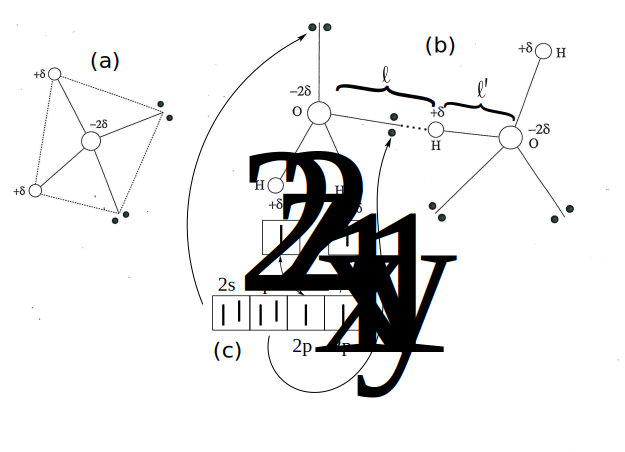
\includegraphics[width=10cm]{C8/figsC8/fig6G5.pdf}}
\caption{(\textbf{a}) To understand the behavior of water molecules one has to realize that in the covalent bonds, where the oxygen and the hydrogen atoms share a couple of electrons, the corresponding electronic cloud is somewhat more concentrated on the oxygen than on the hydrogen. The oxygen acquires a partial charge $-2\delta$ while each hydrogen gets a positive one $+\delta$. (\textbf{b}) Such charges give rise to an attractive electric force between  close lying molecules, in which the hydrogen atoms of a molecule points to the oxygen atom of the other molecule. One can view this attractive force as a type of chemical bond. It is known as hydrogen bond. It is of notice that also in this type of bond there is a component which implies the sharing of electrons. Furthermore, the hydrogen atom in an hydrogen bond does not just stick indiscriminantly to the the oxygen of another molecule. Being positively charged it goes where the electrons are. So the hydrogen bond is a bond between a hydrogen atom and a lone pair (two bold face dots). This means that a water molecule can form four hydrogen bonds: the molecule's two hydrogens form two bonds with neighboring oxygens, while the molecule's two lone pairs interact with neighboring hydrogens. (\textbf{c}) Schematic electronic structure of H$_2$O.}\label{fig6G5}
\end{figure}
\begin{figure}
\centerline{\includegraphics[width=10cm]{C8/figsC8/fig6G6.pdf}}
\caption{The water molecule is bent, with the two bonds between oxygen and hydrogen splayed at an angle of 104.5$^\circ$ \textbf{(a)}. To understand the structure of liquid water, we must also take into account the two ``lone pairs'' of electrons on the oxygen atom. The hydrogen atoms and the lone pairs sit more or less at the corners of a tetrahedron \textbf{(b)}. (after \cite{Ball:03}).}\label{fig6G6}
\end{figure}
\begin{figure}
\centerline{\includegraphics[width=6cm]{C8/figsC8/fig6G7.pdf}}
\caption{(Color online) Stick and ball representation (blue O, light grey H) of a network of hydrogen bonds in bulk water (after \cite{Chandler:02}). }\label{fig6G7}
\end{figure}
\begin{figure}
\centerline{\includegraphics[width=6cm]{C8/figsC8/fig6G8.pdf}}
\caption{Schematic representation of water molecules (arrowed lines also blue arrowed) impinging from the outside (liquid) and from the inter space (vapor) of two large parallel hydrophobic plates (after \cite{Lum:99}).}\label{fig6G8}
\end{figure}
Hybridization between the four orbitals $\ket{2s},\ket{2p_x},\ket{2p_y}$ and $\ket{2p_z}$ leads to a tetrahedral correlation in which the four orbitals $\ket{i}$ point towards the corners of a tetrahedron with the oxygen atom at the center (Fig. \ref{fig6G5} (a), \ref{fig6G6}). Because the electronic distribution has its charge center closer to the oxygen atom than to the two protons of the H--atoms, H$_2$O has a sizable dipole moment\footnote{The dipole moment of a polar molecule is defined as $u=ql$, where $l$ is the distance between the two charges $+q$ and $-q$. Thus, for two electronic charges $q=\pm e$ separated by $l=0.1$ nm, the dipole moment is $u=1.602\times 10^{-19}$ C$\times10^{-10}$ m=4.8 D, where the Debye=1D=3.336$\times10^{-30}$ Cm is the unit of dipole moment. Small polar molecules have moments of the order of 1D (see e.g. \cite{Israelachvili:85}). } ($\approx 0.68 ea_0\approx0.6$ D, $e$ being the electron charge, $a_0$ the Bohr radius and D the Debye unit). Water molecules can form four hydrogen bonds\footnote{Let us consider an H atom in a covalent bond with oxygen. When a second oxygen atom approaches the H atom, its nucleus, the proton, sees a potential with two minima, and tunnels through the corresponding barrier from one minimum to the other. In other words, the effective potential in which the proton moves becomes broader as compared to the single oxygen potential. Thus, the quantum mechanical confinement kinetic energy decreases by roughly a factor of two. This implies that the order of magnitude energy of an hydrogen bond between two oxygen atoms corresponds to the difference in the corresponding ZPF energies, i.e. $\approx200$ meV ($\approx 0.38$ eV-0.19 eV$\approx$ 0.2 eV$\approx$ 4.6 kcal/mol ($\approx8$ kT), where kT ($\approx0.6$ kcal/mol$\approx27$ meV) is the thermal energy at room temperature ($\approx310$ K)). For comparison a covalent  bond corresponds to $\approx96$ kcal/mol$\approx4$ eV, while the van der Waals interaction energy between two H at a distance of 2.4 \AA, that is of the order of the hydrogen bond length of 1.83 \AA,  is $\approx20$ meV (see \cite{Povh:02})} (hb), a special bond between molecules which is produced in situations when they share an hydrogen nucles between them. The molecule's two hydrogen atoms form two bonds with neighboring oxygens, while the molecule's two lone pairs interact with neighboring hydrogens\footnote{A possible pedestrian explanation of this is to impersonate a water molecule. Quoting from \cite{Ball:03}: ``Your hands are hydrogen atoms, your ankles are the lone pairs of electrons of oxygen. Stand legs apart\dots Twist 90$^\circ$ at the waist, stretch your arms and you're H$_2$O. The way that water molecules join up has just one rule: hands can grab ankles, but nothing else. That grasp is an hydrogen bond''.} (Figs. \ref{fig6G5} (b)). 


Water and oil do not mix. The term hydrophobic (water--fearing) is commonly used to describe substances that, like oil, do not mix (dissolves) with (in) water. Although it may look as if water repels oil, these two types of molecules actually attract each other, e.g. through the van der Waals interaction, but not nearly as strongly as water attracts itself. Mixing enough oil (hydrophobic, non polar (NP) molecules) with water leads to a reduction in favorable bonding. Strong mutual attraction between water molecules induce segregation of NP molecules from water and results in an effective NP--NP (hydrophobic) attraction, as observed e.g. in surface force measurements\footnote{See e.g. \cite{Chandler:02,Chandler:05} and \cite{Lum:99} and references therein.}. For example, the loss of hydrogen bonds near the two extended hydrophobic surfaces depicted in Fig. \ref{fig6G8} causes water to move away from those surfaces\footnote{Hydrophobic molecules do not hydrogen bond to water, creating excluded regions where the density of water molecules vanishes. When these units are small enough, water can reorganize near them without loosing hydrogen bonds, building an ice--like cage around the NP molecule. The entropic cost of this structural change leads to low solubility for small apolar molecules in water. Said it differently, such a force, known as the weak hydrophobic force (WHI) leads only to metastable states of groups of nonpolar molecules (\cite{Chandler:02}). On the other hand, close to a large hydrophobic object, the persistence of an hydrogen bond network --four bond per water molecule-- cannot persist, being geometrically impossible. In this case, water molecules near the hydrophobic cluster (surface) have typically three or fewer hydrogen bonds. This force, known as the strong hydrophobic force (SHI, \cite{Chandler:02}) can be viewed as a \textit{bona fide} hydrophobic interaction, stabilizing large aggregates of nonpolar molecules.}, producing thin vapour layers. Fluctuations in the interfaces form in this way can destabilize and expel the remaining liquid contained between these surfaces. The resulting pressure imbalance will cause the surfaces to attract. If the liquid is close to coexistence with the vapor phase, as is the case for water at ambient conditions, this phenomenon occurs for widely separated surfaces. The similarity with a (generalized) Casimir effect is apparent. Within this context, and in keeping with the fact that the hydrophobic force plays a central role in the folding and, as a consequence, in the biological activity of proteins, one can point that water at physiological conditions ($T=$300K, pH=7, etc.) can be viewed as the vacuum of the macromolecules responsible for metabolism, and thus one of the two origins of life on earth\footnote{To the question ``what is life?''(\cite{Schrodinger:44}) one is forced to answer that life is not one but two things (\cite{Dyson:99}). Which ones? Replication and metabolism. The molecules of DNA and RNA are responsible for the first function (\cite{Watson:53,Watson:80}), proteins (i.e. polymers made out of the 20 commonly occurring acids in nature), for the second (\cite{Sanger:52}). Because software (replication) is necessary a parasite of hardware (proteins), the becoming of a protein carries, to a large extent, the secret of life (\cite{Monod:70}).}.


While the many--body basis of hydrophobicity cannot be denied (Fig. \ref{fig6G7}) the parallel with the zero--body Casimir effect (Fig. \ref{fig6G3}) can hardly be avoided. Neither with the nuclear phenomena displayed in Fig. \ref{fig6G1} nor with those discussed in Sects. \ref{App3A2} and \ref{App3A3} in connection with superconductivity in metals.


Within this scenario, one can also observe a (generalized) Nambu-tumbling effect. Namely  the chain \textit{hydrogen bond$\to$ weak and strong hydrophobicity $\to$ polypeptide chain evolution$\to$ proteins (second order phase transition, spontaneous symmetry breaking in information space\footnote{\cite{Broglia:13b}.})$\to$ protein folding (first order phase transition in conformation space)$\to$ metabolism}. And, at the basis of the first link of the chain,  one finds the difference in the ZPF energy which an hydrogen nucleus feels when in presence of one (O) or two (O$_2$) oxygen nuclei, quantity closely connected with quantum fluctuation of confinement (\cite{Povh:02}).




\end{subappendices}
%\renewcommand{\bibname}{Bibliography Ch 7}
%\bibliographystyle{abbrvnat}
 %\bibliography{../nuclear_bib.bib}
%%\include{C8/Ch7NA}
\bibliographystyle{abbrvnat}
\renewcommand{\bibname}{Bibliography}
\bibliography{/home/gregory/book/nuclear_bib.bib}
\end{document} 